% Generated by Sphinx.
\def\sphinxdocclass{report}
\documentclass[letterpaper,10pt,english]{sphinxmanual}
\usepackage[utf8]{inputenc}
%\DeclareUnicodeCharacter{00A0}{\nobreakspace}
\usepackage{cmap}
\usepackage[T1]{fontenc}
\usepackage{babel}
\usepackage{times}
\usepackage[Bjarne]{fncychap}
\usepackage{longtable}
\usepackage{sphinx}
\usepackage{multirow}

\addto\captionsenglish{\renewcommand{\figurename}{Fig. }}
\addto\captionsenglish{\renewcommand{\tablename}{Table }}
\floatname{literal-block}{Listing }



\title{kOS Documentation}
\date{November 08, 2015}
\release{0.18.1}
\author{Dunbaratu, erendrake, Originally By Nivekk}
\newcommand{\sphinxlogo}{}
\renewcommand{\releasename}{Release}
\makeindex

\makeatletter
\def\PYG@reset{\let\PYG@it=\relax \let\PYG@bf=\relax%
    \let\PYG@ul=\relax \let\PYG@tc=\relax%
    \let\PYG@bc=\relax \let\PYG@ff=\relax}
\def\PYG@tok#1{\csname PYG@tok@#1\endcsname}
\def\PYG@toks#1+{\ifx\relax#1\empty\else%
    \PYG@tok{#1}\expandafter\PYG@toks\fi}
\def\PYG@do#1{\PYG@bc{\PYG@tc{\PYG@ul{%
    \PYG@it{\PYG@bf{\PYG@ff{#1}}}}}}}
\def\PYG#1#2{\PYG@reset\PYG@toks#1+\relax+\PYG@do{#2}}

\expandafter\def\csname PYG@tok@gd\endcsname{\def\PYG@tc##1{\textcolor[rgb]{0.63,0.00,0.00}{##1}}}
\expandafter\def\csname PYG@tok@gu\endcsname{\let\PYG@bf=\textbf\def\PYG@tc##1{\textcolor[rgb]{0.50,0.00,0.50}{##1}}}
\expandafter\def\csname PYG@tok@gt\endcsname{\def\PYG@tc##1{\textcolor[rgb]{0.00,0.27,0.87}{##1}}}
\expandafter\def\csname PYG@tok@gs\endcsname{\let\PYG@bf=\textbf}
\expandafter\def\csname PYG@tok@gr\endcsname{\def\PYG@tc##1{\textcolor[rgb]{1.00,0.00,0.00}{##1}}}
\expandafter\def\csname PYG@tok@cm\endcsname{\let\PYG@it=\textit\def\PYG@tc##1{\textcolor[rgb]{0.25,0.50,0.56}{##1}}}
\expandafter\def\csname PYG@tok@vg\endcsname{\def\PYG@tc##1{\textcolor[rgb]{0.73,0.38,0.84}{##1}}}
\expandafter\def\csname PYG@tok@m\endcsname{\def\PYG@tc##1{\textcolor[rgb]{0.13,0.50,0.31}{##1}}}
\expandafter\def\csname PYG@tok@mh\endcsname{\def\PYG@tc##1{\textcolor[rgb]{0.13,0.50,0.31}{##1}}}
\expandafter\def\csname PYG@tok@cs\endcsname{\def\PYG@tc##1{\textcolor[rgb]{0.25,0.50,0.56}{##1}}\def\PYG@bc##1{\setlength{\fboxsep}{0pt}\colorbox[rgb]{1.00,0.94,0.94}{\strut ##1}}}
\expandafter\def\csname PYG@tok@ge\endcsname{\let\PYG@it=\textit}
\expandafter\def\csname PYG@tok@vc\endcsname{\def\PYG@tc##1{\textcolor[rgb]{0.73,0.38,0.84}{##1}}}
\expandafter\def\csname PYG@tok@il\endcsname{\def\PYG@tc##1{\textcolor[rgb]{0.13,0.50,0.31}{##1}}}
\expandafter\def\csname PYG@tok@go\endcsname{\def\PYG@tc##1{\textcolor[rgb]{0.20,0.20,0.20}{##1}}}
\expandafter\def\csname PYG@tok@cp\endcsname{\def\PYG@tc##1{\textcolor[rgb]{0.00,0.44,0.13}{##1}}}
\expandafter\def\csname PYG@tok@gi\endcsname{\def\PYG@tc##1{\textcolor[rgb]{0.00,0.63,0.00}{##1}}}
\expandafter\def\csname PYG@tok@gh\endcsname{\let\PYG@bf=\textbf\def\PYG@tc##1{\textcolor[rgb]{0.00,0.00,0.50}{##1}}}
\expandafter\def\csname PYG@tok@ni\endcsname{\let\PYG@bf=\textbf\def\PYG@tc##1{\textcolor[rgb]{0.84,0.33,0.22}{##1}}}
\expandafter\def\csname PYG@tok@nl\endcsname{\let\PYG@bf=\textbf\def\PYG@tc##1{\textcolor[rgb]{0.00,0.13,0.44}{##1}}}
\expandafter\def\csname PYG@tok@nn\endcsname{\let\PYG@bf=\textbf\def\PYG@tc##1{\textcolor[rgb]{0.05,0.52,0.71}{##1}}}
\expandafter\def\csname PYG@tok@no\endcsname{\def\PYG@tc##1{\textcolor[rgb]{0.38,0.68,0.84}{##1}}}
\expandafter\def\csname PYG@tok@na\endcsname{\def\PYG@tc##1{\textcolor[rgb]{0.25,0.44,0.63}{##1}}}
\expandafter\def\csname PYG@tok@nb\endcsname{\def\PYG@tc##1{\textcolor[rgb]{0.00,0.44,0.13}{##1}}}
\expandafter\def\csname PYG@tok@nc\endcsname{\let\PYG@bf=\textbf\def\PYG@tc##1{\textcolor[rgb]{0.05,0.52,0.71}{##1}}}
\expandafter\def\csname PYG@tok@nd\endcsname{\let\PYG@bf=\textbf\def\PYG@tc##1{\textcolor[rgb]{0.33,0.33,0.33}{##1}}}
\expandafter\def\csname PYG@tok@ne\endcsname{\def\PYG@tc##1{\textcolor[rgb]{0.00,0.44,0.13}{##1}}}
\expandafter\def\csname PYG@tok@nf\endcsname{\def\PYG@tc##1{\textcolor[rgb]{0.02,0.16,0.49}{##1}}}
\expandafter\def\csname PYG@tok@si\endcsname{\let\PYG@it=\textit\def\PYG@tc##1{\textcolor[rgb]{0.44,0.63,0.82}{##1}}}
\expandafter\def\csname PYG@tok@s2\endcsname{\def\PYG@tc##1{\textcolor[rgb]{0.25,0.44,0.63}{##1}}}
\expandafter\def\csname PYG@tok@vi\endcsname{\def\PYG@tc##1{\textcolor[rgb]{0.73,0.38,0.84}{##1}}}
\expandafter\def\csname PYG@tok@nt\endcsname{\let\PYG@bf=\textbf\def\PYG@tc##1{\textcolor[rgb]{0.02,0.16,0.45}{##1}}}
\expandafter\def\csname PYG@tok@nv\endcsname{\def\PYG@tc##1{\textcolor[rgb]{0.73,0.38,0.84}{##1}}}
\expandafter\def\csname PYG@tok@s1\endcsname{\def\PYG@tc##1{\textcolor[rgb]{0.25,0.44,0.63}{##1}}}
\expandafter\def\csname PYG@tok@gp\endcsname{\let\PYG@bf=\textbf\def\PYG@tc##1{\textcolor[rgb]{0.78,0.36,0.04}{##1}}}
\expandafter\def\csname PYG@tok@sh\endcsname{\def\PYG@tc##1{\textcolor[rgb]{0.25,0.44,0.63}{##1}}}
\expandafter\def\csname PYG@tok@ow\endcsname{\let\PYG@bf=\textbf\def\PYG@tc##1{\textcolor[rgb]{0.00,0.44,0.13}{##1}}}
\expandafter\def\csname PYG@tok@sx\endcsname{\def\PYG@tc##1{\textcolor[rgb]{0.78,0.36,0.04}{##1}}}
\expandafter\def\csname PYG@tok@bp\endcsname{\def\PYG@tc##1{\textcolor[rgb]{0.00,0.44,0.13}{##1}}}
\expandafter\def\csname PYG@tok@c1\endcsname{\let\PYG@it=\textit\def\PYG@tc##1{\textcolor[rgb]{0.25,0.50,0.56}{##1}}}
\expandafter\def\csname PYG@tok@kc\endcsname{\let\PYG@bf=\textbf\def\PYG@tc##1{\textcolor[rgb]{0.00,0.44,0.13}{##1}}}
\expandafter\def\csname PYG@tok@c\endcsname{\let\PYG@it=\textit\def\PYG@tc##1{\textcolor[rgb]{0.25,0.50,0.56}{##1}}}
\expandafter\def\csname PYG@tok@mf\endcsname{\def\PYG@tc##1{\textcolor[rgb]{0.13,0.50,0.31}{##1}}}
\expandafter\def\csname PYG@tok@err\endcsname{\def\PYG@bc##1{\setlength{\fboxsep}{0pt}\fcolorbox[rgb]{1.00,0.00,0.00}{1,1,1}{\strut ##1}}}
\expandafter\def\csname PYG@tok@mb\endcsname{\def\PYG@tc##1{\textcolor[rgb]{0.13,0.50,0.31}{##1}}}
\expandafter\def\csname PYG@tok@ss\endcsname{\def\PYG@tc##1{\textcolor[rgb]{0.32,0.47,0.09}{##1}}}
\expandafter\def\csname PYG@tok@sr\endcsname{\def\PYG@tc##1{\textcolor[rgb]{0.14,0.33,0.53}{##1}}}
\expandafter\def\csname PYG@tok@mo\endcsname{\def\PYG@tc##1{\textcolor[rgb]{0.13,0.50,0.31}{##1}}}
\expandafter\def\csname PYG@tok@kd\endcsname{\let\PYG@bf=\textbf\def\PYG@tc##1{\textcolor[rgb]{0.00,0.44,0.13}{##1}}}
\expandafter\def\csname PYG@tok@mi\endcsname{\def\PYG@tc##1{\textcolor[rgb]{0.13,0.50,0.31}{##1}}}
\expandafter\def\csname PYG@tok@kn\endcsname{\let\PYG@bf=\textbf\def\PYG@tc##1{\textcolor[rgb]{0.00,0.44,0.13}{##1}}}
\expandafter\def\csname PYG@tok@o\endcsname{\def\PYG@tc##1{\textcolor[rgb]{0.40,0.40,0.40}{##1}}}
\expandafter\def\csname PYG@tok@kr\endcsname{\let\PYG@bf=\textbf\def\PYG@tc##1{\textcolor[rgb]{0.00,0.44,0.13}{##1}}}
\expandafter\def\csname PYG@tok@s\endcsname{\def\PYG@tc##1{\textcolor[rgb]{0.25,0.44,0.63}{##1}}}
\expandafter\def\csname PYG@tok@kp\endcsname{\def\PYG@tc##1{\textcolor[rgb]{0.00,0.44,0.13}{##1}}}
\expandafter\def\csname PYG@tok@w\endcsname{\def\PYG@tc##1{\textcolor[rgb]{0.73,0.73,0.73}{##1}}}
\expandafter\def\csname PYG@tok@kt\endcsname{\def\PYG@tc##1{\textcolor[rgb]{0.56,0.13,0.00}{##1}}}
\expandafter\def\csname PYG@tok@sc\endcsname{\def\PYG@tc##1{\textcolor[rgb]{0.25,0.44,0.63}{##1}}}
\expandafter\def\csname PYG@tok@sb\endcsname{\def\PYG@tc##1{\textcolor[rgb]{0.25,0.44,0.63}{##1}}}
\expandafter\def\csname PYG@tok@k\endcsname{\let\PYG@bf=\textbf\def\PYG@tc##1{\textcolor[rgb]{0.00,0.44,0.13}{##1}}}
\expandafter\def\csname PYG@tok@se\endcsname{\let\PYG@bf=\textbf\def\PYG@tc##1{\textcolor[rgb]{0.25,0.44,0.63}{##1}}}
\expandafter\def\csname PYG@tok@sd\endcsname{\let\PYG@it=\textit\def\PYG@tc##1{\textcolor[rgb]{0.25,0.44,0.63}{##1}}}

\def\PYGZbs{\char`\\}
\def\PYGZus{\char`\_}
\def\PYGZob{\char`\{}
\def\PYGZcb{\char`\}}
\def\PYGZca{\char`\^}
\def\PYGZam{\char`\&}
\def\PYGZlt{\char`\<}
\def\PYGZgt{\char`\>}
\def\PYGZsh{\char`\#}
\def\PYGZpc{\char`\%}
\def\PYGZdl{\char`\$}
\def\PYGZhy{\char`\-}
\def\PYGZsq{\char`\'}
\def\PYGZdq{\char`\"}
\def\PYGZti{\char`\~}
% for compatibility with earlier versions
\def\PYGZat{@}
\def\PYGZlb{[}
\def\PYGZrb{]}
\makeatother

\renewcommand\PYGZsq{\textquotesingle}

\begin{document}

\maketitle
\tableofcontents
\phantomsection\label{index::doc}


\textbf{kOS} is a scriptable autopilot modification for \textbf{Kerbal Space Program}. It allows you write small programs that automate specific tasks.


\chapter{Downloads and Video Links}
\label{downloads_links:downloads-and-video-links}\label{downloads_links:index}\label{downloads_links::doc}\label{downloads_links:welcome-to-the-kos-documentation-website}\begin{quote}

Useful link resources for kOS:
\end{quote}


\section{Obtaining kOS itself}
\label{downloads_links:obtain}\label{downloads_links:obtaining-kos-itself}\begin{quote}

The kOS mod can be obtained a number of ways:
\begin{itemize}
\item {} 
\href{https://github.com/KSP-CKAN/CKAN/releases}{Use CKAN}.  The Comprehensive Kerbal
Archive Network.  If you install the CKAN program, it can manage your mods for you
and check for updates whenever you run it.  kOS sends update information to CKAN
so kOS updates should appear in your CKAN manager tool as soon as they're released.

\item {} 
\href{https://github.com/KSP-KOS/KOS/releases}{Download from github directly}
Github is where development of the mod occurs, and new releases will apear there
first, without delays, and its where old obsolete releases can be found, if you
need one for use with an older version of KSP.

\item {} 
\href{https://kerbalstuff.com/mod/86/kOS:\%20Scriptable\%20Autopilot\%20System}{Use KerbalStuff}
Kerbalstuff is a community supported Kerbal Space Program mod hosting site that behaves
much like Curse, but without Curse's embedded advertisements all over the webpage.

\item {} 
\href{http://www.curse.com/ksp-mods/kerbal/220265-kos-scriptable-autopilot-system}{Download from Curse}
Love it or Loathe it, Curse is the official place SQUAD points people to for KSP addons, so we
make it available there too.

\end{itemize}
\end{quote}


\section{Change Log}
\label{downloads_links:change-log}\label{downloads_links:changelog}\begin{itemize}
\item {} 
\href{https://github.com/KSP-KOS/KOS/blob/develop/CHANGELOG.md}{Change Log} on Github.

\end{itemize}


\section{Show and Tell, and Tutorials}
\label{downloads_links:show-and-tell-and-tutorials}\label{downloads_links:showandtell}\begin{quote}

There are a number of people who have created helpful tutorials for kOS, and
others who've created show and tell videos showing the nifty things they've done with kOS.
If you'd like to have your video added to this section please contact the authors of
over on github at \href{https://github.com/KSP-KOS/KOS}{https://github.com/KSP-KOS/KOS}.

Note that there is category overlap as often a showoff video is also a sort of tutorial too.
\end{quote}

\textbf{Tutorials}
\begin{itemize}
\item {} 
\href{https://www.youtube.com/playlist?list=PLEpK8nolWr1rghS5cOEOL-JQ33h4CgPAP}{Seth Persigehl's Tutorial playlist}

\end{itemize}

\textbf{Show and Tell}
\begin{itemize}
\item {} 
\href{https://www.youtube.com/playlist?list=PLdXwd2JlyAvqamZN\_jfcxUc29Q6Kzxqmb}{Steven Mading's user scripts playlist}
Some of these are very old and out of date, going back as far as kOS version 0.65.  The actual code
used may have to be tweaked a bit to work with recent kOS releases.

\item {} 
\href{http://www.reddit.com/r/Kos/comments/2w3sq5/first\_working\_docking\_script\_info\_in\_comments/}{Parasite's first docking script, reddit post}

\end{itemize}

\textbf{Past Teasers}
\begin{itemize}
\item {} 
\href{https://www.youtube.com/playlist?list=PLdXwd2JlyAvo\_pH1tS3P7elVTYjvmIh-m}{Steven Mading's Developer teasers playlist}
(Note these are teasers that were created just before new features were first released, to
show off what was (at the time) new content that hadn't been public yet.  They also can
constitute a tutorial of sorts to show how some of the features work.)

\end{itemize}


\chapter{Tutorials}
\label{tutorials:tutorials}\label{tutorials::doc}\label{tutorials:id1}
If you prefer the tutorial style of explanation, please see the following examples that walk you through examples:


\section{Quick Start Tutorial}
\label{tutorials/quickstart::doc}\label{tutorials/quickstart:quickstart}\label{tutorials/quickstart:quick-start-tutorial}
This is a quick start guide for the \textbf{Kerbal Operating System} (\textbf{kOS}). It is intended for those who are just starting with using \textbf{kOS}. It does presume you have played \textbf{Kerbal Space Program} before and know the basics of how to fly a rocket under manual control. It does \emph{NOT} assume you know a lot about computer programming, and it will walk you through some basic first steps.
\setbox0\vbox{
\begin{minipage}{0.95\linewidth}
\textbf{Contents}

\medskip

\begin{itemize}
\item {} 
\phantomsection\label{tutorials/quickstart:id1}{\hyperref[tutorials/quickstart:first-example-hello-world]{\emph{First example: Hello World}}}
\begin{itemize}
\item {} 
\phantomsection\label{tutorials/quickstart:id2}{\hyperref[tutorials/quickstart:step-1-start-a-new-sandbox-mode-game]{\emph{Step 1: Start a new sandbox-mode game}}}

\item {} 
\phantomsection\label{tutorials/quickstart:id3}{\hyperref[tutorials/quickstart:step-2-make-a-vessel-in-the-vehicle-assembly-bay]{\emph{Step 2: Make a vessel in the Vehicle Assembly Bay}}}

\item {} 
\phantomsection\label{tutorials/quickstart:id4}{\hyperref[tutorials/quickstart:step-3-put-the-vessel-on-the-launchpad]{\emph{Step 3: Put the vessel on the launchpad}}}

\item {} 
\phantomsection\label{tutorials/quickstart:id5}{\hyperref[tutorials/quickstart:step-4-invoke-the-terminal]{\emph{Step 4: Invoke the terminal}}}

\item {} 
\phantomsection\label{tutorials/quickstart:id6}{\hyperref[tutorials/quickstart:step-5-see-what-an-interactive-command-is-like]{\emph{Step 5: See what an interactive command is like}}}

\item {} 
\phantomsection\label{tutorials/quickstart:id7}{\hyperref[tutorials/quickstart:step-6-okay-that-s-great-but-how-can-you-make-that-happen-in-a-program-script-instead]{\emph{Step 6: Okay that's great, but how can you make that happen in a program script instead?}}}

\item {} 
\phantomsection\label{tutorials/quickstart:id8}{\hyperref[tutorials/quickstart:step-7-okay-but-where-is-this-program]{\emph{Step 7: Okay, but where is this program?}}}

\item {} 
\phantomsection\label{tutorials/quickstart:id9}{\hyperref[tutorials/quickstart:step-8-i-don-t-like-the-idea-that-the-program-is-stored-only-on-this-vessel-can-t-i-save-it-somewhere-better-more-permanent]{\emph{Step 8: I don't like the idea that the program is stored only on this vessel. Can't I save it somewhere better? More permanent?}}}

\end{itemize}

\item {} 
\phantomsection\label{tutorials/quickstart:id10}{\hyperref[tutorials/quickstart:second-example-doing-something-real]{\emph{Second Example: Doing something real}}}
\begin{itemize}
\item {} 
\phantomsection\label{tutorials/quickstart:id11}{\hyperref[tutorials/quickstart:step-1-make-a-vessel]{\emph{Step 1: Make a vessel}}}

\item {} 
\phantomsection\label{tutorials/quickstart:id12}{\hyperref[tutorials/quickstart:step-2-make-the-start-of-the-script]{\emph{Step 2: Make the start of the script}}}

\item {} 
\phantomsection\label{tutorials/quickstart:id13}{\hyperref[tutorials/quickstart:step-3-make-the-script-actually-do-something]{\emph{Step 3: Make the script actually do something}}}

\item {} 
\phantomsection\label{tutorials/quickstart:id14}{\hyperref[tutorials/quickstart:step-4-make-the-script-actually-control-steering]{\emph{Step 4: Make the script actually control steering}}}

\item {} 
\phantomsection\label{tutorials/quickstart:id15}{\hyperref[tutorials/quickstart:step-5-add-staging-logic]{\emph{Step 5: Add staging logic}}}

\item {} 
\phantomsection\label{tutorials/quickstart:id16}{\hyperref[tutorials/quickstart:step-6-now-to-make-it-turn]{\emph{Step 6: Now to make it turn}}}

\item {} 
\phantomsection\label{tutorials/quickstart:id17}{\hyperref[tutorials/quickstart:step-7-putting-it-all-together]{\emph{Step 7: Putting it all together}}}

\end{itemize}

\end{itemize}
\end{minipage}}
\begin{center}\setlength{\fboxsep}{5pt}\shadowbox{\box0}\end{center}


\subsection{First example: Hello World}
\label{tutorials/quickstart:first-example-hello-world}
In the grand tradition of programming tutorials, the first example will be how to make a script that does nothing more than print the words ``Hello World'' on the screen. The purpose of this example is to show where you should put the files, how to move them about, and how to get one to run on the vessel.


\subsubsection{Step 1: Start a new sandbox-mode game}
\label{tutorials/quickstart:step-1-start-a-new-sandbox-mode-game}
(You can use \textbf{kOS} in a career mode game, but it requires a part that you have to research which isn't available at the start of the tech tree, so this example will just use sandbox mode to keep it simple.)


\subsubsection{Step 2: Make a vessel in the Vehicle Assembly Bay}
\label{tutorials/quickstart:step-2-make-a-vessel-in-the-vehicle-assembly-bay}
Make the vessel contain any unmanned command core, a few hundred units of battery power, a means of recharging the battery such as a solar panel array, and the ``Comptronix CX-4181 Scriptable Control System''. (From this point onward the CX-4181 Scriptable Control System part will be referred to by the acronym ``SCS''.) The SCS part is located in the parts bin under the ``Control'' tab (the same place where RCS thrusters and Torque Wheels are found.)
\begin{figure}[htbp]
\centering

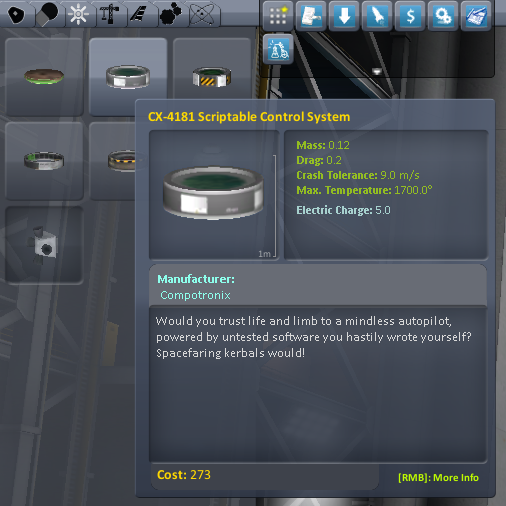
\includegraphics{SCS_parts_bin.png}
\end{figure}


\subsubsection{Step 3: Put the vessel on the launchpad}
\label{tutorials/quickstart:step-3-put-the-vessel-on-the-launchpad}
Put the vessel on the launchpad. For this first example it doesn't matter if the vessel can actually liftoff or even has engines at all.


\subsubsection{Step 4: Invoke the terminal}
\label{tutorials/quickstart:step-4-invoke-the-terminal}
Right click for the SCS part on the vessel and then click the button that says ``Open Terminal''.

Note that if the terminal is semi-transparent, this means it's not currently selected. If you click on the terminal, then your keyboard input is directed to the terminal INSTEAD of to piloting. In other words if you type \code{W} \code{A} \code{S} \code{D}, you'll actually get the word ``wasd'' to appear on the terminal, rather than the \code{W} \code{A} \code{S} \code{D} keys steering the ship. To switch back to manual control of the game instead of typing into the terminal, click outside the terminal window anywhere on the background of the screen.


\subsubsection{Step 5: See what an interactive command is like}
\label{tutorials/quickstart:step-5-see-what-an-interactive-command-is-like}
You should now see an old-school looking text terminal like the one shown below. Type the line:

\begin{Verbatim}[commandchars=\\\{\}]
\PYG{n}{CLEARSCREEN}\PYG{p}{.} \PYG{n}{PRINT} \PYG{l+s}{\PYGZdq{}}\PYG{l+s}{==HELLO WORLD==}\PYG{l+s}{\PYGZdq{}}\PYG{p}{.}
\end{Verbatim}

into the terminal (make sure to actually type the periods (''.'') as shown) and hit \code{ENTER}. Note that you can type it in uppercase or lowercase. \textbf{kOS} doesn't care.
\begin{figure}[htbp]
\centering

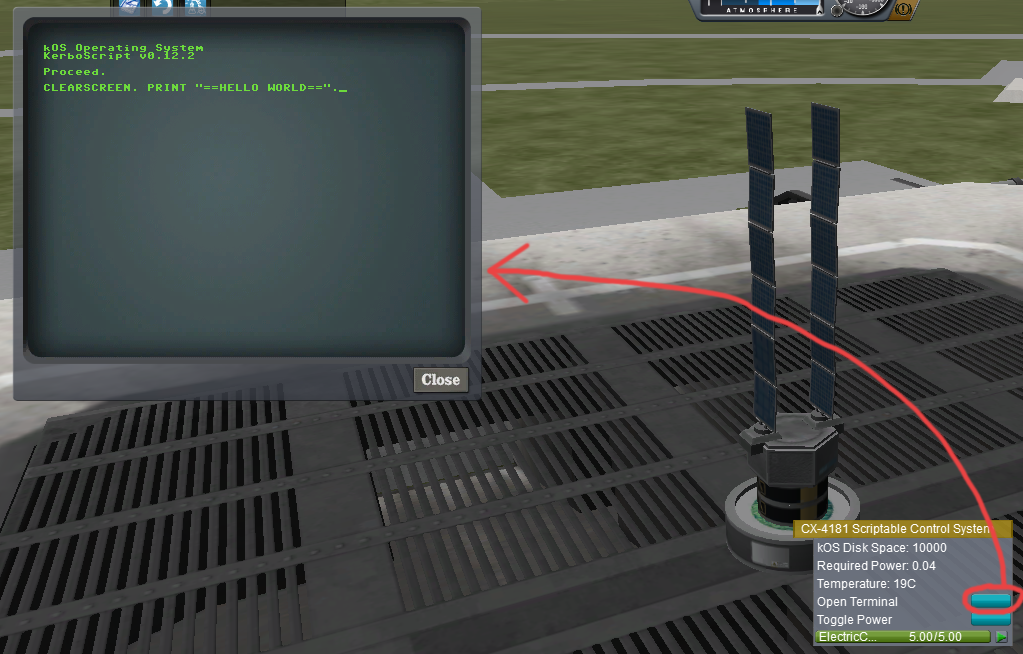
\includegraphics[width=0.800\linewidth]{terminal_open_1.png}
\end{figure}

The terminal will respond by showing you this:
\begin{figure}[htbp]
\centering

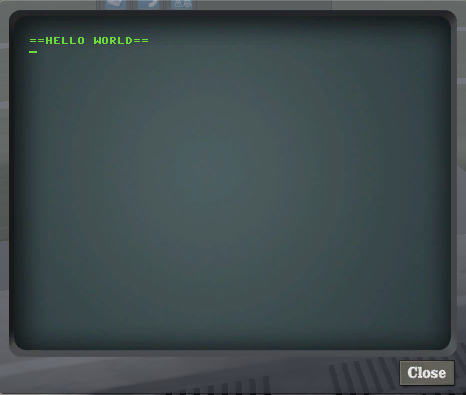
\includegraphics{terminal_open_2.png}
\end{figure}


\subsubsection{Step 6: Okay that's great, but how can you make that happen in a program script instead?}
\label{tutorials/quickstart:step-6-okay-that-s-great-but-how-can-you-make-that-happen-in-a-program-script-instead}
Like so: Enter this command:

\begin{Verbatim}[commandchars=\\\{\}]
\PYG{n}{EDIT} \PYG{n}{HELLO}\PYG{p}{.}
\end{Verbatim}

(Don't forget the period (''.''). All commands in \textbf{kOS} are ended with a period. Again, you can type it in uppercase or lowercase. \textbf{kOS} doesn't care.)

You should see an editor window appear, looking something like this (without the text inside because you're starting a blank new file):
\begin{figure}[htbp]
\centering

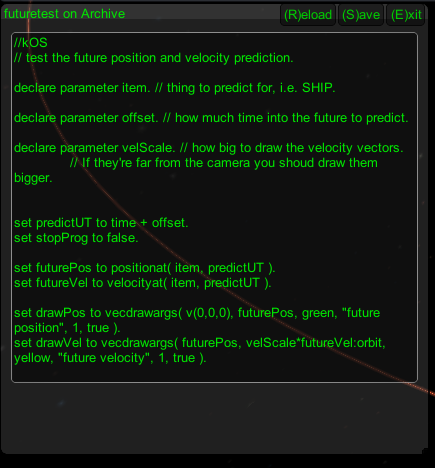
\includegraphics{editor.png}
\end{figure}

Type this text into the window:

\begin{Verbatim}[commandchars=\\\{\}]
\PYG{n}{PRINT} \PYG{l+s}{\PYGZdq{}}\PYG{l+s}{=========================================}\PYG{l+s}{\PYGZdq{}}\PYG{p}{.}
\PYG{n}{PRINT} \PYG{l+s}{\PYGZdq{}}\PYG{l+s}{      HELLO WORLD}\PYG{l+s}{\PYGZdq{}}\PYG{p}{.}
\PYG{n}{PRINT} \PYG{l+s}{\PYGZdq{}}\PYG{l+s}{THIS IS THE FIRST SCRIPT I WROTE IN kOS.}\PYG{l+s}{\PYGZdq{}}\PYG{p}{.}
\PYG{n}{PRINT} \PYG{l+s}{\PYGZdq{}}\PYG{l+s}{=========================================}\PYG{l+s}{\PYGZdq{}}\PYG{p}{.}
\end{Verbatim}

Click ``Save'' then ``Exit'' in the editor pop-up window.
\begin{itemize}
\item {} 
\emph{Side Note: The editor font} - Experienced programmers may have noticed that the editor's font is proportional width rather than monospaced and that this is not ideal for programming work. You are right, but there is little that can be done about it for a variety of technical reasons that are too complex to go into right now.

\end{itemize}

Then on the main text terminal Enter:

\begin{Verbatim}[commandchars=\\\{\}]
\PYG{n}{RUN} \PYG{n}{HELLO}\PYG{p}{.}
\end{Verbatim}

And you will see the program run, showing the text on the screen like so.
\begin{figure}[htbp]
\centering

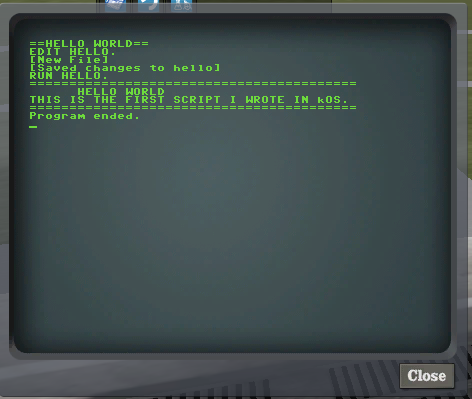
\includegraphics{hello_world1.png}
\end{figure}


\subsubsection{Step 7: Okay, but where is this program?}
\label{tutorials/quickstart:step-7-okay-but-where-is-this-program}
To see where the ``HELLO'' program has been saved, Issue the command \code{LIST FILES} like this:

\begin{Verbatim}[commandchars=\\\{\}]
\PYG{n}{LIST} \PYG{n}{FILES}\PYG{p}{.}
\end{Verbatim}

(Note, that the default for the \code{LIST} command is to list \code{FILES}, so you can leave the word ``FILES'' off if you like.)

It should look like this, showing you the HELLO program you just wrote:
\begin{figure}[htbp]
\centering

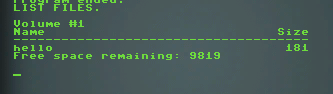
\includegraphics{hello_list.png}
\end{figure}

This is a list of all the files on the currently selected VOLUME. By default, when you launch a new vessel, the currently selected VOLUME is called ``1'' and it's the volume that's stored on THAT SCS part that you are running all these commands in.

This is the local volume of that SCS part. Local volumes such at this tend to have very small limited storage, as you can see when you look at the space remaining in the list printout.

If you're wondering where the file is stored \emph{physically} on your computer, it's represented by a section inside the persistence file for your saved game, as a piece of data associated with the SCS part. This is important because it means you can't access the program from another vessel, and if this vessel ever crashes and the SCS part explodes, then you've lost the program.


\subsubsection{Step 8: I don't like the idea that the program is stored only on this vessel. Can't I save it somewhere better? More permanent?}
\label{tutorials/quickstart:step-8-i-don-t-like-the-idea-that-the-program-is-stored-only-on-this-vessel-can-t-i-save-it-somewhere-better-more-permanent}
Yes. Yes you can.

There is another VOLUME that always exists called the \emph{Archive}, which is also referred to as volume 0. (either name can be used in commands). The archive is conceptually stored somewhere back at Kerbin home base in the Space Center rather than on your vessel. It has infinite storage space, and does not disappear when your vessel is gone. ALSO, it actually exists across saved games - if you launch one saved game, put a new file in the Archive, and then later launch a different saved game, that file will be there in that game too.

To use the Archive, first we'll have to introduce you to a new command, called \code{SWITCH TO}. The \code{SWITCH TO} command changes which VOLUME is the one that you are doing your work with.

To work with the archive, and create a second ``hello world'' file there, you issue these commands and see what they do:

\begin{Verbatim}[commandchars=\\\{\}]
\PYG{n}{SWITCH} \PYG{n}{TO} \PYG{l+m+mf}{0.}
\PYG{n}{EDIT} \PYG{n}{HELLO2}\PYG{p}{.} \PYG{c+c1}{// Make a new file here that just says: PRINT \PYGZdq{}hi again\PYGZdq{}.}
\PYG{n}{LIST} \PYG{n}{FILES}\PYG{p}{.}
\PYG{n}{RUN} \PYG{n}{HELLO2}\PYG{p}{.}
\PYG{n}{SWITCH} \PYG{n}{TO} \PYG{l+m+mf}{1.}
\PYG{n}{LIST} \PYG{n}{FILES}\PYG{p}{.}
\PYG{n}{RUN} \PYG{n}{HELLO}\PYG{p}{.}
\end{Verbatim}

\emph{But where is it stored behind the scenes?} The archive is currently slightly violating the design of \textbf{KSP} mods that puts everything in the GameData folder. The kSP Archive is actually stored in the \code{Ships/Script} folder of your MAIN \textbf{KSP} home, not inside GameData.

If a file is stored inside the archive, it can actually be edited \emph{by an external text editor of your choice} instead of using \textbf{kOS}`s in-game editor. This is usually a much better practice once you start doing more complex things with \textbf{kOS}. You can also make new files in the archive folder. Just make sure that all the files end with a \code{.ks} file name suffix or \textbf{kOS} won't use them.

Further reading about files and volumes:
\begin{itemize}
\item {} 
{\hyperref[general/volumes:volumes]{\emph{\DUspan{}{Volumes}}}}

\item {} 
{\hyperref[commands/files:files]{\emph{\DUspan{}{File Control}}}}

\item {} 
{\hyperref[structures/misc/fileinfo:fileinfo]{\emph{\DUspan{}{File Information}}}}

\end{itemize}


\subsection{Second Example: Doing something real}
\label{tutorials/quickstart:second-example-doing-something-real}
Okay that's all basic setup stuff but you're probably clamoring for a real example that actually does something nifty.

This example will show the crudest, most basic use of \textbf{kOS} just to get started. In this example we'll make a program that will launch a vessel using progressively more and more complex checks. \textbf{kOS} can be used at any stage of a vessel's flight - launching, circularizing, docking, landing,... and in fact launching is one of the simpler piloting tasks that you can do without much need of automation. Where \textbf{kOS} really shines is for writing scripts to do touchy sensitive tasks like landing or docking or hovering. These are the areas that can benefit from the faster reaction speed that a computer script can handle.

But in order to give you an example that you can start with from scratch, that's easy to reload and retry from an initial point, we'll use an example of launching.


\subsubsection{Step 1: Make a vessel}
\label{tutorials/quickstart:step-1-make-a-vessel}
This tutorial is designed to work with a very specific rocket design.
You need to make the vessel you see here:
\begin{figure}[htbp]
\centering

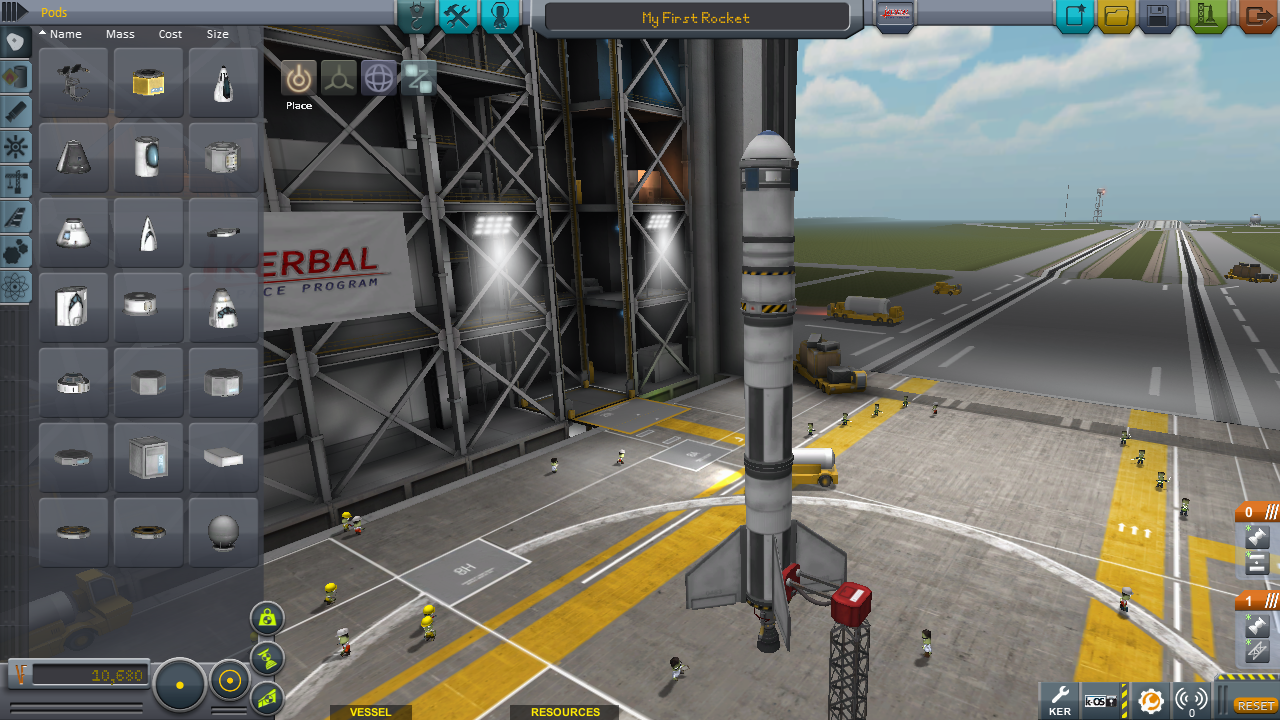
\includegraphics[width=0.800\linewidth]{example_2_0.png}
\end{figure}

If you prefer, you can instead download the
.craft file here


\subsubsection{Step 2: Make the start of the script}
\label{tutorials/quickstart:step-2-make-the-start-of-the-script}
Okay, so type the lines below in an external \emph{text editor of your choice} (i.e. Notepad on Windows, or TextEdit on Mac, or whatever you fancy):

\begin{Verbatim}[commandchars=\\\{\}]
\PYG{c+c1}{//hellolaunch}

\PYG{c+c1}{//First, we\PYGZsq{}ll clear the terminal screen to make it look nice}
\PYG{n}{CLEARSCREEN}\PYG{p}{.}

\PYG{c+c1}{//This is our countdown loop, which cycles from 10 to 0}
\PYG{n}{PRINT} \PYG{l+s}{\PYGZdq{}}\PYG{l+s}{Counting down:}\PYG{l+s}{\PYGZdq{}}\PYG{p}{.}
\PYG{n}{FROM} \PYG{p}{\PYGZob{}}\PYG{n}{local} \PYG{n}{countdown} \PYG{n}{is} \PYG{l+m+mf}{10.}\PYG{p}{\PYGZcb{}} \PYG{n}{UNTIL} \PYG{n}{countdown} \PYG{o}{=} \PYG{l+m+mi}{0} \PYG{n}{STEP} \PYG{p}{\PYGZob{}}\PYG{n}{SET} \PYG{n}{countdown} \PYG{n}{to} \PYG{n}{countdown} \PYG{o}{\PYGZhy{}} \PYG{l+m+mf}{1.}\PYG{p}{\PYGZcb{}} \PYG{n}{DO} \PYG{p}{\PYGZob{}}
    \PYG{n}{PRINT} \PYG{l+s}{\PYGZdq{}}\PYG{l+s}{...}\PYG{l+s}{\PYGZdq{}} \PYG{o}{+} \PYG{n}{countdown}\PYG{p}{.}
    \PYG{n}{WAIT} \PYG{l+m+mf}{1.} \PYG{c+c1}{// pauses the script here for 1 second.}
\PYG{p}{\PYGZcb{}}
\end{Verbatim}

See those things with the two slashes (``//'')? Those are comments in the kerboscript language and they're just ways to write things in the program that don't do anything - they're there for humans like you to read so you understand what's going on. In these examples you never actually have to type in the things you see after the slashes. They're there for your benefit when reading this document but you can leave them out if you wish.

Save the file in your \code{Ships/Script} folder of your \textbf{KSP} installation under the filename ``hellolaunch.ks''. DO NOT save it anywhere under \code{GameData/kOS/}. Do NOT. According to the \textbf{KSP} standard, normally \textbf{KSP} mods should put their files in \code{GameData/{[}mod name{]}}, but \textbf{kOS} puts the archive outside the \code{GameData} folder because it represents content owned by you, the player, not content owned by the \textbf{kOS} mod.

By saving the file in \code{Ships/Script}, you have actually put it in your archive volume of \textbf{kOS}. \textbf{kOS} will see it there immediately without delay. You do not need to restart the game. If you do:

\begin{Verbatim}[commandchars=\\\{\}]
\PYG{n}{SWITCH} \PYG{n}{TO} \PYG{l+m+mf}{0.}
\PYG{n}{LIST} \PYG{n}{FILES}\PYG{p}{.}
\end{Verbatim}

after saving the file from your external text editor program, you will see a listing of your file ``hellolaunch'' right away. Okay, now copy it to your local drive and give it a try running it from there:

\begin{Verbatim}[commandchars=\\\{\}]
\PYG{n}{SWITCH} \PYG{n}{TO} \PYG{l+m+mf}{1.}
\PYG{n}{COPY} \PYG{n}{HELLOLAUNCH} \PYG{n}{FROM} \PYG{l+m+mf}{0.}
\PYG{n}{RUN} \PYG{n}{HELLOLAUNCH}\PYG{p}{.}
\end{Verbatim}
\begin{figure}[htbp]
\centering

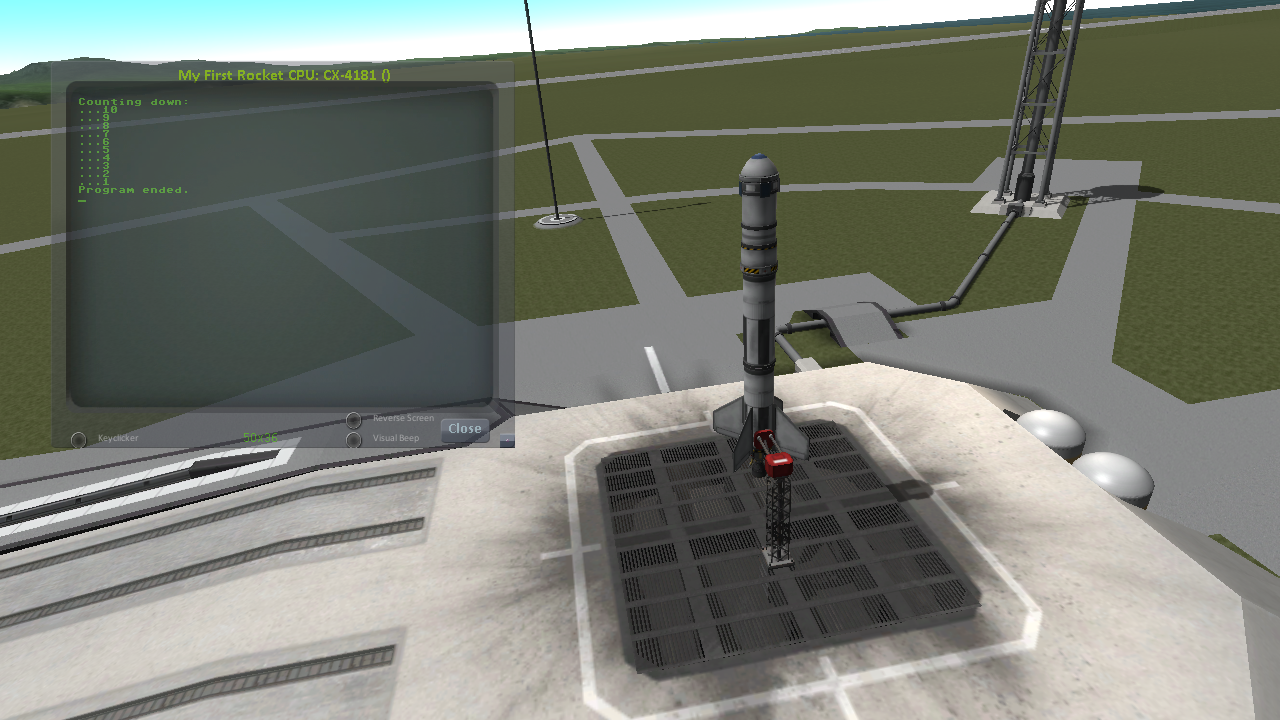
\includegraphics[width=0.800\linewidth]{example_2_1.png}
\end{figure}

Okay so the program doesn't actually DO anything yet other than just countdown from 10 to 0. A bit of a disappointment, but we haven't written the rest of the program yet.

You'll note that what you've done is switch to the local volume (1) and then copy the program from the archive (0) to the local volume (1) and then run it from the local volume. Technically you didn't need to do this. You could have just run it directly from the archive. For those looking at the \textbf{KSP} game as a bit of a role-play experience, it makes sense to never run programs directly from the archive, and instead live with the limitation that software should be copied to the craft for it to be able to run it.


\subsubsection{Step 3: Make the script actually do something}
\label{tutorials/quickstart:step-3-make-the-script-actually-do-something}
Okay now go back into your \emph{text editor of choice} and append a few more lines to the hellolaunch.ks file so it now looks like this:

\begin{Verbatim}[commandchars=\\\{\}]
\PYG{c+c1}{//hellolaunch}

\PYG{c+c1}{//First, we\PYGZsq{}ll clear the terminal screen to make it look nice}
\PYG{n}{CLEARSCREEN}\PYG{p}{.}

\PYG{c+c1}{//Next, we\PYGZsq{}ll lock our throttle to 100\PYGZpc{}.}
\PYG{n}{LOCK} \PYG{n}{THROTTLE} \PYG{n}{TO} \PYG{l+m+mf}{1.0}\PYG{p}{.}   \PYG{c+c1}{// 1.0 is the max, 0.0 is idle.}

\PYG{c+c1}{//This is our countdown loop, which cycles from 10 to 0}
\PYG{n}{PRINT} \PYG{l+s}{\PYGZdq{}}\PYG{l+s}{Counting down:}\PYG{l+s}{\PYGZdq{}}\PYG{p}{.}
\PYG{n}{FROM} \PYG{p}{\PYGZob{}}\PYG{n}{local} \PYG{n}{countdown} \PYG{n}{is} \PYG{l+m+mf}{10.}\PYG{p}{\PYGZcb{}} \PYG{n}{UNTIL} \PYG{n}{countdown} \PYG{o}{=} \PYG{l+m+mi}{0} \PYG{n}{STEP} \PYG{p}{\PYGZob{}}\PYG{n}{SET} \PYG{n}{countdown} \PYG{n}{to} \PYG{n}{countdown} \PYG{o}{\PYGZhy{}} \PYG{l+m+mf}{1.}\PYG{p}{\PYGZcb{}} \PYG{n}{DO} \PYG{p}{\PYGZob{}}
    \PYG{n}{PRINT} \PYG{l+s}{\PYGZdq{}}\PYG{l+s}{...}\PYG{l+s}{\PYGZdq{}} \PYG{o}{+} \PYG{n}{countdown}\PYG{p}{.}
    \PYG{n}{WAIT} \PYG{l+m+mf}{1.} \PYG{c+c1}{// pauses the script here for 1 second.}
\PYG{p}{\PYGZcb{}}

\PYG{n}{UNTIL} \PYG{n+nl}{SHIP}\PYG{p}{:}\PYG{n}{MAXTHRUST} \PYG{o}{\PYGZgt{}} \PYG{l+m+mi}{0} \PYG{p}{\PYGZob{}}
    \PYG{n}{WAIT} \PYG{l+m+mf}{0.5}\PYG{p}{.} \PYG{c+c1}{// pause half a second between stage attempts.}
    \PYG{n}{PRINT} \PYG{l+s}{\PYGZdq{}}\PYG{l+s}{Stage activated.}\PYG{l+s}{\PYGZdq{}}\PYG{p}{.}
    \PYG{n}{STAGE}\PYG{p}{.} \PYG{c+c1}{// same as hitting the spacebar.}
\PYG{p}{\PYGZcb{}}

\PYG{n}{WAIT} \PYG{n}{UNTIL} \PYG{n+nl}{SHIP}\PYG{p}{:}\PYG{n}{ALTITUDE} \PYG{o}{\PYGZgt{}} \PYG{l+m+mf}{70000.}

\PYG{c+c1}{// NOTE that it is vital to not just let the script end right away}
\PYG{c+c1}{// here.  Once a kOS script just ends, it releases all the controls}
\PYG{c+c1}{// back to manual piloting so that you can fly the ship by hand again.}
\PYG{c+c1}{// If the program just ended here, then that would cause the throttle}
\PYG{c+c1}{// to turn back off again right away and nothing would happen.}
\end{Verbatim}

Save this file to hellolaunch.ks again, and re-copy it to your vessel that should still be sitting on the launchpad, then run it, like so:

\begin{Verbatim}[commandchars=\\\{\}]
\PYG{n}{COPY} \PYG{n}{HELLOLAUNCH} \PYG{n}{FROM} \PYG{l+m+mf}{0.}
\PYG{n}{RUN} \PYG{n}{HELLOLAUNCH}\PYG{p}{.}
\end{Verbatim}
\begin{figure}[htbp]
\centering

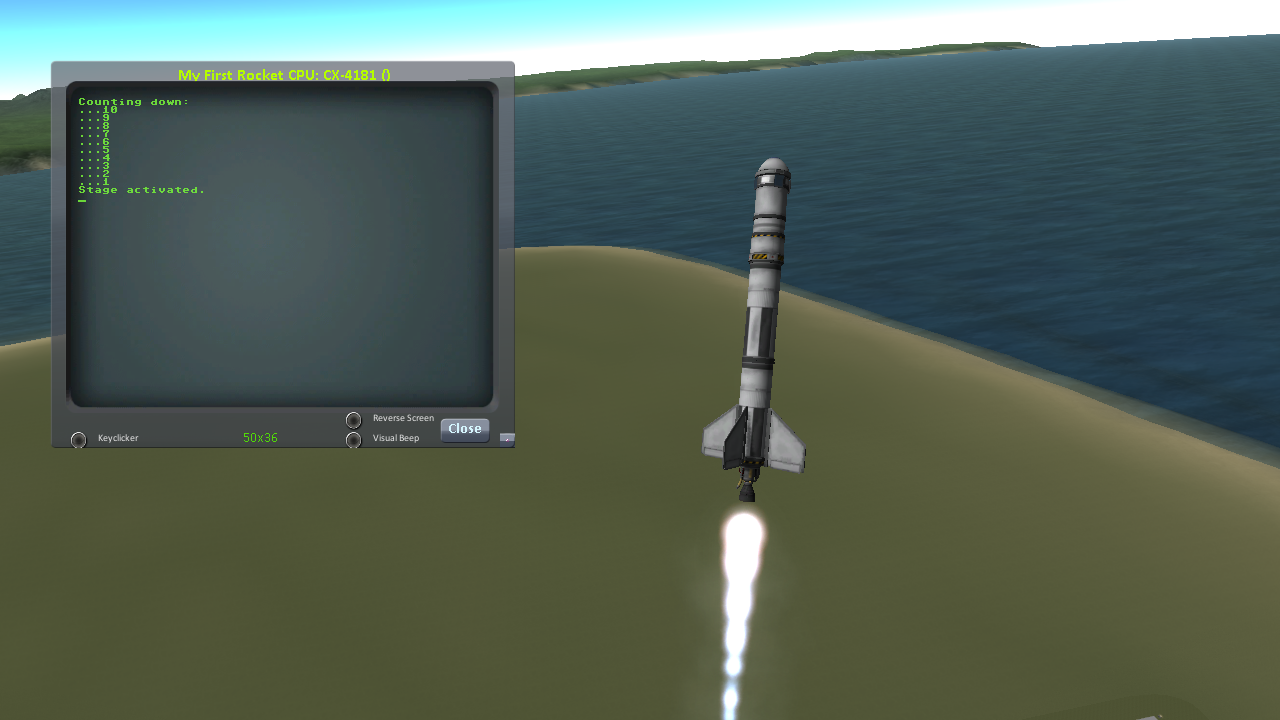
\includegraphics[width=0.800\linewidth]{example_2_2.png}
\end{figure}

Hey! It does something now! It fires the first stage engine and launches!

But.. but wait... It doesn't control the steering and it just lets it go where ever it will.

Most likely you had a crash with this script because it didn't do anything to affect the steering at all, so it probably allowed the rocket to tilt over.


\subsubsection{Step 4: Make the script actually control steering}
\label{tutorials/quickstart:step-4-make-the-script-actually-control-steering}
So to fix that problem, let's add steering control to the script.

The easy way to control steering is to use the \code{LOCK STEERING} command.

Once you have mastered the basics of \textbf{kOS}, you should go and read the documentation on ship steering techniques, but that's a more advanced topic for later.

The way to use the \code{LOCK STEERING} command is to set it to a thing called a {\hyperref[math/vector:structure:VECTOR]{\emph{\code{Vector}}}} or a {\hyperref[math/direction:structure:DIRECTION]{\emph{\code{Direction}}}}. There are several Directions built-in to \textbf{kOS}, one of which is called ``UP''. ``UP'' is a Direction that always aims directly toward the sky (the center of the blue part of the navball).

So to steer always UP, just do this:

\begin{Verbatim}[commandchars=\\\{\}]
\PYG{n}{LOCK} \PYG{n}{STEERING} \PYG{n}{TO} \PYG{n}{UP}\PYG{p}{.}
\end{Verbatim}

So if you just add this one line to your script, you'll get something that should keep the craft aimed straight up and not let it tip over. Add the line just after the line that sets the THROTTLE, like so:

\begin{Verbatim}[commandchars=\\\{\}]
\PYG{c+c1}{//hellolaunch}

\PYG{c+c1}{//First, we\PYGZsq{}ll clear the terminal screen to make it look nice}
\PYG{n}{CLEARSCREEN}\PYG{p}{.}

\PYG{c+c1}{//Next, we\PYGZsq{}ll lock our throttle to 100\PYGZpc{}.}
\PYG{n}{LOCK} \PYG{n}{THROTTLE} \PYG{n}{TO} \PYG{l+m+mf}{1.0}\PYG{p}{.}   \PYG{c+c1}{// 1.0 is the max, 0.0 is idle.}

\PYG{c+c1}{//This is our countdown loop, which cycles from 10 to 0}
\PYG{n}{PRINT} \PYG{l+s}{\PYGZdq{}}\PYG{l+s}{Counting down:}\PYG{l+s}{\PYGZdq{}}\PYG{p}{.}
\PYG{n}{FROM} \PYG{p}{\PYGZob{}}\PYG{n}{local} \PYG{n}{countdown} \PYG{n}{is} \PYG{l+m+mf}{10.}\PYG{p}{\PYGZcb{}} \PYG{n}{UNTIL} \PYG{n}{countdown} \PYG{o}{=} \PYG{l+m+mi}{0} \PYG{n}{STEP} \PYG{p}{\PYGZob{}}\PYG{n}{SET} \PYG{n}{countdown} \PYG{n}{to} \PYG{n}{countdown} \PYG{o}{\PYGZhy{}} \PYG{l+m+mf}{1.}\PYG{p}{\PYGZcb{}} \PYG{n}{DO} \PYG{p}{\PYGZob{}}
    \PYG{n}{PRINT} \PYG{l+s}{\PYGZdq{}}\PYG{l+s}{...}\PYG{l+s}{\PYGZdq{}} \PYG{o}{+} \PYG{n}{countdown}\PYG{p}{.}
    \PYG{n}{WAIT} \PYG{l+m+mf}{1.} \PYG{c+c1}{// pauses the script here for 1 second.}
\PYG{p}{\PYGZcb{}}

\PYG{c+c1}{//This is the line we added}
\PYG{n}{LOCK} \PYG{n}{STEERING} \PYG{n}{TO} \PYG{n}{UP}\PYG{p}{.}

\PYG{n}{UNTIL} \PYG{n+nl}{SHIP}\PYG{p}{:}\PYG{n}{MAXTHRUST} \PYG{o}{\PYGZgt{}} \PYG{l+m+mi}{0} \PYG{p}{\PYGZob{}}
    \PYG{n}{WAIT} \PYG{l+m+mf}{0.5}\PYG{p}{.} \PYG{c+c1}{// pause half a second between stage attempts.}
    \PYG{n}{PRINT} \PYG{l+s}{\PYGZdq{}}\PYG{l+s}{Stage activated.}\PYG{l+s}{\PYGZdq{}}\PYG{p}{.}
    \PYG{n}{STAGE}\PYG{p}{.} \PYG{c+c1}{// same as hitting the spacebar.}
\PYG{p}{\PYGZcb{}}

\PYG{n}{WAIT} \PYG{n}{UNTIL} \PYG{n+nl}{SHIP}\PYG{p}{:}\PYG{n}{ALTITUDE} \PYG{o}{\PYGZgt{}} \PYG{l+m+mf}{70000.}

\PYG{c+c1}{// NOTE that it is vital to not just let the script end right away}
\PYG{c+c1}{// here.  Once a kOS script just ends, it releases all the controls}
\PYG{c+c1}{// back to manual piloting so that you can fly the ship by hand again.}
\PYG{c+c1}{// If the program just ended here, then that would cause the throttle}
\PYG{c+c1}{// to turn back off again right away and nothing would happen.}
\end{Verbatim}

Again, copy this and run it, like before. If your craft crashed in the previous step, which it probably did, then revert to the VAB and re-launch it.:

\begin{Verbatim}[commandchars=\\\{\}]
\PYG{n}{SWITCH} \PYG{n}{TO} \PYG{l+m+mf}{1.} \PYG{c+c1}{// should be the default already, but just in case.}
\PYG{n}{COPY} \PYG{n}{HELLOLAUNCH} \PYG{n}{FROM} \PYG{l+m+mf}{0.}
\PYG{n}{RUN} \PYG{n}{HELLOLAUNCH}\PYG{p}{.}
\end{Verbatim}
\begin{figure}[htbp]
\centering

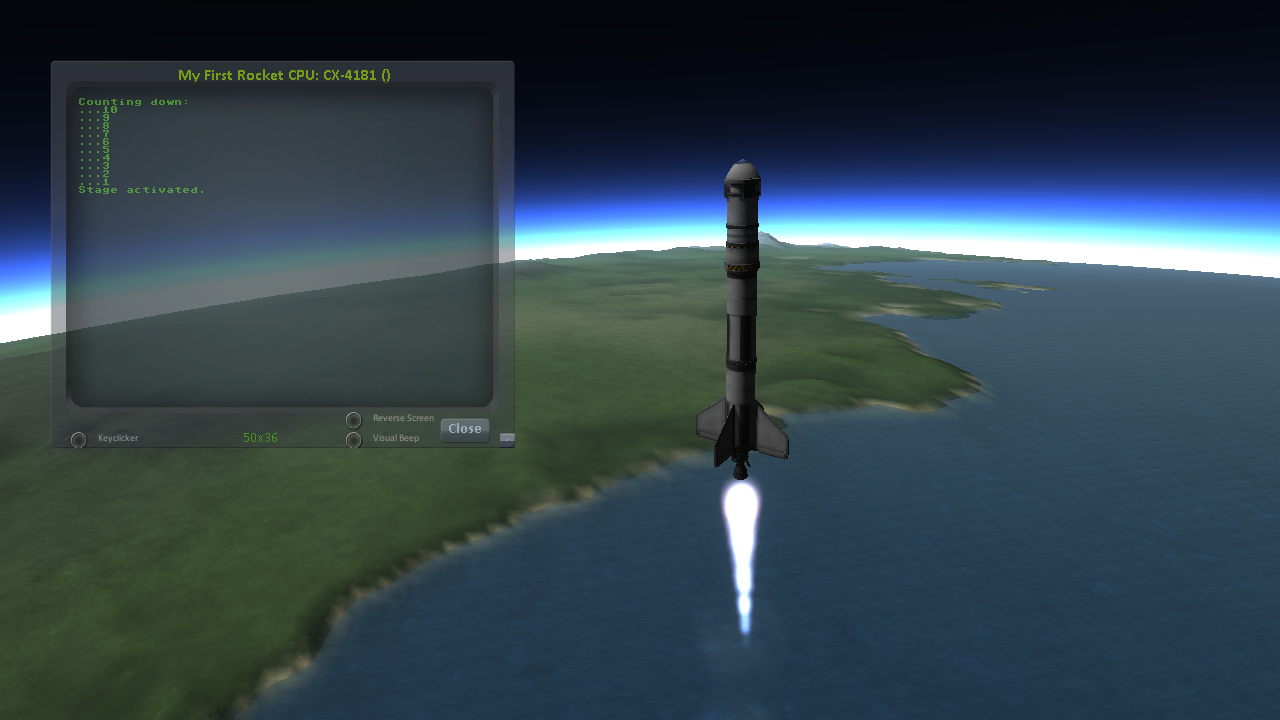
\includegraphics[width=0.800\linewidth]{example_2_3.png}
\end{figure}

Now you should see the same thing as before, but now your craft will stay pointed up.

\emph{But wait - it only does the first stage and then it stops without
doing the next stage? how do I fix that?}


\subsubsection{Step 5: Add staging logic}
\label{tutorials/quickstart:step-5-add-staging-logic}
The logic for how and when to stage can be an interesting and fun thing to write yourself. This example will keep it very simple, and this is the part where it's important that you are using a vessel that only contains liquidfuel engines. If your vessel has some booster engines, then it would require a more sophisticated script to launch it correctly than this tutorial gives you.

To add the logic to check when to stage, we introduce a new concept called the WHEN trigger. To see full documentation on it when you finish the tutorial, look for it on the Flow Control page

The quick and dirty explanation is that a WHEN section is a short section of code that you set up to run LATER rather than right now. It creates a check in the background that will constantly look for some condition to occur, and when it happens, it interrupts whatever else the code is doing, and it will run the body of the WHEN code before continuing from where it left off in the main script.

There are some complex dangers with writing WHEN triggers that can cause \textbf{KSP} itself to hang or stutter if you are not careful, but explaining them is beyond the scope of this tutorial. But when you want to start using WHEN triggers yourself, you really should read the section on WHEN in the Flow Control page before you do so.

The WHEN trigger we are going to add to the launch script looks like this:

\begin{Verbatim}[commandchars=\\\{\}]
\PYG{n}{WHEN} \PYG{n}{MAXTHRUST} \PYG{o}{=} \PYG{l+m+mi}{0} \PYG{n}{THEN} \PYG{p}{\PYGZob{}}
    \PYG{n}{PRINT} \PYG{l+s}{\PYGZdq{}}\PYG{l+s}{Staging}\PYG{l+s}{\PYGZdq{}}\PYG{p}{.}
    \PYG{n}{STAGE}\PYG{p}{.}
    \PYG{n}{PRESERVE}\PYG{p}{.}
\PYG{p}{\PYGZcb{}}\PYG{p}{.}
\end{Verbatim}

It says, ``Whenever the maximum thrust of our vehicle is zero, then activate the next stage.'' The PRESERVE keyword says, ``don't stop checking this condition just because it's been triggered once. It should still keep checking for it again in the future.''
If this block of code is inserted into the script, then it will set up a constant background check that will always hit the next stage as soon as the current stage has no thrust.
UNLIKE with all the previous edits this tutorial has asked you to make to the script, this time you're going to be asked to delete something and replace it. The new WHEN section above should actually \textbf{REPLACE} the existing ``UNTIL SHIP:MAXTHRUST \textgreater{} 0'' loop that you had before.

Now your script should look like this:

\begin{Verbatim}[commandchars=\\\{\}]
\PYG{c+c1}{//hellolaunch}

\PYG{c+c1}{//First, we\PYGZsq{}ll clear the terminal screen to make it look nice}
\PYG{n}{CLEARSCREEN}\PYG{p}{.}

\PYG{c+c1}{//Next, we\PYGZsq{}ll lock our throttle to 100\PYGZpc{}.}
\PYG{n}{LOCK} \PYG{n}{THROTTLE} \PYG{n}{TO} \PYG{l+m+mf}{1.0}\PYG{p}{.}   \PYG{c+c1}{// 1.0 is the max, 0.0 is idle.}

\PYG{c+c1}{//This is our countdown loop, which cycles from 10 to 0}
\PYG{n}{PRINT} \PYG{l+s}{\PYGZdq{}}\PYG{l+s}{Counting down:}\PYG{l+s}{\PYGZdq{}}\PYG{p}{.}
\PYG{n}{FROM} \PYG{p}{\PYGZob{}}\PYG{n}{local} \PYG{n}{countdown} \PYG{n}{is} \PYG{l+m+mf}{10.}\PYG{p}{\PYGZcb{}} \PYG{n}{UNTIL} \PYG{n}{countdown} \PYG{o}{=} \PYG{l+m+mi}{0} \PYG{n}{STEP} \PYG{p}{\PYGZob{}}\PYG{n}{SET} \PYG{n}{countdown} \PYG{n}{to} \PYG{n}{countdown} \PYG{o}{\PYGZhy{}} \PYG{l+m+mf}{1.}\PYG{p}{\PYGZcb{}} \PYG{n}{DO} \PYG{p}{\PYGZob{}}
    \PYG{n}{PRINT} \PYG{l+s}{\PYGZdq{}}\PYG{l+s}{...}\PYG{l+s}{\PYGZdq{}} \PYG{o}{+} \PYG{n}{countdown}\PYG{p}{.}
    \PYG{n}{WAIT} \PYG{l+m+mf}{1.} \PYG{c+c1}{// pauses the script here for 1 second.}
\PYG{p}{\PYGZcb{}}

\PYG{c+c1}{//This is a trigger that constantly checks to see if our thrust is zero.}
\PYG{c+c1}{//If it is, it will attempt to stage and then return to where the script}
\PYG{c+c1}{//left off. The PRESERVE keyword keeps the trigger active even after it}
\PYG{c+c1}{//has been triggered.}
\PYG{n}{WHEN} \PYG{n}{MAXTHRUST} \PYG{o}{=} \PYG{l+m+mi}{0} \PYG{n}{THEN} \PYG{p}{\PYGZob{}}
    \PYG{n}{PRINT} \PYG{l+s}{\PYGZdq{}}\PYG{l+s}{Staging}\PYG{l+s}{\PYGZdq{}}\PYG{p}{.}
    \PYG{n}{STAGE}\PYG{p}{.}
    \PYG{n}{PRESERVE}\PYG{p}{.}
\PYG{p}{\PYGZcb{}}\PYG{p}{.}

\PYG{n}{LOCK} \PYG{n}{STEERING} \PYG{n}{TO} \PYG{n}{UP}\PYG{p}{.}

\PYG{n}{WAIT} \PYG{n}{UNTIL} \PYG{n}{ALTITUDE} \PYG{o}{\PYGZgt{}} \PYG{l+m+mf}{70000.}

\PYG{c+c1}{// NOTE that it is vital to not just let the script end right away}
\PYG{c+c1}{// here.  Once a kOS script just ends, it releases all the controls}
\PYG{c+c1}{// back to manual piloting so that you can fly the ship by hand again.}
\PYG{c+c1}{// If the program just ended here, then that would cause the throttle}
\PYG{c+c1}{// to turn back off again right away and nothing would happen.}
\end{Verbatim}

Again, relaunch the ship, copy the script as before, and run it again. This time you should see it activate your later upper stages correctly.
\begin{figure}[htbp]
\centering

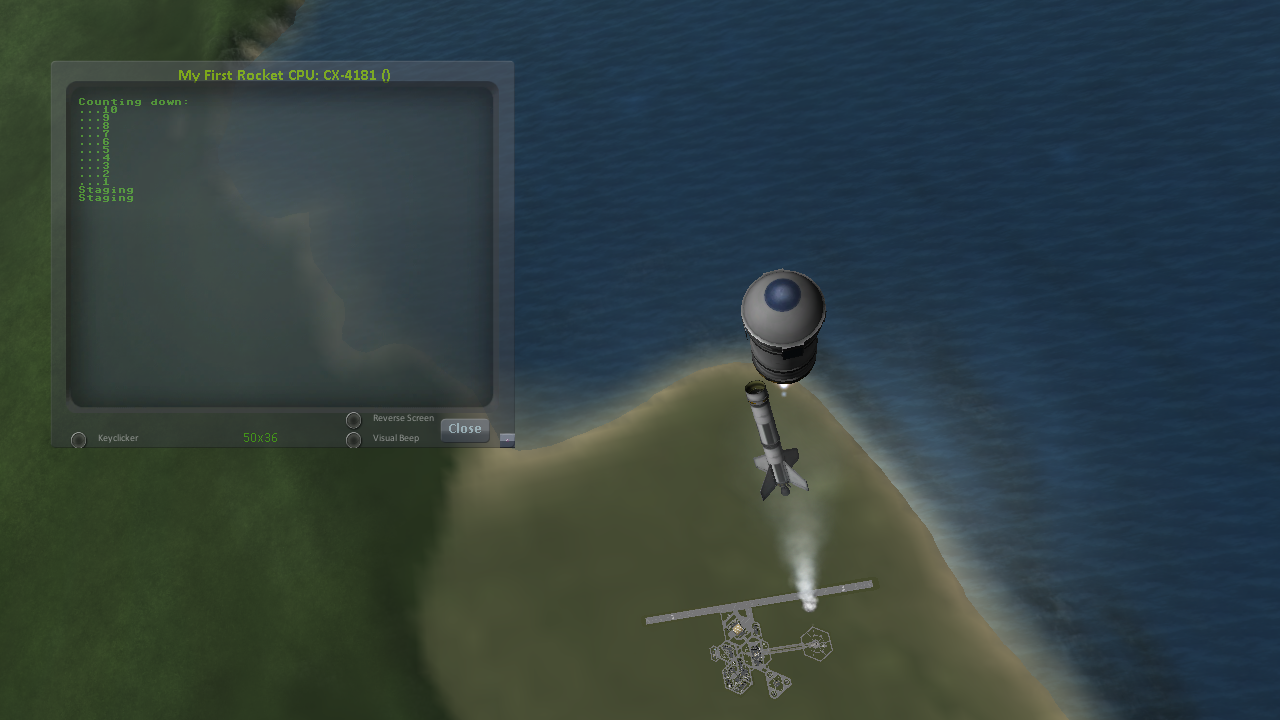
\includegraphics[width=0.800\linewidth]{example_2_4.png}
\end{figure}


\subsubsection{Step 6: Now to make it turn}
\label{tutorials/quickstart:step-6-now-to-make-it-turn}
\emph{Okay that's fine but it still just goes straight up! What about a
gravity turn?}

Well, a true and proper gravity turn is a very complex bit of math that is best left as an exercise for the reader, given that the goal of \textbf{kOS} is to let you write your OWN autopilot, not to write it for you. But to give some basic examples of commands, lets just make a crude gravity turn approximation that simply flies the ship like a lot of new \textbf{KSP} pilots learn to do it for the first time:
\begin{itemize}
\item {} 
Fly straight up until your velocity is 100m/s.

\item {} 
Pitch ten degrees towards the East.

\item {} 
Continue to pitch 10 degrees down for each 100m/s of velocity.

\end{itemize}

To make this work, we introduce a new way to make a Direction, called the HEADING function. Whenever you call the function HEADING(a,b), it makes a Direction oriented as follows on the navball:
\begin{itemize}
\item {} 
Point at the compass heading A.

\item {} 
Pitch up a number of degrees from the horizon = to B.

\end{itemize}

So for example, HEADING(45,10) would aim northeast, 10 degrees above the horizon. We can use this to easily set our orientation. For example:

\begin{Verbatim}[commandchars=\\\{\}]
\PYG{c+c1}{//This locks our steering to due east, pitched 45 degrees above the horizon.}
\PYG{n}{LOCK} \PYG{n}{STEERING} \PYG{n}{TO} \PYG{n}{HEADING}\PYG{p}{(}\PYG{l+m+mi}{90}\PYG{p}{,}\PYG{l+m+mi}{45}\PYG{p}{)}\PYG{p}{.}
\end{Verbatim}

Instead of using WAIT UNTIL to pause the script and keep it from exiting, we can use an UNTIL loop to constantly perform actions until a certain condition is met. For example:

\begin{Verbatim}[commandchars=\\\{\}]
\PYG{n}{UNTIL} \PYG{n}{APOAPSIS} \PYG{o}{\PYGZgt{}} \PYG{l+m+mi}{100000} \PYG{p}{\PYGZob{}}
    \PYG{n}{LOCK} \PYG{n}{STEERING} \PYG{n}{TO} \PYG{n}{HEADING}\PYG{p}{(}\PYG{l+m+mi}{90}\PYG{p}{,}\PYG{l+m+mi}{90}\PYG{p}{)}\PYG{p}{.} \PYG{c+c1}{//90 degrees east and pitched up 90 degrees (straight up)}
    \PYG{n}{PRINT} \PYG{n}{ROUND}\PYG{p}{(}\PYG{n+nl}{SHIP}\PYG{p}{:}\PYG{n}{APOAPSIS}\PYG{p}{,}\PYG{l+m+mi}{0}\PYG{p}{)} \PYG{n}{AT} \PYG{p}{(}\PYG{l+m+mi}{0}\PYG{p}{,}\PYG{l+m+mi}{16}\PYG{p}{)}\PYG{p}{.} \PYG{c+c1}{// prints new number, rounded to the nearest integer.}
    \PYG{c+c1}{//We use the PRINT AT() command here to keep from printing the same thing over and}
    \PYG{c+c1}{//over on a new line every time the loop iterates. Instead, this will always print}
    \PYG{c+c1}{//the apoapsis at the same point on the screen.}
\PYG{p}{\PYGZcb{}}\PYG{p}{.}
\end{Verbatim}

This loop will continue to execute all of its instructions until the apoapsis reaches 100km. Once the apoapsis is past 100km, the loop exits and the rest of the code continues.

We can combine this with IF statements in order to have one main loop that only executes certain chunks of its code under certain conditions. For example:

\begin{Verbatim}[commandchars=\\\{\}]
\PYG{n}{UNTIL} \PYG{n+nl}{SHIP}\PYG{p}{:}\PYG{n}{APOAPSIS} \PYG{o}{\PYGZgt{}} \PYG{l+m+mi}{100000} \PYG{p}{\PYGZob{}} \PYG{c+c1}{//Remember, all altitudes will be in meters, not kilometers}

    \PYG{c+c1}{//For the initial ascent, we want our steering to be straight}
    \PYG{c+c1}{//up and rolled due east}
    \PYG{n}{IF} \PYG{n+nl}{SHIP}\PYG{p}{:}\PYG{n+nl}{VELOCITY}\PYG{p}{:}\PYG{n+nl}{SURFACE}\PYG{p}{:}\PYG{n}{MAG} \PYG{o}{\PYGZlt{}} \PYG{l+m+mi}{100} \PYG{p}{\PYGZob{}}
        \PYG{c+c1}{//This sets our steering 90 degrees up and yawed to the compass}
        \PYG{c+c1}{//heading of 90 degrees (east)}
        \PYG{n}{LOCK} \PYG{n}{STEERING} \PYG{n}{TO} \PYG{n}{HEADING}\PYG{p}{(}\PYG{l+m+mi}{90}\PYG{p}{,}\PYG{l+m+mi}{90}\PYG{p}{)}\PYG{p}{.}

    \PYG{c+c1}{//Once we pass 100m/s, we want to pitch down ten degrees}
    \PYG{p}{\PYGZcb{}} \PYG{n}{ELSE} \PYG{n}{IF} \PYG{n+nl}{SHIP}\PYG{p}{:}\PYG{n+nl}{VELOCITY}\PYG{p}{:}\PYG{n+nl}{SURFACE}\PYG{p}{:}\PYG{n}{MAG} \PYG{o}{\PYGZgt{}}\PYG{o}{=} \PYG{l+m+mi}{100} \PYG{n}{AND} \PYG{n+nl}{SHIP}\PYG{p}{:}\PYG{n+nl}{VELOCITY}\PYG{p}{:}\PYG{n+nl}{SURFACE}\PYG{p}{:}\PYG{n}{MAG} \PYG{o}{\PYGZlt{}} \PYG{l+m+mi}{200} \PYG{p}{\PYGZob{}}
        \PYG{n}{LOCK} \PYG{n}{STEERING} \PYG{n}{TO} \PYG{n}{HEADING}\PYG{p}{(}\PYG{l+m+mi}{90}\PYG{p}{,}\PYG{l+m+mi}{80}\PYG{p}{)}\PYG{p}{.}
        \PYG{n}{PRINT} \PYG{l+s}{\PYGZdq{}}\PYG{l+s}{Pitching to 80 degrees}\PYG{l+s}{\PYGZdq{}} \PYG{n}{AT}\PYG{p}{(}\PYG{l+m+mi}{0}\PYG{p}{,}\PYG{l+m+mi}{15}\PYG{p}{)}\PYG{p}{.}
        \PYG{n}{PRINT} \PYG{n}{ROUND}\PYG{p}{(}\PYG{n+nl}{SHIP}\PYG{p}{:}\PYG{n}{APOAPSIS}\PYG{p}{,}\PYG{l+m+mi}{0}\PYG{p}{)} \PYG{n}{AT} \PYG{p}{(}\PYG{l+m+mi}{0}\PYG{p}{,}\PYG{l+m+mi}{16}\PYG{p}{)}\PYG{p}{.}
    \PYG{p}{\PYGZcb{}}\PYG{p}{.}
\PYG{p}{\PYGZcb{}}\PYG{p}{.}
\end{Verbatim}

Each time this loop iterates, it will check the surface velocity. If the velocity is below 100m/s, it will continuously execute the first block of instructions.
Once the velocity reaches 100m/s, it will stop executing the first block and start executing the second block, which will pitch the nose down to 80 degrees above the horizon.

Putting this into your script, it should look like this:

\begin{Verbatim}[commandchars=\\\{\}]
\PYG{c+c1}{//hellolaunch}

\PYG{c+c1}{//First, we\PYGZsq{}ll clear the terminal screen to make it look nice}
\PYG{n}{CLEARSCREEN}\PYG{p}{.}

\PYG{c+c1}{//Next, we\PYGZsq{}ll lock our throttle to 100\PYGZpc{}.}
\PYG{n}{LOCK} \PYG{n}{THROTTLE} \PYG{n}{TO} \PYG{l+m+mf}{1.0}\PYG{p}{.}   \PYG{c+c1}{// 1.0 is the max, 0.0 is idle.}

\PYG{c+c1}{//This is our countdown loop, which cycles from 10 to 0}
\PYG{n}{PRINT} \PYG{l+s}{\PYGZdq{}}\PYG{l+s}{Counting down:}\PYG{l+s}{\PYGZdq{}}\PYG{p}{.}
\PYG{n}{FROM} \PYG{p}{\PYGZob{}}\PYG{n}{local} \PYG{n}{countdown} \PYG{n}{is} \PYG{l+m+mf}{10.}\PYG{p}{\PYGZcb{}} \PYG{n}{UNTIL} \PYG{n}{countdown} \PYG{o}{=} \PYG{l+m+mi}{0} \PYG{n}{STEP} \PYG{p}{\PYGZob{}}\PYG{n}{SET} \PYG{n}{countdown} \PYG{n}{to} \PYG{n}{countdown} \PYG{o}{\PYGZhy{}} \PYG{l+m+mf}{1.}\PYG{p}{\PYGZcb{}} \PYG{n}{DO} \PYG{p}{\PYGZob{}}
    \PYG{n}{PRINT} \PYG{l+s}{\PYGZdq{}}\PYG{l+s}{...}\PYG{l+s}{\PYGZdq{}} \PYG{o}{+} \PYG{n}{countdown}\PYG{p}{.}
    \PYG{n}{WAIT} \PYG{l+m+mf}{1.} \PYG{c+c1}{// pauses the script here for 1 second.}
\PYG{p}{\PYGZcb{}}

\PYG{c+c1}{//This is a trigger that constantly checks to see if our thrust is zero.}
\PYG{c+c1}{//If it is, it will attempt to stage and then return to where the script}
\PYG{c+c1}{//left off. The PRESERVE keyword keeps the trigger active even after it}
\PYG{c+c1}{//has been triggered.}
\PYG{n}{WHEN} \PYG{n}{MAXTHRUST} \PYG{o}{=} \PYG{l+m+mi}{0} \PYG{n}{THEN} \PYG{p}{\PYGZob{}}
    \PYG{n}{PRINT} \PYG{l+s}{\PYGZdq{}}\PYG{l+s}{Staging}\PYG{l+s}{\PYGZdq{}}\PYG{p}{.}
    \PYG{n}{STAGE}\PYG{p}{.}
    \PYG{n}{PRESERVE}\PYG{p}{.}
\PYG{p}{\PYGZcb{}}\PYG{p}{.}

\PYG{c+c1}{//This will be our main control loop for the ascent. It will}
\PYG{c+c1}{//cycle through continuously until our apoapsis is greater}
\PYG{c+c1}{//than 100km. Each cycle, it will check each of the IF}
\PYG{c+c1}{//statements inside and perform them if their conditions}
\PYG{c+c1}{//are met}
\PYG{n}{UNTIL} \PYG{n+nl}{SHIP}\PYG{p}{:}\PYG{n}{APOAPSIS} \PYG{o}{\PYGZgt{}} \PYG{l+m+mi}{100000} \PYG{p}{\PYGZob{}} \PYG{c+c1}{//Remember, all altitudes will be in meters, not kilometers}

    \PYG{c+c1}{//For the initial ascent, we want our steering to be straight}
    \PYG{c+c1}{//up and rolled due east}
    \PYG{n}{IF} \PYG{n+nl}{SHIP}\PYG{p}{:}\PYG{n+nl}{VELOCITY}\PYG{p}{:}\PYG{n+nl}{SURFACE}\PYG{p}{:}\PYG{n}{MAG} \PYG{o}{\PYGZlt{}} \PYG{l+m+mi}{100} \PYG{p}{\PYGZob{}}
        \PYG{c+c1}{//This sets our steering 90 degrees up and yawed to the compass}
        \PYG{c+c1}{//heading of 90 degrees (east)}
        \PYG{n}{LOCK} \PYG{n}{STEERING} \PYG{n}{TO} \PYG{n}{HEADING}\PYG{p}{(}\PYG{l+m+mi}{90}\PYG{p}{,}\PYG{l+m+mi}{90}\PYG{p}{)}\PYG{p}{.}

    \PYG{c+c1}{//Once we pass 100m/s, we want to pitch down ten degrees}
    \PYG{p}{\PYGZcb{}} \PYG{n}{ELSE} \PYG{n}{IF} \PYG{n+nl}{SHIP}\PYG{p}{:}\PYG{n+nl}{VELOCITY}\PYG{p}{:}\PYG{n+nl}{SURFACE}\PYG{p}{:}\PYG{n}{MAG} \PYG{o}{\PYGZgt{}}\PYG{o}{=} \PYG{l+m+mi}{100} \PYG{p}{\PYGZob{}}
        \PYG{n}{LOCK} \PYG{n}{STEERING} \PYG{n}{TO} \PYG{n}{HEADING}\PYG{p}{(}\PYG{l+m+mi}{90}\PYG{p}{,}\PYG{l+m+mi}{80}\PYG{p}{)}\PYG{p}{.}
        \PYG{n}{PRINT} \PYG{l+s}{\PYGZdq{}}\PYG{l+s}{Pitching to 80 degrees}\PYG{l+s}{\PYGZdq{}} \PYG{n}{AT}\PYG{p}{(}\PYG{l+m+mi}{0}\PYG{p}{,}\PYG{l+m+mi}{15}\PYG{p}{)}\PYG{p}{.}
        \PYG{n}{PRINT} \PYG{n}{ROUND}\PYG{p}{(}\PYG{n+nl}{SHIP}\PYG{p}{:}\PYG{n}{APOAPSIS}\PYG{p}{,}\PYG{l+m+mi}{0}\PYG{p}{)} \PYG{n}{AT} \PYG{p}{(}\PYG{l+m+mi}{0}\PYG{p}{,}\PYG{l+m+mi}{16}\PYG{p}{)}\PYG{p}{.}
    \PYG{p}{\PYGZcb{}}\PYG{p}{.}
\PYG{p}{\PYGZcb{}}\PYG{p}{.}
\end{Verbatim}

Again, copy this into your script and run it. You should see your countdown occur, then it will launch. Once the ship passes 100m/s surface velocity, it will
pitch down to 80 degrees and continuously print the apoapsis until the apoapsis reaches 100km, staging if necessary. The script will then end.
\begin{figure}[htbp]
\centering

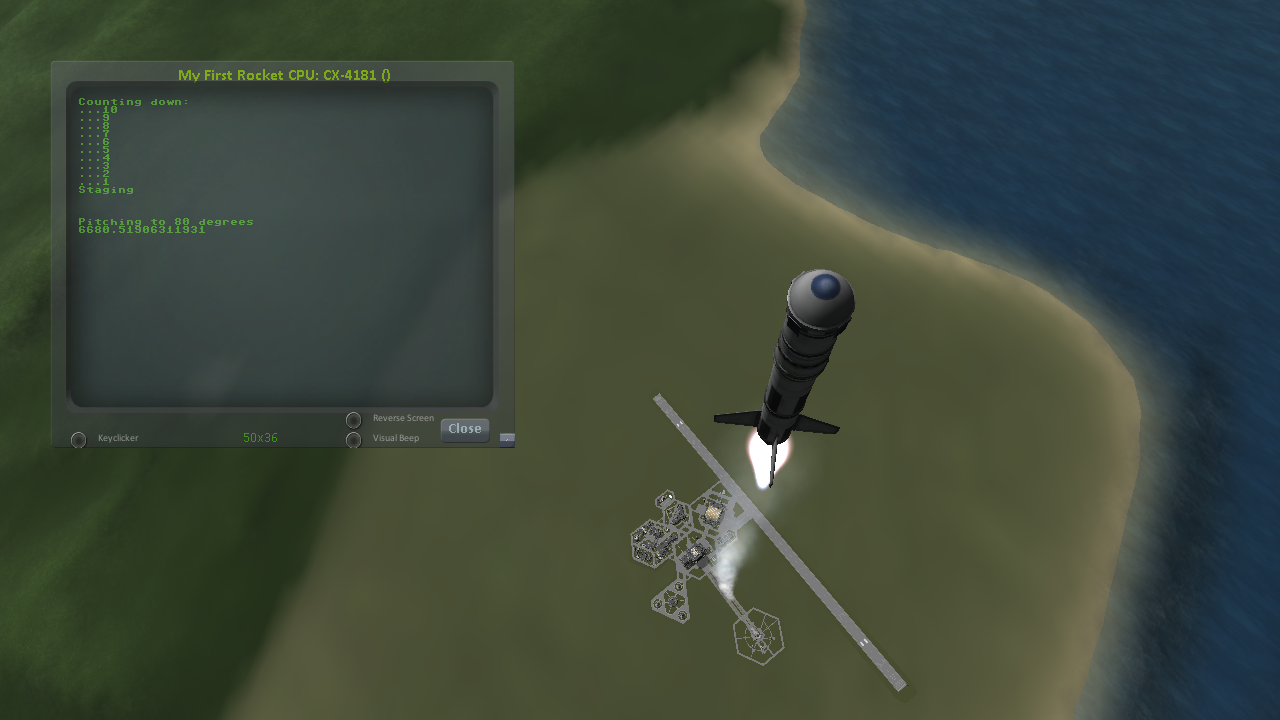
\includegraphics[width=0.800\linewidth]{example_2_5.png}
\end{figure}


\subsubsection{Step 7: Putting it all together}
\label{tutorials/quickstart:step-7-putting-it-all-together}
We now have every element of the script necessary to do a proper (albeit simple) gravity turn. We just need to extend it all the way through the ascent.

Adding additional IF statements inside our main loop will allow us to perform further actions based on our velocity. Each IF statement you see in the script below
covers a 100m/s block of velocity, and will adjust the pitch 10 degrees farther down than the previous block.

You can see that with the AND statement, we can check multiple conditions and only execute that block when all of those conditions are true. We can carefully set up
the conditions for each IF statement to allow a block of code to be executed no matter what our surface velocity is.

Copy this into your script and run it. It should take you nearly to orbit:

\begin{Verbatim}[commandchars=\\\{\}]
\PYG{c+c1}{//hellolaunch}

\PYG{c+c1}{//First, we\PYGZsq{}ll clear the terminal screen to make it look nice}
\PYG{n}{CLEARSCREEN}\PYG{p}{.}

\PYG{c+c1}{//Next, we\PYGZsq{}ll lock our throttle to 100\PYGZpc{}.}
\PYG{n}{LOCK} \PYG{n}{THROTTLE} \PYG{n}{TO} \PYG{l+m+mf}{1.0}\PYG{p}{.}   \PYG{c+c1}{// 1.0 is the max, 0.0 is idle.}

\PYG{c+c1}{//This is our countdown loop, which cycles from 10 to 0}
\PYG{n}{PRINT} \PYG{l+s}{\PYGZdq{}}\PYG{l+s}{Counting down:}\PYG{l+s}{\PYGZdq{}}\PYG{p}{.}
\PYG{n}{FROM} \PYG{p}{\PYGZob{}}\PYG{n}{local} \PYG{n}{countdown} \PYG{n}{is} \PYG{l+m+mf}{10.}\PYG{p}{\PYGZcb{}} \PYG{n}{UNTIL} \PYG{n}{countdown} \PYG{o}{=} \PYG{l+m+mi}{0} \PYG{n}{STEP} \PYG{p}{\PYGZob{}}\PYG{n}{SET} \PYG{n}{countdown} \PYG{n}{to} \PYG{n}{countdown} \PYG{o}{\PYGZhy{}} \PYG{l+m+mf}{1.}\PYG{p}{\PYGZcb{}} \PYG{n}{DO} \PYG{p}{\PYGZob{}}
    \PYG{n}{PRINT} \PYG{l+s}{\PYGZdq{}}\PYG{l+s}{...}\PYG{l+s}{\PYGZdq{}} \PYG{o}{+} \PYG{n}{countdown}\PYG{p}{.}
    \PYG{n}{WAIT} \PYG{l+m+mf}{1.} \PYG{c+c1}{// pauses the script here for 1 second.}
\PYG{p}{\PYGZcb{}}

\PYG{c+c1}{//This is a trigger that constantly checks to see if our thrust is zero.}
\PYG{c+c1}{//If it is, it will attempt to stage and then return to where the script}
\PYG{c+c1}{//left off. The PRESERVE keyword keeps the trigger active even after it}
\PYG{c+c1}{//has been triggered.}
\PYG{n}{WHEN} \PYG{n}{MAXTHRUST} \PYG{o}{=} \PYG{l+m+mi}{0} \PYG{n}{THEN} \PYG{p}{\PYGZob{}}
    \PYG{n}{PRINT} \PYG{l+s}{\PYGZdq{}}\PYG{l+s}{Staging}\PYG{l+s}{\PYGZdq{}}\PYG{p}{.}
    \PYG{n}{STAGE}\PYG{p}{.}
    \PYG{n}{PRESERVE}\PYG{p}{.}
\PYG{p}{\PYGZcb{}}\PYG{p}{.}

\PYG{c+c1}{//This will be our main control loop for the ascent. It will}
\PYG{c+c1}{//cycle through continuously until our apoapsis is greater}
\PYG{c+c1}{//than 100km. Each cycle, it will check each of the IF}
\PYG{c+c1}{//statements inside and perform them if their conditions}
\PYG{c+c1}{//are met}
\PYG{n}{UNTIL} \PYG{n+nl}{SHIP}\PYG{p}{:}\PYG{n}{APOAPSIS} \PYG{o}{\PYGZgt{}} \PYG{l+m+mi}{100000} \PYG{p}{\PYGZob{}} \PYG{c+c1}{//Remember, all altitudes will be in meters, not kilometers}

    \PYG{c+c1}{//For the initial ascent, we want our steering to be straight}
    \PYG{c+c1}{//up and rolled due east}
    \PYG{n}{IF} \PYG{n+nl}{SHIP}\PYG{p}{:}\PYG{n+nl}{VELOCITY}\PYG{p}{:}\PYG{n+nl}{SURFACE}\PYG{p}{:}\PYG{n}{MAG} \PYG{o}{\PYGZlt{}} \PYG{l+m+mi}{100} \PYG{p}{\PYGZob{}}
        \PYG{c+c1}{//This sets our steering 90 degrees up and yawed to the compass}
        \PYG{c+c1}{//heading of 90 degrees (east)}
        \PYG{n}{LOCK} \PYG{n}{STEERING} \PYG{n}{TO} \PYG{n}{HEADING}\PYG{p}{(}\PYG{l+m+mi}{90}\PYG{p}{,}\PYG{l+m+mi}{90}\PYG{p}{)}\PYG{p}{.}

    \PYG{c+c1}{//Once we pass 100m/s, we want to pitch down ten degrees}
    \PYG{p}{\PYGZcb{}} \PYG{n}{ELSE} \PYG{n}{IF} \PYG{n+nl}{SHIP}\PYG{p}{:}\PYG{n+nl}{VELOCITY}\PYG{p}{:}\PYG{n+nl}{SURFACE}\PYG{p}{:}\PYG{n}{MAG} \PYG{o}{\PYGZgt{}}\PYG{o}{=} \PYG{l+m+mi}{100} \PYG{n}{AND} \PYG{n+nl}{SHIP}\PYG{p}{:}\PYG{n+nl}{VELOCITY}\PYG{p}{:}\PYG{n+nl}{SURFACE}\PYG{p}{:}\PYG{n}{MAG} \PYG{o}{\PYGZlt{}} \PYG{l+m+mi}{200} \PYG{p}{\PYGZob{}}
        \PYG{n}{LOCK} \PYG{n}{STEERING} \PYG{n}{TO} \PYG{n}{HEADING}\PYG{p}{(}\PYG{l+m+mi}{90}\PYG{p}{,}\PYG{l+m+mi}{80}\PYG{p}{)}\PYG{p}{.}
        \PYG{n}{PRINT} \PYG{l+s}{\PYGZdq{}}\PYG{l+s}{Pitching to 80 degrees}\PYG{l+s}{\PYGZdq{}} \PYG{n}{AT}\PYG{p}{(}\PYG{l+m+mi}{0}\PYG{p}{,}\PYG{l+m+mi}{15}\PYG{p}{)}\PYG{p}{.}
        \PYG{n}{PRINT} \PYG{n}{ROUND}\PYG{p}{(}\PYG{n+nl}{SHIP}\PYG{p}{:}\PYG{n}{APOAPSIS}\PYG{p}{,}\PYG{l+m+mi}{0}\PYG{p}{)} \PYG{n}{AT} \PYG{p}{(}\PYG{l+m+mi}{0}\PYG{p}{,}\PYG{l+m+mi}{16}\PYG{p}{)}\PYG{p}{.}

    \PYG{c+c1}{//Each successive IF statement checks to see if our velocity}
    \PYG{c+c1}{//is within a 100m/s block and adjusts our heading down another}
    \PYG{c+c1}{//ten degrees if so}
    \PYG{p}{\PYGZcb{}} \PYG{n}{ELSE} \PYG{n}{IF} \PYG{n+nl}{SHIP}\PYG{p}{:}\PYG{n+nl}{VELOCITY}\PYG{p}{:}\PYG{n+nl}{SURFACE}\PYG{p}{:}\PYG{n}{MAG} \PYG{o}{\PYGZgt{}}\PYG{o}{=} \PYG{l+m+mi}{200} \PYG{n}{AND} \PYG{n+nl}{SHIP}\PYG{p}{:}\PYG{n+nl}{VELOCITY}\PYG{p}{:}\PYG{n+nl}{SURFACE}\PYG{p}{:}\PYG{n}{MAG} \PYG{o}{\PYGZlt{}} \PYG{l+m+mi}{300} \PYG{p}{\PYGZob{}}
        \PYG{n}{LOCK} \PYG{n}{STEERING} \PYG{n}{TO} \PYG{n}{HEADING}\PYG{p}{(}\PYG{l+m+mi}{90}\PYG{p}{,}\PYG{l+m+mi}{70}\PYG{p}{)}\PYG{p}{.}
        \PYG{n}{PRINT} \PYG{l+s}{\PYGZdq{}}\PYG{l+s}{Pitching to 70 degrees}\PYG{l+s}{\PYGZdq{}} \PYG{n}{AT}\PYG{p}{(}\PYG{l+m+mi}{0}\PYG{p}{,}\PYG{l+m+mi}{15}\PYG{p}{)}\PYG{p}{.}
        \PYG{n}{PRINT} \PYG{n}{ROUND}\PYG{p}{(}\PYG{n+nl}{SHIP}\PYG{p}{:}\PYG{n}{APOAPSIS}\PYG{p}{,}\PYG{l+m+mi}{0}\PYG{p}{)} \PYG{n}{AT} \PYG{p}{(}\PYG{l+m+mi}{0}\PYG{p}{,}\PYG{l+m+mi}{16}\PYG{p}{)}\PYG{p}{.}

    \PYG{p}{\PYGZcb{}} \PYG{n}{ELSE} \PYG{n}{IF} \PYG{n+nl}{SHIP}\PYG{p}{:}\PYG{n+nl}{VELOCITY}\PYG{p}{:}\PYG{n+nl}{SURFACE}\PYG{p}{:}\PYG{n}{MAG} \PYG{o}{\PYGZgt{}}\PYG{o}{=} \PYG{l+m+mi}{300} \PYG{n}{AND} \PYG{n+nl}{SHIP}\PYG{p}{:}\PYG{n+nl}{VELOCITY}\PYG{p}{:}\PYG{n+nl}{SURFACE}\PYG{p}{:}\PYG{n}{MAG} \PYG{o}{\PYGZlt{}} \PYG{l+m+mi}{400} \PYG{p}{\PYGZob{}}
        \PYG{n}{LOCK} \PYG{n}{STEERING} \PYG{n}{TO} \PYG{n}{HEADING}\PYG{p}{(}\PYG{l+m+mi}{90}\PYG{p}{,}\PYG{l+m+mi}{60}\PYG{p}{)}\PYG{p}{.}
        \PYG{n}{PRINT} \PYG{l+s}{\PYGZdq{}}\PYG{l+s}{Pitching to 60 degrees}\PYG{l+s}{\PYGZdq{}} \PYG{n}{AT}\PYG{p}{(}\PYG{l+m+mi}{0}\PYG{p}{,}\PYG{l+m+mi}{15}\PYG{p}{)}\PYG{p}{.}
        \PYG{n}{PRINT} \PYG{n}{ROUND}\PYG{p}{(}\PYG{n+nl}{SHIP}\PYG{p}{:}\PYG{n}{APOAPSIS}\PYG{p}{,}\PYG{l+m+mi}{0}\PYG{p}{)} \PYG{n}{AT} \PYG{p}{(}\PYG{l+m+mi}{0}\PYG{p}{,}\PYG{l+m+mi}{16}\PYG{p}{)}\PYG{p}{.}

    \PYG{p}{\PYGZcb{}} \PYG{n}{ELSE} \PYG{n}{IF} \PYG{n+nl}{SHIP}\PYG{p}{:}\PYG{n+nl}{VELOCITY}\PYG{p}{:}\PYG{n+nl}{SURFACE}\PYG{p}{:}\PYG{n}{MAG} \PYG{o}{\PYGZgt{}}\PYG{o}{=} \PYG{l+m+mi}{400} \PYG{n}{AND} \PYG{n+nl}{SHIP}\PYG{p}{:}\PYG{n+nl}{VELOCITY}\PYG{p}{:}\PYG{n+nl}{SURFACE}\PYG{p}{:}\PYG{n}{MAG} \PYG{o}{\PYGZlt{}} \PYG{l+m+mi}{500} \PYG{p}{\PYGZob{}}
        \PYG{n}{LOCK} \PYG{n}{STEERING} \PYG{n}{TO} \PYG{n}{HEADING}\PYG{p}{(}\PYG{l+m+mi}{90}\PYG{p}{,}\PYG{l+m+mi}{50}\PYG{p}{)}\PYG{p}{.}
        \PYG{n}{PRINT} \PYG{l+s}{\PYGZdq{}}\PYG{l+s}{Pitching to 50 degrees}\PYG{l+s}{\PYGZdq{}} \PYG{n}{AT}\PYG{p}{(}\PYG{l+m+mi}{0}\PYG{p}{,}\PYG{l+m+mi}{15}\PYG{p}{)}\PYG{p}{.}
        \PYG{n}{PRINT} \PYG{n}{ROUND}\PYG{p}{(}\PYG{n+nl}{SHIP}\PYG{p}{:}\PYG{n}{APOAPSIS}\PYG{p}{,}\PYG{l+m+mi}{0}\PYG{p}{)} \PYG{n}{AT} \PYG{p}{(}\PYG{l+m+mi}{0}\PYG{p}{,}\PYG{l+m+mi}{16}\PYG{p}{)}\PYG{p}{.}

    \PYG{p}{\PYGZcb{}} \PYG{n}{ELSE} \PYG{n}{IF} \PYG{n+nl}{SHIP}\PYG{p}{:}\PYG{n+nl}{VELOCITY}\PYG{p}{:}\PYG{n+nl}{SURFACE}\PYG{p}{:}\PYG{n}{MAG} \PYG{o}{\PYGZgt{}}\PYG{o}{=} \PYG{l+m+mi}{500} \PYG{n}{AND} \PYG{n+nl}{SHIP}\PYG{p}{:}\PYG{n+nl}{VELOCITY}\PYG{p}{:}\PYG{n+nl}{SURFACE}\PYG{p}{:}\PYG{n}{MAG} \PYG{o}{\PYGZlt{}} \PYG{l+m+mi}{600} \PYG{p}{\PYGZob{}}
        \PYG{n}{LOCK} \PYG{n}{STEERING} \PYG{n}{TO} \PYG{n}{HEADING}\PYG{p}{(}\PYG{l+m+mi}{90}\PYG{p}{,}\PYG{l+m+mi}{40}\PYG{p}{)}\PYG{p}{.}
        \PYG{n}{PRINT} \PYG{l+s}{\PYGZdq{}}\PYG{l+s}{Pitching to 40 degrees}\PYG{l+s}{\PYGZdq{}} \PYG{n}{AT}\PYG{p}{(}\PYG{l+m+mi}{0}\PYG{p}{,}\PYG{l+m+mi}{15}\PYG{p}{)}\PYG{p}{.}
        \PYG{n}{PRINT} \PYG{n}{ROUND}\PYG{p}{(}\PYG{n+nl}{SHIP}\PYG{p}{:}\PYG{n}{APOAPSIS}\PYG{p}{,}\PYG{l+m+mi}{0}\PYG{p}{)} \PYG{n}{AT} \PYG{p}{(}\PYG{l+m+mi}{0}\PYG{p}{,}\PYG{l+m+mi}{16}\PYG{p}{)}\PYG{p}{.}

    \PYG{p}{\PYGZcb{}} \PYG{n}{ELSE} \PYG{n}{IF} \PYG{n+nl}{SHIP}\PYG{p}{:}\PYG{n+nl}{VELOCITY}\PYG{p}{:}\PYG{n+nl}{SURFACE}\PYG{p}{:}\PYG{n}{MAG} \PYG{o}{\PYGZgt{}}\PYG{o}{=} \PYG{l+m+mi}{600} \PYG{n}{AND} \PYG{n+nl}{SHIP}\PYG{p}{:}\PYG{n+nl}{VELOCITY}\PYG{p}{:}\PYG{n+nl}{SURFACE}\PYG{p}{:}\PYG{n}{MAG} \PYG{o}{\PYGZlt{}} \PYG{l+m+mi}{700} \PYG{p}{\PYGZob{}}
        \PYG{n}{LOCK} \PYG{n}{STEERING} \PYG{n}{TO} \PYG{n}{HEADING}\PYG{p}{(}\PYG{l+m+mi}{90}\PYG{p}{,}\PYG{l+m+mi}{30}\PYG{p}{)}\PYG{p}{.}
        \PYG{n}{PRINT} \PYG{l+s}{\PYGZdq{}}\PYG{l+s}{Pitching to 30 degrees}\PYG{l+s}{\PYGZdq{}} \PYG{n}{AT}\PYG{p}{(}\PYG{l+m+mi}{0}\PYG{p}{,}\PYG{l+m+mi}{15}\PYG{p}{)}\PYG{p}{.}
        \PYG{n}{PRINT} \PYG{n}{ROUND}\PYG{p}{(}\PYG{n+nl}{SHIP}\PYG{p}{:}\PYG{n}{APOAPSIS}\PYG{p}{,}\PYG{l+m+mi}{0}\PYG{p}{)} \PYG{n}{AT} \PYG{p}{(}\PYG{l+m+mi}{0}\PYG{p}{,}\PYG{l+m+mi}{16}\PYG{p}{)}\PYG{p}{.}

    \PYG{p}{\PYGZcb{}} \PYG{n}{ELSE} \PYG{n}{IF} \PYG{n+nl}{SHIP}\PYG{p}{:}\PYG{n+nl}{VELOCITY}\PYG{p}{:}\PYG{n+nl}{SURFACE}\PYG{p}{:}\PYG{n}{MAG} \PYG{o}{\PYGZgt{}}\PYG{o}{=} \PYG{l+m+mi}{700} \PYG{n}{AND} \PYG{n+nl}{SHIP}\PYG{p}{:}\PYG{n+nl}{VELOCITY}\PYG{p}{:}\PYG{n+nl}{SURFACE}\PYG{p}{:}\PYG{n}{MAG} \PYG{o}{\PYGZlt{}} \PYG{l+m+mi}{800} \PYG{p}{\PYGZob{}}
        \PYG{n}{LOCK} \PYG{n}{STEERING} \PYG{n}{TO} \PYG{n}{HEADING}\PYG{p}{(}\PYG{l+m+mi}{90}\PYG{p}{,}\PYG{l+m+mi}{11}\PYG{p}{)}\PYG{p}{.}
        \PYG{n}{PRINT} \PYG{l+s}{\PYGZdq{}}\PYG{l+s}{Pitching to 20 degrees}\PYG{l+s}{\PYGZdq{}} \PYG{n}{AT}\PYG{p}{(}\PYG{l+m+mi}{0}\PYG{p}{,}\PYG{l+m+mi}{15}\PYG{p}{)}\PYG{p}{.}
        \PYG{n}{PRINT} \PYG{n}{ROUND}\PYG{p}{(}\PYG{n+nl}{SHIP}\PYG{p}{:}\PYG{n}{APOAPSIS}\PYG{p}{,}\PYG{l+m+mi}{0}\PYG{p}{)} \PYG{n}{AT} \PYG{p}{(}\PYG{l+m+mi}{0}\PYG{p}{,}\PYG{l+m+mi}{16}\PYG{p}{)}\PYG{p}{.}

    \PYG{c+c1}{//Beyond 800m/s, we can keep facing towards 10 degrees above the horizon and wait}
    \PYG{c+c1}{//for the main loop to recognize that our apoapsis is above 100km}
    \PYG{p}{\PYGZcb{}} \PYG{n}{ELSE} \PYG{n}{IF} \PYG{n+nl}{SHIP}\PYG{p}{:}\PYG{n+nl}{VELOCITY}\PYG{p}{:}\PYG{n+nl}{SURFACE}\PYG{p}{:}\PYG{n}{MAG} \PYG{o}{\PYGZgt{}}\PYG{o}{=} \PYG{l+m+mi}{800} \PYG{p}{\PYGZob{}}
        \PYG{n}{LOCK} \PYG{n}{STEERING} \PYG{n}{TO} \PYG{n}{HEADING}\PYG{p}{(}\PYG{l+m+mi}{90}\PYG{p}{,}\PYG{l+m+mi}{10}\PYG{p}{)}\PYG{p}{.}
        \PYG{n}{PRINT} \PYG{l+s}{\PYGZdq{}}\PYG{l+s}{Pitching to 10 degrees}\PYG{l+s}{\PYGZdq{}} \PYG{n}{AT}\PYG{p}{(}\PYG{l+m+mi}{0}\PYG{p}{,}\PYG{l+m+mi}{15}\PYG{p}{)}\PYG{p}{.}
        \PYG{n}{PRINT} \PYG{n}{ROUND}\PYG{p}{(}\PYG{n+nl}{SHIP}\PYG{p}{:}\PYG{n}{APOAPSIS}\PYG{p}{,}\PYG{l+m+mi}{0}\PYG{p}{)} \PYG{n}{AT} \PYG{p}{(}\PYG{l+m+mi}{0}\PYG{p}{,}\PYG{l+m+mi}{16}\PYG{p}{)}\PYG{p}{.}

    \PYG{p}{\PYGZcb{}}\PYG{p}{.}

\PYG{p}{\PYGZcb{}}\PYG{p}{.}

\PYG{n}{PRINT} \PYG{l+s}{\PYGZdq{}}\PYG{l+s}{100km apoapsis reached, cutting throttle}\PYG{l+s}{\PYGZdq{}}\PYG{p}{.}

\PYG{c+c1}{//At this point, our apoapsis is above 100km and our main loop has ended. Next}
\PYG{c+c1}{//we\PYGZsq{}ll make sure our throttle is zero and that we\PYGZsq{}re pointed prograde}
\PYG{n}{LOCK} \PYG{n}{THROTTLE} \PYG{n}{TO} \PYG{l+m+mf}{0.}

\PYG{c+c1}{//This sets the user\PYGZsq{}s throttle setting to zero to prevent the throttle}
\PYG{c+c1}{//from returning to the position it was at before the script was run.}
\PYG{n}{SET} \PYG{n+nl}{SHIP}\PYG{p}{:}\PYG{n+nl}{CONTROL}\PYG{p}{:}\PYG{n}{PILOTMAINTHROTTLE} \PYG{n}{TO} \PYG{l+m+mf}{0.}
\end{Verbatim}

And here is it in action:
\begin{figure}[htbp]
\centering

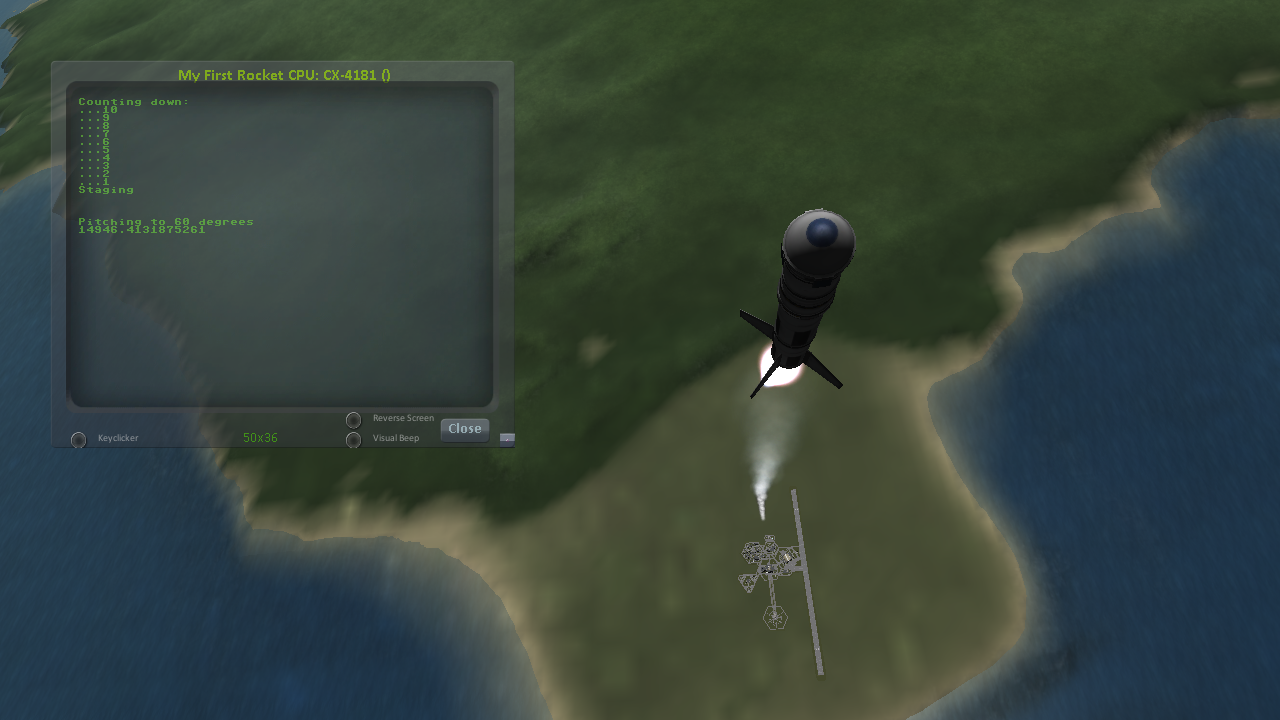
\includegraphics[width=0.800\linewidth]{example_2_6.png}
\end{figure}

And toward the end:
\begin{figure}[htbp]
\centering

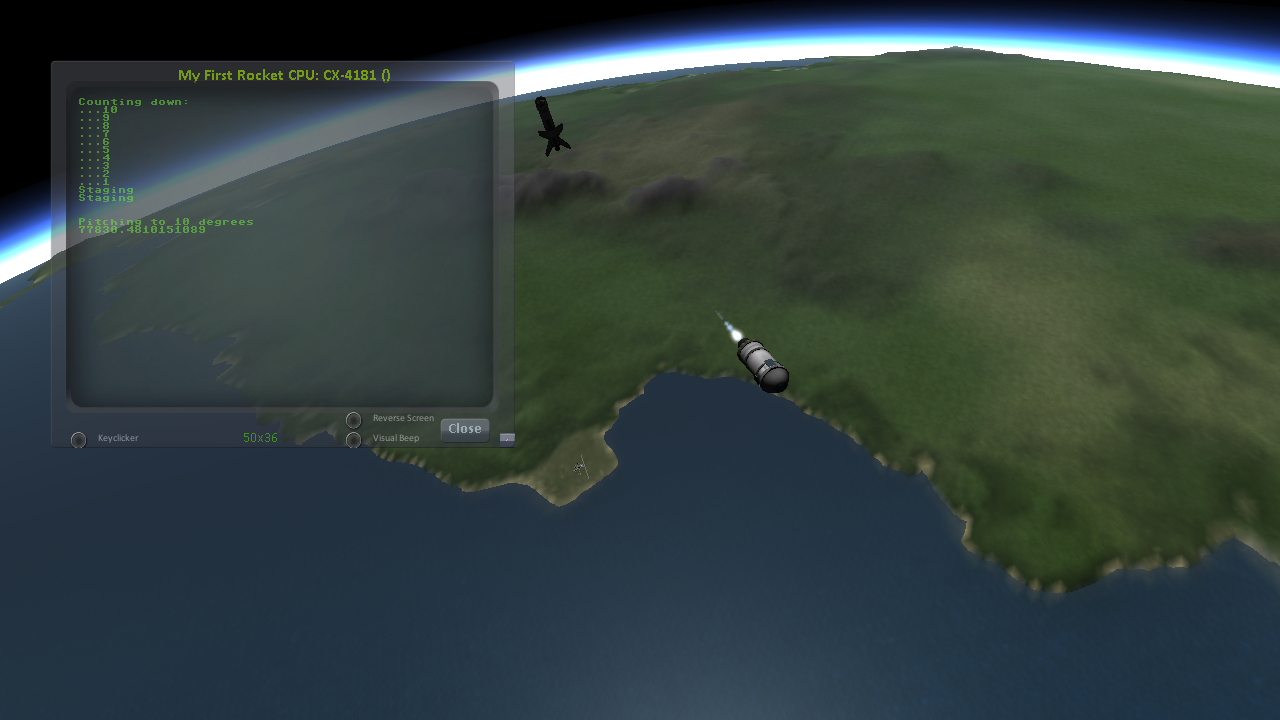
\includegraphics[width=0.800\linewidth]{example_2_7.png}
\end{figure}

This script should, in principle, work to get you to the point of leaving the atmosphere. It will probably still fall back down, because this script makes no attempt to ensure that the craft is going fast enough to maintain the orbit.

As you can probably see, it would still have a long way to go before it would become a really GOOD launching autopilot. Think about the following features you could add yourself as you become more familiar with \textbf{kOS}:
\begin{itemize}
\item {} 
You could change the steering logic to make a more smooth gravity turn by constantly adjusting the pitch in the HEADING according to some math formula. The example shown here tends to create a ``too high'' launch that's a bit inefficient. In addition, this method relies on velocity to determine pitch angle, which could result in some very firey launches for other ships with a higher TWR profile.

\item {} 
This script just stupidly leaves the throttle at max the whole way. You could make it more sophisticated by adjusting the throttle as necessary to avoid velocities that result in high atmospheric heating.

\item {} 
This script does not attempt to circularize. With some simple checks of the time to apoapsis and the orbital velocity, you can execute a burn that circularizes your orbit.

\item {} 
With even more sophisticated checks, the script could be made to work with fancy staging methods like asaparagus.

\item {} 
Using the PRINT AT command, you can make fancier status readouts in the terminal window as the script runs.

\end{itemize}


\section{Design Patterns and Considerations with kOS}
\label{tutorials/designpatterns:design-patterns-and-considerations-with-kos}\label{tutorials/designpatterns:designpatterns}\label{tutorials/designpatterns::doc}
There are many ways one can write a control program for a given scenario. The goal of this section is to help a novice kOS programmer, after having finished the {\hyperref[tutorials/quickstart:quickstart]{\emph{\DUspan{}{Quick Start Tutorial}}}}, to develop a sense of elegance and capability when writing his or her own kOS scripts. All of the examples in this tutorial may be tested by the reader using a rocket design similar to the following. Notice it carries an \href{http://wiki.kerbalspaceprogram.com/wiki/Double-C\_Seismic\_Accelerometer}{accelerometer} and the \href{http://wiki.kerbalspaceprogram.com/wiki/GRAVMAX\_Negative\_Gravioli\_Detector}{negative gravioli detector} which are used in the second section. Don't forget the kOS module as well!
\begin{figure}[htbp]
\centering

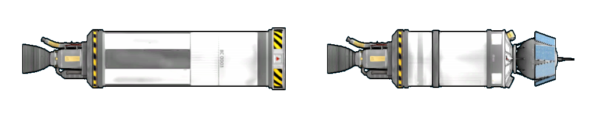
\includegraphics{designpatterns_rocket.png}
\label{tutorials/designpatterns:negative-gravioli-detector}\end{figure}
\setbox0\vbox{
\begin{minipage}{0.95\linewidth}
\textbf{Contents}

\medskip

\begin{itemize}
\item {} 
\phantomsection\label{tutorials/designpatterns:id1}{\hyperref[tutorials/designpatterns:the-major-design-patterns-of-kos-control-programs]{\emph{The Major Design Patterns of kOS Control Programs}}}
\begin{itemize}
\item {} 
\phantomsection\label{tutorials/designpatterns:id2}{\hyperref[tutorials/designpatterns:sequential-programs]{\emph{1. Sequential Programs}}}

\item {} 
\phantomsection\label{tutorials/designpatterns:id3}{\hyperref[tutorials/designpatterns:loops-with-condition-checking]{\emph{2. Loops with Condition Checking}}}

\item {} 
\phantomsection\label{tutorials/designpatterns:id4}{\hyperref[tutorials/designpatterns:loops-with-triggers]{\emph{3. Loops with Triggers}}}

\item {} 
\phantomsection\label{tutorials/designpatterns:id5}{\hyperref[tutorials/designpatterns:bringing-it-all-together]{\emph{Bringing It All Together}}}

\end{itemize}

\item {} 
\phantomsection\label{tutorials/designpatterns:id6}{\hyperref[tutorials/designpatterns:general-guidelines-for-kos-scripts]{\emph{General Guidelines for kOS Scripts}}}
\begin{itemize}
\item {} 
\phantomsection\label{tutorials/designpatterns:id7}{\hyperref[tutorials/designpatterns:minimize-time-spent-in-when-then-blocks]{\emph{1. Minimize Time Spent in WHEN/THEN Blocks}}}

\item {} 
\phantomsection\label{tutorials/designpatterns:id8}{\hyperref[tutorials/designpatterns:minimize-trigger-conditions]{\emph{2. Minimize Trigger Conditions}}}

\end{itemize}

\end{itemize}
\end{minipage}}
\begin{center}\setlength{\fboxsep}{5pt}\shadowbox{\box0}\end{center}


\subsection{The Major Design Patterns of kOS Control Programs}
\label{tutorials/designpatterns:the-major-design-patterns-of-kos-control-programs}
The design of a program is usually determined by the flow-control statements used. I.e., the WHEN/THEN, ON, WAIT, UNTIL, IF and FOR constructs. Here is a list of the major styles of control programs that can be written in kOS:
\begin{enumerate}
\item {} 
Sequential

\item {} 
Loops with Condition Checking

\item {} 
Loops with Triggers

\end{enumerate}

Of course, one style does not fit all scenarios and the programmer will typically want to use a combination of these all at once. Also, there may be other design patterns not listed here which can be perfectly valid, but this is a start.


\subsubsection{1. Sequential Programs}
\label{tutorials/designpatterns:sequential-programs}
These are programs that rely almost exclusively on WAIT UNTIL statements to go from one phase to the next.

\begin{Verbatim}[commandchars=\\\{\}]
\PYG{n}{LOCK} \PYG{n}{STEERING} \PYG{n}{TO} \PYG{n}{HEADING}\PYG{p}{(}\PYG{l+m+mi}{0}\PYG{p}{,}\PYG{l+m+mi}{90}\PYG{p}{)}\PYG{p}{.}
\PYG{n}{LOCK} \PYG{n}{THROTTLE} \PYG{n}{TO} \PYG{l+m+mf}{1.}
\PYG{n}{STAGE}\PYG{p}{.}
\PYG{n}{WAIT} \PYG{n}{UNTIL} \PYG{n+nl}{SHIP}\PYG{p}{:}\PYG{n}{ALTITUDE} \PYG{o}{\PYGZgt{}} \PYG{l+m+mf}{10000.}
\PYG{n}{LOCK} \PYG{n}{STEERING} \PYG{n}{TO} \PYG{n}{HEADING}\PYG{p}{(}\PYG{l+m+mi}{0}\PYG{p}{,}\PYG{l+m+mi}{90}\PYG{p}{)} \PYG{o}{+} \PYG{n}{R}\PYG{p}{(}\PYG{l+m+mi}{0}\PYG{p}{,}\PYG{o}{\PYGZhy{}}\PYG{l+m+mi}{45}\PYG{p}{,}\PYG{l+m+mi}{0}\PYG{p}{)}\PYG{p}{.}
\PYG{n}{WAIT} \PYG{n}{UNTIL} \PYG{n+nl}{STAGE}\PYG{p}{:}\PYG{n}{LIQUIDFUEL} \PYG{o}{\PYGZlt{}} \PYG{l+m+mf}{0.1}\PYG{p}{.}
\PYG{n}{STAGE}\PYG{p}{.}
\PYG{n}{WAIT} \PYG{n}{UNTIL} \PYG{n+nl}{SHIP}\PYG{p}{:}\PYG{n}{ALTITUDE} \PYG{o}{\PYGZgt{}} \PYG{l+m+mf}{20000.}
\PYG{n}{LOCK} \PYG{n}{THROTTLE} \PYG{n}{TO} \PYG{l+m+mf}{0.}
\PYG{n}{WAIT} \PYG{n}{UNTIL} \PYG{n}{FALSE}\PYG{p}{.} \PYG{c+c1}{// CTRL+C to break out}
\end{Verbatim}

This example will take a two stage rocket up to 20km. The immediate thing to notice is that the programmer must have known that the first stage would cutoff between 10km and 20km. This is fine for a specific rocket but not too general and could end in disaster if the first stage cutoff occurs at say 5km. Certainly, one can write a program using this technique to take a specific rocket, put it into orbit and even perform a lot of fancy maneuvers, but adapting the code to different rockets may get complicated quickly.


\subsubsection{2. Loops with Condition Checking}
\label{tutorials/designpatterns:loops-with-condition-checking}
Here, we introduce IF/ELSE logic into UNTIL loops:

\begin{Verbatim}[commandchars=\\\{\}]
\PYG{n}{LOCK} \PYG{n}{STEERING} \PYG{n}{TO} \PYG{n}{R}\PYG{p}{(}\PYG{l+m+mi}{0}\PYG{p}{,}\PYG{l+m+mi}{0}\PYG{p}{,}\PYG{o}{\PYGZhy{}}\PYG{l+m+mi}{90}\PYG{p}{)} \PYG{o}{+} \PYG{n}{HEADING}\PYG{p}{(}\PYG{l+m+mi}{90}\PYG{p}{,}\PYG{l+m+mi}{90}\PYG{p}{)}\PYG{p}{.}
\PYG{n}{LOCK} \PYG{n}{THROTTLE} \PYG{n}{TO} \PYG{l+m+mf}{1.}
\PYG{n}{STAGE}\PYG{p}{.}
\PYG{n}{UNTIL} \PYG{n+nl}{SHIP}\PYG{p}{:}\PYG{n}{ALTITUDE} \PYG{o}{\PYGZgt{}} \PYG{l+m+mi}{20000} \PYG{p}{\PYGZob{}}
    \PYG{n}{IF} \PYG{n+nl}{SHIP}\PYG{p}{:}\PYG{n}{ALTITUDE} \PYG{o}{\PYGZgt{}} \PYG{l+m+mi}{10000} \PYG{p}{\PYGZob{}}
        \PYG{n}{LOCK} \PYG{n}{STEERING} \PYG{n}{TO} \PYG{n}{R}\PYG{p}{(}\PYG{l+m+mi}{0}\PYG{p}{,}\PYG{l+m+mi}{0}\PYG{p}{,}\PYG{o}{\PYGZhy{}}\PYG{l+m+mi}{90}\PYG{p}{)} \PYG{o}{+} \PYG{n}{HEADING}\PYG{p}{(}\PYG{l+m+mi}{90}\PYG{p}{,}\PYG{l+m+mi}{45}\PYG{p}{)}\PYG{p}{.}
    \PYG{p}{\PYGZcb{}}
    \PYG{n}{IF} \PYG{n+nl}{STAGE}\PYG{p}{:}\PYG{n}{LIQUIDFUEL} \PYG{o}{\PYGZlt{}} \PYG{l+m+mf}{0.1} \PYG{p}{\PYGZob{}}
        \PYG{n}{STAGE}\PYG{p}{.}
    \PYG{p}{\PYGZcb{}}
\PYG{p}{\PYGZcb{}}
\PYG{n}{LOCK} \PYG{n}{THROTTLE} \PYG{n}{TO} \PYG{l+m+mf}{0.}
\PYG{n}{WAIT} \PYG{n}{UNTIL} \PYG{n}{FALSE}\PYG{p}{.}
\end{Verbatim}

This does the same thing as the previous example, but now it's checking for a staging condition from the launch pad all the way to 20km. More than that, it will stage as many times as needed.

One can imagine that these types of UNTIL loops can become very complex with many layers of IF/ELSE blocks. Once this happens it is usually good to reduce the frequency of the loop by adding a WAIT statement at the end of the loop. This wait could be anywhere from 0.001 (every physics tick), to 60 (every minute) or even longer for inter-planetary transfers if desired.


\subsubsection{3. Loops with Triggers}
\label{tutorials/designpatterns:loops-with-triggers}
In the above example, once the rocket reaches 10km, the steering is constantly being re-locked to HEADING(90,45). This works, but it only needs to be locked once. A possible improvement is to set up a trigger using a WHEN/THEN statement:

\begin{Verbatim}[commandchars=\\\{\}]
\PYG{n}{LOCK} \PYG{n}{STEERING} \PYG{n}{TO} \PYG{n}{R}\PYG{p}{(}\PYG{l+m+mi}{0}\PYG{p}{,}\PYG{l+m+mi}{0}\PYG{p}{,}\PYG{o}{\PYGZhy{}}\PYG{l+m+mi}{90}\PYG{p}{)} \PYG{o}{+} \PYG{n}{HEADING}\PYG{p}{(}\PYG{l+m+mi}{90}\PYG{p}{,}\PYG{l+m+mi}{90}\PYG{p}{)}\PYG{p}{.}
\PYG{n}{LOCK} \PYG{n}{THROTTLE} \PYG{n}{TO} \PYG{l+m+mf}{1.}
\PYG{n}{STAGE}\PYG{p}{.}
\PYG{n}{WHEN} \PYG{n+nl}{SHIP}\PYG{p}{:}\PYG{n}{ALTITUDE} \PYG{o}{\PYGZgt{}} \PYG{l+m+mi}{10000} \PYG{n}{THEN} \PYG{p}{\PYGZob{}}
    \PYG{n}{LOCK} \PYG{n}{STEERING} \PYG{n}{TO} \PYG{n}{R}\PYG{p}{(}\PYG{l+m+mi}{0}\PYG{p}{,}\PYG{l+m+mi}{0}\PYG{p}{,}\PYG{o}{\PYGZhy{}}\PYG{l+m+mi}{90}\PYG{p}{)} \PYG{o}{+} \PYG{n}{HEADING}\PYG{p}{(}\PYG{l+m+mi}{90}\PYG{p}{,}\PYG{l+m+mi}{45}\PYG{p}{)}\PYG{p}{.}
\PYG{p}{\PYGZcb{}}
\PYG{n}{UNTIL} \PYG{n+nl}{SHIP}\PYG{p}{:}\PYG{n}{ALTITUDE} \PYG{o}{\PYGZgt{}} \PYG{l+m+mi}{20000} \PYG{p}{\PYGZob{}}
    \PYG{n}{IF} \PYG{n+nl}{STAGE}\PYG{p}{:}\PYG{n}{LIQUIDFUEL} \PYG{o}{\PYGZlt{}} \PYG{l+m+mf}{0.1} \PYG{p}{\PYGZob{}}
        \PYG{n}{STAGE}\PYG{p}{.}
    \PYG{p}{\PYGZcb{}}
\PYG{p}{\PYGZcb{}}
\PYG{n}{LOCK} \PYG{n}{THROTTLE} \PYG{n}{TO} \PYG{l+m+mf}{0.}
\PYG{n}{WAIT} \PYG{n}{UNTIL} \PYG{n}{FALSE}\PYG{p}{.}
\end{Verbatim}

Now, when the rocket reaches 10km, the steering is set once and the trigger is removed from the active list of triggers. The staging condition can also be promoted to a trigger, keeping the trigger active after every stage using the PRESERVE keyword:

\begin{Verbatim}[commandchars=\\\{\}]
\PYG{n}{WHEN} \PYG{n+nl}{STAGE}\PYG{p}{:}\PYG{n}{LIQUIDFUEL} \PYG{o}{\PYGZlt{}} \PYG{l+m+mf}{0.1} \PYG{n}{THEN} \PYG{p}{\PYGZob{}}
    \PYG{n}{STAGE}\PYG{p}{.}
    \PYG{n}{PRESERVE}\PYG{p}{.}
\PYG{p}{\PYGZcb{}}
\PYG{n}{LOCK} \PYG{n}{STEERING} \PYG{n}{TO} \PYG{n}{R}\PYG{p}{(}\PYG{l+m+mi}{0}\PYG{p}{,}\PYG{l+m+mi}{0}\PYG{p}{,}\PYG{o}{\PYGZhy{}}\PYG{l+m+mi}{90}\PYG{p}{)} \PYG{o}{+} \PYG{n}{HEADING}\PYG{p}{(}\PYG{l+m+mi}{90}\PYG{p}{,}\PYG{l+m+mi}{90}\PYG{p}{)}\PYG{p}{.}
\PYG{n}{LOCK} \PYG{n}{THROTTLE} \PYG{n}{TO} \PYG{l+m+mf}{1.}
\PYG{n}{STAGE}\PYG{p}{.}
\PYG{n}{WHEN} \PYG{n+nl}{SHIP}\PYG{p}{:}\PYG{n}{ALTITUDE} \PYG{o}{\PYGZgt{}} \PYG{l+m+mi}{10000} \PYG{n}{THEN} \PYG{p}{\PYGZob{}}
    \PYG{n}{LOCK} \PYG{n}{STEERING} \PYG{n}{TO} \PYG{n}{R}\PYG{p}{(}\PYG{l+m+mi}{0}\PYG{p}{,}\PYG{l+m+mi}{0}\PYG{p}{,}\PYG{o}{\PYGZhy{}}\PYG{l+m+mi}{90}\PYG{p}{)} \PYG{o}{+} \PYG{n}{HEADING}\PYG{p}{(}\PYG{l+m+mi}{90}\PYG{p}{,}\PYG{l+m+mi}{45}\PYG{p}{)}\PYG{p}{.}
\PYG{p}{\PYGZcb{}}
\PYG{n}{WAIT} \PYG{n}{UNTIL} \PYG{n+nl}{SHIP}\PYG{p}{:}\PYG{n}{ALTITUDE} \PYG{o}{\PYGZgt{}} \PYG{l+m+mf}{20000.}
\PYG{n}{LOCK} \PYG{n}{THROTTLE} \PYG{n}{TO} \PYG{l+m+mf}{0.}
\PYG{n}{WAIT} \PYG{n}{UNTIL} \PYG{n}{FALSE}\PYG{p}{.}
\end{Verbatim}

Notice that the UNTIL loop was changed to a WAIT UNTIL statement since the program is small and all the logic of the triggers can be handled in a reasonable amount of time - there will be more on this topic later.


\subsubsection{Bringing It All Together}
\label{tutorials/designpatterns:bringing-it-all-together}
Typically, the programmer will find all of these constructs are useful at the same time and kOS scripts will naturally contain some sequential parts in combination with long-term and short-term triggers which can modify states in complex loops of varying frequency. If you didn't follow that bit of gobbledygook, don't worry. The next section will discuss a few recommendations for beginning kOS programmers to follow when setting up any program.


\subsection{General Guidelines for kOS Scripts}
\label{tutorials/designpatterns:general-guidelines-for-kos-scripts}
This section discusses two general guidelines to follow when starting out with more complicated kOS scripts. These are not meant to be absolute and there will certainly be cases when they can be stretched, though one should never totally ignore them.


\subsubsection{1. Minimize Time Spent in WHEN/THEN Blocks}
\label{tutorials/designpatterns:minimize-time-spent-in-when-then-blocks}
Remember that WAIT statements are ignored when inside WHEN/THEN blocks. It is OK to loop over small lists (engines for example), but don't let it get out of hand. The WHEN/THEN construct was designed to accommodate quick bits of code. Consider this bit of (non-working) code which tries to adjust the throttle based on the g-force as measured by a combination of the accelerometer and the negative gravioli detector:

\begin{Verbatim}[commandchars=\\\{\}]
\PYG{n}{SET} \PYG{n}{thrott} \PYG{n}{TO} \PYG{l+m+mf}{1.}
\PYG{n}{LOCK} \PYG{n}{THROTTLE} \PYG{n}{TO} \PYG{n}{thrott}\PYG{p}{.}
\PYG{n}{LOCK} \PYG{n}{STEERING} \PYG{n}{TO} \PYG{n}{R}\PYG{p}{(}\PYG{l+m+mi}{0}\PYG{p}{,}\PYG{l+m+mi}{0}\PYG{p}{,}\PYG{o}{\PYGZhy{}}\PYG{l+m+mi}{90}\PYG{p}{)} \PYG{o}{+} \PYG{n}{HEADING}\PYG{p}{(}\PYG{l+m+mi}{90}\PYG{p}{,}\PYG{l+m+mi}{90}\PYG{p}{)}\PYG{p}{.}
\PYG{n}{STAGE}\PYG{p}{.}
\PYG{n}{WHEN} \PYG{n+nl}{SHIP}\PYG{p}{:}\PYG{n}{ALTITUDE} \PYG{o}{\PYGZgt{}} \PYG{l+m+mi}{1000} \PYG{n}{THEN} \PYG{p}{\PYGZob{}}
    \PYG{n}{SET} \PYG{n}{g} \PYG{n}{TO} \PYG{n+nl}{KERBIN}\PYG{p}{:}\PYG{n}{MU} \PYG{o}{/} \PYG{n+nl}{KERBIN}\PYG{p}{:}\PYG{n}{RADIUS}\PYG{o}{\PYGZca{}}\PYG{l+m+mf}{2.}
    \PYG{n}{LOCK} \PYG{n}{accvec} \PYG{n}{TO} \PYG{n+nl}{SHIP}\PYG{p}{:}\PYG{n+nl}{SENSORS}\PYG{p}{:}\PYG{n}{ACC} \PYG{o}{\PYGZhy{}} \PYG{n+nl}{SHIP}\PYG{p}{:}\PYG{n+nl}{SENSORS}\PYG{p}{:}\PYG{n}{GRAV}\PYG{p}{.}
    \PYG{n}{LOCK} \PYG{n}{gforce} \PYG{n}{TO} \PYG{n+nl}{accvec}\PYG{p}{:}\PYG{n}{MAG} \PYG{o}{/} \PYG{n}{g}\PYG{p}{.}
    \PYG{n}{LOCK} \PYG{n}{dthrott} \PYG{n}{TO} \PYG{l+m+mf}{0.05} \PYG{o}{*} \PYG{p}{(}\PYG{l+m+mf}{1.2} \PYG{o}{\PYGZhy{}} \PYG{n}{gforce}\PYG{p}{)}\PYG{p}{.}

    \PYG{n}{UNTIL} \PYG{n+nl}{SHIP}\PYG{p}{:}\PYG{n}{ALTITUDE} \PYG{o}{\PYGZgt{}} \PYG{l+m+mi}{40000} \PYG{p}{\PYGZob{}}
        \PYG{n}{WHEN} \PYG{n+nl}{STAGE}\PYG{p}{:}\PYG{n}{LIQUIDFUEL} \PYG{o}{\PYGZlt{}} \PYG{l+m+mf}{0.1} \PYG{n}{THEN} \PYG{p}{\PYGZob{}}
            \PYG{n}{STAGE}\PYG{p}{.}
            \PYG{n}{PRESERVE}\PYG{p}{.}
        \PYG{p}{\PYGZcb{}}
        \PYG{n}{SET} \PYG{n}{thrott} \PYG{n}{to} \PYG{n}{thrott} \PYG{o}{+} \PYG{n}{dthrott}\PYG{p}{.}
        \PYG{n}{WAIT} \PYG{l+m+mf}{0.1}\PYG{p}{.}
    \PYG{p}{\PYGZcb{}}
\PYG{p}{\PYGZcb{}}
\end{Verbatim}

This looks reasonable. The throttle is set to maximum until 1km is reached at which point the throttle is adjusted every 0.1 seconds. If the gforce is off from the value of 1.2, then the throttle is either increased or decreased by a small amount. Running this on a test rocket merely produce the message ``Program ended.''

Understanding why this does not work is important. Everything in a WHEN/THEN block is expected to complete in the current physics tick, but here we have a loop that is supposed to last until the ship reaches 40km. This example can be reworked by separating the triggers from the loop. The staging trigger was separated from the UNTIL loop as well - not strictly necessary, but recommended form:

\begin{Verbatim}[commandchars=\\\{\}]
\PYG{n}{WHEN} \PYG{n+nl}{STAGE}\PYG{p}{:}\PYG{n}{LIQUIDFUEL} \PYG{o}{\PYGZlt{}} \PYG{l+m+mf}{0.1} \PYG{n}{THEN} \PYG{p}{\PYGZob{}}
    \PYG{n}{STAGE}\PYG{p}{.}
    \PYG{n}{PRESERVE}\PYG{p}{.}
\PYG{p}{\PYGZcb{}}
\PYG{n}{SET} \PYG{n}{thrott} \PYG{n}{TO} \PYG{l+m+mf}{1.}
\PYG{n}{SET} \PYG{n}{dthrott} \PYG{n}{TO} \PYG{l+m+mf}{0.}
\PYG{n}{LOCK} \PYG{n}{THROTTLE} \PYG{n}{TO} \PYG{n}{thrott}\PYG{p}{.}
\PYG{n}{LOCK} \PYG{n}{STEERING} \PYG{n}{TO} \PYG{n}{R}\PYG{p}{(}\PYG{l+m+mi}{0}\PYG{p}{,}\PYG{l+m+mi}{0}\PYG{p}{,}\PYG{o}{\PYGZhy{}}\PYG{l+m+mi}{90}\PYG{p}{)} \PYG{o}{+} \PYG{n}{HEADING}\PYG{p}{(}\PYG{l+m+mi}{90}\PYG{p}{,}\PYG{l+m+mi}{90}\PYG{p}{)}\PYG{p}{.}
\PYG{n}{STAGE}\PYG{p}{.}
\PYG{n}{WHEN} \PYG{n+nl}{SHIP}\PYG{p}{:}\PYG{n}{ALTITUDE} \PYG{o}{\PYGZgt{}} \PYG{l+m+mi}{1000} \PYG{n}{THEN} \PYG{p}{\PYGZob{}}
    \PYG{n}{SET} \PYG{n}{g} \PYG{n}{TO} \PYG{n+nl}{KERBIN}\PYG{p}{:}\PYG{n}{MU} \PYG{o}{/} \PYG{n+nl}{KERBIN}\PYG{p}{:}\PYG{n}{RADIUS}\PYG{o}{\PYGZca{}}\PYG{l+m+mf}{2.}
    \PYG{n}{LOCK} \PYG{n}{accvec} \PYG{n}{TO} \PYG{n+nl}{SHIP}\PYG{p}{:}\PYG{n+nl}{SENSORS}\PYG{p}{:}\PYG{n}{ACC} \PYG{o}{\PYGZhy{}} \PYG{n+nl}{SHIP}\PYG{p}{:}\PYG{n+nl}{SENSORS}\PYG{p}{:}\PYG{n}{GRAV}\PYG{p}{.}
    \PYG{n}{LOCK} \PYG{n}{gforce} \PYG{n}{TO} \PYG{n+nl}{accvec}\PYG{p}{:}\PYG{n}{MAG} \PYG{o}{/} \PYG{n}{g}\PYG{p}{.}
    \PYG{n}{LOCK} \PYG{n}{dthrott} \PYG{n}{TO} \PYG{l+m+mf}{0.05} \PYG{o}{*} \PYG{p}{(}\PYG{l+m+mf}{1.2} \PYG{o}{\PYGZhy{}} \PYG{n}{gforce}\PYG{p}{)}\PYG{p}{.}
\PYG{p}{\PYGZcb{}}
\PYG{n}{UNTIL} \PYG{n+nl}{SHIP}\PYG{p}{:}\PYG{n}{ALTITUDE} \PYG{o}{\PYGZgt{}} \PYG{l+m+mi}{40000} \PYG{p}{\PYGZob{}}
    \PYG{n}{SET} \PYG{n}{thrott} \PYG{n}{to} \PYG{n}{thrott} \PYG{o}{+} \PYG{n}{dthrott}\PYG{p}{.}
    \PYG{n}{WAIT} \PYG{l+m+mf}{0.1}\PYG{p}{.}
\PYG{p}{\PYGZcb{}}
\end{Verbatim}

Now this program should work. The variable dthrott had to be set to 0 in the beginning so that the throttle is kept at maximum until 1km, the UNTIL loop operates every 0.1 seconds, and the WHEN/THEN triggers are run only once when the condition is met. The take-away from this example is to keep WHEN/THEN blocks separate from UNTIL loops. Specifically, never put an UNTIL loop inside a WHEN/THEN block and it should be extremely rare to put a WHEN/THEN statement inside an UNTIL loop.

Finally, as a bit of foreshadowing, this bit of code is actually a ``\href{http://en.wikipedia.org/wiki/PID\_controller}{proportional feedback loop}.'' From an altitude of 1km up to 40km, the total g-force exerted on the ship is kept near 1.2 by constantly adjusting the throttle. The value of 1.2 is called the ``setpoint,'' the measured g-force is called the ``process variable,'' and the mystical 0.05 is called the ``proportional gain.'' Please take a look at the PID Loop Tutorial which takes this script as a starting point and develops a full PID-loop in kOS.


\subsubsection{2. Minimize Trigger Conditions}
\label{tutorials/designpatterns:minimize-trigger-conditions}
There is a lot of power in developing multi-level LOCK variables in combination with WHEN/THEN triggers. However, it can be easy to hit kOS's hard limit in the number of operations allowed for trigger checking. This will happen when several WHEN/THEN triggers are dependent on the same complex LOCK variable. This results in the LOCK variable being calculated multiple times every update. If the LOCK is deep enough, the calculations become too expensive to do and kOS stops executing and complains.

With this in mind, consider an extension of the example script in the previous section. This time, the g-force setpoint changes as the rocket climbs through 10km, 20km and 30km:

\begin{Verbatim}[commandchars=\\\{\}]
\PYG{n}{WHEN} \PYG{n+nl}{STAGE}\PYG{p}{:}\PYG{n}{LIQUIDFUEL} \PYG{o}{\PYGZlt{}} \PYG{l+m+mf}{0.1} \PYG{n}{THEN} \PYG{p}{\PYGZob{}}
    \PYG{n}{STAGE}\PYG{p}{.}
    \PYG{n}{PRESERVE}\PYG{p}{.}
\PYG{p}{\PYGZcb{}}
\PYG{n}{SET} \PYG{n}{thrott} \PYG{n}{TO} \PYG{l+m+mf}{1.}
\PYG{n}{SET} \PYG{n}{dthrott} \PYG{n}{TO} \PYG{l+m+mf}{0.}
\PYG{n}{LOCK} \PYG{n}{THROTTLE} \PYG{n}{TO} \PYG{n}{thrott}\PYG{p}{.}
\PYG{n}{LOCK} \PYG{n}{STEERING} \PYG{n}{TO} \PYG{n}{R}\PYG{p}{(}\PYG{l+m+mi}{0}\PYG{p}{,}\PYG{l+m+mi}{0}\PYG{p}{,}\PYG{o}{\PYGZhy{}}\PYG{l+m+mi}{90}\PYG{p}{)} \PYG{o}{+} \PYG{n}{HEADING}\PYG{p}{(}\PYG{l+m+mi}{90}\PYG{p}{,}\PYG{l+m+mi}{90}\PYG{p}{)}\PYG{p}{.}
\PYG{n}{STAGE}\PYG{p}{.}
\PYG{n}{WHEN} \PYG{n+nl}{SHIP}\PYG{p}{:}\PYG{n}{ALTITUDE} \PYG{o}{\PYGZgt{}} \PYG{l+m+mi}{1000} \PYG{n}{THEN} \PYG{p}{\PYGZob{}}
    \PYG{n}{SET} \PYG{n}{g} \PYG{n}{TO} \PYG{n+nl}{KERBIN}\PYG{p}{:}\PYG{n}{MU} \PYG{o}{/} \PYG{n+nl}{KERBIN}\PYG{p}{:}\PYG{n}{RADIUS}\PYG{o}{\PYGZca{}}\PYG{l+m+mf}{2.}
    \PYG{n}{LOCK} \PYG{n}{accvec} \PYG{n}{TO} \PYG{n+nl}{SHIP}\PYG{p}{:}\PYG{n+nl}{SENSORS}\PYG{p}{:}\PYG{n}{ACC} \PYG{o}{\PYGZhy{}} \PYG{n+nl}{SHIP}\PYG{p}{:}\PYG{n+nl}{SENSORS}\PYG{p}{:}\PYG{n}{GRAV}\PYG{p}{.}
    \PYG{n}{LOCK} \PYG{n}{gforce} \PYG{n}{TO} \PYG{n+nl}{accvec}\PYG{p}{:}\PYG{n}{MAG} \PYG{o}{/} \PYG{n}{g}\PYG{p}{.}
    \PYG{n}{LOCK} \PYG{n}{dthrott} \PYG{n}{TO} \PYG{l+m+mf}{0.05} \PYG{o}{*} \PYG{p}{(}\PYG{l+m+mf}{1.2} \PYG{o}{\PYGZhy{}} \PYG{n}{gforce}\PYG{p}{)}\PYG{p}{.}
\PYG{p}{\PYGZcb{}}
\PYG{n}{WHEN} \PYG{n+nl}{SHIP}\PYG{p}{:}\PYG{n}{ALTITUDE} \PYG{o}{\PYGZgt{}} \PYG{l+m+mi}{10000} \PYG{n}{THEN} \PYG{p}{\PYGZob{}}
    \PYG{n}{LOCK} \PYG{n}{dthrott} \PYG{n}{TO} \PYG{l+m+mf}{0.05} \PYG{o}{*} \PYG{p}{(}\PYG{l+m+mf}{2.0} \PYG{o}{\PYGZhy{}} \PYG{n}{gforce}\PYG{p}{)}\PYG{p}{.}
\PYG{p}{\PYGZcb{}}
\PYG{n}{WHEN} \PYG{n+nl}{SHIP}\PYG{p}{:}\PYG{n}{ALTITUDE} \PYG{o}{\PYGZgt{}} \PYG{l+m+mi}{20000} \PYG{n}{THEN} \PYG{p}{\PYGZob{}}
    \PYG{n}{LOCK} \PYG{n}{dthrott} \PYG{n}{TO} \PYG{l+m+mf}{0.05} \PYG{o}{*} \PYG{p}{(}\PYG{l+m+mf}{4.0} \PYG{o}{\PYGZhy{}} \PYG{n}{gforce}\PYG{p}{)}\PYG{p}{.}
\PYG{p}{\PYGZcb{}}
\PYG{n}{WHEN} \PYG{n+nl}{SHIP}\PYG{p}{:}\PYG{n}{ALTITUDE} \PYG{o}{\PYGZgt{}} \PYG{l+m+mi}{30000} \PYG{n}{THEN} \PYG{p}{\PYGZob{}}
    \PYG{n}{LOCK} \PYG{n}{dthrott} \PYG{n}{TO} \PYG{l+m+mf}{0.05} \PYG{o}{*} \PYG{p}{(}\PYG{l+m+mf}{5.0} \PYG{o}{\PYGZhy{}} \PYG{n}{gforce}\PYG{p}{)}\PYG{p}{.}
\PYG{p}{\PYGZcb{}}
\PYG{n}{UNTIL} \PYG{n+nl}{SHIP}\PYG{p}{:}\PYG{n}{ALTITUDE} \PYG{o}{\PYGZgt{}} \PYG{l+m+mi}{40000} \PYG{p}{\PYGZob{}}
    \PYG{n}{SET} \PYG{n}{thrott} \PYG{n}{to} \PYG{n}{thrott} \PYG{o}{+} \PYG{n}{dthrott}\PYG{p}{.}
    \PYG{n}{WAIT} \PYG{l+m+mf}{0.1}\PYG{p}{.}
\PYG{p}{\PYGZcb{}}
\end{Verbatim}

This example does what is expected of it without problems. But the ship's altitude is being checked at least five times for every update, including the UNTIL loop check. Certaintly, the kOS CPU can keep up with this, however, one can imagine a whole series of WHEN/THEN statements which make use of complicated calculations based on atmospheric data or orbital mechanics. One way to minimize the trigger condition checking is to take strictly-sequential triggers and nest them:

\begin{Verbatim}[commandchars=\\\{\}]
\PYG{n}{WHEN} \PYG{n+nl}{STAGE}\PYG{p}{:}\PYG{n}{LIQUIDFUEL} \PYG{o}{\PYGZlt{}} \PYG{l+m+mf}{0.1} \PYG{n}{THEN} \PYG{p}{\PYGZob{}}
    \PYG{n}{STAGE}\PYG{p}{.}
    \PYG{n}{PRESERVE}\PYG{p}{.}
\PYG{p}{\PYGZcb{}}
\PYG{n}{SET} \PYG{n}{thrott} \PYG{n}{TO} \PYG{l+m+mf}{1.}
\PYG{n}{SET} \PYG{n}{dthrott} \PYG{n}{TO} \PYG{l+m+mf}{0.}
\PYG{n}{LOCK} \PYG{n}{THROTTLE} \PYG{n}{TO} \PYG{n}{thrott}\PYG{p}{.}
\PYG{n}{LOCK} \PYG{n}{STEERING} \PYG{n}{TO} \PYG{n}{R}\PYG{p}{(}\PYG{l+m+mi}{0}\PYG{p}{,}\PYG{l+m+mi}{0}\PYG{p}{,}\PYG{o}{\PYGZhy{}}\PYG{l+m+mi}{90}\PYG{p}{)} \PYG{o}{+} \PYG{n}{HEADING}\PYG{p}{(}\PYG{l+m+mi}{90}\PYG{p}{,}\PYG{l+m+mi}{90}\PYG{p}{)}\PYG{p}{.}
\PYG{n}{STAGE}\PYG{p}{.}
\PYG{n}{WHEN} \PYG{n+nl}{SHIP}\PYG{p}{:}\PYG{n}{ALTITUDE} \PYG{o}{\PYGZgt{}} \PYG{l+m+mi}{1000} \PYG{n}{THEN} \PYG{p}{\PYGZob{}}
    \PYG{n}{SET} \PYG{n}{g} \PYG{n}{TO} \PYG{n+nl}{KERBIN}\PYG{p}{:}\PYG{n}{MU} \PYG{o}{/} \PYG{n+nl}{KERBIN}\PYG{p}{:}\PYG{n}{RADIUS}\PYG{o}{\PYGZca{}}\PYG{l+m+mf}{2.}
    \PYG{n}{LOCK} \PYG{n}{accvec} \PYG{n}{TO} \PYG{n+nl}{SHIP}\PYG{p}{:}\PYG{n+nl}{SENSORS}\PYG{p}{:}\PYG{n}{ACC} \PYG{o}{\PYGZhy{}} \PYG{n+nl}{SHIP}\PYG{p}{:}\PYG{n+nl}{SENSORS}\PYG{p}{:}\PYG{n}{GRAV}\PYG{p}{.}
    \PYG{n}{LOCK} \PYG{n}{gforce} \PYG{n}{TO} \PYG{n+nl}{accvec}\PYG{p}{:}\PYG{n}{MAG} \PYG{o}{/} \PYG{n}{g}\PYG{p}{.}
    \PYG{n}{LOCK} \PYG{n}{dthrott} \PYG{n}{TO} \PYG{l+m+mf}{0.05} \PYG{o}{*} \PYG{p}{(}\PYG{l+m+mf}{1.2} \PYG{o}{\PYGZhy{}} \PYG{n}{gforce}\PYG{p}{)}\PYG{p}{.}

    \PYG{n}{WHEN} \PYG{n+nl}{SHIP}\PYG{p}{:}\PYG{n}{ALTITUDE} \PYG{o}{\PYGZgt{}} \PYG{l+m+mi}{10000} \PYG{n}{THEN} \PYG{p}{\PYGZob{}}
        \PYG{n}{LOCK} \PYG{n}{dthrott} \PYG{n}{TO} \PYG{l+m+mf}{0.05} \PYG{o}{*} \PYG{p}{(}\PYG{l+m+mf}{2.0} \PYG{o}{\PYGZhy{}} \PYG{n}{gforce}\PYG{p}{)}\PYG{p}{.}

        \PYG{n}{WHEN} \PYG{n+nl}{SHIP}\PYG{p}{:}\PYG{n}{ALTITUDE} \PYG{o}{\PYGZgt{}} \PYG{l+m+mi}{20000} \PYG{n}{THEN} \PYG{p}{\PYGZob{}}
            \PYG{n}{LOCK} \PYG{n}{dthrott} \PYG{n}{TO} \PYG{l+m+mf}{0.05} \PYG{o}{*} \PYG{p}{(}\PYG{l+m+mf}{4.0} \PYG{o}{\PYGZhy{}} \PYG{n}{gforce}\PYG{p}{)}\PYG{p}{.}

            \PYG{n}{WHEN} \PYG{n+nl}{SHIP}\PYG{p}{:}\PYG{n}{ALTITUDE} \PYG{o}{\PYGZgt{}} \PYG{l+m+mi}{30000} \PYG{n}{THEN} \PYG{p}{\PYGZob{}}
                \PYG{n}{LOCK} \PYG{n}{dthrott} \PYG{n}{TO} \PYG{l+m+mf}{0.05} \PYG{o}{*} \PYG{p}{(}\PYG{l+m+mf}{5.0} \PYG{o}{\PYGZhy{}} \PYG{n}{gforce}\PYG{p}{)}\PYG{p}{.}
            \PYG{p}{\PYGZcb{}}
        \PYG{p}{\PYGZcb{}}
    \PYG{p}{\PYGZcb{}}
\PYG{p}{\PYGZcb{}}
\PYG{n}{UNTIL} \PYG{n+nl}{SHIP}\PYG{p}{:}\PYG{n}{ALTITUDE} \PYG{o}{\PYGZgt{}} \PYG{l+m+mi}{40000} \PYG{p}{\PYGZob{}}
    \PYG{n}{SET} \PYG{n}{thrott} \PYG{n}{to} \PYG{n}{thrott} \PYG{o}{+} \PYG{n}{dthrott}\PYG{p}{.}
    \PYG{n}{WAIT} \PYG{l+m+mf}{0.1}\PYG{p}{.}
\PYG{p}{\PYGZcb{}}
\end{Verbatim}

Now this is quite elegant! The number of triggers have been reduced to two per update for the entire running of this script. The trigger at 1km sets up the next trigger which will happen at 10km which sets up then next at 20km and so on. This can save a lot of processing time for triggers that will happen sequentially. As a general rule, one should try to nest WHEN/THEN statements whenever possible. Again, both examples above will work, but when scripts start to have deep and complicated triggers, this nested construct can save it from the dreaded kOS trigger limit.


\section{PID Loops in kOS}
\label{tutorials/pidloops:pidloops}\label{tutorials/pidloops::doc}\label{tutorials/pidloops:pid-loops-in-kos}
This tutorial covers how one can implement a \href{http://en.wikipedia.org/wiki/PID\_controller}{PID loop} using kOS. A P-loop, or ``proportional feedback loop'' was already introduced in the second section of the {\hyperref[tutorials/designpatterns:designpatterns]{\emph{\DUspan{}{Design Patterns Tutorial}}}}, and that will serve as our starting point. After some code rearrangement, the integral and derivative terms will be added and discussed in turn. Next, a couple extra features will be added to the full PID-loop. Lastly, we'll show a case-study in tuning a full PID loop using the Ziegler-Nichols method. We'll use the LOG method to dump telemetry from KSP into a file and our favorite graphing software to visualize the data.

The code examples in this tutorial can be tested with a similar rocket design as shown. Do not forget the accelerometer, gravioli detector or the kOS CPU module. The engine is purposefully overpowered to demonstrate the feedback in action.
\begin{figure}[htbp]
\centering

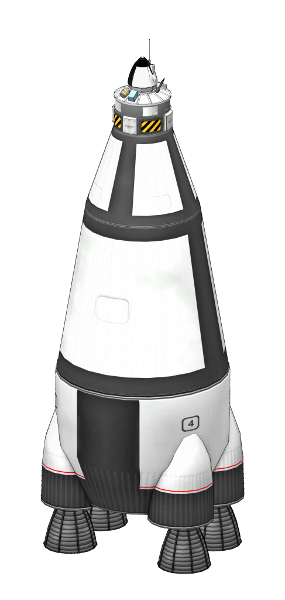
\includegraphics{pidtune_rocket_design_maxtwr8.png}
\end{figure}

Those fuel-tank adapters are from the \href{https://kerbalstuff.com/mod/148/Modular\%20Rocket\%20Systems\%20-\%20Parts\%20Pack}{Modular Rocket Systems (MRS) addon}, but stock tanks will work just fine. The design goal of this rocket is to have a TWR of 8 on the launchpad and enough fuel to make it past 30km when throttled for optimal atmospheric efficiency.
\setbox0\vbox{
\begin{minipage}{0.95\linewidth}
\textbf{Contents}

\medskip

\begin{itemize}
\item {} 
\phantomsection\label{tutorials/pidloops:id1}{\hyperref[tutorials/pidloops:proportional-feedback-loop-p-loop]{\emph{Proportional Feedback Loop (P-loop)}}}

\item {} 
\phantomsection\label{tutorials/pidloops:id2}{\hyperref[tutorials/pidloops:proportional-integral-feedback-loop-pi-loop]{\emph{Proportional-Integral Feedback Loop (PI-loop)}}}

\item {} 
\phantomsection\label{tutorials/pidloops:id3}{\hyperref[tutorials/pidloops:proportional-integral-derivative-feedback-loop-pid-loop]{\emph{Proportional-Integral-Derivative Feedback Loop (PID-loop)}}}

\item {} 
\phantomsection\label{tutorials/pidloops:id4}{\hyperref[tutorials/pidloops:final-touches]{\emph{Final Touches}}}

\item {} 
\phantomsection\label{tutorials/pidloops:id5}{\hyperref[tutorials/pidloops:tuning-a-pid-loop]{\emph{Tuning a PID-loop}}}

\item {} 
\phantomsection\label{tutorials/pidloops:id6}{\hyperref[tutorials/pidloops:final-thoughts]{\emph{Final Thoughts}}}

\end{itemize}
\end{minipage}}
\begin{center}\setlength{\fboxsep}{5pt}\shadowbox{\box0}\end{center}


\subsection{Proportional Feedback Loop (P-loop)}
\label{tutorials/pidloops:proportional-feedback-loop-p-loop}
The example code from the {\hyperref[tutorials/designpatterns:designpatterns]{\emph{\DUspan{}{Design Patterns Tutorial}}}}, with some slight modifications looks like the following:

\begin{Verbatim}[commandchars=\\\{\}]
\PYG{c+c1}{// staging, throttle, steering, go}
\PYG{n}{WHEN} \PYG{n+nl}{STAGE}\PYG{p}{:}\PYG{n}{LIQUIDFUEL} \PYG{o}{\PYGZlt{}} \PYG{l+m+mf}{0.1} \PYG{n}{THEN} \PYG{p}{\PYGZob{}}
    \PYG{n}{STAGE}\PYG{p}{.}
    \PYG{n}{PRESERVE}\PYG{p}{.}
\PYG{p}{\PYGZcb{}}
\PYG{n}{LOCK} \PYG{n}{THROTTLE} \PYG{n}{TO} \PYG{l+m+mf}{1.}
\PYG{n}{LOCK} \PYG{n}{STEERING} \PYG{n}{TO} \PYG{n}{R}\PYG{p}{(}\PYG{l+m+mi}{0}\PYG{p}{,}\PYG{l+m+mi}{0}\PYG{p}{,}\PYG{o}{\PYGZhy{}}\PYG{l+m+mi}{90}\PYG{p}{)} \PYG{o}{+} \PYG{n}{HEADING}\PYG{p}{(}\PYG{l+m+mi}{90}\PYG{p}{,}\PYG{l+m+mi}{90}\PYG{p}{)}\PYG{p}{.}
\PYG{n}{STAGE}\PYG{p}{.}
\PYG{n}{WAIT} \PYG{n}{UNTIL} \PYG{n+nl}{SHIP}\PYG{p}{:}\PYG{n}{ALTITUDE} \PYG{o}{\PYGZgt{}} \PYG{l+m+mf}{1000.}

\PYG{c+c1}{// P\PYGZhy{}loop setup}
\PYG{n}{SET} \PYG{n}{g} \PYG{n}{TO} \PYG{n+nl}{KERBIN}\PYG{p}{:}\PYG{n}{MU} \PYG{o}{/} \PYG{n+nl}{KERBIN}\PYG{p}{:}\PYG{n}{RADIUS}\PYG{o}{\PYGZca{}}\PYG{l+m+mf}{2.}
\PYG{n}{LOCK} \PYG{n}{accvec} \PYG{n}{TO} \PYG{n+nl}{SHIP}\PYG{p}{:}\PYG{n+nl}{SENSORS}\PYG{p}{:}\PYG{n}{ACC} \PYG{o}{\PYGZhy{}} \PYG{n+nl}{SHIP}\PYG{p}{:}\PYG{n+nl}{SENSORS}\PYG{p}{:}\PYG{n}{GRAV}\PYG{p}{.}
\PYG{n}{LOCK} \PYG{n}{gforce} \PYG{n}{TO} \PYG{n+nl}{accvec}\PYG{p}{:}\PYG{n}{MAG} \PYG{o}{/} \PYG{n}{g}\PYG{p}{.}
\PYG{n}{LOCK} \PYG{n}{dthrott} \PYG{n}{TO} \PYG{l+m+mf}{0.05} \PYG{o}{*} \PYG{p}{(}\PYG{l+m+mf}{1.2} \PYG{o}{\PYGZhy{}} \PYG{n}{gforce}\PYG{p}{)}\PYG{p}{.}

\PYG{n}{SET} \PYG{n}{thrott} \PYG{n}{TO} \PYG{l+m+mf}{1.}
\PYG{n}{LOCK} \PYG{n}{THROTTLE} \PYG{n}{to} \PYG{n}{thrott}\PYG{p}{.}

\PYG{n}{UNTIL} \PYG{n+nl}{SHIP}\PYG{p}{:}\PYG{n}{ALTITUDE} \PYG{o}{\PYGZgt{}} \PYG{l+m+mi}{40000} \PYG{p}{\PYGZob{}}
    \PYG{n}{SET} \PYG{n}{thrott} \PYG{n}{to} \PYG{n}{thrott} \PYG{o}{+} \PYG{n}{dthrott}\PYG{p}{.}
    \PYG{n}{WAIT} \PYG{l+m+mf}{0.1}\PYG{p}{.}
\PYG{p}{\PYGZcb{}}
\end{Verbatim}

The first several lines sets up a simple staging condition, puts the throttle to maximum, steers the rocket straight up and launches. The rocket is assumed to use only liquid fuel engines. After the rocket hits 1km, the script sets up the LOCK used in the P-loop which is updated every 0.1 seconds in the UNTIL loop. The use of LOCK variables makes this code fairly clean. When the script comes up to the first line in the UNTIL loop, i.e. ``SET thrott TO thrott + dthrott.'', the variable dthrott is evaluated which causes the LOCK on gforce to be evaluated which in-turn causes accvec to be evaluated.

The input to this feedback loop is the acceleration experienced by the ship (gforce) in terms of Kerbin's gravitational acceleration at sea level (g). The variable accvec is the total acceleration vector and is obtained by the accelerometer and gravioli detectors, both of which must be on the ship for this to work. The variable dthrott is the change in throttle that should be applied in a single iteration of the feedback loop.

In terms of a PID loop, the factor 1.2 is called the setpoint, gforce is the process variable and 0.05 is called the proportional gain. The setpoint and gain factors can be promoted to their own variables with names. Also, the code up to and including the ``WAIT UNTIL SHIP:ALTITUDE \textgreater{} 1000.'' will be implied for the next few examples of code:

\begin{Verbatim}[commandchars=\\\{\}]
\PYG{c+c1}{// P\PYGZhy{}loop}
\PYG{n}{SET} \PYG{n}{g} \PYG{n}{TO} \PYG{n+nl}{KERBIN}\PYG{p}{:}\PYG{n}{MU} \PYG{o}{/} \PYG{n+nl}{KERBIN}\PYG{p}{:}\PYG{n}{RADIUS}\PYG{o}{\PYGZca{}}\PYG{l+m+mf}{2.}
\PYG{n}{LOCK} \PYG{n}{accvec} \PYG{n}{TO} \PYG{n+nl}{SHIP}\PYG{p}{:}\PYG{n+nl}{SENSORS}\PYG{p}{:}\PYG{n}{ACC} \PYG{o}{\PYGZhy{}} \PYG{n+nl}{SHIP}\PYG{p}{:}\PYG{n+nl}{SENSORS}\PYG{p}{:}\PYG{n}{GRAV}\PYG{p}{.}
\PYG{n}{LOCK} \PYG{n}{gforce} \PYG{n}{TO} \PYG{n+nl}{accvec}\PYG{p}{:}\PYG{n}{MAG} \PYG{o}{/} \PYG{n}{g}\PYG{p}{.}

\PYG{n}{SET} \PYG{n}{gforce\PYGZus{}setpoint} \PYG{n}{TO} \PYG{l+m+mf}{1.2}\PYG{p}{.}
\PYG{n}{SET} \PYG{n}{Kp} \PYG{n}{TO} \PYG{l+m+mf}{0.05}\PYG{p}{.}
\PYG{n}{LOCK} \PYG{n}{dthrott} \PYG{n}{TO} \PYG{n}{Kp} \PYG{o}{*} \PYG{p}{(}\PYG{n}{gforce\PYGZus{}setpoint} \PYG{o}{\PYGZhy{}} \PYG{n}{gforce}\PYG{p}{)}\PYG{p}{.}

\PYG{n}{SET} \PYG{n}{thrott} \PYG{n}{TO} \PYG{l+m+mf}{1.}
\PYG{n}{LOCK} \PYG{n}{THROTTLE} \PYG{n}{to} \PYG{n}{thrott}\PYG{p}{.}

\PYG{n}{UNTIL} \PYG{n+nl}{SHIP}\PYG{p}{:}\PYG{n}{ALTITUDE} \PYG{o}{\PYGZgt{}} \PYG{l+m+mi}{40000} \PYG{p}{\PYGZob{}}
    \PYG{n}{SET} \PYG{n}{thrott} \PYG{n}{to} \PYG{n}{thrott} \PYG{o}{+} \PYG{n}{dthrott}\PYG{p}{.}
    \PYG{n}{WAIT} \PYG{l+m+mf}{0.1}\PYG{p}{.}
\PYG{p}{\PYGZcb{}}
\end{Verbatim}

This is not a big change, but it will set us up to include the integral and derivative terms in the next section.


\subsection{Proportional-Integral Feedback Loop (PI-loop)}
\label{tutorials/pidloops:proportional-integral-feedback-loop-pi-loop}
Adding the integral term requires us to keep track of time. This is done by introducing a variable (t0) to store the time of the last iteration. Now, the throttle is changed only on iterations where some time has elapsed so the WAIT time in the UNTIL can be brought to 0.001. The offset of the gforce has been set to the variable P, and the integral gain to Ki.

\begin{Verbatim}[commandchars=\\\{\}]
\PYG{c+c1}{// PI\PYGZhy{}loop}
\PYG{n}{SET} \PYG{n}{g} \PYG{n}{TO} \PYG{n+nl}{KERBIN}\PYG{p}{:}\PYG{n}{MU} \PYG{o}{/} \PYG{n+nl}{KERBIN}\PYG{p}{:}\PYG{n}{RADIUS}\PYG{o}{\PYGZca{}}\PYG{l+m+mf}{2.}
\PYG{n}{LOCK} \PYG{n}{accvec} \PYG{n}{TO} \PYG{n+nl}{SHIP}\PYG{p}{:}\PYG{n+nl}{SENSORS}\PYG{p}{:}\PYG{n}{ACC} \PYG{o}{\PYGZhy{}} \PYG{n+nl}{SHIP}\PYG{p}{:}\PYG{n+nl}{SENSORS}\PYG{p}{:}\PYG{n}{GRAV}\PYG{p}{.}
\PYG{n}{LOCK} \PYG{n}{gforce} \PYG{n}{TO} \PYG{n+nl}{accvec}\PYG{p}{:}\PYG{n}{MAG} \PYG{o}{/} \PYG{n}{g}\PYG{p}{.}

\PYG{n}{SET} \PYG{n}{gforce\PYGZus{}setpoint} \PYG{n}{TO} \PYG{l+m+mf}{1.2}\PYG{p}{.}

\PYG{n}{LOCK} \PYG{n}{P} \PYG{n}{TO} \PYG{n}{gforce\PYGZus{}setpoint} \PYG{o}{\PYGZhy{}} \PYG{n}{gforce}\PYG{p}{.}
\PYG{n}{SET} \PYG{n}{I} \PYG{n}{TO} \PYG{l+m+mf}{0.}

\PYG{n}{SET} \PYG{n}{Kp} \PYG{n}{TO} \PYG{l+m+mf}{0.01}\PYG{p}{.}
\PYG{n}{SET} \PYG{n}{Ki} \PYG{n}{TO} \PYG{l+m+mf}{0.006}\PYG{p}{.}

\PYG{n}{LOCK} \PYG{n}{dthrott} \PYG{n}{TO} \PYG{n}{Kp} \PYG{o}{*} \PYG{n}{P} \PYG{o}{+} \PYG{n}{Ki} \PYG{o}{*} \PYG{n}{I}\PYG{p}{.}

\PYG{n}{SET} \PYG{n}{thrott} \PYG{n}{TO} \PYG{l+m+mf}{1.}
\PYG{n}{LOCK} \PYG{n}{THROTTLE} \PYG{n}{to} \PYG{n}{thrott}\PYG{p}{.}

\PYG{n}{SET} \PYG{n}{t0} \PYG{n}{TO} \PYG{n+nl}{TIME}\PYG{p}{:}\PYG{n}{SECONDS}\PYG{p}{.}
\PYG{n}{UNTIL} \PYG{n+nl}{SHIP}\PYG{p}{:}\PYG{n}{ALTITUDE} \PYG{o}{\PYGZgt{}} \PYG{l+m+mi}{40000} \PYG{p}{\PYGZob{}}
    \PYG{n}{SET} \PYG{n}{dt} \PYG{n}{TO} \PYG{n+nl}{TIME}\PYG{p}{:}\PYG{n}{SECONDS} \PYG{o}{\PYGZhy{}} \PYG{n}{t0}\PYG{p}{.}
    \PYG{n}{IF} \PYG{n}{dt} \PYG{o}{\PYGZgt{}} \PYG{l+m+mi}{0} \PYG{p}{\PYGZob{}}
        \PYG{n}{SET} \PYG{n}{I} \PYG{n}{TO} \PYG{n}{I} \PYG{o}{+} \PYG{n}{P} \PYG{o}{*} \PYG{n}{dt}\PYG{p}{.}
        \PYG{n}{SET} \PYG{n}{thrott} \PYG{n}{to} \PYG{n}{thrott} \PYG{o}{+} \PYG{n}{dthrott}\PYG{p}{.}
        \PYG{n}{SET} \PYG{n}{t0} \PYG{n}{TO} \PYG{n+nl}{TIME}\PYG{p}{:}\PYG{n}{SECONDS}\PYG{p}{.}
    \PYG{p}{\PYGZcb{}}
    \PYG{n}{WAIT} \PYG{l+m+mf}{0.001}\PYG{p}{.}
\PYG{p}{\PYGZcb{}}
\end{Verbatim}

Adding the integral term has the general effect of stabilizing the feedback loop, making it less prone to oscillating due to rapid changes in the process variable (gforce, in this case). This is usually at the expense of a longer settling time.


\subsection{Proportional-Integral-Derivative Feedback Loop (PID-loop)}
\label{tutorials/pidloops:proportional-integral-derivative-feedback-loop-pid-loop}
Incorporating the derivative term (D) and derivative gain (Kd) requires an additional variable (P0) to keep track of the previous value of the proportional term (P).

\begin{Verbatim}[commandchars=\\\{\}]
\PYG{c+c1}{// PID\PYGZhy{}loop}
\PYG{n}{SET} \PYG{n}{g} \PYG{n}{TO} \PYG{n+nl}{KERBIN}\PYG{p}{:}\PYG{n}{MU} \PYG{o}{/} \PYG{n+nl}{KERBIN}\PYG{p}{:}\PYG{n}{RADIUS}\PYG{o}{\PYGZca{}}\PYG{l+m+mf}{2.}
\PYG{n}{LOCK} \PYG{n}{accvec} \PYG{n}{TO} \PYG{n+nl}{SHIP}\PYG{p}{:}\PYG{n+nl}{SENSORS}\PYG{p}{:}\PYG{n}{ACC} \PYG{o}{\PYGZhy{}} \PYG{n+nl}{SHIP}\PYG{p}{:}\PYG{n+nl}{SENSORS}\PYG{p}{:}\PYG{n}{GRAV}\PYG{p}{.}
\PYG{n}{LOCK} \PYG{n}{gforce} \PYG{n}{TO} \PYG{n+nl}{accvec}\PYG{p}{:}\PYG{n}{MAG} \PYG{o}{/} \PYG{n}{g}\PYG{p}{.}

\PYG{n}{SET} \PYG{n}{gforce\PYGZus{}setpoint} \PYG{n}{TO} \PYG{l+m+mf}{1.2}\PYG{p}{.}

\PYG{n}{LOCK} \PYG{n}{P} \PYG{n}{TO} \PYG{n}{gforce\PYGZus{}setpoint} \PYG{o}{\PYGZhy{}} \PYG{n}{gforce}\PYG{p}{.}
\PYG{n}{SET} \PYG{n}{I} \PYG{n}{TO} \PYG{l+m+mf}{0.}
\PYG{n}{SET} \PYG{n}{D} \PYG{n}{TO} \PYG{l+m+mf}{0.}
\PYG{n}{SET} \PYG{n}{P0} \PYG{n}{TO} \PYG{n}{P}\PYG{p}{.}

\PYG{n}{SET} \PYG{n}{Kp} \PYG{n}{TO} \PYG{l+m+mf}{0.01}\PYG{p}{.}
\PYG{n}{SET} \PYG{n}{Ki} \PYG{n}{TO} \PYG{l+m+mf}{0.006}\PYG{p}{.}
\PYG{n}{SET} \PYG{n}{Kd} \PYG{n}{TO} \PYG{l+m+mf}{0.006}\PYG{p}{.}

\PYG{n}{LOCK} \PYG{n}{dthrott} \PYG{n}{TO} \PYG{n}{Kp} \PYG{o}{*} \PYG{n}{P} \PYG{o}{+} \PYG{n}{Ki} \PYG{o}{*} \PYG{n}{I} \PYG{o}{+} \PYG{n}{Kd} \PYG{o}{*} \PYG{n}{D}\PYG{p}{.}

\PYG{n}{SET} \PYG{n}{thrott} \PYG{n}{TO} \PYG{l+m+mf}{1.}
\PYG{n}{LOCK} \PYG{n}{THROTTLE} \PYG{n}{to} \PYG{n}{thrott}\PYG{p}{.}

\PYG{n}{SET} \PYG{n}{t0} \PYG{n}{TO} \PYG{n+nl}{TIME}\PYG{p}{:}\PYG{n}{SECONDS}\PYG{p}{.}
\PYG{n}{UNTIL} \PYG{n+nl}{SHIP}\PYG{p}{:}\PYG{n}{ALTITUDE} \PYG{o}{\PYGZgt{}} \PYG{l+m+mi}{40000} \PYG{p}{\PYGZob{}}
    \PYG{n}{SET} \PYG{n}{dt} \PYG{n}{TO} \PYG{n+nl}{TIME}\PYG{p}{:}\PYG{n}{SECONDS} \PYG{o}{\PYGZhy{}} \PYG{n}{t0}\PYG{p}{.}
    \PYG{n}{IF} \PYG{n}{dt} \PYG{o}{\PYGZgt{}} \PYG{l+m+mi}{0} \PYG{p}{\PYGZob{}}
        \PYG{n}{SET} \PYG{n}{I} \PYG{n}{TO} \PYG{n}{I} \PYG{o}{+} \PYG{n}{P} \PYG{o}{*} \PYG{n}{dt}\PYG{p}{.}
        \PYG{n}{SET} \PYG{n}{D} \PYG{n}{TO} \PYG{p}{(}\PYG{n}{P} \PYG{o}{\PYGZhy{}} \PYG{n}{P0}\PYG{p}{)} \PYG{o}{/} \PYG{n}{dt}\PYG{p}{.}
        \PYG{n}{SET} \PYG{n}{thrott} \PYG{n}{to} \PYG{n}{thrott} \PYG{o}{+} \PYG{n}{dthrott}\PYG{p}{.}
        \PYG{n}{SET} \PYG{n}{P0} \PYG{n}{TO} \PYG{n}{P}\PYG{p}{.}
        \PYG{n}{SET} \PYG{n}{t0} \PYG{n}{TO} \PYG{n+nl}{TIME}\PYG{p}{:}\PYG{n}{SECONDS}\PYG{p}{.}
    \PYG{p}{\PYGZcb{}}
    \PYG{n}{WAIT} \PYG{l+m+mf}{0.001}\PYG{p}{.}
\PYG{p}{\PYGZcb{}}
\end{Verbatim}

When tuned properly, the derivative term will cause the PID-loop to act quickly without causing problematic oscillations. Later in this tutorial, we will cover a way to tune a PID-loop using only the proportional term called the Zieger-Nichols method.


\subsection{Final Touches}
\label{tutorials/pidloops:final-touches}
There are a few modifications that can make PID loops very robust. The following code example adds three range limits:
\begin{enumerate}
\item {} 
bounds on the Integral term which addresses possible \href{http://en.wikipedia.org/wiki/Integral\_windup}{integral windup}

\item {} 
bounds on the throttle since it must stay in the range 0 to 1

\item {} 
a \href{http://en.wikipedia.org/wiki/Deadband}{deadband} to avoid changing the throttle due to small fluctuations

\end{enumerate}

Of course, KSP is a simulator and small fluctuations are not observed in this particular loop. Indeed, the P-loop is sufficient in this example, but all these features are included here for illustration purposes and they could become useful for unstable aircraft or untested scenarios.

\begin{Verbatim}[commandchars=\\\{\}]
\PYG{c+c1}{// PID\PYGZhy{}loop}
\PYG{n}{SET} \PYG{n}{g} \PYG{n}{TO} \PYG{n+nl}{KERBIN}\PYG{p}{:}\PYG{n}{MU} \PYG{o}{/} \PYG{n+nl}{KERBIN}\PYG{p}{:}\PYG{n}{RADIUS}\PYG{o}{\PYGZca{}}\PYG{l+m+mf}{2.}
\PYG{n}{LOCK} \PYG{n}{accvec} \PYG{n}{TO} \PYG{n+nl}{SHIP}\PYG{p}{:}\PYG{n+nl}{SENSORS}\PYG{p}{:}\PYG{n}{ACC} \PYG{o}{\PYGZhy{}} \PYG{n+nl}{SHIP}\PYG{p}{:}\PYG{n+nl}{SENSORS}\PYG{p}{:}\PYG{n}{GRAV}\PYG{p}{.}
\PYG{n}{LOCK} \PYG{n}{gforce} \PYG{n}{TO} \PYG{n+nl}{accvec}\PYG{p}{:}\PYG{n}{MAG} \PYG{o}{/} \PYG{n}{g}\PYG{p}{.}

\PYG{n}{SET} \PYG{n}{gforce\PYGZus{}setpoint} \PYG{n}{TO} \PYG{l+m+mf}{1.2}\PYG{p}{.}

\PYG{n}{LOCK} \PYG{n}{P} \PYG{n}{TO} \PYG{n}{gforce\PYGZus{}setpoint} \PYG{o}{\PYGZhy{}} \PYG{n}{gforce}\PYG{p}{.}
\PYG{n}{SET} \PYG{n}{I} \PYG{n}{TO} \PYG{l+m+mf}{0.}
\PYG{n}{SET} \PYG{n}{D} \PYG{n}{TO} \PYG{l+m+mf}{0.}
\PYG{n}{SET} \PYG{n}{P0} \PYG{n}{TO} \PYG{n}{P}\PYG{p}{.}

\PYG{n}{LOCK} \PYG{n}{in\PYGZus{}deadband} \PYG{n}{TO} \PYG{n}{ABS}\PYG{p}{(}\PYG{n}{P}\PYG{p}{)} \PYG{o}{\PYGZlt{}} \PYG{l+m+mf}{0.01}\PYG{p}{.}

\PYG{n}{SET} \PYG{n}{Kp} \PYG{n}{TO} \PYG{l+m+mf}{0.01}\PYG{p}{.}
\PYG{n}{SET} \PYG{n}{Ki} \PYG{n}{TO} \PYG{l+m+mf}{0.006}\PYG{p}{.}
\PYG{n}{SET} \PYG{n}{Kd} \PYG{n}{TO} \PYG{l+m+mf}{0.006}\PYG{p}{.}

\PYG{n}{LOCK} \PYG{n}{dthrott} \PYG{n}{TO} \PYG{n}{Kp} \PYG{o}{*} \PYG{n}{P} \PYG{o}{+} \PYG{n}{Ki} \PYG{o}{*} \PYG{n}{I} \PYG{o}{+} \PYG{n}{Kd} \PYG{o}{*} \PYG{n}{D}\PYG{p}{.}

\PYG{n}{SET} \PYG{n}{thrott} \PYG{n}{TO} \PYG{l+m+mf}{1.}
\PYG{n}{LOCK} \PYG{n}{THROTTLE} \PYG{n}{to} \PYG{n}{thrott}\PYG{p}{.}

\PYG{n}{SET} \PYG{n}{t0} \PYG{n}{TO} \PYG{n+nl}{TIME}\PYG{p}{:}\PYG{n}{SECONDS}\PYG{p}{.}
\PYG{n}{UNTIL} \PYG{n+nl}{SHIP}\PYG{p}{:}\PYG{n}{ALTITUDE} \PYG{o}{\PYGZgt{}} \PYG{l+m+mi}{40000} \PYG{p}{\PYGZob{}}
    \PYG{n}{SET} \PYG{n}{dt} \PYG{n}{TO} \PYG{n+nl}{TIME}\PYG{p}{:}\PYG{n}{SECONDS} \PYG{o}{\PYGZhy{}} \PYG{n}{t0}\PYG{p}{.}
    \PYG{n}{IF} \PYG{n}{dt} \PYG{o}{\PYGZgt{}} \PYG{l+m+mi}{0} \PYG{p}{\PYGZob{}}
        \PYG{n}{IF} \PYG{n}{NOT} \PYG{n}{in\PYGZus{}deadband} \PYG{p}{\PYGZob{}}
            \PYG{n}{SET} \PYG{n}{I} \PYG{n}{TO} \PYG{n}{I} \PYG{o}{+} \PYG{n}{P} \PYG{o}{*} \PYG{n}{dt}\PYG{p}{.}
            \PYG{n}{SET} \PYG{n}{D} \PYG{n}{TO} \PYG{p}{(}\PYG{n}{P} \PYG{o}{\PYGZhy{}} \PYG{n}{P0}\PYG{p}{)} \PYG{o}{/} \PYG{n}{dt}\PYG{p}{.}

            \PYG{c+c1}{// If Ki is non\PYGZhy{}zero, then limit Ki*I to [\PYGZhy{}1,1]}
            \PYG{n}{IF} \PYG{n}{Ki} \PYG{o}{\PYGZgt{}} \PYG{l+m+mi}{0} \PYG{p}{\PYGZob{}}
                \PYG{n}{SET} \PYG{n}{I} \PYG{n}{TO} \PYG{n}{MIN}\PYG{p}{(}\PYG{l+m+mf}{1.0}\PYG{o}{/}\PYG{n}{Ki}\PYG{p}{,} \PYG{n}{MAX}\PYG{p}{(}\PYG{o}{\PYGZhy{}}\PYG{l+m+mf}{1.0}\PYG{o}{/}\PYG{n}{Ki}\PYG{p}{,} \PYG{n}{I}\PYG{p}{)}\PYG{p}{)}\PYG{p}{.}
            \PYG{p}{\PYGZcb{}}

            \PYG{c+c1}{// set throttle but keep in range [0,1]}
            \PYG{n}{SET} \PYG{n}{thrott} \PYG{n}{to} \PYG{n}{MIN}\PYG{p}{(}\PYG{l+m+mi}{1}\PYG{p}{,} \PYG{n}{MAX}\PYG{p}{(}\PYG{l+m+mi}{0}\PYG{p}{,} \PYG{n}{thrott} \PYG{o}{+} \PYG{n}{dthrott}\PYG{p}{)}\PYG{p}{)}\PYG{p}{.}

            \PYG{n}{SET} \PYG{n}{P0} \PYG{n}{TO} \PYG{n}{P}\PYG{p}{.}
            \PYG{n}{SET} \PYG{n}{t0} \PYG{n}{TO} \PYG{n+nl}{TIME}\PYG{p}{:}\PYG{n}{SECONDS}\PYG{p}{.}
        \PYG{p}{\PYGZcb{}}
    \PYG{p}{\PYGZcb{}}
    \PYG{n}{WAIT} \PYG{l+m+mf}{0.001}\PYG{p}{.}
\PYG{p}{\PYGZcb{}}
\end{Verbatim}


\subsection{Tuning a PID-loop}
\label{tutorials/pidloops:tuning-a-pid-loop}
We are going to start with the same rocket design we have been using so far and actually tune the PID-loop using the Ziegler-Nichols method. This is where we turn off the integral and derivative terms in the loop and bring the proportional gain (Kp) up from zero to the point where the loop causes a steady oscillation with a measured period (Tu). At this point, the proportional gain is called the ``ultimate gain'' (Ku) and the actual gains (Kp, Ki and Kd) are set according to this table \href{http://en.wikipedia.org/wiki/Ziegler\%E2\%80\%93Nichols\_method}{taken from wikipedia}:

\begin{tabulary}{\linewidth}{|L|L|L|L|}
\hline
\textsf{\relax 
Control Type
} & \textsf{\relax 
Kp
} & \textsf{\relax 
Ki
} & \textsf{\relax 
Kd
}\\
\hline
P
 & 
0.5 Ku
 &  & \\
\hline
PI
 & 
0.45 Ku
 & 
1.2 Kp / Tu
 & \\
\hline
PD
 & 
0.8 Ku
 &  & 
Kp Tu / 8
\\
\hline
classic PID
 & 
0.6 Ku
 & 
2 Kp / Tu
 & 
Kp Tu / 8
\\
\hline
Pessen Integral Rule
 & 
0.7 Ku
 & 
0.4 Kp / Tu
 & 
0.15 Kp Tu
\\
\hline
some overshoot
 & 
0.33 Ku
 & 
2 Kp / Tu
 & 
Kp Tu / 3
\\
\hline
no overshoot
 & 
0.2 Ku
 & 
2 Kp / Tu
 & 
Kp Tu / 3
\\
\hline\end{tabulary}


An immediate problem to overcome with this method is that it assumes a steady state can be achieved. With rockets, there is never a steady state: fuel is being consumed, altitude and therefore gravity and atmosphere is changing, staging can cause major upsets in the feedback loop. So, this tuning method will be some approximation which should come as no surprise since it will come from experimental observation. All we need is enough of a steady state that we can measure the oscillations - both the change in amplitude and the period.

The script we'll use to tune the highly overpowered rocket shown will launch the rocket straight up (using SAS) and will log data to an output file until it reaches 30km at which point the log file will be copied to the archive and the program will terminate. Also, this time the feedback loop will be based on the more realistic ``atmospheric efficiency.'' The log file will contain three columns: time since launch, offset of atmospheric efficiency from the ideal (in this case, 1.0) and the ship's maximum thrust. The maximum thrust will increase monotonically with time (this rocket has only one stage) and we'll use both as the x-axis when plotting the offset on the y-axis.

\begin{Verbatim}[commandchars=\\\{\}]
\PYG{n}{DECLARE} \PYG{n}{PARAMETER} \PYG{n}{Kp}\PYG{p}{.}

\PYG{n}{LOCK} \PYG{n}{g} \PYG{n}{TO} \PYG{n+nl}{SHIP}\PYG{p}{:}\PYG{n+nl}{BODY}\PYG{p}{:}\PYG{n}{MU} \PYG{o}{/} \PYG{p}{(}\PYG{n+nl}{SHIP}\PYG{p}{:}\PYG{n+nl}{BODY}\PYG{p}{:}\PYG{n}{RADIUS} \PYG{o}{+} \PYG{n+nl}{SHIP}\PYG{p}{:}\PYG{n}{ALTITUDE}\PYG{p}{)}\PYG{o}{\PYGZca{}}\PYG{l+m+mf}{2.}
\PYG{n}{LOCK} \PYG{n}{maxtwr} \PYG{n}{TO} \PYG{n+nl}{SHIP}\PYG{p}{:}\PYG{n}{MAXTHRUST} \PYG{o}{/} \PYG{p}{(}\PYG{n}{g} \PYG{o}{*} \PYG{n+nl}{SHIP}\PYG{p}{:}\PYG{n}{MASS}\PYG{p}{)}\PYG{p}{.}

\PYG{c+c1}{// feedback based on atmospheric efficiency}
\PYG{n}{LOCK} \PYG{n}{surfspeed} \PYG{n}{TO} \PYG{n+nl}{SHIP}\PYG{p}{:}\PYG{n+nl}{VELOCITY}\PYG{p}{:}\PYG{n+nl}{SURFACE}\PYG{p}{:}\PYG{n}{MAG}\PYG{p}{.}
\PYG{n}{LOCK} \PYG{n}{atmoeff} \PYG{n}{TO} \PYG{n}{surfspeed} \PYG{o}{/} \PYG{n+nl}{SHIP}\PYG{p}{:}\PYG{n}{TERMVELOCITY}\PYG{p}{.}
\PYG{n}{LOCK} \PYG{n}{P} \PYG{n}{TO} \PYG{l+m+mf}{1.0} \PYG{o}{\PYGZhy{}} \PYG{n}{atmoeff}\PYG{p}{.}

\PYG{n}{SET} \PYG{n}{t0} \PYG{n}{TO} \PYG{n+nl}{TIME}\PYG{p}{:}\PYG{n}{SECONDS}\PYG{p}{.}
\PYG{n}{LOCK} \PYG{n}{dthrott} \PYG{n}{TO} \PYG{n}{Kp}\PYG{o}{*}\PYG{n}{P}\PYG{p}{.}
\PYG{n}{SET} \PYG{n}{start\PYGZus{}time} \PYG{n}{TO} \PYG{n}{t0}\PYG{p}{.}

\PYG{n}{LOG} \PYG{l+s}{\PYGZdq{}}\PYG{l+s}{\PYGZsh{} Throttle PID Tuning}\PYG{l+s}{\PYGZdq{}} \PYG{n}{TO} \PYG{n}{throttle\PYGZus{}log}\PYG{p}{.}
\PYG{n}{LOG} \PYG{l+s}{\PYGZdq{}}\PYG{l+s}{\PYGZsh{} Kp: }\PYG{l+s}{\PYGZdq{}} \PYG{o}{+} \PYG{n}{Kp} \PYG{n}{TO} \PYG{n}{throttle\PYGZus{}log}\PYG{p}{.}
\PYG{n}{LOG} \PYG{l+s}{\PYGZdq{}}\PYG{l+s}{\PYGZsh{} t P maxtwr}\PYG{l+s}{\PYGZdq{}} \PYG{n}{TO} \PYG{n}{throttle\PYGZus{}log}\PYG{p}{.}

\PYG{n}{LOCK} \PYG{n}{logline} \PYG{n}{TO} \PYG{p}{(}\PYG{n+nl}{TIME}\PYG{p}{:}\PYG{n}{SECONDS} \PYG{o}{\PYGZhy{}} \PYG{n}{start\PYGZus{}time}\PYG{p}{)}
        \PYG{o}{+} \PYG{l+s}{\PYGZdq{}}\PYG{l+s}{ }\PYG{l+s}{\PYGZdq{}} \PYG{o}{+} \PYG{n}{P}
        \PYG{o}{+} \PYG{l+s}{\PYGZdq{}}\PYG{l+s}{ }\PYG{l+s}{\PYGZdq{}} \PYG{o}{+} \PYG{n}{maxtwr}\PYG{p}{.}

\PYG{n}{SET} \PYG{n}{thrott} \PYG{n}{TO} \PYG{l+m+mf}{1.}
\PYG{n}{LOCK} \PYG{n}{THROTTLE} \PYG{n}{TO} \PYG{n}{thrott}\PYG{p}{.}
\PYG{n}{SAS} \PYG{n}{ON}\PYG{p}{.}
\PYG{n}{STAGE}\PYG{p}{.}
\PYG{n}{WAIT} \PYG{l+m+mf}{3.}

\PYG{n}{UNTIL} \PYG{n+nl}{SHIP}\PYG{p}{:}\PYG{n}{ALTITUDE} \PYG{o}{\PYGZgt{}} \PYG{l+m+mi}{30000} \PYG{p}{\PYGZob{}}
    \PYG{n}{SET} \PYG{n}{dt} \PYG{n}{TO} \PYG{n+nl}{TIME}\PYG{p}{:}\PYG{n}{SECONDS} \PYG{o}{\PYGZhy{}} \PYG{n}{t0}\PYG{p}{.}
    \PYG{n}{IF} \PYG{n}{dt} \PYG{o}{\PYGZgt{}} \PYG{l+m+mi}{0} \PYG{p}{\PYGZob{}}
        \PYG{n}{SET} \PYG{n}{thrott} \PYG{n}{TO} \PYG{n}{MIN}\PYG{p}{(}\PYG{l+m+mi}{1}\PYG{p}{,}\PYG{n}{MAX}\PYG{p}{(}\PYG{l+m+mi}{0}\PYG{p}{,}\PYG{n}{thrott} \PYG{o}{+} \PYG{n}{dthrott}\PYG{p}{)}\PYG{p}{)}\PYG{p}{.}
        \PYG{n}{SET} \PYG{n}{t0} \PYG{n}{TO} \PYG{n+nl}{TIME}\PYG{p}{:}\PYG{n}{SECONDS}\PYG{p}{.}
        \PYG{n}{LOG} \PYG{n}{logline} \PYG{n}{TO} \PYG{n}{throttle\PYGZus{}log}\PYG{p}{.}
    \PYG{p}{\PYGZcb{}}
    \PYG{n}{WAIT} \PYG{l+m+mf}{0.001}\PYG{p}{.}
\PYG{p}{\PYGZcb{}}
\PYG{n}{COPY} \PYG{n}{throttle\PYGZus{}log} \PYG{n}{TO} \PYG{l+m+mf}{0.}
\end{Verbatim}

Give this script a short name, something like ``tune.txt'' so that running is simple:

\begin{Verbatim}[commandchars=\\\{\}]
\PYG{n}{copy} \PYG{n}{tune} \PYG{n}{from} \PYG{l+m+mf}{0.}
\PYG{n}{run} \PYG{n}{tune}\PYG{p}{(}\PYG{l+m+mf}{0.5}\PYG{p}{)}\PYG{p}{.}
\end{Verbatim}

After every launch completes, you'll have to go into the archive directory and rename the output logfile. Something like ``throttle\_log.txt'' --\textgreater{} ``throttle.01.log'' will help if you increment the index number each time. To analyze the data, plot the offset (P) as a function of time (t). Here, we show the results for three values of Kp: 0.002, 0.016 and 0.160, including the maximum TWR when Kp = 0.002 as the top x-axis. The maximum TWR dependence on time is different for the three values of Kp, but not by a lot.
\begin{figure}[htbp]
\centering

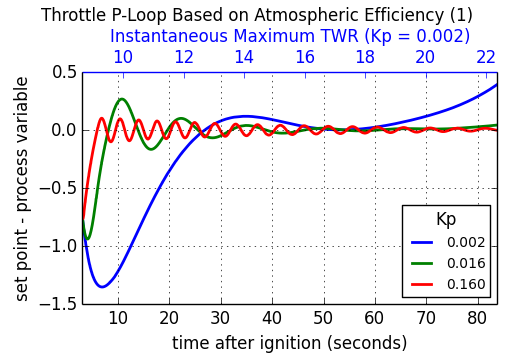
\includegraphics{pidtune1.png}
\end{figure}

The value of 0.002 is obviously too low. The settling time is well over 20 seconds and the loop can't keep up with the increase in terminal velocity at the higher altitudes reached after one minute. When Kp = 0.016, the behavior is far more well behaved, and though some oscillation exists, it's damped and slow with a period of about 10 seconds. At Kp = 0.160, the oscillations are prominent and we can start to measure the change in amplitude along with the period of the oscillations. This plot shows the data for Kp = 0.160 from 20 to 40 seconds after ignition. The peaks are found and are fit to a line.
\begin{figure}[htbp]
\centering

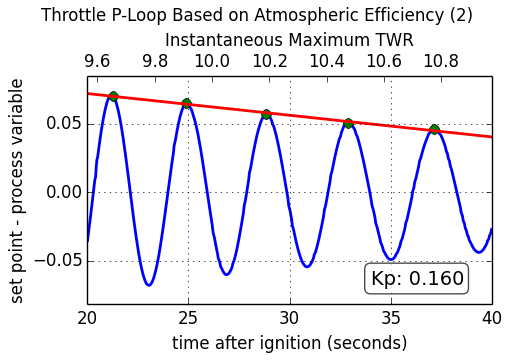
\includegraphics{pidtune2.png}
\end{figure}

This is done for each value of Kp and the slopes of the fitted lines are plotted as a function of Kp in the following plot:
\begin{figure}[htbp]
\centering

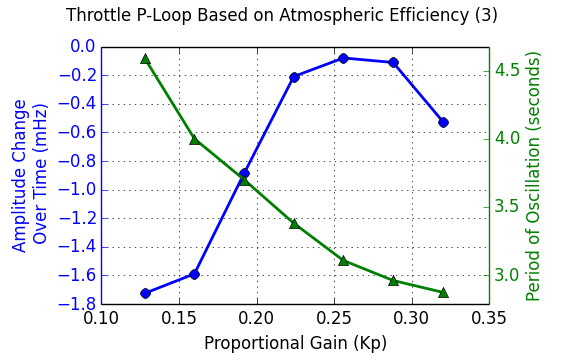
\includegraphics{pidtune3.png}
\end{figure}

The period of oscillation was averaged over the interval and plotted on top of the amplitude change over time. Notice the turn over that occurs when Kp reaches approximately 0.26. This will mark the ``ultimate gain'' and 3.1 seconds will be used as the associated period of oscillation. It is left as an exercise for the reader to implement a full PID-loop using the classic PID values (see table above): Kp = 0.156, Ki = 0.101, Kd = 0.060, producing this behavior:
\begin{figure}[htbp]
\centering

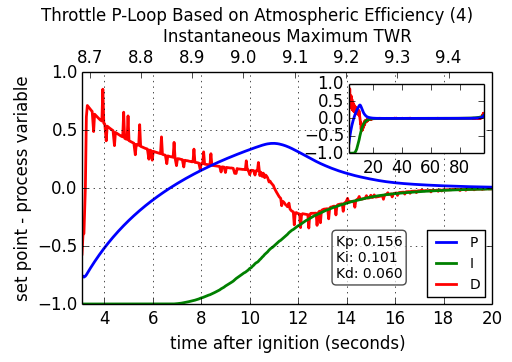
\includegraphics{pidtune4.png}
\end{figure}

As soon as the PID-loop was activated at 3 seconds after ignition, the throttle was cut. At approximately 7 seconds, the atmospheric efficiency dropped below 100\% and the integral term started to climb back to zero. At 11 seconds, the engine was reignited and the feedback loop settled after about 20 seconds. The inset plot has the same axes as the parent and shows the long-term stability of the final PID-loop.


\subsection{Final Thoughts}
\label{tutorials/pidloops:final-thoughts}
The classic PID values used above are fairly aggressive and there is some overshoot at the beginning. This can be dealt with in many ways and is discussed on the \href{http://en.wikipedia.org/wiki/PID\_controller}{wikipedia page about PID controllers}. For example, one might consider trying to implement a switch to a PD-loop when the integral term hits some limit, switching back once P crosses zero. The PID behavior should look like the following:
\begin{figure}[htbp]
\centering

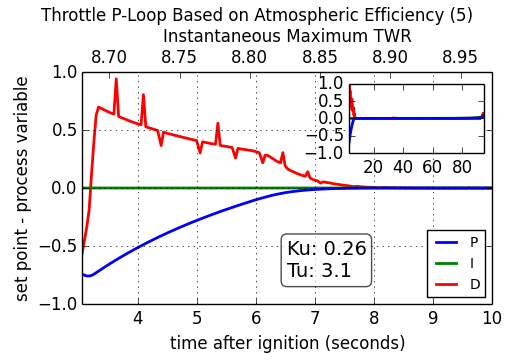
\includegraphics{pidtune5.png}
\label{tutorials/pidloops:wikipedia-page-about-pid-controllers}\end{figure}

Finally, Controlling the throttle of a rocket is perhaps the easiest thing to implement as a PID loop in KSP using kOS. The steering was largely ignored and the orientation was always up. When writing an autopilot for horizontal atmospheric flight, one will have to deal with the direction the ship is traveling using SHIP:HEADING as well as it's orientation with SHIP:FACING. Additionally, there are the SHIP:ROTATION and SHIP:TRANSLATION vectors which can tell you the rate of change of the ship's facing and heading respectively. The controls in this case are six-dimensional using SHIP:CONTROL with YAW, PITCH, ROLL, FORE, STARBOARD, TOP and MAINTHROTTLE.

The PID gain parameters are dependent on the characteristics of the ship being controlled. The size, shape, turning capability and maximum TWR should be considered when tuning a PID loop. Turning RCS on can also have an effect and you might consider changing the PID loop's gain parameters every time to switch them on or off.


\section{Advanced Tutorial}
\label{tutorials/exenode:advanced-tutorial}\label{tutorials/exenode:exenode}\label{tutorials/exenode::doc}
Let's try to automate one of the most common tasks in orbital maneuvering - execution of the maneuver node. In this tutorial I'll try to show you how to write a script for precise maneuver node execution.

So to start our script we need to get the next available {\hyperref[structures/vessels/node:maneuver-node]{\emph{\DUspan{}{maneuver node}}}}:

\begin{Verbatim}[commandchars=\\\{\}]
\PYG{n}{set} \PYG{n}{nd} \PYG{n}{to} \PYG{n}{nextnode}\PYG{p}{(}\PYG{p}{)}\PYG{p}{.}
\end{Verbatim}

Our next step is to calculate how much time our vessel needs to burn at full throttle to execute the node:

\begin{Verbatim}[commandchars=\\\{\}]
\PYG{c+c1}{//print out node\PYGZsq{}s basic parameters \PYGZhy{} ETA and deltaV}
\PYG{n}{print} \PYG{l+s}{\PYGZdq{}}\PYG{l+s}{Node in: }\PYG{l+s}{\PYGZdq{}} \PYG{o}{+} \PYG{n}{round}\PYG{p}{(}\PYG{n+nl}{nd}\PYG{p}{:}\PYG{n}{eta}\PYG{p}{)} \PYG{o}{+} \PYG{l+s}{\PYGZdq{}}\PYG{l+s}{, DeltaV: }\PYG{l+s}{\PYGZdq{}} \PYG{o}{+} \PYG{n}{round}\PYG{p}{(}\PYG{n+nl}{nd}\PYG{p}{:}\PYG{n+nl}{deltav}\PYG{p}{:}\PYG{n}{mag}\PYG{p}{)}\PYG{p}{.}

\PYG{c+c1}{//calculate ship\PYGZsq{}s max acceleration}
\PYG{n}{set} \PYG{n}{max\PYGZus{}acc} \PYG{n}{to} \PYG{n+nl}{ship}\PYG{p}{:}\PYG{n}{maxthrust}\PYG{o}{/}\PYG{n+nl}{ship}\PYG{p}{:}\PYG{n}{mass}\PYG{p}{.}

\PYG{c+c1}{//now we just need to divide deltav:mag by our ship\PYGZsq{}s max acceleration}
\PYG{n}{set} \PYG{n}{burn\PYGZus{}duration} \PYG{n}{to} \PYG{n+nl}{nd}\PYG{p}{:}\PYG{n+nl}{deltav}\PYG{p}{:}\PYG{n}{mag}\PYG{o}{/}\PYG{n}{max\PYGZus{}acc}\PYG{p}{.}
\PYG{n}{print} \PYG{l+s}{\PYGZdq{}}\PYG{l+s}{Estimated burn duration: }\PYG{l+s}{\PYGZdq{}} \PYG{o}{+} \PYG{n}{round}\PYG{p}{(}\PYG{n}{burn\PYGZus{}duration}\PYG{p}{)} \PYG{o}{+} \PYG{l+s}{\PYGZdq{}}\PYG{l+s}{s}\PYG{l+s}{\PYGZdq{}}\PYG{p}{.}
\end{Verbatim}

So now we have our node's deltav vector, ETA to the node and we calculated our burn duration. All that is left for us to do is wait until we are close to node's ETA less half of our burn duration. But we want to write a universal script, and some of our current and/or future ships can be quite slow to turn, so let's give us some time, 60 seconds, to prepare for the maneuver burn:

\begin{Verbatim}[commandchars=\\\{\}]
\PYG{n}{wait} \PYG{n}{until} \PYG{n+nl}{node}\PYG{p}{:}\PYG{n}{eta} \PYG{o}{\PYGZlt{}}\PYG{o}{=} \PYG{p}{(}\PYG{n}{burn\PYGZus{}duration}\PYG{o}{/}\PYG{l+m+mi}{2} \PYG{o}{+} \PYG{l+m+mi}{60}\PYG{p}{)}\PYG{p}{.}
\end{Verbatim}

This wait can be tedious and you'll most likely end up warping some time, but we'll leave kOS automation of warping for a given period of time to our readers.

The wait has finished, and now we need to start turning our ship in the direction of the burn:

\begin{Verbatim}[commandchars=\\\{\}]
\PYG{n}{set} \PYG{n}{np} \PYG{n}{to} \PYG{n}{lookdirup}\PYG{p}{(}\PYG{n+nl}{nd}\PYG{p}{:}\PYG{n}{deltav}\PYG{p}{,} \PYG{n+nl}{ship}\PYG{p}{:}\PYG{n+nl}{facing}\PYG{p}{:}\PYG{n}{topvector}\PYG{p}{)}\PYG{p}{.} \PYG{c+c1}{//points to node, keeping roll the same.}
\PYG{n}{lock} \PYG{n}{steering} \PYG{n}{to} \PYG{n}{np}\PYG{p}{.}

\PYG{c+c1}{//now we need to wait until the burn vector and ship\PYGZsq{}s facing are aligned}
\PYG{n}{wait} \PYG{n}{until} \PYG{n}{abs}\PYG{p}{(}\PYG{n+nl}{np}\PYG{p}{:}\PYG{n}{pitch} \PYG{o}{\PYGZhy{}} \PYG{n+nl}{facing}\PYG{p}{:}\PYG{n}{pitch}\PYG{p}{)} \PYG{o}{\PYGZlt{}} \PYG{l+m+mf}{0.15} \PYG{n}{and} \PYG{n}{abs}\PYG{p}{(}\PYG{n+nl}{np}\PYG{p}{:}\PYG{n}{yaw} \PYG{o}{\PYGZhy{}} \PYG{n+nl}{facing}\PYG{p}{:}\PYG{n}{yaw}\PYG{p}{)} \PYG{o}{\PYGZlt{}} \PYG{l+m+mf}{0.15}\PYG{p}{.}

\PYG{c+c1}{//the ship is facing the right direction, let\PYGZsq{}s wait for our burn time}
\PYG{n}{wait} \PYG{n}{until} \PYG{n+nl}{node}\PYG{p}{:}\PYG{n}{eta} \PYG{o}{\PYGZlt{}}\PYG{o}{=} \PYG{p}{(}\PYG{n}{burn\PYGZus{}duration}\PYG{o}{/}\PYG{l+m+mi}{2}\PYG{p}{)}
\end{Verbatim}

Now we are ready to burn. It is usually done in the \emph{until} loop, checking main parameters of the burn every iteration until the burn is complete:

\begin{Verbatim}[commandchars=\\\{\}]
\PYG{c+c1}{//we only need to lock throttle once to a certain variable in the beginning of the loop, and adjust only the variable itself inside it}
\PYG{n}{set} \PYG{n}{tset} \PYG{n}{to} \PYG{l+m+mf}{0.}
\PYG{n}{lock} \PYG{n}{throttle} \PYG{n}{to} \PYG{n}{tset}\PYG{p}{.}

\PYG{n}{set} \PYG{n}{done} \PYG{n}{to} \PYG{n}{False}\PYG{p}{.}
\PYG{c+c1}{//initial deltav}
\PYG{n}{set} \PYG{n}{dv0} \PYG{n}{to} \PYG{n+nl}{nd}\PYG{p}{:}\PYG{n}{deltav}\PYG{p}{.}
\PYG{n}{until} \PYG{n}{done}
\PYG{p}{\PYGZob{}}
    \PYG{c+c1}{//recalculate current max\PYGZus{}acceleration, as it changes while we burn through fuel}
    \PYG{n}{set} \PYG{n}{max\PYGZus{}acc} \PYG{n}{to} \PYG{n+nl}{ship}\PYG{p}{:}\PYG{n}{maxthrust}\PYG{o}{/}\PYG{n+nl}{ship}\PYG{p}{:}\PYG{n}{mass}\PYG{p}{.}

    \PYG{c+c1}{//throttle is 100\PYGZpc{} until there is less than 1 second of time left to burn}
    \PYG{c+c1}{//when there is less than 1 second \PYGZhy{} decrease the throttle linearly}
    \PYG{n}{set} \PYG{n}{tset} \PYG{n}{to} \PYG{n}{min}\PYG{p}{(}\PYG{n+nl}{nd}\PYG{p}{:}\PYG{n+nl}{deltav}\PYG{p}{:}\PYG{n}{mag}\PYG{o}{/}\PYG{n}{max\PYGZus{}acc}\PYG{p}{,} \PYG{l+m+mi}{1}\PYG{p}{)}\PYG{p}{.}

    \PYG{c+c1}{//here\PYGZsq{}s the tricky part, we need to cut the throttle as soon as our nd:deltav and initial deltav start facing opposite directions}
    \PYG{c+c1}{//this check is done via checking the dot product of those 2 vectors}
    \PYG{k}{if} \PYG{n}{vdot}\PYG{p}{(}\PYG{n}{dv0}\PYG{p}{,} \PYG{n+nl}{nd}\PYG{p}{:}\PYG{n}{deltav}\PYG{p}{)} \PYG{o}{\PYGZlt{}} \PYG{l+m+mi}{0}
    \PYG{p}{\PYGZob{}}
        \PYG{n}{print} \PYG{l+s}{\PYGZdq{}}\PYG{l+s}{End burn, remain dv }\PYG{l+s}{\PYGZdq{}} \PYG{o}{+} \PYG{n}{round}\PYG{p}{(}\PYG{n+nl}{nd}\PYG{p}{:}\PYG{n+nl}{deltav}\PYG{p}{:}\PYG{n}{mag}\PYG{p}{,}\PYG{l+m+mi}{1}\PYG{p}{)} \PYG{o}{+} \PYG{l+s}{\PYGZdq{}}\PYG{l+s}{m/s, vdot: }\PYG{l+s}{\PYGZdq{}} \PYG{o}{+} \PYG{n}{round}\PYG{p}{(}\PYG{n}{vdot}\PYG{p}{(}\PYG{n}{dv0}\PYG{p}{,} \PYG{n+nl}{nd}\PYG{p}{:}\PYG{n}{deltav}\PYG{p}{)}\PYG{p}{,}\PYG{l+m+mi}{1}\PYG{p}{)}\PYG{p}{.}
        \PYG{n}{lock} \PYG{n}{throttle} \PYG{n}{to} \PYG{l+m+mf}{0.}
        \PYG{k}{break}\PYG{p}{.}
    \PYG{p}{\PYGZcb{}}

    \PYG{c+c1}{//we have very little left to burn, less then 0.1m/s}
    \PYG{k}{if} \PYG{n+nl}{nd}\PYG{p}{:}\PYG{n+nl}{deltav}\PYG{p}{:}\PYG{n}{mag} \PYG{o}{\PYGZlt{}} \PYG{l+m+mf}{0.1}
    \PYG{p}{\PYGZob{}}
        \PYG{n}{print} \PYG{l+s}{\PYGZdq{}}\PYG{l+s}{Finalizing burn, remain dv }\PYG{l+s}{\PYGZdq{}} \PYG{o}{+} \PYG{n}{round}\PYG{p}{(}\PYG{n+nl}{nd}\PYG{p}{:}\PYG{n+nl}{deltav}\PYG{p}{:}\PYG{n}{mag}\PYG{p}{,}\PYG{l+m+mi}{1}\PYG{p}{)} \PYG{o}{+} \PYG{l+s}{\PYGZdq{}}\PYG{l+s}{m/s, vdot: }\PYG{l+s}{\PYGZdq{}} \PYG{o}{+} \PYG{n}{round}\PYG{p}{(}\PYG{n}{vdot}\PYG{p}{(}\PYG{n}{dv0}\PYG{p}{,} \PYG{n+nl}{nd}\PYG{p}{:}\PYG{n}{deltav}\PYG{p}{)}\PYG{p}{,}\PYG{l+m+mi}{1}\PYG{p}{)}\PYG{p}{.}
        \PYG{c+c1}{//we burn slowly until our node vector starts to drift significantly from initial vector}
        \PYG{c+c1}{//this usually means we are on point}
        \PYG{n}{wait} \PYG{n}{until} \PYG{n}{vdot}\PYG{p}{(}\PYG{n}{dv0}\PYG{p}{,} \PYG{n+nl}{nd}\PYG{p}{:}\PYG{n}{deltav}\PYG{p}{)} \PYG{o}{\PYGZlt{}} \PYG{l+m+mf}{0.5}\PYG{p}{.}

        \PYG{n}{lock} \PYG{n}{throttle} \PYG{n}{to} \PYG{l+m+mf}{0.}
        \PYG{n}{print} \PYG{l+s}{\PYGZdq{}}\PYG{l+s}{End burn, remain dv }\PYG{l+s}{\PYGZdq{}} \PYG{o}{+} \PYG{n}{round}\PYG{p}{(}\PYG{n+nl}{nd}\PYG{p}{:}\PYG{n+nl}{deltav}\PYG{p}{:}\PYG{n}{mag}\PYG{p}{,}\PYG{l+m+mi}{1}\PYG{p}{)} \PYG{o}{+} \PYG{l+s}{\PYGZdq{}}\PYG{l+s}{m/s, vdot: }\PYG{l+s}{\PYGZdq{}} \PYG{o}{+} \PYG{n}{round}\PYG{p}{(}\PYG{n}{vdot}\PYG{p}{(}\PYG{n}{dv0}\PYG{p}{,} \PYG{n+nl}{nd}\PYG{p}{:}\PYG{n}{deltav}\PYG{p}{)}\PYG{p}{,}\PYG{l+m+mi}{1}\PYG{p}{)}\PYG{p}{.}
        \PYG{n}{set} \PYG{n}{done} \PYG{n}{to} \PYG{n}{True}\PYG{p}{.}
    \PYG{p}{\PYGZcb{}}
\PYG{p}{\PYGZcb{}}
\PYG{n}{unlock} \PYG{n}{steering}\PYG{p}{.}
\PYG{n}{unlock} \PYG{n}{throttle}\PYG{p}{.}
\PYG{n}{wait} \PYG{l+m+mf}{1.}

\PYG{c+c1}{//we no longer need the maneuver node}
\PYG{n}{remove} \PYG{n}{nd}\PYG{p}{.}

\PYG{c+c1}{//set throttle to 0 just in case.}
\PYG{n}{SET} \PYG{n+nl}{SHIP}\PYG{p}{:}\PYG{n+nl}{CONTROL}\PYG{p}{:}\PYG{n}{PILOTMAINTHROTTLE} \PYG{n}{TO} \PYG{l+m+mf}{0.}
\end{Verbatim}

That is all, this short script can execute any maneuver node with 0.1 m/s dv precision or even better.


\section{Introductory}
\label{tutorials:introductory}\begin{description}
\item[{{\hyperref[tutorials/quickstart::doc]{\emph{\emph{Quick Start Tutorial}}}}}] \leavevmode
Walks you through the beginnings of making a beginner's ship launcher script.

\end{description}


\section{Intermediate}
\label{tutorials:intermediate}\begin{description}
\item[{{\hyperref[tutorials/designpatterns::doc]{\emph{\emph{Design Patterns Tutorial}}}}}] \leavevmode
Discusses some general aspects of kOS flow control and optimizations.

\item[{{\hyperref[tutorials/pidloops::doc]{\emph{\emph{PID Loop Tutorial}}}}}] \leavevmode
Starts with a basic proportional feedback loop and develops, in stages, a complete PID-loop to control the throttle of a simple rocket design.

\item[{{\hyperref[tutorials/exenode::doc]{\emph{\emph{Execute Node script}}}}}] \leavevmode
ZiwKerman describes a generic ``execute manuever node'' script to be a one-size-fits-all solution to many situations in KSP.  If you can make a manuever node for something, exenode will execute it.

\end{description}


\chapter{Community Examples Library}
\label{library:community-examples-library}\label{library::doc}\label{library:library}
Starting with version 0.17.0 of kOS, we have decided to support
a separate repository of examples and libraries that ``live'' entirely
in kerboscript code only.  This is a useful place to find helpful
code written by other users of kOS, some of whom may be members of
the main kOS development team, and some of whom might ber users in the
community.

The separate repository is found here:

\href{https://github.com/KSP-KOS/KSLib}{https://github.com/KSP-KOS/KSLib}

Some examples of useful things you can find there are:
\begin{itemize}
\item {} 
A generic all-purpose \textbf{PID controller} function:
\begin{itemize}
\item {} 
library script: \href{https://github.com/KSP-KOS/KSLib/blob/master/library/lib\_pid.ks}{https://github.com/KSP-KOS/KSLib/blob/master/library/lib\_pid.ks}

\item {} 
documentation: \href{https://github.com/KSP-KOS/KSLib/blob/master/doc/lib\_pid.md}{https://github.com/KSP-KOS/KSLib/blob/master/doc/lib\_pid.md}

\item {} 
example \href{https://github.com/KSP-KOS/KSLib/blob/master/examples/example\_lib\_pid.ks}{https://github.com/KSP-KOS/KSLib/blob/master/examples/example\_lib\_pid.ks}

\end{itemize}

\item {} 
A library for getting \textbf{navball orientation} information:
\begin{itemize}
\item {} 
library script \href{https://github.com/KSP-KOS/KSLib/blob/master/library/lib\_navball.ks}{https://github.com/KSP-KOS/KSLib/blob/master/library/lib\_navball.ks}

\item {} 
documentation \href{https://github.com/KSP-KOS/KSLib/blob/master/doc/lib\_navball.md}{https://github.com/KSP-KOS/KSLib/blob/master/doc/lib\_navball.md}

\item {} 
example \href{https://github.com/KSP-KOS/KSLib/blob/master/examples/example\_lib\_navball.ks}{https://github.com/KSP-KOS/KSLib/blob/master/examples/example\_lib\_navball.ks}

\end{itemize}

\item {} 
An example of how to use the {\hyperref[commands/flight/systems:sasmode]{\emph{\DUspan{}{sasmode}}}} feature:
\begin{itemize}
\item {} 
example \href{https://github.com/KSP-KOS/KSLib/blob/master/examples/example\_testsasmode.ks}{https://github.com/KSP-KOS/KSLib/blob/master/examples/example\_testsasmode.ks}

\end{itemize}

\end{itemize}


\chapter{General Topics}
\label{general:general-topics}\label{general::doc}\label{general:general}
These topics discuss the interfacing between \textbf{kOS} and \textbf{Kerbal Space Program}.


\section{Catalog of Bound Variable Names}
\label{bindings:bindings}\label{bindings:catalog-of-bound-variable-names}\label{bindings::doc}
This is the list of special reserved keyword variable names that kOS
will interpret
to mean something special. If they are used as normal variable names by
your kOS script
program they may not work. Understanding them and their meaning is
crucial to creating
effective kOS scripts.


\subsection{NAMED VESSELS AND BODIES}
\label{bindings:named-vessels-and-bodies}
SHIP:

\begin{DUlineblock}{0em}
\item[] \textbf{Variable name}: SHIP
\item[] \textbf{Gettable}: yes
\item[] \textbf{Settable}: no
\item[] \textbf{Type}: Vessel
\item[] \textbf{Description}: Whichever vessel happens to be the one containing the CPU part that is running this Kerboscript code at the moment. This is the CPU Vessel.
\end{DUlineblock}

TARGET:

\begin{DUlineblock}{0em}
\item[] \textbf{Variable Name}: TARGET
\item[] \textbf{Gettable}: yes
\item[] \textbf{Settable}: yes
\item[] \textbf{Type}: Vessel or Body
\item[] \textbf{Description}: Whichever Orbitable object happens to be the one selected as the current KSP target. If set to a string, it will assume the string is the name of a vessel being targetted and set it to a vessel by that name. For best results set it to Body(``some name'') or Vessel(``some name'') explicitly.
\end{DUlineblock}


\subsection{Alias shortcuts for SHIP fields}
\label{bindings:alias-shortcuts-for-ship-fields}
The following are all alias shortcuts for accessing the fields of the
SHIP vessel.
To see their definition, please consult the
Vessel
page, as they are all just instances of the standard vessel suffixes.

\begin{longtable}{|l|l|}
\hline
\textsf{\relax 
Variable
} & \textsf{\relax 
Same as
}\\
\hline\endfirsthead

\multicolumn{2}{c}%
{{\textsf{\tablename\ \thetable{} -- continued from previous page}}} \\
\hline
\textsf{\relax 
Variable
} & \textsf{\relax 
Same as
}\\
\hline\endhead

\hline \multicolumn{2}{|r|}{{\textsf{Continued on next page}}} \\ \hline
\endfoot

\endlastfoot


HEADING
 & 
Same as SHIP:HEADING
\\
\hline
PROGRADE
 & 
Same as SHIP:PROGRADE
\\
\hline
RETROGRADE
 & 
Same as SHIP:RETROGRADE
\\
\hline
FACING
 & 
Same as SHIP:FACING
\\
\hline
MAXTHRUST
 & 
Same as SHIP:MAXTHRUST
\\
\hline
VELOCITY
 & 
Same as SHIP:VELOCITY
\\
\hline
GEOPOSITION
 & 
Same as SHIP:GEOPOSITION
\\
\hline
LATITUDE
 & 
Same as SHIP:LATITUDE
\\
\hline
LONGITUDE
 & 
Same as SHIP:LONGITUDE
\\
\hline
UP
 & 
Same as SHIP:UP
\\
\hline
NORTH
 & 
Same as SHIP:NORTH
\\
\hline
BODY
 & 
Same as SHIP:BODY
\\
\hline
ANGULARMOMENTUM
 & 
Same as SHIP:ANGULARMOMENTUM
\\
\hline
ANGULARVEL
 & 
Same as SHIP:ANGULARVEL
\\
\hline
ANGULARVELOCITY
 & 
Same as SHIP:ANGULARVEL
\\
\hline
COMMRANGE
 & 
Same as SHIP:COMMRANGE
\\
\hline
MASS
 & 
Same as SHIP:MASS
\\
\hline
VERTICALSPEED
 & 
Same as SHIP:VERTICALSPEED
\\
\hline
GROUNDSPEED
 & 
Same as SHIP:GROUNDSPEED
\\
\hline
SURFACESPEED
 & 
This has been obsoleted as of kOS 0.18.0.  Replace it with GROUNDSPEED.
\\
\hline
AIRSPEED
 & 
Same as SHIP:AIRSPEED
\\
\hline
VESSELNAME
 & 
Same as SHIP:VESSELNAME
\\
\hline
ALTITUDE
 & 
Same as SHIP:ALTITUDE
\\
\hline
APOAPSIS
 & 
Same as SHIP:APOAPSIS
\\
\hline
PERIAPSIS
 & 
Same as SHIP:PERIAPSIS
\\
\hline
SENSORS
 & 
Same as SHIP:SENSORS
\\
\hline
SRFPROGRADE
 & 
Same as SHIP:SRFPROGRADE
\\
\hline
SRFREROGRADE
 & 
Same as SHIP:SRFREROGRADE
\\
\hline
OBT
 & 
Same as SHIP:OBT
\\
\hline
STATUS
 & 
Same as SHIP:STATUS
\\
\hline
SHIPNAME
 & 
Same as SHIP:NAME
\\
\hline\end{longtable}



\subsection{Constants (pi, e, etc)}
\label{bindings:constants-pi-e-etc}
Get-only.

The variable \code{constant} provides a way to access a few
{\hyperref[math/basic:constants]{\emph{\DUspan{}{basic math and physics constants}}}}, such as Pi, Euler's
number, and so on.

Example:

\begin{Verbatim}[commandchars=\\\{\}]
\PYG{n}{print} \PYG{l+s}{\PYGZdq{}}\PYG{l+s}{Kerbin\PYGZsq{}s circumference: }\PYG{l+s}{\PYGZdq{}} \PYG{o}{+} \PYG{p}{(}\PYG{l+m+mi}{2}\PYG{o}{*}\PYG{n+nl}{constant}\PYG{p}{:}\PYG{n}{pi}\PYG{o}{*}\PYG{n+nl}{Kerbin}\PYG{p}{:}\PYG{n}{radius}\PYG{p}{)} \PYG{o}{+} \PYG{l+s}{\PYGZdq{}}\PYG{l+s}{meters.}\PYG{l+s}{\PYGZdq{}}\PYG{p}{.}
\end{Verbatim}

The full list is here: {\hyperref[math/basic:constants]{\emph{\DUspan{}{constants page}}}}.


\subsection{Terminal}
\label{bindings:terminal}
Get-only. \code{terminal} returns a {\hyperref[structures/misc/terminal:structure:TERMINAL]{\emph{\code{terminal}}}} structure describing
the attributes of the current terminal screen associated with the
CPU this script is running on.


\subsection{Core}
\label{bindings:core}
Get-only. \code{core} returns a {\hyperref[structures/core:structure:CORE]{\emph{\code{core}}}} structure referring to the CPU you
are running on.


\subsection{Stage}
\label{bindings:stage}
Get-only. \code{stage} returns a {\hyperref[structures/vessels/stage:structure:STAGE]{\emph{\code{stage}}}} structure used to count resources
in the current stage.  Not to be confused with the COMMAND stage
which triggers the next stage.


\subsection{NextNode}
\label{bindings:nextnode}
Get-only. \code{nextnode} returns the next planned manuever \code{node} in the SHIP's flight plan.  Bombs out if no such node exists.


\subsection{Resource Types}
\label{bindings:resource-types}
Any time there is a resource on the ship it can be queried. The
resources are the values that appear when you click on the upper-right
corner of the screen in the KSP window. 
\includegraphics{resources.png}

\begin{Verbatim}[commandchars=\\\{\}]
\PYG{n}{LIQUIDFUEL}
\PYG{n}{OXIDIZER}
\PYG{n}{ELECTRICCHARGE}
\PYG{n}{MONOPROPELLANT}
\PYG{n}{INTAKEAIR}
\PYG{n}{SOLIDFUEL}
\end{Verbatim}

All of the above resources can be queried using either the prefix SHIP
or STAGE, depending on whether you are trying to query how much is left
in the current stage or the entire ship:

How much liquid fuel is left in the entire ship:

\begin{Verbatim}[commandchars=\\\{\}]
\PYG{n}{PRINT} \PYG{l+s}{\PYGZdq{}}\PYG{l+s}{There is }\PYG{l+s}{\PYGZdq{}} \PYG{o}{+} \PYG{n+nl}{SHIP}\PYG{p}{:}\PYG{n}{LIQUIDFUEL} \PYG{o}{+} \PYG{l+s}{\PYGZdq{}}\PYG{l+s}{ liquid fuel on the ship.}\PYG{l+s}{\PYGZdq{}}\PYG{p}{.}
\end{Verbatim}

How much liquid fuel is left in just the current stage:

\begin{Verbatim}[commandchars=\\\{\}]
\PYG{n}{PRINT} \PYG{l+s}{\PYGZdq{}}\PYG{l+s}{There is }\PYG{l+s}{\PYGZdq{}} \PYG{o}{+} \PYG{n+nl}{STAGE}\PYG{p}{:}\PYG{n}{LIQUIDFUEL} \PYG{o}{+} \PYG{l+s}{\PYGZdq{}}\PYG{l+s}{ liquid fuel in this stage.}\PYG{l+s}{\PYGZdq{}}\PYG{p}{.}
\end{Verbatim}

How much liquid fuel is left in the target vessel:

\begin{Verbatim}[commandchars=\\\{\}]
\PYG{n}{PRINT} \PYG{l+s}{\PYGZdq{}}\PYG{l+s}{There is }\PYG{l+s}{\PYGZdq{}} \PYG{o}{+} \PYG{n+nl}{TARGET}\PYG{p}{:}\PYG{n}{LIQUIDFUEL} \PYG{o}{+} \PYG{l+s}{\PYGZdq{}}\PYG{l+s}{ liquid fuel in the target ship.}\PYG{l+s}{\PYGZdq{}}\PYG{p}{.}
\end{Verbatim}

Any other resources that you have added using other mods should be
query-able this way, provided that you spell
the term exactly as it appears in the resources window.

You can also get a list of all resources, either in SHIP: or STAGE: with the :RESOURCES suffix.


\subsection{ALT ALIAS}
\label{bindings:alt-alias}
The special variable ALT gives you
access to a few altitude predictions:

ALT:APOAPSIS

ALT:PERIAPSIS

ALT:RADAR

Further details are found on the ALT page .


\subsection{ETA ALIAS}
\label{bindings:eta-alias}
The special variable ETA gives you
access to a few time predictions:

ETA:APOAPSIS

ETA:PERIAPSIS

ETA:TRANSITION

Further details are found on the ETA page .


\subsection{ENCOUNTER}
\label{bindings:encounter}
The orbit patch describing the next encounter with a body the current
vessel will enter. If there is no such encounter coming, it will return
the special string ``None''.  If there is an encounter coming, it will
return an object {\hyperref[structures/orbits/orbit:orbit]{\emph{\DUspan{}{of type Orbit}}}}.  (i.e. to obtain the name
of the planet the encounter is with, you can do:
\code{print ENCOUNTER:BODY:NAME.}, for example.).


\subsection{BOOLEAN TOGGLE FIELDS:}
\label{bindings:boolean-toggle-fields}
These are variables that behave like boolean flags. They can be True or
False, and can be set or toggled
using the ``ON'' and ``OFF'' and ``TOGGLE'' commands.
Many of these are for action group flags.
\textbf{NOTE ABOUT ACTION GROUP FLAGS:} If the boolean flag is for an action
group, be aware that each time the
user presses the action group keypress, it \emph{toggles} the action group,
so you might need to check for both
the change in state from false to true AND the change in state from true
to false to see if the key was hit.

\begin{tabulary}{\linewidth}{|L|L|L|L|}
\hline
\textsf{\relax 
Variable Name
} & \textsf{\relax 
Can Read
} & \textsf{\relax 
Can Set
} & \textsf{\relax 
Description
}\\
\hline
SAS
 & 
yes
 & 
yes
 & 
(Same as ``SAS'' indicator on the navball.)
\\
\hline
RCS
 & 
yes
 & 
yes
 & 
(Same as ``RCS'' indicator on the navball.)
\\
\hline
GEAR
 & 
yes
 & 
yes
 & 
Is the GEAR enabled right now? (Note, KSP does some strange things with this flag, like needing to hit it twice the first time).
\\
\hline
LEGS
 & 
yes
 & 
yes
 & 
Are the landing LEGS extended? (as opposed to GEAR which is for the wheels of a plane.)
\\
\hline
CHUTES
 & 
yes
 & 
yes
 & 
Are the parachutes extended? (Treats all parachutes as one single unit. Does not activate them individually.)
\\
\hline
LIGHTS
 & 
yes
 & 
yes
 & 
Are the lights on? (like the ``U'' key in manual flight.)
\\
\hline
PANELS
 & 
yes
 & 
yes
 & 
Are the solar panels extended? (Treats all solar panels as one single unit. Does not activate them individually.)
\\
\hline
BRAKES
 & 
yes
 & 
yes
 & 
Are the brakes on?
\\
\hline
ABORT
 & 
yes
 & 
yes
 & 
Abort Action Group.
\\
\hline
AG1
 & 
yes
 & 
yes
 & 
Action Group 1.
\\
\hline
AG2
 & 
yes
 & 
yes
 & 
Action Group 2.
\\
\hline
AG3
 & 
yes
 & 
yes
 & 
Action Group 3.
\\
\hline
AG4
 & 
yes
 & 
yes
 & 
Action Group 4.
\\
\hline
AG5
 & 
yes
 & 
yes
 & 
Action Group 5.
\\
\hline
AG6
 & 
yes
 & 
yes
 & 
Action Group 6.
\\
\hline
AG7
 & 
yes
 & 
yes
 & 
Action Group 7.
\\
\hline
AG8
 & 
yes
 & 
yes
 & 
Action Group 8.
\\
\hline
AG9
 & 
yes
 & 
yes
 & 
Action Group 9.
\\
\hline
AG10
 & 
yes
 & 
yes
 & 
Action Group 10.
\\
\hline
AGn
 & 
yes
 & 
yes
 & 
If you have the Action Groups Extended mod installed, you can access its groups the same way, i.e. AG11, AG12, AG13, etc.
\\
\hline\end{tabulary}



\subsection{Flight Control}
\label{bindings:flight-control}
There are bound variables used in controlling the flight of a ship, which
can be found at the following links:

If you want to let kOS do a lot of the work of aligning to a desired
heading for you, use Cooked Control.

If you want your script to manipulate the controls directly (as in ``set
yaw axis halfway left for a few seconds (using the `A' key)'', then
use Raw Control.

If you want to be able to READ what the player is attempting to do
while your script is running, and perhaps respond to it, then use
Reading the Pilot's Control settings (i.e reading what the manual input is attempting)
(By default your script will override manual piloting attempts, but
you can read what the pilot's controls are set at and make your
autopilot take them under advisement - sort of like how a
fly-by-wire plane works.)


\subsubsection{Controls that must be used with LOCK}
\label{bindings:controls-that-must-be-used-with-lock}
\begin{Verbatim}[commandchars=\\\{\}]
\PYG{n}{THROTTLE}            \PYG{c+c1}{// Lock to a decimal value between 0 and 1.}
\PYG{n}{STEERING}            \PYG{c+c1}{// Lock to a direction, either a Vector or a Direction.}
\PYG{n}{WHEELTHROTTLE}       \PYG{c+c1}{// Separate throttle for wheels}
\PYG{n}{WHEELSTEERING}       \PYG{c+c1}{// Separate steering system for wheels}
\end{Verbatim}


\subsection{Time}
\label{bindings:time}
Time is the simulated amount of time that passed since the beginning of the game's universe epoch. (A brand new campaign that just started begins at TIME zero.)

TIME is a useful system variable for calculating the passage of time
between taking
physical measurements (i.e. to calculate how fast a phenomenon is
changing in a loop).
It returns the KSP \emph{simulated} time, rather than the actual realtime
sitting in the
chair playing the game. If everything is running smoothly on a fast
computer, one
second of simulated time will match one second of real time, but if
anything is
causing the game to stutter or lag a bit, then the simulated time will
be a bit
slower than the real time. For any script program trying to calculate
physical
properties of the KSP universe, the time that matters is the simulated
time, which
is what TIME returns.

It's important to be aware of the frozen update
nature of the kOS
computer when reading TIME.


\subsection{System Variables}
\label{bindings:system-variables}
This section is about variables that describe the things that are slightly
outside the simulated universe of the game and are more about
the game's user interface or the kOS mod itself.  They represent things
that slightly ``break the fourth wall'' and let your script access
something entirely outside the in-character experience.

\begin{Verbatim}[commandchars=\\\{\}]
\PYG{n}{PRINT} \PYG{n}{VERSION}\PYG{p}{.}            \PYG{c+c1}{// Returns operating system version number. e.g. 0.8.6}
\PYG{n}{PRINT} \PYG{n+nl}{VERSION}\PYG{p}{:}\PYG{n}{MAJOR}\PYG{p}{.}      \PYG{c+c1}{// Returns major version number. e.g. 0}
\PYG{n}{PRINT} \PYG{n+nl}{VERSION}\PYG{p}{:}\PYG{n}{MINOR}\PYG{p}{.}      \PYG{c+c1}{// Returns minor version number. e.g. 8}
\PYG{n}{PRINT} \PYG{n+nl}{VERSION}\PYG{p}{:}\PYG{n}{BUILD}\PYG{p}{.}      \PYG{c+c1}{// Returns build version number. e.g. 6}
\PYG{n}{PRINT} \PYG{n}{SESSIONTIME}\PYG{p}{.}        \PYG{c+c1}{// Returns amount of time, in seconds, from vessel load.}
\end{Verbatim}

NOTE the following important difference:

SESSIONTIME is the time since the last time this vessel was loaded from
on-rails into full physics.

TIME is the time since the entire saved game campaign started, in the
kerbal universe's time. i.e. TIME = 0 means a brand new campaign was
just started.


\subsubsection{Config}
\label{bindings:config}
CONFIG is a special variable name that refers to the configuration
settings for the kOS mod, and can be used to set or get various
options.

CONFIG has its own page for further
details.


\subsubsection{WARP and WARPMODE}
\label{bindings:warp-and-warpmode}
Time warp can be controlled with the variables
WARP and WARPMODE.  See {\hyperref[commands/flight/warp:warp]{\emph{\DUspan{}{WARP}}}}


\subsubsection{MAPVIEW}
\label{bindings:mapview}
A boolean that is both gettable and settable.

If you query MAPVIEW, it's true if on the map screen, and false if on the flight view screen.  If you SET MAPVIEW, you can cause the game to switch between mapview and flight view or visa versa.


\subsubsection{LOADDISTANCE}
\label{bindings:loaddistance}
LOADDISTANCE sets the distance from the active vessel at
which vessels get removed from the full physics engine and put
on-rails, or visa versa.  Note that as of KSP 1.0 the stock game
supports multiple different load distance settings for different
situations such that the value changes depending on where you are.
But kOS does not support this at the moment so in kOS if you set
the LOADDISTANCE, you are setting it to the same value
universally for all situations.


\subsection{SOLARPRIMEVECTOR}
\label{bindings:solarprimevector}\label{bindings:id1}
Gives the Prime Meridian {\hyperref[math/vector:structure:VECTOR]{\emph{\code{Vector}}}} for the Solar System itself, in
current Ship-Raw XYZ coordinates.

Both the {\hyperref[structures/orbits/orbit:attribute:ORBIT:LONGITUDEOFASCENDINGNODE]{\emph{\code{Orbit:LONGITUDEOFASCENDINGNODE}}}} orbit suffix and the
{\hyperref[structures/celestial_bodies/body:attribute:BODY:ROTATIONANGLE]{\emph{\code{Body:ROTATIONANGLE}}}} body suffix are expressed in terms of
degree offsets from this \emph{Prime Meridian Reference Vector}.


\subsubsection{What is the Solar Prime Reference Vector?}
\label{bindings:what-is-the-solar-prime-reference-vector}
The solar prime vector is an arbitrary vector in space used to measure
some orbital parameters that are supposed to remain fixed to space
regardless of how the planets underneath the orbit rotate, or where the
Sun is.  In a sense it can be thought of as the celestial ``prime
meridian'' of the entire solar system, rather than the ``prime meridian'' of
any one particular rotating planet or moon.

In a hypothetical Earthling's solar system our Kerbal scientists have
hypothesized may exist in a galaxy far away, Earthbound astronomers use
a reference they called the
\href{https://en.wikipedia.org/wiki/First\_Point\_of\_Aries}{First Point of Aries},
for this purpose.

For Kerbals, it refers to a more arbitrary line in space, pointing at a fixed
point in the firmament, also known as the ``skybox''.


\subsection{Addons}
\label{bindings:addons}
Get-only.  \code{addons} is a special variable used to access various extensions
to kOS that are designed to support the features introduced by some other mods.  More info can be found on the {\hyperref[addons:addons]{\emph{\DUspan{}{addons}}}} page.


\subsection{Colors}
\label{bindings:colors}
There are several bound variables associated with {\hyperref[structures/misc/colors:colors]{\emph{\DUspan{}{hardcoded colors}}}} such as WHITE, BLACK, RED, etc.  See the linked page for the full list.


\section{CPU Vessel (SHIP)}
\label{general/cpu_vessel:cpu-vessel}\label{general/cpu_vessel::doc}\label{general/cpu_vessel:cpu-vessel-ship}
\begin{notice}{note}{Note:}
When kOS documentation refers to the ``CPU vessel'', it has the following definition:
\begin{itemize}
\item {} 
The ``CPU Vessel'' is whichever vessel happens to currently contain the CPU in which the executing code is running.

\end{itemize}
\end{notice}

It's important to distinguish this from ``active vessel'', which is a KSP term referring to whichever vessel the camera is centered on, and therefore the vessel that will receive the keyboard controls for \code{W} \code{A} \code{S} \code{D} and so on.

The two terms can differ when you are in a situation where there are two vessels near each other, both of them within full physics range (i.e. 2.5 km), such as would happen during a docking operation. In such a situation it is possible for kOS programs to be running on one, both, or neither of the two vessels. The vessel on which a program is executing is not necessarily the vessel the KSP game is currently considering the ``active'' one.

\begin{notice}{note}{Note:}
The built-in variable called \code{SHIP} is always set to the current CPU vessel. Whenever you see the documentation refer to CPU vessel, you can think of that as being ``the \code{SHIP} variable''.
\end{notice}

For all places where a kOS program needs to do something with \emph{this vessel}, for the sake of centering {\hyperref[math/ref_frame:ship-raw]{\emph{\DUspan{}{SHIP-RAW}}}} coordinates, for the sake of deciding which ship is having maneuver nodes added to it and for the sake of deciding which vessel is being controlled by the autopilot. The vessel it is referring to is itself the \textbf{CPU vessel} and not necessarily what KSP thinks of as the ``active vessel''.


\section{The kOS CPU hardware}
\label{general/cpu_hardware:the-kos-cpu-hardware}\label{general/cpu_hardware::doc}\label{general/cpu_hardware:cpu-hardware}
While it's possible to write some software without knowing anything
about the underlying computer hardware, and there are good design
principles that state one should never make assumptions about the
computer hardware when writing software, there are still some basic
things about how computers work in general that a good programmer
needs to be aware of to write good code. Along those lines, the KSP
player writing a Kerboscript program needs to know a few basic things
about how the simulated kOS CPU operates in order to be able to write
more advanced scripts. This page contains that type of information.
\setbox0\vbox{
\begin{minipage}{0.95\linewidth}
\begin{itemize}
\item {} 
\phantomsection\label{general/cpu_hardware:id1}{\hyperref[general/cpu_hardware:update-ticks-and-physics-ticks]{\emph{Update Ticks and Physics Ticks}}}

\item {} 
\phantomsection\label{general/cpu_hardware:id2}{\hyperref[general/cpu_hardware:triggers]{\emph{Triggers}}}
\begin{itemize}
\item {} 
\phantomsection\label{general/cpu_hardware:id3}{\hyperref[general/cpu_hardware:do-not-loop-a-long-time-in-a-trigger-body]{\emph{Do Not Loop a Long Time in a Trigger Body!}}}

\item {} 
\phantomsection\label{general/cpu_hardware:id4}{\hyperref[general/cpu_hardware:but-i-want-a-loop]{\emph{But I Want a Loop!!}}}

\item {} 
\phantomsection\label{general/cpu_hardware:id5}{\hyperref[general/cpu_hardware:wait]{\emph{Wait!!!}}}

\end{itemize}

\item {} 
\phantomsection\label{general/cpu_hardware:id6}{\hyperref[general/cpu_hardware:the-frozen-universe]{\emph{The Frozen Universe}}}

\end{itemize}
\end{minipage}}
\begin{center}\setlength{\fboxsep}{5pt}\shadowbox{\box0}\end{center}


\subsection{Update Ticks and Physics Ticks}
\label{general/cpu_hardware:update-ticks-and-physics-ticks}\label{general/cpu_hardware:physics-tick}
\begin{notice}{note}{Note:}
\DUspan{versionmodified}{New in version 0.17: }Previous versions of kOS used to execute program code during the
Update phase, rather than the more correct Physics Update phase.
\end{notice}

Kerbal Space Program simulates the universe by running the universe in
small incremental time intervals that for the purpose of this
document, we will call ``\textbf{physics ticks}''. The exact length of time
for a physics tick varies as the program runs. One physics tick might
take 0.09 seconds while the next one might take 0.085 seconds. (The
default setting for the rate of physics ticks is 25 ticks per second,
just to give a ballpark figure, but you \textbf{must not} write any scripts
that depend on this assumption because it's a setting the user can
change, and it can also vary a bit during play depending on system
load. The setting is a target goal for the game to try to achieve, not
a guarantee. If it's a fast computer with a speedy animation frame
rate, it will try to run physics ticks less often than it runs
animation frame updates, to try to make the physics tick rate match
this setting. On the other hand, If it's a slow computer, it will try
to sacrifice animation frame rate to archive this number (meaning
physics get calculated faster than you can see the effects.)

When calculating physics formulas, you need to actually measure
elapsed time in the TIME:SECONDS variable in your scripts.

The entire simulated universe is utterly frozen during the duration of
a physics tick. For example, if one physics tick occurs at timestamp
10.51 seconds, and the next physics tick occurs 0.08 seconds later at
timestamp 10.59 seconds, then during the entire intervening time, at
timestamp 10.52 seconds, 10.53 seconds, and so on, nothing moves. The
clock is frozen at 10.51 seconds, and the fuel isn't being consumed,
and the vessel is at the same position. On the next physics tick at
10.59 seconds, then all the numbers are updated.  The full details of
the physics ticks system are more complex than that, but that quick
description is enough to describe what you need to know about how
kOS's CPU works.

There is another kind of time tick called an \textbf{Update tick}. It is
similar to, but different from, a \textbf{physics tick}. \emph{Update ticks}
often occur a bit more often than \emph{physics ticks}. Update ticks are
exactly the same thing as your game's Frame Rate. Each time your game
renders another animation frame, it performs another Update tick. On a
good gaming computer with fast speed and a good graphics card, It is
typical to have about 2 or even 3 \emph{Update ticks} happen within the
time it takes to have one \emph{physics tick} happen. On a slower computer,
it is also possible to go the other way and have \emph{Update ticks}
happening \emph{less} frequently than \emph{physics tics}. Basically, look at
your frame rate. Is it higher than 25 fps? If so, then your \emph{update
ticks} happen faster than your \emph{physics ticks}, otherwise its the
other way around.

\begin{notice}{note}{Note:}
As of version 0.17.0, The kOS CPU runs every \emph{physics tick}.
\end{notice}

On each physics tick, each kOS CPU that's within physics range (i.e. 2.5 km), wakes up and performs the following steps, in this order:
\begin{enumerate}
\item {} 
Run the conditional checks of all TRIGGERS (see below)

\item {} 
For any TRIGGERS who's conditional checks are true, execute the entire body of the trigger.

\item {} 
If there's a pending WAIT statement, check if it's done. If so wake up.

\item {} 
If awake, then execute the next {\hyperref[structures/misc/config:attribute:CONFIG:IPU]{\emph{\code{Config:IPU}}}} number of instructions of the main program.

\end{enumerate}

Note that the number of instructions being executed (CONFIG:IPU) are NOT lines of code or kerboscript statements, but rather the smaller instruction opcodes that they are compiled into behind the scenes. A single kerboscript statement might become anywhere from one to ten or so instructions when compiled.


\subsection{Triggers}
\label{general/cpu_hardware:triggers}
There are multiple things within kerboscript that run ``in the background'' always updating, while the main script continues on. The way these work is a bit like a real computer's multithreading, but not \emph{quite}. Collectively all of these things are called ``triggers''.

Triggers are all of the following:
\begin{itemize}
\item {} 
LOCKS which are attached to flight controls (THROTTLE, STEERING,
etc), but not other LOCKS.

\item {} 
ON condition \{ some commands \}.

\item {} 
WHEN condition THEN \{ some commands \}.

\end{itemize}

\begin{notice}{note}{Note:}
The {\hyperref[language/flow:wait]{\emph{\DUspan{}{WAIT}}}} command only causes mainline code
to be suspended.  Trigger code such as WHEN, ON, LOCK STEERING,
and LOCK THROTTLE, will continue executing while your program
is sitting still on the WAIT command.
\end{notice}

The way these work is that once per \textbf{physics tick}, all the LOCK expressions which directly affect flight control are re-executed, and then each conditional trigger's condition is checked, and if true, then the entire body of the trigger is executed all the way to the bottom *before any more instructions of the main body are executed*. This means that execution of a trigger never gets interleaved with the main code. Once a trigger happens, the entire trigger occurs all in one go before the rest of the main body continues.


\subsubsection{Do Not Loop a Long Time in a Trigger Body!}
\label{general/cpu_hardware:do-not-loop-a-long-time-in-a-trigger-body}
Because the entire body of a trigger will execute all the way to the bottom on \emph{within a single} \textbf{physics tick}, \emph{before} any other code continues, it is vital that you not write code in a trigger body that takes a long time to execute. The body of a trigger must be kept quick. An infinite loop in a trigger body could literally freeze all of KSP, because the kOS mod will never finish executing its update.

\emph{As of kOS version 0.14 and higher, this condition is now being checked for} and the script will be \textbf{terminated with a runtime error} if the triggers like WHEN/THEN and ON take more than {\hyperref[structures/misc/config:attribute:CONFIG:IPU]{\emph{\code{Config:IPU}}}} instructions to execute. The sum total of all the code within your WHEN/THEN and ON code blocks MUST be designed to complete within one physicd tick.

\textbf{This may seem harsh}. Ideally, kOS would only generate a runtime error if it thought your script was stuck in an \textbf{infinite loop}, and allow it to exceed the {\hyperref[structures/misc/config:attribute:CONFIG:IPU]{\emph{\code{Config:IPU}}}} number of instructions if it was going to finish and just needed a little longer to to finish its work. But, because of a well known problem in computer science called \href{http://en.wikipedia.org/wiki/Halting\_problem}{the halting problem}, it's literally impossible for kOS, or any other software for that matter, to detect the difference between another program's infinite loop versus another program's loop that will end soon. kOS only knows how long your triggers have taken so far, not how long they're going to take before they're done, or even if they'll be done.

If you suspect that your trigger body would have ended if it was allowed to run a little longer, try setting your {\hyperref[structures/misc/config:attribute:CONFIG:IPU]{\emph{\code{Config:IPU}}}} setting a bit higher and see if that makes the error go away.

If it does not make the error go away, then you will need to redesign your script to not depend on running a long-lasting amount of code inside triggers.


\subsubsection{But I Want a Loop!!}
\label{general/cpu_hardware:but-i-want-a-loop}
If you want a trigger body that is meant to loop, the only acceptable way to do it is to design it to execute just once, but then use the PRESERVE keyword to keep the trigger around for the next physics update. Thus your trigger becomes a sort of ``loop'' that executes one iteration per \textbf{physics tick}.

It is also important to consider the way triggers execute for performance reasons too. Every time you write an expression for a trigger, you are creating a bit of code that gets executed fully to the end before your main body will continue, once each \textbf{physics tick}. A complex expression in a trigger condition, which in turn calls other complex LOCK expressions, which call other complex LOCK expressions, and so on, may cause kOS to bog itself down during each physics tick. (And as of version 0.14, it may cause kOS to stop your program and issue a runtime error if it's taking too long.)

Because of how WAIT works, you cannot put a WAIT statement inside a trigger. If you try, it will have no effect. This is because WAIT requires the ability of the program to go to sleep and then in a later physics tick, continue from where it left off. Because triggers run to the bottom entirely within one physics tick, they can't do that.


\subsubsection{Wait!!!}
\label{general/cpu_hardware:wait}
Any WAIT statement causes the kerboscript program to immediately stop executing the main program where it is, even if far fewer than {\hyperref[structures/misc/config:attribute:CONFIG:IPU]{\emph{\code{Config:IPU}}}} instructions have been executed in this \textbf{physics tick}. It will not continue the execution until at least the next \textbf{physics tick}, when it will check to see if the WAIT condition is satisfied and it's time to wake up and continue.

Therefore ANY WAIT of any kind will guarantee that your program will allow at least one \textbf{physics tick} to have happened before continuing. If you attempt to:

\begin{Verbatim}[commandchars=\\\{\}]
\PYG{n}{WAIT} \PYG{l+m+mf}{0.001}\PYG{p}{.}
\end{Verbatim}

But the duration of the next physics tick is actually 0.09 seconds, then you will actually end up waiting at least 0.09 seconds. It is impossible to wait a unit of time smaller than one physics tick. Using a very small unit of time in a WAIT statement is an effective way to force the CPU to allow a physics tick to occur before continuing to the next line of code. Similarly, if you just say:

\begin{Verbatim}[commandchars=\\\{\}]
\PYG{n}{WAIT} \PYG{n}{UNTIL} \PYG{n}{TRUE}\PYG{p}{.}
\end{Verbatim}

Then even though the condition is immediately true, it will still wait one physics tick to discover this fact and continue.

\begin{notice}{note}{Note:}
The {\hyperref[language/flow:wait]{\emph{\DUspan{}{WAIT}}}} command only causes mainline code
to be suspended.  Trigger code such as WHEN, ON, LOCK STEERING,
and LOCK THROTTLE, will continue executing while your program
is sitting still on the WAIT command.
\end{notice}


\subsection{The Frozen Universe}
\label{general/cpu_hardware:the-frozen-universe}
Each \textbf{physics} \emph{tick}, the kOS mod wakes up and runs through all the currently loaded CPU parts that are in ``physics range'' (i.e. 2.5 km), and executes a batch of instructions from your script code that's on them. It is important to note that during the running of this batch of instructions, because no \textbf{physics ticks} are happening during it, none of the values that you might query from the KSP system will change. The clock time returned from the TIME variable will keep the same value throughout. The amount of fuel left will remain fixed throughout. The position and velocity of the vessel will remaining fixed throughout. It's not until the next physics tick occurs that those values will change to new numbers. It's typical that several lines of your kerboscript code will run during a single physics tick.

Effectively, as far as the \emph{simulated} universe can tell, it's as if your script runs several instructions in literally zero amount of time, and then pauses for a fraction of a second, and then runs more instructions in literally zero amount of time, then pauses for a fraction of a second, and so on, rather than running the program in a smoothed out continuous way.

This is a vital difference between how a kOS CPU behaves versus how a real world computer behaves. In a real world computer, you would know for certain that time will pass, even if it's just a few picoseconds, between the execution of one statement and the next.


\section{kOS Control Panel}
\label{general/applauncher_panel:applauncher}\label{general/applauncher_panel::doc}\label{general/applauncher_panel:kos-control-panel}
As of kOS v0.15, kOS now makes use of Kerbal Space Program's built-in
Application Launcher toolbar, to open a config/status panel for kOS.

This panel behaves like the other display panels the launcher creates,
and operates mutually exclusively with them. (For example you can't
make the kOS App Control Panel appear at the same time as the stock
Resource display panel. Opening one toggles the other one off,
and visa versa.)

Here is an annotated image of the control panel and what it does:
\begin{figure}[htbp]
\centering

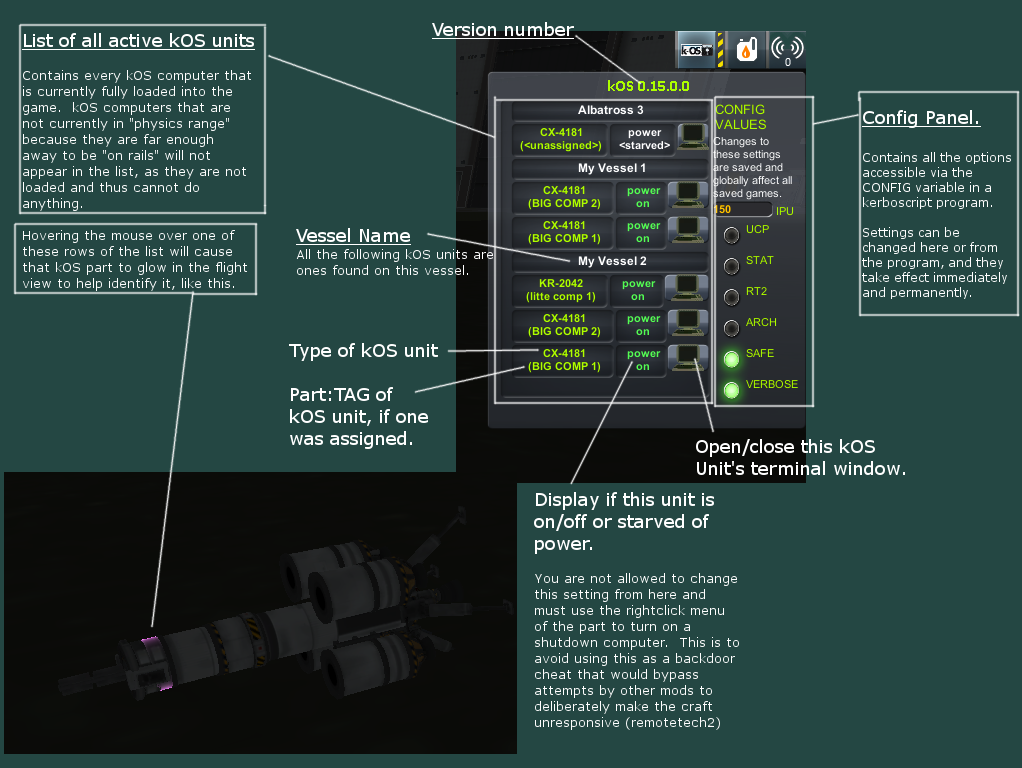
\includegraphics[width=0.800\linewidth]{applauncher_panel.png}
\end{figure}


\section{The kOS Telnet Server}
\label{general/telnet:the-kos-telnet-server}\label{general/telnet::doc}\label{general/telnet:telnet}
kOS now supports the ability to enable a \href{http://www.telnet.org/htm/faq.htm}{telnet server}
inside Kerbal Space Program.

Telnet is an old network protocol designed in the early days of the Internet, long
before World Wide Web.  Its purpose was (is) to allow you to get access to the
remote command line interfaces of distant server computers, acting as if the
keyboard and computer screen in front of you was a terminal hooked up to a distant
computer.  kOS uses this protocol to let you
\textbf{access the kOS terminal from a program outside of Kerbal Space Program}.

There are freely available programs you can use as the telnet client to
behave like terminal windows outside of the KSP window.  A list of them appears below
in the section called {\hyperref[general/telnet:telnet-clients]{\emph{Telnet clients}}}.

There are some \emph{security implications} of enabling the kOS telnet server, and the
first time you turn it on you will see some warning messages to this effect.
If you want to read further about these concerns before deciding to turn it
on, see the section called ``{\hyperref[general/telnet:security]{\emph{Security}}}'' at the bottom of this page.
\setbox0\vbox{
\begin{minipage}{0.95\linewidth}
\begin{itemize}
\item {} 
\phantomsection\label{general/telnet:id4}{\hyperref[general/telnet:telnet-clients]{\emph{Telnet clients}}}

\item {} 
\phantomsection\label{general/telnet:id5}{\hyperref[general/telnet:using-it]{\emph{Using it}}}

\item {} 
\phantomsection\label{general/telnet:id6}{\hyperref[general/telnet:special-keys]{\emph{Special Keys}}}

\item {} 
\phantomsection\label{general/telnet:id7}{\hyperref[general/telnet:howto-putty-client]{\emph{HOWTO: Putty client}}}

\item {} 
\phantomsection\label{general/telnet:id8}{\hyperref[general/telnet:howto-command-line-client]{\emph{HOWTO: Command-line client}}}

\item {} 
\phantomsection\label{general/telnet:id9}{\hyperref[general/telnet:howto-other-client]{\emph{HOWTO: Other client}}}

\item {} 
\phantomsection\label{general/telnet:id10}{\hyperref[general/telnet:security]{\emph{Security}}}

\item {} 
\phantomsection\label{general/telnet:id11}{\hyperref[general/telnet:homemade-telnet-clients]{\emph{Homemade telnet clients}}}

\end{itemize}
\end{minipage}}
\begin{center}\setlength{\fboxsep}{5pt}\shadowbox{\box0}\end{center}
\begin{figure}[htbp]
\centering

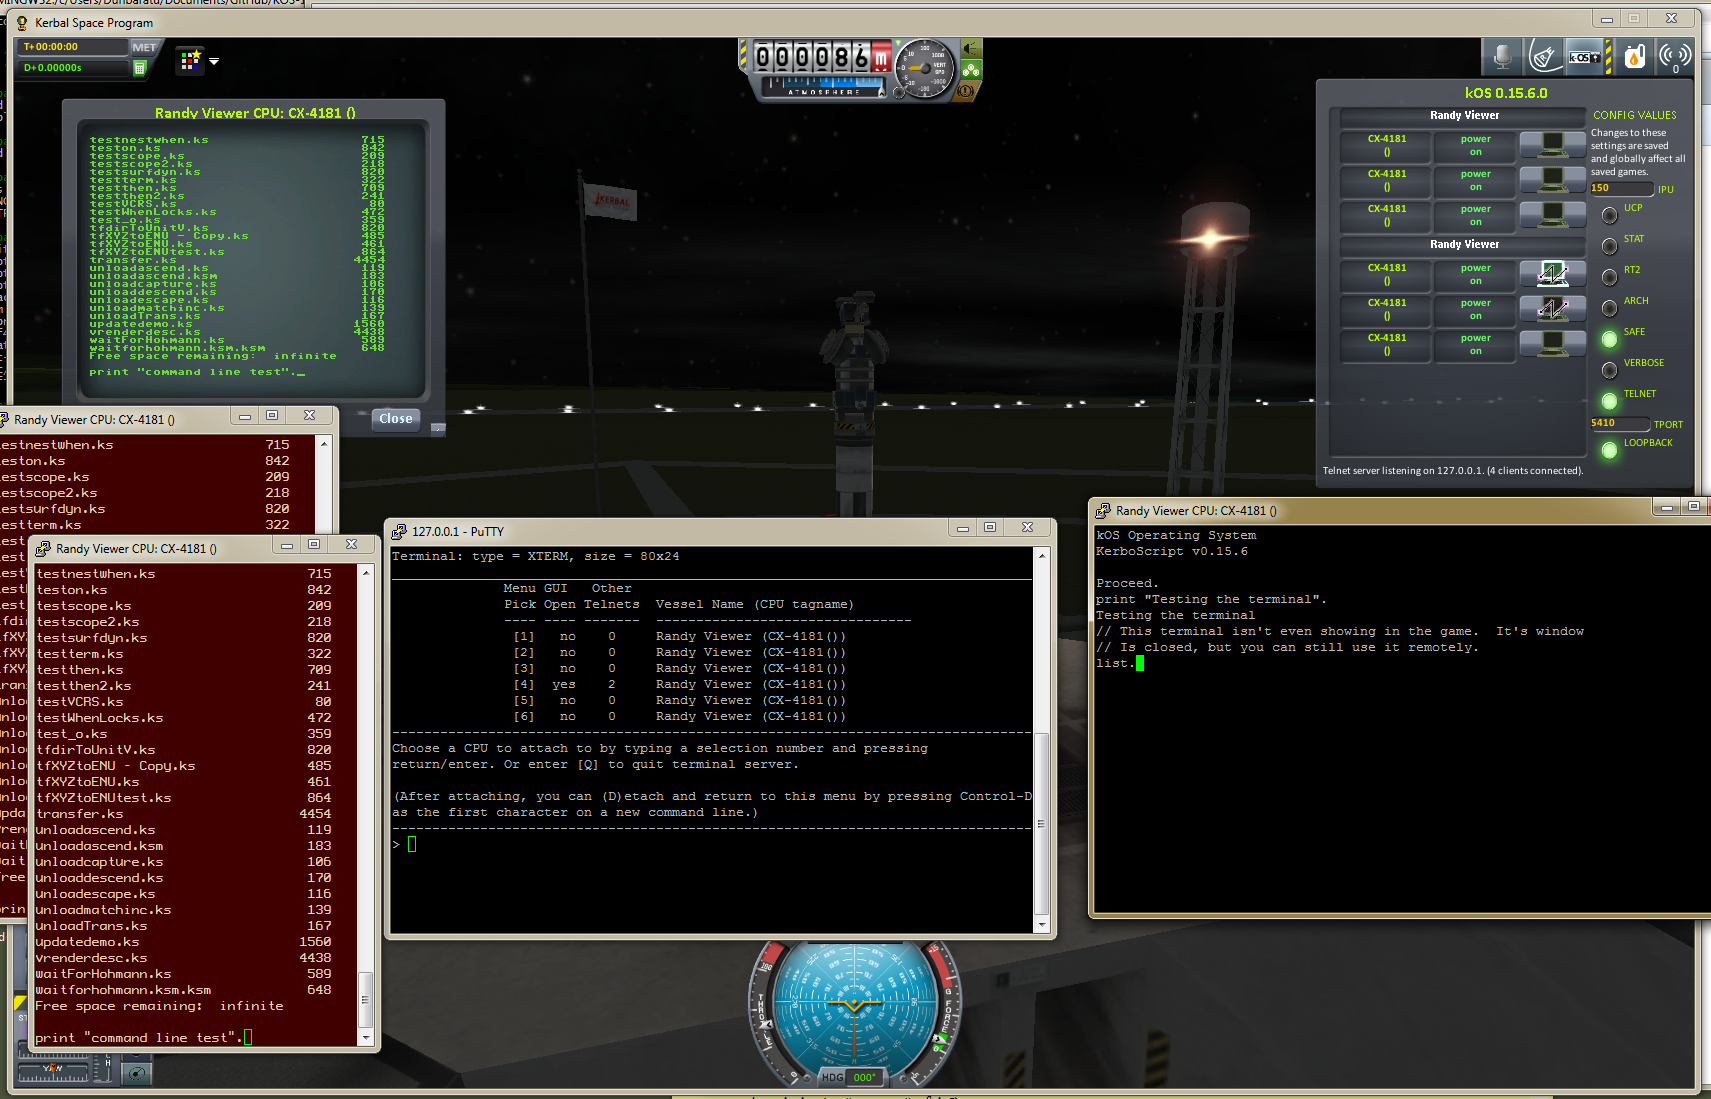
\includegraphics[width=0.950\linewidth]{telnet.png}
\end{figure}


\subsection{Telnet clients}
\label{general/telnet:telnet-clients}
The telnet server for kOS requires the use of a
\href{http://www.telnet.org/htm/applications.htm}{telnet client program}. We
recommend the following programs, although you can use others:
\begin{description}
\item[{For Windows}] \leavevmode
We recommend \href{http://www.putty.org/}{Putty}, the free terminal emulator
for Windows, although any good terminal emulator should do the job,
provided it is capable of operating in an ``XTERM - compatible'' mode.

\item[{For Mac}] \leavevmode
You shouldn't have to install anything.  There should be a telnet client
already installed, which you can access by opening up your command terminal,
and then running it as a command-line tool.  To see how to use it, read
below in the section titled ``{\hyperref[general/telnet:howto-command-line-client]{\emph{HOWTO: Command-line client}}}''.  The built-in
Terminal.app for OSX understands the XTERM command sequences that kOS uses
and in fact identifies itself as a type of XTERM when used with a telnet
client.

\item[{For Linux}] \leavevmode
You shouldn't have to install anything.  There should be a telnet client
already installed, and an xterm program already installed in most any Linux
distribution.  Open an xterm window, and in that window type the telnet
command, as described by the section titled ``{\hyperref[general/telnet:howto-command-line-client]{\emph{HOWTO: Command-line client}}}``

\end{description}


\subsection{Using it}
\label{general/telnet:using-it}\begin{enumerate}
\item {} 
Turn on the telnet server by going into the app control panel and clicking
on the green circle next to the word ``Telnet''.  Alternatively, you can
issue the command:

\begin{Verbatim}[commandchars=\\\{\}]
\PYG{n}{SET} \PYG{n+nl}{CONFIG}\PYG{p}{:}\PYG{n}{TELNET} \PYG{n}{TO} \PYG{n}{TRUE}\PYG{p}{.}
\end{Verbatim}

from any terminal window in kOS.

\item {} 
The very first time you do this, you will get a warning message, as per
\href{http://forum.kerbalspaceprogram.com/threads/87843-Forum-Rules-Add-on-Posting-Rules-August-21st-2014}{SQUAD's rule number 5 about mods that run network services}.
After accepting and clicking ``yes'', the server will be running on loopback
127.0.0.1 (if you want to make it run on the non-loopback address, you will
get a secondary warning message about that too.

\item {} 
Launch your telnet client (there is a list of telnet clients that are known
to work listed below.

\item {} 
When you first log in to the server you should see the ``Welcome menu'', which is a
screen looking like this:

\begin{Verbatim}[commandchars=\\\{\}]
\PYG{n+nl}{Terminal}\PYG{p}{:} \PYG{n}{type} \PYG{o}{=} \PYG{n}{XTERM}\PYG{p}{,} \PYG{n}{size} \PYG{o}{=} \PYG{l+m+mi}{80}\PYG{n}{x24}
\PYG{n}{\PYGZus{}\PYGZus{}\PYGZus{}\PYGZus{}\PYGZus{}\PYGZus{}\PYGZus{}\PYGZus{}\PYGZus{}\PYGZus{}\PYGZus{}\PYGZus{}\PYGZus{}\PYGZus{}\PYGZus{}\PYGZus{}\PYGZus{}\PYGZus{}\PYGZus{}\PYGZus{}\PYGZus{}\PYGZus{}\PYGZus{}\PYGZus{}\PYGZus{}\PYGZus{}\PYGZus{}\PYGZus{}\PYGZus{}\PYGZus{}\PYGZus{}\PYGZus{}\PYGZus{}\PYGZus{}\PYGZus{}\PYGZus{}\PYGZus{}\PYGZus{}\PYGZus{}\PYGZus{}\PYGZus{}\PYGZus{}\PYGZus{}\PYGZus{}\PYGZus{}\PYGZus{}\PYGZus{}\PYGZus{}\PYGZus{}\PYGZus{}\PYGZus{}\PYGZus{}\PYGZus{}\PYGZus{}\PYGZus{}\PYGZus{}\PYGZus{}\PYGZus{}\PYGZus{}\PYGZus{}\PYGZus{}\PYGZus{}\PYGZus{}\PYGZus{}\PYGZus{}\PYGZus{}\PYGZus{}\PYGZus{}\PYGZus{}\PYGZus{}\PYGZus{}\PYGZus{}\PYGZus{}\PYGZus{}\PYGZus{}\PYGZus{}\PYGZus{}\PYGZus{}\PYGZus{}\PYGZus{}}
              \PYG{n}{Menu} \PYG{n}{GUI}   \PYG{n}{Other}
              \PYG{n}{Pick} \PYG{n}{Open} \PYG{n}{Telnets}  \PYG{n}{Vessel} \PYG{n}{Name} \PYG{p}{(}\PYG{n}{CPU} \PYG{n}{tagname}\PYG{p}{)}
              \PYG{o}{\PYGZhy{}}\PYG{o}{\PYGZhy{}}\PYG{o}{\PYGZhy{}}\PYG{o}{\PYGZhy{}} \PYG{o}{\PYGZhy{}}\PYG{o}{\PYGZhy{}}\PYG{o}{\PYGZhy{}}\PYG{o}{\PYGZhy{}} \PYG{o}{\PYGZhy{}}\PYG{o}{\PYGZhy{}}\PYG{o}{\PYGZhy{}}\PYG{o}{\PYGZhy{}}\PYG{o}{\PYGZhy{}}\PYG{o}{\PYGZhy{}}\PYG{o}{\PYGZhy{}}  \PYG{o}{\PYGZhy{}}\PYG{o}{\PYGZhy{}}\PYG{o}{\PYGZhy{}}\PYG{o}{\PYGZhy{}}\PYG{o}{\PYGZhy{}}\PYG{o}{\PYGZhy{}}\PYG{o}{\PYGZhy{}}\PYG{o}{\PYGZhy{}}\PYG{o}{\PYGZhy{}}\PYG{o}{\PYGZhy{}}\PYG{o}{\PYGZhy{}}\PYG{o}{\PYGZhy{}}\PYG{o}{\PYGZhy{}}\PYG{o}{\PYGZhy{}}\PYG{o}{\PYGZhy{}}\PYG{o}{\PYGZhy{}}\PYG{o}{\PYGZhy{}}\PYG{o}{\PYGZhy{}}\PYG{o}{\PYGZhy{}}\PYG{o}{\PYGZhy{}}\PYG{o}{\PYGZhy{}}\PYG{o}{\PYGZhy{}}\PYG{o}{\PYGZhy{}}\PYG{o}{\PYGZhy{}}\PYG{o}{\PYGZhy{}}\PYG{o}{\PYGZhy{}}\PYG{o}{\PYGZhy{}}\PYG{o}{\PYGZhy{}}\PYG{o}{\PYGZhy{}}\PYG{o}{\PYGZhy{}}\PYG{o}{\PYGZhy{}}\PYG{o}{\PYGZhy{}}
               \PYG{p}{[}\PYG{l+m+mi}{1}\PYG{p}{]}   \PYG{n}{no}    \PYG{l+m+mi}{0}     \PYG{n}{Randy} \PYG{n}{Viewer} \PYG{p}{(}\PYG{n}{CX}\PYG{o}{\PYGZhy{}}\PYG{l+m+mi}{4181}\PYG{p}{(}\PYG{p}{)}\PYG{p}{)}
               \PYG{p}{[}\PYG{l+m+mi}{2}\PYG{p}{]}   \PYG{n}{no}    \PYG{l+m+mi}{0}     \PYG{n}{Randy} \PYG{n}{Viewer} \PYG{p}{(}\PYG{n}{CX}\PYG{o}{\PYGZhy{}}\PYG{l+m+mi}{4181}\PYG{p}{(}\PYG{p}{)}\PYG{p}{)}
               \PYG{p}{[}\PYG{l+m+mi}{3}\PYG{p}{]}   \PYG{n}{no}    \PYG{l+m+mi}{0}     \PYG{n}{Randy} \PYG{n}{Viewer} \PYG{p}{(}\PYG{n}{CX}\PYG{o}{\PYGZhy{}}\PYG{l+m+mi}{4181}\PYG{p}{(}\PYG{p}{)}\PYG{p}{)}
               \PYG{p}{[}\PYG{l+m+mi}{4}\PYG{p}{]}   \PYG{n}{no}    \PYG{l+m+mi}{0}     \PYG{n}{Randy} \PYG{n}{Viewer} \PYG{p}{(}\PYG{n}{CX}\PYG{o}{\PYGZhy{}}\PYG{l+m+mi}{4181}\PYG{p}{(}\PYG{p}{)}\PYG{p}{)}
               \PYG{p}{[}\PYG{l+m+mi}{5}\PYG{p}{]}   \PYG{n}{no}    \PYG{l+m+mi}{0}     \PYG{n}{Randy} \PYG{n}{Viewer} \PYG{p}{(}\PYG{n}{CX}\PYG{o}{\PYGZhy{}}\PYG{l+m+mi}{4181}\PYG{p}{(}\PYG{p}{)}\PYG{p}{)}
               \PYG{p}{[}\PYG{l+m+mi}{6}\PYG{p}{]}   \PYG{n}{no}    \PYG{l+m+mi}{0}     \PYG{n}{Randy} \PYG{n}{Viewer} \PYG{p}{(}\PYG{n}{CX}\PYG{o}{\PYGZhy{}}\PYG{l+m+mi}{4181}\PYG{p}{(}\PYG{p}{)}\PYG{p}{)}
\PYG{o}{\PYGZhy{}}\PYG{o}{\PYGZhy{}}\PYG{o}{\PYGZhy{}}\PYG{o}{\PYGZhy{}}\PYG{o}{\PYGZhy{}}\PYG{o}{\PYGZhy{}}\PYG{o}{\PYGZhy{}}\PYG{o}{\PYGZhy{}}\PYG{o}{\PYGZhy{}}\PYG{o}{\PYGZhy{}}\PYG{o}{\PYGZhy{}}\PYG{o}{\PYGZhy{}}\PYG{o}{\PYGZhy{}}\PYG{o}{\PYGZhy{}}\PYG{o}{\PYGZhy{}}\PYG{o}{\PYGZhy{}}\PYG{o}{\PYGZhy{}}\PYG{o}{\PYGZhy{}}\PYG{o}{\PYGZhy{}}\PYG{o}{\PYGZhy{}}\PYG{o}{\PYGZhy{}}\PYG{o}{\PYGZhy{}}\PYG{o}{\PYGZhy{}}\PYG{o}{\PYGZhy{}}\PYG{o}{\PYGZhy{}}\PYG{o}{\PYGZhy{}}\PYG{o}{\PYGZhy{}}\PYG{o}{\PYGZhy{}}\PYG{o}{\PYGZhy{}}\PYG{o}{\PYGZhy{}}\PYG{o}{\PYGZhy{}}\PYG{o}{\PYGZhy{}}\PYG{o}{\PYGZhy{}}\PYG{o}{\PYGZhy{}}\PYG{o}{\PYGZhy{}}\PYG{o}{\PYGZhy{}}\PYG{o}{\PYGZhy{}}\PYG{o}{\PYGZhy{}}\PYG{o}{\PYGZhy{}}\PYG{o}{\PYGZhy{}}\PYG{o}{\PYGZhy{}}\PYG{o}{\PYGZhy{}}\PYG{o}{\PYGZhy{}}\PYG{o}{\PYGZhy{}}\PYG{o}{\PYGZhy{}}\PYG{o}{\PYGZhy{}}\PYG{o}{\PYGZhy{}}\PYG{o}{\PYGZhy{}}\PYG{o}{\PYGZhy{}}\PYG{o}{\PYGZhy{}}\PYG{o}{\PYGZhy{}}\PYG{o}{\PYGZhy{}}\PYG{o}{\PYGZhy{}}\PYG{o}{\PYGZhy{}}\PYG{o}{\PYGZhy{}}\PYG{o}{\PYGZhy{}}\PYG{o}{\PYGZhy{}}\PYG{o}{\PYGZhy{}}\PYG{o}{\PYGZhy{}}\PYG{o}{\PYGZhy{}}\PYG{o}{\PYGZhy{}}\PYG{o}{\PYGZhy{}}\PYG{o}{\PYGZhy{}}\PYG{o}{\PYGZhy{}}\PYG{o}{\PYGZhy{}}\PYG{o}{\PYGZhy{}}\PYG{o}{\PYGZhy{}}\PYG{o}{\PYGZhy{}}\PYG{o}{\PYGZhy{}}\PYG{o}{\PYGZhy{}}\PYG{o}{\PYGZhy{}}\PYG{o}{\PYGZhy{}}\PYG{o}{\PYGZhy{}}\PYG{o}{\PYGZhy{}}\PYG{o}{\PYGZhy{}}\PYG{o}{\PYGZhy{}}\PYG{o}{\PYGZhy{}}\PYG{o}{\PYGZhy{}}\PYG{o}{\PYGZhy{}}\PYG{o}{\PYGZhy{}}
\PYG{n}{Choose} \PYG{n}{a} \PYG{n}{CPU} \PYG{n}{to} \PYG{n}{attach} \PYG{n}{to} \PYG{n}{by} \PYG{n}{typing} \PYG{n}{a} \PYG{n}{selection} \PYG{n}{number} \PYG{n}{and} \PYG{n}{pressing}
\PYG{k}{return}\PYG{o}{/}\PYG{n}{enter}\PYG{p}{.} \PYG{n}{Or} \PYG{n}{enter} \PYG{p}{[}\PYG{n}{Q}\PYG{p}{]} \PYG{n}{to} \PYG{n}{quit} \PYG{n}{terminal} \PYG{n}{server}\PYG{p}{.}

\PYG{p}{(}\PYG{n}{After} \PYG{n}{attaching}\PYG{p}{,} \PYG{n}{you} \PYG{n}{can} \PYG{p}{(}\PYG{n}{D}\PYG{p}{)}\PYG{n}{etach} \PYG{n}{and} \PYG{k}{return} \PYG{n}{to} \PYG{n}{this} \PYG{n}{menu} \PYG{n}{by} \PYG{n}{pressing} \PYG{n}{Control}\PYG{o}{\PYGZhy{}}\PYG{n}{D}
\PYG{n}{as} \PYG{n}{the} \PYG{n}{first} \PYG{n}{character} \PYG{n}{on} \PYG{n}{a} \PYG{n}{new} \PYG{n}{command} \PYG{n}{line}\PYG{p}{.}\PYG{p}{)}
\PYG{o}{\PYGZhy{}}\PYG{o}{\PYGZhy{}}\PYG{o}{\PYGZhy{}}\PYG{o}{\PYGZhy{}}\PYG{o}{\PYGZhy{}}\PYG{o}{\PYGZhy{}}\PYG{o}{\PYGZhy{}}\PYG{o}{\PYGZhy{}}\PYG{o}{\PYGZhy{}}\PYG{o}{\PYGZhy{}}\PYG{o}{\PYGZhy{}}\PYG{o}{\PYGZhy{}}\PYG{o}{\PYGZhy{}}\PYG{o}{\PYGZhy{}}\PYG{o}{\PYGZhy{}}\PYG{o}{\PYGZhy{}}\PYG{o}{\PYGZhy{}}\PYG{o}{\PYGZhy{}}\PYG{o}{\PYGZhy{}}\PYG{o}{\PYGZhy{}}\PYG{o}{\PYGZhy{}}\PYG{o}{\PYGZhy{}}\PYG{o}{\PYGZhy{}}\PYG{o}{\PYGZhy{}}\PYG{o}{\PYGZhy{}}\PYG{o}{\PYGZhy{}}\PYG{o}{\PYGZhy{}}\PYG{o}{\PYGZhy{}}\PYG{o}{\PYGZhy{}}\PYG{o}{\PYGZhy{}}\PYG{o}{\PYGZhy{}}\PYG{o}{\PYGZhy{}}\PYG{o}{\PYGZhy{}}\PYG{o}{\PYGZhy{}}\PYG{o}{\PYGZhy{}}\PYG{o}{\PYGZhy{}}\PYG{o}{\PYGZhy{}}\PYG{o}{\PYGZhy{}}\PYG{o}{\PYGZhy{}}\PYG{o}{\PYGZhy{}}\PYG{o}{\PYGZhy{}}\PYG{o}{\PYGZhy{}}\PYG{o}{\PYGZhy{}}\PYG{o}{\PYGZhy{}}\PYG{o}{\PYGZhy{}}\PYG{o}{\PYGZhy{}}\PYG{o}{\PYGZhy{}}\PYG{o}{\PYGZhy{}}\PYG{o}{\PYGZhy{}}\PYG{o}{\PYGZhy{}}\PYG{o}{\PYGZhy{}}\PYG{o}{\PYGZhy{}}\PYG{o}{\PYGZhy{}}\PYG{o}{\PYGZhy{}}\PYG{o}{\PYGZhy{}}\PYG{o}{\PYGZhy{}}\PYG{o}{\PYGZhy{}}\PYG{o}{\PYGZhy{}}\PYG{o}{\PYGZhy{}}\PYG{o}{\PYGZhy{}}\PYG{o}{\PYGZhy{}}\PYG{o}{\PYGZhy{}}\PYG{o}{\PYGZhy{}}\PYG{o}{\PYGZhy{}}\PYG{o}{\PYGZhy{}}\PYG{o}{\PYGZhy{}}\PYG{o}{\PYGZhy{}}\PYG{o}{\PYGZhy{}}\PYG{o}{\PYGZhy{}}\PYG{o}{\PYGZhy{}}\PYG{o}{\PYGZhy{}}\PYG{o}{\PYGZhy{}}\PYG{o}{\PYGZhy{}}\PYG{o}{\PYGZhy{}}\PYG{o}{\PYGZhy{}}\PYG{o}{\PYGZhy{}}\PYG{o}{\PYGZhy{}}\PYG{o}{\PYGZhy{}}\PYG{o}{\PYGZhy{}}\PYG{o}{\PYGZhy{}}
\PYG{o}{\PYGZgt{}}\PYG{n}{\PYGZus{}}
\end{Verbatim}

Or, if there are no CPU's within range, it will look like this:

\begin{Verbatim}[commandchars=\\\{\}]
\PYG{n+nl}{Terminal}\PYG{p}{:} \PYG{n}{type} \PYG{o}{=} \PYG{n}{XTERM}\PYG{p}{,} \PYG{n}{size} \PYG{o}{=} \PYG{l+m+mi}{80}\PYG{n}{x24}
\PYG{n}{\PYGZus{}\PYGZus{}\PYGZus{}\PYGZus{}\PYGZus{}\PYGZus{}\PYGZus{}\PYGZus{}\PYGZus{}\PYGZus{}\PYGZus{}\PYGZus{}\PYGZus{}\PYGZus{}\PYGZus{}\PYGZus{}\PYGZus{}\PYGZus{}\PYGZus{}\PYGZus{}\PYGZus{}\PYGZus{}\PYGZus{}\PYGZus{}\PYGZus{}\PYGZus{}\PYGZus{}\PYGZus{}\PYGZus{}\PYGZus{}\PYGZus{}\PYGZus{}\PYGZus{}\PYGZus{}\PYGZus{}\PYGZus{}\PYGZus{}\PYGZus{}\PYGZus{}\PYGZus{}\PYGZus{}\PYGZus{}\PYGZus{}\PYGZus{}\PYGZus{}\PYGZus{}\PYGZus{}\PYGZus{}\PYGZus{}\PYGZus{}\PYGZus{}\PYGZus{}\PYGZus{}\PYGZus{}\PYGZus{}\PYGZus{}\PYGZus{}\PYGZus{}\PYGZus{}\PYGZus{}\PYGZus{}\PYGZus{}\PYGZus{}\PYGZus{}\PYGZus{}\PYGZus{}\PYGZus{}\PYGZus{}\PYGZus{}\PYGZus{}\PYGZus{}\PYGZus{}\PYGZus{}\PYGZus{}\PYGZus{}\PYGZus{}\PYGZus{}\PYGZus{}\PYGZus{}\PYGZus{}}
              \PYG{n}{Menu} \PYG{n}{GUI}   \PYG{n}{Other}
              \PYG{n}{Pick} \PYG{n}{Open} \PYG{n}{Telnets}  \PYG{n}{Vessel} \PYG{n}{Name} \PYG{p}{(}\PYG{n}{CPU} \PYG{n}{tagname}\PYG{p}{)}
              \PYG{o}{\PYGZhy{}}\PYG{o}{\PYGZhy{}}\PYG{o}{\PYGZhy{}}\PYG{o}{\PYGZhy{}} \PYG{o}{\PYGZhy{}}\PYG{o}{\PYGZhy{}}\PYG{o}{\PYGZhy{}}\PYG{o}{\PYGZhy{}} \PYG{o}{\PYGZhy{}}\PYG{o}{\PYGZhy{}}\PYG{o}{\PYGZhy{}}\PYG{o}{\PYGZhy{}}\PYG{o}{\PYGZhy{}}\PYG{o}{\PYGZhy{}}\PYG{o}{\PYGZhy{}}  \PYG{o}{\PYGZhy{}}\PYG{o}{\PYGZhy{}}\PYG{o}{\PYGZhy{}}\PYG{o}{\PYGZhy{}}\PYG{o}{\PYGZhy{}}\PYG{o}{\PYGZhy{}}\PYG{o}{\PYGZhy{}}\PYG{o}{\PYGZhy{}}\PYG{o}{\PYGZhy{}}\PYG{o}{\PYGZhy{}}\PYG{o}{\PYGZhy{}}\PYG{o}{\PYGZhy{}}\PYG{o}{\PYGZhy{}}\PYG{o}{\PYGZhy{}}\PYG{o}{\PYGZhy{}}\PYG{o}{\PYGZhy{}}\PYG{o}{\PYGZhy{}}\PYG{o}{\PYGZhy{}}\PYG{o}{\PYGZhy{}}\PYG{o}{\PYGZhy{}}\PYG{o}{\PYGZhy{}}\PYG{o}{\PYGZhy{}}\PYG{o}{\PYGZhy{}}\PYG{o}{\PYGZhy{}}\PYG{o}{\PYGZhy{}}\PYG{o}{\PYGZhy{}}\PYG{o}{\PYGZhy{}}\PYG{o}{\PYGZhy{}}\PYG{o}{\PYGZhy{}}\PYG{o}{\PYGZhy{}}\PYG{o}{\PYGZhy{}}\PYG{o}{\PYGZhy{}}
                                      \PYG{o}{\PYGZlt{}}\PYG{n}{NONE}\PYG{o}{\PYGZgt{}}
\end{Verbatim}

At any moment you can force a redraw of the menu by entering any gibberish non-
numeric data and hitting enter.

This menu should match 1:1 with the list of CPU's you see on the kOS applauncher
control panel.

\end{enumerate}
\begin{figure}[htbp]
\centering
\capstart

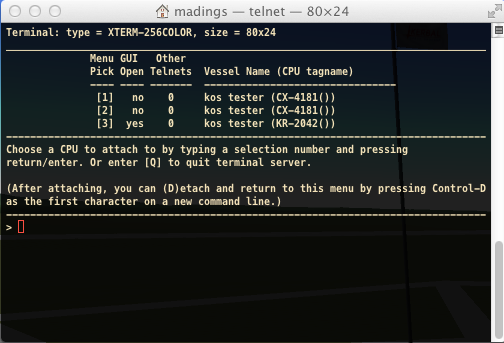
\includegraphics[width=0.750\linewidth]{telnet_welcomemenu.png}
\caption{The welcome menu, shown here in a Mac OSX terminal.}\end{figure}
\begin{enumerate}
\setcounter{enumi}{4}
\item {} 
\textbf{Pick a CPU.}  Pick one of the CPU's listed by typing its number and hitting enter.

\item {} 
Your telnet is now connected to the server and should behave as the terminal for
that CPU.  You can type commands and do what you like, the same as if you had been
directly on its window.

\item {} 
See the section labeled {\hyperref[general/telnet:special-keys]{\emph{Special Keys}}} to see how to use the keyboard from your
telnet client.

\item {} 
It is possible to have multiple terminals hooked up to the same in-game CPU.  They
will all behave as clones of each other, each being an equal ``first citizen''.
(For example a pair of people could execute the ``stage.'' command by having one
of them type ``st'', then the other types ``age'', followed by the first person
typing ''.'' and the return key.)  All the keyboards and all the screens are
slaved together to be equal.  You can view the in-game gui terminal while
somebody is typing on a telnet temrinal.

\item {} 
In order to make the terminals act as clones of each other, the game will attempt
to keep them all the same size.  If you resize your telnet client window, it should
cause the in-game window to change size to match.  (If your terminal type is XTERM,
then the same thing works in reverse.  If it's VT100 then it doesn't.)

\end{enumerate}

\begin{notice}{warning}{Warning:}
Certain implementations of the xterm terminal emulation and the telnet client have
created a strange unending cascade of terminal resizes when you have two different
telnet clients connected to the same GUI terminal and one of them is dragged to a
new size.  Because some implementations don't wait until they're done resizing to
report their new size through telnet and instead report their intermediate sizes as
they are being stretched, the attempt to keep them the same size causes them to
effectively ``argue'' back and forth with each other, constantly changing each
other's size.   If you experience this problem (your terminal window will be
flipping back and forth between two different sizes, resizing itself over and over
again in a neverending loop), you can try to get out of it by issuing a hardcoded
command to set the terminal size, such as:

\begin{Verbatim}[commandchars=\\\{\}]
\PYG{n}{SET} \PYG{n+nl}{TERMINAL}\PYG{p}{:}\PYG{n}{WIDTH} \PYG{n}{TO} \PYG{l+m+mf}{50.}
\end{Verbatim}

Doing this should force all the connected telnet XTERM windows to stop arguing with
each other about what the size is, and get them synced up again.
\end{notice}
\begin{enumerate}
\setcounter{enumi}{9}
\item {} 
At any time you may disconnect your telnet client from the terminal by hitting
control-D as the first character of a new line.  This will bring you back to
the telnet welcome menu again.

\end{enumerate}


\subsection{Special Keys}
\label{general/telnet:special-keys}
The following keys have special meaning in the telnet session:
\begin{description}
\item[{Control-L}] \leavevmode
\textbf{Force refresh} Pressing Control-L forces the kOS telnet server to
redraw your whole screen for you from scratch.  This is useful if
you encounter strange line noise, interrupted messages, or for
just any occasion where you suspect the screen isn't being drawn
correctly.  Pressing control-L will ensure your display gets
fully re-synced with what's in the buffer in memory for the
terminal.

\item[{Control-C}] \leavevmode
\textbf{interrupt process} This is the same meaning as control-C in the normal
GUI terminal - it breaks the program execution.  The reason it gets a special
mention here is that it also causes a flush of all the pending input you may
have typed ahead in the queue.  If you've been typing blindly ahead, and then
hit Control-C, it will erase your typed-ahead keys as it sends the interrupt
to the server.  This is deliberate, and typical practice for an interrupt
character sent over a remote shell setting.

\item[{Control-D}] \leavevmode
\textbf{detach} If you hit control-D as the first character of a new line, it will
detach your telnet session from the CPU and return you to the welcome menu.

\item[{Cursor Keys}] \leavevmode
\textbf{should be mapped} If your terminal has identified itself as one of the known
types that kOS supports, it should understand your arrow keys as arrow keys.
If you see the text ``{[}A'' when you type up-arrow, or ``{[}C'' when you type right-arrow,
this is a clue that kOS didn't recognize your terminal type properly.

\item[{Other Keys}] \leavevmode
\textbf{might be mapped} Some keys like the Del (to the right), Home, and End keys are
often not mapped correctly in some terminal emulator programs.  If you have
trouble using HOME and END, you can try Control-A and Control-E as alternates for
Home and End.

\item[{Control-A}] \leavevmode
\textbf{home} This is an alternate way to press the ``home'' key, just in case your terminal
emulation isn't sending the officially understood terminal code for it.

\item[{Control-E}] \leavevmode
\textbf{end} This is an alternate way to press the ``end'' key, just in case your terminal
emulation isn't sending the officially understood terminal code for it.

\item[{Control-H}] \leavevmode
\textbf{backspace} This is an alternate way to press the ``backspace'' key, just
in case your terminal emulation isn't sending the officially understood
terminal code for it.

\item[{Control-M}] \leavevmode
\textbf{Return} This is an alternate way to press the ``enter'' or ``return'' key,
just in case your terminal emulation isn't sending the officially understood
terminal code for it.

\end{description}


\subsection{HOWTO: Putty client}
\label{general/telnet:howto-putty-client}
(These instructions assume you use the default kOS Telnet server settings, of
the loopback address 127.0.0.1, and port number 5410.  If you've changed those
settings then alter the numbers you see here accordingly.)
\begin{enumerate}
\item {} 
Run KSP, and get it into a scene where there exists a vessel
with at least one kOS CPU loaded into it.

\item {} 
Run Putty.

\item {} 
On the first dialog you see, click the \emph{Telnet} radio-button selection.

\item {} 
Type in the number 127.0.0.1 in the large blank above the radio
buttons that is labeled \emph{``Host Name (or IP address)''}.

\item {} 
Type in the number 5410 in the smaller blank to the right of it
that is labeled \emph{``Port''}.

\item {} 
At the bottom of the screen, select the radio button labeled
\emph{``Never''} under \emph{``Close window on exit''}.

\item {} 
Click the \emph{Open} button to connect to the server.

\end{enumerate}

(You can also save these settings under a name for later re-use.)

Step 6 is important.  Without it, Putty would just make the window disappear any
time there's a problem, making it very hard to diagnose because you can't see what
message the server was sending back to you just before the window went away.


\subsection{HOWTO: Command-line client}
\label{general/telnet:howto-command-line-client}\begin{figure}[htbp]
\centering
\capstart

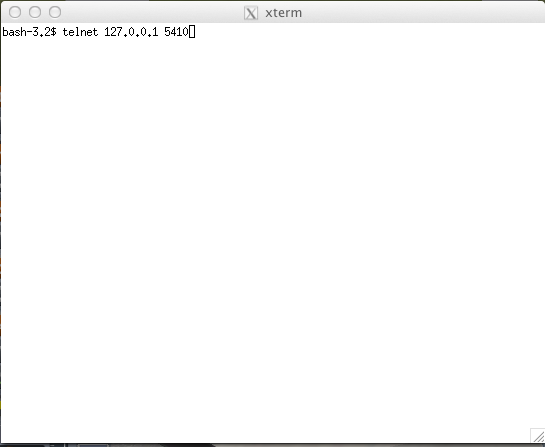
\includegraphics[width=0.750\linewidth]{telnet_xterm.png}
\caption{Showing the use of telnet in an x-term window.}\end{figure}
\begin{figure}[htbp]
\centering
\capstart

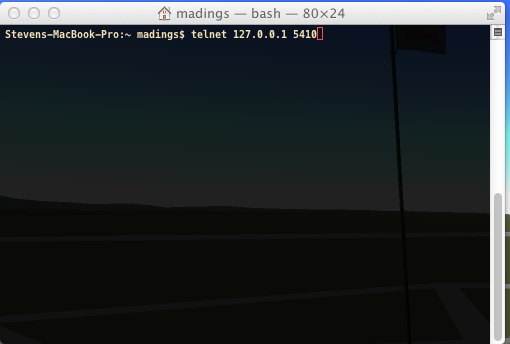
\includegraphics[width=0.750\linewidth]{telnet_macterminal.png}
\caption{Showing the use of telnet in a Mac OSX terminal.}\end{figure}

(These instructions assume you use the default kOS Telnet server settings, of
the loopback address 127.0.0.1, and port number 5410.  If you've changed those
settings then alter the numbers you see here accordingly.)
\begin{enumerate}
\item {} 
Run KSP, and get it into a scene where there exists a vessel with
at least one
kOS CPU loaded into it.

\item {} 
Open a command shell window that either \emph{IS} xterm, or emulates xterm.  For
OSX, the default command shell should work fine.  For Linux, you should
actually have the xterm program itself installed that you can use.

\item {} 
At the shell prompt in that window, enter the command:

\begin{Verbatim}[commandchars=\\\{\}]
\PYG{n}{telnet} \PYG{l+m+mf}{127.0}\PYG{l+m+mf}{.0}\PYG{l+m+mf}{.1} \PYG{l+m+mi}{5410}
\end{Verbatim}

\end{enumerate}


\subsection{HOWTO: Other client}
\label{general/telnet:howto-other-client}\begin{enumerate}
\item {} 
Set the IP address to 127.0.0.1 using whatever means the program has for it.

\item {} 
Set the port number to 5410 using whatever means the program has for it.

\item {} 
Set the terminal to XTERM emulation mode if it has it, or VT100 mode as a
less good, but still perhaps workable option.

\item {} 
Run the terminal.

\end{enumerate}


\subsection{Security}
\label{general/telnet:security}
The telnet protocol performs no encryption of its data, and as such any attempt
at securing the system using a name/password combination would have been
utterly pointless.  Rather than provide a false sense of security that's not
really there, we decided to make it obvious that there's no security by not
even implementing a name and password for connecting to the kOS telnet server.

The purpose is to make it clear that if you want to open up your kOS telnet
server, you need to be careful about how you do it.

The default settings that kOS ships with restricts your kOS telnet server to
only operating on the loopback address (127.0.0.1) so that you won't accidentally
open anything up to the public without thinking about it and making a conscious
decision to do so.  If you don't know what that means, it means this:
Any server that runs on the magic special address 127.0.0.1, known as ``loopback'',
is incapable of taking connections from other computers besides itself.

In order to allow your kOS telnet server to take connections from other
computers, you will typically need to do one of two things:

Either turn off the CONFIG:LOOPBACK option in your kOS install and then
restart your telnet server (turn it off and on again using the button on the
control panel), or (much better), set up a remote ssh tunnel that will map
from your current machine's loopback address on the port number of your server to
some remote other computer you want to connect from, to a port on it.  The ssh
tunnel is the preferred method, but describing how to set one up is beyond the
scope of this document.  You can read more
\href{http://realprogrammers.com/how\_to/set\_up\_an\_ssh\_tunnel\_with\_putty.html}{For windows} or
\href{http://www.cyberciti.biz/faq/set-up-ssh-tunneling-on-a-linux-unix-bsd-server-to-bypass-nat/}{For UNIX (both Mac and Linux)}.

Example: Let's say you have a remote Unix machine you'd like to enable logins from,
from there and nowhere else.  You can forward from your own machine's
127.0.0.1, port 5410, to the remote machine's, oh let's say 127.0.0.1, port 54100.
Then anyone on the remote machine could telnet to ITS 127.0.0.1, port 54100 and
end up talking to your machine's port 5410 on its loopback address.

\textbf{Port forwarding}

If you opt to turn off the loopback-only mode on your kOS telnet server, then you
will probably also, if you have a typical home network setup, need to enable
port forwarding on your router if you want people from outside your house to
connect to it.  (Again, think about the implications of doing so before you do it).
This is a topic beyond the scope of this document, but help can be found out on
the web for it.  Search for ``port forward home router''.  (It is probably also a
good idea to include the make \& model number of your router device in your search
terms, to get a nicely narrowed result that's exactly what you need.)

\textbf{Why not ssh?}

The original plan for kOS was to include an ssh server
instead of a telnet server.  However this proved problematic as open source
solutions in C\# for the server-side of ssh were hard to come by (there's several
for the client side only, and plenty of server-side code that's not in C\#), and
implementing the entire server side of the ssh protocol from scratch is a
daunting task that would have taken too much time away from other development
of kOS.  (While implementing from scratch the server side of the older, simpler
telnet protocol, while still work, was more doable).


\subsection{Homemade telnet clients}
\label{general/telnet:homemade-telnet-clients}
This section is only of interest to hobbyists making Kerbal console hardware rigs
and software developers trying to make interface mods that pretend to be
kOS terminals.  If you are neither of those two, then don't worry if this section
looks like gibberish to you.  It can be skipped.

\textbf{TELNET PROTOCOL}

If you wish to make your own homemade telnet client and connect it up to the
kOS telnet server, the following is the required subset of the telnet protocol
that your telnet client must speak, and the terminal requirements it must
fulfill:
\begin{enumerate}
\item {} 
It must suppress local character echoing, and enter character-at-a-time mode,
by implementing both the ECHO negotiation
\href{http://www.networksorcery.com/enp/rfc/rfc857.txt}{described by RFC857}, and
the SUPPRESS GO AHEAD negotiation
\href{http://www.networksorcery.com/enp/rfc/rfc858.txt}{described by RFC858}. These are
used in the following way:  Your client must NOT ECHo (letting the server do it),
and your client must suppress go-ahead messages (allowing real-time back-and-forth).

\item {} 
It must implement the underlying DO/DONT and WILL/WONT, and SB/SE infrastructure of
the main \href{http://www.networksorcery.com/enp/rfc/rfc854.txt}{telnet RFC854}.  It must
send break (ctrl-C) as the IP interrupt process command (byte 255 followed by 244).
kOS does not use much of the negotiations of the protocol mentioned on RFC854, other
than those that are necessary to enable the other ones mentioned here.

\item {} 
It must implement the Terminal-Type option
\href{http://www.networksorcery.com/enp/rfc/rfc1091.txt}{described by RFC1091}.
Furthermore, as of this writing, kOS only knows how to understand two terminal types,
``XTERM'', and ``VT100''.  If your terminal type is identified as anything else, kOS
may deny your connection, or at the very least just not work right.  Even terminals
that are capable of emulating XTERM or VT100 commands won't work right if they
don't identify themselves as XTERM or VT100.  kOS does not know how to guess what
emulation mode to enter if it doesn't recognize your terminal type string.

\item {} 
It must implement the NAWS, Negotiate About Terminal Size option, as
\href{http://www.networksorcery.com/enp/rfc/rfc1073.txt}{described by RFC1073}.
kOS uses this to decide how to size its mental image of your terminal to match
your terminal's real size.  Note that this negotiation is one-way.  Your client
can use it to tell the server about its size, but the server can't use it to
tell your client to change its size.  Instead if your client can respond to changing
sizes at the behest of the server, it must do so through terminal escape code
characters sent back to it on the stream, above the telnet protocol layer itself.
(For example, if you identify as XTERM, you will be sent the XTERM escape code
pattern ESC {[} 8 ; \emph{height} ; \emph{width} t, which is the XTERM escape code for setting
the terminal size.)  This is because the telnet protocol was never written to
accommodate the concept of server-initiated resizes.

\end{enumerate}

Making a telnet client from scratch that actually follows protocol may be a complex
enough task that the smarter solution is to just use an existing telnet program, if
you are trying to create some sort of hardware rig.  These days a small cheap
mini-hardware implementation of Linux should be doable, and could include the
telnet client installed in it for very little storage cost.

\textbf{TERMINAL EMULATION}

As of right now, the terminal emulation of kOS only really supports XTERM
or VT100 well, however the infrastructure is in place to support modifications
to map to other terminal types.  If you want to try a hand at adding the
terminal emulation for a currently unsupported terminal, you'd do it
by subclassing the kOS.UserIO.TerminalUnicodeMapper class.  You can
look at kOS.UserIO.TerminalXtermMapper as a sample to see what you need
to do.

If you have a project where you want to just work with the terminal
codes already supported, then these are the subset you need to support:
\begin{description}
\item[{\emph{ASCII}}] \leavevmode
The following terms should have their normal ASCII meaning:

\item[{0x08 (control-H)}] \leavevmode
backspace key

\item[{0x0d (control-M)}] \leavevmode
Return key.  On output it means go to left edge but don't go down a line.
A typical eoln needs to occur using its ASCII standard of both a
return character 0x0d AND a linefeed character 0x0a

\item[{0x0a (control-J)}] \leavevmode
On output it means go to go down a line but don't go to the left edge
A typical eoln needs to occur using its ASCII standard of both a
return character 0x0d AND a linefeed character 0x0a

\end{description}

\textbf{Terminal codes:} \emph{The following terms should have their VT100/XTERM meaning}
\begin{description}
\item[{Left-Arrow}] \leavevmode
ESC {[} D  \emph{-- both on input and on output}

\item[{Right-Arrow}] \leavevmode
ESC {[} C  \emph{-- both on input and on output}

\item[{Up-Arrow}] \leavevmode
ESC {[} A  \emph{-- both on input and on output}

\item[{Down-Arrow}] \leavevmode
ESC {[} B  \emph{-- both on input and on output}

\item[{Home-key}] \leavevmode
ESC {[} 1 \textasciitilde{}  \emph{-- input only}

\item[{End-key}] \leavevmode
ESC {[} 4 \textasciitilde{}  \emph{-- input only}

\item[{Delete-to-the-right-key}] \leavevmode
ESC {[} 3 \textasciitilde{}  \emph{-- input only}

\item[{PageUp-key}] \leavevmode
ESC {[} 5 \textasciitilde{}  \emph{-- input only}

\item[{PageDown-key}] \leavevmode
ESC {[} 6 \textasciitilde{}  \emph{-- input only}

\item[{Move-to-home-of-screen-upper-left}] \leavevmode
ESC {[} H  \emph{-- output only}

\item[{Move-to-end-of-line}] \leavevmode
ESC {[} F  \emph{-- output only}

\item[{Teleport-cursor-to-coordinate}] \leavevmode
ESC {[} \emph{row} ; \emph{col} H   \emph{-- output only: rows and cols start counting at 1, not 0}

\item[{Clearscreen}] \leavevmode
ESC {[} 2 J  \emph{-- output only}

\item[{Scroll-screen-up-one-line-keeping-cursor-where-it-is}] \leavevmode
ESC {[} S  \emph{-- output only}

\item[{Scroll-screen-down-one-line-keeping-cursor-where-it-is}] \leavevmode
ESC {[} T  \emph{-- output only}

\item[{Delete-to-the-left-of-cursor-ie-backspace}] \leavevmode
ESC {[} K  \emph{-- output only}

\item[{Delete-at-the-cursor-toward-the-right}] \leavevmode
ESC {[} 1 K  \emph{-- output only}

\end{description}

\textbf{XTERM codes:} \emph{The following codes are for the XTERM emulation only}
\begin{description}
\item[{Server-telling-client-to-resize-screen}] \leavevmode
ESC {[} 8 ; \emph{newheight} ; \emph{newwidth} t  \emph{-- The height/width are in chars}

\item[{Server-telling-client-to-change-window-title}] \leavevmode
ESC {]} 2 ; \emph{title string} BEL  \emph{-- where BEL is the character normally
used to mean beep: control-G or 0x07.  But in this context it just marks
the end of the title and shouldn't cause a beep.}
Note this is NOT a typo that it uses a right-square-bracket (``{]}'') here where
all the other codes used a left-square-bracket (``{[}'').  That's actually
how the xterm control sequence for this really looks.

\end{description}

Any value not mentioned in the list above might still get sent, but you
should be able to capture and ignore it.


\section{Files and Volumes}
\label{general/volumes:files-and-volumes}\label{general/volumes::doc}\label{general/volumes:volumes}
Using the COPY, SWITCH, DELETE, and RENAME commands, you can manipulate the archive and the volumes as described in the {\hyperref[commands/files:files]{\emph{\DUspan{}{File I/O page}}}}. But before you do that, it's useful to know how kOS manages the archive and the volumes, and what they mean.
\setbox0\vbox{
\begin{minipage}{0.95\linewidth}
\begin{itemize}
\item {} 
\phantomsection\label{general/volumes:id1}{\hyperref[general/volumes:script-files]{\emph{Script Files}}}

\item {} 
\phantomsection\label{general/volumes:id2}{\hyperref[general/volumes:file-storage-behind-the-scenes]{\emph{File Storage Behind the Scenes}}}

\item {} 
\phantomsection\label{general/volumes:id3}{\hyperref[general/volumes:you-can-get-more-space-by-paying-extra-cost-in-money-and-mass]{\emph{You can get more space by paying extra cost in money and mass}}}

\item {} 
\phantomsection\label{general/volumes:id4}{\hyperref[general/volumes:multiple-volumes-on-one-vessel]{\emph{Multiple Volumes on One Vessel}}}

\item {} 
\phantomsection\label{general/volumes:id5}{\hyperref[general/volumes:naming-volumes]{\emph{Naming Volumes}}}

\item {} 
\phantomsection\label{general/volumes:id6}{\hyperref[general/volumes:archive]{\emph{Archive}}}

\end{itemize}
\end{minipage}}
\begin{center}\setlength{\fboxsep}{5pt}\shadowbox{\box0}\end{center}

\begin{notice}{warning}{Warning:}
\DUspan{versionmodified}{Changed in version 0.15: }\textbf{Archive location and file extension change}

The Archive where KerboScript files are kept has been changed from \code{Plugins/PluginData/Archive} to \code{Ships/Script}, but still under the top-level \textbf{KSP} installation directory. The file name extensions have also changes from \code{.txt} to \code{.ks}.
\end{notice}


\subsection{Script Files}
\label{general/volumes:script-files}
There is one file per program. You can use the words ``file'' and ``program'' interchangeably in your thinking for the most part. Files are stored in volumes and there can be more than one file in a volume provided there's enough room. Volumes have small storage and there's no way to span a file across two volumes, so the limit to the size of a volume is also effectively a limit to the size of a program.


\subsection{File Storage Behind the Scenes}
\label{general/volumes:file-storage-behind-the-scenes}
In the Archive:
\begin{itemize}
\item {} 
If a file is stored on the volume called ``Archive'' (or volume number
zero to put it another way), then behind the scenes it's really
stored as an actual file, with the extension \code{.ks}, on your
computer (As of right now it's located in \code{Ships/Script} but that
location is likely to change to somewhere in GameData in a future
version.) Each program is a simple text file you can edit with any
text editor, and your edits will be seen immediately by KOS the next
time it tries running that program from the archive volume.

\item {} 
Historical note: older versions of kOS (0.14 and earlier) used the
directory \code{Plugins/PluginData/Archive} for the archive.

\end{itemize}

In any other volume besides Archive:
\begin{itemize}
\item {} 
If a file is stored on any volume other than archive, then behind the
scenes it's stored actually inside the saved game's persistence file
in the section for the KOS part on the vessel.
What's a Volume

\end{itemize}

A Volume is a small unit of disk storage that contains a single hard
drive with very limited storage capacity. It can store more than one
program on it. To simulate the sense that this game takes place at the
dawn of the space race with 1960's and 1970's technology, the storage
capacity of a volume is very limited.

For example, the CX-4181 Scriptable Control System part defaults to only
allowing 1000 bytes of storage.

The byte count of a program is just the
count of the characters in the source code text. Writing programs with
short cryptic variable names instead of long descriptive ones does save
space, although you can also save space by compiling your programs to
KSM files where the variable names are only stored once in the file, but
that's another topic for another page.

Each of the computer parts that kOS supports have their own different default
storage capacity limits for their local volume.  As you get better parts
higher up the tech tree, they come with bigger default size limits.


\subsection{You can get more space by paying extra cost in money and mass}
\label{general/volumes:you-can-get-more-space-by-paying-extra-cost-in-money-and-mass}\begin{figure}[htbp]
\centering

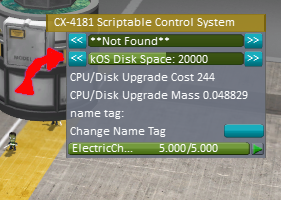
\includegraphics{disk_space_slider.png}
\end{figure}

If you wish to have more disk space on your local volume, and are willing to
pay a little extra cost in money and in mass, you can use the disk space
slider in the vehicle assembly building to increase the limit.

Every part comes with 3 different multiplier options:
\begin{itemize}
\item {} 
1x default size,

\item {} 
2x default size,

\item {} 
4x default size

\end{itemize}

The higher the multiplier the more mass it will
cost you, to represent that you're using old storage technology,
so it costs a lot of mass to have more storage.

The disk size is only settable like this in the assembly building.  Once
you launch a vessel, its volume size is stuck the way it was when you
launched it.


\subsection{Multiple Volumes on One Vessel}
\label{general/volumes:multiple-volumes-on-one-vessel}
Each kOS CX-4181 Scriptable Control System part contains `'`one'`' such
volume inside it.

If you have multiple CX-4181 parts on the same craft, they are assumed
to be networked together on the same system, and capable of reading each
other's hard drives. Their disk drives each have a different Volume, and
by default they are simply numbered 1,2,3, … unless you rename them with
the RENAME command.

For example, if you have two CX-4181's on the same craft, called 1 and
2, with volumes on them called 1 and 2, respectively, it is possible for
CPU 1 to run code stored on volume 2 by just having CPU number 1 issue
the command `'SWITCH TO 2.'`


\subsection{Naming Volumes}
\label{general/volumes:naming-volumes}
It's important to note that if you have multiple volumes on the same
vessel, the numbering conventions for the volumes will differ on
different CPUs. The same volume which was called `2' when one CPU was
looking at it might instead be called `1' when a different CPU is
looking at it. Each CPU thinks of its OWN volume as number `1'.

Therefore using the RENAME command on the volumes is useful when dealing
with multiple CX-4181's on the same vessel, so they all will refer to
the volumes using the same names.


\subsection{Archive}
\label{general/volumes:archive}
The ``archive'' is a special volume that behaves much like any other
volume but with the following exceptions:
\begin{itemize}
\item {} 
It is globally the same even across save games.

\item {} 
The archive represents the large bank of disk storage back at mission
control's mainframe, rather than the storage on an indivdual craft.
While ``Volume 1'' on one vessel might be a different disk than ``Volume
1'' on another vessel, there is only volume called ``archive'' in the
entire solar system. Also, there's only one ``archive'' across all
saved universes. If you play a new campaign from scratch, your
archive in that new game will still have all the files in it from
your previous saved game. This is because behid the scenes it's
stored in the plugin's directory, not the save game directory.

\item {} 
It is infinitely large.

\item {} 
Unlike the other volumes, the archive volume does not have a byte
limit. This is because the mainframe back at home base can store a
lot more than the special drives sent on the vessels - so much so
that it may as well be infinite by comparison.

\item {} 
Files saved there do not revert when you ``revert flight''.

\item {} 
When you revert a flight, you are going back to a previous saved
state of the game, and therefore any disk data on the vessels
themselves also reverts to what it was at the time of the saved game.
Because the archive is saved outside the normal game save, changes
made there are retained even when reverting a flight.

\item {} 
It's not always reachable if you are out in space, unless you have
antennae.

\item {} 
Once a vessel is more than 100,000 meters away from mission control,
by default it cannot access the files on the archive. Commands such
as SWITCH TO , and COPY FROM will fail to work when trying to access
the archive volume while out of range. This can be changed by putting
antennae on the vessel. With enough
antennae it becomes possible
to reach the archive drive from farther away. Using this method it is
possible to alter the software stored on a vessel after launch.

\item {} 
Files in Archive are editable with a text editor directly and they
will have the \code{.ks} extension.

\item {} 
Files in the Archive are stored on your computer in the subdirectory:
\code{Ships/Script}. You can pull them up in a text editor of your
choice and edit them directly, and the KOS Mod will see those changes
in its archive immediately. Files stored in other volumes, on the
other hand, are stored inside the vessel's data in the persistence
file of the saved game and are quite a bit bit harder to edit there.
Editing the files in the Archive directory is allowed and in fact is
an officially accepted way to use the plugin. Editing the section in
a persistence file, on the other hand, is a bad idea and probably
constitutes a form of cheating similar to any other edit of the
persistence file.

\end{itemize}


\section{KerboScript Machine Code}
\label{general/compiling:kerboscript-machine-code}\label{general/compiling:compiling}\label{general/compiling::doc}\setbox0\vbox{
\begin{minipage}{0.95\linewidth}
\begin{itemize}
\item {} 
\phantomsection\label{general/compiling:id1}{\hyperref[general/compiling:compiling-to-a-ksm-file]{\emph{Compiling to a KSM File}}}

\item {} 
\phantomsection\label{general/compiling:id2}{\hyperref[general/compiling:how-to-use-ksm-files]{\emph{How to Use KSM Files}}}

\item {} 
\phantomsection\label{general/compiling:id3}{\hyperref[general/compiling:default-file-naming-conventions]{\emph{Default File Naming Conventions}}}

\item {} 
\phantomsection\label{general/compiling:id4}{\hyperref[general/compiling:downsides-to-using-ksm-files]{\emph{Downsides to Using KSM Files}}}

\item {} 
\phantomsection\label{general/compiling:id5}{\hyperref[general/compiling:more-reading-and-fiddling-with-your-bits]{\emph{More Reading and Fiddling with Your Bits}}}

\end{itemize}
\end{minipage}}
\begin{center}\setlength{\fboxsep}{5pt}\shadowbox{\box0}\end{center}


\subsection{Compiling to a KSM File}
\label{general/compiling:compiling-to-a-ksm-file}
When you run your Kerboscript programs, behind the scenes they get compiled into a form in memory that runs much smoother but at the same time is quite hard for a Kerbal to read and understand. The actual computer hardware built by your friends at Compotronix incorporated actually run the program using these tiny instructions called ``opcodes''. In the early days of room-sized computers before we were able to get them down to the compact size of just a meter or so across, all programmers had to use this difficult system, referred to as ``machine language''. Ah, those were heady days, but they were hard.

The commands you actually write when you say something like \code{SET X TO 1.0.} are really a euphemism for these ``machine language'' opcodes under the surface.

When you try to ``RUN'' your script, the first thing that kOS does is transform your script into this ancient and arcane ``machine language'' form, storing it in its memory, and from then on it runs using that.

This process of transforming your script into Machine Language, or ``ML'' is called ``Compiling''.

The ``RUN'' command does this silently, without telling you. This is why you may have noticed the universe slightly stutter for a moment when you first run your program. Compiling is hard work for the universe to do.


\subsubsection{Why Do I Care?}
\label{general/compiling:why-do-i-care}
\begin{notice}{warning}{Warning:}
This is an experimental feature.
\end{notice}

The reason it matters is this: Although once it's loaded into memory and running, these opcodes actually have a lot of baggage and take up a lot of space, when they're stored passively on the disk not doing anything, they can be smaller than your script programs are. For one thing, they don't care about your comments (only other Kerbals reading your script do), and they don't care about your indenting (only other Kerbals reading your script do).

So, given that the compiled ``ML'' codes are the only thing your program really needs to be run, why not just store THAT instead of storing the entire script, and then you can put the ML files on your remote probes instead of putting the larger script files on them.

And THAT is the purpose of the COMPILE command.

It does some, but not all, of the compiling work that the RUN command does, and then stores the results in a file that you can run instead of running the original script.

The output of the COMPILE command is a file in what we call KSM format.

KSM stands for ``KerboScript Machine code'', and it has nearly the same information the program will have when it's loaded and running, minus a few extra steps about relocating it in memory.


\subsection{How to Use KSM Files}
\label{general/compiling:how-to-use-ksm-files}
Let's say that you have 3 programs your probe needs, called:
\begin{itemize}
\item {} 
myprog1.ks

\item {} 
myprog2.ks

\item {} 
myprog3.ks

\end{itemize}

And that myprog1 calls myprog2 and myprog3, and you normall would call the progam this way:

\begin{Verbatim}[commandchars=\\\{\}]
\PYG{n}{SWITCH} \PYG{n}{TO} \PYG{l+m+mf}{1.}
\PYG{n}{COPY} \PYG{n}{myprog1} \PYG{n}{from} \PYG{n}{ARCHIVE}\PYG{p}{.}
\PYG{n}{COPY} \PYG{n}{myprog2} \PYG{n}{from} \PYG{n}{ARCHIVE}\PYG{p}{.}
\PYG{n}{COPY} \PYG{n}{myprog3} \PYG{n}{from} \PYG{n}{ARCHIVE}\PYG{p}{.}
\PYG{n}{RUN} \PYG{n}{myprog1}\PYG{p}{(}\PYG{l+m+mi}{1}\PYG{p}{,}\PYG{l+m+mi}{2}\PYG{p}{,}\PYG{l+s}{\PYGZdq{}}\PYG{l+s}{hello}\PYG{l+s}{\PYGZdq{}}\PYG{p}{)}\PYG{p}{.}
\end{Verbatim}

Then you can put just the compiled KSM versions of them on your vessel and run it this way:

\begin{Verbatim}[commandchars=\\\{\}]
\PYG{n}{SWITCH} \PYG{n}{TO} \PYG{n}{ARCHIVE}\PYG{p}{.}

\PYG{n}{COMPILE} \PYG{n}{myprog1}\PYG{p}{.}\PYG{n}{ks} \PYG{n}{to} \PYG{n}{myprog1}\PYG{p}{.}\PYG{n}{ksm}\PYG{p}{.}
\PYG{n}{COPY} \PYG{n}{myprog1}\PYG{p}{.}\PYG{n}{ksm} \PYG{n}{to} \PYG{l+m+mf}{1.}

\PYG{n}{COMPILE} \PYG{n}{myprog2}\PYG{p}{.} \PYG{c+c1}{// If you leave the arguments off, it assumes you are going from .ks to .ksm}
\PYG{n}{COPY} \PYG{n}{myprog2}\PYG{p}{.}\PYG{n}{ksm} \PYG{n}{to} \PYG{l+m+mf}{1.}

\PYG{n}{COMPILE} \PYG{n}{myprog3}\PYG{p}{.} \PYG{c+c1}{// If you leave the arguments off, it assumes you are going from .ks to .ksm}
\PYG{n}{COPY} \PYG{n}{myprog2}\PYG{p}{.}\PYG{n}{ksm} \PYG{n}{to} \PYG{l+m+mf}{1.}

\PYG{n}{SWITCH} \PYG{n}{TO} \PYG{l+m+mf}{1.}
\PYG{n}{RUN} \PYG{n}{myprog1}\PYG{p}{(}\PYG{l+m+mi}{1}\PYG{p}{,}\PYG{l+m+mi}{2}\PYG{p}{,}\PYG{l+s}{\PYGZdq{}}\PYG{l+s}{hello}\PYG{l+s}{\PYGZdq{}}\PYG{p}{)}\PYG{p}{.}
\end{Verbatim}


\subsection{Default File Naming Conventions}
\label{general/compiling:default-file-naming-conventions}
When you have both a .ks and a .ksm file, the RUN command allows you to specify which one you meant explicitly, like so:

\begin{Verbatim}[commandchars=\\\{\}]
\PYG{n}{RUN} \PYG{n}{myprog1}\PYG{p}{.}\PYG{n}{ks}\PYG{p}{.}
\PYG{n}{RUM} \PYG{n}{myprog1}\PYG{p}{.}\PYG{n}{ksm}\PYG{p}{.}
\end{Verbatim}

But if you just leave the file extension off, and do this:

\begin{Verbatim}[commandchars=\\\{\}]
\PYG{n}{RUN} \PYG{n}{myprog1}\PYG{p}{.}
\end{Verbatim}

Then the RUN command will first try to run a file called ``myprog1.ksm'' and if it cannot find such a file, then it will try to run one called ``myprog1.ks''.

In this way, if you decide to take the plunge and attempt the use of KSM files, you shouldn't have to change the way any of your scripts call each other, provided you just used versions of the filenames without mentioning the file extensions.


\subsection{Downsides to Using KSM Files}
\label{general/compiling:downsides-to-using-ksm-files}\begin{enumerate}
\item {} 
Be aware that if you use this feature, you do lose the ability to have the line of code printed out for you when the kOS computer finds an error in your program. It will still tell you what line number the error happened on, but it cannot show you the line of code. Just the number.

\item {} 
Know that you cannot view the program inside the in-game editor anymore when you do this. A KSM file will not appear right in the editor. It requires a magic tool called a ``hex editor'' to properly see what's happening inside the file.

\item {} 
\textbf{The file isn't always smaller}. There's a threshold at which the KSM file is actually bigger than the source KS file. For large KS files, the KSM file will be smaller, but for short KS files, the KSM file will be bigger, because there's a small amount of overhead they have to store that is only efficient if the data was large enough.

\end{enumerate}


\subsection{More Reading and Fiddling with Your Bits}
\label{general/compiling:more-reading-and-fiddling-with-your-bits}
So, if you are intrigued by all this and want to see how it all \emph{REALLY} works under the hood, Computronix has deciced to make \href{https://github.com/KSP-KOS/KOS/blob/develop/src/kOS.Safe/Compilation/CompiledObject-doc.md}{internal document MLfile-zx1/a} on the basic plan of the ML file system open for public viewing, if you are one of those rare Kerbals that enjoys fiddling with your bits. No, not THOSE kind of bits, the computery kind!


\section{The Name Tag System}
\label{general/nametag:nametag}\label{general/nametag::doc}\label{general/nametag:the-name-tag-system}\begin{figure}[htbp]
\centering

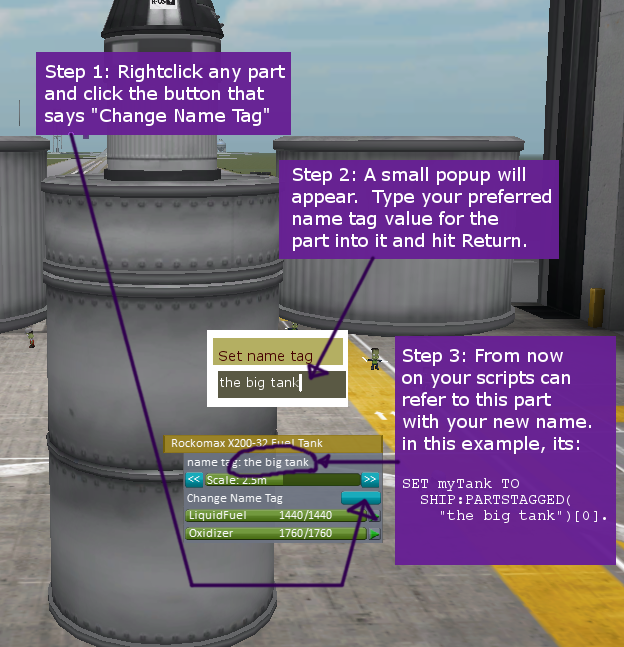
\includegraphics{nametag.png}
\end{figure}

One useful thing to do is to be able to give parts on a craft your own chosen names that you can use to get a reference to the parts, utterly bypassing the naming schemes used by KSP, and ignoring the complex part tree system. The Name Tag system was designed to make it possible for you to just give any part on a craft whatever arbitrary name you feel like.
\setbox0\vbox{
\begin{minipage}{0.95\linewidth}
\begin{itemize}
\item {} 
\phantomsection\label{general/nametag:id1}{\hyperref[general/nametag:giving-a-part-a-name]{\emph{Giving a Part a Name}}}

\item {} 
\phantomsection\label{general/nametag:id2}{\hyperref[general/nametag:cloning-with-symmetry]{\emph{Cloning with Symmetry}}}

\item {} 
\phantomsection\label{general/nametag:id3}{\hyperref[general/nametag:where-is-it-saved]{\emph{Where is it saved?}}}

\item {} 
\phantomsection\label{general/nametag:id4}{\hyperref[general/nametag:examples-of-using-the-name]{\emph{Examples of Using the Name}}}

\end{itemize}
\end{minipage}}
\begin{center}\setlength{\fboxsep}{5pt}\shadowbox{\box0}\end{center}


\subsection{Giving a Part a Name}
\label{general/nametag:giving-a-part-a-name}\begin{enumerate}
\item {} 
Right click on any part. **You can do this in either the editor
VAB/SPH,
or during flight.** It is more useful to do beforehand when making
the
craft, but you can do it in the midst of a flight, which is useful
for
experimenting and testing.

\item {} 
Click the ``change name tag'' button. A small text pop-up will appear
with the ability to type a name for the part. Type any value you
like. In the example picture here, the value ``the big tank'' was typed
in.

\item {} 
From now on this part can be retrieved using either the :PARTSDUBBED
or
the :PARTSTAGGED methods of the vessel, as described
on the Vessel Page

\end{enumerate}


\subsection{Cloning with Symmetry}
\label{general/nametag:cloning-with-symmetry}
If you name a part in the editor \emph{first}, and then remove it from the
vessel and place it again with symmetry, all the symmetry copies of the
part will get the same nametag cloned to them. This is not an error. It
is allowed to give the same nametag to more than one part. If you do
this,
it just means that the :PARTSTAGGED or :PARTSDUBBED methods will return
lists containing more than one part.

If you want each part in a symmetrical group to get a unique nametag,
you
can change their names one at a time after you've placed the parts.


\subsection{Where is it saved?}
\label{general/nametag:where-is-it-saved}
If you add a nametag to a part in the editor (VAB or SPH), then that
nametag will get saved inside the craft file for that vessel design.
All new instances of that craft design that you launch will get the
same nametag configuration on them.

On the other hand, if you added a nametag to a part after the vessel
was launched, during flight or on the launchpad, then that nametag
will only be attached to that part on \emph{that one instance} of the
vessel. Other copies of the same design won't have the name. In this
case the name is saved inside the saved game's persistence file, but
not in the editor's craft design file.


\subsection{Examples of Using the Name}
\label{general/nametag:examples-of-using-the-name}
\begin{Verbatim}[commandchars=\\\{\}]
\PYG{c+c1}{// Only if you expected to get}
\PYG{c+c1}{// exactly 1 such part, no more, no less.}
\PYG{n}{SET} \PYG{n}{myPart} \PYG{n}{TO} \PYG{n+nl}{SHIP}\PYG{p}{:}\PYG{n}{PARTSDUBBED}\PYG{p}{(}\PYG{l+s}{\PYGZdq{}}\PYG{l+s}{my nametag here}\PYG{l+s}{\PYGZdq{}}\PYG{p}{)}\PYG{p}{[}\PYG{l+m+mi}{0}\PYG{p}{]}\PYG{p}{.}

\PYG{c+c1}{// OR}

\PYG{c+c1}{// Only if you expected to get}
\PYG{c+c1}{// exactly 1 such part, no more, no less.}
\PYG{n}{SET} \PYG{n}{myPart} \PYG{n}{TO} \PYG{n+nl}{SHIP}\PYG{p}{:}\PYG{n}{PARTSTAGGED}\PYG{p}{(}\PYG{l+s}{\PYGZdq{}}\PYG{l+s}{my nametag here}\PYG{l+s}{\PYGZdq{}}\PYG{p}{)}\PYG{p}{[}\PYG{l+m+mi}{0}\PYG{p}{]}\PYG{p}{.}

\PYG{c+c1}{// Handling the case of more than}
\PYG{c+c1}{// one part with the same nametag,}
\PYG{c+c1}{// or the case of zero parts with}
\PYG{c+c1}{// the name:}
\PYG{n}{SET} \PYG{n}{allSuchParts} \PYG{n}{TO} \PYG{n+nl}{SHIP}\PYG{p}{:}\PYG{n}{PARTSDUBBED}\PYG{p}{(}\PYG{l+s}{\PYGZdq{}}\PYG{l+s}{my nametag here}\PYG{l+s}{\PYGZdq{}}\PYG{p}{)}\PYG{p}{.}

\PYG{c+c1}{// OR}

\PYG{n}{SET} \PYG{n}{allSuchParts} \PYG{n}{TO} \PYG{n+nl}{SHIP}\PYG{p}{:}\PYG{n}{PARTSTAGGED}\PYG{p}{(}\PYG{l+s}{\PYGZdq{}}\PYG{l+s}{my nametag here}\PYG{l+s}{\PYGZdq{}}\PYG{p}{)}\PYG{p}{.}

\PYG{c+c1}{// Followed by using the list returned:}
\PYG{n}{FOR} \PYG{n}{onePart} \PYG{n}{IN} \PYG{n}{allSuchParts} \PYG{p}{\PYGZob{}}
  \PYG{c+c1}{// do something with onePart here.}
\PYG{p}{\PYGZcb{}}
\end{Verbatim}

For more details on how this system works see the {\hyperref[general/parts_and_partmodules:parts-and-partmodules]{\emph{\DUspan{}{Parts and PartModules Section}}}}.


\section{Ship Parts and PartModules}
\label{general/parts_and_partmodules:ship-parts-and-partmodules}\label{general/parts_and_partmodules::doc}\label{general/parts_and_partmodules:parts-and-partmodules}
As of v0.15, kOS has introduced the ability to access the functionality of Parts' actions, and right-click context menus. However, to understand how to use them it is necessary to first understand a little bit about the structure of parts in a vessel in Kerbal Space Program.

In Kerbal Space Program, a Vessel is a collection of Parts arranged in a tree Structure. In kOS, you can access the parts one of two ways:


\subsection{Tutorial}
\label{general/parts_and_partmodules:tutorial}
If you prefer the tutorial approach to learning, the following links will walk you through a specific pair of tasks to introduce you to this system. If you prefer a methodical reference approach, skip the tutorials and read on, then come back to the tutorials afterward.

TODO: PUT LINKS POINTING TO A TUTORIAL WALKING THROUGH WHAT THIS IS TEACHING.

THERE NEEDS TO BE TWO TUTORIALS MINIMUM:
\begin{enumerate}
\item {} 
A Tuturial made on an ONLY STOCK (other than kOS of course) install, using only STOCK parts to do something interesting.

\item {} 
A Tutorial more complex showing that this can be used with mods too, probably the Leg Leveller example from the teaser video, but with the code updated to use the newer part query methods.

\end{enumerate}


\subsection{Parts}
\label{general/parts_and_partmodules:parts}
\begin{notice}{note}{Note:}
\textbf{The short and quick thing to remember}

If you only remember one technique, it should be using the \code{Part:PARTSDUBBED} method described down below. It's the most useful one that covers all the other cases.
\end{notice}


\subsubsection{Accessing the parts by various naming systems}
\label{general/parts_and_partmodules:accessing-the-parts-by-various-naming-systems}
Any time you have a vessel variable, you can use these suffixes to get lists of parts on it by their names using several different naming schemes:

\textbf{Part Tag}: A part's \emph{tag} is whatever custom name you have given it using the nametag system described here. This is probably the best naming convention to use because it lets you make up whatever name you like for the part and use it to pick the parts you want to deal with in your script.

\textbf{Part Title}: A part's \emph{title} is the name it has inside the GUI interface on the screen that you see as the user.

\textbf{Part Name}: A part's \emph{name} is the name it is given behind the scenes in KSP. It never appears in the normal GUI for the user to see, but it is used in places like Part.cfg files, the saved game persistence file, the ModuleManager mod, and so on.

Assuming you've done one of these:

\begin{Verbatim}[commandchars=\\\{\}]
\PYG{n}{SET} \PYG{n}{somevessel} \PYG{n}{to} \PYG{n}{SHIP}\PYG{p}{.}
\PYG{c+c1}{//    Or this:}
\PYG{n}{SET} \PYG{n}{somevessel} \PYG{n}{to} \PYG{n}{VESSEL}\PYG{p}{(}\PYG{l+s}{\PYGZdq{}}\PYG{l+s}{some vessel\PYGZsq{}s name}\PYG{l+s}{\PYGZdq{}}\PYG{p}{)}\PYG{p}{.}
\PYG{c+c1}{//    Or this:}
\PYG{n}{SET} \PYG{n}{somevessel} \PYG{n}{to} \PYG{n}{TARGET}\PYG{p}{.} \PYG{c+c1}{// assuming TARGET is a vessel and not a body or docking port.}
\end{Verbatim}

Then you can do one of these to query based on any of the above schemes:

\begin{Verbatim}[commandchars=\\\{\}]
\PYG{c+c1}{// \PYGZhy{}\PYGZhy{}\PYGZhy{}\PYGZhy{}\PYGZhy{}\PYGZhy{}\PYGZhy{}\PYGZhy{}\PYGZhy{} :PARTSTAGGED \PYGZhy{}\PYGZhy{}\PYGZhy{}\PYGZhy{}\PYGZhy{}\PYGZhy{}\PYGZhy{}\PYGZhy{}\PYGZhy{}\PYGZhy{}\PYGZhy{}}
\PYG{c+c1}{// Finds all parts that have a nametag (Part:Tag suffix) matching the value given:}
\PYG{n}{SET} \PYG{n}{partlist} \PYG{n}{to} \PYG{n+nl}{somevessel}\PYG{p}{:}\PYG{n}{PARTSTAGGED}\PYG{p}{(}\PYG{n}{nametag\PYGZus{}of\PYGZus{}part}\PYG{p}{)}

\PYG{c+c1}{// \PYGZhy{}\PYGZhy{}\PYGZhy{}\PYGZhy{}\PYGZhy{}\PYGZhy{}\PYGZhy{}\PYGZhy{}\PYGZhy{} :PARTSTITLED \PYGZhy{}\PYGZhy{}\PYGZhy{}\PYGZhy{}\PYGZhy{}\PYGZhy{}\PYGZhy{}\PYGZhy{}\PYGZhy{}\PYGZhy{}\PYGZhy{}}
\PYG{c+c1}{// Finds all parts that have a title (Part:Title suffix) matching the value given:}
\PYG{n}{SET} \PYG{n}{partlist} \PYG{n}{to} \PYG{n+nl}{somevessel}\PYG{p}{:}\PYG{n}{PARTSTITLED}\PYG{p}{(}\PYG{n}{title\PYGZus{}of\PYGZus{}part}\PYG{p}{)}

\PYG{c+c1}{// \PYGZhy{}\PYGZhy{}\PYGZhy{}\PYGZhy{}\PYGZhy{}\PYGZhy{}\PYGZhy{}\PYGZhy{}\PYGZhy{} :PARTSNAMED \PYGZhy{}\PYGZhy{}\PYGZhy{}\PYGZhy{}\PYGZhy{}\PYGZhy{}\PYGZhy{}\PYGZhy{}\PYGZhy{}\PYGZhy{}\PYGZhy{}}
\PYG{c+c1}{// Finds all parts that have a name (Part:Name suffix) matching the value given:}
\PYG{n}{SET} \PYG{n}{partlist} \PYG{n}{to} \PYG{n+nl}{somevessel}\PYG{p}{:}\PYG{n}{PARTSNAMED}\PYG{p}{(}\PYG{n}{name\PYGZus{}of\PYGZus{}part}\PYG{p}{)}

\PYG{c+c1}{// \PYGZhy{}\PYGZhy{}\PYGZhy{}\PYGZhy{}\PYGZhy{}\PYGZhy{}\PYGZhy{}\PYGZhy{}\PYGZhy{} :PARTSDUBBED \PYGZhy{}\PYGZhy{}\PYGZhy{}\PYGZhy{}\PYGZhy{}\PYGZhy{}\PYGZhy{}\PYGZhy{}\PYGZhy{}\PYGZhy{}\PYGZhy{}}
\PYG{c+c1}{// Finds all parts matching the string in any naming scheme, without caring what kind of naming scheme it is}
\PYG{c+c1}{// This is essentially the combination of all the above three searches.}
\PYG{n}{SET} \PYG{n}{partlist} \PYG{n}{to} \PYG{n+nl}{somevessel}\PYG{p}{:}\PYG{n}{PARTSDUBBED}\PYG{p}{(}\PYG{n}{any\PYGZus{}of\PYGZus{}the\PYGZus{}above}\PYG{p}{)}
\end{Verbatim}

In all cases the checks are performed case-insensitively.

These are different styles of naming parts, all slightly different, and you can use any of them you like to get access to the part or parts you're interested in.

They all return a List of Parts rather than just one single part. This is because any name could have more than one hit. If you expect to get just one single hit, you can just look at the zero-th value of the list, like so:

\begin{Verbatim}[commandchars=\\\{\}]
\PYG{n}{SET} \PYG{n}{onePart} \PYG{n}{TO} \PYG{n+nl}{somevessel}\PYG{p}{:}\PYG{n}{PARTSDUBBED}\PYG{p}{(}\PYG{l+s}{\PYGZdq{}}\PYG{l+s}{my favorite engine}\PYG{l+s}{\PYGZdq{}}\PYG{p}{)}\PYG{p}{[}\PYG{l+m+mi}{0}\PYG{p}{]}\PYG{p}{.}
\end{Verbatim}

If the name does not exist, you can tell by seeing if the list returned
has a length of zero:

\begin{Verbatim}[commandchars=\\\{\}]
\PYG{n}{IF} \PYG{n+nl}{somevessel}\PYG{p}{:}\PYG{n}{PARTSDUBBED}\PYG{p}{(}\PYG{l+s}{\PYGZdq{}}\PYG{l+s}{my favorite engine}\PYG{l+s}{\PYGZdq{}}\PYG{p}{)}\PYG{o}{:}\PYG{n}{LENGTH} \PYG{o}{=} \PYG{l+m+mi}{0} \PYG{p}{\PYGZob{}}
  \PYG{n}{PRINT} \PYG{l+s}{\PYGZdq{}}\PYG{l+s}{There is no part named \PYGZsq{}my favorite engine\PYGZsq{}.}\PYG{l+s}{\PYGZdq{}}\PYG{p}{.}
\PYG{p}{\PYGZcb{}}\PYG{p}{.}
\end{Verbatim}

Examples:

\begin{Verbatim}[commandchars=\\\{\}]
\PYG{c+c1}{// Change the altitude at which all the drouge chutes will deploy:}
\PYG{n}{FOR} \PYG{n}{somechute} \PYG{n}{IN} \PYG{n+nl}{somevessel}\PYG{p}{:}\PYG{n}{PARTSNAMED}\PYG{p}{(}\PYG{l+s}{\PYGZdq{}}\PYG{l+s}{parachuteDrogue}\PYG{l+s}{\PYGZdq{}}\PYG{p}{)} \PYG{p}{\PYGZob{}}
  \PYG{n+nl}{somechute}\PYG{p}{:}\PYG{n}{GETMODULE}\PYG{p}{(}\PYG{l+s}{\PYGZdq{}}\PYG{l+s}{ModuleParachute}\PYG{l+s}{\PYGZdq{}}\PYG{p}{)}\PYG{o}{:}\PYG{n}{SETFIELD}\PYG{p}{(}\PYG{l+s}{\PYGZdq{}}\PYG{l+s}{DEPLOYALTITUDE}\PYG{l+s}{\PYGZdq{}}\PYG{p}{,} \PYG{l+m+mi}{1500}\PYG{p}{)}\PYG{p}{.}
\PYG{p}{\PYGZcb{}}\PYG{p}{.}
\end{Verbatim}
\begin{figure}[htbp]\begin{flushright}

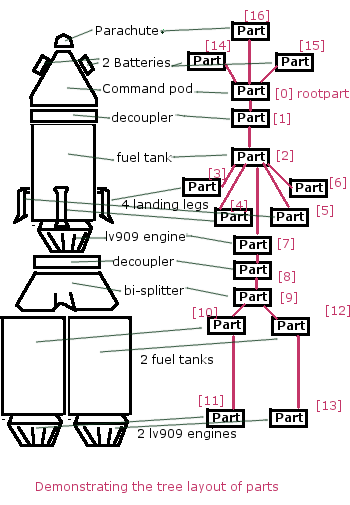
\includegraphics{ship_parts_tree.png}
\end{flushright}\end{figure}


\subsubsection{Accessing the parts list as a tree}
\label{general/parts_and_partmodules:accessing-the-parts-list-as-a-tree}
Starting from the root part, Vessel:ROOTPART (SHIP:ROOTPART, TARGET:ROOTPART, or Vessel(``some ship name''):ROOTPART). You can get all its children parts with the Part:CHILDREN suffix. Given any Part, you can access its Parent part with Part:PARENT, and detect if it doesn't have a parent with Part:HASPARENT. By walking this tree you can see how the parts are connected together.

The diagram here shows an example of a small vessel and how it might get represented as a tree of parts in KSP.


\subsubsection{Accessing the parts list as a list}
\label{general/parts_and_partmodules:accessing-the-parts-list-as-a-list}
You can get a list of all the parts on a vessel using the suffix :PARTS, or by using the LIST PARTS IN command. When you do this, the resulting list is a ``flattening'' of the tree of parts, created by use of a depth-first search starting from the root part. In the diagram shown here, the red numbers indicate one possible way the parts might be represented in LIST indeces if you used SHIP:PARTS on such a vessel. Note there is no guarantee it would look exactly like this, as it depends on exactly what order the parts were attached in the VAB.


\subsubsection{Shortcuts to smaller lists of parts}
\label{general/parts_and_partmodules:shortcuts-to-smaller-lists-of-parts}
If you know some of the properties of the parts you're interested in, you can ask kOS to give you a shorter list of parts that just includes those parts, using the following suffixes:

Return a List of just the parts who's name is ``someNameHere'':

\begin{Verbatim}[commandchars=\\\{\}]
\PYG{n}{SET} \PYG{n}{ves} \PYG{n}{TO} \PYG{n}{SHIP}\PYG{p}{.} \PYG{c+c1}{// or Target or Vessel(\PYGZdq{}ship name\PYGZdq{}).}
\PYG{n}{SET} \PYG{n}{PLIST} \PYG{n}{TO} \PYG{n+nl}{ves}\PYG{p}{:}\PYG{n}{PARTSNAMED}\PYG{p}{(}\PYG{l+s}{\PYGZdq{}}\PYG{l+s}{someNameHere}\PYG{l+s}{\PYGZdq{}}\PYG{p}{)}\PYG{p}{.}
\end{Verbatim}

Return a List of just the parts that have had some sort of activity attached to action group 1:

\begin{Verbatim}[commandchars=\\\{\}]
\PYG{n}{SET} \PYG{n}{ves} \PYG{n}{TO} \PYG{n}{SHIP}\PYG{p}{.} \PYG{c+c1}{// or Target or Vessel(\PYGZdq{}ship name\PYGZdq{}).}
\PYG{n}{SET} \PYG{n}{PLIST} \PYG{n}{TO} \PYG{n+nl}{ves}\PYG{p}{:}\PYG{n}{PARTSINGROUP}\PYG{p}{(}\PYG{n}{AG1}\PYG{p}{)}\PYG{p}{.}
\end{Verbatim}


\subsection{PartModules and the right-click menu:}
\label{general/parts_and_partmodules:partmodules-and-the-right-click-menu}
Each Part, in turn has a list of what are called PartModules on it. A PartModule is a collection of variables and executable program hooks that gives the part some of its behaviors and properties. Without a PartModule, a part is really nothing more than a passive bit of structure that has nothing more than a shape, a look, and a strength to it. Some of the parts in the ``structure'' tab of the parts bin, like pure I-beams and girders, are like this - they have no PartModules on them. But all of the \emph{interesting} parts you might want to do something with will have a PartModule on them. Through PartModules, **kOS will now allow you to manipulate or query anything that any KSP programmer, stock or mod, has added to the rightclick menu**, or action group actions, for a part.


\subsubsection{PartModules, Stock vs Mods:}
\label{general/parts_and_partmodules:partmodules-stock-vs-mods}
It should be noted that even if you play an entirely stock installation of KSP (well, stock other than for kOS, obviously, otherwise you wouldn't be reading this), you will still have PartModules on your Parts. Some people have muddied the terminology difference between ``Mod'' meaning ``modification'' and ``Mod'' meaning ``module''. It should be made absolutely clear that PartModules are a feature of stock KSP, and BOTH stock KSP parts and Modded KSP Parts use them. Even if all you want to do is affect the stock behavior of stock parts in a completely unmodded way, you'll still want to know about PartModules in order to do so.


\subsubsection{PartModules and ModuleManager-like behavior:}
\label{general/parts_and_partmodules:partmodules-and-modulemanager-like-behavior}
Some Mods (meaning ``modifications'' here) operate by adding a new PartModule to every single part in the game. One example of such a mod is the Deadly Reentry mod. In order to track how fragile each part is and how well it withstands re-entry heat, the Deadly Re-entry mod adds a small module to each part in the game, even the stock parts that would normally have no mods at all on them.

Other Mods allow the user to add PartModule's to any part they feel like, through the use of the ModuleManager mod.

Because of these, it's impossible in this explanatory document to make blanket statements about which PartModules will exist on which Parts. Everything that is said here needs to be taken with a grain of salt, as depending on the mods you've installed on your game, you may find PartModules on your parts that are not normally on those parts for most other players.


\subsection{What a PartModule means to a kOS script}
\label{general/parts_and_partmodules:what-a-partmodule-means-to-a-kos-script}
There are 3 ways that a kOS script may interface with a PartModule.

TODO - TAKE SOME SCREENSHOTS TO PUT ALONGSIDE THIS TEXT, SHOWING EXAMPLES OF THESE THINGS IN THE USER INTERFACE. WE NEED A SCREENSHOT THAT SHOWS BOTH A KSPFIELD AND A KSPEVENT IN A PART'S RMB CONTEXT MENU, A SCREENSHOT THAT SHOWS FIELDS COMING FROM MULTIPLE PARTMODULES, AND A SCREENSHOT SHOWING THE KSPACTIONS IN THE VAB ACTION EDITOR.


\subsubsection{KSPFields}
\label{general/parts_and_partmodules:kspfields}
A KSPField is a single variable that a PartModule attaches to a part. Some of the KSPFields are also displayed in the RMB context menu of a part. It has a current value, and if the field has had a ``tweakable'' GUI interface attached to it, then it's also a settable field by the user manipulating the field in the context menu. In kOS, you can only access those KSPFields that are currently visible on the RMB context menu. We, the developers of kOS, instituted this rule out of respect for the developers of other mods and the stock KSP game. If they didn't allow the user to see or manipulate the variable directly in the GUI, then we shouldn't allow it to be manipulated or seen by a kOS script either.

KSPFields are read or manipulated by the following suffixes of PartModule
\begin{itemize}
\item {} 
:GETFIELD(``name of field'').

\item {} 
:SETFIELD(``name of field'', new\_value\_for\_field).

\end{itemize}

Note, that these are suffixes of the partmodule and NOT suffixes of the Part itself. This is because two different PartModule's on the same Part might have used the same field name as each other, and it's important to keep them separate.


\subsubsection{KSPEvents}
\label{general/parts_and_partmodules:kspevents}
A KSPEvent, just like a KSPField, is a thing that a PartModule can put on the RMB context menu for a part. The difference is that a KSPEvent does not actually HAVE a value. It's not a variable. Rather it's just a button with a label next to it. When you press the button, it causes some sort of software inside the PartModule to run. An example of this is the ``undock node'' button you see on many of the docking ports.

\textbf{Difference between a KSPEvent and a boolean KSPField}: If you see a label next to a button in the RMB context menu, it might be a KSPEvent, OR it might be a boolean KSPField variable which is editable with a tweakable GUI. They look exactly the same in the user interface. To tell the difference, you need to look at what happens when you click the button. If clicking the button causes the button to depress inward and stay pressed in until you click it again, then this is a boolean value KSPField. If clicking the button pops the button in and then it pops out again right away, then this is a KSPEvent instead.

KSPEvents are manipulated by the following suffix of PartModule
\begin{itemize}
\item {} 
:DOEVENT(``name of event'').

\end{itemize}

This causes the event to execute once.


\subsubsection{KSPActions:}
\label{general/parts_and_partmodules:kspactions}
A KSPAction is a bit different from a KSPField or KSPEvent. A KSPAction is like a KSPEvent in that it causes some software inside the PartModule to be run. But it doesn't work via the RMB context menu for the part. Instead KSPAction's are those things you see being made avaiable to you as options you can assign into an Action Group in the VAB or SPH. When you have the action group editor tab enabled in the VAB or SPH, and then click on a part, that part asks all of its PartModules if they have any KSPActions they'd like to provide access to, and gathers all those answers and lists them in the user interface for you to select from and assign to the action group.

kOS now allows you to access any of those actions without necessarily having had to assign them to any action groups if you didn't want to.

KSPActions are manipulated by the following suffix of PartModule
\begin{itemize}
\item {} 
:DOACTION(``name of action'', new\_boolan\_value).

\end{itemize}

The name of the action is the name you see in the action group editor interface, and the new boolean value is either True or False. Unlike KSPEvents, a KSPAction has two states, true and false. When you toggle the brakes, for example, they go from on to off, or from off to on. When you call :DOACTION, you are specifying if the KSPAction should behave as if you have just toggled the group on, or just toggled the group off. But instead of actually toggling an action group - you are just telling the single PartModule on a single Part to perform the same behavior it would have performed had that action been assigned to an action group. You don't \emph{actually} have to assign the action to an action group for this to work.


\subsection{Exploring what's there to find Field/Event/Action Names:}
\label{general/parts_and_partmodules:exploring-what-s-there-to-find-field-event-action-names}
Okay, so you understand all that, but you're still thinking ``but how do I KNOW what the names of part modules are, or what the names of the fields on them are? I didn't write all that C\# source code for all the modules.''

There are some additional suffixes that are designed to help you explore what's available so you can learn the answers to these questions. Also, some of the questions can be answered by other means:


\subsubsection{What PartModules are there on a part?}
\label{general/parts_and_partmodules:what-partmodules-are-there-on-a-part}
To answer this question you can do one of two things:

A: \textbf{Use the part.cfg file} All parts in KSP come with a part.cfg file defining them, both for modded parts and stock parts. If you look at this file, it will contain sections looking something like this:

\begin{Verbatim}[commandchars=\\\{\}]
\PYG{c+c1}{// Example snippet from a Part.cfg file:}
\PYG{n}{MODULE}
\PYG{p}{\PYGZob{}}
    \PYG{n}{name} \PYG{o}{=} \PYG{n}{ModuleCommand}
\end{Verbatim}

That would tell you that this part has a PartModule on it called ModuleCommand. there can be multiple such modules per part. But it doesn't let you know about PartModules that get added afterward during runtime, by such things as the ModuleManager mod.

B: \textbf{Use the :MODULES suffix of Part:} If you have a handle on any part in kOS, you can print out the value of :MODULES and it will tell you the string names of all the modules on the part. For example:

\begin{Verbatim}[commandchars=\\\{\}]
\PYG{n}{FOR} \PYG{n}{P} \PYG{n}{IN} \PYG{n+nl}{SHIP}\PYG{p}{:}\PYG{n}{PARTS} \PYG{p}{\PYGZob{}}
  \PYG{n}{LOG} \PYG{p}{(}\PYG{l+s}{\PYGZdq{}}\PYG{l+s}{MODULES FOR PART NAMED }\PYG{l+s}{\PYGZdq{}} \PYG{o}{+} \PYG{n+nl}{P}\PYG{p}{:}\PYG{n}{NAME}\PYG{p}{)} \PYG{n}{TO} \PYG{n}{MODLIST}\PYG{p}{.}
  \PYG{n}{LOG} \PYG{n+nl}{P}\PYG{p}{:}\PYG{n}{MODULES} \PYG{n}{TO} \PYG{n}{MODLIST}\PYG{p}{.}
\PYG{p}{\PYGZcb{}}\PYG{p}{.}
\end{Verbatim}

Do that, and the file MODLIST should now contain a verbose dump of all the module names of all the parts on your ship. You can get any of the modules now by using Part:GETMODULE(``module name'').


\subsubsection{What are the names of the stuff that a PartModule can do?}
\label{general/parts_and_partmodules:what-are-the-names-of-the-stuff-that-a-partmodule-can-do}
These three suffixes tell you everything a part module can do:

\begin{Verbatim}[commandchars=\\\{\}]
\PYG{n}{SET} \PYG{n}{MOD} \PYG{n}{TO} \PYG{n+nl}{P}\PYG{p}{:}\PYG{n}{GETMODULE}\PYG{p}{(}\PYG{l+s}{\PYGZdq{}}\PYG{l+s}{some name here}\PYG{l+s}{\PYGZdq{}}\PYG{p}{)}\PYG{p}{.}
\PYG{n}{LOG} \PYG{p}{(}\PYG{l+s}{\PYGZdq{}}\PYG{l+s}{These are all the things that I can currently USE GETFIELD AND SETFIELD ON IN }\PYG{l+s}{\PYGZdq{}} \PYG{o}{+} \PYG{n+nl}{MOD}\PYG{p}{:}\PYG{n}{NAME} \PYG{o}{+} \PYG{l+s}{\PYGZdq{}}\PYG{l+s}{:}\PYG{l+s}{\PYGZdq{}}\PYG{p}{)} \PYG{n}{TO} \PYG{n}{NAMELIST}\PYG{p}{.}
\PYG{n}{LOG} \PYG{n+nl}{MOD}\PYG{p}{:}\PYG{n}{ALLFIELDS} \PYG{n}{TO} \PYG{n}{NAMELIST}\PYG{p}{.}
\PYG{n}{LOG} \PYG{p}{(}\PYG{l+s}{\PYGZdq{}}\PYG{l+s}{These are all the things that I can currently USE DOEVENT ON IN }\PYG{l+s}{\PYGZdq{}} \PYG{o}{+}  \PYG{n+nl}{MOD}\PYG{p}{:}\PYG{n}{NAME} \PYG{o}{+} \PYG{l+s}{\PYGZdq{}}\PYG{l+s}{:}\PYG{l+s}{\PYGZdq{}}\PYG{p}{)} \PYG{n}{TO} \PYG{n}{NAMELIST}\PYG{p}{.}
\PYG{n}{LOG} \PYG{n+nl}{MOD}\PYG{p}{:}\PYG{n}{ALLEVENTS} \PYG{n}{TO} \PYG{n}{NAMELIST}\PYG{p}{.}
\PYG{n}{LOG} \PYG{p}{(}\PYG{l+s}{\PYGZdq{}}\PYG{l+s}{These are all the things that I can currently USE DOACTION ON IN }\PYG{l+s}{\PYGZdq{}} \PYG{o}{+}  \PYG{n+nl}{MOD}\PYG{p}{:}\PYG{n}{NAME} \PYG{o}{+} \PYG{l+s}{\PYGZdq{}}\PYG{l+s}{:}\PYG{l+s}{\PYGZdq{}}\PYG{p}{)} \PYG{n}{TO} \PYG{n}{NAMELIST}\PYG{p}{.}
\PYG{n}{LOG} \PYG{n+nl}{MOD}\PYG{p}{:}\PYG{n}{ALLACTIONS} \PYG{n}{TO} \PYG{n}{NAMELIST}\PYG{p}{.}
\end{Verbatim}

After that, the file NAMELIST would contain a dump of all the fields on this part module that you can use.


\subsubsection{BE WARNED! Names are able to dynamically change!}
\label{general/parts_and_partmodules:be-warned-names-are-able-to-dynamically-change}
Some PartModules are written to change the name of a field when something happens in the game. For example, you might find that after you've done this:

\begin{Verbatim}[commandchars=\\\{\}]
\PYG{n+nl}{SomeModule}\PYG{p}{:}\PYG{n}{DOEVENT}\PYG{p}{(}\PYG{l+s}{\PYGZdq{}}\PYG{l+s}{Activate}\PYG{l+s}{\PYGZdq{}}\PYG{p}{)}\PYG{p}{.}
\end{Verbatim}

That this doesn't work anymore after that, and the ``Activate'' event now causes an error.

And the reason is that the PartModule chose to change the label on the event. It changed to the word ``Deactivate'' now. kOS can no longer trigger an event called ``Activate'' because that's no longer its name.

Be on the lookout for cases like this. Experiment with how the context menu is being manipulated and keep in mind that the list of strings you got the last time you exectued :ALLFIELDS a few minutes ago might not be the same list you'd get if you ran it now, because the PartModule has changed what is being shown on the menu.


\section{Career Limits}
\label{general/career_limits:career-limits}\label{general/career_limits::doc}\label{general/career_limits:id1}
The theme of KSP 0.90 is that some features of your space program don't work until after you've made some upgrades.
kOS now supports enforcing these checks, as described below.
\setbox0\vbox{
\begin{minipage}{0.95\linewidth}
\begin{itemize}
\item {} 
\phantomsection\label{general/career_limits:id3}{\hyperref[general/career_limits:the-rules-being-enforced]{\emph{The rules being enforced}}}

\item {} 
\phantomsection\label{general/career_limits:id4}{\hyperref[general/career_limits:structure]{\emph{Structure}}}

\end{itemize}
\end{minipage}}
\begin{center}\setlength{\fboxsep}{5pt}\shadowbox{\box0}\end{center}

\begin{notice}{warning}{Warning:}\end{notice}


\subsection{The rules being enforced}
\label{general/career_limits:the-rules-being-enforced}
These are rules inherited from the stock KSP game that kOS is simply adhering to:
\begin{itemize}
\item {} 
If your tracking center is not upgraded far enough, then you cannot see
future orbit patches.

\item {} 
If your mission control center AND tracking center are not upgraded enough,
then you cannot add manuever nodes.

\end{itemize}

The following are rules invented by kOS that are thematically very similar to stock KSP, intended to be as close to the meaning of the stock game's rules as possible:
\begin{itemize}
\item {} 
In order to be allowed to execute the {\hyperref[structures/vessels/partmodule:structure:PARTMODULE]{\emph{\code{PartModule}}}} :DOACTION method, either
your VAB or your SPH must be upgraded to the point where it will allow access to
custom action groups.  This is because otherwise the :DOACTION method would be a
backdoor ``cheat'' past the restricted access to the action group feaures of various
PartModules that the game is meant to have.

\item {} 
In order to be allowed to add a \code{nametag} to parts inside the editor so they get
saved to the craft file, you must have upgraded your current editor building (VAB or
SPH, depending) to the point where it allows at least stock action groups.  This is
because name tags are a sort of semi-advanced feature.

\end{itemize}

You can see some of these settings by reading the values of the Career() global object,
for example:
\begin{description}
\item[{::}] \leavevmode
print Career():PATCHLIMIT.
print Career():CANDOACTIONS.

\end{description}


\subsection{Structure}
\label{general/career_limits:structure}\index{Career {[}struct{]}}

\begin{fulllineitems}
\phantomsection\label{general/career_limits:structure:CAREER}\pysigline{\strong{structure }\bfcode{Career}}~

\begin{threeparttable}
\capstart\caption{Members}
\label{general/career_limits:id2}
\begin{tabulary}{\linewidth}{|L|L|L|L|}
\hline
\textsf{\relax 
Suffix
} & \textsf{\relax 
Type
} & \textsf{\relax 
Get
} & \textsf{\relax 
Set
}\\
\hline
{\hyperref[general/career_limits:attribute:CAREER:CANTRACKOBJECTS]{\emph{\code{CANTRACKOBJECTS}}}}
 & 
boolean
 & 
yes
 & 
no
\\
\hline
{\hyperref[general/career_limits:attribute:CAREER:PATCHLIMIT]{\emph{\code{PATCHLIMIT}}}}
 & 
number
 & 
yes
 & 
no
\\
\hline
{\hyperref[general/career_limits:attribute:CAREER:CANMAKENODES]{\emph{\code{CANMAKENODES}}}}
 & 
boolean
 & 
yes
 & 
no
\\
\hline
{\hyperref[general/career_limits:attribute:CAREER:CANDOACTIONS]{\emph{\code{CANDOACTIONS}}}}
 & 
boolean
 & 
yes
 & 
no
\\
\hline\end{tabulary}

\end{threeparttable}


\end{fulllineitems}

\index{Career:CANTRACKOBJECTS}

\begin{fulllineitems}
\phantomsection\label{general/career_limits:attribute:CAREER:CANTRACKOBJECTS}\pysigline{Career:\bfcode{CANTRACKOBJECTS}}~\begin{quote}\begin{description}
\item[{Type}] \leavevmode
boolean

\item[{Access}] \leavevmode
Get

\end{description}\end{quote}

If your tracking center allows the tracking of unnamed objects (asteroids, mainly) then this will return true.

\end{fulllineitems}

\index{Career:PATCHLIMIT}

\begin{fulllineitems}
\phantomsection\label{general/career_limits:attribute:CAREER:PATCHLIMIT}\pysigline{Career:\bfcode{PATCHLIMIT}}~\begin{quote}\begin{description}
\item[{Type}] \leavevmode
number

\item[{Access}] \leavevmode
Get

\end{description}\end{quote}

If your tracking center allows some patched conics predictions, then this number will be greater than zero.
The number represents how many patches beyond the current one that you are allowed to see.  It influences
attempts to call SHIP:PATCHES and SHIP:OBT:NEXTPATCH.

\end{fulllineitems}

\index{Career:CANMAKENODES}

\begin{fulllineitems}
\phantomsection\label{general/career_limits:attribute:CAREER:CANMAKENODES}\pysigline{Career:\bfcode{CANMAKENODES}}~\begin{quote}\begin{description}
\item[{Type}] \leavevmode
boolean

\item[{Access}] \leavevmode
Get

\end{description}\end{quote}

If your tracking center and mission control buildings are both upgraded enough, then the game allows
you to make manuever nodes (which the game calls ``flight planning'').  This will return true if you
can make maneuver nodes.

\end{fulllineitems}

\index{Career:CANDOACTIONS}

\begin{fulllineitems}
\phantomsection\label{general/career_limits:attribute:CAREER:CANDOACTIONS}\pysigline{Career:\bfcode{CANDOACTIONS}}~\begin{quote}\begin{description}
\item[{Type}] \leavevmode
boolean

\item[{Access}] \leavevmode
Get

\end{description}\end{quote}

If your VAB or SPH are upgraded enough to allow custom action groups, then you will also be allowed
to execute the :DOACTION method of PartModules.  Otherwise you can't.  This will return a boolean
letting you know if the condition has been met.

\end{fulllineitems}



\chapter{The \textbf{KerboScript} Language}
\label{language::doc}\label{language:language}\label{language:the-kerboscript-language}

\section{General Features of the \textbf{KerboScript} Language}
\label{language/features:general-features-of-the-kerboscript-language}\label{language/features::doc}\label{language/features:features}\setbox0\vbox{
\begin{minipage}{0.95\linewidth}
\begin{itemize}
\item {} 
\phantomsection\label{language/features:id2}{\hyperref[language/features:case-insensitivity]{\emph{Case Insensitivity}}}

\item {} 
\phantomsection\label{language/features:id3}{\hyperref[language/features:expressions]{\emph{Expressions}}}
\begin{itemize}
\item {} 
\phantomsection\label{language/features:id4}{\hyperref[language/features:numbers]{\emph{1. Numbers}}}

\item {} 
\phantomsection\label{language/features:id5}{\hyperref[language/features:strings]{\emph{2. Strings}}}

\item {} 
\phantomsection\label{language/features:id6}{\hyperref[language/features:structures]{\emph{3. Structures}}}

\item {} 
\phantomsection\label{language/features:id7}{\hyperref[language/features:structure-methods]{\emph{4. Structure Methods}}}

\end{itemize}

\item {} 
\phantomsection\label{language/features:id8}{\hyperref[language/features:short-curcuiting-booleans]{\emph{Short-curcuiting booleans}}}

\item {} 
\phantomsection\label{language/features:id9}{\hyperref[language/features:late-typing]{\emph{Late Typing}}}

\item {} 
\phantomsection\label{language/features:id10}{\hyperref[language/features:lazy-globals-variable-declarations-optional]{\emph{Lazy Globals (variable declarations optional)}}}

\item {} 
\phantomsection\label{language/features:id11}{\hyperref[language/features:user-functions]{\emph{User Functions}}}

\item {} 
\phantomsection\label{language/features:id12}{\hyperref[language/features:language-structures]{\emph{Structures}}}

\end{itemize}
\end{minipage}}
\begin{center}\setlength{\fboxsep}{5pt}\shadowbox{\box0}\end{center}


\subsection{Case Insensitivity}
\label{language/features:case-insensitivity}
Everything in \textbf{KerboScript} is case-insensitive, including your own variable names and filenames. The only exception is when you perform a string comparison, (\code{"Hello"="HELLO"} will return false.)

Most of the examples here will show the syntax in all-uppercase to help make it stand out from the explanatory text.


\subsection{Expressions}
\label{language/features:expressions}
KerboScript uses an expression evaluation system that allows you to perform math operations on variables. Some variables are defined by you. Others are defined by the system. There are four basic types:


\subsubsection{1. Numbers}
\label{language/features:numbers}
You can use mathematical operations on numbers, like this:

\begin{Verbatim}[commandchars=\\\{\}]
\PYG{n}{SET} \PYG{n}{X} \PYG{n}{TO} \PYG{l+m+mi}{4} \PYG{o}{+} \PYG{l+m+mf}{2.5}\PYG{p}{.}
\PYG{n}{PRINT} \PYG{n}{X}\PYG{p}{.}             \PYG{c+c1}{// Outputs 6.5}
\end{Verbatim}

The system follows the order of operations, but currently the implementation is imperfect. For example, multiplication will always be performed before division, regardless of the order they come in. This will be fixed in a future release.


\subsubsection{2. Strings}
\label{language/features:strings}
Strings are pieces of text that are generally meant to be printed to the screen. For example:

\begin{Verbatim}[commandchars=\\\{\}]
\PYG{n}{PRINT} \PYG{l+s}{\PYGZdq{}}\PYG{l+s}{Hello World!}\PYG{l+s}{\PYGZdq{}}\PYG{p}{.}
\end{Verbatim}

To concatenate strings, you can use the + operator. This works with mixtures of numbers and strings as well:

\begin{Verbatim}[commandchars=\\\{\}]
\PYG{n}{PRINT} \PYG{l+s}{\PYGZdq{}}\PYG{l+s}{4 plus 3 is: }\PYG{l+s}{\PYGZdq{}} \PYG{o}{+} \PYG{p}{(}\PYG{l+m+mi}{4}\PYG{o}{+}\PYG{l+m+mi}{3}\PYG{p}{)}\PYG{p}{.}
\end{Verbatim}


\subsubsection{3. Structures}
\label{language/features:structures}\label{language/features:features-structures}
Structures are variables that contain more than one piece of information. For example, a Vector has an X, a Y, and a Z component. Structures can be used with SET.. TO just like any other variable. To access the sub-elements of a structure, you use the colon operator ('':''). Here are some examples:

\begin{Verbatim}[commandchars=\\\{\}]
\PYG{n}{PRINT} \PYG{l+s}{\PYGZdq{}}\PYG{l+s}{The Mun\PYGZsq{}s periapsis altitude is: }\PYG{l+s}{\PYGZdq{}} \PYG{o}{+} \PYG{n+nl}{MUN}\PYG{p}{:}\PYG{n}{PERIAPSIS}\PYG{p}{.}
\PYG{n}{PRINT} \PYG{l+s}{\PYGZdq{}}\PYG{l+s}{The ship\PYGZsq{}s surface velocity is: }\PYG{l+s}{\PYGZdq{}} \PYG{o}{+} \PYG{n+nl}{SHIP}\PYG{p}{:}\PYG{n+nl}{VELOCITY}\PYG{p}{:}\PYG{n}{SURFACE}\PYG{p}{.}
\end{Verbatim}

Many structures also let you set a specific component of them, for example:

\begin{Verbatim}[commandchars=\\\{\}]
\PYG{n}{SET} \PYG{n}{VEC} \PYG{n}{TO} \PYG{n}{V}\PYG{p}{(}\PYG{l+m+mi}{10}\PYG{p}{,}\PYG{l+m+mi}{10}\PYG{p}{,}\PYG{l+m+mi}{10}\PYG{p}{)}\PYG{p}{.}  \PYG{c+c1}{// A vector with x,y,z components}
                         \PYG{c+c1}{// all set to 10.}
\PYG{n}{SET} \PYG{n+nl}{VEC}\PYG{p}{:}\PYG{n}{X} \PYG{n}{to} \PYG{n+nl}{VEC}\PYG{p}{:}\PYG{n}{X} \PYG{o}{*} \PYG{l+m+mf}{4.}  \PYG{c+c1}{// multiply just the X part of VEC by 4.}
\PYG{n}{PRINT} \PYG{n}{VEC}\PYG{p}{.}               \PYG{c+c1}{// Results in V(40,10,10).}
\end{Verbatim}


\subsubsection{4. Structure Methods}
\label{language/features:features-methods}\label{language/features:structure-methods}
Structures also often contain methods. A method is a suffix of a structure that actually performs an activity when you mention it, and can sometimes take parameters. The following are examples of calling methods of a structure:

\begin{Verbatim}[commandchars=\\\{\}]
\PYG{n}{SET} \PYG{n}{PLIST} \PYG{n}{TO} \PYG{n+nl}{SHIP}\PYG{p}{:}\PYG{n}{PARTSDUBBED}\PYG{p}{(}\PYG{l+s}{\PYGZdq{}}\PYG{l+s}{my engines}\PYG{l+s}{\PYGZdq{}}\PYG{p}{)}\PYG{p}{.} \PYG{c+c1}{// calling a suffix}
                                             \PYG{c+c1}{// method with one}
                                             \PYG{c+c1}{// argument that}
                                             \PYG{c+c1}{// returns a list.}
\PYG{n+nl}{PLIST}\PYG{p}{:}\PYG{n}{REMOVE}\PYG{p}{(}\PYG{l+m+mi}{0}\PYG{p}{)}\PYG{p}{.} \PYG{c+c1}{// calling a suffix method with one argument that}
                 \PYG{c+c1}{// doesn\PYGZsq{}t return anything.}
\PYG{n}{PRINT} \PYG{n+nl}{PLIST}\PYG{p}{:}\PYG{n}{SUBLIST}\PYG{p}{(}\PYG{l+m+mi}{0}\PYG{p}{,}\PYG{l+m+mi}{4}\PYG{p}{)}\PYG{p}{.} \PYG{c+c1}{// calling a suffix method with 2}
                          \PYG{c+c1}{// arguments that returns a list.}
\end{Verbatim}

\begin{notice}{note}{Note:}
\DUspan{versionmodified}{New in version 0.15: }Methods now perform the activity when the interpreter comes up to it. Prior to this version, execution was sometimes delayed until some later time depending on the trigger setup or flow-control.
\end{notice}

For more information, see the {\hyperref[language/features:language-structures]{\emph{\DUspan{}{Structures Section}}}}. A full list of structure types can be found on the {\hyperref[structures:structures]{\emph{\DUspan{}{Structures}}}} page. For a more detailed breakdown of the language, see the {\hyperref[language/syntax:syntax]{\emph{\DUspan{}{Language Syntax Constructs}}}} page.


\subsection{Short-curcuiting booleans}
\label{language/features:short-circuit}\label{language/features:short-curcuiting-booleans}
Further reading: \href{https://en.wikipedia.org/wiki/Short-circuit\_evaluation}{https://en.wikipedia.org/wiki/Short-circuit\_evaluation}

When performing any boolean operation involving the use of the AND or the OR
operator, kerboscript will short-circuit the boolean check.  What this means
is that if it gets to a point in the expression where it already knows the
result is a forgone conclusion, it doesn't bother calculating the rest of
the expression and just quits there.

Example:

\begin{Verbatim}[commandchars=\\\{\}]
\PYG{n}{set} \PYG{n}{x} \PYG{n}{to} \PYG{n+nb}{true}\PYG{p}{.}
\PYG{k}{if} \PYG{n}{x} \PYG{n}{or} \PYG{n}{y}\PYG{o}{+}\PYG{l+m+mi}{2} \PYG{o}{\PYGZgt{}} \PYG{l+m+mi}{10} \PYG{p}{\PYGZob{}}
    \PYG{n}{print} \PYG{l+s}{\PYGZdq{}}\PYG{l+s}{yes}\PYG{l+s}{\PYGZdq{}}\PYG{p}{.}
\PYG{p}{\PYGZcb{}} \PYG{k}{else} \PYG{p}{\PYGZob{}}
    \PYG{n}{print} \PYG{l+s}{\PYGZdq{}}\PYG{l+s}{no}\PYG{l+s}{\PYGZdq{}}\PYG{p}{.}
\PYG{p}{\PYGZcb{}}\PYG{p}{.}
\end{Verbatim}

In this case, the fact that x is true means that when evaluating
the boolean expression \code{x or y+2 \textgreater{} 10} it never even bothers trying
to add y and 2 to find out if it's greater than 10.  It already knew
as soon as it got to the \code{x or whatever} that given that x is true,
the \emph{whatever} doesn't matter one bit.  Once one side of an OR is true,
the other side can either be true or false and it won't change the fact
that the whole expression will be true anyway.

A similar short circuiting happens with AND.  Once the left side of the
AND operator is false, then the entire AND expression is guaranteed
to be false regardless of what's on the right side, so kerboscript
doesn't bother calculating the righthand side once the lefthand side is false.

Read the link above for implications of why this matters in programming.


\subsection{Late Typing}
\label{language/features:late-typing}
Kerboscript is a language in which there is only one type of variable
and it just generically holds any sort of object of any kind.  If
you attempt to assign, for example, a string into a variable that is
currently holding an integer, this does not generate an error.  It
simply causes the variable to change its type and no longer be an
integer, becoming a string now.

In other words, the type of a variable changes dynamically at
runtime depending on what you assign into it.


\subsection{Lazy Globals (variable declarations optional)}
\label{language/features:lazy-globals-variable-declarations-optional}
Kerboscript is a language in which variables need not be declared ahead
of time.  If you simply set a variable to a value, that just ``magically''
makes the variable exist if it didn't already.  When you do this,
the variable will necessarily be \emph{global} in scope.  kerboscript refers
to these variables created implicitly this way as ``lazy globals''.
It's a system designed to make kerboscript easy to use for people new to
programming.

But if you are an experienced programmer you might not like this
behavior, and there are good arguments for why you might want to
disable it.  If you wish to do so, a syntax exists to do so called
:ref:\code{NOLAZYGLOBAL}.


\subsection{User Functions}
\label{language/features:user-functions}\label{language/features:feature-functions}
\begin{notice}{note}{Note:}
\DUspan{versionmodified}{New in version 0.17: }This feature did not exist in prior versions of kerboscript.
\end{notice}

Kerboscript supports user functions which you can write yourself
and call from your own scripts.  \emph{These are not} {\hyperref[language/features:features-methods]{\emph{\DUspan{}{structure
methods}}}} \emph{(which as of this writing are a feature which
only works for the built-in kOS types, and are not yet supported
by the kerboscript language for user functions you write yourself).}

Example:

\begin{Verbatim}[commandchars=\\\{\}]
\PYG{n}{DECLARE} \PYG{n}{FUNCTION} \PYG{n}{DEGREES\PYGZus{}TO\PYGZus{}RADIANS} \PYG{p}{\PYGZob{}}
  \PYG{n}{DECLARE} \PYG{n}{PARAMETER} \PYG{n}{DEG}\PYG{p}{.}

  \PYG{n}{RETURN} \PYG{n}{CONSTANT}\PYG{p}{(}\PYG{p}{)}\PYG{o}{:}\PYG{n}{PI} \PYG{o}{*} \PYG{n}{DEG}\PYG{o}{/}\PYG{l+m+mf}{180.}
\PYG{p}{\PYGZcb{}}\PYG{p}{.}

\PYG{n}{SET} \PYG{n}{ALPHA} \PYG{n}{TO} \PYG{l+m+mf}{45.}
\PYG{n}{PRINT} \PYG{n}{ALPHA} \PYG{o}{+} \PYG{l+s}{\PYGZdq{}}\PYG{l+s}{ degrees is }\PYG{l+s}{\PYGZdq{}} \PYG{o}{+} \PYG{n}{DEGREES\PYGZus{}TO\PYGZus{}RADIANS}\PYG{p}{(}\PYG{n}{ALPHA}\PYG{p}{)} \PYG{o}{+} \PYG{l+s}{\PYGZdq{}}\PYG{l+s}{ radians.}\PYG{l+s}{\PYGZdq{}}\PYG{p}{.}
\end{Verbatim}

For a more detailed description of how to declare your own user functions,
see the {\hyperref[language/syntax:syntax-functions]{\emph{\DUspan{}{Language Syntax Constructs, User Functions}}}}
section.


\subsection{Structures}
\label{language/features:language-structures}\label{language/features:id1}
Structures, {\hyperref[language/features:features-structures]{\emph{\DUspan{}{introduced above}}}}, are variable \emph{types} that contain more than one piece of information. All structures contain sub-values or {\hyperref[language/features:features-methods]{\emph{\DUspan{}{methods}}}} that can be accessed with a colon (\code{:}) operator. Multiple structures can be chained together with more than one colon (\code{:}) operator:

\begin{Verbatim}[commandchars=\\\{\}]
\PYG{n}{SET} \PYG{n}{myCraft} \PYG{n}{TO} \PYG{n}{SHIP}\PYG{p}{.}
\PYG{n}{SET} \PYG{n}{myMass} \PYG{n}{TO} \PYG{n+nl}{myCraft}\PYG{p}{:}\PYG{n}{MASS}\PYG{p}{.}
\PYG{n}{SET} \PYG{n}{myVel} \PYG{n}{TO} \PYG{n+nl}{myCraft}\PYG{p}{:}\PYG{n+nl}{VELOCITY}\PYG{p}{:}\PYG{n}{ORBIT}\PYG{p}{.}
\end{Verbatim}

These terms are referred to as ``suffixes''. For example \code{Velocity} is a suffix of \code{Vessel}. It is possible to \textbf{set} some suffixes as well. The second line in the following example sets the \code{ETA} of a \code{NODE} 500 seconds into the future:

\begin{Verbatim}[commandchars=\\\{\}]
\PYG{n}{SET} \PYG{n}{n} \PYG{n}{TO} \PYG{n}{Node}\PYG{p}{(} \PYG{n+nl}{TIME}\PYG{p}{:}\PYG{n}{SECONDS} \PYG{o}{+} \PYG{l+m+mi}{60}\PYG{p}{,} \PYG{l+m+mi}{0}\PYG{p}{,} \PYG{l+m+mi}{10}\PYG{p}{,} \PYG{l+m+mi}{10}\PYG{p}{)}\PYG{p}{.}
\PYG{n}{SET} \PYG{n+nl}{n}\PYG{p}{:}\PYG{n}{ETA} \PYG{n}{to} \PYG{l+m+mf}{500.}
\end{Verbatim}

The full list of available suffixes for each type {\hyperref[structures:structures]{\emph{\DUspan{}{can be found here}}}}.


\section{\textbf{KerboScript} Syntax Specification}
\label{language/syntax::doc}\label{language/syntax:kerboscript-syntax-specification}\label{language/syntax:syntax}
This describes what is and is not a syntax error in the \textbf{KerboScript} programming language. It does not describe what function calls exist or which commands and built-in variables are present. Those are contained in other documents.
\setbox0\vbox{
\begin{minipage}{0.95\linewidth}
\textbf{Contents}

\medskip

\begin{itemize}
\item {} 
\phantomsection\label{language/syntax:id1}{\hyperref[language/syntax:general-rules]{\emph{General Rules}}}

\item {} 
\phantomsection\label{language/syntax:id2}{\hyperref[language/syntax:braces-statement-blocks]{\emph{Braces (statement blocks)}}}

\item {} 
\phantomsection\label{language/syntax:id3}{\hyperref[language/syntax:functions-built-in]{\emph{Functions (built-in)}}}

\item {} 
\phantomsection\label{language/syntax:id4}{\hyperref[language/syntax:suffixes-as-functions-methods]{\emph{Suffixes as Functions (Methods)}}}

\item {} 
\phantomsection\label{language/syntax:id5}{\hyperref[language/syntax:user-functions]{\emph{User Functions}}}

\item {} 
\phantomsection\label{language/syntax:id6}{\hyperref[language/syntax:built-in-special-variable-names]{\emph{Built-In Special Variable Names}}}

\item {} 
\phantomsection\label{language/syntax:id7}{\hyperref[language/syntax:what-does-not-exist-yet]{\emph{What does not exist (yet?)}}}

\end{itemize}
\end{minipage}}
\begin{center}\setlength{\fboxsep}{5pt}\shadowbox{\box0}\end{center}


\subsection{General Rules}
\label{language/syntax:general-rules}
\emph{Whitespace} consisting of consecutive spaces, tabs, and line breaks are all considered identical to each other. Because of this, indentation is up to you. You may indent however you like.

\begin{notice}{note}{Note:}
Statements are ended with a \textbf{period} character (''.'').
\end{notice}

The following are \textbf{reserved command keywords} and special
operator symbols:

\textbf{Arithmetic Operators}:

\begin{Verbatim}[commandchars=\\\{\}]
\PYG{o}{+}  \PYG{o}{\PYGZhy{}}  \PYG{o}{*}  \PYG{o}{/}  \PYG{o}{\PYGZca{}}  \PYG{n}{e}  \PYG{p}{(}  \PYG{p}{)}
\end{Verbatim}

\textbf{Logic Operators}:

\begin{Verbatim}[commandchars=\\\{\}]
\PYG{n}{not}  \PYG{n}{and}  \PYG{n}{or}  \PYG{n+nb}{true}  \PYG{n+nb}{false}  \PYG{o}{\PYGZlt{}}\PYG{o}{\PYGZgt{}}  \PYG{o}{\PYGZgt{}}\PYG{o}{=}  \PYG{o}{\PYGZlt{}}\PYG{o}{=}  \PYG{o}{=}  \PYG{o}{\PYGZgt{}}  \PYG{o}{\PYGZlt{}}
\end{Verbatim}

\textbf{Instructions and keywords}:

\begin{Verbatim}[commandchars=\\\{\}]
\PYG{n}{set}  \PYG{n}{to}  \PYG{k}{if}  \PYG{k}{else} \PYG{n}{from} \PYG{n}{until} \PYG{n}{step} \PYG{k}{do} \PYG{n}{lock}  \PYG{n}{unlock}  \PYG{n}{print}  \PYG{n}{at}  \PYG{n}{on}  \PYG{n}{toggle}
\PYG{n}{wait}  \PYG{n}{when}  \PYG{n}{then}  \PYG{n}{off}  \PYG{n}{stage}  \PYG{n}{clearscreen}  \PYG{n}{add}  \PYG{n}{remove}  \PYG{n}{log}
\PYG{k}{break}  \PYG{n}{preserve}  \PYG{n}{declare}  \PYG{n}{parameter}  \PYG{k}{switch}  \PYG{n}{copy}  \PYG{n}{rename}
\PYG{n}{volume}  \PYG{n}{file}  \PYG{n}{delete}  \PYG{n}{edit}  \PYG{n}{run}  \PYG{n}{compile}  \PYG{n}{list}  \PYG{n}{reboot}  \PYG{n}{shutdown}
\PYG{k}{for}  \PYG{n}{unset}  \PYG{n}{batch}  \PYG{n}{deploy}  \PYG{n}{in}  \PYG{n}{all}
\end{Verbatim}

\textbf{Other symbols}:

\begin{Verbatim}[commandchars=\\\{\}]
\PYG{p}{\PYGZob{}}  \PYG{p}{\PYGZcb{}}  \PYG{p}{[}  \PYG{p}{]}  \PYG{p}{,}  \PYG{o}{:}  \PYG{c+c1}{//}
\end{Verbatim}

\emph{Comments} consist of everything from a ``//'' symbol to the end of the line:

\begin{Verbatim}[commandchars=\\\{\}]
\PYG{n}{set} \PYG{n}{x} \PYG{n}{to} \PYG{l+m+mf}{1.} \PYG{c+c1}{// this is a comment.}
\end{Verbatim}

\textbf{Identifiers}: Identifiers consist of: a string of (letter, digit, or
underscore). The first character must be a letter. The rest may be letters, digits or underscores. \textbf{Identifiers are case-insensitive}. The following are identical identifiers:

\begin{Verbatim}[commandchars=\\\{\}]
\PYG{n}{My\PYGZus{}Variable}  \PYG{n}{my\PYGZus{}varible}  \PYG{n}{MY\PYGZus{}VARAIBLE}
\end{Verbatim}
\begin{description}
\item[{\textbf{case-insensitivity}}] \leavevmode
The same case-insensitivity applies throughout the entire language, with all keywords except when comparing literal strings. The values inside the strings are still case-sensitive, for example, the following will print ``unequal'':

\begin{Verbatim}[commandchars=\\\{\}]
\PYG{k}{if} \PYG{l+s}{\PYGZdq{}}\PYG{l+s}{hello}\PYG{l+s}{\PYGZdq{}} \PYG{o}{=} \PYG{l+s}{\PYGZdq{}}\PYG{l+s}{HELLO}\PYG{l+s}{\PYGZdq{}} \PYG{p}{\PYGZob{}}
    \PYG{n}{print} \PYG{l+s}{\PYGZdq{}}\PYG{l+s}{equal}\PYG{l+s}{\PYGZdq{}}\PYG{p}{.}
\PYG{p}{\PYGZcb{}} \PYG{k}{else} \PYG{p}{\PYGZob{}}
    \PYG{n}{print} \PYG{l+s}{\PYGZdq{}}\PYG{l+s}{unequal}\PYG{l+s}{\PYGZdq{}}\PYG{p}{.}
\PYG{p}{\PYGZcb{}}
\end{Verbatim}

\item[{\textbf{Suffixes}}] \leavevmode
Some variable types are structures that contain sub-portions. The separator between the main variable and the item inside it is a colon character (\code{:}). When this symbol is used, the part on the right-hand side of the colon is called the ``suffix'':

\begin{Verbatim}[commandchars=\\\{\}]
\PYG{n}{list} \PYG{n}{parts} \PYG{n}{in} \PYG{n}{mylist}\PYG{p}{.}
\PYG{n}{print} \PYG{n+nl}{mylist}\PYG{p}{:}\PYG{n}{length}\PYG{p}{.} \PYG{c+c1}{// length is a suffix of mylist}
\end{Verbatim}

\end{description}

Suffixes can be chained together, as in this example:

\begin{Verbatim}[commandchars=\\\{\}]
\PYG{n}{print} \PYG{n+nl}{ship}\PYG{p}{:}\PYG{n+nl}{velocity}\PYG{p}{:}\PYG{n+nl}{orbit}\PYG{p}{:}\PYG{n}{x}\PYG{p}{.}
\end{Verbatim}

In the above example you'd say ``\code{velocity} is a suffix of \code{ship}'', and ``\code{orbit} is a suffix of \code{ship:velocity}'', and ``\code{x} is a suffix of \code{ship:velocity:orbit}''.


\subsection{Braces (statement blocks)}
\label{language/syntax:braces-statement-blocks}
Anywhere you feel like, you may insert braces around a list of statements
to get the language to treat them all as a single statement block.

For example: the IF statement expects one statement as its body, like so:

\begin{Verbatim}[commandchars=\\\{\}]
\PYG{k}{if} \PYG{n}{x} \PYG{o}{=} \PYG{l+m+mi}{1}
  \PYG{n}{print} \PYG{l+s}{\PYGZdq{}}\PYG{l+s}{it\PYGZsq{}s 1}\PYG{l+s}{\PYGZdq{}}\PYG{p}{.}
\end{Verbatim}

But you can put multiple statements there as its body by surrounding them
with braces, like so:

\begin{Verbatim}[commandchars=\\\{\}]
\PYG{k}{if} \PYG{n}{x} \PYG{o}{=} \PYG{l+m+mi}{1} \PYG{p}{\PYGZob{}} \PYG{n}{print} \PYG{l+s}{\PYGZdq{}}\PYG{l+s}{it\PYGZsq{}s 1}\PYG{l+s}{\PYGZdq{}}\PYG{p}{.}  \PYG{n}{print} \PYG{l+s}{\PYGZdq{}}\PYG{l+s}{yippieee.}\PYG{l+s}{\PYGZdq{}}\PYG{p}{.}  \PYG{p}{\PYGZcb{}}
\end{Verbatim}

(Although this is usually preferred to be indented as follows):

\begin{Verbatim}[commandchars=\\\{\}]
\PYG{k}{if} \PYG{n}{x} \PYG{o}{=} \PYG{l+m+mi}{1} \PYG{p}{\PYGZob{}}
  \PYG{n}{print} \PYG{l+s}{\PYGZdq{}}\PYG{l+s}{it\PYGZsq{}s 1}\PYG{l+s}{\PYGZdq{}}\PYG{p}{.}
  \PYG{n}{print} \PYG{l+s}{\PYGZdq{}}\PYG{l+s}{yippieee.}\PYG{l+s}{\PYGZdq{}}\PYG{p}{.}
\PYG{p}{\PYGZcb{}}
\end{Verbatim}

or:

\begin{Verbatim}[commandchars=\\\{\}]
\PYG{k}{if} \PYG{n}{x} \PYG{o}{=} \PYG{l+m+mi}{1}
\PYG{p}{\PYGZob{}}
  \PYG{n}{print} \PYG{l+s}{\PYGZdq{}}\PYG{l+s}{it\PYGZsq{}s 1}\PYG{l+s}{\PYGZdq{}}\PYG{p}{.}
  \PYG{n}{print} \PYG{l+s}{\PYGZdq{}}\PYG{l+s}{yippieee.}\PYG{l+s}{\PYGZdq{}}\PYG{p}{.}
\PYG{p}{\PYGZcb{}}
\end{Verbatim}

Kerboscript does not require proper indentation of the brace sections,
but it is a good idea to make things clear.

You are allowed to just insert braces anywhere you feel like even when the
language does not require it, as shown below:

\begin{Verbatim}[commandchars=\\\{\}]
\PYG{n}{declare} \PYG{n}{x} \PYG{n}{to} \PYG{l+m+mf}{3.}
\PYG{n}{print} \PYG{l+s}{\PYGZdq{}}\PYG{l+s}{x here is }\PYG{l+s}{\PYGZdq{}} \PYG{o}{+} \PYG{n}{x}\PYG{p}{.}
\PYG{p}{\PYGZob{}}
  \PYG{n}{declare} \PYG{n}{x} \PYG{n}{to} \PYG{l+m+mf}{5.}
  \PYG{n}{print} \PYG{l+s}{\PYGZdq{}}\PYG{l+s}{x here is }\PYG{l+s}{\PYGZdq{}} \PYG{o}{+} \PYG{n}{x}\PYG{p}{.}
  \PYG{p}{\PYGZob{}}
    \PYG{n}{declare} \PYG{n}{x} \PYG{n}{to} \PYG{l+m+mf}{7.}
    \PYG{n}{print} \PYG{l+s}{\PYGZdq{}}\PYG{l+s}{x here is }\PYG{l+s}{\PYGZdq{}} \PYG{o}{+} \PYG{n}{x}\PYG{p}{.}
  \PYG{p}{\PYGZcb{}}
\PYG{p}{\PYGZcb{}}
\end{Verbatim}

The usual reason for doing this is to create a
{\hyperref[language/variables:scope]{\emph{\DUspan{}{local scope section}}}} for yourself.
In the above example, there are actually 3 \emph{different}
variables called `x' - each with a different scope.


\subsection{Functions (built-in)}
\label{language/syntax:functions-built-in}
There exist a number of built-in functions you can call using their names. When you do so, you can do it like so:

\begin{Verbatim}[commandchars=\\\{\}]
\PYG{n}{functionName}\PYG{p}{(} \PYG{o}{*}\PYG{n}{arguments} \PYG{n}{with} \PYG{n}{commas} \PYG{n}{between} \PYG{n}{them}\PYG{o}{*} \PYG{p}{)}\PYG{p}{.}
\end{Verbatim}

For example, the \code{ROUND} function takes 2 arguments:

\begin{Verbatim}[commandchars=\\\{\}]
\PYG{n}{print} \PYG{n}{ROUND}\PYG{p}{(}\PYG{l+m+mf}{1230.12312}\PYG{p}{,} \PYG{l+m+mi}{2}\PYG{p}{)}\PYG{p}{.}
\end{Verbatim}

The \code{SIN} function takes 1 argument:

\begin{Verbatim}[commandchars=\\\{\}]
\PYG{n}{print} \PYG{n}{SIN}\PYG{p}{(}\PYG{l+m+mi}{45}\PYG{p}{)}\PYG{p}{.}
\end{Verbatim}

When a function requires zero arguments, it is legal to call it using the parentheses or not using them. You can pick either way:

\begin{Verbatim}[commandchars=\\\{\}]
\PYG{c+c1}{// These both work:}
\PYG{n}{CLEARSCREEN}\PYG{p}{.}
\PYG{n}{CLEARSCREEN}\PYG{p}{(}\PYG{p}{)}\PYG{p}{.}
\end{Verbatim}


\subsection{Suffixes as Functions (Methods)}
\label{language/syntax:suffixes-as-functions-methods}
Some suffixes are actually functions you can call. When that is the case, these suffixes are called ``method suffixes''. Here are some examples:

\begin{Verbatim}[commandchars=\\\{\}]
\PYG{n}{set} \PYG{n}{x} \PYG{n}{to} \PYG{n+nl}{ship}\PYG{p}{:}\PYG{n}{partsnamed}\PYG{p}{(}\PYG{l+s}{\PYGZdq{}}\PYG{l+s}{rtg}\PYG{l+s}{\PYGZdq{}}\PYG{p}{)}\PYG{p}{.}
\PYG{n}{print} \PYG{n+nl}{x}\PYG{p}{:}\PYG{n}{length}\PYG{p}{(}\PYG{p}{)}\PYG{p}{.}
\PYG{n+nl}{x}\PYG{p}{:}\PYG{n}{remove}\PYG{p}{(}\PYG{l+m+mi}{0}\PYG{p}{)}\PYG{p}{.}
\PYG{n+nl}{x}\PYG{p}{:}\PYG{n}{clear}\PYG{p}{(}\PYG{p}{)}\PYG{p}{.}
\end{Verbatim}


\subsection{User Functions}
\label{language/syntax:user-functions}\label{language/syntax:syntax-functions}
\begin{notice}{note}{Note:}
\DUspan{versionmodified}{New in version 0.17: }This feature did not exist in prior versions of kerboscript.
\end{notice}
\begin{description}
\item[{Help for the new user - What is a Function?}] \leavevmode
In programming terminology, there is a commonly used feature of
many programming languages that works as follows:
\begin{itemize}
\item {} \begin{enumerate}
\item {} 
Create a chunk of program instructions that you don't intend to execute YET.

\end{enumerate}

\item {} \begin{enumerate}
\setcounter{enumi}{1}
\item {} 
Later, when executing other parts of the program, do the following:

\end{enumerate}
\begin{itemize}
\item {} 
2.A. Remember the current location in the program.

\item {} 
2.B. Jump to the previously created chunk of code from (1) above.

\item {} 
2.C. Run the instructions there.

\item {} 
2.D. Return to where you remembered from (2.A) and continue from there.

\end{itemize}

\end{itemize}

This feature goes by many different names, with slightly different
precise meanings: \emph{Subroutines}, \emph{Procedures}, \emph{Functions}, etc.
For the purposes of kerboscript, we will refer to all uses of this
feature with the term \emph{Function}, whether it \emph{technically} fits the
mathematical definition of a ``function'' or not.

\end{description}

In kerboscript, you can make your own user functions using the
DECLARE FUNCTION command, which is structured as follows:
\begin{quote}

\code{declare function} \emph{identifier} \code{\{} \emph{statements} \code{\}} \emph{optional dot (.)}
\end{quote}

Functions are a long enough topic as to require a
{\hyperref[language/user_functions:user-functions]{\emph{\DUspan{}{separate documentation page, here.}}}}


\subsection{Built-In Special Variable Names}
\label{language/syntax:built-in-special-variable-names}
Some variable names have special meaning and will not work as identifiers. Understanding this list is crucial to using kOS effectively, as these special variables are the usual way to query flight state information. {\hyperref[bindings:bindings]{\emph{\DUspan{}{The full list of reserved variable names is on its own page}}}}.


\subsection{What does not exist (yet?)}
\label{language/syntax:what-does-not-exist-yet}
Concepts that many other languages have, that are missing from \textbf{KerboScript}, are listed below. Many of these are things that could be supported some day, but at the moment with the limited amount of developer time available they haven't become essential enough to spend the time on supporting them.
\begin{description}
\item[{\textbf{user-made structures or classes}}] \leavevmode
Several of the built-in variables of \textbf{kOS} are essentially ``classes'' with methods and fields, however there's currently no way for user code to create its own classes or structures. Supporting this would open up a \emph{large} can of worms, as it would then make the \textbf{kOS} system more complex.

\end{description}


\section{Flow Control}
\label{language/flow:flow}\label{language/flow:flow-control}\label{language/flow::doc}\setbox0\vbox{
\begin{minipage}{0.95\linewidth}
\begin{itemize}
\item {} 
\phantomsection\label{language/flow:id6}{\hyperref[language/flow:break]{\emph{\code{BREAK}}}}

\item {} 
\phantomsection\label{language/flow:id7}{\hyperref[language/flow:if-else]{\emph{\code{IF} / \code{ELSE}}}}

\item {} 
\phantomsection\label{language/flow:id8}{\hyperref[language/flow:lock]{\emph{\code{LOCK}}}}

\item {} 
\phantomsection\label{language/flow:id9}{\hyperref[language/flow:unlock]{\emph{\code{UNLOCK}}}}

\item {} 
\phantomsection\label{language/flow:id10}{\hyperref[language/flow:until-loop]{\emph{\code{UNTIL} loop}}}

\item {} 
\phantomsection\label{language/flow:id11}{\hyperref[language/flow:for-loop]{\emph{\code{FOR} loop}}}

\item {} 
\phantomsection\label{language/flow:id12}{\hyperref[language/flow:from-loop]{\emph{\code{FROM} loop}}}

\item {} 
\phantomsection\label{language/flow:id13}{\hyperref[language/flow:wait]{\emph{\code{WAIT}}}}

\item {} 
\phantomsection\label{language/flow:id14}{\hyperref[language/flow:when-then]{\emph{\code{WHEN} / \code{THEN}}}}

\item {} 
\phantomsection\label{language/flow:id15}{\hyperref[language/flow:on]{\emph{\code{ON}}}}

\item {} 
\phantomsection\label{language/flow:id16}{\hyperref[language/flow:preserve]{\emph{\code{PRESERVE}}}}

\item {} 
\phantomsection\label{language/flow:id17}{\hyperref[language/flow:declare-function]{\emph{\code{DECLARE FUNCTION}}}}

\item {} 
\phantomsection\label{language/flow:id18}{\hyperref[language/flow:boolean-operators]{\emph{Boolean Operators}}}

\end{itemize}
\end{minipage}}
\begin{center}\setlength{\fboxsep}{5pt}\shadowbox{\box0}\end{center}

\index{BREAK}

\subsection{\texttt{BREAK}}
\label{language/flow:break}\label{language/flow:index-0}\label{language/flow:id1}
Breaks out of a loop:

\begin{Verbatim}[commandchars=\\\{\}]
\PYG{n}{SET} \PYG{n}{X} \PYG{n}{TO} \PYG{l+m+mf}{1.}
\PYG{n}{UNTIL} \PYG{l+m+mi}{0} \PYG{p}{\PYGZob{}}
    \PYG{n}{SET} \PYG{n}{X} \PYG{n}{TO} \PYG{n}{X} \PYG{o}{+} \PYG{l+m+mf}{1.}
    \PYG{n}{IF} \PYG{n}{X} \PYG{o}{\PYGZgt{}} \PYG{l+m+mi}{10} \PYG{p}{\PYGZob{}} \PYG{n}{BREAK}\PYG{p}{.} \PYG{p}{\PYGZcb{}} \PYG{c+c1}{// Exits the loop when}
                         \PYG{c+c1}{// X is greater than 10}
\PYG{p}{\PYGZcb{}}
\end{Verbatim}

\index{IF}

\subsection{\texttt{IF} / \texttt{ELSE}}
\label{language/flow:index-1}\label{language/flow:if-else}\label{language/flow:if}
Checks if the expression supplied returns true. If it does, \code{IF} executes the following command block. Can also have an optional \code{ELSE} to execute when the \code{IF} condition is not true. \code{ELSE} can have another \code{IF} after it, to make a chain of \code{IF}/\code{ELSE} conditions:

\begin{Verbatim}[commandchars=\\\{\}]
\PYG{n}{SET} \PYG{n}{X} \PYG{n}{TO} \PYG{l+m+mf}{1.}
\PYG{n}{IF} \PYG{n}{X} \PYG{o}{=} \PYG{l+m+mi}{1} \PYG{p}{\PYGZob{}} \PYG{n}{PRINT} \PYG{l+s}{\PYGZdq{}}\PYG{l+s}{X equals one.}\PYG{l+s}{\PYGZdq{}}\PYG{p}{.} \PYG{p}{\PYGZcb{}}     \PYG{c+c1}{// Prints \PYGZdq{}X equals one.\PYGZdq{}}
\PYG{n}{IF} \PYG{n}{X} \PYG{o}{\PYGZgt{}} \PYG{l+m+mi}{10} \PYG{p}{\PYGZob{}} \PYG{n}{PRINT} \PYG{l+s}{\PYGZdq{}}\PYG{l+s}{X is greater than ten.}\PYG{l+s}{\PYGZdq{}}\PYG{p}{.} \PYG{p}{\PYGZcb{}}  \PYG{c+c1}{// Does nothing}

\PYG{c+c1}{// IF\PYGZhy{}ELSE structure:}
\PYG{n}{IF} \PYG{n}{X} \PYG{o}{\PYGZgt{}} \PYG{l+m+mi}{10} \PYG{p}{\PYGZob{}} \PYG{n}{PRINT} \PYG{l+s}{\PYGZdq{}}\PYG{l+s}{X is large}\PYG{l+s}{\PYGZdq{}}\PYG{p}{.}  \PYG{p}{\PYGZcb{}} \PYG{n}{ELSE} \PYG{p}{\PYGZob{}} \PYG{n}{PRINT} \PYG{l+s}{\PYGZdq{}}\PYG{l+s}{X is small}\PYG{l+s}{\PYGZdq{}}\PYG{p}{.}  \PYG{p}{\PYGZcb{}}

\PYG{c+c1}{// An if\PYGZhy{}else ladder:}
\PYG{n}{IF} \PYG{n}{X} \PYG{o}{=} \PYG{l+m+mi}{0} \PYG{p}{\PYGZob{}}
    \PYG{n}{PRINT} \PYG{l+s}{\PYGZdq{}}\PYG{l+s}{zero}\PYG{l+s}{\PYGZdq{}}\PYG{p}{.}
\PYG{p}{\PYGZcb{}} \PYG{n}{ELSE} \PYG{n}{IF} \PYG{n}{X} \PYG{o}{\PYGZlt{}} \PYG{l+m+mi}{0} \PYG{p}{\PYGZob{}}
    \PYG{n}{PRINT} \PYG{l+s}{\PYGZdq{}}\PYG{l+s}{negative}\PYG{l+s}{\PYGZdq{}}\PYG{p}{.}
\PYG{p}{\PYGZcb{}} \PYG{n}{ELSE} \PYG{p}{\PYGZob{}}
    \PYG{n}{PRINT} \PYG{l+s}{\PYGZdq{}}\PYG{l+s}{positive}\PYG{l+s}{\PYGZdq{}}\PYG{p}{.}
\PYG{p}{\PYGZcb{}}
\end{Verbatim}

\begin{notice}{note}{Note:}
The period (\code{.}) is optional after the end of a set of curly braces like so:

\begin{Verbatim}[commandchars=\\\{\}]
\PYG{c+c1}{// both of these lines are fine}
\PYG{n}{IF} \PYG{n}{TRUE} \PYG{p}{\PYGZob{}} \PYG{n}{PRINT} \PYG{l+s}{\PYGZdq{}}\PYG{l+s}{Hello}\PYG{l+s}{\PYGZdq{}}\PYG{p}{.} \PYG{p}{\PYGZcb{}}
\PYG{n}{IF} \PYG{n}{TRUE} \PYG{p}{\PYGZob{}} \PYG{n}{PRINT} \PYG{l+s}{\PYGZdq{}}\PYG{l+s}{Hello}\PYG{l+s}{\PYGZdq{}}\PYG{p}{.} \PYG{p}{\PYGZcb{}}\PYG{p}{.}
\end{Verbatim}

In the case where you are using the \code{ELSE} keyword, you must \emph{not} end the previous \code{IF} body with a period, as that terminates the \code{IF} command and causes the \code{ELSE} keyword to be without a matching \code{IF}:

\begin{Verbatim}[commandchars=\\\{\}]
\PYG{c+c1}{// works:}
\PYG{n}{IF} \PYG{n}{X} \PYG{o}{\PYGZgt{}} \PYG{l+m+mi}{10} \PYG{p}{\PYGZob{}} \PYG{n}{PRINT} \PYG{l+s}{\PYGZdq{}}\PYG{l+s}{Large}\PYG{l+s}{\PYGZdq{}}\PYG{p}{.} \PYG{p}{\PYGZcb{}}  \PYG{n}{ELSE} \PYG{p}{\PYGZob{}} \PYG{n}{PRINT} \PYG{l+s}{\PYGZdq{}}\PYG{l+s}{Small}\PYG{l+s}{\PYGZdq{}}\PYG{p}{.} \PYG{p}{\PYGZcb{}}\PYG{p}{.}

\PYG{c+c1}{// syntax error \PYGZhy{} ELSE without IF.}
\PYG{n}{IF} \PYG{n}{X} \PYG{o}{\PYGZgt{}} \PYG{l+m+mi}{10} \PYG{p}{\PYGZob{}} \PYG{n}{PRINT} \PYG{l+s}{\PYGZdq{}}\PYG{l+s}{Large}\PYG{l+s}{\PYGZdq{}}\PYG{p}{.} \PYG{p}{\PYGZcb{}}\PYG{p}{.} \PYG{n}{ELSE} \PYG{p}{\PYGZob{}} \PYG{n}{PRINT} \PYG{l+s}{\PYGZdq{}}\PYG{l+s}{Small}\PYG{l+s}{\PYGZdq{}}\PYG{p}{.} \PYG{p}{\PYGZcb{}}\PYG{p}{.}
\end{Verbatim}
\end{notice}

\index{LOCK}

\subsection{\texttt{LOCK}}
\label{language/flow:lock}\label{language/flow:id2}\label{language/flow:index-2}
Locks an identifier to an expression. Each time the identifier is used in an expression, its value will be re-calculated on the fly:

\begin{Verbatim}[commandchars=\\\{\}]
\PYG{n}{SET} \PYG{n}{X} \PYG{n}{TO} \PYG{l+m+mf}{1.}
\PYG{n}{LOCK} \PYG{n}{Y} \PYG{n}{TO} \PYG{n}{X} \PYG{o}{+} \PYG{l+m+mf}{2.}
\PYG{n}{PRINT} \PYG{n}{Y}\PYG{p}{.}         \PYG{c+c1}{// Outputs 3}
\PYG{n}{SET} \PYG{n}{X} \PYG{n}{TO} \PYG{l+m+mf}{4.}
\PYG{n}{PRINT} \PYG{n}{Y}\PYG{p}{.}         \PYG{c+c1}{// Outputs 6}
\end{Verbatim}

LOCK follows the same scoping rules as the SET command.  If the variable
name used already exists in local scope, then the lock command creates
a lock function that only lasts as long as the current scope and then
becomes unreachable after that.  If the variable name used does not exist
in local scope, then LOCK will create it as a global variable, unless
@NOLAZYGLOBAL is set to off, in which case it will be an error.

Note that a LOCK expression is extremely similar to a user function.
Every time you read the value of the ``variable'', it executes the expression
again.

\begin{notice}{note}{Note:}
If a \code{LOCK} expression is used with a flight control such as \code{THROTTLE} or \code{STEERING}, then it will get continually evaluated in the background {\hyperref[general/cpu_hardware:cpu-hardware]{\emph{\DUspan{}{each physics tick}}}}.
\end{notice}

\index{UNLOCK}

\subsection{\texttt{UNLOCK}}
\label{language/flow:unlock}\label{language/flow:id3}\label{language/flow:index-3}
Releases a lock on a variable. See \code{LOCK}:

\begin{Verbatim}[commandchars=\\\{\}]
\PYG{n}{UNLOCK} \PYG{n}{X}\PYG{p}{.}    \PYG{c+c1}{// Releases a lock on variable X}
\PYG{n}{UNLOCK} \PYG{n}{ALL}\PYG{p}{.}  \PYG{c+c1}{// Releases ALL locks}
\end{Verbatim}

\index{UNTIL}

\subsection{\texttt{UNTIL} loop}
\label{language/flow:index-4}\label{language/flow:until}\label{language/flow:until-loop}
Performs a loop until a certain condition is met:

\begin{Verbatim}[commandchars=\\\{\}]
\PYG{n}{SET} \PYG{n}{X} \PYG{n}{to} \PYG{l+m+mf}{1.}
\PYG{n}{UNTIL} \PYG{n}{X} \PYG{o}{\PYGZgt{}} \PYG{l+m+mi}{10} \PYG{p}{\PYGZob{}}      \PYG{c+c1}{// Prints the numbers 1\PYGZhy{}10}
    \PYG{n}{PRINT} \PYG{n}{X}\PYG{p}{.}
    \PYG{n}{SET} \PYG{n}{X} \PYG{n}{to} \PYG{n}{X} \PYG{o}{+} \PYG{l+m+mf}{1.}
\PYG{p}{\PYGZcb{}}
\end{Verbatim}

\begin{notice}{note}{Note:}
If you are writing an \code{UNTIL} loop that looks much like the
example above, consider the possibility of writing it as a
{\hyperref[language/flow:from]{\emph{\DUspan{}{FROM}}}} loop instead.
\end{notice}

Note that if you are creating a loop in which you are watching a physical value that you expect to change each iteration, it's vital that you insert a small WAIT at the bottom of the loop like so:

\begin{Verbatim}[commandchars=\\\{\}]
\PYG{n}{SET} \PYG{n}{PREV\PYGZus{}TIME} \PYG{n}{to} \PYG{n+nl}{TIME}\PYG{p}{:}\PYG{n}{SECONDS}\PYG{p}{.}
\PYG{n}{SET} \PYG{n}{PREV\PYGZus{}VEL} \PYG{n}{to} \PYG{n+nl}{SHIP}\PYG{p}{:}\PYG{n}{VELOCITY}\PYG{p}{.}
\PYG{n}{SET} \PYG{n}{ACCEL} \PYG{n}{to} \PYG{n}{V}\PYG{p}{(}\PYG{l+m+mi}{9999}\PYG{p}{,}\PYG{l+m+mi}{9999}\PYG{p}{,}\PYG{l+m+mi}{9999}\PYG{p}{)}\PYG{p}{.}
\PYG{n}{PRINT} \PYG{l+s}{\PYGZdq{}}\PYG{l+s}{Waiting for accellerations to stop.}\PYG{l+s}{\PYGZdq{}}\PYG{p}{.}
\PYG{n}{UNTIL} \PYG{n+nl}{ACCEL}\PYG{p}{:}\PYG{n}{MAG} \PYG{o}{\PYGZlt{}} \PYG{l+m+mf}{0.5} \PYG{p}{\PYGZob{}}
    \PYG{n}{SET} \PYG{n}{ACCEL} \PYG{n}{TO} \PYG{p}{(}\PYG{n+nl}{SHIP}\PYG{p}{:}\PYG{n}{VELOCITY} \PYG{o}{\PYGZhy{}} \PYG{n}{PREV\PYGZus{}VEL}\PYG{p}{)} \PYG{o}{/} \PYG{p}{(}\PYG{n+nl}{TIME}\PYG{p}{:}\PYG{n}{SECONDS} \PYG{o}{\PYGZhy{}} \PYG{n}{PREV\PYGZus{}TIME}\PYG{p}{)}\PYG{p}{.}
    \PYG{n}{SET} \PYG{n}{PREV\PYGZus{}TIME} \PYG{n}{to} \PYG{n+nl}{TIME}\PYG{p}{:}\PYG{n}{SECONDS}\PYG{p}{.}
    \PYG{n}{SET} \PYG{n}{PREV\PYGZus{}VEL} \PYG{n}{to} \PYG{n+nl}{SHIP}\PYG{p}{:}\PYG{n}{VELOCITY}\PYG{p}{.}

    \PYG{n}{WAIT} \PYG{l+m+mf}{0.001}\PYG{p}{.}  \PYG{c+c1}{// This line is Vitally Important.}
\PYG{p}{\PYGZcb{}}
\end{Verbatim}

The full explanation why is {\hyperref[general/cpu_hardware:cpu-hardware]{\emph{\DUspan{}{in the CPU hardware description
page}}}}.

\index{FOR}

\subsection{\texttt{FOR} loop}
\label{language/flow:index-5}\label{language/flow:for-loop}\label{language/flow:for}
Loops over a list collection, letting you access one element at a time. Syntax:

\begin{Verbatim}[commandchars=\\\{\}]
\PYG{n}{FOR} \PYG{n}{variable1} \PYG{n}{IN} \PYG{n}{variable2} \PYG{p}{\PYGZob{}} \PYG{n}{use} \PYG{n}{variable1} \PYG{n}{here}\PYG{p}{.} \PYG{p}{\PYGZcb{}}
\end{Verbatim}

Where:
\begin{itemize}
\item {} 
\emph{variable1} is a variable to hold each element one at a time.

\item {} 
\emph{variable2} is a LIST variable to iterate over.

\end{itemize}

Example:

\begin{Verbatim}[commandchars=\\\{\}]
\PYG{n}{PRINT} \PYG{l+s}{\PYGZdq{}}\PYG{l+s}{Counting flamed out engines:}\PYG{l+s}{\PYGZdq{}}\PYG{p}{.}
\PYG{n}{SET} \PYG{n}{numOUT} \PYG{n}{to} \PYG{l+m+mf}{0.}
\PYG{n}{LIST} \PYG{n}{ENGINES} \PYG{n}{IN} \PYG{n}{MyList}\PYG{p}{.}
\PYG{n}{FOR} \PYG{n}{eng} \PYG{n}{IN} \PYG{n}{MyList} \PYG{p}{\PYGZob{}}
    \PYG{n}{IF} \PYG{n+nl}{ENG}\PYG{p}{:}\PYG{n}{FLAMEOUT} \PYG{p}{\PYGZob{}}
        \PYG{n}{set} \PYG{n}{numOUT} \PYG{n}{to} \PYG{n}{numOUT} \PYG{o}{+} \PYG{l+m+mf}{1.}
    \PYG{p}{\PYGZcb{}}
\PYG{p}{\PYGZcb{}}
\PYG{n}{PRINT} \PYG{l+s}{\PYGZdq{}}\PYG{l+s}{There are }\PYG{l+s}{\PYGZdq{}} \PYG{o}{+} \PYG{n}{numOut} \PYG{o}{+} \PYG{l+s}{\PYGZdq{}}\PYG{l+s}{Flamed out engines.}\PYG{l+s}{\PYGZdq{}}\PYG{p}{.}
\end{Verbatim}

\begin{notice}{note}{Note:}
If you are an experienced programmer looking for something more
like the for-loop from C, with its 3-part clauses of init,
check, and increment in the header, see the {\hyperref[language/flow:from]{\emph{\DUspan{}{FROM}}}} loop
description.  The kerboscript `for' loop is more like a
`foreach' loop from other modern languages like C\#.
\end{notice}

\index{FROM}

\subsection{\texttt{FROM} loop}
\label{language/flow:index-6}\label{language/flow:from}\label{language/flow:from-loop}
Identical to the {\hyperref[language/flow:until]{\emph{\DUspan{}{UNTIL}}}} loop, except that it also contains
an explicit initializer and incrementer section in the header.


\subsubsection{Syntax:}
\label{language/flow:syntax}\begin{quote}

\code{FROM} \{ one or more statements \} \code{UNTIL} Boolean\_expression
\code{STEP} \{ one or more statements \} \code{DO} one statement or a block of statements inside braces `\{\}'
\end{quote}

Quick Example:

\begin{Verbatim}[commandchars=\\\{\}]
\PYG{n}{print} \PYG{l+s}{\PYGZdq{}}\PYG{l+s}{Countdown initiated:}\PYG{l+s}{\PYGZdq{}}\PYG{p}{.}
\PYG{n}{FROM} \PYG{p}{\PYGZob{}}\PYG{n}{local} \PYG{n}{x} \PYG{n}{is} \PYG{l+m+mf}{10.}\PYG{p}{\PYGZcb{}} \PYG{n}{UNTIL} \PYG{n}{x} \PYG{o}{=} \PYG{l+m+mi}{0} \PYG{n}{STEP} \PYG{p}{\PYGZob{}}\PYG{n}{set} \PYG{n}{x} \PYG{n}{to} \PYG{n}{x}\PYG{o}{\PYGZhy{}}\PYG{l+m+mf}{1.}\PYG{p}{\PYGZcb{}} \PYG{n}{DO} \PYG{p}{\PYGZob{}}
  \PYG{n}{print} \PYG{l+s}{\PYGZdq{}}\PYG{l+s}{T \PYGZhy{}}\PYG{l+s}{\PYGZdq{}} \PYG{o}{+} \PYG{n}{x}\PYG{p}{.}
\PYG{p}{\PYGZcb{}}
\end{Verbatim}

\begin{notice}{note}{Note:}
If you are an experienced programmer, you can think of the \code{FROM}
loop as just being Kerboscript's version of the generic 3-part
for-loop \code{for( int x=10; x \textgreater{} 0; -{-}x ) \{...\}} that first appeared
in C and is now so common to many programming languages, except
that its Boolean check uses the reverse of that logic because it's
based on UNTIL loops instead of WHILE loops.
\end{notice}


\subsubsection{What the parts mean}
\label{language/flow:what-the-parts-mean}\begin{itemize}
\item {} 
\code{FROM} \{ one or more statements \}
\begin{itemize}
\item {} 
Perform these statements at the beginning before starting the first
pass through the loop.  They may contain local declarations of new
variables.  If they do, then the variables will be local to the body
of the loop and won't be visible outside the loop.  In this case the
braces \code{\{} and \code{\}} are mandatory even when there is only one
statement present.  To create a a null FROM clause, give it an empty
set of braces.

\end{itemize}

\item {} 
\code{UNTIL} expression
\begin{itemize}
\item {} 
Exactly like the {\hyperref[language/flow:until]{\emph{\DUspan{}{UNTIL}}}} loop.  The loop will run this
expression at the start of each pass through the loop body, and if
it's true, it will abort and stop running the loop.  It checks before
the initial first pass of the loop as well, so it's possible for the
check to prevent the loop body from even executing once.  Braces
\code{\{}..{}`{}`\}{}`{}` are not used here because this is not technically a
complete statement.  It is just an expression that evaluates to a
value.

\end{itemize}

\item {} 
\code{STEP} \{ one or more statements \}
\begin{itemize}
\item {} 
Perform these statements at the bottom of each loop pass.  The purpose
is typically to increment or decrement the variable you declared in
your \code{FROM} clause to get it ready for the next loop pass.  In this
case the braces \code{\{} and \code{\}} are mandatory even when there is
only one statement present.  To create a null FROM clause, give
it an empty set of braces.

\end{itemize}

\item {} 
\code{DO} one statement or a block of statements inside braxes \code{\{}..{}`{}`\}{}`{}`:
\begin{itemize}
\item {} 
This is where the loop body gets put.  Much like with the UNTIL and FOR
loops, these braces are not mandatory when there is only exactly one
statement in the body, but are a very good idea to have anyway.

\end{itemize}

\end{itemize}


\subsubsection{Why some braces are mandatory}
\label{language/flow:why-some-braces-are-mandatory}
Some braces are mandatory (for the \code{FROM} and \code{STEP} clauses) even
when there is only one statement inside them, because the period that
ends a single statement would look like it's terminating the entire
FROM loop if it was open and bare.  Wrapping it inside braces makes it
more visually obvious that it's not the end of the FROM loop.


\subsubsection{Why \texttt{DO} is mandatory}
\label{language/flow:why-do-is-mandatory}
Other loop types don't require a keyword to begin the loop body.  You
can just start in with the opening left-brace \code{\{}.  The reason the
additional \code{DO} keyword exists in the FROM loop is because otherwise
you'd have two back-to-back brace sections (The  end of the \code{STEP}
clause would abut against the start of the loop body) without any
punctuation between them, and that would look too much like it was
starting a brand new thing from scratch.


\subsubsection{Other formatting examples}
\label{language/flow:other-formatting-examples}
\begin{Verbatim}[commandchars=\\\{\}]
\PYG{c+c1}{// prints a count from 1 to 10:}
\PYG{n}{FROM} \PYG{p}{\PYGZob{}}\PYG{n}{local} \PYG{n}{x} \PYG{n}{is} \PYG{l+m+mf}{1.}\PYG{p}{\PYGZcb{}} \PYG{n}{UNTIL} \PYG{n}{x} \PYG{o}{\PYGZgt{}} \PYG{l+m+mi}{10} \PYG{n}{STEP} \PYG{p}{\PYGZob{}}\PYG{n}{set} \PYG{n}{x} \PYG{n}{to} \PYG{n}{x}\PYG{o}{+}\PYG{l+m+mf}{1.}\PYG{p}{\PYGZcb{}} \PYG{n}{DO} \PYG{p}{\PYGZob{}} \PYG{n}{print} \PYG{n}{x}\PYG{p}{.}\PYG{p}{\PYGZcb{}}

\PYG{c+c1}{// Entire header in one line, body indented:}
\PYG{c+c1}{// \PYGZhy{}\PYGZhy{}\PYGZhy{}\PYGZhy{}\PYGZhy{}\PYGZhy{}\PYGZhy{}\PYGZhy{}\PYGZhy{}\PYGZhy{}\PYGZhy{}\PYGZhy{}\PYGZhy{}\PYGZhy{}\PYGZhy{}\PYGZhy{}\PYGZhy{}\PYGZhy{}\PYGZhy{}\PYGZhy{}\PYGZhy{}\PYGZhy{}\PYGZhy{}\PYGZhy{}\PYGZhy{}\PYGZhy{}\PYGZhy{}\PYGZhy{}\PYGZhy{}\PYGZhy{}\PYGZhy{}\PYGZhy{}\PYGZhy{}\PYGZhy{}\PYGZhy{}\PYGZhy{}\PYGZhy{}\PYGZhy{}\PYGZhy{}\PYGZhy{}\PYGZhy{}\PYGZhy{}\PYGZhy{}\PYGZhy{}}
\PYG{n}{FROM} \PYG{p}{\PYGZob{}}\PYG{n}{local} \PYG{n}{x} \PYG{n}{is} \PYG{l+m+mf}{1.}\PYG{p}{\PYGZcb{}} \PYG{n}{UNTIL} \PYG{n}{x} \PYG{o}{\PYGZgt{}} \PYG{l+m+mi}{10} \PYG{n}{STEP} \PYG{p}{\PYGZob{}}\PYG{n}{set} \PYG{n}{x} \PYG{n}{to} \PYG{n}{x}\PYG{o}{+}\PYG{l+m+mf}{1.}\PYG{p}{\PYGZcb{}} \PYG{n}{DO} \PYG{p}{\PYGZob{}}
  \PYG{n}{print} \PYG{n}{x}\PYG{p}{.}
\PYG{p}{\PYGZcb{}}

\PYG{c+c1}{// Each header part on its own line, body indented:}
\PYG{c+c1}{// \PYGZhy{}\PYGZhy{}\PYGZhy{}\PYGZhy{}\PYGZhy{}\PYGZhy{}\PYGZhy{}\PYGZhy{}\PYGZhy{}\PYGZhy{}\PYGZhy{}\PYGZhy{}\PYGZhy{}\PYGZhy{}\PYGZhy{}\PYGZhy{}\PYGZhy{}\PYGZhy{}\PYGZhy{}\PYGZhy{}\PYGZhy{}\PYGZhy{}\PYGZhy{}\PYGZhy{}\PYGZhy{}\PYGZhy{}\PYGZhy{}\PYGZhy{}\PYGZhy{}\PYGZhy{}\PYGZhy{}\PYGZhy{}\PYGZhy{}\PYGZhy{}\PYGZhy{}\PYGZhy{}\PYGZhy{}\PYGZhy{}\PYGZhy{}\PYGZhy{}\PYGZhy{}\PYGZhy{}\PYGZhy{}\PYGZhy{}}
\PYG{n}{FROM} \PYG{p}{\PYGZob{}}\PYG{n}{local} \PYG{n}{x} \PYG{n}{is} \PYG{l+m+mf}{1.}\PYG{p}{\PYGZcb{}}
\PYG{n}{UNTIL} \PYG{n}{x} \PYG{o}{\PYGZgt{}} \PYG{l+m+mi}{10}
\PYG{n}{STEP} \PYG{p}{\PYGZob{}}\PYG{n}{set} \PYG{n}{x} \PYG{n}{to} \PYG{n}{x}\PYG{o}{+}\PYG{l+m+mf}{1.}\PYG{p}{\PYGZcb{}}
\PYG{n}{DO} \PYG{p}{\PYGZob{}}
  \PYG{n}{print} \PYG{n}{x}\PYG{p}{.}
\PYG{p}{\PYGZcb{}}

\PYG{c+c1}{// Fully exploded out: Each header part on its own line,}
\PYG{c+c1}{//  each clause indented separately:}
\PYG{c+c1}{// \PYGZhy{}\PYGZhy{}\PYGZhy{}\PYGZhy{}\PYGZhy{}\PYGZhy{}\PYGZhy{}\PYGZhy{}\PYGZhy{}\PYGZhy{}\PYGZhy{}\PYGZhy{}\PYGZhy{}\PYGZhy{}\PYGZhy{}\PYGZhy{}\PYGZhy{}\PYGZhy{}\PYGZhy{}\PYGZhy{}\PYGZhy{}\PYGZhy{}\PYGZhy{}\PYGZhy{}\PYGZhy{}\PYGZhy{}\PYGZhy{}\PYGZhy{}\PYGZhy{}\PYGZhy{}\PYGZhy{}\PYGZhy{}\PYGZhy{}\PYGZhy{}\PYGZhy{}\PYGZhy{}\PYGZhy{}\PYGZhy{}\PYGZhy{}\PYGZhy{}\PYGZhy{}\PYGZhy{}\PYGZhy{}\PYGZhy{}}
\PYG{n}{FROM}
\PYG{p}{\PYGZob{}}
  \PYG{n}{local} \PYG{n}{x} \PYG{n}{is} \PYG{l+m+mf}{1.}  \PYG{c+c1}{// x will count upward from 1.}
  \PYG{n}{local} \PYG{n}{y} \PYG{n}{is} \PYG{l+m+mf}{10.} \PYG{c+c1}{// while y is counting downward from 10.}
\PYG{p}{\PYGZcb{}}
\PYG{n}{UNTIL}
  \PYG{n}{x} \PYG{o}{\PYGZgt{}} \PYG{l+m+mi}{10} \PYG{n}{or} \PYG{n}{y} \PYG{o}{=} \PYG{l+m+mi}{0}
\PYG{n}{STEP}
\PYG{p}{\PYGZob{}}
  \PYG{n}{set} \PYG{n}{x} \PYG{n}{to} \PYG{n}{x}\PYG{o}{+}\PYG{l+m+mf}{1.}
  \PYG{n}{set} \PYG{n}{y} \PYG{n}{to} \PYG{n}{y}\PYG{o}{\PYGZhy{}}\PYG{l+m+mf}{1.}
\PYG{p}{\PYGZcb{}}
\PYG{n}{DO}
\PYG{p}{\PYGZob{}}
  \PYG{n}{print} \PYG{l+s}{\PYGZdq{}}\PYG{l+s}{x is }\PYG{l+s}{\PYGZdq{}} \PYG{o}{+} \PYG{n}{x} \PYG{o}{+} \PYG{l+s}{\PYGZdq{}}\PYG{l+s}{, y is }\PYG{l+s}{\PYGZdq{}} \PYG{o}{+} \PYG{n}{y}\PYG{p}{.}
\PYG{p}{\PYGZcb{}}

\PYG{c+c1}{// ETC.}
\end{Verbatim}

Any such combination of indenting styles, or mix and match of them, is
understood by the compiler.  The compiler ignores the spacing and
indenting.  It is recommended that you pick just two of them and stick
with them - one compact one to use for short headers, and one longer exploded
one to use for more wordy headers when you have to split it up across lines.


\subsubsection{The literal meaning of \texttt{FROM}}
\label{language/flow:the-literal-meaning-of-from}
If you have a \code{FROM} loop, it ends up being exactly identical to an
{\hyperref[language/flow:until]{\emph{\DUspan{}{UNTIL}}}} loop written as follows:

If we assume that AAAA, BBBB, CCCC, and DDDD are placeholders referring
to the actual script syntax, then in the generic case, the following
is how all FROM loops work:

FROM LOOP:

\begin{Verbatim}[commandchars=\\\{\}]
\PYG{n}{FROM} \PYG{p}{\PYGZob{}} \PYG{n}{AAAA} \PYG{p}{\PYGZcb{}} \PYG{n}{UNTIL} \PYG{n}{BBBB} \PYG{n}{STEP} \PYG{p}{\PYGZob{}} \PYG{n}{CCCC} \PYG{p}{\PYGZcb{}} \PYG{n}{DO} \PYG{p}{\PYGZob{}} \PYG{n}{DDDD} \PYG{p}{\PYGZcb{}}
\end{Verbatim}

Is exactly the same as doing this:

\begin{Verbatim}[commandchars=\\\{\}]
\PYG{p}{\PYGZob{}} \PYG{c+c1}{// start a brace to keep the scope of AAAA local to the loop.}
    \PYG{n}{AAAA}
    \PYG{n}{UNTIL} \PYG{n}{BBBB} \PYG{p}{\PYGZob{}}
        \PYG{n}{DDDD}

        \PYG{n}{CCCC}
    \PYG{p}{\PYGZcb{}}
\PYG{p}{\PYGZcb{}} \PYG{c+c1}{// end a brace to throw away the local scope of AAAA}
\end{Verbatim}


\subsubsection{An example of why the FROM loop is useful}
\label{language/flow:an-example-of-why-the-from-loop-is-useful}
Given that the \code{FROM} loop is really just an alternate way to write a
certain format of UNTIL loop, you might ask why bother having it.
The reason is that in the long run it makes your script easier to
edit and maintain.  It makes things more self-contained and cut-and-pasteable:

Above, in the documentation for {\hyperref[language/flow:until]{\emph{\DUspan{}{UNTIL}}}} loops, this example was
given:

\begin{Verbatim}[commandchars=\\\{\}]
\PYG{n}{SET} \PYG{n}{X} \PYG{n}{to} \PYG{l+m+mf}{1.}
\PYG{n}{UNTIL} \PYG{n}{X} \PYG{o}{\PYGZgt{}} \PYG{l+m+mi}{10} \PYG{p}{\PYGZob{}}      \PYG{c+c1}{// Prints the numbers 1\PYGZhy{}10}
    \PYG{n}{PRINT} \PYG{n}{X}\PYG{p}{.}
    \PYG{n}{SET} \PYG{n}{X} \PYG{n}{to} \PYG{n}{X} \PYG{o}{+} \PYG{l+m+mf}{1.}
\PYG{p}{\PYGZcb{}}
\end{Verbatim}

The same example, expressed as a \code{FROM} loop is this:

\begin{Verbatim}[commandchars=\\\{\}]
\PYG{n}{FROM} \PYG{p}{\PYGZob{}}\PYG{n}{SET} \PYG{n}{X} \PYG{n}{to} \PYG{l+m+mf}{1.}\PYG{p}{\PYGZcb{}} \PYG{n}{UNTIL} \PYG{n}{X} \PYG{o}{\PYGZgt{}} \PYG{l+m+mi}{10} \PYG{p}{\PYGZob{}}\PYG{n}{SET} \PYG{n}{X} \PYG{n}{to} \PYG{n}{X} \PYG{o}{+} \PYG{l+m+mf}{1.}\PYG{p}{\PYGZcb{}} \PYG{n}{DO} \PYG{p}{\PYGZob{}}
    \PYG{n}{PRINT} \PYG{n}{X}\PYG{p}{.}
\PYG{p}{\PYGZcb{}}
\end{Verbatim}

Kerboscript \code{FROM} loop provides a way to place those sections in the
loop header so they are declared up front and let people see the layout
of how the loop iterates, leaving the body to just contain the statements
to be done for that iteration.

If you are editing your script and need to cut a loop section and move it
elsewhere, the FROM loop makes it more visually obvious how to cut
that loop and move it.  It makes the important parts of the loop be self
contained in the header, so you don't leave the initializer behind when
moving the loop.

\index{WAIT}

\subsection{\texttt{WAIT}}
\label{language/flow:id4}\label{language/flow:index-7}\label{language/flow:wait}
Halts execution for a specified amount of time, or until a specific set of criteria are met. Note that running a \code{WAIT UNTIL} statement can hang the machine forever if the criteria are never met. Examples:

\begin{Verbatim}[commandchars=\\\{\}]
\PYG{n}{WAIT} \PYG{l+m+mf}{6.2}\PYG{p}{.}                     \PYG{c+c1}{// Wait 6.2 seconds}
\PYG{n}{WAIT} \PYG{n}{UNTIL} \PYG{n}{X} \PYG{o}{\PYGZgt{}} \PYG{l+m+mf}{40.}            \PYG{c+c1}{// Wait until X is greater than 40}
\PYG{n}{WAIT} \PYG{n}{UNTIL} \PYG{n}{APOAPSIS} \PYG{o}{\PYGZgt{}} \PYG{l+m+mf}{150000.} \PYG{c+c1}{// You can see where this is going}
\end{Verbatim}

Note that any \code{WAIT} statement, no matter what the actual expression is, will always result in a wait time that lasts at least {\hyperref[general/cpu_hardware:cpu-hardware]{\emph{\DUspan{}{one physics tick}}}}.

\begin{notice}{note}{Note:}
The {\hyperref[language/flow:wait]{\emph{\DUspan{}{WAIT}}}} command only causes mainline code
to be suspended.  Trigger code such as WHEN, ON, LOCK STEERING,
and LOCK THROTTLE, will continue executing while your program
is sitting still on the WAIT command.
\end{notice}

\index{WHEN}

\subsection{\texttt{WHEN} / \texttt{THEN}}
\label{language/flow:index-8}\label{language/flow:when}\label{language/flow:when-then}
Executes a command when a certain criteria are met. Unlike \code{WAIT}, \code{WHEN}
does not halt execution. It starts a check in the background that will keep actively looking for the trigger condition while the rest of the code continues. When it triggers, the body after the \code{THEN} will execute exactly once, after which the trigger is removed unless the \code{PRESERVE} is used, in which case the trigger is not removed.

The body of a \code{THEN} or an \code{ON} statement interrupts the normal flow of a \textbf{kOS} program. When the event that triggers the body happens, the main \textbf{kOS} program is paused until the body of the \code{THEN} completes.

\begin{notice}{warning}{Warning:}
With the advent of {\hyperref[language/variables:trigger-scope]{\emph{\DUspan{}{local variable scoping}}}} in kOS
version 0.17 and above, it's important to note that the variables
used within the expression of a WHEN or an ON statement should
be GLOBAL variables or the results are unpredictable.  If local
variables were used, the results could change depending on where
you are within the execution at the time.
\end{notice}

\begin{notice}{warning}{Warning:}
Do not make the body of a \code{WHEN}/\code{THEN} take a long time to execute. If you attempt to run code that lasts too long in the body of your \code{WHEN}/\code{THEN} statement, {\hyperref[general/cpu_hardware:cpu-hardware]{\emph{\DUspan{}{it will cause an error}}}}. Avoid looping during \code{WHEN}/\code{THEN} if you can. For details on how to deal with this, see the {\hyperref[tutorials/designpatterns:designpatterns]{\emph{\DUspan{}{tutorial on design patterns}}}}.
\end{notice}

\begin{notice}{note}{Note:}
\DUspan{versionmodified}{Changed in version 0.12: }\textbf{IMPORTANT BREAKING CHANGE:} In previous versions of \textbf{kOS}, the body of a \code{WHEN}/\code{THEN} would execute simultaneously in the background with the rest of the main program. This behavior has changed as of version \emph{0.12} of \textbf{kOS}, as described above, and scripts that used to rely on this behavior will not work with version \emph{0.12} of \textbf{kOS}
\end{notice}

Example:

\begin{Verbatim}[commandchars=\\\{\}]
\PYG{n}{WHEN} \PYG{n}{BCount} \PYG{o}{\PYGZlt{}} \PYG{l+m+mi}{99} \PYG{n}{THEN} \PYG{n}{PRINT} \PYG{n}{BCount} \PYG{o}{+} \PYG{l+s}{\PYGZdq{}}\PYG{l+s}{ bottles of beer on the wall”.}

\PYG{c+c1}{// Watch in the background for when the altitude is high enough.}
\PYG{c+c1}{// Once it is, then turn on the solar panels and action group 1}
\PYG{n}{WHEN} \PYG{n}{altitude} \PYG{o}{\PYGZgt{}} \PYG{l+m+mi}{70000} \PYG{n}{THEN} \PYG{p}{\PYGZob{}}
    \PYG{n}{PRINT} \PYG{l+s}{\PYGZdq{}}\PYG{l+s}{ACTIVATING PANELS AND AG 1.}\PYG{l+s}{\PYGZdq{}}\PYG{p}{.}
    \PYG{n}{PANELS} \PYG{n}{ON}\PYG{p}{.}
    \PYG{n}{AG1} \PYG{n}{ON}\PYG{p}{.}
\PYG{p}{\PYGZcb{}}
\end{Verbatim}

A \code{WHEN}/\code{THEN} trigger is removed when the program that created it exits, even if it has not occurred yet. The \code{PRESERVE} can be used inside the \code{THEN} clause of a \code{WHEN} statement. If you are going to make extensive use of \code{WHEN}/\code{THEN} triggers, it's important to understand more details of how they {\hyperref[general/cpu_hardware:cpu-hardware]{\emph{\DUspan{}{work in the kOS CPU}}}}.

\index{ON}

\subsection{\texttt{ON}}
\label{language/flow:on}\label{language/flow:on-trigger}\label{language/flow:index-9}
The \code{ON} command is almost identical to the \code{WHEN}/\code{THEN} command. \code{ON} sets up a trigger in the background that will run the selected command exactly once when the boolean variable changes state from true to false or from false to true. This command is best used to listen for action group activations.

Just like with the \code{WHEN}/\code{THEN} command, the \code{PRESERVE} command can be used inside the code block to cause the trigger to remain active and not go away.

\begin{notice}{warning}{Warning:}
With the advent of {\hyperref[language/variables:scope]{\emph{\DUspan{}{local variable scoping}}}} in kOS
version 0.17 and above, it's important to note that the variables
used within the expression of a WHEN or an ON statement should
be GLOBAL variables or the results are unpredictable.  If local
variables were used, the results could change depending on where
you are within the execution at the time.
\end{notice}

How does it differ from \code{WHEN}/\code{THEN}? The \code{WHEN}/\code{THEN} triggers are executed whenever the conditional expression \emph{becomes true}. \code{ON} triggers are executed whenever the boolean variable \emph{changes state} either from false to true or from true to false.

The body of an \code{ON} statement can be a list of commands inside curly braces, just like for \code{WHEN}/\code{THEN}. Also just like with \code{WHEN}/\code{THEN}, the body of the \code{ON} interrupts all of \textbf{KSP} while it runs, so it should be designed to be a short and finish quickly without getting stuck in a long loop:

\begin{Verbatim}[commandchars=\\\{\}]
\PYG{n}{ON} \PYG{n}{AG3} \PYG{p}{\PYGZob{}}
   \PYG{n}{PRINT} \PYG{l+s}{\PYGZdq{}}\PYG{l+s}{Action Group 3 Activated!”.}
\PYG{p}{\PYGZcb{}}
\PYG{n}{ON} \PYG{n}{SAS} \PYG{n}{PRINT} \PYG{l+s}{\PYGZdq{}}\PYG{l+s}{SAS system has been toggled”.}
\PYG{n}{ON} \PYG{n}{AG1} \PYG{p}{\PYGZob{}}
    \PYG{n}{PRINT} \PYG{l+s}{\PYGZdq{}}\PYG{l+s}{Action Group 1 activated.}\PYG{l+s}{\PYGZdq{}}\PYG{p}{.}
    \PYG{n}{PRESERVE}\PYG{p}{.}
\PYG{p}{\PYGZcb{}}
\end{Verbatim}

\begin{notice}{warning}{Warning:}
DO NOT make the body of an \code{ON} statement take a long time to execute. If you attempt to run code that lasts too long in the body of your \code{ON} statement, {\hyperref[general/cpu_hardware:cpu-hardware]{\emph{\DUspan{}{it will cause an error}}}}. For general help on how to deal with this, see the {\hyperref[tutorials/designpatterns:designpatterns]{\emph{\DUspan{}{tutorial on design patterns}}}}.
\end{notice}

Avoid looping during \code{ON} code blocks if you can. If you are going to make extensive use of \code{ON} triggers, it's important to understand more details of how they {\hyperref[general/cpu_hardware:cpu-hardware]{\emph{\DUspan{}{work in the kOS CPU}}}}.

\index{PRESERVE}

\subsection{\texttt{PRESERVE}}
\label{language/flow:preserve}\label{language/flow:id5}\label{language/flow:index-10}
\code{PRESERVE} is a command keyword that is only valid inside of \code{WHEN}/\code{THEN} and \code{ON} code blocks.

When a \code{WHEN}/\code{THEN} or \code{ON} condition is triggered, the default behavior is to execute the code block body exactly once and only once, and then the trigger condition is removed and the trigger will never occur again.

To alter this, execute the \code{PRESERVE} command anywhere within the body of the code being executed and it tells the \textbf{kOS} computer to keep the trigger condition active. When it finishes executing the code block of the trigger, if \code{PRESERVE} has happened anywhere within that run of the block of code, it will not remove the trigger. Instead it will allow it to re-trigger, possibly as soon as the very next tick. If the \code{PRESERVE} keyword is executed again and again each time the trigger occurs, the trigger could remain active indefinitely.

The following example sets up a continuous background check to keep looking for if there's no fuel in the current stage, and if there is, then it activates the next stage, but no more often than once every half second. Once more than \code{NUMSTAGES} have happened, it allows the check to stop executing but it keeps the check alive until that happens:

\begin{Verbatim}[commandchars=\\\{\}]
\PYG{n}{SET} \PYG{n}{NUMSTAGES} \PYG{n}{TO} \PYG{l+m+mf}{5.}
\PYG{n}{SET} \PYG{n}{COOLDOWN\PYGZus{}START} \PYG{n}{TO} \PYG{l+m+mf}{0.}

\PYG{n}{WHEN} \PYG{p}{(}\PYG{n+nl}{TIME}\PYG{p}{:}\PYG{n}{SECONDS} \PYG{o}{\PYGZgt{}} \PYG{n}{COOLDOWN\PYGZus{}START} \PYG{o}{+} \PYG{l+m+mf}{0.5}\PYG{p}{)} \PYG{n}{AND} \PYG{n+nl}{STAGE}\PYG{p}{:}\PYG{n}{LIQUIDFUEL} \PYG{o}{=} \PYG{l+m+mi}{0} \PYG{p}{\PYGZob{}}
    \PYG{n}{SET} \PYG{n}{COOLDOWN\PYGZus{}START} \PYG{n}{TO} \PYG{n+nl}{TIME}\PYG{p}{:}\PYG{n}{SECONDS}\PYG{p}{.}
    \PYG{n}{STAGE}\PYG{p}{.}
    \PYG{n}{SET} \PYG{n}{NUMSTAGES} \PYG{n}{TO} \PYG{n}{NUMSTAGES} \PYG{o}{\PYGZhy{}} \PYG{l+m+mf}{1.}
    \PYG{n}{IF} \PYG{n}{NUMSTAGES} \PYG{o}{\PYGZgt{}} \PYG{l+m+mi}{0} \PYG{p}{\PYGZob{}}
        \PYG{n}{PRESERVE}\PYG{p}{.}
    \PYG{p}{\PYGZcb{}}
\PYG{p}{\PYGZcb{}}

\PYG{c+c1}{// Continue to the rest of the code}
\end{Verbatim}

\index{Boolean Operators}

\subsection{\texttt{DECLARE FUNCTION}}
\label{language/flow:declare-function}\label{language/flow:index-11}\label{language/flow:booleans}
Covered in more depth {\hyperref[language/user_functions:user-functions]{\emph{\DUspan{}{elsewhere in the documentation}}}},
the \code{DECLARE FUNCTION} statement creates a user-defined function that
you can then call elsewhere in the code.


\subsection{Boolean Operators}
\label{language/flow:boolean-operators}
All conditional statements, like \code{IF}, can make use of boolean operators. The order of operations is as follows:
\begin{itemize}
\item {} 
\code{=} \code{\textless{}} \code{\textgreater{}} \code{\textless{}=} \code{\textgreater{}=} \code{\textless{}\textgreater{}}

\item {} 
\code{AND}

\item {} 
\code{OR}

\item {} 
\code{NOT}

\end{itemize}

Boolean is a type that can be stored in a variable and used that way as well. The constants \code{True} and \code{False} (case insensitive) may be used as values for boolean variables. If a number is used as if it was a Boolean variable, it will be interpreted in the standard way (zero means false, anything else means true):

\begin{Verbatim}[commandchars=\\\{\}]
\PYG{n}{IF} \PYG{n}{X} \PYG{o}{=} \PYG{l+m+mi}{1} \PYG{n}{AND} \PYG{n}{Y} \PYG{o}{\PYGZgt{}} \PYG{l+m+mi}{4} \PYG{p}{\PYGZob{}} \PYG{n}{PRINT} \PYG{l+s}{\PYGZdq{}}\PYG{l+s}{Both conditions are true}\PYG{l+s}{\PYGZdq{}}\PYG{p}{.} \PYG{p}{\PYGZcb{}}
\PYG{n}{IF} \PYG{n}{X} \PYG{o}{=} \PYG{l+m+mi}{1} \PYG{n}{OR} \PYG{n}{Y} \PYG{o}{\PYGZgt{}} \PYG{l+m+mi}{4} \PYG{p}{\PYGZob{}} \PYG{n}{PRINT} \PYG{l+s}{\PYGZdq{}}\PYG{l+s}{At least one condition is true}\PYG{l+s}{\PYGZdq{}}\PYG{p}{.} \PYG{p}{\PYGZcb{}}
\PYG{n}{IF} \PYG{n}{NOT} \PYG{p}{(}\PYG{n}{X} \PYG{o}{=} \PYG{l+m+mi}{1} \PYG{n}{or} \PYG{n}{Y} \PYG{o}{\PYGZgt{}} \PYG{l+m+mi}{4}\PYG{p}{)} \PYG{p}{\PYGZob{}} \PYG{n}{PRINT} \PYG{l+s}{\PYGZdq{}}\PYG{l+s}{Neither condition is true}\PYG{l+s}{\PYGZdq{}}\PYG{p}{.} \PYG{p}{\PYGZcb{}}
\PYG{n}{IF} \PYG{n}{X} \PYG{o}{\PYGZlt{}}\PYG{o}{\PYGZgt{}} \PYG{l+m+mi}{1} \PYG{p}{\PYGZob{}} \PYG{n}{PRINT} \PYG{l+s}{\PYGZdq{}}\PYG{l+s}{X is not 1}\PYG{l+s}{\PYGZdq{}}\PYG{p}{.} \PYG{p}{\PYGZcb{}}
\PYG{n}{SET} \PYG{n}{MYCHECK} \PYG{n}{TO} \PYG{n}{NOT} \PYG{p}{(}\PYG{n}{X} \PYG{o}{=} \PYG{l+m+mi}{1} \PYG{n}{or} \PYG{n}{Y} \PYG{o}{\PYGZgt{}} \PYG{l+m+mi}{4}\PYG{p}{)}\PYG{p}{.}
\PYG{n}{IF} \PYG{n}{MYCHECK} \PYG{p}{\PYGZob{}} \PYG{n}{PRINT} \PYG{l+s}{\PYGZdq{}}\PYG{l+s}{mycheck is true.}\PYG{l+s}{\PYGZdq{}} \PYG{p}{\PYGZcb{}}
\PYG{n}{LOCK} \PYG{n}{CONTINUOUSCHECK} \PYG{n}{TO} \PYG{n}{X} \PYG{o}{\PYGZlt{}} \PYG{l+m+mf}{0.}
\PYG{n}{WHEN} \PYG{n}{CONTINUOUSCHECK} \PYG{n}{THEN} \PYG{p}{\PYGZob{}} \PYG{n}{PRINT} \PYG{l+s}{\PYGZdq{}}\PYG{l+s}{X has just become negative.}\PYG{l+s}{\PYGZdq{}}\PYG{p}{.} \PYG{p}{\PYGZcb{}}
\PYG{n}{IF} \PYG{n}{True} \PYG{p}{\PYGZob{}} \PYG{n}{PRINT} \PYG{l+s}{\PYGZdq{}}\PYG{l+s}{This statement happens unconditionally.}\PYG{l+s}{\PYGZdq{}} \PYG{p}{\PYGZcb{}}
\PYG{n}{IF} \PYG{n}{False} \PYG{p}{\PYGZob{}} \PYG{n}{PRINT} \PYG{l+s}{\PYGZdq{}}\PYG{l+s}{This statement never happens.}\PYG{l+s}{\PYGZdq{}} \PYG{p}{\PYGZcb{}}
\PYG{n}{IF} \PYG{l+m+mi}{1} \PYG{p}{\PYGZob{}} \PYG{n}{PRINT} \PYG{l+s}{\PYGZdq{}}\PYG{l+s}{This statement happens unconditionally.}\PYG{l+s}{\PYGZdq{}} \PYG{p}{\PYGZcb{}}
\PYG{n}{IF} \PYG{l+m+mi}{0} \PYG{p}{\PYGZob{}} \PYG{n}{PRINT} \PYG{l+s}{\PYGZdq{}}\PYG{l+s}{This statement never happens.}\PYG{l+s}{\PYGZdq{}} \PYG{p}{\PYGZcb{}}
\PYG{n}{IF} \PYG{n}{count} \PYG{p}{\PYGZob{}} \PYG{n}{PRINT} \PYG{l+s}{\PYGZdq{}}\PYG{l+s}{count isn\PYGZsq{}t zero.}\PYG{l+s}{\PYGZdq{}}\PYG{p}{.} \PYG{p}{\PYGZcb{}}
\end{Verbatim}


\section{Variables \& Statements}
\label{language/variables::doc}\label{language/variables:variables-statements}\setbox0\vbox{
\begin{minipage}{0.95\linewidth}
\begin{itemize}
\item {} 
\phantomsection\label{language/variables:id7}{\hyperref[language/variables:declare-to-is]{\emph{\code{DECLARE .. TO/IS}}}}
\begin{itemize}
\item {} 
\phantomsection\label{language/variables:id8}{\hyperref[language/variables:what-it-does]{\emph{What it does:}}}

\item {} 
\phantomsection\label{language/variables:id9}{\hyperref[language/variables:allowed-syntax]{\emph{Allowed Syntax:}}}

\item {} 
\phantomsection\label{language/variables:id10}{\hyperref[language/variables:see-scoping]{\emph{See Scoping:}}}

\item {} 
\phantomsection\label{language/variables:id11}{\hyperref[language/variables:initializer-required-in-declare]{\emph{Initializer required in DECLARE}}}

\end{itemize}

\item {} 
\phantomsection\label{language/variables:id12}{\hyperref[language/variables:declare-parameter]{\emph{\code{DECLARE PARAMETER}}}}

\item {} 
\phantomsection\label{language/variables:id13}{\hyperref[language/variables:set]{\emph{\code{SET}}}}

\item {} 
\phantomsection\label{language/variables:id14}{\hyperref[language/variables:defined]{\emph{\code{DEFINED}}}}
\begin{itemize}
\item {} 
\phantomsection\label{language/variables:id15}{\hyperref[language/variables:difference-between-set-and-declare-local-and-declare-global]{\emph{Difference between SET and DECLARE LOCAL and DECLARE GLOBAL}}}

\item {} 
\phantomsection\label{language/variables:id16}{\hyperref[language/variables:when-to-use-global]{\emph{When to use GLOBAL}}}

\end{itemize}

\item {} 
\phantomsection\label{language/variables:id17}{\hyperref[language/variables:lock]{\emph{\code{LOCK}}}}
\begin{itemize}
\item {} 
\phantomsection\label{language/variables:id18}{\hyperref[language/variables:calling-a-lock-that-was-created-in-another-file]{\emph{Calling a LOCK that was created in another file}}}

\item {} 
\phantomsection\label{language/variables:id19}{\hyperref[language/variables:local-lock]{\emph{Local lock}}}

\end{itemize}

\item {} 
\phantomsection\label{language/variables:id20}{\hyperref[language/variables:toggle]{\emph{\code{TOGGLE}}}}

\item {} 
\phantomsection\label{language/variables:id21}{\hyperref[language/variables:on]{\emph{\code{ON}}}}

\item {} 
\phantomsection\label{language/variables:id22}{\hyperref[language/variables:off]{\emph{\code{OFF}}}}

\item {} 
\phantomsection\label{language/variables:id23}{\hyperref[language/variables:scoping-terms]{\emph{Scoping terms}}}

\item {} 
\phantomsection\label{language/variables:id24}{\hyperref[language/variables:scoping-syntax]{\emph{Scoping syntax}}}
\begin{itemize}
\item {} 
\phantomsection\label{language/variables:id25}{\hyperref[language/variables:presumed-defaults]{\emph{Presumed defaults}}}

\item {} 
\phantomsection\label{language/variables:id26}{\hyperref[language/variables:explicit-scoping-keywords]{\emph{Explicit scoping keywords}}}

\item {} 
\phantomsection\label{language/variables:id27}{\hyperref[language/variables:explicit-scoping-required-for-lazyglobal-off]{\emph{Explicit Scoping required for @lazyglobal off}}}

\item {} 
\phantomsection\label{language/variables:id28}{\hyperref[language/variables:scoping-and-triggers]{\emph{Scoping and Triggers:}}}

\item {} 
\phantomsection\label{language/variables:id29}{\hyperref[language/variables:lazyglobal-directive]{\emph{\code{@LAZYGLOBAL} directive}}}

\end{itemize}

\end{itemize}
\end{minipage}}
\begin{center}\setlength{\fboxsep}{5pt}\shadowbox{\box0}\end{center}


\subsection{\texttt{DECLARE .. TO/IS}}
\label{language/variables:declare-to-is}\label{language/variables:declare}

\subsubsection{What it does:}
\label{language/variables:what-it-does}
Declares a variable, explicitly or implicitly defining what scope it
has, and gives it an initial value.


\subsubsection{Allowed Syntax:}
\label{language/variables:allowed-syntax}

\paragraph{All the following are legal ``declare'' statements:}
\label{language/variables:all-the-following-are-legal-declare-statements}\phantomsection\label{language/variables:declare-syntax}
The following alternate versions have identical meaning to each other:
\begin{itemize}
\item {} 
\code{DECLARE} \emph{identifier} \code{TO} \emph{expression} \emph{dot}

\item {} 
\code{DECLARE} \emph{identifier} \code{IS} \emph{expression} \emph{dot}

\item {} 
\code{DECLARE} \code{LOCAL} \emph{identifier} \code{TO} \emph{expression} \emph{dot}

\item {} 
\code{DECLARE} \code{LOCAL} \emph{identifier} \code{IS} \emph{expression} \emph{dot}

\item {} 
\code{LOCAL} \emph{identifier} \code{TO} \emph{expression} \emph{dot}

\item {} 
\code{LOCAL} \emph{identifier} \code{IS} \emph{expression} \emph{dot}

\end{itemize}

The following alternate versions have identical meaning to each other:
\begin{itemize}
\item {} 
\code{DECLARE} \code{GLOBAL} \emph{identifier} \code{TO} \emph{expression} \emph{dot}

\item {} 
\code{DECLARE} \code{GLOBAL} \emph{identifier} \code{IS} \emph{expression} \emph{dot}

\item {} 
\code{GLOBAL} \emph{identifier} \code{TO} \emph{expression} \emph{dot}

\item {} 
\code{GLOBAL} \emph{identifier} \code{IS} \emph{expression} \emph{dot}

\end{itemize}

\begin{notice}{warning}{Warning:}
\DUspan{versionmodified}{New in version 0.17: }\textbf{*BREAKING CHANGE}
The meaning, and syntax, of this statement changed considerably
in this update.  Prior to this version, DECLARE always created
global variables no matter where it appeared in the script.
See `initializer required' below.
\end{notice}


\paragraph{Detailed Description of the syntax:}
\label{language/variables:detailed-description-of-the-syntax}\begin{quote}
\begin{itemize}
\item {} 
The statement must begin with either the word \code{DECLARE}, \code{LOCAL},
or \code{GLOBAL}.  If it begins with the word \code{DECLARE} it may optionally
also contain the word \code{LOCAL} or \code{GLOBAL} afterward.  \emph{Note that if
neither} \code{GLOBAL} \emph{nor} \code{LOCAL} \emph{is used, the behavior of}
\code{LOCAL} \emph{will be assumed implicitly.  Therefore} \code{DECLARE LOCAL}
\emph{and just} \code{DECLARE} \emph{and just} \code{LOCAL} \emph{mean the same thing.}

\item {} 
After that it must contain an identifier.

\item {} 
After that it must contain either the word \code{TO} or the word \code{IS},
which mean the same thing here.

\item {} 
After that it must contain some expression for the initial starting
value of the variable.

\item {} 
After that it must contain a dot (``period''), like all commands in
kerboscript.

\end{itemize}

\begin{Verbatim}[commandchars=\\\{\}]
\PYG{c+c1}{// These all do the exact same thing \PYGZhy{} make a local variable:}
\PYG{n}{DECLARE} \PYG{n}{X} \PYG{n}{TO} \PYG{l+m+mf}{1.} \PYG{c+c1}{// assumes local when unspecified.}
\PYG{n}{LOCAL} \PYG{n}{X} \PYG{n}{IS} \PYG{l+m+mf}{1.}
\PYG{n}{DECLARE} \PYG{n}{LOCAL} \PYG{n}{X} \PYG{n}{IS} \PYG{l+m+mf}{1.}

\PYG{c+c1}{// These do the exact same thing \PYGZhy{} make a global variable:}
\PYG{n}{GLOBAL} \PYG{n}{X} \PYG{n}{IS} \PYG{l+m+mf}{1.}
\PYG{n}{DECLARE} \PYG{n}{GLOBAL} \PYG{n}{X} \PYG{n}{IS} \PYG{l+m+mf}{1.}
\end{Verbatim}
\end{quote}

If neither the scope word \code{GLOBAL} nor the scope word \code{LOCAL}
appear, a declare statement assumes \code{LOCAL} by default.

Any variable declared with \code{DECLARE}, \code{DECLARE LOCAL}, or \code{LOCAL}
will only exist inside the code block section it was created in.
After that code block is finished, the variable will no longer exist.


\subsubsection{See Scoping:}
\label{language/variables:see-scoping}\begin{quote}

If you don't know what the terms ``global'' or ``local'' mean, it's
important to read the {\hyperref[language/variables:scope]{\emph{\DUspan{}{section below about scoping.}}}}
\end{quote}

\begin{notice}{note}{Note:}
It is implied that the outermost scope of a program file is
the global scope.  Therefore if you make a LOCAL variable at
the outermost nesting level of your program it really ends up
being GLOBAL.  Note that GLOBAL variables are not only shared
between functions of your script, but also can be seen by
other programs you run from the current program, and visa
versa.
\end{notice}

Alternatively, a variable can be implicitly declared by any \code{SET} or
\code{LOCK} statement, however doing so causes the variable to always have
global scope.  \textbf{The only way to make a variable be local instead of
global is to declare it explicitly with one of these DECLARE statements}.

\begin{notice}{note}{Note:}
\textbf{Terminology: ``declare statement''}: Note that the documentation
will often refer to the phrase ``declare statement'' even when
referring to a statement in which the optional keyword ``declare''
was left off.  A statement such as \code{LOCAL X IS 1.} Will still
be referred to as a ``declare statement'', even though the word
``declare'' never explicitly appeared in it.
\end{notice}


\subsubsection{Initializer required in DECLARE}
\label{language/variables:initializer-required-in-declare}
\DUspan{versionmodified}{New in version 0.17.}

The syntax without the initializer, looking like so:

\begin{Verbatim}[commandchars=\\\{\}]
\PYG{n}{DECLARE} \PYG{n}{x}\PYG{p}{.} \PYG{c+c1}{// no initializer like \PYGZdq{}TO 1.\PYGZdq{}}
\end{Verbatim}

is \textbf{no longer legal syntax}.

Kerboscript now requires the use of the initializer clause (the ``TO''
keyword) after the identifier name so as to make it impossible for
there to exist any uninitialized variables in a script.


\subsection{\texttt{DECLARE PARAMETER}}
\label{language/variables:declare-parameter}\label{language/variables:id1}
If you put this statement in the main part of your script, it
declares variables to be used as a parameter that can be passed
in using the \code{RUN} command.

If you put this statement inside of a {\hyperref[language/user_functions:user-functions]{\emph{\DUspan{}{Function body}}}},
then it declares variables to be used as a parameter that can
be passed in to that function when calling the function.

Just as with a {\hyperref[language/variables:declare]{\emph{\DUspan{}{declare identifier statement}}}},
in a \code{declare parameter} statement, the actual keyword
\code{declare} need not be used.  The word \code{parameter} may
be used alone and that is legal syntax.

Program 1:

\begin{Verbatim}[commandchars=\\\{\}]
\PYG{c+c1}{// This is the contents of program1:}
\PYG{n}{DECLARE} \PYG{n}{PARAMETER} \PYG{n}{X}\PYG{p}{.}
\PYG{n}{PARAMETER} \PYG{n}{Y}\PYG{p}{.} \PYG{c+c1}{// omitting the word \PYGZdq{}DECLARE\PYGZdq{} \PYGZhy{} it still means the same thing.}
\PYG{n}{PRINT} \PYG{l+s}{\PYGZdq{}}\PYG{l+s}{X times Y is }\PYG{l+s}{\PYGZdq{}} \PYG{o}{+} \PYG{n}{X}\PYG{o}{*}\PYG{n}{Y}\PYG{p}{.}
\end{Verbatim}

Program 2:

\begin{Verbatim}[commandchars=\\\{\}]
\PYG{c+c1}{// This is the contents of program2, which calls program1:}
\PYG{n}{SET} \PYG{n}{A} \PYG{n}{TO} \PYG{l+m+mf}{7.}
\PYG{n}{RUN} \PYG{n}{PROGRAM1}\PYG{p}{(} \PYG{n}{A}\PYG{p}{,} \PYG{n}{A}\PYG{o}{+}\PYG{l+m+mi}{1} \PYG{p}{)}\PYG{p}{.}
\end{Verbatim}

The above example would give the output:

\begin{Verbatim}[commandchars=\\\{\}]
\PYG{n}{X} \PYG{n}{times} \PYG{n}{Y} \PYG{n}{is} \PYG{l+m+mf}{56.}
\end{Verbatim}

It is also possible to put more than one parameter into a single \code{DECLARE PARAMETER} statement, separated by commas, as shown below:

\begin{Verbatim}[commandchars=\\\{\}]
\PYG{n}{DECLARE} \PYG{n}{PARAMETER} \PYG{n}{X}\PYG{p}{,} \PYG{n}{Y}\PYG{p}{,} \PYG{n}{CheckFlag}\PYG{p}{.}

\PYG{c+c1}{// Or you could leave \PYGZdq{}DECLARE\PYGZdq{} off like so:}
\PYG{n}{PARAMETER} \PYG{n}{X}\PYG{p}{,} \PYG{n}{Y}\PYG{p}{,} \PYG{n}{CheckFlag}\PYG{p}{.}
\end{Verbatim}

Either of the above is exactly equivalent to:

\begin{Verbatim}[commandchars=\\\{\}]
\PYG{n}{PARAMETER} \PYG{n}{X}\PYG{p}{.}
\PYG{n}{PARAMETER} \PYG{n}{Y}\PYG{p}{.}
\PYG{n}{PARAMETER} \PYG{n}{CheckFlag}\PYG{p}{.}
\end{Verbatim}

Note: Unlike normal variables, Parameter variables are always local to the program. When program A calls program B and passes parameters to it, program B can alter their values without affecting the values of the variables in program A.
\begin{description}
\item[{Caveat}] \leavevmode
This is only true if the values are primitive singleton values like numbers or booleans. If the values are Structures like Vectors or Lists, then they do end up behaving as if they were passed by reference, in the usual way that should be familiar to people who have used languages like Java or C\# before.

\end{description}

\textbf{Illegal to say} \code{DECLARE GLOBAL PARAMETER} : Because parameters
are always local to the location they were declared at, the keyword
\code{GLOBAL} is illegal to use in a \code{DECLARE PARAMETER} statement.

The \code{DECLARE PARAMETER} statements can appear anywhere in a program as long as they are in the file at a point earlier than the point at which the parameter is being used. The order the arguments need to be passed in by the caller is the order the \code{DECLARE PARAMETER} statements appear in the program being called.

\begin{notice}{note}{Note:}
\textbf{Pass By Value}

The following paragraph is important for people familiar with other programming languages. If you are new to programming and don't understand what it is saying, that's okay you can ignore it.

At the moment the only kind of parameter supported is a pass-by-value parameter, and pass-by reference parameters don't exist. Be aware, however, that due to the way kOS is implemented on top of a reference-using object-oriented language (CSharp), if you pass an argument which is a complex aggregate structure (i.e. a Vector, or a List - anything that kOS lets you use a colon suffix with), then the parameters will behave exactly like being passed by reference because all you're passing is the handle to the object rather than the object itself. This should be familiar behavior to anyone who has written software in Java or C\# before.
\end{notice}


\subsection{\texttt{SET}}
\label{language/variables:set}\label{language/variables:id2}
Sets the value of a variable. Implicitly creates a global variable if it doesn’t already exist:

\begin{Verbatim}[commandchars=\\\{\}]
\PYG{n}{SET} \PYG{n}{X} \PYG{n}{TO} \PYG{l+m+mf}{1.}
\PYG{n}{SET} \PYG{n}{X} \PYG{n}{TO} \PYG{n}{y}\PYG{o}{*}\PYG{l+m+mi}{2} \PYG{o}{\PYGZhy{}} \PYG{l+m+mf}{1.}
\end{Verbatim}

This follows the {\hyperref[language/variables:scope]{\emph{\DUspan{}{scoping rules explained below}}}}.  If the
variable can be found in the current local scope, or any scope higher
up, then it won't be created and instead the existing one will be used.


\subsection{\texttt{DEFINED}}
\label{language/variables:defined}\label{language/variables:id3}
\begin{Verbatim}[commandchars=\\\{\}]
\PYG{n}{DEFINED} \PYG{n}{identifier}
\end{Verbatim}

Returns a boolean true or false according to whether or not an
identifer is defined in such a way that you can use it from
this part of the program.  (i.e. is it declared and is it in scope
and visible right now):

\begin{Verbatim}[commandchars=\\\{\}]
\PYG{c+c1}{// This part prints \PYGZsq{}doesn\PYGZsq{}t exist\PYGZdq{}:}
\PYG{k}{if} \PYG{n}{defined} \PYG{n}{var1} \PYG{p}{\PYGZob{}}
  \PYG{n}{print} \PYG{l+s}{\PYGZdq{}}\PYG{l+s}{var1 exists}\PYG{l+s}{\PYGZdq{}}\PYG{p}{.}
\PYG{p}{\PYGZcb{}} \PYG{k}{else} \PYG{p}{\PYGZob{}}
  \PYG{n}{print} \PYG{l+s}{\PYGZdq{}}\PYG{l+s}{var1 doesn\PYGZsq{}t exist.}\PYG{l+s}{\PYGZdq{}}
\PYG{p}{\PYGZcb{}}

\PYG{n}{local} \PYG{n}{var1} \PYG{n}{is} \PYG{l+m+mf}{0.}

\PYG{c+c1}{// But now it prints that it does exist:}
\PYG{k}{if} \PYG{n}{defined} \PYG{n}{var1} \PYG{p}{\PYGZob{}}
  \PYG{n}{print} \PYG{l+s}{\PYGZdq{}}\PYG{l+s}{var1 exists}\PYG{l+s}{\PYGZdq{}}\PYG{p}{.}
\PYG{p}{\PYGZcb{}} \PYG{k}{else} \PYG{p}{\PYGZob{}}
  \PYG{n}{print} \PYG{l+s}{\PYGZdq{}}\PYG{l+s}{var1 doesn\PYGZsq{}t exist.}\PYG{l+s}{\PYGZdq{}}
\PYG{p}{\PYGZcb{}}
\end{Verbatim}

The DEFINED operator pays attention to all the normal scoping rules
described in the {\hyperref[language/variables:scope]{\emph{\DUspan{}{scoping section below}}}}.  If an identifier
does exist but is not usable from the current scope, it will return false.

Note that DEFINED does not work well on things that are not pure identifiers.
for example:

\begin{Verbatim}[commandchars=\\\{\}]
\PYG{n}{print} \PYG{n}{defined} \PYG{n+nl}{var1}\PYG{p}{:}\PYG{n}{suffix1}\PYG{p}{.}
\end{Verbatim}

is going to end up printing ``False'' because it's looking for pure identifiers,
not complex suffix chains, and there's no identifier called ``var1:suffix1''.


\subsubsection{Difference between SET and DECLARE LOCAL and DECLARE GLOBAL}
\label{language/variables:difference-between-set-and-declare-local-and-declare-global}
The following three examples look very similar and you might ask
why you'd pick one instead of the other:

\begin{Verbatim}[commandchars=\\\{\}]
\PYG{n}{SET} \PYG{n}{X} \PYG{n}{TO} \PYG{l+m+mf}{1.}
\PYG{n}{DECLARE} \PYG{n}{LOCAL} \PYG{n}{X} \PYG{n}{TO} \PYG{l+m+mf}{1.}
\PYG{n}{DECLARE} \PYG{n}{GLOBAL} \PYG{n}{X} \PYG{n}{TO} \PYG{l+m+mf}{1.}
\end{Verbatim}

They are slightly different, as follows:

\code{SET X TO 1.} Performs the following activity:
\begin{enumerate}
\item {} 
Attempt to find an already existing local X.  If found, set it to 1.

\item {} 
Try again for each scoping level outside the current one.

\item {} 
If and only if it gets all the way out to global scope and it still
hasn't found an X, then create a new X with value 1, and do so at
global scope.  This behavior is called making a ``lazy global''.

\end{enumerate}

\code{DECLARE LOCAL X TO 1.} Performs the following activity:
\begin{enumerate}
\item {} 
Immediately make a new X right here at the local-most scope.
Set it to 1.

\end{enumerate}

\code{DECLARE GLOBAL X TO 1.} Performs the following activity:
\begin{enumerate}
\item {} 
Ignore whether or not there are any existing X's in a local scope.

\item {} 
Immediately go all the way to global scope and make a new X there.
Set it to 1.

\end{enumerate}


\subsubsection{When to use GLOBAL}
\label{language/variables:when-to-use-global}
You should use a \code{DECLARE GLOBAL} statement only sparingly.  It
mostly exists so that a function can store values ``in the caller''
for the caller to get its hands on.  It's generally a ``sloppy'' design
pattern to use, and it's much better to keep everything local
and only pass back things to the caller as return values.


\subsection{\texttt{LOCK}}
\label{language/variables:lock}
Declares that the identifier will refer to an expression that is always re-evaluated on the fly every time it is used (See also {\hyperref[language/flow:lock]{\emph{\DUspan{}{Flow Control documentation}}}}):

\begin{Verbatim}[commandchars=\\\{\}]
\PYG{n}{SET} \PYG{n}{Y} \PYG{n}{TO} \PYG{l+m+mf}{1.}
\PYG{n}{LOCK} \PYG{n}{X} \PYG{n}{TO} \PYG{n}{Y} \PYG{o}{+} \PYG{l+m+mf}{1.}
\PYG{n}{PRINT} \PYG{n}{X}\PYG{p}{.}    \PYG{c+c1}{// prints \PYGZdq{}2\PYGZdq{}}
\PYG{n}{SET} \PYG{n}{Y} \PYG{n}{TO} \PYG{l+m+mf}{2.}
\PYG{n}{PRINT} \PYG{n}{X}\PYG{p}{.}    \PYG{c+c1}{// prints \PYGZdq{}3\PYGZdq{}}
\end{Verbatim}

Note that because of how LOCK expressions are in fact implemented as mini
functions, they cannot have local scope.  A LOCK \emph{always} has global scope.

By default a \code{LOCK} expression is \code{GLOBAL} when made.  This is
necessary for backward compatibility with older scripts that use
LOCK STEERING from inside triggers, loops, etc, and expect it to
affect the global steering value.


\subsubsection{Calling a LOCK that was created in another file}
\label{language/variables:calling-a-lock-that-was-created-in-another-file}
If you try to call a lock that is declared in another program
file you run, it does not work, and has never worked prior to kOS
0.17.0:

File1.ks:

\begin{Verbatim}[commandchars=\\\{\}]
\PYG{n}{run} \PYG{n}{File2}\PYG{p}{.}
\PYG{n}{print} \PYG{l+s}{\PYGZdq{}}\PYG{l+s}{x\PYGZsq{}s locked value is }\PYG{l+s}{\PYGZdq{}} \PYG{o}{+} \PYG{n}{x}\PYG{p}{.}
\end{Verbatim}

File2.ks:

\begin{Verbatim}[commandchars=\\\{\}]
\PYG{n}{lock} \PYG{n}{x} \PYG{n}{to} \PYG{l+s}{\PYGZdq{}}\PYG{l+s}{this is x}\PYG{l+s}{\PYGZdq{}}\PYG{p}{.}
\end{Verbatim}

But now with the kerboscript of kOS 0.17.0, you can make it work
by inserting empty parentheses after the lock name to help give
the compiler the hint that you expected x to be a function call
(which is what a lock really is):

Change this line:

\begin{Verbatim}[commandchars=\\\{\}]
\PYG{n}{print} \PYG{l+s}{\PYGZdq{}}\PYG{l+s}{x\PYGZsq{}s locked value is }\PYG{l+s}{\PYGZdq{}} \PYG{o}{+} \PYG{n}{x}\PYG{p}{.}
\end{Verbatim}

To this instead:

\begin{Verbatim}[commandchars=\\\{\}]
\PYG{n}{print} \PYG{l+s}{\PYGZdq{}}\PYG{l+s}{x\PYGZsq{}s locked value is }\PYG{l+s}{\PYGZdq{}} \PYG{o}{+} \PYG{n}{x}\PYG{p}{(}\PYG{p}{)}\PYG{p}{.}
\end{Verbatim}

and it should work.


\subsubsection{Local lock}
\label{language/variables:local-lock}
You can explicitly make a \code{LOCK} statement be LOCAL with the \code{LOCAL}
keyword, like so:

\code{LOCAL LOCK} identifier \code{TO} expression.

But be aware that doing so with a cooked steering control such
as THROTTLE or STEERING will not actually affect your ship.  The
automated cooked steering control is only reading the GLOBAL locks
for these settings.

The purpose of making a LOCAL lock is if you only need to use the
value temporarily for the duration of a function call, loop, or
if-statement body, and then you don't care about it anymore after
that.


\paragraph{Why do I care about a local lock?}
\label{language/variables:why-do-i-care-about-a-local-lock}
You care because in order to make a LOCK work even after the variables
it's using in its expression go out of scope (which is necessary
for LOCK STEERING or LOCK THROTTLE to work if done from inside
a user function call or trigger body), locks need to preserve
a thing called a ``closure''.
( \href{http://en.wikipedia.org/wiki/Closure\_(computer\_programming}{http://en.wikipedia.org/wiki/Closure\_(computer\_programming})

When they do this, it means none of the local variables used
in the function body they were declared in truly ``go away'' from
memory.  They live on, taking up space until the lock disappears.
Making the lock be local tells the computer that it can make the lock
disappear when it goes out of scope, and thus it doesn't need to
hold that ``closure'' around forever.

The tl;dr version:  It's more efficient for memory.  If you know
for sure that your lock isn't getting used after your current
section of code is over, make it a local lock.


\subsection{\texttt{TOGGLE}}
\label{language/variables:toggle}\label{language/variables:id4}
Toggles a variable between \code{TRUE} or \code{FALSE}. If the variable in question starts out as a number, it will be converted to a boolean and then toggled. This is useful for setting action groups, which are activated whenever their values are inverted:

\begin{Verbatim}[commandchars=\\\{\}]
\PYG{n}{TOGGLE} \PYG{n}{AG1}\PYG{p}{.} \PYG{c+c1}{// Fires action group 1.}
\PYG{n}{TOGGLE} \PYG{n}{SAS}\PYG{p}{.} \PYG{c+c1}{// Toggles SAS on or off.}
\end{Verbatim}

This follows the same rules as {\hyperref[language/variables:set]{\emph{\DUspan{}{SET}}}}, in that if the variable in
question doesn't already exist, it will end up creating it as a global
variable.


\subsection{\texttt{ON}}
\label{language/variables:on}\label{language/variables:id5}
Sets a variable to \code{TRUE}. This is useful for the \code{RCS} and \code{SAS} bindings:

\begin{Verbatim}[commandchars=\\\{\}]
\PYG{n}{RCS} \PYG{n}{ON}\PYG{p}{.}  \PYG{c+c1}{// Turns on the RCS}
\end{Verbatim}

This follows the same rules as {\hyperref[language/variables:set]{\emph{\DUspan{}{SET}}}}, in that if the variable in
question doesn't already exist, it will end up creating it as a global
variable.


\subsection{\texttt{OFF}}
\label{language/variables:id6}\label{language/variables:off}
Sets a variable to \code{FALSE}. This is useful for the \code{RCS} and \code{SAS} bindings:

\begin{Verbatim}[commandchars=\\\{\}]
\PYG{n}{RCS} \PYG{n}{OFF}\PYG{p}{.}  \PYG{c+c1}{// Turns off the RCS}
\end{Verbatim}

This follows the same rules as {\hyperref[language/variables:set]{\emph{\DUspan{}{SET}}}}, in that if the variable in
question doesn't already exist, it will end up creating it as a global
variable.


\subsection{Scoping terms}
\label{language/variables:scope}\label{language/variables:scoping-terms}
\begin{notice}{note}{Note:}
\DUspan{versionmodified}{New in version 0.17: }In prior versions of kerboscript, all identifiers other than
DECLARE PARAMETER identifiers were always global variables no
matter what, even if you used the DECLARE statement to make them.
\end{notice}
\begin{description}
\item[{What is Scope?}] \leavevmode
The term \emph{Scope} simply refers to asking the question ``where in the
code can this variable be used, and how long does it last before it
goes away?''  The \emph{scope} of a variable is the section of the program's
code that it ``works'' within.  Any section of the program's code
from which the variable cannot be seen is said to be ``out of that
variable's scope''.

\item[{Global scope}] \leavevmode
The simplest scope is called ``global''.  Global scope simply means
``this variable can be used from anywhere in the program''.  If you
never use the DECLARE statement, then your variables in kerboscript
will all be in \emph{global scope}.  For simple easy scripts used by
beginners, this is often enough and you don't have to read the rest
of this topic until you start advancing to more intermediate scripts.

\item[{Local Scope}] \leavevmode
Kerboscript uses block scoping to keep track of local variable
scope.  This means you can have variables that are not only
local to a function, but are in fact actually local to JUST
the current curly-brace block of statements, even if that block
of statements is, say, the body of an IF check, or the body of
an UNTIL loop.

\item[{Why limit scope?}] \leavevmode
You might be wondering why it's useful to limit the scope of a
variable.  Wouldn't it be easier just to make all variables
global?  The answer is twofold: (1) Once a program becomes large
enough, trying to remember the name of every variable in the
program, and having to keep coming up with new names for new
variables, can be a large unmanageable chore, especially with
programs written by more than one person collaborating together.
(2) Even if you can keep track of all that in your head, there's
a certain programming technique known as recursion
( \href{http://en.wikipedia.org/wiki/Recursion\#In\_computer\_science}{http://en.wikipedia.org/wiki/Recursion\#In\_computer\_science} )
in which you actually NEED to have local variable scope for
the technique to even work at all.

\end{description}

If you need to have variables that only have local scope, either just
to keep your code more manageable, or because you literally need
local scope to allow for recursive function calls, then you use the
\code{DECLARE LOCAL} statement (or just \code{LOCAL} for short) to create
the variables.


\subsection{Scoping syntax}
\label{language/variables:scoping-syntax}

\subsubsection{Presumed defaults}
\label{language/variables:presumed-defaults}
The DECLARE keyword and the LOCK keyword have some default
presumed scoping behaviors:

\code{DECLARE} Is assumed to always be LOCAL when not otherwise specified.

\code{FUNCTION} Is assumed to always be LOCAL when not otherwise specified.

\code{PARAMETER} Cannot be anything but LOCAL to the location it's mentioned.
It is an error to attempt to declare a parameter with the GLOBAL keyword.

\code{LOCK} Is assumed to always be GLOBAL when not otherwise specified.
this is necessary to preserve backward compatibility with how cooked
controls such as LOCK STEERING and LOCK THROTTLE work.


\subsubsection{Explicit scoping keywords}
\label{language/variables:explicit-scoping-keywords}
The \code{DECLARE}, \code{FUNCTION}, and \code{LOCK} commands can be given
explicit \code{GLOBAL} or \code{LOCAL} keywords to define their intended
scoping level:

\begin{Verbatim}[commandchars=\\\{\}]
\PYG{c+c1}{//}
\PYG{c+c1}{// These are all synonymous with each other:}
\PYG{c+c1}{//}
\PYG{n}{DECLARE} \PYG{n}{X} \PYG{n}{TO} \PYG{l+m+mf}{1.}
\PYG{n}{DECLARE} \PYG{n}{LOCAL} \PYG{n}{X} \PYG{n}{TO} \PYG{l+m+mf}{1.}
\PYG{n}{LOCAL} \PYG{n}{X} \PYG{n}{TO} \PYG{l+m+mf}{1.} \PYG{c+c1}{// \PYGZsq{}declare\PYGZsq{} is implied and optional when scoping words are used}
\PYG{n}{LOCAL} \PYG{n}{X} \PYG{n}{IS} \PYG{l+m+mf}{1.} \PYG{c+c1}{// \PYGZsq{}declare\PYGZsq{} is implied and optional when scoping words are used}
\PYG{c+c1}{//}
\PYG{c+c1}{// These are all synonymous with each other:}
\PYG{c+c1}{//}
\PYG{n}{DECLARE} \PYG{n}{GLOBAL} \PYG{n}{X} \PYG{n}{TO} \PYG{l+m+mf}{1.}
\PYG{n}{GLOBAL} \PYG{n}{X} \PYG{n}{TO} \PYG{l+m+mf}{1.} \PYG{c+c1}{// \PYGZsq{}declare\PYGZsq{} is implied and optional when scoping words are used}
\PYG{n}{GLOBAL} \PYG{n}{X} \PYG{n}{IS} \PYG{l+m+mf}{1.} \PYG{c+c1}{// \PYGZsq{}declare\PYGZsq{} is implied and optional when scoping words are used}
\end{Verbatim}

Even when the word `DECLARE' is left off, the statement can still be
referred to as a ``declare statement''.  The word ``declare'' is implied
by the use of LOCAL or GLOBAL and you are allowed to leave it off
merely to reduce verbosity.


\subsubsection{Explicit Scoping required for @lazyglobal off}
\label{language/variables:explicit-scoping-required-for-lazyglobal-off}
Note that when operating under the {\hyperref[language/variables:lazyglobal]{\emph{\DUspan{}{@LAZYGLOBAL OFF}}}}
directive the keywords LOCAL and GLOBAL are no longer optional for
\textbf{declare identifier} statements, and are in fact required.  You
are not allowed to rely on these presumed defaults when you've
turned off LAZYGLOBAL.  (This only applies to trying to make
a variable with \textbf{declare identifier to value}, and not to
\code{declare parameter} or \code{declare function}.)


\paragraph{Locals stated at the global level are global}
\label{language/variables:locals-stated-at-the-global-level-are-global}
Note that if you put a statement at the outermost scope
of the program, then there is effectively no difference
between a \code{DECLARE LOCAL} (or just \code{LOCAL} for short)
and a \code{DECLARE GLOBAL} (or just \code{GLOBAL} for short) statement.
They are both going to make a variable at global scope because that's
the scope the program was in when the statement was encountered.

Examples:

\begin{Verbatim}[commandchars=\\\{\}]
\PYG{n}{GLOBAL} \PYG{n}{x} \PYG{n}{IS} \PYG{l+m+mf}{10.} \PYG{c+c1}{// X is now a global variable with value 10,}
\PYG{n}{SET} \PYG{n}{y} \PYG{n}{TO} \PYG{l+m+mf}{20.} \PYG{c+c1}{// Y is now a global variable (implicitly) with value 20.}
\PYG{n}{LOCAL} \PYG{n}{z} \PYG{n}{IS} \PYG{l+m+mf}{0.}  \PYG{c+c1}{// Z is now a global variable}
               \PYG{c+c1}{// because even though this says LOCAL, it was}
               \PYG{c+c1}{// stated at the outermost, global scope.}

\PYG{n}{SET} \PYG{n}{sum} \PYG{n}{to} \PYG{o}{\PYGZhy{}}\PYG{l+m+mf}{1.} \PYG{c+c1}{// sum is now an implicitly made global variable, containing \PYGZhy{}1.}

\PYG{c+c1}{// A function to return the mean average of all the items in the list}
\PYG{c+c1}{// passed into it, under the assumption all the items in the list are}
\PYG{c+c1}{// numbers of some sort:}
\PYG{n}{FUNCTION} \PYG{n}{calcAverage} \PYG{p}{\PYGZob{}}
  \PYG{n}{PARAMETER} \PYG{n}{inputList}\PYG{p}{.}

  \PYG{n}{LOCAL} \PYG{n}{sum} \PYG{n}{IS} \PYG{l+m+mf}{0.} \PYG{c+c1}{// sum is now local to this function\PYGZsq{}s body.}
  \PYG{n}{FOR} \PYG{n}{val} \PYG{n}{IN} \PYG{n}{inputList} \PYG{p}{\PYGZob{}}
    \PYG{n}{SET} \PYG{n}{sum} \PYG{n}{TO} \PYG{n}{sum} \PYG{o}{+} \PYG{n}{val}\PYG{p}{.}
  \PYG{p}{\PYGZcb{}}\PYG{p}{.}
  \PYG{n}{print} \PYG{l+s}{\PYGZdq{}}\PYG{l+s}{Inside calcAverage, sum is }\PYG{l+s}{\PYGZdq{}} \PYG{o}{+} \PYG{n}{sum}\PYG{p}{.}
  \PYG{n}{RETURN} \PYG{n}{sum} \PYG{o}{/} \PYG{n+nl}{inputList}\PYG{p}{:}\PYG{n}{LENGTH}\PYG{p}{.}
\PYG{p}{\PYGZcb{}}\PYG{p}{.}

\PYG{n}{SET} \PYG{n}{testList} \PYG{n}{TO} \PYG{n}{LIST}\PYG{p}{(}\PYG{l+m+mi}{5}\PYG{p}{,}\PYG{l+m+mi}{10}\PYG{p}{,}\PYG{l+m+mi}{15}\PYG{p}{)}\PYG{p}{;}
\PYG{n}{print} \PYG{l+s}{\PYGZdq{}}\PYG{l+s}{average is }\PYG{l+s}{\PYGZdq{}} \PYG{o}{+} \PYG{n}{calcAverage}\PYG{p}{(}\PYG{n}{testList}\PYG{p}{)}\PYG{p}{.}
\PYG{n}{print} \PYG{l+s}{\PYGZdq{}}\PYG{l+s}{but out here where it\PYGZsq{}s global, sum is still }\PYG{l+s}{\PYGZdq{}} \PYG{o}{+} \PYG{n}{sum}\PYG{p}{.}
\end{Verbatim}

This example will print:

\begin{Verbatim}[commandchars=\\\{\}]
Inside calcAverage, sum is 30
average is 10
but out here where it\PYGZsq{}s global, sum is still \PYGZhy{}1
\end{Verbatim}

Thus proving that the variable called SUM inside the function is NOT the
same variable as the one called SUM out in the global main code.


\paragraph{Nesting}
\label{language/variables:nesting}
The scoping rules are nested as well.  If you attempt to use a
variable that doesn't exist in the local scope, the next scope ``outside''
it will be used, and if it doesn't exist there, the next scope ``outside''
that will be used and so on, all the way up to the global scope.  Only
if the variable isn't found at the global scope either will it be
implicitly created.


\subsubsection{Scoping and Triggers:}
\label{language/variables:scoping-and-triggers}\label{language/variables:trigger-scope}
Triggers such as:
\begin{itemize}
\item {} 
WHEN \textless{}expression\textgreater{} \{ \textless{}statements\textgreater{} \}.

\end{itemize}

and
\begin{itemize}
\item {} 
ON \textless{}boolean variable\textgreater{} \{ \textless{}statements\textgreater{} \}.

\end{itemize}

Do not work predictably when you use local variables in the \textless{}expression\textgreater{}
part of them.  They need to be designed to use global variables only,
because they outlive the duration of any particular scoping braces.
You can declare local variables within their \textless{}statements\textgreater{} in their bodies,
just don't use local variables in the trigger conditions.


\subsubsection{\texttt{@LAZYGLOBAL} directive}
\label{language/variables:lazyglobal-directive}\label{language/variables:lazyglobal}
Often the fact that you can get an implicit global variable declared
without intending to can lead to a lot of code maintenance headaches
down the road.  If you make a typo in a variable name, you end up
creating a new variable instead of generating an error.  Or you may just
forget to mark the variable as local when you intended to.

If you wish to instruct kerboscript to alter its behavior and
disable its normal implicit globals, and instead demand that all
variables MUST be explicitly declared and may not use implied
lazy scoping, the \code{@LAZYGLOBAL} compiler directive allows you to
do that.

If you place the words:

\begin{Verbatim}[commandchars=\\\{\}]
@LAZYGLOBAL OFF.
\end{Verbatim}

At the start of your program, you will turn off the compiler's
lazy global feature and it will require you to explicitly mention
all variables you use in a declaration somewhere (with the
exception of the built-in variables such as THROTTLE, STEERING,
SHIP, and so on.)


\paragraph{@LAZYGLOBAL Can only exist at the top of your code.}
\label{language/variables:lazyglobal-can-only-exist-at-the-top-of-your-code}
The @LAZYGLOBAL compile directive is only allowed as the first
non-comment thing in the program file.  This is because it
instructs the compiler to change its default behavior for the
duration of the entire file's compile.


\paragraph{@LAZYGLOBAL Makes \texttt{LOCAL} and \texttt{GLOBAL} mandatory}
\label{language/variables:lazyglobal-makes-local-and-global-mandatory}
Normally the keywords \code{local} and \code{global} can be left off
as optional in declare \textbf{identifier} statements.  But when you
turn LAZYGLOBAL off, the compiler starts requiring them to be
explicitly stated for \textbf{declare identifier} statements, to
force yourself to be clear and explicit about the difference.

For example, this program, which is valid:

\begin{Verbatim}[commandchars=\\\{\}]
\PYG{n}{function} \PYG{n}{foo} \PYG{p}{\PYGZob{}}\PYG{n}{print} \PYG{l+s}{\PYGZdq{}}\PYG{l+s}{foo }\PYG{l+s}{\PYGZdq{}}\PYG{p}{.} \PYG{p}{\PYGZcb{}}
\PYG{n}{declare} \PYG{n}{x} \PYG{n}{is} \PYG{l+m+mf}{1.}

\PYG{n}{print} \PYG{n}{foo}\PYG{p}{(}\PYG{p}{)} \PYG{o}{+} \PYG{n}{x}\PYG{p}{.}
\end{Verbatim}

Starts giving errors when you add @LAZYGLOBAL OFF to the top:

\begin{Verbatim}[commandchars=\\\{\}]
@LAZYGLOBAL OFF.
function foo \PYGZob{}print \PYGZdq{}foo \PYGZdq{}. \PYGZcb{}
declare x is 1.

print foo() + x.
\end{Verbatim}

Which you fix by explicitly stating the local keyword, as follows:

\begin{Verbatim}[commandchars=\\\{\}]
@LAZYGLOBAL OFF.
function foo \PYGZob{}print \PYGZdq{}foo \PYGZdq{}. \PYGZcb{}  // This does not need the \PYGZsq{}local\PYGZsq{} keyword added
declare local x is 1.          // But this does because it is a declare *identifier* statement.
                               // you could have also just said:
                               //     local x is 1.
                               // without the \PYGZsq{}declare\PYGZsq{} keyword.

print foo() + x.
\end{Verbatim}

If you get in the habit of just writing your \textbf{declare identifier}
statements like \code{local x is 1.} or \code{global x is 1.}, which is
probably nicer to read anyway, the issue won't come up.


\paragraph{Longer Example of use}
\label{language/variables:longer-example-of-use}
Example:

\begin{Verbatim}[commandchars=\\\{\}]
@LAZYGLOBAL off.
global num TO 1.
IF TRUE \PYGZob{}
  LOCAL Y IS 2.
  SET num TO num + Y. // This is fine.  num exists already as a global and
                      // you\PYGZsq{}re adding the local Y to it.
  SET nim TO 20. // This typo generates an error.  There is
                 // no such variable \PYGZdq{}nim\PYGZdq{} and @LAZYGLOBAL OFF
                 // says not to implicitly make it.
\PYGZcb{}.
\end{Verbatim}
\begin{description}
\item[{Why \code{LAZYGLOBAL OFF}?}] \leavevmode
The rationale behind \code{LAZYGLOBAL OFF.} is to primarily be used in
cases where you're writing a library of function calls you intend to
use elsewhere, and want to be careful not to accidentally make
them dependent on globals outside the function itself.

\end{description}

The \code{@LAZYGLOBAL OFF.} directive is meant to mimic Perl's \code{use strict;}
directive.


\bigskip\hrule{}\bigskip

\begin{description}
\item[{History:}] \leavevmode
Kerboscript began its life as a language in which you never have to
declare a variable if you don't want to.  You can just create any
variable implicitly by just using it in a SET statement.

There are a variety of programming languages that work like this,
such as Perl, Javascript, and Lua.  However, they all share one
thing in common - once you want to allow the possibility of having
local variables, you have to figure out how this should work with
the implicit variable declaration feature.

And all those languages went with the same solution, which
kerboscript now follows as well.  Because implicit undeclared
variables are intended to be a nice easy way for new users to
ease into programming, they should always default to being
global so that people who wish to keep programming that way
don't need to understand or deal with scope.

\end{description}


\section{\textbf{KerboScript} User Functions}
\label{language/user_functions:kerboscript-user-functions}\label{language/user_functions:user-functions}\label{language/user_functions::doc}\setbox0\vbox{
\begin{minipage}{0.95\linewidth}
\begin{itemize}
\item {} 
\phantomsection\label{language/user_functions:id3}{\hyperref[language/user_functions:help-for-the-new-user-what-is-a-function]{\emph{Help for the new user - What is a Function?}}}

\item {} 
\phantomsection\label{language/user_functions:id4}{\hyperref[language/user_functions:declare-function]{\emph{\code{DECLARE FUNCTION}}}}

\item {} 
\phantomsection\label{language/user_functions:id5}{\hyperref[language/user_functions:declare-parameter]{\emph{\code{DECLARE PARAMETER}}}}

\item {} 
\phantomsection\label{language/user_functions:id6}{\hyperref[language/user_functions:calling-a-function]{\emph{Calling a function}}}
\begin{itemize}
\item {} 
\phantomsection\label{language/user_functions:id7}{\hyperref[language/user_functions:functions-and-the-terminal-interpreter]{\emph{Functions and the terminal interpreter}}}

\item {} 
\phantomsection\label{language/user_functions:id8}{\hyperref[language/user_functions:calling-a-function-without-parentheses-please-don-t]{\emph{Calling a function without parentheses (please don't)}}}

\end{itemize}

\item {} 
\phantomsection\label{language/user_functions:id9}{\hyperref[language/user_functions:local-to]{\emph{\code{LOCAL .. TO}}}}
\begin{itemize}
\item {} 
\phantomsection\label{language/user_functions:id10}{\hyperref[language/user_functions:initializers-are-now-mandatory-for-the-declare-statement]{\emph{Initializers are now mandatory for the DECLARE statement}}}

\item {} 
\phantomsection\label{language/user_functions:id11}{\hyperref[language/user_functions:difference-between-declare-and-set]{\emph{Difference between declare and set}}}

\end{itemize}

\item {} 
\phantomsection\label{language/user_functions:id12}{\hyperref[language/user_functions:return]{\emph{\code{RETURN}}}}

\item {} 
\phantomsection\label{language/user_functions:id13}{\hyperref[language/user_functions:passing-by-value]{\emph{Passing by value}}}
\begin{itemize}
\item {} 
\phantomsection\label{language/user_functions:id14}{\hyperref[language/user_functions:important-exception-to-passing-by-value-structures]{\emph{Important exception to passing by value - structures}}}

\end{itemize}

\item {} 
\phantomsection\label{language/user_functions:id15}{\hyperref[language/user_functions:nesting-functions-inside-functions]{\emph{Nesting functions inside functions}}}

\item {} 
\phantomsection\label{language/user_functions:id16}{\hyperref[language/user_functions:recursion]{\emph{Recursion}}}

\item {} 
\phantomsection\label{language/user_functions:id17}{\hyperref[language/user_functions:user-function-gotchas]{\emph{User Function Gotchas}}}
\begin{itemize}
\item {} 
\phantomsection\label{language/user_functions:id18}{\hyperref[language/user_functions:calling-program-s-functions-from-the-interpreter]{\emph{Calling program's functions from the interpreter}}}

\item {} 
\phantomsection\label{language/user_functions:id19}{\hyperref[language/user_functions:inconsistent-returns]{\emph{Inconsistent returns}}}

\item {} 
\phantomsection\label{language/user_functions:id20}{\hyperref[language/user_functions:accidentally-using-globals]{\emph{Accidentally using globals}}}

\end{itemize}

\end{itemize}
\end{minipage}}
\begin{center}\setlength{\fboxsep}{5pt}\shadowbox{\box0}\end{center}

This page covers functions created by you, the user of kerboscript,
rather than the built-in functions provided by kOS.


\subsection{Help for the new user - What is a Function?}
\label{language/user_functions:help-for-the-new-user-what-is-a-function}\begin{quote}

In programming terminology, there is a commonly used feature of
many programming languages that works as follows:
\begin{itemize}
\item {} \begin{enumerate}
\item {} 
Create a chunk of program instructions that you don't intend to execute YET.

\end{enumerate}

\item {} \begin{enumerate}
\setcounter{enumi}{1}
\item {} 
Later, when executing other parts of the program, do the following:

\end{enumerate}
\begin{itemize}
\item {} \begin{enumerate}
\item {} 
Remember the current location in the program.

\end{enumerate}

\item {} \begin{enumerate}
\setcounter{enumi}{1}
\item {} 
Jump to the previously created chunk of code from (1) above.

\end{enumerate}

\item {} \begin{enumerate}
\setcounter{enumi}{2}
\item {} 
Run the instructions there.

\end{enumerate}

\item {} \begin{enumerate}
\setcounter{enumi}{3}
\item {} 
Return to where you remembered from (A) and continue from there.

\end{enumerate}

\end{itemize}

\end{itemize}

This feature goes by many different names, with slightly different
precise meanings: \emph{Subroutines}, \emph{Procedures}, \emph{Functions}, etc.
For the purposes of kerboscript, we will refer to all uses of this
feature with the term \emph{Function}, whether it \emph{technically} fits the
mathematical definition of a ``function'' or not.
\end{quote}

\begin{notice}{warning}{Warning:}
\textbf{Functions created in programs can only be called from programs,
not from the interpreter terminal prompt}.

If you attempt to create a function in a program, and then call it
from the interactive prompt in the interpreter instead of calling
it from inside a program, it will definitely not work properly,
but the exact error you get will depend on several ``random''
factors.  This may be fixed later by a later release, but for
now, don't do it.  For further explanation, see the section entitled
{\hyperref[language/user_functions:interpreter-functions]{\emph{\DUspan{}{Functions and the interpreter terminal}}}}
\end{notice}


\subsection{\texttt{DECLARE FUNCTION}}
\label{language/user_functions:id1}\label{language/user_functions:declare-function}
In kerboscript, you can make your own user functions using the
DECLARE FUNCTION command, which has syntax as follows:
\begin{quote}

{[}\code{declare}{]} {[}\code{local}{]} \code{function} \emph{identifier} \code{\{} \emph{statements} \code{\}} \emph{optional dot (.)}
\end{quote}

The statement is called a ``declare function'' statement even when the optional
word ``declare'' was left off.

The following are all identical in meaning:

\begin{Verbatim}[commandchars=\\\{\}]
\PYG{n}{declare} \PYG{n}{function} \PYG{n}{hi} \PYG{p}{\PYGZob{}} \PYG{n}{print} \PYG{l+s}{\PYGZdq{}}\PYG{l+s}{hello}\PYG{l+s}{\PYGZdq{}}\PYG{p}{.} \PYG{p}{\PYGZcb{}}
\PYG{n}{declare} \PYG{n}{local} \PYG{n}{function} \PYG{n}{hi} \PYG{p}{\PYGZob{}} \PYG{n}{print} \PYG{l+s}{\PYGZdq{}}\PYG{l+s}{hello}\PYG{l+s}{\PYGZdq{}}\PYG{p}{.} \PYG{p}{\PYGZcb{}}
\PYG{n}{local} \PYG{n}{function} \PYG{n}{hi} \PYG{p}{\PYGZob{}} \PYG{n}{print} \PYG{l+s}{\PYGZdq{}}\PYG{l+s}{hello}\PYG{l+s}{\PYGZdq{}}\PYG{p}{.} \PYG{p}{\PYGZcb{}}
\PYG{n}{function} \PYG{n}{hi} \PYG{p}{\PYGZob{}} \PYG{n}{print} \PYG{l+s}{\PYGZdq{}}\PYG{l+s}{hello}\PYG{l+s}{\PYGZdq{}}\PYG{p}{.} \PYG{p}{\PYGZcb{}}
\end{Verbatim}

Functions are presumed to have scope local to the location where
they are declared when the explicit local scope keyword is missing.

At the moment, it is redundant to mention the \code{local} keyword,
although it is allowed.

It is best to just leave all the optional keywords of and merely say
\code{function} by itself.

example:

\begin{Verbatim}[commandchars=\\\{\}]
\PYG{c+c1}{// Print the string you pass in, in one of the 4 corners}
\PYG{c+c1}{// of the terminal:}
\PYG{c+c1}{//   mode = 1 for upper\PYGZhy{}left, 2 for upper\PYGZhy{}right, 3}
\PYG{c+c1}{//          for lower\PYGZhy{}left, and 4 for lower\PYGZhy{}right:}
\PYG{c+c1}{//}
\PYG{n}{function} \PYG{n}{print\PYGZus{}corner} \PYG{p}{\PYGZob{}}
  \PYG{n}{parameter} \PYG{n}{mode}\PYG{p}{.}
  \PYG{n}{parameter} \PYG{n}{text}\PYG{p}{.}

  \PYG{n}{local} \PYG{n}{row} \PYG{n}{is} \PYG{l+m+mf}{0.}
  \PYG{n}{local} \PYG{n}{col} \PYG{n}{is} \PYG{l+m+mf}{0.}

  \PYG{k}{if} \PYG{n}{mode} \PYG{o}{=} \PYG{l+m+mi}{2} \PYG{n}{or} \PYG{n}{mode} \PYG{o}{=} \PYG{l+m+mi}{4} \PYG{p}{\PYGZob{}}
    \PYG{n}{set} \PYG{n}{col} \PYG{n}{to} \PYG{n+nl}{terminal}\PYG{p}{:}\PYG{n}{width} \PYG{o}{\PYGZhy{}} \PYG{n+nl}{text}\PYG{p}{:}\PYG{n}{length}\PYG{p}{.}
  \PYG{p}{\PYGZcb{}}\PYG{p}{.}
  \PYG{k}{if} \PYG{n}{mode} \PYG{o}{=} \PYG{l+m+mi}{3} \PYG{n}{or} \PYG{n}{mode} \PYG{o}{=} \PYG{l+m+mi}{4} \PYG{p}{\PYGZob{}}
    \PYG{n}{set} \PYG{n}{row} \PYG{n}{to} \PYG{n+nl}{terminal}\PYG{p}{:}\PYG{n}{height} \PYG{o}{\PYGZhy{}} \PYG{l+m+mf}{1.}
  \PYG{p}{\PYGZcb{}}\PYG{p}{.}

  \PYG{n}{print} \PYG{n}{text} \PYG{n}{at} \PYG{p}{(}\PYG{n}{col}\PYG{p}{,} \PYG{n}{row}\PYG{p}{)}\PYG{p}{.}
\PYG{p}{\PYGZcb{}}\PYG{p}{.}

\PYG{c+c1}{// An example of calling it:}

\PYG{n}{print\PYGZus{}corner}\PYG{p}{(}\PYG{l+m+mi}{4}\PYG{p}{,}\PYG{l+s}{\PYGZdq{}}\PYG{l+s}{That\PYGZsq{}s me in the corner}\PYG{l+s}{\PYGZdq{}}\PYG{p}{)}\PYG{p}{.}
\end{Verbatim}

A declare function command can appear anywhere in a kerboscript program,
and once its been ``parsed'' by the compiler, the function can be called
from anywhere in the program.

The best design pattern is probably to create your library of function
calls as one or more separate .ks files that contain ONLY function
definitions and nothing else in them.  Then when you ``run'' the file
containing the functions, what you're really doing is just loading
the function definitions into memory so they can be called by other
programs.  At the top of your main script you can then ``run'' the
other scripts containing the library of functions to get them
compiled into memory.


\subsection{\texttt{DECLARE PARAMETER}}
\label{language/user_functions:declare-parameter}
If your function expects to have parameters passed into it, you can
use the {\hyperref[language/variables:declare-parameter]{\emph{\DUspan{}{DECLARE PARAMETER}}}} command to do
so.  This is the same command as is used to declare parameters for
running a whole script.  By putting a DECLARE PARAMETER statement
inside a function, you tell the kerboscript compiler that you want
the parameter to be for that function, not for the whole script.

An example of using \code{declare parameter} can be seen in the example
above, where it is used for the \code{mode} and \code{text} parameters.

(Again, even when the word `declare' is missing, we still call them
`declare parameter' commands.)


\subsection{Calling a function}
\label{language/user_functions:calling-a-function}
To call a function you created, you call it the same way you
call a built-in function, by putting a pair of parentheses
to the right of it, as shown here:

\begin{Verbatim}[commandchars=\\\{\}]
\PYG{n}{function} \PYG{n}{example\PYGZus{}function} \PYG{p}{\PYGZob{}}
  \PYG{n}{print} \PYG{l+s}{\PYGZdq{}}\PYG{l+s}{hello, this is my example.}\PYG{l+s}{\PYGZdq{}}\PYG{p}{.}
\PYG{p}{\PYGZcb{}}

\PYG{n}{example\PYGZus{}function}\PYG{p}{(}\PYG{p}{)}\PYG{p}{.}
\end{Verbatim}

If the function takes parameters, then you put them in the parentheses
just like when running a program.  You can see an example of this above
in the previous example where it said:

\begin{Verbatim}[commandchars=\\\{\}]
\PYG{n}{print\PYGZus{}corner}\PYG{p}{(}\PYG{l+m+mi}{4}\PYG{p}{,}\PYG{l+s}{\PYGZdq{}}\PYG{l+s}{That\PYGZsq{}s me in the corner}\PYG{l+s}{\PYGZdq{}}\PYG{p}{)}\PYG{p}{.}
\end{Verbatim}


\subsubsection{Functions and the terminal interpreter}
\label{language/user_functions:functions-and-the-terminal-interpreter}\label{language/user_functions:interpreter-functions}
You \textbf{cannot} call functions from the interpreter interactive
command line if they were declared inside of script programs.
If you do, you will get seemingly ``random'' errors.  The reasons
for this are complex, but the short version is because the
memory the script files' pseudo-machine language instructions
live in and the memory the interpreter's pseudo-machine
langauge instructions live in are two different things.

The effect you may see if you attempt this is merely
an ``Unknown Identifer'' error, or worse yet, it may end
up jumping into random parts of your code that have nothing
to do with the actual function call you're trying to
make.

As a rule of thumb, in kOS 0.17.0, make sure you only use
functions from inside script programs.  Don't try to call
them interactively from the interpreter prompt.  You will
get very strange and (seemingly) inexplicable errors.

In the future we may find a way to fix this problem,
but for right now, just don't do it.


\subsubsection{Calling a function without parentheses (please don't)}
\label{language/user_functions:calling-a-function-without-parentheses-please-don-t}
In some cases it is possible to call a function with the
parentheses off, as shown below, but this is not recommended:

\begin{Verbatim}[commandchars=\\\{\}]
\PYG{n}{function} \PYG{n}{example\PYGZus{}function} \PYG{p}{\PYGZob{}}
  \PYG{n}{print} \PYG{l+s}{\PYGZdq{}}\PYG{l+s}{hello, this is my example.}\PYG{l+s}{\PYGZdq{}}\PYG{p}{.}
\PYG{p}{\PYGZcb{}}

\PYG{n}{example\PYGZus{}function}\PYG{p}{.} \PYG{c+c1}{// please don\PYGZsq{}t do this, even if it works.}
\end{Verbatim}

This is a holdover from the fact that functions and locks are
really the same thing, and you need to be able to call a lock
without the parentheses for old scripts written prior to kOS
version 0.17.0 to continue working.


\paragraph{Omitting parentheses only works in the same file}
\label{language/user_functions:omitting-parentheses-only-works-in-the-same-file}
One reason to avoid the above technique (of leaving the parentheses
off) is that it really only works when you try to call a function
that was declared in the same file.  If you want to call a \emph{library}
function (a function you made for yourself in another file) then it
does not work, for complex reason involving the compiler and late-time
binding.


\subsection{\texttt{LOCAL .. TO}}
\label{language/user_functions:local-to}
(aka: \textbf{local variables})

Syntax:
\begin{itemize}
\item {} 
\code{DECLARE} \emph{identifier} \code{TO} \emph{expression} \emph{dot}

\item {} 
\code{LOCAL} \emph{identifier} \code{IS} \emph{expression} \emph{dot}

\item {} 
\code{DECLARE LOCAL} \emph{identifier} \code{IS} \emph{expression} \emph{dot}

\end{itemize}

The above are all the same, although the version that
just says \code{LOCAL identifier IS expr.} is preferred.

Examples:

\begin{Verbatim}[commandchars=\\\{\}]
\PYG{n}{declare} \PYG{n}{x} \PYG{n}{to} \PYG{l+m+mf}{5.}
\PYG{n}{local} \PYG{n}{y} \PYG{n}{is} \PYG{l+m+mi}{2}\PYG{o}{*}\PYG{n}{x} \PYG{o}{\PYGZhy{}} \PYG{l+m+mf}{1.}
\PYG{n}{declare} \PYG{n}{local} \PYG{n}{halfSpeed} \PYG{n}{to} \PYG{n+nl}{SHIP}\PYG{p}{:}\PYG{n+nl}{VELOCITY}\PYG{p}{:}\PYG{n+nl}{ORBIT}\PYG{p}{:}\PYG{n}{MAG} \PYG{o}{/} \PYG{l+m+mf}{2.}
\end{Verbatim}

If your function needs to make a local variable, it can do so using
the {\hyperref[language/variables:declare]{\emph{\DUspan{}{DECLARE}}}} command.  Whenever the DECLARE command is
seen inside a function, the compiler assumes the variable is meant to
be local to that function's block.  This also works with recursion.
If you recursively call a function again and again, there will be
new copies stacked up of all the local variables made with DECLARE,
but not of the variables implicitly made global without DECLARE.

An example of using \code{local} for a local variable can be seen in
the example above, where it is used for the \code{row} and \code{col} variables.

A more in-depth explanation of kerboscript's scoping rules and how they
work is found {\hyperref[language/variables:scope]{\emph{\DUspan{}{on another page}}}}


\subsubsection{Initializers are now mandatory for the DECLARE statement}
\label{language/user_functions:initializers-are-now-mandatory-for-the-declare-statement}
This is now \textbf{illegal} syntax:

\begin{Verbatim}[commandchars=\\\{\}]
\PYG{n}{declare} \PYG{n}{x}\PYG{p}{.}  \PYG{c+c1}{// no initial value for x given.}
\end{Verbatim}

\begin{notice}{warning}{Warning:}
\DUspan{versionmodified}{New in version 0.17: }\textbf{Breaking Change:} The kerboscript from prior versions
of kOS did allow you do make \code{declare} statements
without any initializers in them (and in fact you couldn't
provide an initializer for them in prior versions even if
you wanted to.)
\end{notice}

In order to avoid the issue of having uninitialized variables in
kerboscript, any declare statement \emph{requires} the use of the
initializer clause.
\begin{quote}

\emph{This is especially important as kerboscript is a late typing
language in which it is impossible for the compiler to choose
some implied default initial value for the variable from some
language spec.  This is because until a value has been assigned
into it, the compiler wouldn't even know what type of default to
use - a string, an integer, a floating point number, etc.}
\end{quote}


\subsubsection{Difference between declare and set}
\label{language/user_functions:difference-between-declare-and-set}
You may think that:

\begin{Verbatim}[commandchars=\\\{\}]
\PYG{n}{local} \PYG{n}{x} \PYG{n}{is} \PYG{l+m+mf}{5.}
\end{Verbatim}

is identical to just not using a declare local statement
at all, and just performing \code{set x to 5.} alone, but
it is not.  With \code{declare local} (or just \code{declare} or just \code{local}),
a NEW variable called \code{x} will be made at the current local scope,
temporarily hiding any existing \code{x} variables that may otherwise have
been reachable in a more global scope.  With \code{set}, if there already
is an \code{x} variable you can use in a different scope higher than this
scope, it will be used, and only if it doesn't exist will a new \code{x}
be made (and that new \code{x} will be global, not local).


\subsection{\texttt{RETURN}}
\label{language/user_functions:id2}\label{language/user_functions:return}
\code{return} \emph{expression(optional)} \emph{dot(mandatory)}

examples:

\begin{Verbatim}[commandchars=\\\{\}]
\PYG{k}{return} \PYG{l+m+mi}{3}\PYG{o}{*}\PYG{n}{x}\PYG{p}{.}

\PYG{k}{return}\PYG{p}{.}
\end{Verbatim}

If your function needs to exit early, and/or if it needs to pass a
return value back to the user, you can use the RETURN statement to
do so.  RETURN accepts an optional argument - the value to pass back
to the caller.  Note that functions in kerboscript are very weakly
typed with late binding.  You cannot declare the expected return
type for the function, and it's up to you to ensure that all possible
returned values are useful and meaningful.

example:

\begin{Verbatim}[commandchars=\\\{\}]
\PYG{c+c1}{// Note, in this example, the keyword \PYGZsq{}declare\PYGZsq{} is}
\PYG{c+c1}{// spelled out explicitly.  You can choose to do so}
\PYG{c+c1}{// if you wish.  It\PYGZsq{}s up to you what you aesthetically}
\PYG{c+c1}{// prefer.}

\PYG{c+c1}{// Calculate what component of a vessel\PYGZsq{}s surface}
\PYG{c+c1}{// velocity is Northward:}
\PYG{n}{declare} \PYG{n}{function} \PYG{n}{north\PYGZus{}velocity} \PYG{p}{\PYGZob{}}
  \PYG{n}{declare} \PYG{n}{parameter} \PYG{n}{which\PYGZus{}vessel}\PYG{p}{.}

  \PYG{k}{return} \PYG{n}{VDOT}\PYG{p}{(}\PYG{n+nl}{which\PYGZus{}vessel}\PYG{p}{:}\PYG{n+nl}{velocity}\PYG{p}{:}\PYG{n}{surface}\PYG{p}{,} \PYG{n+nl}{which\PYGZus{}vessel}\PYG{p}{:}\PYG{n+nl}{north}\PYG{p}{:}\PYG{n}{vector}\PYG{p}{)}\PYG{p}{.}
\PYG{p}{\PYGZcb{}}\PYG{p}{.}
\end{Verbatim}


\subsection{Passing by value}
\label{language/user_functions:passing-by-value}
Parameters to user functions in kerboscript are all pass-by-value, with
an important caveat.  ``Pass by value'' means that the function is
working on a copy of the variable you passed in, rather than the
original variable.  This matters when the function tries to change the
value of the parameter, as in this example:

\begin{Verbatim}[commandchars=\\\{\}]
\PYG{n}{function} \PYG{n}{embiggen} \PYG{p}{\PYGZob{}}
  \PYG{n}{parameter} \PYG{n}{x}\PYG{p}{.}

  \PYG{n}{set} \PYG{n}{x} \PYG{n}{to} \PYG{n}{x} \PYG{o}{+} \PYG{l+m+mf}{10.}

  \PYG{n}{print} \PYG{l+s}{\PYGZdq{}}\PYG{l+s}{x has been embiggened to }\PYG{l+s}{\PYGZdq{}} \PYG{o}{+} \PYG{n}{x}\PYG{p}{.}
\PYG{p}{\PYGZcb{}}\PYG{p}{.}

\PYG{n}{set} \PYG{n}{global\PYGZus{}val} \PYG{n}{to} \PYG{l+m+mf}{30.}
\PYG{n}{print} \PYG{n}{global\PYGZus{}val}\PYG{p}{.}
\PYG{n}{embiggen}\PYG{p}{(}\PYG{n}{global\PYGZus{}val}\PYG{p}{)}\PYG{p}{.}
\PYG{n}{print} \PYG{n}{global\PYGZus{}val}\PYG{p}{.}
\end{Verbatim}

The above example will print:

\begin{Verbatim}[commandchars=\\\{\}]
\PYG{l+m+mi}{30}
\PYG{n}{x} \PYG{n}{has} \PYG{n}{been} \PYG{n}{embiggened} \PYG{n}{to} \PYG{l+m+mi}{40}
\PYG{l+m+mi}{30}
\end{Verbatim}

Although the function added 10 to its OWN copy of the parameter, the
caller's copy of the parameter remained unchanged.


\subsubsection{Important exception to passing by value - structures}
\label{language/user_functions:important-exception-to-passing-by-value-structures}
If the value being sent to the function as its parameter is a
complex structure consisting of sub-parts (i.e. if it has
suffixes) rather than being a simple single scalar value like a
number, then the copy in the function is \emph{really} a copy of
the reference pointing to the object, so changes you make
in the object really WILL change it, as shown here:

\begin{Verbatim}[commandchars=\\\{\}]
\PYG{n}{function} \PYG{n}{half\PYGZus{}vector} \PYG{p}{\PYGZob{}}
  \PYG{n}{parameter} \PYG{n}{vec}\PYG{p}{.} \PYG{c+c1}{//vector passed in.}

  \PYG{n}{print} \PYG{l+s}{\PYGZdq{}}\PYG{l+s}{full vector is }\PYG{l+s}{\PYGZdq{}} \PYG{o}{+} \PYG{n}{vec}\PYG{p}{.}

  \PYG{n}{set} \PYG{n+nl}{vec}\PYG{p}{:}\PYG{n}{x} \PYG{n}{to} \PYG{n+nl}{vec}\PYG{p}{:}\PYG{n}{x}\PYG{o}{/}\PYG{l+m+mf}{2.}
  \PYG{n}{set} \PYG{n+nl}{vec}\PYG{p}{:}\PYG{n}{y} \PYG{n}{to} \PYG{n+nl}{vec}\PYG{p}{:}\PYG{n}{y}\PYG{o}{/}\PYG{l+m+mf}{2.}
  \PYG{n}{set} \PYG{n+nl}{vec}\PYG{p}{:}\PYG{n}{z} \PYG{n}{to} \PYG{n+nl}{vec}\PYG{p}{:}\PYG{n}{z}\PYG{o}{/}\PYG{l+m+mf}{2.}

  \PYG{n}{print} \PYG{l+s}{\PYGZdq{}}\PYG{l+s}{half vector is }\PYG{l+s}{\PYGZdq{}} \PYG{o}{+} \PYG{n}{vec}\PYG{p}{.}
\PYG{p}{\PYGZcb{}}\PYG{p}{.}

\PYG{n}{set} \PYG{n}{global\PYGZus{}vec} \PYG{n}{to} \PYG{n}{V}\PYG{p}{(}\PYG{l+m+mi}{10}\PYG{p}{,}\PYG{l+m+mi}{20}\PYG{p}{,}\PYG{l+m+mi}{30}\PYG{p}{)}\PYG{p}{.}
\PYG{n}{half\PYGZus{}vector}\PYG{p}{(}\PYG{n}{global\PYGZus{}vec}\PYG{p}{)}\PYG{p}{.}
\PYG{n}{print} \PYG{l+s}{\PYGZdq{}}\PYG{l+s}{afterward, global\PYGZus{}vec is now }\PYG{l+s}{\PYGZdq{}} \PYG{o}{+} \PYG{n}{global\PYGZus{}vec}\PYG{p}{.}
\end{Verbatim}

This will give the following result:

\begin{Verbatim}[commandchars=\\\{\}]
\PYG{n}{full} \PYG{n}{vector} \PYG{n}{is} \PYG{n}{v}\PYG{p}{(}\PYG{l+m+mi}{10}\PYG{p}{,}\PYG{l+m+mi}{20}\PYG{p}{,}\PYG{l+m+mi}{30}\PYG{p}{)}
\PYG{n}{half} \PYG{n}{vector} \PYG{n}{is} \PYG{n}{v}\PYG{p}{(}\PYG{l+m+mi}{5}\PYG{p}{,}\PYG{l+m+mi}{10}\PYG{p}{,}\PYG{l+m+mi}{15}\PYG{p}{)}
\PYG{n}{afterward}\PYG{p}{,} \PYG{n}{global\PYGZus{}vec} \PYG{n}{is} \PYG{n}{now} \PYG{n}{v}\PYG{p}{(}\PYG{l+m+mi}{5}\PYG{p}{,}\PYG{l+m+mi}{10}\PYG{p}{,}\PYG{l+m+mi}{15}\PYG{p}{)}
\end{Verbatim}

Because a vector is a suffixed structure, it effectively acts as if
it was passed in by reference instead of by value, and so when it
was changed in the function, the caller's original copy is what was
being changed.

This may be hard to get used to for new programmers, however
experienced programmers who use some modern object-oriented languages
will find this behavior very familiar.  Only primitives are passed by
value.  Structures are passed by their reference rather than trying to
make a deep copy of the object for the function to use.

\emph{This behavior is inherited from the fact that kerboscript is
implemented on top of C\#, which is one of several OOP languages that
work like this.}


\subsection{Nesting functions inside functions}
\label{language/user_functions:nesting-functions-inside-functions}
You are allowed to make a local function existing inside another function.

This means that the containing function is the only place the
nested function can be called from.

Example:

\begin{Verbatim}[commandchars=\\\{\}]
\PYG{n}{function} \PYG{n}{getMean} \PYG{p}{\PYGZob{}}
  \PYG{n}{parameter} \PYG{n}{aList}\PYG{p}{.}

  \PYG{n}{function} \PYG{n}{getSum} \PYG{p}{\PYGZob{}}
    \PYG{n}{parameter} \PYG{n}{aList}\PYG{p}{.} \PYG{c+c1}{// note, this is a local aList MASKING the other one.}

    \PYG{n}{local} \PYG{n}{sum} \PYG{n}{is} \PYG{l+m+mf}{0.}
    \PYG{k}{for} \PYG{n}{num} \PYG{n}{in} \PYG{n}{aList} \PYG{p}{\PYGZob{}}
      \PYG{n}{set} \PYG{n}{sum} \PYG{n}{to} \PYG{n}{sum} \PYG{o}{+} \PYG{n}{num}\PYG{p}{.}
    \PYG{p}{\PYGZcb{}}\PYG{p}{.}
    \PYG{k}{return} \PYG{n}{sum}\PYG{p}{.}
  \PYG{p}{\PYGZcb{}}\PYG{p}{.}

  \PYG{k}{return} \PYG{n}{getSum}\PYG{p}{(}\PYG{n}{aList}\PYG{p}{)} \PYG{o}{/} \PYG{n+nl}{aList}\PYG{p}{:}\PYG{n}{LENGTH}\PYG{p}{.}
\PYG{p}{\PYGZcb{}}\PYG{p}{.}

\PYG{n}{set} \PYG{n}{L} \PYG{n}{to} \PYG{n}{LIST}\PYG{p}{(}\PYG{p}{)}\PYG{p}{;}
\PYG{n+nl}{L}\PYG{p}{:}\PYG{n}{ADD}\PYG{p}{(}\PYG{l+m+mi}{10}\PYG{p}{)}\PYG{p}{.}
\PYG{n+nl}{L}\PYG{p}{:}\PYG{n}{ADD}\PYG{p}{(}\PYG{l+m+mi}{9}\PYG{p}{)}\PYG{p}{.}
\PYG{n}{print} \PYG{l+s}{\PYGZdq{}}\PYG{l+s}{mean average is }\PYG{l+s}{\PYGZdq{}} \PYG{o}{+} \PYG{n}{getMean}\PYG{p}{(}\PYG{n}{L}\PYG{p}{)}\PYG{p}{.}

\PYG{c+c1}{// The following line will give an error because}
\PYG{c+c1}{// getSum is local inside of getMean, and isn\PYGZsq{}t allowed}
\PYG{c+c1}{// to be called from here:}
\PYG{c+c1}{//}
\PYG{n}{print} \PYG{l+s}{\PYGZdq{}}\PYG{l+s}{getSum is }\PYG{l+s}{\PYGZdq{}} \PYG{o}{+} \PYG{n}{getSum}\PYG{p}{(}\PYG{n}{L}\PYG{p}{)}\PYG{p}{.}
\end{Verbatim}


\subsection{Recursion}
\label{language/user_functions:recursion}
Recursive algorithms ( \href{http://en.wikipedia.org/wiki/Recursion\#In\_computer\_science}{http://en.wikipedia.org/wiki/Recursion\#In\_computer\_science} )
are possible with kerboscript functions, provided you remember to
always exclusively use local variables made with a declare statement
in the body of the function, and never use global variables for
something that you intended to be different per recursive call.


\subsection{User Function Gotchas}
\label{language/user_functions:user-function-gotchas}

\subsubsection{Calling program's functions from the interpreter}
\label{language/user_functions:calling-program-s-functions-from-the-interpreter}
As {\hyperref[language/user_functions:interpreter-functions]{\emph{\DUspan{}{explained above}}}}, kOS 0.17.0 does
not support the calling of a function from the interpreter console
and if you attempt it you will get very strange and random errors
that you might waste a lot of time trying to track down.


\subsubsection{Inconsistent returns}
\label{language/user_functions:inconsistent-returns}
Note that if you sometimes do and sometimes don't return a value, from
the same function, as in the example here:

\begin{Verbatim}[commandchars=\\\{\}]
\PYG{c+c1}{// A badly designed function, with inconsistency}
\PYG{c+c1}{// in whether or not it returns a value:}
\PYG{c+c1}{//}
\PYG{n}{DECLARE} \PYG{n}{FUNCTION} \PYG{n}{foo} \PYG{p}{\PYGZob{}}
   \PYG{n}{DECLARE} \PYG{n}{PARAMETER} \PYG{n}{x}\PYG{p}{.}
   \PYG{n}{IF} \PYG{n}{X} \PYG{o}{\PYGZlt{}} \PYG{l+m+mi}{0} \PYG{p}{\PYGZob{}}
     \PYG{n}{RETURN}\PYG{p}{.} \PYG{c+c1}{// no return value.}
   \PYG{p}{\PYGZcb{}} \PYG{n}{ELSE} \PYG{p}{\PYGZob{}}
     \PYG{n}{RETURN} \PYG{l+s}{\PYGZdq{}}\PYG{l+s}{hello}\PYG{l+s}{\PYGZdq{}}\PYG{p}{.} \PYG{c+c1}{// a string return value}
   \PYG{p}{\PYGZcb{}}\PYG{p}{.}
\PYG{p}{\PYGZcb{}}\PYG{p}{.}
\end{Verbatim}

Then the kerboscript compiler is not clever enough to detect this
and warn you about it.  The internal stack will not get corrupted
by this error, as some experienced programmers might expect upon
hearing this (because secretly all kerboscript user functions
return a value even if it's never used, so there's universally
always something to pop off the stack even for the empty return
statements.) However, you will still have to deal with the fact
that the calling program might be getting nulls back some of the
time if you make this programming error.

In general, make sure that if you \emph{sometimes} return a value from
a user function, that you \emph{always} do so in every path through your
function.


\subsubsection{Accidentally using globals}
\label{language/user_functions:accidentally-using-globals}
It is possible to accidentally create global variables
when you didn't meant to, just because you made a typo.

For example:

\begin{Verbatim}[commandchars=\\\{\}]
\PYG{n}{function} \PYG{n}{mean} \PYG{p}{\PYGZob{}}
  \PYG{n}{parameter} \PYG{n}{the\PYGZus{}list}\PYG{p}{.}
  \PYG{n}{local} \PYG{n}{sum} \PYG{n}{is} \PYG{l+m+mf}{0.}

  \PYG{k}{for} \PYG{n}{item} \PYG{n}{in} \PYG{n}{the\PYGZus{}list} \PYG{p}{\PYGZob{}}
    \PYG{n}{set} \PYG{n}{dum} \PYG{n}{to} \PYG{n}{sum} \PYG{o}{+} \PYG{n}{item}\PYG{p}{.} \PYG{c+c1}{// typo \PYGZhy{} said \PYGZsq{}dum\PYGZsq{} instead of \PYGZsq{}sum\PYGZsq{}.}
  \PYG{p}{\PYGZcb{}}\PYG{p}{.}

  \PYG{k}{return} \PYG{n}{sum} \PYG{o}{/} \PYG{n+nl}{the\PYGZus{}list}\PYG{p}{:}\PYG{n}{length}\PYG{p}{.}
\PYG{p}{\PYGZcb{}}\PYG{p}{.}
\end{Verbatim}

The above example contains a typo that causes a global variable to be
made where you didn't mean to.  You wanted to say ``sum'' but said ``dum''
and instead of that being an error, kerboscript happily said ``okay,
well since you're setting a variable name that doesn't exist yet,
I'll make it for you implicitly'' (and it ends up being a global).

When you are writing libraries of code for yourself to call, this can
really be annoying.  And it's a very common problem with ``sloppy''
declaration languages that allow you to use variable names without
declaring them first.  Most such languages have provided a way to
catch the problem, and allow you to instruct the compiler ``please
don't let me do that.  Please force me to declare everything''.

The way that is done in kerboscript is by using a \code{@LAZYGLOBAL}
compiler directive, {\hyperref[language/variables:lazyglobal]{\emph{\DUspan{}{as described here}}}}.

Had the function above been compiled under a \code{@LAZYGLOBAL off.}
compiler directive, the typo would be noticed:

\begin{Verbatim}[commandchars=\\\{\}]
@lazyglobal off.

local function mean \PYGZob{}
  local parameter the\PYGZus{}list.
  local sum is 0.

  for item in the\PYGZus{}list \PYGZob{}
    set dum to sum + item. // error \PYGZhy{} \PYGZsq{}dum\PYGZsq{} is an unknown identifier.
  \PYGZcb{}.

  return sum / the\PYGZus{}list:length.
\PYGZcb{}.
\end{Verbatim}


\chapter{Mathematics and Basic Geometry}
\label{math::doc}\label{math:mathematics-and-basic-geometry}\label{math:math}\phantomsection\label{math/basic:basic-math}\phantomsection\label{math/basic:constants}\phantomsection\label{math/basic:basic-math}
\index{Fundamental Constants}

\section{Fundamental Constants}
\label{math/basic:fundamental-constants}\label{math/basic:index-0}\label{math/basic::doc}
There is a bound variable called CONSTANT which contains some basic fundamental
constants about the universe that you may find handy in your math operations.

\DUspan{versionmodified}{New in version 0.18: }Prior to kOS version 0.18, \code{constant} was a function call, and
therefore to say \code{constant:pi}, you had to say \code{constant():pi}.
The function call \code{constant()} still exists and still works, but
the new way without the parentheses is preferred going forward,
and the way with the parentheses may become deprecated later.
For the moment, both ways of doing it work.

\begin{tabulary}{\linewidth}{|L|L|}
\hline
\textsf{\relax 
Identifier
} & \textsf{\relax 
Description
}\\
\hline
\code{G}
 & 
Newton's Gravitational Constant
\\
\hline
\code{E}
 & 
Base of the natural log (Euler's number)
\\
\hline
\code{PI}
 & 
\(\pi\)
\\
\hline
\code{c}
 & 
Speed of light in a vacuum, in m/s.
\\
\hline
\code{AtmToKPa}
 & 
Conversion constant: Atmospheres to kiloPascals.
\\
\hline
\code{KPaToAtm}
 & 
Conversion constant: kiloPascals to Atmospheres.
\\
\hline
\code{DegToRad}
 & 
Conversion constant: Degrees to Radians.
\\
\hline
\code{RadToDeg}
 & 
Conversion constant: Radians to Degrees.
\\
\hline\end{tabulary}

\index{Constant:G}

\begin{fulllineitems}
\phantomsection\label{math/basic:global:CONSTANT:G}\pysigline{\bfcode{Constant:G}}
Newton's Gravitational Constant, 6.67384E-11:

\begin{Verbatim}[commandchars=\\\{\}]
\PYG{n}{PRINT} \PYG{l+s}{\PYGZdq{}}\PYG{l+s}{Gravitational parameter of Kerbin is:}\PYG{l+s}{\PYGZdq{}}\PYG{p}{.}
\PYG{n}{PRINT} \PYG{n+nl}{constant}\PYG{p}{:}\PYG{n}{G} \PYG{o}{*} \PYG{n+nl}{Kerbin}\PYG{p}{:}\PYG{n}{Mass}\PYG{p}{.}
\end{Verbatim}

\end{fulllineitems}

\index{Constant:E}

\begin{fulllineitems}
\phantomsection\label{math/basic:global:CONSTANT:E}\pysigline{\bfcode{Constant:E}}
Natural Log base ``e'':

\begin{Verbatim}[commandchars=\\\{\}]
\PYG{n}{PRINT} \PYG{l+s}{\PYGZdq{}}\PYG{l+s}{e\PYGZca{}2 is:}\PYG{l+s}{\PYGZdq{}}\PYG{p}{.}
\PYG{n}{PRINT} \PYG{n+nl}{constant}\PYG{p}{:}\PYG{n}{e} \PYG{o}{\PYGZca{}} \PYG{l+m+mf}{2.}
\end{Verbatim}

\end{fulllineitems}

\index{Constant:PI}

\begin{fulllineitems}
\phantomsection\label{math/basic:global:CONSTANT:PI}\pysigline{\bfcode{Constant:PI}}
Ratio of circumference of a circle to its diameter

\end{fulllineitems}

\index{Constant:C}

\begin{fulllineitems}
\phantomsection\label{math/basic:global:CONSTANT:C}\pysigline{\bfcode{Constant:C}}
Speed of light in a vacuum, in meters per second.

\begin{notice}{note}{Note:}
In Kerbal Space Program, all physics motion is purely Newtonian.
You can go faster than the speed of light provided you have enough
delta-V, and no time dilation effects will occur.  The universe
will behave entirely linearly even at speeds near \emph{c}.
\end{notice}

This constant is provided mainly for the benefit of people who are
playing with the mod ``RemoteTech'' installed, who may want to perform
calculations about signal delays to hypothetical probes.  (Note that
if the probe already has a connection, you can
{\hyperref[addons/RemoteTech:remotetech]{\emph{\DUspan{}{ask Remotetech directly}}}} what the signal delay is.

\end{fulllineitems}

\index{Constant:AtmToKPa}

\begin{fulllineitems}
\phantomsection\label{math/basic:global:CONSTANT:ATMTOKPA}\pysigline{\bfcode{Constant:AtmToKPa}}
A conversion constant.

If you have a pressure measurement expressed in atmospheres of pressure,
you can multiply it by this to get the equivalent in kiloPascals
(kiloNewtons per square meter).

\end{fulllineitems}

\index{Constant:KPaToATM}

\begin{fulllineitems}
\phantomsection\label{math/basic:global:CONSTANT:KPATOATM}\pysigline{\bfcode{Constant:KPaToATM}}
A conversion constant.

If you have a pressure measurement expressed in kiloPascals (kiloNewtons
per square meter), you can multiply it by this to get the equivalent
in atmospheres.

\end{fulllineitems}

\index{Constant:DegToRad}

\begin{fulllineitems}
\phantomsection\label{math/basic:global:CONSTANT:DEGTORAD}\pysigline{\bfcode{Constant:DegToRad}}
A conversion constant.

If you have an angle measured in degrees, you can multiply it by
this to get the equivalent measure in radians.  It is exactly
the same thing as saying \code{constant:pi / 180}, except the result is
pre-recorded as a constant number and thus no division is performed
at runtime.

\end{fulllineitems}

\index{Constant:RadToDeg}

\begin{fulllineitems}
\phantomsection\label{math/basic:global:CONSTANT:RADTODEG}\pysigline{\bfcode{Constant:RadToDeg}}
A conversion constant.

If you have an angle measured in radians, you can multiply it by
this to get the equivalent measure in degrees.  It is exactly
the same thing as saying \code{180 / constant:pi}, except the result is
pre-recorded as a constant number and thus no division is performed
at runtime.

\end{fulllineitems}

\phantomsection\label{math/basic:math-functions}
\index{Mathematical Functions}

\section{Mathematical Functions}
\label{math/basic:index-1}\label{math/basic:mathematical-functions}
\begin{tabulary}{\linewidth}{|L|L|}
\hline
\textsf{\relax 
Function
} & \textsf{\relax 
Description
}\\
\hline
{\hyperref[math/basic:function:ABS]{\emph{\code{ABS(a)}}}}
 & 
absolute value
\\
\hline
{\hyperref[math/basic:function:CEILING]{\emph{\code{CEILING(a)}}}}
 & 
round up
\\
\hline
{\hyperref[math/basic:function:FLOOR]{\emph{\code{FLOOR(a)}}}}
 & 
round down
\\
\hline
{\hyperref[math/basic:function:LN]{\emph{\code{LN(a)}}}}
 & 
natural log
\\
\hline
{\hyperref[math/basic:function:LOG10]{\emph{\code{LOG10(a)}}}}
 & 
log base 10
\\
\hline
{\hyperref[math/basic:function:MOD]{\emph{\code{MOD(a,b)}}}}
 & 
modulus
\\
\hline
{\hyperref[math/basic:function:MIN]{\emph{\code{MIN(a,b)}}}}
 & 
minimum
\\
\hline
{\hyperref[math/basic:function:MAX]{\emph{\code{MAX(a,b)}}}}
 & 
maximum
\\
\hline
{\hyperref[math/basic:function:RANDOM]{\emph{\code{RANDOM()}}}}
 & 
random number
\\
\hline
{\hyperref[math/basic:function:ROUND]{\emph{\code{ROUND(a)}}}}
 & 
round to whole number
\\
\hline
{\hyperref[math/basic:function:ROUND]{\emph{\code{ROUND(a,b)}}}}
 & 
round to nearest place
\\
\hline
{\hyperref[math/basic:function:SQRT]{\emph{\code{SQRT(a)}}}}
 & 
square root
\\
\hline\end{tabulary}

\index{ABS()}

\begin{fulllineitems}
\phantomsection\label{math/basic:function:ABS}\pysiglinewithargsret{\bfcode{ABS}}{a}{}
Returns absolute value of input:

\begin{Verbatim}[commandchars=\\\{\}]
\PYG{n}{PRINT} \PYG{n}{ABS}\PYG{p}{(}\PYG{o}{\PYGZhy{}}\PYG{l+m+mi}{1}\PYG{p}{)}\PYG{p}{.} \PYG{c+c1}{// prints 1}
\end{Verbatim}

\end{fulllineitems}

\index{CEILING()}

\begin{fulllineitems}
\phantomsection\label{math/basic:function:CEILING}\pysiglinewithargsret{\bfcode{CEILING}}{a}{}
Rounds up to the nearest whole number:

\begin{Verbatim}[commandchars=\\\{\}]
\PYG{n}{PRINT} \PYG{n}{CEILING}\PYG{p}{(}\PYG{l+m+mf}{1.887}\PYG{p}{)}\PYG{p}{.} \PYG{c+c1}{// prints 2}
\end{Verbatim}

\end{fulllineitems}

\index{FLOOR()}

\begin{fulllineitems}
\phantomsection\label{math/basic:function:FLOOR}\pysiglinewithargsret{\bfcode{FLOOR}}{a}{}
Rounds down to the nearest whole number:

\begin{Verbatim}[commandchars=\\\{\}]
\PYG{n}{PRINT} \PYG{n}{FLOOR}\PYG{p}{(}\PYG{l+m+mf}{1.887}\PYG{p}{)}\PYG{p}{.} \PYG{c+c1}{// prints 1}
\end{Verbatim}

\end{fulllineitems}

\index{LN()}

\begin{fulllineitems}
\phantomsection\label{math/basic:function:LN}\pysiglinewithargsret{\bfcode{LN}}{a}{}
Gives the natural log of the provided number:

\begin{Verbatim}[commandchars=\\\{\}]
\PYG{n}{PRINT} \PYG{n}{LN}\PYG{p}{(}\PYG{l+m+mi}{2}\PYG{p}{)}\PYG{p}{.} \PYG{c+c1}{// prints 0.6931471805599453}
\end{Verbatim}

\end{fulllineitems}

\index{LOG10()}

\begin{fulllineitems}
\phantomsection\label{math/basic:function:LOG10}\pysiglinewithargsret{\bfcode{LOG10}}{a}{}
Gives the log base 10 of the provided number:

\begin{Verbatim}[commandchars=\\\{\}]
\PYG{n}{PRINT} \PYG{n}{LOG10}\PYG{p}{(}\PYG{l+m+mi}{2}\PYG{p}{)}\PYG{p}{.} \PYG{c+c1}{// prints 0.30102999566398114}
\end{Verbatim}

\end{fulllineitems}

\index{MOD()}

\begin{fulllineitems}
\phantomsection\label{math/basic:function:MOD}\pysiglinewithargsret{\bfcode{MOD}}{a,b}{}
Returns remainder from integer division.
Keep in mind that it's not a traditional mathematical Euclidean division where the result is always positive. The result has the same absolute value as mathematical modulo operation but the sign is the same as the sign of dividend:

\begin{Verbatim}[commandchars=\\\{\}]
\PYG{n}{PRINT} \PYG{n}{MOD}\PYG{p}{(}\PYG{l+m+mi}{21}\PYG{p}{,}\PYG{l+m+mi}{6}\PYG{p}{)}\PYG{p}{.} \PYG{c+c1}{// prints 3}
\PYG{n}{PRINT} \PYG{n}{MOD}\PYG{p}{(}\PYG{o}{\PYGZhy{}}\PYG{l+m+mi}{21}\PYG{p}{,}\PYG{l+m+mi}{6}\PYG{p}{)}\PYG{p}{.} \PYG{c+c1}{// prints \PYGZhy{}3}
\end{Verbatim}

\end{fulllineitems}

\index{MIN()}

\begin{fulllineitems}
\phantomsection\label{math/basic:function:MIN}\pysiglinewithargsret{\bfcode{MIN}}{a,b}{}
Returns The lower of the two values:

\begin{Verbatim}[commandchars=\\\{\}]
\PYG{n}{PRINT} \PYG{n}{MIN}\PYG{p}{(}\PYG{l+m+mi}{0}\PYG{p}{,}\PYG{l+m+mi}{100}\PYG{p}{)}\PYG{p}{.} \PYG{c+c1}{// prints 0}
\end{Verbatim}

\end{fulllineitems}

\index{MAX()}

\begin{fulllineitems}
\phantomsection\label{math/basic:function:MAX}\pysiglinewithargsret{\bfcode{MAX}}{a,b}{}
Returns The higher of the two values:

\begin{Verbatim}[commandchars=\\\{\}]
\PYG{n}{PRINT} \PYG{n}{MAX}\PYG{p}{(}\PYG{l+m+mi}{0}\PYG{p}{,}\PYG{l+m+mi}{100}\PYG{p}{)}\PYG{p}{.} \PYG{c+c1}{// prints 100}
\end{Verbatim}

\end{fulllineitems}

\index{RANDOM()}

\begin{fulllineitems}
\phantomsection\label{math/basic:function:RANDOM}\pysiglinewithargsret{\bfcode{RANDOM}}{}{}
Returns a random floating point number in the range {[}0,1{]}:

\begin{Verbatim}[commandchars=\\\{\}]
\PYG{n}{PRINT} \PYG{n}{RANDOM}\PYG{p}{(}\PYG{p}{)}\PYG{p}{.} \PYG{c+c1}{//prints a random number}
\end{Verbatim}

\end{fulllineitems}

\index{ROUND()}

\begin{fulllineitems}
\phantomsection\label{math/basic:function:ROUND}\pysiglinewithargsret{\bfcode{ROUND}}{a}{}
Rounds to the nearest whole number:

\begin{Verbatim}[commandchars=\\\{\}]
\PYG{n}{PRINT} \PYG{n}{ROUND}\PYG{p}{(}\PYG{l+m+mf}{1.887}\PYG{p}{)}\PYG{p}{.} \PYG{c+c1}{// prints 2}
\end{Verbatim}

\end{fulllineitems}

\index{ROUND()}

\begin{fulllineitems}
\pysiglinewithargsret{\bfcode{ROUND}}{a,b}{}
Rounds to the nearest place value:

\begin{Verbatim}[commandchars=\\\{\}]
\PYG{n}{PRINT} \PYG{n}{ROUND}\PYG{p}{(}\PYG{l+m+mf}{1.887}\PYG{p}{,}\PYG{l+m+mi}{2}\PYG{p}{)}\PYG{p}{.} \PYG{c+c1}{// prints 1.89}
\end{Verbatim}

\end{fulllineitems}

\index{SQRT()}

\begin{fulllineitems}
\phantomsection\label{math/basic:function:SQRT}\pysiglinewithargsret{\bfcode{SQRT}}{a}{}
Returns square root:

\begin{Verbatim}[commandchars=\\\{\}]
\PYG{n}{PRINT} \PYG{n}{SQRT}\PYG{p}{(}\PYG{l+m+mf}{7.89}\PYG{p}{)}\PYG{p}{.} \PYG{c+c1}{// prints 2.80891438103763}
\end{Verbatim}

\end{fulllineitems}

\phantomsection\label{math/basic:trig}
\index{Trigonometric Functions}

\subsection{Trigonometric Functions}
\label{math/basic:trigonometric-functions}\label{math/basic:index-2}
\begin{tabulary}{\linewidth}{|L|}
\hline
\textsf{\relax 
Function
}\\
\hline
{\hyperref[math/basic:function:SIN]{\emph{\code{SIN(a)}}}}
\\
\hline
{\hyperref[math/basic:function:COS]{\emph{\code{COS(a)}}}}
\\
\hline
{\hyperref[math/basic:function:TAN]{\emph{\code{TAN(a)}}}}
\\
\hline
{\hyperref[math/basic:function:ARCSIN]{\emph{\code{ARCSIN(x)}}}}
\\
\hline
{\hyperref[math/basic:function:ARCCOS]{\emph{\code{ARCCOS(x)}}}}
\\
\hline
{\hyperref[math/basic:function:ARCTAN]{\emph{\code{ARCTAN(x)}}}}
\\
\hline
{\hyperref[math/basic:function:ARCTAN2]{\emph{\code{ARCTAN2(x,y)}}}}
\\
\hline\end{tabulary}

\index{SIN()}

\begin{fulllineitems}
\phantomsection\label{math/basic:function:SIN}\pysiglinewithargsret{\bfcode{SIN}}{a}{}~\begin{quote}\begin{description}
\item[{Parameters}] \leavevmode\begin{itemize}
\item {} 
\textbf{\texttt{a}} -- (deg) angle

\end{itemize}

\item[{Returns}] \leavevmode
sine of the angle

\end{description}\end{quote}

\begin{Verbatim}[commandchars=\\\{\}]
\PYG{n}{PRINT} \PYG{n}{SIN}\PYG{p}{(}\PYG{l+m+mi}{6}\PYG{p}{)}\PYG{p}{.} \PYG{c+c1}{// prints 0.10452846326}
\end{Verbatim}

\end{fulllineitems}

\index{COS()}

\begin{fulllineitems}
\phantomsection\label{math/basic:function:COS}\pysiglinewithargsret{\bfcode{COS}}{a}{}~\begin{quote}\begin{description}
\item[{Parameters}] \leavevmode\begin{itemize}
\item {} 
\textbf{\texttt{a}} -- (deg) angle

\end{itemize}

\item[{Returns}] \leavevmode
cosine of the angle

\end{description}\end{quote}

\begin{Verbatim}[commandchars=\\\{\}]
\PYG{n}{PRINT} \PYG{n}{COS}\PYG{p}{(}\PYG{l+m+mi}{6}\PYG{p}{)}\PYG{p}{.} \PYG{c+c1}{// prints 0.99452189536}
\end{Verbatim}

\end{fulllineitems}

\index{TAN()}

\begin{fulllineitems}
\phantomsection\label{math/basic:function:TAN}\pysiglinewithargsret{\bfcode{TAN}}{a}{}~\begin{quote}\begin{description}
\item[{Parameters}] \leavevmode\begin{itemize}
\item {} 
\textbf{\texttt{a}} -- (deg) angle

\end{itemize}

\item[{Returns}] \leavevmode
tangent of the angle

\end{description}\end{quote}

\begin{Verbatim}[commandchars=\\\{\}]
\PYG{n}{PRINT} \PYG{n}{TAN}\PYG{p}{(}\PYG{l+m+mi}{6}\PYG{p}{)}\PYG{p}{.} \PYG{c+c1}{// prints 0.10510423526}
\end{Verbatim}

\end{fulllineitems}

\index{ARCSIN()}

\begin{fulllineitems}
\phantomsection\label{math/basic:function:ARCSIN}\pysiglinewithargsret{\bfcode{ARCSIN}}{x}{}~\begin{quote}\begin{description}
\item[{Parameters}] \leavevmode\begin{itemize}
\item {} 
\textbf{\texttt{x}} -- (scalar)

\end{itemize}

\item[{Returns}] \leavevmode
(deg) angle whose sine is x

\end{description}\end{quote}

\begin{Verbatim}[commandchars=\\\{\}]
\PYG{n}{PRINT} \PYG{n}{ARCSIN}\PYG{p}{(}\PYG{l+m+mf}{0.67}\PYG{p}{)}\PYG{p}{.} \PYG{c+c1}{// prints 42.0670648}
\end{Verbatim}

\end{fulllineitems}

\index{ARCCOS()}

\begin{fulllineitems}
\phantomsection\label{math/basic:function:ARCCOS}\pysiglinewithargsret{\bfcode{ARCCOS}}{x}{}~\begin{quote}\begin{description}
\item[{Parameters}] \leavevmode\begin{itemize}
\item {} 
\textbf{\texttt{x}} -- (scalar)

\end{itemize}

\item[{Returns}] \leavevmode
(deg) angle whose cosine is x

\end{description}\end{quote}

\begin{Verbatim}[commandchars=\\\{\}]
\PYG{n}{PRINT} \PYG{n}{ARCCOS}\PYG{p}{(}\PYG{l+m+mf}{0.67}\PYG{p}{)}\PYG{p}{.} \PYG{c+c1}{// prints 47.9329352}
\end{Verbatim}

\end{fulllineitems}

\index{ARCTAN()}

\begin{fulllineitems}
\phantomsection\label{math/basic:function:ARCTAN}\pysiglinewithargsret{\bfcode{ARCTAN}}{x}{}~\begin{quote}\begin{description}
\item[{Parameters}] \leavevmode\begin{itemize}
\item {} 
\textbf{\texttt{x}} -- (scalar)

\end{itemize}

\item[{Returns}] \leavevmode
(deg) angle whose tangent is x

\end{description}\end{quote}

\begin{Verbatim}[commandchars=\\\{\}]
\PYG{n}{PRINT} \PYG{n}{ARCTAN}\PYG{p}{(}\PYG{l+m+mf}{0.67}\PYG{p}{)}\PYG{p}{.} \PYG{c+c1}{// prints 33.8220852}
\end{Verbatim}

\end{fulllineitems}

\index{ARCTAN2()}

\begin{fulllineitems}
\phantomsection\label{math/basic:function:ARCTAN2}\pysiglinewithargsret{\bfcode{ARCTAN2}}{y,x}{}~\begin{quote}\begin{description}
\item[{Parameters}] \leavevmode\begin{itemize}
\item {} 
\textbf{\texttt{y}} -- (scalar)

\item {} 
\textbf{\texttt{x}} -- (scalar)

\end{itemize}

\item[{Returns}] \leavevmode
(deg) angle whose tangent is \(\frac{y}{x}\)

\end{description}\end{quote}

\begin{Verbatim}[commandchars=\\\{\}]
\PYG{n}{PRINT} \PYG{n}{ARCTAN2}\PYG{p}{(}\PYG{l+m+mf}{0.67}\PYG{p}{,} \PYG{l+m+mf}{0.89}\PYG{p}{)}\PYG{p}{.} \PYG{c+c1}{// prints 36.9727625}
\end{Verbatim}

The two parameters resolve ambiguities when taking the arctangent. See the \href{http://en.wikipedia.org/wiki/Atan2}{wikipedia page about atan2} for more details.

\end{fulllineitems}



\section{Vectors}
\label{math/vector:vectors}\label{math/vector::doc}\setbox0\vbox{
\begin{minipage}{0.95\linewidth}
\textbf{Contents}

\medskip

\begin{itemize}
\item {} 
\phantomsection\label{math/vector:id4}{\hyperref[math/vector:creation]{\emph{Creation}}}

\item {} 
\phantomsection\label{math/vector:id5}{\hyperref[math/vector:structure]{\emph{Structure}}}

\item {} 
\phantomsection\label{math/vector:id6}{\hyperref[math/vector:operations-and-methods]{\emph{Operations and Methods}}}

\end{itemize}
\end{minipage}}
\begin{center}\setlength{\fboxsep}{5pt}\shadowbox{\box0}\end{center}


\subsection{Creation}
\label{math/vector:creation}\index{V()}

\begin{fulllineitems}
\phantomsection\label{math/vector:function:V}\pysiglinewithargsret{\bfcode{V}}{x,y,z}{}~\begin{quote}\begin{description}
\item[{Parameters}] \leavevmode\begin{itemize}
\item {} 
\textbf{\texttt{x}} -- (scalar) \(x\) coordinate

\item {} 
\textbf{\texttt{y}} -- (scalar) \(y\) coordinate

\item {} 
\textbf{\texttt{z}} -- (scalar) \(z\) coordinate

\end{itemize}

\item[{Returns}] \leavevmode
{\hyperref[math/vector:structure:VECTOR]{\emph{\code{Vector}}}}

\end{description}\end{quote}

This creates a new vector from 3 components in \((x,y,z)\):

\begin{Verbatim}[commandchars=\\\{\}]
\PYG{n}{SET} \PYG{n}{vec} \PYG{n}{TO} \PYG{n}{V}\PYG{p}{(}\PYG{n}{x}\PYG{p}{,}\PYG{n}{y}\PYG{p}{,}\PYG{n}{z}\PYG{p}{)}\PYG{p}{.}
\end{Verbatim}

Here, a new {\hyperref[math/vector:structure:VECTOR]{\emph{\code{Vector}}}} called \code{vec} is created . The object {\hyperref[math/vector:structure:VECTOR]{\emph{\code{Vector}}}} represents a \href{http://en.wikipedia.org/wiki/Euclidean\_vector}{three-dimensional euclidean vector} To deeply understand most vectors in kOS, you have to understand a bit about the {\hyperref[math/ref_frame:ref-frame]{\emph{\DUspan{}{underlying coordinate system of KSP}}}}. If you are having trouble making sense of the direction the axes point in, go read that page.

\end{fulllineitems}


\begin{notice}{note}{Note:}
Remember that the XYZ grid in Kerbal Space Program uses a
{\hyperref[math/ref_frame:left-handed]{\emph{\DUspan{}{left-handed}}}} coordinate system.
\end{notice}


\subsection{Structure}
\label{math/vector:structure}\index{Vector {[}struct{]}}

\begin{fulllineitems}
\phantomsection\label{math/vector:structure:VECTOR}\pysigline{\strong{structure }\bfcode{Vector}}~

\begin{threeparttable}
\capstart\caption{Members}
\label{math/vector:id3}
\begin{tabulary}{\linewidth}{|L|L|L|L|}
\hline
\textsf{\relax 
Suffix
} & \textsf{\relax 
Type
} & \textsf{\relax 
Get
} & \textsf{\relax 
Set
}\\
\hline
{\hyperref[math/vector:attribute:VECTOR:X]{\emph{\code{X}}}}
 & 
scalar
 & 
yes
 & 
yes
\\
\hline
{\hyperref[math/vector:attribute:VECTOR:Y]{\emph{\code{Y}}}}
 & 
scalar
 & 
yes
 & 
yes
\\
\hline
{\hyperref[math/vector:attribute:VECTOR:Y]{\emph{\code{Y}}}}
 & 
scalar
 & 
yes
 & 
yes
\\
\hline
{\hyperref[math/vector:attribute:VECTOR:MAG]{\emph{\code{MAG}}}}
 & 
scalar
 & 
yes
 & 
yes
\\
\hline
{\hyperref[math/vector:attribute:VECTOR:NORMALIZED]{\emph{\code{NORMALIZED}}}}
 & 
{\hyperref[math/vector:structure:VECTOR]{\emph{\code{Vector}}}}
 & 
yes
 & 
no
\\
\hline
{\hyperref[math/vector:attribute:VECTOR:SQRMAGNITUDE]{\emph{\code{SQRMAGNITUDE}}}}
 & 
scalar
 & 
yes
 & 
no
\\
\hline
{\hyperref[math/vector:attribute:VECTOR:DIRECTION]{\emph{\code{DIRECTION}}}}
 & 
{\hyperref[math/direction:structure:DIRECTION]{\emph{\code{Direction}}}}
 & 
yes
 & 
yes
\\
\hline
{\hyperref[math/vector:attribute:VECTOR:VEC]{\emph{\code{VEC}}}}
 & 
{\hyperref[math/vector:structure:VECTOR]{\emph{\code{Vector}}}}
 & 
yes
 & 
no
\\
\hline\end{tabulary}

\end{threeparttable}


\end{fulllineitems}

\index{Vector:X}

\begin{fulllineitems}
\phantomsection\label{math/vector:attribute:VECTOR:X}\pysigline{Vector:\bfcode{X}}~\begin{quote}\begin{description}
\item[{Type}] \leavevmode
scalar

\item[{Access}] \leavevmode
Get/Set

\end{description}\end{quote}

The \(x\) component of the vector.

\end{fulllineitems}

\index{Vector:Y}

\begin{fulllineitems}
\phantomsection\label{math/vector:attribute:VECTOR:Y}\pysigline{Vector:\bfcode{Y}}~\begin{quote}\begin{description}
\item[{Type}] \leavevmode
scalar

\item[{Access}] \leavevmode
Get/Set

\end{description}\end{quote}

The \(y\) component of the vector.

\end{fulllineitems}

\index{Vector:Z}

\begin{fulllineitems}
\phantomsection\label{math/vector:attribute:VECTOR:Z}\pysigline{Vector:\bfcode{Z}}~\begin{quote}\begin{description}
\item[{Type}] \leavevmode
scalar

\item[{Access}] \leavevmode
Get/Set

\end{description}\end{quote}

The \(z\) component of the vector.

\end{fulllineitems}

\index{Vector:MAG}

\begin{fulllineitems}
\phantomsection\label{math/vector:attribute:VECTOR:MAG}\pysigline{Vector:\bfcode{MAG}}~\begin{quote}\begin{description}
\item[{Type}] \leavevmode
scalar

\item[{Access}] \leavevmode
Get/Set

\end{description}\end{quote}

The magnitude of the vector, as a scalar number, by the Pythagorean Theorem.

\end{fulllineitems}

\index{Vector:NORMALIZED}

\begin{fulllineitems}
\phantomsection\label{math/vector:attribute:VECTOR:NORMALIZED}\pysigline{Vector:\bfcode{NORMALIZED}}~\begin{quote}\begin{description}
\item[{Type}] \leavevmode
{\hyperref[math/vector:structure:VECTOR]{\emph{\code{Vector}}}}

\item[{Access}] \leavevmode
Get only

\end{description}\end{quote}

This creates a unit vector pointing in the same direction as this vector. This is the same effect as multiplying the vector by the scalar \code{1 / vec:MAG}.

\end{fulllineitems}

\index{Vector:SQRMAGNITUDE}

\begin{fulllineitems}
\phantomsection\label{math/vector:attribute:VECTOR:SQRMAGNITUDE}\pysigline{Vector:\bfcode{SQRMAGNITUDE}}~\begin{quote}\begin{description}
\item[{Type}] \leavevmode
scalar

\item[{Access}] \leavevmode
Get only

\end{description}\end{quote}

The magnitude of the vector, squared. Use instead of \code{vec:MAG\textasciicircum{}2} if you need to square of the magnitude as this skips the step in the Pythagorean formula where you take the square root in the first place. Taking the square root and then squaring that would introduce floating point error needlessly.

\end{fulllineitems}

\index{Vector:DIRECTION}

\begin{fulllineitems}
\phantomsection\label{math/vector:attribute:VECTOR:DIRECTION}\pysigline{Vector:\bfcode{DIRECTION}}~\begin{quote}\begin{description}
\item[{Type}] \leavevmode
{\hyperref[math/direction:structure:DIRECTION]{\emph{\code{Direction}}}}

\item[{Access}] \leavevmode
Get/Set

\end{description}\end{quote}
\begin{description}
\item[{GET:}] \leavevmode
The vector rendered into a {\hyperref[math/direction:direction]{\emph{\DUspan{}{Direction}}}} (see note at the bottom of this page about information loss when doing this).

\item[{SET:}] \leavevmode
Tells the vector to keep its magnitude as it is but point in a new direction, adjusting its \((x,y,z)\) numbers accordingly.

\end{description}

\end{fulllineitems}

\index{Vector:VEC}

\begin{fulllineitems}
\phantomsection\label{math/vector:attribute:VECTOR:VEC}\pysigline{Vector:\bfcode{VEC}}~\begin{quote}\begin{description}
\item[{Type}] \leavevmode
{\hyperref[math/vector:structure:VECTOR]{\emph{\code{Vector}}}}

\item[{Access}] \leavevmode
Get only

\end{description}\end{quote}

This is a suffix that creates a \emph{COPY} of this vector. Useful if you want to copy a vector and then change the copy. Normally if you \code{SET v2 TO v1}, then \code{v1} and \code{v2} are two names for the same vector and changing one would change the other.

\end{fulllineitems}



\subsection{Operations and Methods}
\label{math/vector:operations-and-methods}
\begin{tabulary}{\linewidth}{|L|L|}
\hline
\textsf{\relax 
Method / Operator
} & \textsf{\relax 
Return Type
}\\
\hline
{\hyperref[math/vector:vector]{\emph{\DUspan{}{* (asterisk)}}}}
 & 
scalar or {\hyperref[math/vector:structure:VECTOR]{\emph{\code{Vector}}}}
\\
\hline
{\hyperref[math/vector:id1]{\emph{\DUspan{}{+ (plus)}}}}
 & 
{\hyperref[math/vector:structure:VECTOR]{\emph{\code{Vector}}}}
\\
\hline
{\hyperref[math/vector:id1]{\emph{\DUspan{}{- (minus)}}}}
 & 
{\hyperref[math/vector:structure:VECTOR]{\emph{\code{Vector}}}}
\\
\hline
{\hyperref[math/vector:id1]{\emph{\DUspan{}{- (unary)}}}}
 & 
{\hyperref[math/vector:structure:VECTOR]{\emph{\code{Vector}}}}
\\
\hline
{\hyperref[math/vector:function:VDOT]{\emph{\code{VDOT}}}}, {\hyperref[math/vector:function:VECTORDOTPRODUCT]{\emph{\code{VECTORDOTPRODUCT}}}}, {\hyperref[math/vector:vector]{\emph{\DUspan{}{*}}}}
 & 
scalar
\\
\hline
{\hyperref[math/vector:function:VCRS]{\emph{\code{VCRS}}}}, {\hyperref[math/vector:function:VECTORCROSSPRODUCT]{\emph{\code{VECTORCROSSPRODUCT}}}}
 & 
{\hyperref[math/vector:structure:VECTOR]{\emph{\code{Vector}}}}
\\
\hline
{\hyperref[math/vector:function:VANG]{\emph{\code{VANG}}}}, {\hyperref[math/vector:function:VECTORANGLE]{\emph{\code{VECTORANGLE}}}}
 & 
scalar (deg)
\\
\hline
{\hyperref[math/vector:function:VXCL]{\emph{\code{VXCL}}}}, {\hyperref[math/vector:function:VECTOREXCLUDE]{\emph{\code{VECTOREXCLUDE}}}}
 & 
{\hyperref[math/vector:structure:VECTOR]{\emph{\code{Vector}}}}
\\
\hline\end{tabulary}


\index{vector multiplication}\phantomsection\label{math/vector:vector}

\begin{fulllineitems}
\pysigline{\bfcode{*}}
Scalar multiplication or dot product of two \code{Vectors}. See also {\hyperref[math/vector:function:VECTORDOTPRODUCT]{\emph{\code{VECTORDOTPRODUCT}}}}:

\begin{Verbatim}[commandchars=\\\{\}]
\PYG{n}{SET} \PYG{n}{a} \PYG{n}{TO} \PYG{l+m+mf}{2.}
\PYG{n}{SET} \PYG{n}{vec1} \PYG{n}{TO} \PYG{n}{V}\PYG{p}{(}\PYG{l+m+mi}{1}\PYG{p}{,}\PYG{l+m+mi}{2}\PYG{p}{,}\PYG{l+m+mi}{3}\PYG{p}{)}\PYG{p}{.}
\PYG{n}{SET} \PYG{n}{vec2} \PYG{n}{TO} \PYG{n}{V}\PYG{p}{(}\PYG{l+m+mi}{2}\PYG{p}{,}\PYG{l+m+mi}{3}\PYG{p}{,}\PYG{l+m+mi}{4}\PYG{p}{)}\PYG{p}{.}
\PYG{n}{PRINT} \PYG{n}{a} \PYG{o}{*} \PYG{n}{vec1}\PYG{p}{.}     \PYG{c+c1}{// prints: V(2,4,6)}
\PYG{n}{PRINT} \PYG{n}{vec1} \PYG{o}{*} \PYG{n}{vec2}\PYG{p}{.}  \PYG{c+c1}{// prints: 20}
\end{Verbatim}

Note that the \emph{unary} minus operator is really a multiplication of
the vector by a scalar of (-1):

\begin{Verbatim}[commandchars=\\\{\}]
\PYG{n}{PRINT} \PYG{o}{\PYGZhy{}}\PYG{n}{vec1}\PYG{p}{.}     \PYG{c+c1}{// these two both print the}
\PYG{n}{PRINT} \PYG{p}{(}\PYG{o}{\PYGZhy{}}\PYG{l+m+mi}{1}\PYG{p}{)}\PYG{o}{*}\PYG{n}{vec1}\PYG{p}{.} \PYG{c+c1}{// exact same thing.}
\end{Verbatim}

\end{fulllineitems}


\index{vector addition}
\index{vector subtraction}\phantomsection\label{math/vector:id1}

\begin{fulllineitems}
\pysigline{\bfcode{+,~-}}
{\hyperref[math/vector:structure:VECTOR]{\emph{\code{Vector}}}} addition and subtraction by a scalar or another {\hyperref[math/vector:structure:VECTOR]{\emph{\code{Vector}}}}:

\begin{Verbatim}[commandchars=\\\{\}]
\PYG{n}{SET} \PYG{n}{a} \PYG{n}{TO} \PYG{l+m+mf}{2.}
\PYG{n}{SET} \PYG{n}{vec1} \PYG{n}{TO} \PYG{n}{V}\PYG{p}{(}\PYG{l+m+mi}{1}\PYG{p}{,}\PYG{l+m+mi}{2}\PYG{p}{,}\PYG{l+m+mi}{3}\PYG{p}{)}\PYG{p}{.}
\PYG{n}{SET} \PYG{n}{vec2} \PYG{n}{TO} \PYG{n}{V}\PYG{p}{(}\PYG{l+m+mi}{2}\PYG{p}{,}\PYG{l+m+mi}{3}\PYG{p}{,}\PYG{l+m+mi}{4}\PYG{p}{)}\PYG{p}{.}
\PYG{n}{PRINT} \PYG{n}{vec1} \PYG{o}{+} \PYG{n}{vec2}\PYG{p}{.}  \PYG{c+c1}{// prints: V(3,5,7)}
\PYG{n}{PRINT} \PYG{n}{vec2} \PYG{o}{\PYGZhy{}} \PYG{n}{vec1}\PYG{p}{.}  \PYG{c+c1}{// prints: V(1,1,1)}
\end{Verbatim}

Note that the \emph{unary} minus operator is the same thing as multiplying
the vector by a scalar of (-1), and is not technically an addition or
subtraction operator:

\begin{Verbatim}[commandchars=\\\{\}]
\PYG{n}{PRINT} \PYG{o}{\PYGZhy{}}\PYG{n}{vec1}\PYG{p}{.}     \PYG{c+c1}{// these two both print the}
\PYG{n}{PRINT} \PYG{p}{(}\PYG{o}{\PYGZhy{}}\PYG{l+m+mi}{1}\PYG{p}{)}\PYG{o}{*}\PYG{n}{vec1}\PYG{p}{.} \PYG{c+c1}{// exact same thing.}
\end{Verbatim}

\end{fulllineitems}

\index{VDOT()}

\begin{fulllineitems}
\phantomsection\label{math/vector:function:VDOT}\pysiglinewithargsret{\bfcode{VDOT}}{v1,v2}{}
Same as {\hyperref[math/vector:function:VECTORDOTPRODUCT]{\emph{\code{VECTORDOTPRODUCT(v1,v2)}}}} and {\hyperref[math/vector:vector]{\emph{\DUspan{}{v1 * v2}}}}.

\end{fulllineitems}

\index{VECTORDOTPRODUCT()}

\begin{fulllineitems}
\phantomsection\label{math/vector:function:VECTORDOTPRODUCT}\pysiglinewithargsret{\bfcode{VECTORDOTPRODUCT}}{v1,v2}{}~\begin{quote}\begin{description}
\item[{Parameters}] \leavevmode\begin{itemize}
\item {} 
\textbf{\texttt{v1}} -- ({\hyperref[math/vector:structure:VECTOR]{\emph{\code{Vector}}}})

\item {} 
\textbf{\texttt{v2}} -- ({\hyperref[math/vector:structure:VECTOR]{\emph{\code{Vector}}}})

\end{itemize}

\item[{Returns}] \leavevmode
The vector dot-product

\item[{Return type}] \leavevmode
scalar

\end{description}\end{quote}

This is the dot product of two vectors returning a scalar number. This is the same as {\hyperref[math/vector:vector]{\emph{\DUspan{}{v1 * v2}}}}:

\begin{Verbatim}[commandchars=\\\{\}]
\PYG{n}{SET} \PYG{n}{vec1} \PYG{n}{TO} \PYG{n}{V}\PYG{p}{(}\PYG{l+m+mi}{1}\PYG{p}{,}\PYG{l+m+mi}{2}\PYG{p}{,}\PYG{l+m+mi}{3}\PYG{p}{)}\PYG{p}{.}
\PYG{n}{SET} \PYG{n}{vec2} \PYG{n}{TO} \PYG{n}{V}\PYG{p}{(}\PYG{l+m+mi}{2}\PYG{p}{,}\PYG{l+m+mi}{3}\PYG{p}{,}\PYG{l+m+mi}{4}\PYG{p}{)}\PYG{p}{.}

\PYG{c+c1}{// These will all print the value: 20}
\PYG{n}{PRINT} \PYG{n}{vec1} \PYG{o}{*} \PYG{n}{vec2}\PYG{p}{.}
\PYG{n}{PRINT} \PYG{n}{VDOT}\PYG{p}{(}\PYG{n}{vec1}\PYG{p}{,} \PYG{n}{vec2}\PYG{p}{)}\PYG{p}{.}
\PYG{n}{PRINT} \PYG{n}{VECTORDOTPRODUCT}\PYG{p}{(}\PYG{n}{vec1}\PYG{p}{,} \PYG{n}{vec2}\PYG{p}{)}\PYG{p}{.}
\end{Verbatim}

\end{fulllineitems}

\index{VCRS()}

\begin{fulllineitems}
\phantomsection\label{math/vector:function:VCRS}\pysiglinewithargsret{\bfcode{VCRS}}{v1,v2}{}
Same as {\hyperref[math/vector:function:VECTORCROSSPRODUCT]{\emph{\code{VECTORCROSSPRODUCT(v1,v2)}}}}

\end{fulllineitems}

\index{VECTORCROSSPRODUCT()}

\begin{fulllineitems}
\phantomsection\label{math/vector:function:VECTORCROSSPRODUCT}\pysiglinewithargsret{\bfcode{VECTORCROSSPRODUCT}}{v1,v2}{}~\begin{quote}\begin{description}
\item[{Parameters}] \leavevmode\begin{itemize}
\item {} 
\textbf{\texttt{v1}} -- ({\hyperref[math/vector:structure:VECTOR]{\emph{\code{Vector}}}})

\item {} 
\textbf{\texttt{v2}} -- ({\hyperref[math/vector:structure:VECTOR]{\emph{\code{Vector}}}})

\end{itemize}

\item[{Returns}] \leavevmode
The vector cross-product

\item[{Return type}] \leavevmode
{\hyperref[math/vector:structure:VECTOR]{\emph{\code{Vector}}}}

\end{description}\end{quote}

The vector cross product of two vectors in the order \code{(v1,v2)} returning a new \emph{Vector}:

\begin{Verbatim}[commandchars=\\\{\}]
\PYG{n}{SET} \PYG{n}{vec1} \PYG{n}{TO} \PYG{n}{V}\PYG{p}{(}\PYG{l+m+mi}{1}\PYG{p}{,}\PYG{l+m+mi}{2}\PYG{p}{,}\PYG{l+m+mi}{3}\PYG{p}{)}\PYG{p}{.}
\PYG{n}{SET} \PYG{n}{vec2} \PYG{n}{TO} \PYG{n}{V}\PYG{p}{(}\PYG{l+m+mi}{2}\PYG{p}{,}\PYG{l+m+mi}{3}\PYG{p}{,}\PYG{l+m+mi}{4}\PYG{p}{)}\PYG{p}{.}

\PYG{c+c1}{// These will both print: V(\PYGZhy{}1,2,\PYGZhy{}1)}
\PYG{n}{PRINT} \PYG{n}{VCRS}\PYG{p}{(}\PYG{n}{vec1}\PYG{p}{,} \PYG{n}{vec2}\PYG{p}{)}\PYG{p}{.}
\PYG{n}{PRINT} \PYG{n}{VECTORCROSSPRODUCT}\PYG{p}{(}\PYG{n}{vec1}\PYG{p}{,} \PYG{n}{vec2}\PYG{p}{)}\PYG{p}{.}
\end{Verbatim}

When visualizing the direction that a vector cross product will
point, remember that KSP is using a {\hyperref[math/ref_frame:left-handed]{\emph{\DUspan{}{left-handed}}}}
coordinate system, and this means a cross-product of two vectors
will point in the opposite direction of what it would had KSP been
using a right-handed coordinate system.

\end{fulllineitems}

\index{VANG()}

\begin{fulllineitems}
\phantomsection\label{math/vector:function:VANG}\pysiglinewithargsret{\bfcode{VANG}}{v1,v2}{}
Same as {\hyperref[math/vector:function:VECTORANGLE]{\emph{\code{VECTORANGLE(v1,v2)}}}}.

\end{fulllineitems}

\index{VECTORANGLE()}

\begin{fulllineitems}
\phantomsection\label{math/vector:function:VECTORANGLE}\pysiglinewithargsret{\bfcode{VECTORANGLE}}{v1,v2}{}~\begin{quote}\begin{description}
\item[{Parameters}] \leavevmode\begin{itemize}
\item {} 
\textbf{\texttt{v1}} -- ({\hyperref[math/vector:structure:VECTOR]{\emph{\code{Vector}}}})

\item {} 
\textbf{\texttt{v2}} -- ({\hyperref[math/vector:structure:VECTOR]{\emph{\code{Vector}}}})

\end{itemize}

\item[{Returns}] \leavevmode
Angle between two vectors

\item[{Return type}] \leavevmode
scalar

\end{description}\end{quote}

This returns the angle between v1 and v2. It is the same result as:
\begin{gather}
\begin{split}\arccos\left(
    \frac{
        \vec{v_1}\cdot\vec{v_2}
    }{
        \left|\vec{v_1}\cdot\vec{v_2}\right|
    }
\right)\end{split}\notag
\end{gather}
or in \textbf{KerboScript}:

\begin{Verbatim}[commandchars=\\\{\}]
\PYG{n}{arccos}\PYG{p}{(} \PYG{p}{(}\PYG{n}{VDOT}\PYG{p}{(}\PYG{n}{v1}\PYG{p}{,}\PYG{n}{v2}\PYG{p}{)} \PYG{o}{/} \PYG{n}{VDOT}\PYG{p}{(}\PYG{n}{v1}\PYG{p}{,}\PYG{n}{v2}\PYG{p}{)}\PYG{o}{:}\PYG{n}{MAG} \PYG{p}{)} \PYG{p}{)}
\end{Verbatim}

\end{fulllineitems}

\index{VXCL()}

\begin{fulllineitems}
\phantomsection\label{math/vector:function:VXCL}\pysiglinewithargsret{\bfcode{VXCL}}{v1,v2}{}
Same as {\hyperref[math/vector:function:VECTOREXCLUDE]{\emph{\code{VECTOREXCLUDE(v1,v2)}}}}

\end{fulllineitems}

\index{VECTOREXCLUDE()}

\begin{fulllineitems}
\phantomsection\label{math/vector:function:VECTOREXCLUDE}\pysiglinewithargsret{\bfcode{VECTOREXCLUDE}}{v1,v2}{}
This is a vector, \code{v2} with all of \code{v1} excluded from it. In other words, the projection of \code{v2} onto the plane that is normal to \code{v1}.

\end{fulllineitems}


Some examples of using the {\hyperref[math/vector:structure:VECTOR]{\emph{\code{Vector}}}} object:

\begin{Verbatim}[commandchars=\\\{\}]
\PYG{c+c1}{// initializes a vector with x=100, y=5, z=0}
\PYG{n}{SET} \PYG{n}{varname} \PYG{n}{TO} \PYG{n}{V}\PYG{p}{(}\PYG{l+m+mi}{100}\PYG{p}{,}\PYG{l+m+mi}{5}\PYG{p}{,}\PYG{l+m+mi}{0}\PYG{p}{)}\PYG{p}{.}

\PYG{n+nl}{varname}\PYG{p}{:}\PYG{n}{X}\PYG{p}{.}    \PYG{c+c1}{// Returns 100.}
\PYG{n}{V}\PYG{p}{(}\PYG{l+m+mi}{100}\PYG{p}{,}\PYG{l+m+mi}{5}\PYG{p}{,}\PYG{l+m+mi}{0}\PYG{p}{)}\PYG{o}{:}\PYG{n}{Y}\PYG{p}{.} \PYG{c+c1}{// Returns 5.}
\PYG{n}{V}\PYG{p}{(}\PYG{l+m+mi}{100}\PYG{p}{,}\PYG{l+m+mi}{5}\PYG{p}{,}\PYG{l+m+mi}{0}\PYG{p}{)}\PYG{o}{:}\PYG{n}{Z}\PYG{p}{.} \PYG{c+c1}{// Returns 0.}

\PYG{c+c1}{// Returns the magnitude of the vector}
\PYG{n+nl}{varname}\PYG{p}{:}\PYG{n}{MAG}\PYG{p}{.}

\PYG{c+c1}{// Changes x coordinate value to 111.}
\PYG{n}{SET} \PYG{n+nl}{varname}\PYG{p}{:}\PYG{n}{X} \PYG{n}{TO} \PYG{l+m+mf}{111.}

\PYG{c+c1}{// Lengthen or shorten vector to make its magnitude 10.}
\PYG{n}{SET} \PYG{n+nl}{varname}\PYG{p}{:}\PYG{n}{MAG} \PYG{n}{to} \PYG{l+m+mf}{10.}

\PYG{c+c1}{// get vector pointing opposite to surface velocity.}
\PYG{n}{SET} \PYG{n}{retroSurf} \PYG{n}{to} \PYG{p}{(}\PYG{o}{\PYGZhy{}}\PYG{l+m+mi}{1}\PYG{p}{)}\PYG{o}{*}\PYG{n+nl}{velocity}\PYG{p}{:}\PYG{n}{surface}\PYG{p}{.}

\PYG{c+c1}{// use cross product to find normal to the orbit plane.}
\PYG{n}{SET} \PYG{n}{norm} \PYG{n}{to} \PYG{n}{VCRS}\PYG{p}{(}\PYG{n+nl}{velocity}\PYG{p}{:}\PYG{n}{orbit}\PYG{p}{,} \PYG{n+nl}{ship}\PYG{p}{:}\PYG{n+nl}{body}\PYG{p}{:}\PYG{n}{position}\PYG{p}{)}\PYG{p}{.}
\end{Verbatim}


\section{Directions}
\label{math/direction:directions}\label{math/direction:direction}\label{math/direction::doc}\setbox0\vbox{
\begin{minipage}{0.95\linewidth}
\textbf{Contents}

\medskip

\begin{itemize}
\item {} 
\phantomsection\label{math/direction:id1}{\hyperref[math/direction:creation]{\emph{Creation}}}

\item {} 
\phantomsection\label{math/direction:id2}{\hyperref[math/direction:structure]{\emph{Structure}}}

\item {} 
\phantomsection\label{math/direction:id3}{\hyperref[math/direction:operations-and-methods]{\emph{Operations and Methods}}}

\item {} 
\phantomsection\label{math/direction:id4}{\hyperref[math/direction:vectors-and-directions]{\emph{Vectors and Directions}}}

\end{itemize}
\end{minipage}}
\begin{center}\setlength{\fboxsep}{5pt}\shadowbox{\box0}\end{center}

{\hyperref[math/direction:structure:DIRECTION]{\emph{\code{Direction}}}} objects represent a rotation starting from an initial point in \textbf{KSP}`s coordinate system where the initial state was looking down the \(+z\) axis, with the camera ``up'' being the \(+y\) axis. This exists primarily to enable automated steering.

In your thinking, you can largely think of Directions as being Rotations and Rotations as being Directions.  The two concepts can be used interchangeably.  Used on its own to steer by, a rotation from the default XYZ axes of the universe into a new rotation does in fact provide an absolute direction, thus the name Direction for these objects even though in reality they are just Rotations.  It's important to know that Directions are just rotations because you can use them to modify other directions or vectors.

\begin{notice}{note}{Note:}
When dealing with Directions (which are Rotations) in kOS, it is
important to remember that KSP uses a {\hyperref[math/ref_frame:left-handed]{\emph{\DUspan{}{left-handed}}}}
coordinate system.  This affects the convention of which rotation
direction is positive when calculating angles.
\end{notice}


\subsection{Creation}
\label{math/direction:creation}
\begin{tabulary}{\linewidth}{|L|L|}
\hline
\textsf{\relax 
Method
} & \textsf{\relax 
Description
}\\
\hline
{\hyperref[math/direction:function:R]{\emph{\code{R(pitch,yaw,roll)}}}}
 & 
Euler rotation
\\
\hline
{\hyperref[math/direction:function:Q]{\emph{\code{Q(x,y,z,rot)}}}}
 & 
Quaternion
\\
\hline
{\hyperref[math/direction:function:HEADING]{\emph{\code{HEADING(dir,pitch)}}}}
 & 
Compass heading
\\
\hline
{\hyperref[math/direction:function:LOOKDIRUP]{\emph{\code{LOOKDIRUP(lookAt,lookUp)}}}}
 & 
Looking along vector \emph{lookAt}, rolled so that \emph{lookUp} is upward.
\\
\hline
{\hyperref[math/direction:function:ANGLEAXIS]{\emph{\code{ANGLEAXIS(degress,axisVector)}}}}
 & 
A rotation that would rotate the universe around an axis
\\
\hline
{\hyperref[math/direction:function:ROTATEFROMTO]{\emph{\code{ROTATEFROMTO(fromVec,toVec)}}}}
 & 
A rotation that would go from vectors fromVec to toVec
\\
\hline
{\hyperref[math/direction:direction-from-suffix]{\emph{\DUspan{}{FACING}}}}
 & 
From SHIP or TARGET
\\
\hline
{\hyperref[math/direction:direction-from-suffix]{\emph{\DUspan{}{UP}}}}
 & 
From SHIP
\\
\hline
{\hyperref[math/direction:direction-from-suffix]{\emph{\DUspan{}{PROGRADE, etc.}}}}
 & 
From SHIP, TARGET or BODY
\\
\hline\end{tabulary}

\phantomsection\label{math/direction:rotation}\index{R()}

\begin{fulllineitems}
\phantomsection\label{math/direction:function:R}\pysiglinewithargsret{\bfcode{R}}{pitch,yaw,roll}{}
A {\hyperref[math/direction:structure:DIRECTION]{\emph{\code{Direction}}}} can be created out of a Euler Rotation, indicated with the {\hyperref[math/direction:function:R]{\emph{\code{R()}}}} function, as shown below where the \code{pitch}, \code{yaw} and \code{roll} values are in degrees:

\begin{Verbatim}[commandchars=\\\{\}]
\PYG{n}{SET} \PYG{n}{myDir} \PYG{n}{TO} \PYG{n}{R}\PYG{p}{(} \PYG{n}{a}\PYG{p}{,} \PYG{n}{b}\PYG{p}{,} \PYG{n}{c} \PYG{p}{)}\PYG{p}{.}
\end{Verbatim}

\end{fulllineitems}

\index{Q()}

\begin{fulllineitems}
\phantomsection\label{math/direction:function:Q}\pysiglinewithargsret{\bfcode{Q}}{x,y,z,rot}{}
A {\hyperref[math/direction:structure:DIRECTION]{\emph{\code{Direction}}}} can also be created out of a \emph{Quaternion} tuple, indicated with the {\hyperref[math/direction:function:Q]{\emph{\code{Q()}}}} function, as shown below where \code{x}, \code{y}, and \code{z} are a {\hyperref[math/vector:structure:VECTOR]{\emph{\code{Vector}}}} to rotate around, and \code{rot} is how many degrees to rotate:

\begin{Verbatim}[commandchars=\\\{\}]
\PYG{n}{SET} \PYG{n}{myDir} \PYG{n}{TO} \PYG{n}{Q}\PYG{p}{(} \PYG{n}{x}\PYG{p}{,} \PYG{n}{y}\PYG{p}{,} \PYG{n}{z}\PYG{p}{,} \PYG{n}{rot} \PYG{p}{)}\PYG{p}{.}
\end{Verbatim}

\end{fulllineitems}

\phantomsection\label{math/direction:heading}\index{HEADING()}

\begin{fulllineitems}
\phantomsection\label{math/direction:function:HEADING}\pysiglinewithargsret{\bfcode{HEADING}}{dir,pitch}{}
A {\hyperref[math/direction:structure:DIRECTION]{\emph{\code{Direction}}}} can be created out of a {\hyperref[math/direction:function:HEADING]{\emph{\code{HEADING()}}}} function. The first parameter is the compass heading, and the second parameter is the pitch above the horizon:

\begin{Verbatim}[commandchars=\\\{\}]
\PYG{n}{SET} \PYG{n}{myDir} \PYG{n}{TO} \PYG{n}{HEADING}\PYG{p}{(}\PYG{n}{degreesFromNorth}\PYG{p}{,} \PYG{n}{pitchAboveHorizon}\PYG{p}{)}\PYG{p}{.}
\end{Verbatim}

\end{fulllineitems}

\index{LOOKDIRUP()}

\begin{fulllineitems}
\phantomsection\label{math/direction:function:LOOKDIRUP}\pysiglinewithargsret{\bfcode{LOOKDIRUP}}{lookAt,lookUp}{}
A {\hyperref[math/direction:structure:DIRECTION]{\emph{\code{Direction}}}} can be created with the LOOKDIRUP function by using two vectors.   This is like converting a vector to a direction directly, except that it also provides roll information, which a single vector lacks.   \emph{lookAt} is a vector describing the Direction's FORE orientation (its local Z axis), and \emph{lookUp} is a vector describing the direction's TOP orientation (its local Y axis).  Note that \emph{lookAt} and \emph{lookUp} need not actually be perpendicualr to each other - they just need to be non-parallel in some way.  When they are not perpendicular, then a vector resulting from projecting \emph{lookUp} into the plane that is normal to \emph{lookAt} will be used as the effective \emph{lookUp} instead:

\begin{Verbatim}[commandchars=\\\{\}]
\PYG{c+c1}{// Aim up the SOI\PYGZsq{}s north axis (V(0,1,0)), rolling the roof to point to the sun.}
\PYG{n}{LOCK} \PYG{n}{STEERING} \PYG{n}{TO} \PYG{n}{LOOKDIRUP}\PYG{p}{(} \PYG{n}{V}\PYG{p}{(}\PYG{l+m+mi}{0}\PYG{p}{,}\PYG{l+m+mi}{1}\PYG{p}{,}\PYG{l+m+mi}{0}\PYG{p}{)}\PYG{p}{,} \PYG{n+nl}{SUN}\PYG{p}{:}\PYG{n}{POSITION} \PYG{p}{)}\PYG{p}{.}
\PYG{c+c1}{//}
\PYG{c+c1}{// A direction that aims normal to orbit, with the roof pointed down toward the planet:}
\PYG{n}{LOCK} \PYG{n}{normVec} \PYG{n}{to} \PYG{n}{VCRS}\PYG{p}{(}\PYG{n+nl}{SHIP}\PYG{p}{:}\PYG{n+nl}{BODY}\PYG{p}{:}\PYG{n}{POSITION}\PYG{p}{,}\PYG{n+nl}{SHIP}\PYG{p}{:}\PYG{n+nl}{VELOCITY}\PYG{p}{:}\PYG{n}{ORBIT}\PYG{p}{)}\PYG{p}{.}  \PYG{c+c1}{// Cross\PYGZhy{}product these for a normal vector}
\PYG{n}{LOCK} \PYG{n}{STEERING} \PYG{n}{TO} \PYG{n}{LOOKDIRUP}\PYG{p}{(} \PYG{n}{normVec}\PYG{p}{,} \PYG{n+nl}{SHIP}\PYG{p}{:}\PYG{n+nl}{BODY}\PYG{p}{:}\PYG{n}{POSITION}\PYG{p}{)}\PYG{p}{.}
\end{Verbatim}

\end{fulllineitems}

\index{ANGLEAXIS()}

\begin{fulllineitems}
\phantomsection\label{math/direction:function:ANGLEAXIS}\pysiglinewithargsret{\bfcode{ANGLEAXIS}}{degress,axisVector}{}
A {\hyperref[math/direction:structure:DIRECTION]{\emph{\code{Direction}}}} can be created with the ANGLEAXIS function.  It represents a rotation of \emph{degrees} around an axis of \emph{axisVector}.  To know which way a positive or negative number of degrees rotates, remember this is a left-handed coordinate system:

\begin{Verbatim}[commandchars=\\\{\}]
\PYG{c+c1}{// Pick a new rotation that is pitched 30 degrees from the current one, taking into account}
\PYG{c+c1}{// the ship\PYGZsq{}s current orientation to decide which direction is the \PYGZsq{}pitch\PYGZsq{} rotation:}
\PYG{c+c1}{//}
\PYG{n}{SET} \PYG{n}{pitchUp30} \PYG{n}{to} \PYG{n}{ANGLEAXIS}\PYG{p}{(}\PYG{o}{\PYGZhy{}}\PYG{l+m+mi}{30}\PYG{p}{,}\PYG{n+nl}{SHIP}\PYG{p}{:}\PYG{n}{STARFACING}\PYG{p}{)}\PYG{p}{.}
\PYG{n}{SET} \PYG{n}{newDir} \PYG{n}{to} \PYG{n}{pitchUp30}\PYG{o}{*}\PYG{n+nl}{SHIP}\PYG{p}{:}\PYG{n}{FACING}\PYG{p}{.}
\PYG{n}{LOCK} \PYG{n}{STEERING} \PYG{n}{TO} \PYG{n}{newDir}\PYG{p}{.}
\end{Verbatim}

\end{fulllineitems}


\begin{notice}{note}{Note:}
The fact that KSP is using a {\hyperref[math/ref_frame:left-handed]{\emph{\DUspan{}{left-handed}}}}
coordinate system is important to keep in mind when visualizing
the meaning of an ANGLEAXIS function call.  It affects which
direction is positive when calculating angles.
\end{notice}
\index{ROTATEFROMTO()}

\begin{fulllineitems}
\phantomsection\label{math/direction:function:ROTATEFROMTO}\pysiglinewithargsret{\bfcode{ROTATEFROMTO}}{fromVec,toVec}{}
A {\hyperref[math/direction:structure:DIRECTION]{\emph{\code{Direction}}}} can be created with the ROTATEFROMTO function.  It is \emph{one of the infinite number of} rotations that could rotate vector \emph{fromVec} to become vector \emph{toVec} (or at least pointing in the same direction as toVec, since fromVec and toVec need not be the same magnitude).  Note the use of the phrase ``\textbf{infinite number of}''.  Because there's no guarantee about the roll information, there are an infinite number of rotations that could qualify as getting you from one vector to another, because there's an infinite number of roll angles that could result and all still fit the requirement:

\begin{Verbatim}[commandchars=\\\{\}]
\PYG{n}{SET} \PYG{n}{myDir} \PYG{n}{to} \PYG{n}{ROTATEFROMTO}\PYG{p}{(} \PYG{n}{v1}\PYG{p}{,} \PYG{n}{v2} \PYG{p}{)}\PYG{p}{.}
\end{Verbatim}

\end{fulllineitems}

\phantomsection\label{math/direction:direction-from-suffix}

\begin{fulllineitems}
\pysigline{\bfcode{Suffix~terms~from~other~structures}}
A {\hyperref[math/direction:structure:DIRECTION]{\emph{\code{Direction}}}} can be made from many suffix terms of other structures, as shown below:

\begin{Verbatim}[commandchars=\\\{\}]
\PYG{n}{SET} \PYG{n}{myDir} \PYG{n}{TO} \PYG{n+nl}{SHIP}\PYG{p}{:}\PYG{n}{FACING}\PYG{p}{.}
\PYG{n}{SET} \PYG{n}{myDir} \PYG{n}{TO} \PYG{n+nl}{TARGET}\PYG{p}{:}\PYG{n}{FACING}\PYG{p}{.}
\PYG{n}{SET} \PYG{n}{myDir} \PYG{n}{TO} \PYG{n+nl}{SHIP}\PYG{p}{:}\PYG{n}{UP}\PYG{p}{.}
\end{Verbatim}

\end{fulllineitems}


Whenever a {\hyperref[math/direction:structure:DIRECTION]{\emph{\code{Direction}}}} is printed, it always comes out showing its Euler Rotation, regardless of how it was created:

\begin{Verbatim}[commandchars=\\\{\}]
\PYG{c+c1}{// Initializes a direction to prograde}
\PYG{c+c1}{// plus a relative pitch of 90}
\PYG{n}{SET} \PYG{n}{X} \PYG{n}{TO} \PYG{n+nl}{SHIP}\PYG{p}{:}\PYG{n}{PROGRADE} \PYG{o}{+} \PYG{n}{R}\PYG{p}{(}\PYG{l+m+mi}{90}\PYG{p}{,}\PYG{l+m+mi}{0}\PYG{p}{,}\PYG{l+m+mi}{0}\PYG{p}{)}\PYG{p}{.}

\PYG{c+c1}{// Steer the vessel in the direction}
\PYG{c+c1}{// suggested by direction X.}
\PYG{n}{LOCK} \PYG{n}{STEERING} \PYG{n}{TO} \PYG{n}{X}\PYG{p}{.}

\PYG{c+c1}{// Create a rotation facing northeast,}
\PYG{c+c1}{// 10 degrees above horizon}
\PYG{n}{SET} \PYG{n}{Y} \PYG{n}{TO} \PYG{n}{HEADING}\PYG{p}{(}\PYG{l+m+mi}{45}\PYG{p}{,} \PYG{l+m+mi}{10}\PYG{p}{)}\PYG{p}{.}

\PYG{c+c1}{// Steer the vessel in the direction}
\PYG{c+c1}{// suggested by direction X.}
\PYG{n}{LOCK} \PYG{n}{STEERING} \PYG{n}{TO} \PYG{n}{Y}\PYG{p}{.}

\PYG{c+c1}{// Set by a rotation in degrees}
\PYG{n}{SET} \PYG{n}{Direction} \PYG{n}{TO} \PYG{n}{R}\PYG{p}{(}\PYG{l+m+mi}{0}\PYG{p}{,}\PYG{l+m+mi}{90}\PYG{p}{,}\PYG{l+m+mi}{0}\PYG{p}{)}\PYG{p}{.}
\end{Verbatim}


\subsection{Structure}
\label{math/direction:structure}\index{Direction {[}struct{]}}

\begin{fulllineitems}
\phantomsection\label{math/direction:structure:DIRECTION}\pysigline{\strong{structure }\bfcode{Direction}}
The suffixes of a {\hyperref[math/direction:structure:DIRECTION]{\emph{\code{Direction}}}} cannot be altered, so to get a new {\hyperref[math/direction:structure:DIRECTION]{\emph{\code{Direction}}}} you must construct a new one.

\begin{tabulary}{\linewidth}{|L|L|L|}
\hline
\textsf{\relax 
Suffix
} & \textsf{\relax 
Type
} & \textsf{\relax 
Description
}\\
\hline
{\hyperref[math/direction:attribute:DIRECTION:PITCH]{\emph{\code{PITCH}}}}
 & 
scalar (deg)
 & 
Rotation around \(x\) axis
\\
\hline
{\hyperref[math/direction:attribute:DIRECTION:YAW]{\emph{\code{YAW}}}}
 & 
scalar (deg)
 & 
Rotation around \(y\) axis
\\
\hline
{\hyperref[math/direction:attribute:DIRECTION:ROLL]{\emph{\code{ROLL}}}}
 & 
scalar (deg)
 & 
Rotation around \(z\) axis
\\
\hline
{\hyperref[math/direction:attribute:DIRECTION:FOREVECTOR]{\emph{\code{FOREVECTOR}}}}
 & 
{\hyperref[math/vector:structure:VECTOR]{\emph{\code{Vector}}}}
 & 
This Direction's forward vector (z axis after rotation).
\\
\hline
VECTOR
 & 
{\hyperref[math/vector:structure:VECTOR]{\emph{\code{Vector}}}}
 & 
Alias synonym for {\hyperref[math/direction:attribute:DIRECTION:FOREVECTOR]{\emph{\code{FOREVECTOR}}}}
\\
\hline
{\hyperref[math/direction:attribute:DIRECTION:TOPVECTOR]{\emph{\code{TOPVECTOR}}}}
 & 
{\hyperref[math/vector:structure:VECTOR]{\emph{\code{Vector}}}}
 & 
This Direction's top vector (y axis after rotation).
\\
\hline
UPVECTOR
 & 
{\hyperref[math/vector:structure:VECTOR]{\emph{\code{Vector}}}}
 & 
Alias synonym for {\hyperref[math/direction:attribute:DIRECTION:TOPVECTOR]{\emph{\code{TOPVECTOR}}}}
\\
\hline
{\hyperref[math/direction:attribute:DIRECTION:STARVECTOR]{\emph{\code{STARVECTOR}}}}
 & 
{\hyperref[math/vector:structure:VECTOR]{\emph{\code{Vector}}}}
 & 
This Direction's starboard vector (z axis after rotation).
\\
\hline
RIGHTVECTOR
 & 
{\hyperref[math/vector:structure:VECTOR]{\emph{\code{Vector}}}}
 & 
Alias synonym for {\hyperref[math/direction:attribute:DIRECTION:STARVECTOR]{\emph{\code{STARVECTOR}}}}
\\
\hline
{\hyperref[math/direction:attribute:DIRECTION:INVERSE]{\emph{\code{INVERSE}}}}
 & 
{\hyperref[math/direction:structure:DIRECTION]{\emph{\code{Direction}}}}
 & 
The inverse of this direction.
\\
\hline
\code{unary minus}
 & 
{\hyperref[math/direction:structure:DIRECTION]{\emph{\code{Direction}}}}
 & 
Using the negation operator ``-'' on a Direction does the same thing as using the :INVERSE suffix on it.
\\
\hline\end{tabulary}


The {\hyperref[math/direction:structure:DIRECTION]{\emph{\code{Direction}}}} object exists primarily to enable automated steering. You can initialize a {\hyperref[math/direction:structure:DIRECTION]{\emph{\code{Direction}}}} using a {\hyperref[math/vector:structure:VECTOR]{\emph{\code{Vector}}}} or a \code{Rotation}. {\hyperref[math/direction:structure:DIRECTION]{\emph{\code{Direction}}}} objects represent a rotation starting from an initial point in \textbf{KSP}`s coordinate system where the initial state was looking down the \(+z\) axis, with the camera ``up'' being the \(+y\) axis. So for example, a {\hyperref[math/direction:structure:DIRECTION]{\emph{\code{Direction}}}} pointing along the \(x\) axis might be represented as \code{R(0,90,0)}, meaning the initial \(z\)-axis direction was rotated \emph{90 degrees} around the \(y\) axis.

If you are going to manipulate directions a lot, it's important to note that the order in which the rotations occur is:
\begin{enumerate}
\item {} 
First rotate around \(z\) axis.

\item {} 
Then rotate around \(x\) axis.

\item {} 
Then rotate around \(y\) axis.

\end{enumerate}

What this means is that if you try to \code{ROLL} and \code{YAW} in the same tuple, like so: \code{R(0,45,45)}, you'll end up \textbf{rolling first and then yawing}, which might not be what you expected. There is little that can be done to change this as it's the native way things are represented in the underlying \textbf{Unity engine}.

Also, if you are going to manipulate directions a lot, it's important to note how \textbf{KSP}`s native coord system works.

\end{fulllineitems}

\index{Direction:PITCH}

\begin{fulllineitems}
\phantomsection\label{math/direction:attribute:DIRECTION:PITCH}\pysigline{Direction:\bfcode{PITCH}}~\begin{quote}\begin{description}
\item[{Type}] \leavevmode
scalar (deg)

\item[{Access}] \leavevmode
Get only

\end{description}\end{quote}

Rotation around the \(x\) axis.

\end{fulllineitems}

\index{Direction:YAW}

\begin{fulllineitems}
\phantomsection\label{math/direction:attribute:DIRECTION:YAW}\pysigline{Direction:\bfcode{YAW}}~\begin{quote}\begin{description}
\item[{Type}] \leavevmode
scalar (deg)

\item[{Access}] \leavevmode
Get only

\end{description}\end{quote}

Rotation around the \(y\) axis.

\end{fulllineitems}

\index{Direction:ROLL}

\begin{fulllineitems}
\phantomsection\label{math/direction:attribute:DIRECTION:ROLL}\pysigline{Direction:\bfcode{ROLL}}~\begin{quote}\begin{description}
\item[{Type}] \leavevmode
scalar (deg)

\item[{Access}] \leavevmode
Get only

\end{description}\end{quote}

Rotation around the \(z\) axis.

\end{fulllineitems}

\index{Direction:FOREVECTOR}

\begin{fulllineitems}
\phantomsection\label{math/direction:attribute:DIRECTION:FOREVECTOR}\pysigline{Direction:\bfcode{FOREVECTOR}}~\begin{quote}\begin{description}
\item[{Type}] \leavevmode
{\hyperref[math/vector:structure:VECTOR]{\emph{\code{Vector}}}}

\item[{Access}] \leavevmode
Get only

\end{description}\end{quote}

{\hyperref[math/vector:structure:VECTOR]{\emph{\code{Vector}}}} of length 1 that is in the same direction as the ``look-at'' of this Direction.  Note that it is the same meaning as ``what the Z axis of the universe would be rotated to if this rotation was applied to the basis axes of the universe''.  When you LOCK STEERING to a direction, that direction's FOREVECTOR is the vector the nose of the ship will orient to.  SHIP:FACING:FOREVECTOR is the way the ship's nose is aimed right now.

\end{fulllineitems}

\index{Direction:TOPVECTOR}

\begin{fulllineitems}
\phantomsection\label{math/direction:attribute:DIRECTION:TOPVECTOR}\pysigline{Direction:\bfcode{TOPVECTOR}}~\begin{quote}\begin{description}
\item[{Type}] \leavevmode
{\hyperref[math/vector:structure:VECTOR]{\emph{\code{Vector}}}}

\item[{Access}] \leavevmode
Get only

\end{description}\end{quote}

{\hyperref[math/vector:structure:VECTOR]{\emph{\code{Vector}}}} of length 1 that is in the same direction as the ``look-up'' of this Direction.  Note that it is the same meaning as ``what the Y axis of the universe would be rotated to if this rotation was applied to the basis axes of the universe''. When you LOCK STEERING to a direction, that direction's TOPVECTOR is the vector the roof of the ship will orient to.  SHIP:FACING:TOPVECTOR is the way the ship's roof is aimed right now.

\end{fulllineitems}

\index{Direction:STARVECTOR}

\begin{fulllineitems}
\phantomsection\label{math/direction:attribute:DIRECTION:STARVECTOR}\pysigline{Direction:\bfcode{STARVECTOR}}~\begin{quote}\begin{description}
\item[{Type}] \leavevmode
{\hyperref[math/vector:structure:VECTOR]{\emph{\code{Vector}}}}

\item[{Access}] \leavevmode
Get only

\end{description}\end{quote}

{\hyperref[math/vector:structure:VECTOR]{\emph{\code{Vector}}}} of length 1 that is in the same direction as the ``starboard side'' of this Direction.  Note that it is the same meaning as ``what the X axis of the universe would be rotated to if this rotation was applied to the basis axes of the universe''. When you LOCK STEERING to a direction, that direction's STARVECTOR is the vector the right wing of the ship will orient to.  SHIP:FACING:STARVECTOR is the way the ship's right wing is aimed right now.

\end{fulllineitems}

\index{Direction:INVERSE}

\begin{fulllineitems}
\phantomsection\label{math/direction:attribute:DIRECTION:INVERSE}\pysigline{Direction:\bfcode{INVERSE}}~\begin{quote}\begin{description}
\item[{Type}] \leavevmode
{\hyperref[math/direction:structure:DIRECTION]{\emph{\code{Direction}}}}

\item[{Access}] \leavevmode
Get only

\item[{Struct}] \leavevmode
Gives a \emph{Direction} with the opposite rotation around its axes.

\end{description}\end{quote}

\end{fulllineitems}


\begin{notice}{note}{Note:}
\textbf{The difference between a :struct:{}`Direction{}` and a {}`{}`Vector{}`{}`}

\code{Vector} and a {\hyperref[math/direction:structure:DIRECTION]{\emph{\code{Direction}}}} can be represented with the exact same amount of information: a tuple of 3 floating point numbers. So you might wonder why it is that a \code{Vector} can hold information about the magnitude of the line segment, while a {\hyperref[math/direction:structure:DIRECTION]{\emph{\code{Direction}}}} cannot, given that both have the same amount of information. The answer is that a {\hyperref[math/direction:structure:DIRECTION]{\emph{\code{Direction}}}} does contain one thing a \code{Vector} does not. A {\hyperref[math/direction:structure:DIRECTION]{\emph{\code{Direction}}}} knows which way is ``up'', while a \code{Vector} does not. If you tell \textbf{kOS} to \code{LOCK STEERING} to a \code{Vector}, it will be able to point the nose of the vessel in the correct direction, but won't know which way you want the roof of the craft rotated to. This works fine for axial symmetrical rockets but can be a problem for airplanes.
\end{notice}


\subsection{Operations and Methods}
\label{math/direction:operations-and-methods}
You can use math operations on {\hyperref[math/direction:structure:DIRECTION]{\emph{\code{Direction}}}} objects as well. The next example uses a rotation of ``UP'' which is a system variable describing a vector directly away from the celestial body you are under the influence of:

Supported Direction Operators:
\begin{quote}

\textbf{Direction Multiplied by Direction} \code{Dir1 * Dir2} - This operator returns the result of rotating Dir2 by the rotation of Dir1.  Note that the order of operations matters here.  \code{Dir1*Dir2} is not the same as \code{Dir2*Dir1}.  Example:

\begin{Verbatim}[commandchars=\\\{\}]
\PYG{c+c1}{// A direction pointing along compass heading 330, by rotating NORTH by 30 degrees around UP axis:}
\PYG{n}{SET} \PYG{n}{newDir} \PYG{n}{TO} \PYG{n}{ANGLEAXIS}\PYG{p}{(}\PYG{l+m+mi}{30}\PYG{p}{,}\PYG{n+nl}{SHIP}\PYG{p}{:}\PYG{n}{UP}\PYG{p}{)} \PYG{o}{*} \PYG{n}{NORTH}\PYG{p}{.}
\end{Verbatim}

\textbf{Direction Multiplied by Vector} \code{Dir * Vec} - This operator returns the result of rotating the vector by Dir:

\begin{Verbatim}[commandchars=\\\{\}]
\PYG{c+c1}{// What would the velocity of your ship be if it was angled 20 degrees to your left?}
\PYG{n}{SET} \PYG{n}{Vel} \PYG{n}{to} \PYG{n}{ANGLEAXIS}\PYG{p}{(}\PYG{o}{\PYGZhy{}}\PYG{l+m+mi}{20}\PYG{p}{,}\PYG{n+nl}{SHIP}\PYG{p}{:}\PYG{n}{TOPVECTOR}\PYG{p}{)} \PYG{o}{*} \PYG{n+nl}{SHIP}\PYG{p}{:}\PYG{n+nl}{VELOCITY}\PYG{p}{:}\PYG{n}{ORBIT}\PYG{p}{.}
\PYG{c+c1}{// At this point Vel:MAG and SHIP:VELOCITY:MAG should be the same, but they don\PYGZsq{}t point the same way}
\end{Verbatim}

\textbf{Direction Added to Direction} \code{Dir1 + Dir2} - This operator is less reliable because its exact behavior depends on the order of operations of the UnityEngine's X Y and Z axis rotations, and it can result in gimbal lock.  It's supposed to perform a Euler rotation of one direction by another, but it's preferred to use Dir*Dir instead, as that doesn't experience gimbal lock, and does not require that you know the exact transformation order of Unity.
\end{quote}

For vector operations, you may use the \code{:VECTOR} suffix in combination with the regular vector methods:

\begin{Verbatim}[commandchars=\\\{\}]
\PYG{n}{SET} \PYG{n}{dir} \PYG{n}{TO} \PYG{n+nl}{SHIP}\PYG{p}{:}\PYG{n}{UP}\PYG{p}{.}
\PYG{n}{SET} \PYG{n}{newdir} \PYG{n}{TO} \PYG{n}{VCRS}\PYG{p}{(}\PYG{n+nl}{SHIP}\PYG{p}{:}\PYG{n+nl}{PROGRADE}\PYG{p}{:}\PYG{n}{VECTOR}\PYG{p}{,} \PYG{n+nl}{dir}\PYG{p}{:}\PYG{n}{VECTOR}\PYG{p}{)}
\end{Verbatim}


\subsection{Vectors and Directions}
\label{math/direction:vectors-and-directions}
There are some consequences when converting from a {\hyperref[math/direction:structure:DIRECTION]{\emph{\code{Direction}}}} to a \code{Vector} and vice versa which should not be overlooked.

A \code{Vector} and a {\hyperref[math/direction:structure:DIRECTION]{\emph{\code{Direction}}}} can be represented with the exact same amount of information: a tuple of 3 floating point numbers. So you might wonder why it is that a \code{Vector} can hold information about the magnitude of the line segment, while a {\hyperref[math/direction:structure:DIRECTION]{\emph{\code{Direction}}}} cannot, given that both have the same amount of information. The answer is that a {\hyperref[math/direction:structure:DIRECTION]{\emph{\code{Direction}}}} does contain one thing a \code{Vector} does not. A {\hyperref[math/direction:structure:DIRECTION]{\emph{\code{Direction}}}} knows which way is ``up'', while a \code{Vector} does not. If you tell \textbf{kOS} to \code{LOCK STEERING} to a \code{Vector}, it will be able to point the nose of the vessel in the correct direction, but won't know which way you want the roof of the craft rotated to. This works fine for axial symmetrical rockets but can be a problem for airplanes.

Therefore if you do this:

\begin{Verbatim}[commandchars=\\\{\}]
\PYG{n}{SET} \PYG{n}{MyVec} \PYG{n}{to} \PYG{n}{V}\PYG{p}{(}\PYG{l+m+mi}{100}\PYG{p}{,}\PYG{l+m+mi}{200}\PYG{p}{,}\PYG{l+m+mi}{300}\PYG{p}{)}\PYG{p}{.}
\PYG{n}{SET} \PYG{n}{MyDir} \PYG{n}{to} \PYG{n+nl}{MyVec}\PYG{p}{:}\PYG{n}{DIRECTION}\PYG{p}{.}
\end{Verbatim}

Then \code{MyDir} will be a {\hyperref[math/direction:structure:DIRECTION]{\emph{\code{Direction}}}}, but it will be a {\hyperref[math/direction:structure:DIRECTION]{\emph{\code{Direction}}}} where you have no control over which way is ``up'' for it.


\section{Geographic Coordinates}
\label{math/geocoordinates:geographic-coordinates}\label{math/geocoordinates::doc}\label{math/geocoordinates:geocoordinates}\setbox0\vbox{
\begin{minipage}{0.95\linewidth}
\textbf{Contents}

\medskip

\begin{itemize}
\item {} 
\phantomsection\label{math/geocoordinates:id1}{\hyperref[math/geocoordinates:creation]{\emph{Creation}}}

\item {} 
\phantomsection\label{math/geocoordinates:id2}{\hyperref[math/geocoordinates:structure]{\emph{Structure}}}

\item {} 
\phantomsection\label{math/geocoordinates:id3}{\hyperref[math/geocoordinates:examples-usage]{\emph{Examples Usage}}}

\end{itemize}
\end{minipage}}
\begin{center}\setlength{\fboxsep}{5pt}\shadowbox{\box0}\end{center}

The \code{GeoCoordinates} object (also \code{LATLNG}) represents a latitude and longitude pair, which is a location on the surface of a {\hyperref[structures/celestial_bodies/body:body]{\emph{\DUspan{}{Body}}}}.


\subsection{Creation}
\label{math/geocoordinates:creation}\index{LATLNG()}

\begin{fulllineitems}
\phantomsection\label{math/geocoordinates:function:LATLNG}\pysiglinewithargsret{\bfcode{LATLNG}}{lat,lng}{}~\begin{quote}\begin{description}
\item[{Parameters}] \leavevmode\begin{itemize}
\item {} 
\textbf{\texttt{lat}} -- (deg) Latitude

\item {} 
\textbf{\texttt{lng}} -- (deg) Longitude

\end{itemize}

\item[{Returns}] \leavevmode
{\hyperref[math/geocoordinates:structure:GEOCOORDINATES]{\emph{\code{GeoCoordinates}}}}

\end{description}\end{quote}

This function creates a \code{GeoCoordiantes} object with the given latitude and longitude. Once created it can't be changed. The {\hyperref[math/geocoordinates:attribute:GEOCOORDINATES:LAT]{\emph{\code{GeoCoordinates:LAT}}}} and {\hyperref[math/geocoordinates:attribute:GEOCOORDINATES:LNG]{\emph{\code{GeoCoordinates:LNG}}}} suffixes are get-only and cannot be set. To switch to a new location, make a new call to {\hyperref[math/geocoordinates:function:LATLNG]{\emph{\code{LATLNG()}}}}.

It is also possible to obtain a \code{GeoCoordiates} from some suffixes of some other structures. For example:

\begin{Verbatim}[commandchars=\\\{\}]
\PYG{n}{SET} \PYG{n}{spot} \PYG{n}{to} \PYG{n+nl}{SHIP}\PYG{p}{:}\PYG{n}{GEOPOSITION}\PYG{p}{.}
\end{Verbatim}

\end{fulllineitems}



\subsection{Structure}
\label{math/geocoordinates:structure}\index{GeoCoordinates {[}struct{]}}

\begin{fulllineitems}
\phantomsection\label{math/geocoordinates:structure:GEOCOORDINATES}\pysigline{\strong{structure }\bfcode{GeoCoordinates}}~
\begin{tabulary}{\linewidth}{|L|L|L|L|}
\hline
\textsf{\relax 
Suffix
} & \textsf{\relax 
Type
} & \textsf{\relax 
Args
} & \textsf{\relax 
Description
}\\
\hline
{\hyperref[math/geocoordinates:attribute:GEOCOORDINATES:LAT]{\emph{\code{LAT}}}}
 & 
scalar (deg)
 & 
none
 & 
Latitude
\\
\hline
{\hyperref[math/geocoordinates:attribute:GEOCOORDINATES:LNG]{\emph{\code{LNG}}}}
 & 
scalar (deg)
 & 
none
 & 
Longitude
\\
\hline
{\hyperref[math/geocoordinates:attribute:GEOCOORDINATES:DISTANCE]{\emph{\code{DISTANCE}}}}
 & 
scalar (m)
 & 
none
 & 
distance from {\hyperref[general/cpu_vessel:cpu-vessel]{\emph{\DUspan{}{CPU Vessel}}}}
\\
\hline
{\hyperref[math/geocoordinates:attribute:GEOCOORDINATES:TERRAINHEIGHT]{\emph{\code{TERRAINHEIGHT}}}}
 & 
scalar (m)
 & 
none
 & 
above or below sea level
\\
\hline
{\hyperref[math/geocoordinates:attribute:GEOCOORDINATES:HEADING]{\emph{\code{HEADING}}}}
 & 
scalar (deg)
 & 
none
 & 
\emph{absolute} heading from {\hyperref[general/cpu_vessel:cpu-vessel]{\emph{\DUspan{}{CPU Vessel}}}}
\\
\hline
{\hyperref[math/geocoordinates:attribute:GEOCOORDINATES:BEARING]{\emph{\code{BEARING}}}}
 & 
scalar (deg)
 & 
none
 & 
\emph{relative} direction from {\hyperref[general/cpu_vessel:cpu-vessel]{\emph{\DUspan{}{CPU Vessel}}}}
\\
\hline
{\hyperref[math/geocoordinates:attribute:GEOCOORDINATES:POSITION]{\emph{\code{POSITION}}}}
 & 
\emph{Vector} (3D Ship-Raw coords)
 & 
none
 & 
Position of the surface point.
\\
\hline
{\hyperref[math/geocoordinates:attribute:GEOCOORDINATES:ALTITUDEPOSITION]{\emph{\code{ALTITUDEPOSITION}}}}
 & 
\emph{Vector} (3D Ship-Raw coords)
 & 
scalar (altitude above sea level)
 & 
Position of a point above (or below) the surface point, by giving the altitude number.
\\
\hline\end{tabulary}


\end{fulllineitems}

\index{GeoCoordinates:LAT}

\begin{fulllineitems}
\phantomsection\label{math/geocoordinates:attribute:GEOCOORDINATES:LAT}\pysigline{GeoCoordinates:\bfcode{LAT}}
The latitude of this position on the surface.

\end{fulllineitems}

\index{GeoCoordinates:LNG}

\begin{fulllineitems}
\phantomsection\label{math/geocoordinates:attribute:GEOCOORDINATES:LNG}\pysigline{GeoCoordinates:\bfcode{LNG}}
The longitude of this position on the surface.

\end{fulllineitems}

\index{GeoCoordinates:DISTANCE}

\begin{fulllineitems}
\phantomsection\label{math/geocoordinates:attribute:GEOCOORDINATES:DISTANCE}\pysigline{GeoCoordinates:\bfcode{DISTANCE}}
Distance from the {\hyperref[general/cpu_vessel:cpu-vessel]{\emph{\DUspan{}{CPU\_Vessel}}}} to this point on the surface.

\end{fulllineitems}

\index{GeoCoordinates:TERRAINHEIGHT}

\begin{fulllineitems}
\phantomsection\label{math/geocoordinates:attribute:GEOCOORDINATES:TERRAINHEIGHT}\pysigline{GeoCoordinates:\bfcode{TERRAINHEIGHT}}
Distance of the terrain above ``sea level'' at this geographical position. Negative numbers are below ``sea level.''

\end{fulllineitems}

\index{GeoCoordinates:HEADING}

\begin{fulllineitems}
\phantomsection\label{math/geocoordinates:attribute:GEOCOORDINATES:HEADING}\pysigline{GeoCoordinates:\bfcode{HEADING}}
The \emph{absolute} compass direction from the {\hyperref[general/cpu_vessel:cpu-vessel]{\emph{\DUspan{}{CPU\_Vessel}}}} to this point on the surface.

\end{fulllineitems}

\index{GeoCoordinates:BEARING}

\begin{fulllineitems}
\phantomsection\label{math/geocoordinates:attribute:GEOCOORDINATES:BEARING}\pysigline{GeoCoordinates:\bfcode{BEARING}}
The \emph{relative} compass direction from the {\hyperref[general/cpu_vessel:cpu-vessel]{\emph{\DUspan{}{CPU\_Vessel}}}} to this point on the surface. For example, if the vessel is heading at compass heading 45, and the geo-coordinates location is at heading 30, then {\hyperref[math/geocoordinates:attribute:GEOCOORDINATES:BEARING]{\emph{\code{GeoCoordinates:BEARING}}}} will return -15.

\end{fulllineitems}

\index{GeoCoordinates:POSITION}

\begin{fulllineitems}
\phantomsection\label{math/geocoordinates:attribute:GEOCOORDINATES:POSITION}\pysigline{GeoCoordinates:\bfcode{POSITION}}
The ship-raw 3D position on the surface of the body, relative to the current ship's Center of mass.

\end{fulllineitems}

\index{GeoCoordinates:ALTITUDEPOSITION}

\begin{fulllineitems}
\phantomsection\label{math/geocoordinates:attribute:GEOCOORDINATES:ALTITUDEPOSITION}\pysigline{GeoCoordinates:\bfcode{ALTITUDEPOSITION}}
The ship-raw 3D position above or below the surface of the body, relative to the current ship's Center of mass.  You pass in an altitude number for the altitude above ``sea'' level of the desired location.

\end{fulllineitems}



\subsection{Examples Usage}
\label{math/geocoordinates:examples-usage}
\begin{Verbatim}[commandchars=\\\{\}]
\PYG{n}{SET} \PYG{n}{spot} \PYG{n}{TO} \PYG{n}{LATLNG}\PYG{p}{(}\PYG{l+m+mi}{10}\PYG{p}{,} \PYG{l+m+mi}{20}\PYG{p}{)}\PYG{p}{.}     \PYG{c+c1}{// Initialize point at latitude 10,}
                                \PYG{c+c1}{// longitude 20}

\PYG{n}{PRINT} \PYG{n+nl}{spot}\PYG{p}{:}\PYG{n}{LAT}\PYG{p}{.}                 \PYG{c+c1}{// Print 10}
\PYG{n}{PRINT} \PYG{n+nl}{spot}\PYG{p}{:}\PYG{n}{LNG}\PYG{p}{.}                 \PYG{c+c1}{// Print 20}

\PYG{n}{PRINT} \PYG{n+nl}{spot}\PYG{p}{:}\PYG{n}{DISTANCE}\PYG{p}{.}            \PYG{c+c1}{// Print distance from vessel to x}
                                \PYG{c+c1}{// (same altitude is presumed)}
\PYG{n}{PRINT} \PYG{n+nl}{spot}\PYG{p}{:}\PYG{n}{HEADING}\PYG{p}{.}             \PYG{c+c1}{// Print the heading to the point}
\PYG{n}{PRINT} \PYG{n+nl}{spot}\PYG{p}{:}\PYG{n}{BEARING}\PYG{p}{.}             \PYG{c+c1}{// Print the heading to the point}
                                \PYG{c+c1}{// relative to vessel heading}

\PYG{n}{SET} \PYG{n}{spot} \PYG{n}{TO} \PYG{n+nl}{SHIP}\PYG{p}{:}\PYG{n}{GEOPOSITION}\PYG{p}{.}   \PYG{c+c1}{// Make spot into a location on the}
                                \PYG{c+c1}{// surface directly underneath the}
                                \PYG{c+c1}{// current ship}

\PYG{n}{SET} \PYG{n}{spot} \PYG{n}{TO} \PYG{n}{LATLNG}\PYG{p}{(}\PYG{n+nl}{spot}\PYG{p}{:}\PYG{n}{LAT}\PYG{p}{,}\PYG{n+nl}{spot}\PYG{p}{:}\PYG{n}{LNG}\PYG{o}{+}\PYG{l+m+mi}{5}\PYG{p}{)}\PYG{p}{.} \PYG{c+c1}{// Make spot into a new}
                                         \PYG{c+c1}{// location 5  degrees east}
                                         \PYG{c+c1}{// of the old one}

\PYG{c+c1}{// Point nose of ship at a spot 100,000 meters altitude above a}
\PYG{c+c1}{// particular known latitude of 50 east, 20.2 north:}
\PYG{n}{LOCK} \PYG{n}{STEERING} \PYG{n}{TO} \PYG{n}{LATLNG}\PYG{p}{(}\PYG{l+m+mi}{50}\PYG{p}{,}\PYG{l+m+mf}{20.2}\PYG{p}{)}\PYG{o}{:}\PYG{n}{ALTITUDEPOSITION}\PYG{p}{(}\PYG{l+m+mi}{100000}\PYG{p}{)}\PYG{p}{.}

\PYG{c+c1}{// A nice complex example:}
\PYG{c+c1}{// \PYGZhy{}\PYGZhy{}\PYGZhy{}\PYGZhy{}\PYGZhy{}\PYGZhy{}\PYGZhy{}\PYGZhy{}\PYGZhy{}\PYGZhy{}\PYGZhy{}\PYGZhy{}\PYGZhy{}\PYGZhy{}\PYGZhy{}\PYGZhy{}\PYGZhy{}\PYGZhy{}\PYGZhy{}\PYGZhy{}\PYGZhy{}\PYGZhy{}\PYGZhy{}\PYGZhy{}\PYGZhy{}}
\PYG{c+c1}{// Drawing an debug arrow in 3D space at the spot where the Geocoordinate \PYGZsq{}spot\PYGZsq{} is:}
\PYG{c+c1}{// It starts at a position 100m above the ground altitude and is aimed down at}
\PYG{c+c1}{// the spot on the ground:}
\PYG{n}{SET} \PYG{n}{VD} \PYG{n}{TO} \PYG{n}{VECDRAWARGS}\PYG{p}{(}
              \PYG{n+nl}{spot}\PYG{p}{:}\PYG{n}{ALTITUDEPOSITION}\PYG{p}{(}\PYG{n+nl}{spot}\PYG{p}{:}\PYG{n}{TERRAINHEIGHT}\PYG{o}{+}\PYG{l+m+mi}{100}\PYG{p}{)}\PYG{p}{,}
              \PYG{n+nl}{spot}\PYG{p}{:}\PYG{n}{POSITION} \PYG{o}{\PYGZhy{}} \PYG{n+nl}{spot}\PYG{p}{:}\PYG{n}{ALTITUDEPOSITION}\PYG{p}{(}\PYG{n}{TERRAINHEIGHT}\PYG{o}{+}\PYG{l+m+mi}{100}\PYG{p}{)}\PYG{p}{,}
              \PYG{n}{red}\PYG{p}{,} \PYG{l+s}{\PYGZdq{}}\PYG{l+s}{THIS IS THE SPOT}\PYG{l+s}{\PYGZdq{}}\PYG{p}{,} \PYG{l+m+mi}{1}\PYG{p}{,} \PYG{n+nb}{true}\PYG{p}{)}\PYG{p}{.}

\PYG{n}{PRINT} \PYG{l+s}{\PYGZdq{}}\PYG{l+s}{THESE TWO NUMBERS SHOULD BE THE SAME:}\PYG{l+s}{\PYGZdq{}}\PYG{p}{.}
\PYG{n}{PRINT} \PYG{p}{(}\PYG{n+nl}{SHIP}\PYG{p}{:}\PYG{n}{ALTITIUDE} \PYG{o}{\PYGZhy{}} \PYG{n+nl}{SHIP}\PYG{p}{:}\PYG{n+nl}{GEOPOSITION}\PYG{p}{:}\PYG{n}{TERRAINHEIGHT}\PYG{p}{)}\PYG{p}{.}
\PYG{n}{PRINT} \PYG{n+nl}{ALT}\PYG{p}{:}\PYG{n}{RADAR}\PYG{p}{.}
\end{Verbatim}


\section{Reference Frames}
\label{math/ref_frame::doc}\label{math/ref_frame:reference-frames}\label{math/ref_frame:ref-frame}
This page describes the \((x,y,z)\) reference frame used for most
of \textbf{kOS}`s vectors. kOS inherits its reference frame mostly from the
base Kerbal Space Program game itself.  The coordinate system of Kerbal
Space Program does some strange things that don't make a lot of sense
at first. For nomenclature, the following terms are used in this
documentation:
\phantomsection\label{math/ref_frame:left-handed}
\begin{notice}{note}{Note:}
Be aware that Kerbal Space program (and in fact many of the games
based on the Unity game engine) uses a \textbf{LEFT-handed} coordinate
system.  kOS inherits this behavior from KSP.
\end{notice}

In all the reference frames mentioned below, the orientation of
the axes is \textbf{left-handed}.  This means that if you imagine opening your
palm and pointing your fingers down the x-axis, then curling your fingers
in the direction of the y-axis, then sticking your thumb up, that the
direction your thumb would have to be pointing to accomplish this task
is the direction of the z-axis \textbf{if and only if} you used your left
hand to perform those steps.  (If you do those steps with your right
hand, you get a z-axis in the opposite direction and that is known as
a \textbf{right handed} coordinate system).

This is an important thing to keep in mind, as most mathematics
and physics textbooks tend to draw examples using a right handed
coordinate system, and most students become familiar with that
convention first.  But for a variety of reasons, many computer
graphics systems have a tradition of using left-handed systems
instead, and Kerbal Space Program is one of them.
\phantomsection\label{math/ref_frame:ship-raw}
\index{SHIP-RAW (Reference Frame)}

\begin{fulllineitems}
\pysigline{\bfcode{SHIP-RAW}}
The name of the reference frame in which the origin point is {\hyperref[general/cpu_vessel:cpu-vessel]{\emph{\DUspan{}{CPU Vessel (SHIP)}}}}, and the rotation is identical to \textbf{KSP}`s native raw coordinate grid.

\end{fulllineitems}

\phantomsection\label{math/ref_frame:soi-raw}
\index{SOI-RAW (Reference Frame)}

\begin{fulllineitems}
\pysigline{\bfcode{SOI-RAW}}
The name of the reference frame in which the origin point is the center of the \emph{SOI body}, and the rotation is identical to \textbf{KSP}`s native raw coordinate grid.

\end{fulllineitems}

\phantomsection\label{math/ref_frame:raw-raw}
\index{RAW-RAW (Reference Frame)}

\begin{fulllineitems}
\pysigline{\bfcode{RAW-RAW}}
The name of the reference frame in which both the origin point and the rotation of the axes is identical to \textbf{KSP}`s native raw coordinate grid. This is never exposed to the \textbf{KerbalScript} program, because the origin point is meaningless to work with.

\end{fulllineitems}


\begin{notice}{note}{Note:}
It is hoped that this may be expanded in the future, and conversion routines provided to let people pick a reference frame that makes sense depending on what the script is trying to do. At the moment the only reference frames used are SHIP-RAW and SOI-RAW, as they match closely to what \textbf{KSP} is using internally.
\end{notice}


\subsection{Raw Orientation}
\label{math/ref_frame:raw-orientation}\begin{figure}[htbp]
\centering

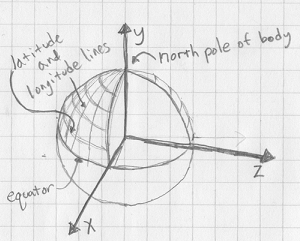
\includegraphics{KSP_body_coords.png}
\end{figure}

The Y axis of \textbf{KSP} is the only consistent thing. Imagine a ray starting in the center of the SOI body and pointing upward out through the north pole. That is the direction of the Y axis. (If you move to the SOI of a body with an inclined spin, presumably it will also change the angle of the Y axis to point in the new direction of the body's spin axis).

The X and Z axes of the coordinate grid are then consequently aligned with the equator plane of the SOI body, 90 degrees to each other. \textbf{KSP} uses a left-handed coordinate system, so the Z axis will always be rotated 90 degrees to the east of the X axis.
\begin{figure}[htbp]
\centering

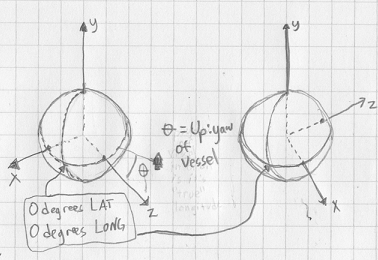
\includegraphics{KSP_body_latlong.png}
\end{figure}

However, the X and Z axes are hard to predict where they'll exactly be. They keep moving depending on where you are, to the point where it's impossible to get a fix on just which direction they'll point.


\subsection{Origin Position}
\label{math/ref_frame:origin-position}
The origin position of the \((x,y,z)\) coordinate grid in \textbf{KSP} is also a bit messy. It's usually \emph{near} but not exactly \emph{on} the current ship. \textbf{kOS} performs some conversions for you to make this a bit simpler and keep everything consistent.

Regardless of where the origin of the underlying \textbf{KSP} system is, in \textbf{kOS}, whenever a POSITION is reported, it will always be reported in a frame of reference where the origin is located at the {\hyperref[general/cpu_vessel:cpu-vessel]{\emph{\DUspan{}{CPU Vessel}}}}.

However, for the sake of VELOCITY, the origin point of all vectors is usually not SHIP, but rather it's the SOI body's center. This is because if the origin point was the SHIP, then the ship's velocity would always be zero in that frame of reference, and that would not be useful.

The makers of \textbf{kOS} are aware that this is not technically a proper frame of reference, because the origin point varies depending on if you're getting POSITION or getting VELOCITY. Fixing it at this point would break a lot of existing scripts, however.

So the rule of thumb is:
\begin{itemize}
\item {} 
For POSITION returned by \textbf{KSP}, the SHIP-RAW reference frame is used: centered on SHIP, with raw axes rotation.

\item {} 
For VELOCITY returned by \textbf{KSP}, the SOI-RAW reference frame is used: centered on SOI Body, with raw axes rotation.

\end{itemize}


\subsection{Converting}
\label{math/ref_frame:converting}
Converting between SHIP-RAW and SOI-RAW reference frames is a simple matter of adding or subtracting the SHIP:BODY:POSITION vector from the coordinate, to move the origin point. This is because both are using the same axes rotation.
\begin{itemize}
\item {} 
Any SHIP-RAW vector Minus SHIP:BODY:POSITION Gives the vector in SOI-RAW coordinates.

\item {} 
Any SOI-RAW vector Plus SHIP:BODY:POSITION Gives the vector in SHIP-RAW coordinates.

\end{itemize}


\chapter{Command Reference}
\label{commands:commands}\label{commands::doc}\label{commands:command-reference}

\section{Flight Control}
\label{commands/flight:flight-control}\label{commands/flight:flight}\label{commands/flight::doc}

\subsection{Cooked Control}
\label{commands/flight/cooked:cooked}\label{commands/flight/cooked::doc}\label{commands/flight/cooked:cooked-control}
In this style of controlling the craft, you do not steer the craft directly, but instead select a goal direction and let kOS pick the way to steer toward that goal. This method of controlling the craft consists primarily of the following two commands:
\phantomsection\label{commands/flight/cooked:lock-throttle}

\begin{fulllineitems}
\pysigline{\bfcode{LOCK~THROTTLE~TO~value.}}
This sets the main throttle of the ship to \emph{value}. Where \emph{value} is a floating point number between 0.0 and 1.0. A value of 0.0 means the throttle is idle, and a value of 1.0 means the throttle is at maximum. A value of 0.5 means the throttle is at the halfway point, and so on.

\end{fulllineitems}

\phantomsection\label{commands/flight/cooked:lock-steering}

\begin{fulllineitems}
\pysigline{\bfcode{LOCK~STEERING~TO~value.}}
This sets the direction \textbf{kOS} should point the ship where \emph{value} is a {\hyperref[math/vector:structure:VECTOR]{\emph{\code{Vector}}}} or a {\hyperref[math/direction:direction]{\emph{\DUspan{}{Direction}}}} created from a {\hyperref[math/direction:rotation]{\emph{\DUspan{}{Rotation}}}} or {\hyperref[math/direction:heading]{\emph{\DUspan{}{Heading}}}}:
\begin{quote}

{\hyperref[math/direction:rotation]{\emph{\DUspan{}{Rotation}}}}
\begin{quote}

A Rotation expressed as \code{R(pitch,yaw,roll)}. Note that pitch, yaw and roll are not based on the horizon, but based on an internal coordinate system used by \textbf{KSP} that is hard to use. Thankfully, you can force the rotation into a sensible frame of reference by adding a rotation to a known direction first.

To select a direction that is 20 degrees off from straight up:

\begin{Verbatim}[commandchars=\\\{\}]
\PYG{n}{LOCK} \PYG{n}{STEERING} \PYG{n}{TO} \PYG{n}{Up} \PYG{o}{+} \PYG{n}{R}\PYG{p}{(}\PYG{l+m+mi}{20}\PYG{p}{,}\PYG{l+m+mi}{0}\PYG{p}{,}\PYG{l+m+mi}{0}\PYG{p}{)}\PYG{p}{.}
\end{Verbatim}

To select a direction that is due east, aimed at the horizon:

\begin{Verbatim}[commandchars=\\\{\}]
\PYG{n}{LOCK} \PYG{n}{STEERING} \PYG{n}{TO} \PYG{n}{North} \PYG{o}{+} \PYG{n}{R}\PYG{p}{(}\PYG{l+m+mi}{0}\PYG{p}{,}\PYG{l+m+mi}{90}\PYG{p}{,}\PYG{l+m+mi}{0}\PYG{p}{)}\PYG{p}{.}
\end{Verbatim}

\code{UP} and \code{NORTH} are the only two predefined rotations.
\end{quote}

{\hyperref[math/direction:heading]{\emph{\DUspan{}{Heading}}}}
\begin{quote}

A heading expressed as \code{HEADING(compass, pitch)}. This will aim 30 degrees above the horizon, due south:

\begin{Verbatim}[commandchars=\\\{\}]
\PYG{n}{LOCK} \PYG{n}{STEERING} \PYG{n}{TO} \PYG{n}{HEADING}\PYG{p}{(}\PYG{l+m+mi}{180}\PYG{p}{,} \PYG{l+m+mi}{30}\PYG{p}{)}\PYG{p}{.}
\end{Verbatim}
\end{quote}

{\hyperref[math/vector:structure:VECTOR]{\emph{\code{Vector}}}}
\begin{quote}

Any vector can also be used to lock steering:

\begin{Verbatim}[commandchars=\\\{\}]
\PYG{n}{LOCK} \PYG{n}{STEERING} \PYG{n}{TO} \PYG{n}{V}\PYG{p}{(}\PYG{l+m+mi}{100}\PYG{p}{,}\PYG{l+m+mi}{50}\PYG{p}{,}\PYG{l+m+mi}{10}\PYG{p}{)}\PYG{p}{.}
\end{Verbatim}

Note that the internal coordinate system for \code{(X,Y,Z)} is quite complex to explain. To aim in the opposite of the surface velocity direction:

\begin{Verbatim}[commandchars=\\\{\}]
\PYG{n}{LOCK} \PYG{n}{STEERING} \PYG{n}{TO} \PYG{p}{(}\PYG{o}{\PYGZhy{}}\PYG{l+m+mi}{1}\PYG{p}{)} \PYG{o}{*} \PYG{n+nl}{SHIP}\PYG{p}{:}\PYG{n+nl}{VELOCITY}\PYG{p}{:}\PYG{n}{SURFACE}\PYG{p}{.}
\end{Verbatim}

The following aims at a vector which is the cross product of velocity and direction down to the SOI planet - in other words, it aims at the ``normal'' direction to the orbit:

\begin{Verbatim}[commandchars=\\\{\}]
\PYG{n}{LOCK} \PYG{n}{STEERING} \PYG{n}{TO} \PYG{n}{VCRS}\PYG{p}{(}\PYG{n+nl}{SHIP}\PYG{p}{:}\PYG{n+nl}{VELOCITY}\PYG{p}{:}\PYG{n}{ORBIT}\PYG{p}{,} \PYG{n+nl}{BODY}\PYG{p}{:}\PYG{n}{POSITION}\PYG{p}{)}\PYG{p}{.}
\end{Verbatim}
\end{quote}
\end{quote}

\end{fulllineitems}


Like all \code{LOCK} expressions, the steering and throttle continually update on their own when using this style of control. If you lock your steering to velocity, then as your velocity changes, your steering will change to match it. Unlike with other \code{LOCK} expressions, the steering and throttle are special in that the lock expression gets executed automatically all the time in the background, while other \code{LOCK} expressions only get executed when you try to read the value of the variable. The reason is that the \textbf{kOS} computer is constantly querying the lock expression multiple times per second as it adjusts the steering and throttle in the background.


\subsubsection{Unlocking controls}
\label{commands/flight/cooked:unlocking-controls}
If you \code{LOCK} the \code{THROTTLE} or \code{STEERING}, be aware that this prevents the user from manually controlling them. Until they unlock, the manual controls are prevented from working. You can free up the controls by issuing these two commands:

\begin{Verbatim}[commandchars=\\\{\}]
\PYG{n}{UNLOCK} \PYG{n}{STEERING}\PYG{p}{.}
\PYG{n}{UNLOCK} \PYG{n}{THROTTLE}\PYG{p}{.}
\end{Verbatim}

When the program ends, these automatically unlock as well, which means that to control a craft you must make sure the program doesn't end. The moment it ends it lets go of the controls.


\subsubsection{Advantages/Disadvantages}
\label{commands/flight/cooked:advantages-disadvantages}
The advantge of ``Cooked'' control is that it is simpler to write scripts for, but the disadvantage is that you have no control over the details of the motion. You can't dictate how fast or slow the craft rotates, or which axis it tries to rotate around first, and if your craft is wobbly, you can't dampen the wobbliness.


\subsection{Raw Control}
\label{commands/flight/raw:raw}\label{commands/flight/raw::doc}\label{commands/flight/raw:raw-control}
If you wish to have your kOS script manipulate a vessel's flight controls directly in a raw way, rather than relying on kOS to handle the flying for you, then this is the type of structure you will need to use to do it. This is offered as an alternative to using the combination of \code{LOCK STEERING} and \code{LOCK THROTTLE} commands. To obtain the CONTROL variable for a vessel, use its :CONTROL suffix:

\begin{Verbatim}[commandchars=\\\{\}]
\PYG{n}{SET} \PYG{n}{controlStick} \PYG{n}{to} \PYG{n+nl}{SHIP}\PYG{p}{:}\PYG{n}{CONTROL}\PYG{p}{.}
\PYG{n}{SET} \PYG{n+nl}{controlStick}\PYG{p}{:}\PYG{n}{PITCH} \PYG{n}{to} \PYG{l+m+mf}{0.2}\PYG{p}{.}
\end{Verbatim}

Unlike with so-called ``Cooked'' steering, ``raw'' steering uses the \code{SET} command, not the \code{LOCK} command. Using \code{LOCK} with these controls won't work. When controlling the ship in a raw way, you must decide how to move the controls in detail. Here is another example:

\begin{Verbatim}[commandchars=\\\{\}]
\PYG{n}{SET} \PYG{n+nl}{SHIP}\PYG{p}{:}\PYG{n+nl}{CONTROL}\PYG{p}{:}\PYG{n}{YAW} \PYG{n}{to} \PYG{l+m+mf}{0.2}\PYG{p}{.}
\end{Verbatim}

This will start pushing the ship to rotate a bit faster to the right, like pushing the \code{D} key gently. All the following values are set between \(-1\) and \(+1\). Zero means the control is neutral. You can set to values smaller in magnitude than \(-1\) and \(+1\) for gentler control:

\begin{Verbatim}[commandchars=\\\{\}]
\PYG{n}{print} \PYG{l+s}{\PYGZdq{}}\PYG{l+s}{Gently pushing forward for 3 seconds.}\PYG{l+s}{\PYGZdq{}}\PYG{p}{.}
\PYG{n}{SET} \PYG{n+nl}{SHIP}\PYG{p}{:}\PYG{n+nl}{CONTROL}\PYG{p}{:}\PYG{n}{FORE} \PYG{n}{TO} \PYG{l+m+mf}{0.2}\PYG{p}{.}
\PYG{n}{SET} \PYG{n}{now} \PYG{n}{to} \PYG{n+nl}{time}\PYG{p}{:}\PYG{n}{seconds}\PYG{p}{.}
\PYG{n}{WAIT} \PYG{n}{until} \PYG{n+nl}{time}\PYG{p}{:}\PYG{n}{seconds} \PYG{o}{\PYGZgt{}} \PYG{n}{now} \PYG{o}{+} \PYG{l+m+mf}{3.}
\PYG{n}{SET} \PYG{n+nl}{SHIP}\PYG{p}{:}\PYG{n+nl}{CONTROL}\PYG{p}{:}\PYG{n}{FORE} \PYG{n}{to} \PYG{l+m+mf}{0.0}\PYG{p}{.}

\PYG{n}{print} \PYG{l+s}{\PYGZdq{}}\PYG{l+s}{Gently Pushing leftward for 3 seconds.}\PYG{l+s}{\PYGZdq{}}\PYG{p}{.}
\PYG{n}{SET} \PYG{n+nl}{SHIP}\PYG{p}{:}\PYG{n+nl}{CONTROL}\PYG{p}{:}\PYG{n}{STARBOARD} \PYG{n}{TO} \PYG{o}{\PYGZhy{}}\PYG{l+m+mf}{0.2}\PYG{p}{.}
\PYG{n}{SET} \PYG{n}{now} \PYG{n}{to} \PYG{n+nl}{time}\PYG{p}{:}\PYG{n}{seconds}\PYG{p}{.}
\PYG{n}{WAIT} \PYG{n}{until} \PYG{n+nl}{time}\PYG{p}{:}\PYG{n}{seconds} \PYG{o}{\PYGZgt{}} \PYG{n}{now} \PYG{o}{+} \PYG{l+m+mf}{3.}
\PYG{n}{SET} \PYG{n+nl}{SHIP}\PYG{p}{:}\PYG{n+nl}{CONTROL}\PYG{p}{:}\PYG{n}{STARBOARD} \PYG{n}{to} \PYG{l+m+mf}{0.0}\PYG{p}{.}

\PYG{n}{print} \PYG{l+s}{\PYGZdq{}}\PYG{l+s}{Starting an upward rotation.}\PYG{l+s}{\PYGZdq{}}\PYG{p}{.}
\PYG{n}{SET} \PYG{n+nl}{SHIP}\PYG{p}{:}\PYG{n+nl}{CONTROL}\PYG{p}{:}\PYG{n}{PITCH} \PYG{n}{TO} \PYG{l+m+mf}{0.2}\PYG{p}{.}
\PYG{n}{SET} \PYG{n}{now} \PYG{n}{to} \PYG{n+nl}{time}\PYG{p}{:}\PYG{n}{seconds}\PYG{p}{.}
\PYG{n}{WAIT} \PYG{n}{until} \PYG{n+nl}{time}\PYG{p}{:}\PYG{n}{seconds} \PYG{o}{\PYGZgt{}} \PYG{n}{now} \PYG{o}{+} \PYG{l+m+mf}{0.5}\PYG{p}{.}
\PYG{n}{SET} \PYG{n+nl}{SHIP}\PYG{p}{:}\PYG{n+nl}{CONTROL}\PYG{p}{:}\PYG{n}{PITCH} \PYG{n}{to} \PYG{l+m+mf}{0.0}\PYG{p}{.}

\PYG{n}{print} \PYG{l+s}{\PYGZdq{}}\PYG{l+s}{Giving control back to the player now.}\PYG{l+s}{\PYGZdq{}}\PYG{p}{.}
\PYG{n}{SET} \PYG{n+nl}{SHIP}\PYG{p}{:}\PYG{n+nl}{CONTROL}\PYG{p}{:}\PYG{n}{NEUTRALIZE} \PYG{n}{to} \PYG{n}{True}\PYG{p}{.}
\end{Verbatim}

One can use {\hyperref[commands/flight/raw:ship-control-rotation]{\emph{\DUspan{}{SHIP:CONTROL:ROTATION}}}} and {\hyperref[commands/flight/raw:ship-control-translation]{\emph{\DUspan{}{SHIP:CONTROL:TRANSLATION}}}} to see the ship's current situation.


\subsubsection{Raw Flight Controls Reference}
\label{commands/flight/raw:raw-flight-controls-reference}
These ``Raw'' controls allow you the direct control of flight parameters while the current program is running.

\begin{notice}{note}{Note:}
The \code{MAINTHROTTLE} requires active engines and, of course, sufficient and appropriate fuel. The rotational controls \code{YAW}, \code{PITCH} and \code{ROW} require active reaction wheels with sufficient energy or \emph{RCS} to be ON with properly placed thrusters and appropriate fuel. The translational controls \code{FORE}, \code{STARBOARD} and \code{TOP} require \emph{RCS} to be ON with properly placed thrusters and appropriate fuel.
\end{notice}

\begin{tabulary}{\linewidth}{|L|L|L|}
\hline
\textsf{\relax 
Suffix
} & \textsf{\relax 
Type, Range
} & \textsf{\relax 
Equivalent Key
}\\
\hline
{\hyperref[commands/flight/raw:ship-control-mainthrottle]{\emph{\DUspan{}{MAINTHROTTLE}}}}
 & 
scalar {[}0,1{]}
 & 
\code{LEFT-CTRL}, \code{LEFT-SHIFT}
\\
\hline
{\hyperref[commands/flight/raw:ship-control-yaw]{\emph{\DUspan{}{YAW}}}}
 & 
scalar {[}-1,1{]}
 & 
\code{D}, \code{A}
\\
\hline
{\hyperref[commands/flight/raw:ship-control-pitch]{\emph{\DUspan{}{PITCH}}}}
 & 
scalar {[}-1,1{]}
 & 
\code{W}, \code{S}
\\
\hline
{\hyperref[commands/flight/raw:ship-control-roll]{\emph{\DUspan{}{ROLL}}}}
 & 
scalar {[}-1,1{]}
 & 
\code{Q}, \code{E}
\\
\hline
{\hyperref[commands/flight/raw:ship-control-rotation]{\emph{\DUspan{}{ROTATION}}}}
 & 
{\hyperref[math/vector:structure:VECTOR]{\emph{\code{Vector}}}}
 & 
\code{(YAW,PITCH,ROLL)}
\\
\hline
{\hyperref[commands/flight/raw:ship-control-yawtrim]{\emph{\DUspan{}{YAWTRIM}}}}
 & 
scalar {[}-1,1{]}
 & 
\code{ALT+D}, \code{ALT+A}
\\
\hline
{\hyperref[commands/flight/raw:ship-control-pitchtrim]{\emph{\DUspan{}{PITCHTRIM}}}}
 & 
scalar {[}-1,1{]}
 & 
\code{ALT+W}, \code{ALT+S}
\\
\hline
{\hyperref[commands/flight/raw:ship-control-rolltrim]{\emph{\DUspan{}{ROLLTRIM}}}}
 & 
scalar {[}-1,1{]}
 & 
\code{ALT+Q}, \code{ALT+E}
\\
\hline
{\hyperref[commands/flight/raw:ship-control-fore]{\emph{\DUspan{}{FORE}}}}
 & 
scalar {[}-1,1{]}
 & 
\code{N}, \code{H}
\\
\hline
{\hyperref[commands/flight/raw:ship-control-starboard]{\emph{\DUspan{}{STARBOARD}}}}
 & 
scalar {[}-1,1{]}
 & 
\code{L}, \code{J}
\\
\hline
{\hyperref[commands/flight/raw:ship-control-top]{\emph{\DUspan{}{TOP}}}}
 & 
scalar {[}-1,1{]}
 & 
\code{I}, \code{K}
\\
\hline
{\hyperref[commands/flight/raw:ship-control-translation]{\emph{\DUspan{}{TRANSLATION}}}}
 & 
{\hyperref[math/vector:structure:VECTOR]{\emph{\code{Vector}}}}
 & 
\code{(STARBOARD,TOP,FORE)}
\\
\hline
{\hyperref[commands/flight/raw:ship-control-wheelsteer]{\emph{\DUspan{}{WHEELSTEER}}}}
 & 
scalar {[}-1,1{]}
 & 
\code{A}, \code{D}
\\
\hline
{\hyperref[commands/flight/raw:ship-control-wheelthrottle]{\emph{\DUspan{}{WHEELTHROTTLE}}}}
 & 
scalar {[}-1,1{]}
 & 
\code{W}, \code{S}
\\
\hline
{\hyperref[commands/flight/raw:ship-control-wheelsteertrim]{\emph{\DUspan{}{WHEELSTEERTRIM}}}}
 & 
scalar {[}-1,1{]}
 & 
\code{ALT+A}, \code{ALT+D}
\\
\hline
{\hyperref[commands/flight/raw:ship-control-wheelthrottletrim]{\emph{\DUspan{}{WHEELTHROTTLETRIM}}}}
 & 
scalar {[}-1,1{]}
 & 
\code{ALT+W}, \code{ALT+S}
\\
\hline
{\hyperref[commands/flight/raw:ship-control-neutral]{\emph{\DUspan{}{NEUTRAL}}}}
 & 
boolean
 & 
Is \textbf{kOS} Controlling?
\\
\hline
{\hyperref[commands/flight/raw:ship-control-neutralize]{\emph{\DUspan{}{NEUTRALIZE}}}}
 & 
boolean
 & 
Releases Control
\\
\hline\end{tabulary}

\phantomsection\label{commands/flight/raw:ship-control-mainthrottle}

\begin{fulllineitems}
\pysigline{\bfcode{SHIP:CONTROL:MAINTHROTTLE}}
Set between 0 and 1 much like the cooked flying \code{LOCK THROTTLE} command.

\end{fulllineitems}

\phantomsection\label{commands/flight/raw:ship-control-yaw}

\begin{fulllineitems}
\pysigline{\bfcode{SHIP:CONTROL:YAW}}
This is the rotation about the ``up'' vector as the pilot faces forward. Essentially left \((-1)\) or right \((+1)\).

\end{fulllineitems}

\phantomsection\label{commands/flight/raw:ship-control-pitch}

\begin{fulllineitems}
\pysigline{\bfcode{SHIP:CONTROL:PITCH}}
Rotation about the starboard vector up \((+1)\) or down \((-1)\).

\end{fulllineitems}

\phantomsection\label{commands/flight/raw:ship-control-roll}

\begin{fulllineitems}
\pysigline{\bfcode{SHIP:CONTROL:ROLL}}
Rotation about the logintudinal axis of the ship left-wing-down \((-1)\) or left-wing-up \((+1)\).

\end{fulllineitems}

\phantomsection\label{commands/flight/raw:ship-control-rotation}

\begin{fulllineitems}
\pysigline{\bfcode{SHIP:CONTROL:ROTATION}}
This is a {\hyperref[math/vector:structure:VECTOR]{\emph{\code{Vector}}}} object containing \code{(YAW, PITCH, ROLL)} in that order.

\end{fulllineitems}

\phantomsection\label{commands/flight/raw:ship-control-yawtrim}

\begin{fulllineitems}
\pysigline{\bfcode{SHIP:CONTROL:YAWTRIM}}
Controls the \code{YAW} of the rotational trim.

\end{fulllineitems}

\phantomsection\label{commands/flight/raw:ship-control-pitchtrim}

\begin{fulllineitems}
\pysigline{\bfcode{SHIP:CONTROL:PITCHTRIM}}
Controls the \code{PITCH} of the rotational trim.

\end{fulllineitems}

\phantomsection\label{commands/flight/raw:ship-control-rolltrim}

\begin{fulllineitems}
\pysigline{\bfcode{SHIP:CONTROL:ROLLTRIM}}
Controls the \code{ROLL} of the rotational trim.

\end{fulllineitems}

\phantomsection\label{commands/flight/raw:ship-control-fore}

\begin{fulllineitems}
\pysigline{\bfcode{SHIP:CONTROL:FORE}}
Controls the translation of the ship forward \((+1)\) or backward \((-1)\).

\end{fulllineitems}

\phantomsection\label{commands/flight/raw:ship-control-starboard}

\begin{fulllineitems}
\pysigline{\bfcode{SHIP:CONTROL:STARBOARD}}
Controls the translation of the ship to the right \((+1)\) or left \((-1)\) from the pilot's perspective.

\end{fulllineitems}

\phantomsection\label{commands/flight/raw:ship-control-top}

\begin{fulllineitems}
\pysigline{\bfcode{SHIP:CONTROL:TOP}}
Controls the translation of the ship up \((+1)\) or down \((-1)\) from the pilot's perspective.

\end{fulllineitems}

\phantomsection\label{commands/flight/raw:ship-control-translation}

\begin{fulllineitems}
\pysigline{\bfcode{SHIP:CONTROL:TRANSLATION}}
Controls the translation as a {\hyperref[math/vector:structure:VECTOR]{\emph{\code{Vector}}}} \code{(STARBOARD, TOP, FORE)}.

\end{fulllineitems}

\phantomsection\label{commands/flight/raw:ship-control-wheelsteer}

\begin{fulllineitems}
\pysigline{\bfcode{SHIP:CONTROL:WHEELSTEER}}
Turns the wheels left \((-1)\) or right \((+1)\).

\end{fulllineitems}

\phantomsection\label{commands/flight/raw:ship-control-wheelthrottle}

\begin{fulllineitems}
\pysigline{\bfcode{SHIP:CONTROL:WHEELTHROTTLE}}
Controls the wheels to move the ship forward \((+1)\) or backward \((-1)\) while on the ground.

\end{fulllineitems}

\phantomsection\label{commands/flight/raw:ship-control-wheelsteertrim}

\begin{fulllineitems}
\pysigline{\bfcode{SHIP:CONTROL:WHEELSTEERTRIM}}
Controls the trim of the wheel steering.

\end{fulllineitems}

\phantomsection\label{commands/flight/raw:ship-control-wheelthrottletrim}

\begin{fulllineitems}
\pysigline{\bfcode{SHIP:CONTROL:WHEELTHROTTLETRIM}}
Controls the trim of the wheel throttle.

\end{fulllineitems}

\phantomsection\label{commands/flight/raw:ship-control-neutral}

\begin{fulllineitems}
\pysigline{\bfcode{SHIP:CONTROL:NEUTRAL}}
Returns true or false depending if \textbf{kOS} has any set controls. \emph{This is not settable.}

\end{fulllineitems}

\phantomsection\label{commands/flight/raw:ship-control-neutralize}

\begin{fulllineitems}
\pysigline{\bfcode{SHIP:CONTROL:NEUTRALIZE}}
This causes manual control to let go. When set to true, \textbf{kOS} lets go of the controls and allows the player to manually control them again. \emph{This is not gettable.}

\end{fulllineitems}



\subsubsection{Unlocking controls}
\label{commands/flight/raw:unlocking-controls}
Setting any one of \code{SHIP:CONTROL} values will prevent player from manipulating that specific control manually. Other controls will not be locked.
To free any single control, set it back to zero. To give all controls back to the player you must execute:

\begin{Verbatim}[commandchars=\\\{\}]
\PYG{n}{SET} \PYG{n+nl}{SHIP}\PYG{p}{:}\PYG{n+nl}{CONTROL}\PYG{p}{:}\PYG{n}{NEUTRALIZE} \PYG{n}{to} \PYG{n}{TRUE}\PYG{p}{.}
\end{Verbatim}


\subsubsection{Advantages/Disadvantages}
\label{commands/flight/raw:advantages-disadvantages}
The control over \emph{RCS} translation requires the use of Raw control. Also, with raw control you can choose how gentle to be with the controls and it can be possible to control wobbly craft better with raw control than with cooked control.


\subsection{Pilot Input}
\label{commands/flight/pilot::doc}\label{commands/flight/pilot:pilot-input}\label{commands/flight/pilot:pilot}
This is not, strictly speaking, a method of controlling the craft. ``Pilot'' controls are a way to read the input from the pilot. Most of these controls share the same name as their flight control, prefixed with \code{PILOT} (eg \code{YAW} and \code{PILOTYAW})  the one exception to this is the \code{PILOTMAINTHROTTLE}. This suffix has a setter and allows you to change the behavior of the throttle that persists even after the current program ends:

\begin{Verbatim}[commandchars=\\\{\}]
\PYG{n}{SET} \PYG{n+nl}{SHIP}\PYG{p}{:}\PYG{n+nl}{CONTROL}\PYG{p}{:}\PYG{n}{PILOTMAINTHROTTLE} \PYG{n}{TO} \PYG{l+m+mf}{0.}
\end{Verbatim}

Will ensure that the throttle will be 0 when execution stops. These suffixes allow you to read the input given to the system by the user.
\index{Control {[}struct{]}}

\begin{fulllineitems}
\phantomsection\label{commands/flight/pilot:structure:CONTROL}\pysigline{\strong{structure }\bfcode{Control}}
\end{fulllineitems}


\begin{tabulary}{\linewidth}{|L|L|L|}
\hline
\textsf{\relax 
Suffix
} & \textsf{\relax 
Type, Range
} & \textsf{\relax 
Equivalent Key
}\\
\hline
{\hyperref[commands/flight/pilot:ship-control-pilotmainthrottle]{\emph{\DUspan{}{PILOTMAINTHROTTLE}}}}
 & 
scalar {[}0,1{]}
 & 
\code{LEFT-CTRL}, \code{LEFT-SHIFT}
\\
\hline
{\hyperref[commands/flight/pilot:ship-control-pilotyaw]{\emph{\DUspan{}{PILOTYAW}}}}
 & 
scalar {[}-1,1{]}
 & 
\code{D}, \code{A}
\\
\hline
{\hyperref[commands/flight/pilot:ship-control-pilotpitch]{\emph{\DUspan{}{PILOTPITCH}}}}
 & 
scalar {[}-1,1{]}
 & 
\code{W}, \code{S}
\\
\hline
{\hyperref[commands/flight/pilot:ship-control-pilotroll]{\emph{\DUspan{}{PILOTROLL}}}}
 & 
scalar {[}-1,1{]}
 & 
\code{Q}, \code{E}
\\
\hline
{\hyperref[commands/flight/pilot:ship-control-pilotrotation]{\emph{\DUspan{}{PILOTROTATION}}}}
 & 
{\hyperref[math/vector:structure:VECTOR]{\emph{\code{Vector}}}}
 & 
\code{(YAW,PITCH,ROLL)}
\\
\hline
{\hyperref[commands/flight/pilot:ship-control-pilotyawtrim]{\emph{\DUspan{}{PILOTYAWTRIM}}}}
 & 
scalar {[}-1,1{]}
 & 
\code{ALT+D}, \code{ALT+A}
\\
\hline
{\hyperref[commands/flight/pilot:ship-control-pilotpitchtrim]{\emph{\DUspan{}{PILOTPITCHTRIM}}}}
 & 
scalar {[}-1,1{]}
 & 
\code{ALT+W}, \code{ALT+S}
\\
\hline
{\hyperref[commands/flight/pilot:ship-control-pilotrolltrim]{\emph{\DUspan{}{PILOTROLLTRIM}}}}
 & 
scalar {[}-1,1{]}
 & 
\code{ALT+Q}, \code{ALT+E}
\\
\hline
{\hyperref[commands/flight/pilot:ship-control-pilotfore]{\emph{\DUspan{}{PILOTFORE}}}}
 & 
scalar {[}-1,1{]}
 & 
\code{N}, \code{H}
\\
\hline
{\hyperref[commands/flight/pilot:ship-control-pilotstarboard]{\emph{\DUspan{}{PILOTSTARBOARD}}}}
 & 
scalar {[}-1,1{]}
 & 
\code{L}, \code{J}
\\
\hline
{\hyperref[commands/flight/pilot:ship-control-pilottop]{\emph{\DUspan{}{PILOTTOP}}}}
 & 
scalar {[}-1,1{]}
 & 
\code{I}, \code{K}
\\
\hline
{\hyperref[commands/flight/pilot:ship-control-pilottranslation]{\emph{\DUspan{}{PILOTTRANSLATION}}}}
 & 
{\hyperref[math/vector:structure:VECTOR]{\emph{\code{Vector}}}}
 & 
\code{(STARBOARD,TOP,FORE)}
\\
\hline
{\hyperref[commands/flight/pilot:ship-control-pilotwheelsteer]{\emph{\DUspan{}{PILOTWHEELSTEER}}}}
 & 
scalar {[}-1,1{]}
 & 
\code{A}, \code{D}
\\
\hline
{\hyperref[commands/flight/pilot:ship-control-pilotwheelthrottle]{\emph{\DUspan{}{PILOTWHEELTHROTTLE}}}}
 & 
scalar {[}-1,1{]}
 & 
\code{W}, \code{S}
\\
\hline
{\hyperref[commands/flight/pilot:ship-control-pilotwheelsteertrim]{\emph{\DUspan{}{PILOTWHEELSTEERTRIM}}}}
 & 
scalar {[}-1,1{]}
 & 
\code{ALT+A}, \code{ALT+D}
\\
\hline
{\hyperref[commands/flight/pilot:ship-control-pilotwheelthrottletrim]{\emph{\DUspan{}{PILOTWHEELTHROTTLETRIM}}}}
 & 
scalar {[}-1,1{]}
 & 
\code{ALT+W}, \code{ALT+S}
\\
\hline
{\hyperref[commands/flight/pilot:ship-control-pilotneutral]{\emph{\DUspan{}{PILOTNEUTRAL}}}}
 & 
boolean
 & 
Is \textbf{kOS} Controlling?
\\
\hline\end{tabulary}

\phantomsection\label{commands/flight/pilot:ship-control-pilotmainthrottle}

\begin{fulllineitems}
\pysigline{\bfcode{SHIP:CONTROL:PILOTMAINTHROTTLE}}
Returns the pilot's input for the throttle. This is the only \code{PILOT} variable that is settable and is used to set the throttle upon termination of the current \textbf{kOS} program.

\end{fulllineitems}

\phantomsection\label{commands/flight/pilot:ship-control-pilotyaw}

\begin{fulllineitems}
\pysigline{\bfcode{SHIP:CONTROL:PILOTYAW}}
Returns the pilot's rotation input about the ``up'' vector as the pilot faces forward. Essentially left \((-1)\) or right \((+1)\).

\end{fulllineitems}

\phantomsection\label{commands/flight/pilot:ship-control-pilotpitch}

\begin{fulllineitems}
\pysigline{\bfcode{SHIP:CONTROL:PILOTPITCH}}
Returns the pilot's rotation input  about the starboard vector up \((+1)\) or down \((-1)\).

\end{fulllineitems}

\phantomsection\label{commands/flight/pilot:ship-control-pilotroll}

\begin{fulllineitems}
\pysigline{\bfcode{SHIP:CONTROL:PILOTROLL}}
Returns the pilot's rotation input  about the logintudinal axis of the ship left-wing-down \((-1)\) or left-wing-up \((+1)\).

\end{fulllineitems}

\phantomsection\label{commands/flight/pilot:ship-control-pilotrotation}

\begin{fulllineitems}
\pysigline{\bfcode{SHIP:CONTROL:PILOTROTATION}}
Returns the pilot's rotation input as a {\hyperref[math/vector:structure:VECTOR]{\emph{\code{Vector}}}} object containing \code{(YAW, PITCH, ROLL)} in that order.

\end{fulllineitems}

\phantomsection\label{commands/flight/pilot:ship-control-pilotyawtrim}

\begin{fulllineitems}
\pysigline{\bfcode{SHIP:CONTROL:PILOTYAWTRIM}}
Returns the pilot's input for the \code{YAW} of the rotational trim.

\end{fulllineitems}

\phantomsection\label{commands/flight/pilot:ship-control-pilotpitchtrim}

\begin{fulllineitems}
\pysigline{\bfcode{SHIP:CONTROL:PILOTPITCHTRIM}}
Returns the pilot's input for the \code{PITCH} of the rotational trim.

\end{fulllineitems}

\phantomsection\label{commands/flight/pilot:ship-control-pilotrolltrim}

\begin{fulllineitems}
\pysigline{\bfcode{SHIP:CONTROL:PILOTROLLTRIM}}
Returns the pilot's input for the \code{ROLL} of the rotational trim.

\end{fulllineitems}

\phantomsection\label{commands/flight/pilot:ship-control-pilotfore}

\begin{fulllineitems}
\pysigline{\bfcode{SHIP:CONTROL:PILOTFORE}}
Returns the the pilot's input for the translation of the ship forward \((+1)\) or backward \((-1)\).

\end{fulllineitems}

\phantomsection\label{commands/flight/pilot:ship-control-pilotstarboard}

\begin{fulllineitems}
\pysigline{\bfcode{SHIP:CONTROL:PILOTSTARBOARD}}
Returns the the pilot's input for the translation of the ship to the right \((+1)\) or left \((-1)\) from the pilot's perspective.

\end{fulllineitems}

\phantomsection\label{commands/flight/pilot:ship-control-pilottop}

\begin{fulllineitems}
\pysigline{\bfcode{SHIP:CONTROL:PILOTTOP}}
Returns the the pilot's input for the translation of the ship up \((+1)\) or down \((-1)\) from the pilot's perspective.

\end{fulllineitems}

\phantomsection\label{commands/flight/pilot:ship-control-pilottranslation}

\begin{fulllineitems}
\pysigline{\bfcode{SHIP:CONTROL:PILOTTRANSLATION}}
Returns the the pilot's input for translation as a {\hyperref[math/vector:structure:VECTOR]{\emph{\code{Vector}}}} \code{(STARBOARD, TOP, FORE)}.

\end{fulllineitems}

\phantomsection\label{commands/flight/pilot:ship-control-pilotwheelsteer}

\begin{fulllineitems}
\pysigline{\bfcode{SHIP:CONTROL:PILOTWHEELSTEER}}
Returns the the pilot's input for wheel steering left \((-1)\) or right \((+1)\).

\end{fulllineitems}

\phantomsection\label{commands/flight/pilot:ship-control-pilotwheelthrottle}

\begin{fulllineitems}
\pysigline{\bfcode{SHIP:CONTROL:PILOTWHEELTHROTTLE}}
Returns the the pilot's input for the wheels to move the ship forward \((+1)\) or backward \((-1)\) while on the ground.

\end{fulllineitems}

\phantomsection\label{commands/flight/pilot:ship-control-pilotwheelsteertrim}

\begin{fulllineitems}
\pysigline{\bfcode{SHIP:CONTROL:PILOTWHEELSTEERTRIM}}
Returns the the pilot's input for the trim of the wheel steering.

\end{fulllineitems}

\phantomsection\label{commands/flight/pilot:ship-control-pilotwheelthrottletrim}

\begin{fulllineitems}
\pysigline{\bfcode{SHIP:CONTROL:PILOTWHEELTHROTTLETRIM}}
Returns the the pilot's input for the trim of the wheel throttle.

\end{fulllineitems}

\phantomsection\label{commands/flight/pilot:ship-control-pilotneutral}

\begin{fulllineitems}
\pysigline{\bfcode{SHIP:CONTROL:PILOTNEUTRAL}}
Returns true or false if the pilot is active or not.

\end{fulllineitems}


Be aware that \textbf{kOS} can't control a control at the same time that a player controls it. If \textbf{kOS} is taking control of the yoke, then the player can't manually control it. Remember to run:

\begin{Verbatim}[commandchars=\\\{\}]
\PYG{n}{SET} \PYG{n+nl}{SHIP}\PYG{p}{:}\PYG{n+nl}{CONTROL}\PYG{p}{:}\PYG{n}{NEUTRALIZE} \PYG{n}{TO} \PYG{n}{TRUE}\PYG{p}{.}
\end{Verbatim}

after the script is done using the controls, or the player will be locked out of control.


\subsection{Ship Systems}
\label{commands/flight/systems:ship-systems}\label{commands/flight/systems::doc}\label{commands/flight/systems:systems}\phantomsection\label{commands/flight/systems:controlfrom}\begin{quote}

e.g.:

\begin{Verbatim}[commandchars=\\\{\}]
\PYG{n}{set} \PYG{n}{somepart} \PYG{n}{to} \PYG{n+nl}{ship}\PYG{p}{:}\PYG{n}{partstagged}\PYG{p}{(}\PYG{l+s}{\PYGZdq{}}\PYG{l+s}{my favorite docking port}\PYG{l+s}{\PYGZdq{}}\PYG{p}{)}\PYG{p}{[}\PYG{l+m+mi}{0}\PYG{p}{]}\PYG{p}{.}
\PYG{n+nl}{somepart}\PYG{p}{:}\PYG{n}{CONTROLFROM}\PYG{p}{(}\PYG{p}{)}\PYG{p}{.}
\end{Verbatim}

If you have a handle on a part, from \code{LIST PARTS}, you can select that part to set the orientation of the craft, just like using the ``control from here'' in the right-click menu in the game. For more information see {\hyperref[structures/vessels/part:attribute:PART:CONTROLFROM]{\emph{\code{Part:CONTROLFROM}}}}.
All vessels must have at least one ``control from''
part on them somewhere, which is why there's no mechanism for un-setting
the ``control from'' setting other than to pick another part and set it
to that part instead.
\end{quote}
\index{RCS}

\begin{fulllineitems}
\phantomsection\label{commands/flight/systems:global:RCS}\pysigline{\bfcode{RCS}}~\begin{quote}\begin{description}
\item[{Access}] \leavevmode
Toggle ON/OFF

\end{description}\end{quote}

Turns the RCS \textbf{on} or \textbf{off}, like using \code{R} at the keyboard:

\begin{Verbatim}[commandchars=\\\{\}]
\PYG{n}{RCS} \PYG{n}{ON}\PYG{p}{.}
\end{Verbatim}

\end{fulllineitems}

\index{SAS}

\begin{fulllineitems}
\phantomsection\label{commands/flight/systems:global:SAS}\pysigline{\bfcode{SAS}}~\begin{quote}\begin{description}
\item[{Access}] \leavevmode
Toggle ON/OFF

\end{description}\end{quote}

Turns the SAS \textbf{on} or \textbf{off}, like using \code{T} at the keybaord:

\begin{Verbatim}[commandchars=\\\{\}]
\PYG{n}{SAS} \PYG{n}{ON}\PYG{p}{.}
\end{Verbatim}

\end{fulllineitems}

\phantomsection\label{commands/flight/systems:sasmode}

\begin{fulllineitems}
\pysigline{\bfcode{SET~SASMODE~TO~value.}}~\begin{quote}\begin{description}
\item[{Access}] \leavevmode
Get/Set

\item[{Type}] \leavevmode
string

\end{description}\end{quote}

Getting this variable will return the currently selected mode.  Where \code{value} is one of the valid strings listed below, this will set the stock SAS mode for the cpu vessel:

\begin{Verbatim}[commandchars=\\\{\}]
\PYG{n}{SET} \PYG{n}{SASMODE} \PYG{n}{TO} \PYG{n}{value}\PYG{p}{.}
\end{Verbatim}

It is the equivalent to clicking on the buttons next to the nav ball while manually piloting the craft, and will respect the current mode of the nav ball (orbital, surface, or target velocity).  Valid strings for \code{value} are \code{"PROGRADE"}, \code{"RETROGRADE"}, \code{"NORMAL"}, \code{"ANTINORMAL"}, \code{"RADIALOUT"}, \code{"RADIALIN"}, \code{"TARGET"}, \code{"ANTITARGET"}, \code{MANEUVER}, \code{"STABILITYASSIST"}, and \code{"STABILITY"}.  A null or empty string will default to stability assist mode, however any other invalid string will throw an exception.  This feature will respect career mode limitations, and will throw an exception if the current vessel is not able to use the mode passed to the command.  An exception is also thrown if \code{"TARGET"} or \code{"ANTITARGET"} are used, but no target is selected.

\end{fulllineitems}


\begin{notice}{warning}{Warning:}
SASMODE does not work with RemoteTech

Due to the way that RemoteTech disables flight control input, the built in SAS modes do not function properly when there is no connection to the KSC or a Command Center.  If you are writing scripts for use with RemoteTech, make sure to take this into account.
\end{notice}
\index{LIGHTS}

\begin{fulllineitems}
\phantomsection\label{commands/flight/systems:global:LIGHTS}\pysigline{\bfcode{LIGHTS}}~\begin{quote}\begin{description}
\item[{Access}] \leavevmode
Toggle ON/OFF

\end{description}\end{quote}

Turns the lights \textbf{on} or \textbf{off}, like using the \code{U} key at the keyboard:

\begin{Verbatim}[commandchars=\\\{\}]
\PYG{n}{LIGHTS} \PYG{n}{ON}\PYG{p}{.}
\end{Verbatim}

\end{fulllineitems}

\index{BRAKES}

\begin{fulllineitems}
\phantomsection\label{commands/flight/systems:global:BRAKES}\pysigline{\bfcode{BRAKES}}~\begin{quote}\begin{description}
\item[{Access}] \leavevmode
Toggle ON/OFF

\end{description}\end{quote}

Turns the brakes \textbf{on} or \textbf{off}, like clicking the brakes button, though \emph{not} like using the \code{B} key, because they stay on:

\begin{Verbatim}[commandchars=\\\{\}]
\PYG{n}{BRAKES} \PYG{n}{ON}\PYG{p}{.}
\end{Verbatim}

\end{fulllineitems}

\index{TARGET}

\begin{fulllineitems}
\phantomsection\label{commands/flight/systems:global:TARGET}\pysigline{\bfcode{TARGET}}~\begin{quote}\begin{description}
\item[{Access}] \leavevmode
Get/Set

\item[{Type}] \leavevmode
string

\end{description}\end{quote}

Where \code{name} is the name of a target vessel or planet, this will set the current target:

\begin{Verbatim}[commandchars=\\\{\}]
\PYG{n}{SET} \PYG{n}{TARGET} \PYG{n}{TO} \PYG{n}{name}\PYG{p}{.}
\end{Verbatim}

\end{fulllineitems}


Note that the above options also can refer to a different vessel besides the current ship, for example, \code{TARGET:THROTTLE} to read the target's throttle. But not all ``set'' or ``lock'' options will work with a different vessel other than the current one, because there's no authority to control a craft the current program is not attached to.


\subsection{Time Warping}
\label{commands/flight/warp::doc}\label{commands/flight/warp:time-warping}\label{commands/flight/warp:warp}\index{WARP}

\begin{fulllineitems}
\phantomsection\label{commands/flight/warp:global:WARP}\pysigline{\bfcode{WARP}}
You may use the WARPTO(time) function to automatically warp to the specified time (given in seconds game universal time).  If you need more precise control, you can use the other options below.:

\begin{Verbatim}[commandchars=\\\{\}]
\PYG{n}{WARPTO}\PYG{p}{(}\PYG{n+nl}{TIME}\PYG{p}{:}\PYG{n}{SECONDS} \PYG{o}{+} \PYG{l+m+mi}{60} \PYG{o}{*} \PYG{l+m+mi}{10}\PYG{p}{)}\PYG{p}{.} \PYG{c+c1}{// warp to a time 10 minutes in the future}
\end{Verbatim}

The {\hyperref[commands/flight/warp:global:WARP]{\emph{\code{WARP}}}} global variable can be set to change the game warp to a value between 0 and 7 (for rails warp) or 0 to 3 (for physics warp):

\begin{Verbatim}[commandchars=\\\{\}]
\PYG{n}{SET} \PYG{n}{WARP} \PYG{n}{TO} \PYG{l+m+mf}{5.} \PYG{c+c1}{// Sets warp to 1000x}
\PYG{n}{SET} \PYG{n}{WARP} \PYG{n}{TO} \PYG{l+m+mf}{0.} \PYG{c+c1}{// Sets warp to 1x (real time)}
\end{Verbatim}

You may also choose which warp mode you wish the WARP command
to invoke- physics warp (capped at 4x) or rails warp:

\begin{Verbatim}[commandchars=\\\{\}]
\PYG{n}{SET} \PYG{n}{WARPMODE} \PYG{n}{TO} \PYG{l+s}{\PYGZdq{}}\PYG{l+s}{PHYSICS}\PYG{l+s}{\PYGZdq{}}\PYG{p}{.}
\PYG{n}{SET} \PYG{n}{WARPMODE} \PYG{n}{TO} \PYG{l+s}{\PYGZdq{}}\PYG{l+s}{RAILS}\PYG{l+s}{\PYGZdq{}}\PYG{p}{.}
\end{Verbatim}

WARPMODE can be set to a string to choose the warp.  It must be
one of the two strings mentioned above.

The difference is the same as that experienced in the game between
physics warp and `rails' warp (sometimes called `time warp') although
that term is confusingly ambiguous.

\end{fulllineitems}



\begin{threeparttable}
\capstart\caption{RAILS WARP MODES}
\label{commands/flight/warp:id1}
\begin{tabulary}{\linewidth}{|L|L|}
\hline
\textsf{\relax 
MODE
} & \textsf{\relax 
MEANING
}\\
\hline
0
 & 
1x
\\
\hline
1
 & 
5x
\\
\hline
2
 & 
10x
\\
\hline
3
 & 
50x
\\
\hline
4
 & 
100x
\\
\hline
5
 & 
1000x
\\
\hline
6
 & 
10000x
\\
\hline
7
 & 
100000x
\\
\hline\end{tabulary}

\end{threeparttable}



\begin{threeparttable}
\capstart\caption{PHYSICS WARP MODES}
\label{commands/flight/warp:id2}
\begin{tabulary}{\linewidth}{|L|L|}
\hline
\textsf{\relax 
MODE
} & \textsf{\relax 
MEANING
}\\
\hline
0
 & 
1x
\\
\hline
1
 & 
2x
\\
\hline
2
 & 
3x
\\
\hline
3
 & 
4x
\\
\hline\end{tabulary}

\end{threeparttable}


Unless otherwise stated, all controls that a \textbf{kOS} CPU attempts will be done on the {\hyperref[general/cpu_vessel:cpu-vessel]{\emph{\DUspan{}{CPU Vessel}}}}. There are three styles of control:
\begin{description}
\item[{{\hyperref[commands/flight/cooked:cooked]{\emph{\DUspan{}{Cooked}}}}}] \leavevmode
Give a goal direction to seek, and let \textbf{kOS} find the way to maneuver toward it.

\item[{{\hyperref[commands/flight/raw:raw]{\emph{\DUspan{}{Raw}}}}}] \leavevmode
Control the craft just like a manual pilot would do from a keyboard or joystick.

\item[{{\hyperref[commands/flight/pilot:pilot]{\emph{\DUspan{}{Pilot}}}}}] \leavevmode
This is the stock way of controlling craft, the state of which can be read in \textbf{KerboScript}.

\end{description}

\begin{notice}{warning}{Warning:}
\textbf{SAS OVERRIDES kOS}

With the current implementation of flight control, you may now leave \code{SAS} turned on in \code{"STABILITYASSIST"} mode, and it will not override \textbf{kOS}`s attempts to steer the ship. However, it will fight and/or override \textbf{kOS}`s attempts to steer when using any other mode.  In order for \textbf{kOS} to be able to turn the ship in other modes, you need to set \code{SAS OFF} or \code{SET SASMODE TO "STABILITYASSIST"}. You should take care in your scripts to manage the use of \code{SAS} and \code{SASMODE} appropriately. It is common for people writing \textbf{kOS} scripts to explicitly start them with a use of the \code{SAS OFF} and/or \code{SET SASMODE TO "STABILITYASSIST"} commands just in case you forgot to turn it off before running the script.  You could also store the current state in a temporary variable, and re-set it at the conclusion of your script.
\end{notice}


\section{Predictions of Flight Path}
\label{commands/prediction::doc}\label{commands/prediction:predictions-of-flight-path}
\begin{notice}{note}{Note:}
\textbf{Manipulating the maneuver nodes}

To alter the maneuver nodes on a vessel's flight plan, use the ADD and REMOVE commands as described on the {\hyperref[structures/vessels/node:maneuver-node]{\emph{\DUspan{}{maneuver node manipulation page}}}}.

Using the Add and Remove commands as described on that page, you may alter the flight plan of the CPU\_vessel, however kOS does not automatically execute the nodes. You still have to write the code to decide how to successfully execute a planned maneuver node.
\end{notice}

\begin{notice}{warning}{Warning:}
Be aware that a limitation of KSP makes it so that some vessels'
manuever node systems cannot be accessed.  KSP appears to limit the
maneuver node system to only functioning on the current PLAYER
vessel, under the presumption that its the only vessel that needs
them, as ever other vessel cannot be manuevered. kOS can manuever a
vessel that is not the player vessel, but it cannot overcome this
limitation of the base game that unloads the maneuver node system
for other vessels.

Be aware that the effect this has is that when you try to predict
another vessel's position, it will sometimes give you answers that
presume that other vessel will be purely drifting, and not following
its maneuver nodes.
\end{notice}

The following prediction functions do take into account the future maneuver nodes planned, and operate under the assumption that they will be executed as planned.

These return predicted information about the future position and velocity of an object.
\index{POSITIONAT()}

\begin{fulllineitems}
\phantomsection\label{commands/prediction:function:POSITIONAT}\pysiglinewithargsret{\bfcode{POSITIONAT}}{orbitable,time}{}~\begin{quote}\begin{description}
\item[{Parameters}] \leavevmode\begin{itemize}
\item {} 
\textbf{\texttt{orbitable}} -- A {\hyperref[structures/vessels/vessel:structure:VESSEL]{\emph{\code{Vessel}}}}, {\hyperref[structures/celestial_bodies/body:structure:BODY]{\emph{\code{Body}}}} or other {\hyperref[structures/orbits/orbitable:structure:ORBITABLE]{\emph{\code{Orbitable}}}} object

\item {} 
\textbf{\texttt{time}} -- Time of prediction

\end{itemize}

\item[{Type orbitable}] \leavevmode
{\hyperref[structures/orbits/orbitable:structure:ORBITABLE]{\emph{\code{Orbitable}}}}

\item[{Type time}] \leavevmode
{\hyperref[structures/misc/time:structure:TIMESPAN]{\emph{\code{TimeSpan}}}}

\item[{Returns}] \leavevmode
A position {\hyperref[math/vector:structure:VECTOR]{\emph{\code{Vector}}}} expressed as the coordinates in the {\hyperref[math/ref_frame:ship-raw]{\emph{\DUspan{}{ship-center-raw-rotation}}}} frame

\end{description}\end{quote}

Returns a prediction of where the {\hyperref[structures/orbits/orbitable:structure:ORBITABLE]{\emph{\code{Orbitable}}}} will be at some {\hyperref[structures/misc/time:timestamp]{\emph{\DUspan{}{universal Timestamp}}}}. If the {\hyperref[structures/orbits/orbitable:structure:ORBITABLE]{\emph{\code{Orbitable}}}} is a {\hyperref[structures/vessels/vessel:structure:VESSEL]{\emph{\code{Vessel}}}}, and the {\hyperref[structures/vessels/vessel:structure:VESSEL]{\emph{\code{Vessel}}}} has planned {\hyperref[structures/vessels/node:maneuver-node]{\emph{\DUspan{}{maneuver nodes}}}}, the prediction assumes they will be executed exactly as planned.

\end{fulllineitems}

\index{VELOCITYAT()}

\begin{fulllineitems}
\phantomsection\label{commands/prediction:function:VELOCITYAT}\pysiglinewithargsret{\bfcode{VELOCITYAT}}{orbitable,time}{}~\begin{quote}\begin{description}
\item[{Parameters}] \leavevmode\begin{itemize}
\item {} 
\textbf{\texttt{orbitable}} -- A {\hyperref[structures/vessels/vessel:structure:VESSEL]{\emph{\code{Vessel}}}}, {\hyperref[structures/celestial_bodies/body:structure:BODY]{\emph{\code{Body}}}} or other {\hyperref[structures/orbits/orbitable:structure:ORBITABLE]{\emph{\code{Orbitable}}}} object

\item {} 
\textbf{\texttt{time}} -- Time of prediction

\end{itemize}

\item[{Type orbitable}] \leavevmode
{\hyperref[structures/orbits/orbitable:structure:ORBITABLE]{\emph{\code{Orbitable}}}}

\item[{Type time}] \leavevmode
{\hyperref[structures/misc/time:structure:TIMESPAN]{\emph{\code{TimeSpan}}}}

\item[{Returns}] \leavevmode
An {\hyperref[structures/orbits/orbitablevelocity:orbitablevelocity]{\emph{\DUspan{}{ObitalVelocity}}}} structure.

\end{description}\end{quote}

Returns a prediction of what the {\hyperref[structures/orbits/orbitable:orbitable]{\emph{\DUspan{}{Orbitable's}}}} velocity will be at some {\hyperref[structures/misc/time:timestamp]{\emph{\DUspan{}{universal Timestamp}}}}. If the {\hyperref[structures/orbits/orbitable:structure:ORBITABLE]{\emph{\code{Orbitable}}}} is a {\hyperref[structures/vessels/vessel:structure:VESSEL]{\emph{\code{Vessel}}}}, and the {\hyperref[structures/vessels/vessel:structure:VESSEL]{\emph{\code{Vessel}}}} has planned \code{maneuver nodes}, the prediction assumes they will be executed exactly as planned.

\end{fulllineitems}

\index{ORBITAT()}

\begin{fulllineitems}
\phantomsection\label{commands/prediction:function:ORBITAT}\pysiglinewithargsret{\bfcode{ORBITAT}}{orbitable,time}{}~\begin{quote}\begin{description}
\item[{Parameters}] \leavevmode\begin{itemize}
\item {} 
\textbf{\texttt{orbitable}} -- A {\hyperref[structures/vessels/vessel:vessel]{\emph{\DUspan{}{Vessel}}}}, {\hyperref[structures/celestial_bodies/body:structure:BODY]{\emph{\code{Body}}}} or other {\hyperref[structures/orbits/orbitable:structure:ORBITABLE]{\emph{\code{Orbitable}}}} object

\item {} 
\textbf{\texttt{time}} -- Time of prediction

\end{itemize}

\item[{Type orbitable}] \leavevmode
{\hyperref[structures/orbits/orbitable:structure:ORBITABLE]{\emph{\code{Orbitable}}}}

\item[{Type time}] \leavevmode
{\hyperref[structures/misc/time:structure:TIMESPAN]{\emph{\code{TimeSpan}}}}

\item[{Returns}] \leavevmode
An {\hyperref[structures/orbits/orbit:structure:ORBIT]{\emph{\code{Orbit}}}} structure.

\end{description}\end{quote}

Returns the {\hyperref[structures/orbits/orbit:orbit]{\emph{\DUspan{}{Orbit patch}}}} where the {\hyperref[structures/orbits/orbitable:structure:ORBITABLE]{\emph{\code{Orbitable}}}} object is predicted to be at some {\hyperref[structures/misc/time:timestamp]{\emph{\DUspan{}{universal Timestamp}}}}. If the {\hyperref[structures/orbits/orbitable:structure:ORBITABLE]{\emph{\code{Orbitable}}}} is a {\hyperref[structures/vessels/vessel:structure:VESSEL]{\emph{\code{Vessel}}}}, and the {\hyperref[structures/vessels/vessel:structure:VESSEL]{\emph{\code{Vessel}}}} has planned {\hyperref[structures/vessels/node:maneuver-node]{\emph{\DUspan{}{maneuver nodes}}}}, the prediction assumes they will be executed exactly as planned.

\end{fulllineitems}


Examples:

\begin{Verbatim}[commandchars=\\\{\}]
\PYG{c+c1}{//kOS}
\PYG{c+c1}{// test the future position and velocity prediction.}
\PYG{c+c1}{// Draws a position and velocity vector at a future predicted time.}

\PYG{n}{declare} \PYG{n}{parameter} \PYG{n}{item}\PYG{p}{.} \PYG{c+c1}{// thing to predict for, i.e. SHIP.}
\PYG{n}{declare} \PYG{n}{parameter} \PYG{n}{offset}\PYG{p}{.} \PYG{c+c1}{// how much time into the future to predict.}
\PYG{n}{declare} \PYG{n}{parameter} \PYG{n}{velScale}\PYG{p}{.} \PYG{c+c1}{// how big to draw the velocity vectors.}
              \PYG{c+c1}{// If they\PYGZsq{}re far from the camera you should draw them bigger.}


\PYG{n}{set} \PYG{n}{predictUT} \PYG{n}{to} \PYG{n}{time} \PYG{o}{+} \PYG{n}{offset}\PYG{p}{.}
\PYG{n}{set} \PYG{n}{stopProg} \PYG{n}{to} \PYG{n+nb}{false}\PYG{p}{.}

\PYG{n}{set} \PYG{n}{futurePos} \PYG{n}{to} \PYG{n}{positionat}\PYG{p}{(} \PYG{n}{item}\PYG{p}{,} \PYG{n}{predictUT} \PYG{p}{)}\PYG{p}{.}
\PYG{n}{set} \PYG{n}{futureVel} \PYG{n}{to} \PYG{n}{velocityat}\PYG{p}{(} \PYG{n}{item}\PYG{p}{,} \PYG{n}{predictUT} \PYG{p}{)}\PYG{p}{.}

\PYG{n}{set} \PYG{n}{drawPos} \PYG{n}{to} \PYG{n}{vecdrawargs}\PYG{p}{(} \PYG{n}{v}\PYG{p}{(}\PYG{l+m+mi}{0}\PYG{p}{,}\PYG{l+m+mi}{0}\PYG{p}{,}\PYG{l+m+mi}{0}\PYG{p}{)}\PYG{p}{,} \PYG{n}{futurePos}\PYG{p}{,} \PYG{n}{green}\PYG{p}{,} \PYG{l+s}{\PYGZdq{}}\PYG{l+s}{future position}\PYG{l+s}{\PYGZdq{}}\PYG{p}{,} \PYG{l+m+mi}{1}\PYG{p}{,} \PYG{n+nb}{true} \PYG{p}{)}\PYG{p}{.}
\PYG{n}{set} \PYG{n}{drawVel} \PYG{n}{to} \PYG{n}{vecdrawargs}\PYG{p}{(} \PYG{n}{futurePos}\PYG{p}{,} \PYG{n}{velScale}\PYG{o}{*}\PYG{n+nl}{futureVel}\PYG{p}{:}\PYG{n}{orbit}\PYG{p}{,} \PYG{n}{yellow}\PYG{p}{,} \PYG{l+s}{\PYGZdq{}}\PYG{l+s}{future velocity}\PYG{l+s}{\PYGZdq{}}\PYG{p}{,} \PYG{l+m+mi}{1}\PYG{p}{,} \PYG{n+nb}{true} \PYG{p}{)}\PYG{p}{.}
\end{Verbatim}

Example Screenshot:
\phantomsection\label{commands/list:list-command}
\index{LIST (command)}

\section{\texttt{LIST} Command}
\label{commands/list:index-0}\label{commands/list::doc}\label{commands/list:id1}
A {\hyperref[structures/misc/list:structure:LIST]{\emph{\code{List}}}} is a type of {\hyperref[language/features:features-structures]{\emph{\DUspan{}{Structure}}}} that stores a list of variables in it. The \code{LIST} command either prints or crates a {\hyperref[structures/misc/list:structure:LIST]{\emph{\code{List}}}} object containing items queried from the game. For more information, see the {\hyperref[structures/misc/list:list]{\emph{\DUspan{}{page about the List structure}}}}.


\subsection{\texttt{FOR} Loop}
\label{commands/list:for-loop}
Lists need to be iterated over sometimes, to help with this we have the {\hyperref[language/flow:for]{\emph{\DUspan{}{FOR loop, explained on the flow control page}}}}. The \code{LIST} Command comes in 4 forms:
\begin{enumerate}
\item {} \begin{description}
\item[{\code{LIST.}}] \leavevmode
When no parameters are given, the LIST command is exactly equivalent to the command:

\begin{Verbatim}[commandchars=\\\{\}]
\PYG{n}{LIST} \PYG{n}{FILES}\PYG{p}{.}
\end{Verbatim}

\end{description}

\item {} \begin{description}
\item[{\code{LIST ListKeyword.}}] \leavevmode
This variant prints items to the termianl sceen. Depending on the \emph{ListKeyword} used (see below), different values are printed.

\end{description}

\item {} \begin{description}
\item[{\code{LIST ListKeyword IN YourVariable.}}] \leavevmode
This variant takes the items that would otherwise have been printed to the terminal screen, and instead makes a {\hyperref[structures/misc/list:structure:LIST]{\emph{\code{List}}}} of them in \code{YourVariable}, that you can then iterate over with a {\hyperref[language/flow:for]{\emph{\DUspan{}{FOR loop}}}} if you like.

\end{description}

\item {} \begin{description}
\item[{\code{LIST ListKeyword FROM SomeVessel IN YourVariable.}}] \leavevmode
This variant is just like variant (3), except that it gives a list of the items that exist on some other vessel that might not necessarily be the current {\hyperref[general/cpu_vessel:cpu-vessel]{\emph{\DUspan{}{CPU\_vessel}}}}.

\end{description}

\end{enumerate}


\subsection{Available Listable Keywords}
\label{commands/list:available-listable-keywords}
The \emph{ListKeyword} in the above command variants can be any of the
following:


\subsubsection{Universal Lists}
\label{commands/list:universal-lists}
These generate {\hyperref[structures/misc/list:structure:LIST]{\emph{\code{lists}}}} that are not dependent on which {\hyperref[structures/vessels/vessel:structure:VESSEL]{\emph{\code{Vessel}}}}:
\begin{description}
\item[{\code{Bodies}}] \leavevmode
{\hyperref[structures/misc/list:structure:LIST]{\emph{\code{List}}}} of {\hyperref[structures/celestial_bodies/body:structure:BODY]{\emph{\code{Celestial Bodies}}}}

\item[{\code{Targets}}] \leavevmode
{\hyperref[structures/misc/list:structure:LIST]{\emph{\code{List}}}} of possible target {\hyperref[structures/vessels/vessel:structure:VESSEL]{\emph{\code{Vessels}}}}

\end{description}


\subsubsection{Vessel Lists}
\label{commands/list:vessel-lists}
These generate {\hyperref[structures/misc/list:structure:LIST]{\emph{\code{lists}}}} of items on the {\hyperref[structures/vessels/vessel:structure:VESSEL]{\emph{\code{Vessel}}}}:
\begin{description}
\item[{\code{Resources}}] \leavevmode
{\hyperref[structures/misc/list:structure:LIST]{\emph{\code{List}}}} of {\hyperref[structures/vessels/resource:structure:RESOURCE]{\emph{\code{AggregateResources}}}}

\item[{\code{Parts}}] \leavevmode
{\hyperref[structures/misc/list:structure:LIST]{\emph{\code{List}}}} of {\hyperref[structures/vessels/part:structure:PART]{\emph{\code{Parts}}}}

\item[{\code{Engines}}] \leavevmode
{\hyperref[structures/misc/list:structure:LIST]{\emph{\code{List}}}} of {\hyperref[structures/vessels/engine:structure:ENGINE]{\emph{\code{Engines}}}}

\item[{\code{Sensors}}] \leavevmode
{\hyperref[structures/misc/list:structure:LIST]{\emph{\code{List}}}} of {\hyperref[structures/vessels/sensor:structure:SENSOR]{\emph{\code{Sensors}}}}

\item[{\code{Elements}}] \leavevmode
{\hyperref[structures/misc/list:structure:LIST]{\emph{\code{List}}}} of {\hyperref[structures/vessels/element:element]{\emph{\DUspan{}{Elements}}}} that comprise the current vessel.

\item[{\code{DockingPorts}}] \leavevmode
list of \emph{DockingPorts \textless{}DockingPort\textgreater{}}

\end{description}


\subsubsection{File System Lists}
\label{commands/list:file-system-lists}
These generate {\hyperref[structures/misc/list:structure:LIST]{\emph{\code{lists}}}} about the files in the system:
\begin{description}
\item[{\code{Files}}] \leavevmode
{\hyperref[structures/misc/list:structure:LIST]{\emph{\code{List}}}} the {\hyperref[structures/misc/fileinfo:structure:FILEINFO]{\emph{\code{files}}}} on the current Volume. (note below)

\item[{\code{Volumes}}] \leavevmode
{\hyperref[structures/misc/list:structure:LIST]{\emph{\code{List}}}} all the {\hyperref[general/volumes:volumes]{\emph{\DUspan{}{Files and Volumes}}}} that exist.

\end{description}

\begin{notice}{note}{Note:}
\code{LIST FILES.} is the default if you give the \code{LIST} command no parameters.
\end{notice}

Examples:

\begin{Verbatim}[commandchars=\\\{\}]
\PYG{n}{LIST}\PYG{p}{.}  \PYG{c+c1}{// Prints the list of files on current volume.}
\PYG{n}{LIST} \PYG{n}{FILES}\PYG{p}{.}  \PYG{c+c1}{// Does the same exact thing, but more explicitly.}
\PYG{n}{LIST} \PYG{n}{VOLUMES}\PYG{p}{.} \PYG{c+c1}{// which volumes can be seen by this CPU?}
\PYG{n}{LIST} \PYG{n}{FILES} \PYG{n}{IN} \PYG{n}{fileList}\PYG{p}{.} \PYG{c+c1}{// fileList is now a LIST() containing file structures.}
\end{Verbatim}

The file structures returned by \code{LIST FILES IN fileList.} are documented {\hyperref[structures/misc/fileinfo:fileinfo]{\emph{\DUspan{}{on a separate page}}}}.

Here are some more examples:

\begin{Verbatim}[commandchars=\\\{\}]
\PYG{c+c1}{// Prints the list of all}
\PYG{c+c1}{// Celestial bodies in the system.}
\PYG{n}{LIST} \PYG{n}{BODIES}\PYG{p}{.}

\PYG{c+c1}{// Puts the list of bodies into a variable.}
\PYG{n}{LIST} \PYG{n}{BODIES} \PYG{n}{IN} \PYG{n}{bodList}\PYG{p}{.}
\PYG{c+c1}{// Iterate over everything in the list:}
\PYG{n}{SET} \PYG{n}{totMass} \PYG{n}{to} \PYG{l+m+mf}{0.}
\PYG{n}{FOR} \PYG{n}{bod} \PYG{n}{in} \PYG{n}{bodList} \PYG{p}{\PYGZob{}}
    \PYG{n}{SET} \PYG{n}{totMass} \PYG{n}{to} \PYG{n}{totMass} \PYG{o}{+} \PYG{n+nl}{bod}\PYG{p}{:}\PYG{n}{MASS}\PYG{p}{.}
\PYG{p}{\PYGZcb{}}\PYG{p}{.}
\PYG{n}{PRINT} \PYG{l+s}{\PYGZdq{}}\PYG{l+s}{The mass of the whole solar system is }\PYG{l+s}{\PYGZdq{}} \PYG{o}{+} \PYG{n}{totMass}\PYG{p}{.}

\PYG{c+c1}{// Adds variable foo that contains a list of}
\PYG{c+c1}{// resources for my currently target vessel}
\PYG{n}{LIST} \PYG{n}{RESOURCES} \PYG{n}{FROM} \PYG{n}{TARGET} \PYG{n}{IN} \PYG{n}{foo}\PYG{p}{.}
\PYG{n}{FOR} \PYG{n}{res} \PYG{n}{IN} \PYG{n}{foo} \PYG{p}{\PYGZob{}}
    \PYG{n}{PRINT} \PYG{n+nl}{res}\PYG{p}{:}\PYG{n}{NAME}\PYG{p}{.} \PYG{c+c1}{// Will print the name of every}
                    \PYG{c+c1}{// resource in the vessel}
\PYG{p}{\PYGZcb{}}\PYG{p}{.}
\end{Verbatim}


\section{Querying a vessel's parts}
\label{commands/parts::doc}\label{commands/parts:querying-a-vessel-s-parts}
This is a quick list to get the idea across fast. The actual
details of the meaning of these things is complex enough to
warrant its own
topic.

To get the parts of a vessel (such as your current vessel,
called SHIP), you can do the following things:

These are equivalent. They get the full list of all the parts:

\begin{Verbatim}[commandchars=\\\{\}]
\PYG{n}{LIST} \PYG{n}{PARTS} \PYG{n}{IN} \PYG{n}{MyPartList}\PYG{p}{.}
\PYG{n}{SET} \PYG{n}{MyPartlist} \PYG{n}{TO} \PYG{n+nl}{SHIP}\PYG{p}{:}\PYG{n}{PARTS}\PYG{p}{.}
\end{Verbatim}

This gets all the parts that have the name given, as either a
nametag (Part:TAG), a title (Part:TITLE), or a name, (Part:NAME):

\begin{Verbatim}[commandchars=\\\{\}]
\PYG{n}{SET} \PYG{n}{MyPartList} \PYG{n}{to} \PYG{n+nl}{SHIP}\PYG{p}{:}\PYG{n}{PARTSDUBBED}\PYG{p}{(}\PYG{l+s}{\PYGZdq{}}\PYG{l+s}{something}\PYG{l+s}{\PYGZdq{}}\PYG{p}{)}\PYG{p}{.}
\end{Verbatim}

These are other ways to get parts that are more specific about what
exact nomenclature system is being used:

\begin{Verbatim}[commandchars=\\\{\}]
\PYG{n}{SET} \PYG{n}{MyPartList} \PYG{n}{to} \PYG{n+nl}{SHIP}\PYG{p}{:}\PYG{n}{PARTSTAGGED}\PYG{p}{(}\PYG{l+s}{\PYGZdq{}}\PYG{l+s}{something}\PYG{l+s}{\PYGZdq{}}\PYG{p}{)}\PYG{p}{.} \PYG{c+c1}{// only gets parts with Part:TAG = \PYGZdq{}something\PYGZdq{}.}
\PYG{n}{SET} \PYG{n}{MyPartList} \PYG{n}{to} \PYG{n+nl}{SHIP}\PYG{p}{:}\PYG{n}{PARTSTITLED}\PYG{p}{(}\PYG{l+s}{\PYGZdq{}}\PYG{l+s}{something}\PYG{l+s}{\PYGZdq{}}\PYG{p}{)}\PYG{p}{.} \PYG{c+c1}{// only gets parts with Part:TITLE = \PYGZdq{}something\PYGZdq{}.}
\PYG{n}{SET} \PYG{n}{MyPartList} \PYG{n}{to} \PYG{n+nl}{SHIP}\PYG{p}{:}\PYG{n}{PARTSNAMED}\PYG{p}{(}\PYG{l+s}{\PYGZdq{}}\PYG{l+s}{something}\PYG{l+s}{\PYGZdq{}}\PYG{p}{)}\PYG{p}{.} \PYG{c+c1}{// only gets parts with Part:NAME = \PYGZdq{}something\PYGZdq{}.}
\end{Verbatim}

This gets all the PartModules on a ship that have the same module name:

\begin{Verbatim}[commandchars=\\\{\}]
\PYG{n}{SET} \PYG{n}{MyModList} \PYG{n}{to} \PYG{n+nl}{SHIP}\PYG{p}{:}\PYG{n}{MODULESNAMED}\PYG{p}{(}\PYG{l+s}{\PYGZdq{}}\PYG{l+s}{something}\PYG{l+s}{\PYGZdq{}}\PYG{p}{)}\PYG{p}{.}
\end{Verbatim}

This gets all the parts that have been defined to have some sort
of activity occur from a particular action group:

\begin{Verbatim}[commandchars=\\\{\}]
\PYG{n}{SET} \PYG{n}{MyPartList} \PYG{n}{to} \PYG{n+nl}{SHIP}\PYG{p}{:}\PYG{n}{PARTSINGROUP}\PYG{p}{(} \PYG{n}{AG1} \PYG{p}{)}\PYG{p}{.} \PYG{c+c1}{// all the parts in action group 1.}
\end{Verbatim}

This gets all the modules that have been defined to have some sort
of activity occur from a particular action group:

\begin{Verbatim}[commandchars=\\\{\}]
\PYG{n}{SET} \PYG{n}{MyModList} \PYG{n}{to} \PYG{n+nl}{SHIP}\PYG{p}{:}\PYG{n}{MODULESINGROUP}\PYG{p}{(} \PYG{n}{AG1} \PYG{p}{)}\PYG{p}{.} \PYG{c+c1}{// all the parts in action group 1.}
\end{Verbatim}

This gets the primary root part of a vessel (the command core that you
placed FIRST when building the ship in the VAB or SPH):

\begin{Verbatim}[commandchars=\\\{\}]
\PYG{n}{SET} \PYG{n}{firstPart} \PYG{n}{to} \PYG{n+nl}{SHIP}\PYG{p}{:}\PYG{n}{ROOTPART}\PYG{p}{.}
\end{Verbatim}

This lets you query all the parts that are immediate children of the
current part in the tree:

\begin{Verbatim}[commandchars=\\\{\}]
\PYG{n}{SET} \PYG{n}{firstPart} \PYG{n}{to} \PYG{n+nl}{SHIP}\PYG{p}{:}\PYG{n}{ROOTPART}\PYG{p}{.}
\PYG{n}{FOR} \PYG{n}{P} \PYG{n}{IN} \PYG{n+nl}{firstPart}\PYG{p}{:}\PYG{n}{CHILDREN} \PYG{p}{\PYGZob{}}
  \PYG{n}{print} \PYG{l+s}{\PYGZdq{}}\PYG{l+s}{The root part as an immediately attached part called }\PYG{l+s}{\PYGZdq{}} \PYG{o}{+} \PYG{n+nl}{P}\PYG{p}{:}\PYG{n}{NAME}\PYG{p}{.}
\PYG{p}{\PYGZcb{}}\PYG{p}{.}
\end{Verbatim}

You could keep walking down the tree this way, or go upward with PARENT
and HASPARENT:

TODO - \textbf{NEED TO MAKE A GOOD EXAMPLE OF WALKING THE PARTS TREE HERE WITH RECURSION ONCE THE SYNTAX IS NAILED DOWN FOR THAT.}

\begin{Verbatim}[commandchars=\\\{\}]
\PYG{n}{IF} \PYG{n+nl}{thisPart}\PYG{p}{:}\PYG{n}{HASPARENT} \PYG{p}{\PYGZob{}}
  \PYG{n}{print} \PYG{l+s}{\PYGZdq{}}\PYG{l+s}{This part\PYGZsq{}s parent part is }\PYG{l+s}{\PYGZdq{}}\PYG{o}{+} \PYG{n+nl}{thisPart}\PYG{p}{:}\PYG{n+nl}{PARENT}\PYG{p}{:}\PYG{n}{NAME}\PYG{p}{.}
\PYG{p}{\PYGZcb{}}\PYG{p}{.}
\end{Verbatim}


\section{File I/O}
\label{commands/files:files}\label{commands/files:file-i-o}\label{commands/files::doc}
For information about where files are kept and how to deal with volumes see the {\hyperref[general/volumes:volumes]{\emph{\DUspan{}{Volumes}}}} page in the general topics section of this documentation.

\begin{notice}{note}{Note:}
All file names (program names) must be valid Identifiers. They can not contain spaces or special characters. For example, you can't have a file name called ``this is my-file''.
\end{notice}

\begin{notice}{warning}{Warning:}
\DUspan{versionmodified}{Changed in version 0.15: }\textbf{Archive location and file extension change}

The Archive where KerboScript files are kept has been changed from \code{Plugins/PluginData/Archive} to \code{Ships/Script}, but still under the top-level \textbf{KSP} installation directory. The file name extensions have also changes from \code{.txt} to \code{.ks}.
\end{notice}


\subsection{Volume and Filename arguments}
\label{commands/files:volume-and-filename-arguments}
Any of the commands below which use filename arguments, **with the
exception
of the RUN command**, follow these rules:
\begin{itemize}
\item {} 
(expression filenames) A filename may be an expression which
evaluates to a string.

\item {} 
(bareword filenames) A filename may also be an undefined identifier
which does not match a variable name, in which case the bare word
name of the identifier will be used as the filename. If the
identifier does match a variable name, then it will be evaluated as
an expression and the variable's contents will be used as the
filename.

\item {} 
A bareword filename may contain file extensions with dots, provided
it does not end in a dot.

\item {} 
If the filename does not contain a file extension, kOS will pad it
with a ''.ks'' extension and use that.

\end{itemize}

Putting the above rules together, you can refer to filenames in any of
the following ways:
\begin{itemize}
\item {} 
copy myfilename to 1. // This is an example of a bareword filename.

\item {} 
copy ``myfilename'' to 1. // This is an example of an EXPRESSION
filename.

\item {} 
copy myfilename.ks to 1. // This is an example of a bareword
filename.

\item {} 
copy myfilename.txt to 1. // This is an example of a bareword
filename.

\item {} 
copy ``myfilename.ks'' to 1. // This is an example of an EXPRESSION
filename

\item {} 
set str to ``myfile'' + ``name'' + ''.ks''. copy str to 1. // This is an
example of an EXPRESSION filename

\end{itemize}

\textbf{Limits:}

The following rules apply as limitations to the bareword filenames:
\begin{itemize}
\item {} 
The \textbf{RUN command only works with bareword filenames}, not
expression filenames. Every other command works with either type of
filename.

\item {} 
Filenames containing any characters other than A-Z, 0-9, underscore,
and the period extension separator (`.'), can only be referred to
using a string expression (with quotes), and cannot be used as a
bareword expression (without quotes).

\item {} 
If your filesystem is case-sensitive (Linux and sometimes Mac OSX, or
even Windows if using some kinds of remote network drives), then
bareword filenames will only work properly on filenames that are all
lowercase. If you try to use a file with capital letters in the name
on these systems, you will only be able to do so by quoting it.

\end{itemize}

\textbf{Volumes too:}

The rules for filenames also apply to volumes. You may do this for
example:
\begin{itemize}
\item {} 
set volNum to 1. copy ``myfile'' to volNum.

\end{itemize}


\subsection{\texttt{COMPILE program (TO compiledProgram).}}
\label{commands/files:compile-program-to-compiledprogram}
\textbf{(experimental)}

Arguments:
\begin{quote}
\begin{description}
\item[{argument 1}] \leavevmode
Name of source file.

\item[{argument 2}] \leavevmode
Name of destination file. If the optional argument 2 is missing, it will assume it's the same as argument 1, but with a file extension changed to \code{*.ksm}.

\end{description}
\end{quote}

Pre-compiles a script into an {\hyperref[general/compiling:compiling]{\emph{\DUspan{}{Kerboscript ML Exceutable
image}}}} that can be used
instead of executing the program script directly.

The RUN command (elsewhere on this page) can work with either *.ks
script files or *.ksm compiled files.

The full details of this process are long and complex enough to be
placed on a separate page.

Please see {\hyperref[general/compiling:compiling]{\emph{\DUspan{}{the details of the Kerboscript ML
Executable}}}}.


\subsection{\texttt{COPY programFile FROM/TO voumeNumber.}}
\label{commands/files:copy-programfile-from-to-voumenumber}

\subsubsection{Arguments}
\label{commands/files:arguments}\begin{itemize}
\item {} 
argument 1: Name of target file.

\item {} 
argument 2: Target volume.

\end{itemize}

Copies a file to or from another volume. Volumes can be referenced by
their ID numbers or their names if they’ve been given one. See LIST,
SWITCH and RENAME.

Understanding how {\hyperref[general/volumes:volumes]{\emph{\DUspan{}{volumes
work}}}} is important to
understanding this command.

Example:

\begin{Verbatim}[commandchars=\\\{\}]
\PYG{n}{SWITCH} \PYG{n}{TO} \PYG{l+m+mf}{1.}             \PYG{c+c1}{// Makes volume 1 the active volume}
\PYG{n}{COPY} \PYG{n}{file1} \PYG{n}{FROM} \PYG{l+m+mf}{0.}       \PYG{c+c1}{// Copies a file called file1.ks from volume 0 to volume 1}
\PYG{n}{COPY} \PYG{n}{file2} \PYG{n}{TO} \PYG{l+m+mf}{0.}         \PYG{c+c1}{// Copies a file called file1.ks from volume 1 to volume 0}
\PYG{n}{COPY} \PYG{n}{file1}\PYG{p}{.}\PYG{n}{ks} \PYG{n}{FROM} \PYG{l+m+mf}{0.}    \PYG{c+c1}{// Copies a file called file1.ks from volume 0 to volume 1}
\PYG{n}{COPY} \PYG{n}{file2}\PYG{p}{.}\PYG{n}{ksm} \PYG{n}{TO} \PYG{l+m+mf}{0.}     \PYG{c+c1}{// Copies a file called file1.ksm from volume 1 to volume 0}
\PYG{n}{COPY} \PYG{l+s}{\PYGZdq{}}\PYG{l+s}{file1.ksm}\PYG{l+s}{\PYGZdq{}} \PYG{n}{FROM} \PYG{l+m+mf}{0.} \PYG{c+c1}{// Copies a file called file1.ksm from volume 0 to volume 1}
\PYG{n}{COPY} \PYG{l+s}{\PYGZdq{}}\PYG{l+s}{file1}\PYG{l+s}{\PYGZdq{}} \PYG{o}{+} \PYG{l+s}{\PYGZdq{}}\PYG{l+s}{.}\PYG{l+s}{\PYGZdq{}} \PYG{o}{+} \PYG{l+s}{\PYGZdq{}}\PYG{l+s}{ks}\PYG{l+s}{\PYGZdq{}} \PYG{n}{FROM} \PYG{l+m+mf}{0.} \PYG{c+c1}{// Copies a file called file1.ks from volume 0 to volume 1}
\end{Verbatim}


\subsection{\texttt{DELETE filename FROM volumeNumber.}}
\label{commands/files:delete-filename-from-volumenumber}
Deletes a file. You can delete a file from the current volume, or from a named volume.


\subsubsection{Arguments}
\label{commands/files:id1}\begin{itemize}
\item {} 
argument 1: Name of target file.

\item {} 
argument 2: (optional) Target volume.

\end{itemize}

Example:

\begin{Verbatim}[commandchars=\\\{\}]
\PYG{n}{DELETE} \PYG{n}{file1}\PYG{p}{.}         \PYG{c+c1}{// Deletes file1.ks from the active volume.}
\PYG{n}{DELETE} \PYG{l+s}{\PYGZdq{}}\PYG{l+s}{file1}\PYG{l+s}{\PYGZdq{}}\PYG{p}{.}       \PYG{c+c1}{// Deletes file1.ks from the active volume.}
\PYG{n}{DELETE} \PYG{n}{file1}\PYG{p}{.}\PYG{n}{txt}\PYG{p}{.}     \PYG{c+c1}{// Deletes file1.txt from the active volume.}
\PYG{n}{DELETE} \PYG{l+s}{\PYGZdq{}}\PYG{l+s}{file1.txt}\PYG{l+s}{\PYGZdq{}}\PYG{p}{.}   \PYG{c+c1}{// Deletes file1.txt from the active volume.}
\PYG{n}{DELETE} \PYG{n}{file1} \PYG{n}{FROM} \PYG{l+m+mf}{1.}  \PYG{c+c1}{// Deletes file1.ks from volume 1}
\end{Verbatim}


\subsection{\texttt{EDIT program.}}
\label{commands/files:edit-program}
Edits a program on the currently selected volume.


\subsubsection{Arguments}
\label{commands/files:id2}\begin{itemize}
\item {} 
argument 1: Name of file for editing.

\end{itemize}

\begin{notice}{note}{Note:}
The Edit feature was lost in version 0.11 but is back again after version 0.12.2 under a new guise. The new editor is unable to show a monospace font for a series of complex reasons involving how Unity works and how squad bundled the KSP game. The editor works, but will be in a proportional width font, which isn't ideal for editing code. The best way to edit code remains to use a text editor external to KSP, however for a fast peek at the code during play, this editor is useful.
\end{notice}

Example:

\begin{Verbatim}[commandchars=\\\{\}]
\PYG{n}{EDIT} \PYG{n}{filename}\PYG{p}{.}       \PYG{c+c1}{// edits filename.ks}
\PYG{n}{EDIT} \PYG{n}{filename}\PYG{p}{.}\PYG{n}{ks}\PYG{p}{.}    \PYG{c+c1}{// edits filename.ks}
\PYG{n}{EDIT} \PYG{l+s}{\PYGZdq{}}\PYG{l+s}{filename.ks}\PYG{l+s}{\PYGZdq{}}\PYG{p}{.}  \PYG{c+c1}{// edits filename.ks}
\PYG{n}{EDIT} \PYG{l+s}{\PYGZdq{}}\PYG{l+s}{filename}\PYG{l+s}{\PYGZdq{}}\PYG{p}{.}     \PYG{c+c1}{// edits filename.ks}
\PYG{n}{EDIT} \PYG{l+s}{\PYGZdq{}}\PYG{l+s}{filename.txt}\PYG{l+s}{\PYGZdq{}}\PYG{p}{.} \PYG{c+c1}{// edits filename.txt}
\end{Verbatim}


\subsection{\texttt{LOG text TO filename.}}
\label{commands/files:log-text-to-filename}
Logs the selected text to a file on the local volume. Can print strings, or the result of an expression.


\subsubsection{Arguments}
\label{commands/files:id3}\begin{itemize}
\item {} 
argument 1: Value you would like to log.

\item {} 
argument 2: Name of file to log into.

\end{itemize}

Example:

\begin{Verbatim}[commandchars=\\\{\}]
LOG “Hello” to mylog.txt.    // logs to \PYGZdq{}mylog.txt\PYGZdq{}.
LOG 4+1 to \PYGZdq{}mylog\PYGZdq{} .         // logs to \PYGZdq{}mylog.ks\PYGZdq{} because .ks is the default extension.
LOG “4 times 8 is: “ + (4*8) to mylog.   // logs to mylog.ks because .ks is the default extension.
\end{Verbatim}


\subsection{\texttt{RENAME name1 TO name2.}}
\label{commands/files:rename-name1-to-name2}
Renames a file or volume.


\subsubsection{Arguments}
\label{commands/files:id4}\begin{itemize}
\item {} 
argument 1: Volume/File Name you would like to change.

\item {} 
argument 2: New name for \$1.

\end{itemize}

Example:

\begin{Verbatim}[commandchars=\\\{\}]
\PYG{n}{RENAME} \PYG{n}{VOLUME} \PYG{l+m+mi}{1} \PYG{n}{TO} \PYG{n}{AwesomeDisk}
\PYG{n}{RENAME} \PYG{k+kt}{FILE} \PYG{n}{MyFile} \PYG{n}{TO} \PYG{n}{AutoLaunch}\PYG{p}{.}
\end{Verbatim}


\subsection{\texttt{RUN \textless{}program\textgreater{}.}}
\label{commands/files:run-program}
Runs the specified file as a program, optionally passing information to the program in the form of a comma-separated list of arguments in parentheses.


\subsubsection{Arguments}
\label{commands/files:id5}\begin{itemize}
\item {} 
\textless{}program\textgreater{}: File to run.

\item {} 
comma-separated-args: a list of values to pass into the program.

\end{itemize}

Example:

\begin{Verbatim}[commandchars=\\\{\}]
\PYG{n}{RUN} \PYG{n}{AutoLaunch}\PYG{p}{.}\PYG{n}{ks}\PYG{p}{.}
\PYG{n}{RUN} \PYG{n}{AutoLaunch}\PYG{p}{.}\PYG{n}{ksm}\PYG{p}{.}
\PYG{n}{RUN} \PYG{n}{AutoLaunch}\PYG{p}{.}      \PYG{c+c1}{// runs AutoLaunch.ksm if available, else runs AutoLaunch.ks.}
\PYG{n}{RUN} \PYG{n}{AutoLaunch}\PYG{p}{(} \PYG{l+m+mi}{75000}\PYG{p}{,} \PYG{n+nb}{true}\PYG{p}{,} \PYG{l+s}{\PYGZdq{}}\PYG{l+s}{hello}\PYG{l+s}{\PYGZdq{}} \PYG{p}{)}\PYG{p}{.}
\PYG{n}{RUN} \PYG{n}{AutoLaunch}\PYG{p}{.}\PYG{n}{ks}\PYG{p}{(} \PYG{l+m+mi}{75000}\PYG{p}{,} \PYG{n+nb}{true}\PYG{p}{,} \PYG{l+s}{\PYGZdq{}}\PYG{l+s}{hello}\PYG{l+s}{\PYGZdq{}} \PYG{p}{)}\PYG{p}{.}
\PYG{n}{RUN} \PYG{n}{AutoLaunch}\PYG{p}{.}\PYG{n}{ksm}\PYG{p}{(} \PYG{l+m+mi}{75000}\PYG{p}{,} \PYG{n+nb}{true}\PYG{p}{,} \PYG{l+s}{\PYGZdq{}}\PYG{l+s}{hello}\PYG{l+s}{\PYGZdq{}} \PYG{p}{)}\PYG{p}{.}
\end{Verbatim}

The program that is reading the arguments sees them in the variables it
mentions in {\hyperref[language/variables:declare-parameter]{\emph{\DUspan{}{DECLARE PARAMETER}}}}.


\subsubsection{Important exceptions to the usual filename rules for RUN}
\label{commands/files:important-exceptions-to-the-usual-filename-rules-for-run}
The RUN command does not allow the same sorts of generic open-ended
filenames that the other
file commands allow. This is very important.

RUN only works when the filename is a bareword filename. It cannot use expression filenames:

\begin{Verbatim}[commandchars=\\\{\}]
RUN \PYGZdq{}ProgName\PYGZdq{}   // THIS WILL FAIL.  Run needs a bareword filename.
SET ProgName to \PYGZdq{}MyProgram\PYGZdq{}.
RUN ProgName     // THIS WILL FAIL also.  It will attempt to run a file
                 // called \PYGZdq{}ProgName.ksm\PYGZdq{} or \PYGZdq{}ProgName.ks\PYGZdq{}, when it sees this,
                 // rather than \PYGZdq{}MyProgram\PYGZdq{}.

The reasons for the exception to how filenames work for the RUN
command are too complex to go into in large detail here. Here\PYGZsq{}s the
short version: While the kOS system does defer the majority of the
work
of actually compiling subprogram scripts until run\PYGZhy{}time, it still
has to
generate some header info about them at compile time, and the
filename
has to be set in stone at that time. Changing this would require a
large re\PYGZhy{}write of some of the architecture of the virtual machine.
\end{Verbatim}


\subsection{\texttt{SWITCH TO \textless{}volumeNumber\textgreater{}.}}
\label{commands/files:switch-to-volumenumber}
Switches to the specified volume. Volumes can be specified by number, or
it’s name (if it has one). See LIST and RENAME. Understanding how
{\hyperref[general/volumes:volumes]{\emph{\DUspan{}{volumes work}}}} is important
to understanding this command.

Example:

\begin{Verbatim}[commandchars=\\\{\}]
\PYG{n}{SWITCH} \PYG{n}{TO} \PYG{l+m+mf}{0.}                        \PYG{c+c1}{// Switch to volume 0.}
\PYG{n}{RENAME} \PYG{n}{VOLUME} \PYG{l+m+mi}{1} \PYG{n}{TO} \PYG{n}{AwesomeDisk}\PYG{p}{.}     \PYG{c+c1}{// Name volume 1 as AwesomeDisk.}
\PYG{n}{SWITCH} \PYG{n}{TO} \PYG{n}{AwesomeDisk}\PYG{p}{.}              \PYG{c+c1}{// Switch to volume 1.}
\PYG{n}{PRINT} \PYG{n+nl}{VOLUME}\PYG{p}{:}\PYG{n}{NAME}\PYG{p}{.}                  \PYG{c+c1}{// Prints \PYGZdq{}AwesomeDisk\PYGZdq{}.}
\end{Verbatim}


\subsubsection{Special handling of files starting with ``boot'' (example \texttt{boot.ks})}
\label{commands/files:boot}\label{commands/files:special-handling-of-files-starting-with-boot-example-boot-ks}
\textbf{(experimental)}

For users requiring even more automation, the feature of custom boot scripts was introduced. If you have at least 1 file in your Archive volume starting with ``boot'' (for example ``boot.ks'', ``boot2.ks'' or even ``boot\_custom\_script.ks''), you will be presented with the option to choose one of those files as a boot script for your kOS CPU.

As soon as you vessel leaves VAB/SPH and is being initialised on the launchpad (e.g. its status is PRELAUNCH) the assigned script will be copied to CPU's local hard disk with the same name.  If kOS is configured to start on the archive, the file will not be copied locally automatically. This script will be run as soon as CPU boots, e.g. as soon as you bring your CPU in physics range or power on your CPU if it was turned off.  You may get or set the name of the boot file using the {\hyperref[structures/core:core]{\emph{\DUspan{}{core:bootfilename}}}} suffix.

\begin{notice}{warning}{Warning:}
\DUspan{versionmodified}{Changed in version 0.18: }\textbf{boot file name changed}

Previously boot files were copied to the local hard disk as ``boot.ks''.  This behaviour was changed so that boot files could be handled consistently if kOS is configured to start on the Archive.  Some scripts may have terminated with a generic ``delete boot.'' line to clear the boot script.  Going forward you should use the new core:bootfilename suffix when dealing the boot file.
\end{notice}
\begin{description}
\item[{Important things to consider:}] \leavevmode\begin{itemize}
\item {} 
kOS CPU hard disk space is limited, avoid using complex boot scripts or increase disk space using MM config.

\item {} 
Boot script runs immediately on initialisation, it should avoid interaction with parts/modules until physics fully load. It is best to wait for couple seconds or until certain trigger.

\end{itemize}

\end{description}

Possible uses for boot scripts:
\begin{itemize}
\item {} 
Automatically activate sleeper/background scripts which will run on CPU until triggered by certain condition.

\item {} 
Create basic station-keeping scripts - you will only have to focus your probes once in a while and let the boot script do the orbit adjustment automatically.

\item {} 
Create multi-CPU vessels with certain cores dedicated to specific tasks, triggered by user input or external events (Robotic-heavy Vessels)

\item {} 
Anything else you can come up with

\end{itemize}


\section{Terminal and game environment}
\label{commands/terminalgui:terminalgui}\label{commands/terminalgui::doc}\label{commands/terminalgui:terminal-and-game-environment}\index{CLEARSCREEN}

\begin{fulllineitems}
\phantomsection\label{commands/terminalgui:global:CLEARSCREEN}\pysigline{\bfcode{CLEARSCREEN}}
Clears the screen and places the cursor at the top left:

\begin{Verbatim}[commandchars=\\\{\}]
\PYG{n}{CLEARSCREEN}\PYG{p}{.}
\end{Verbatim}

\end{fulllineitems}

\index{PRINT}

\begin{fulllineitems}
\phantomsection\label{commands/terminalgui:global:PRINT}\pysigline{\bfcode{PRINT}}
Prints the selected text to the screen. Can print strings, or the result of an expression:

\begin{Verbatim}[commandchars=\\\{\}]
PRINT “Hello”.
PRINT 4+1.
PRINT “4 times 8 is: “ + (4*8).
\end{Verbatim}

\end{fulllineitems}

\index{SET TERMINAL:WIDTH. GET TERMINAL:WIDTH}

\begin{fulllineitems}
\phantomsection\label{commands/terminalgui:global:SET TERMINAL:WIDTH. GET TERMINAL:WIDTH}\pysigline{\bfcode{SET~TERMINAL:WIDTH.~GET~TERMINAL:WIDTH}}
Gets or sets the terminal's width in characters.
For more information see {\hyperref[structures/misc/terminal:terminal]{\emph{\DUspan{}{terminal struct}}}}.

\end{fulllineitems}

\index{SET TERMINAL:HEIGHT. GET TERMINAL:HEIGHT}

\begin{fulllineitems}
\phantomsection\label{commands/terminalgui:global:SET TERMINAL:HEIGHT. GET TERMINAL:HEIGHT}\pysigline{\bfcode{SET~TERMINAL:HEIGHT.~GET~TERMINAL:HEIGHT}}
Gets or sets the terminal's height in characters.
For more information see {\hyperref[structures/misc/terminal:terminal]{\emph{\DUspan{}{terminal struct}}}}.

\end{fulllineitems}

\index{AT()}

\begin{fulllineitems}
\phantomsection\label{commands/terminalgui:function:AT}\pysiglinewithargsret{\bfcode{AT}}{col,line}{}~\begin{quote}\begin{description}
\item[{Parameters}] \leavevmode\begin{itemize}
\item {} 
\textbf{\texttt{col}} -- (integer) column starting with zero (left)

\item {} 
\textbf{\texttt{line}} -- (integer) line starting with zero (top)

\end{itemize}

\end{description}\end{quote}

Used in combination with {\hyperref[commands/terminalgui:global:PRINT]{\emph{\code{PRINT}}}}. Prints the selected text to the screen at specified location. Can print strings, or the result of an expression:

\begin{Verbatim}[commandchars=\\\{\}]
PRINT “Hello” AT(0,10).
PRINT 4+1 AT(0,10).
PRINT “4 times 8 is: “ + (4*8) AT(0,10).
\end{Verbatim}

\end{fulllineitems}

\index{MAPVIEW}

\begin{fulllineitems}
\phantomsection\label{commands/terminalgui:global:MAPVIEW}\pysigline{\bfcode{MAPVIEW}}~\begin{quote}\begin{description}
\item[{Access}] \leavevmode
Get/Set

\item[{Type}] \leavevmode
boolean

\end{description}\end{quote}

A variable that controls or queries whether or not the game is in map view:

\begin{Verbatim}[commandchars=\\\{\}]
\PYG{n}{IF} \PYG{n}{MAPVIEW} \PYG{p}{\PYGZob{}}
    \PYG{n}{PRINT} \PYG{l+s}{\PYGZdq{}}\PYG{l+s}{You are looking at the map.}\PYG{l+s}{\PYGZdq{}}\PYG{p}{.}
\PYG{p}{\PYGZcb{}} \PYG{n}{ELSE} \PYG{p}{\PYGZob{}}
    \PYG{n}{PRINT} \PYG{l+s}{\PYGZdq{}}\PYG{l+s}{You are looking at the flight view.}\PYG{l+s}{\PYGZdq{}}\PYG{p}{.}
\PYG{p}{\PYGZcb{}}\PYG{p}{.}
\end{Verbatim}

You can switch between map and flight views by setting this variable:

\begin{Verbatim}[commandchars=\\\{\}]
\PYG{n}{SET} \PYG{n}{MAPVIEW} \PYG{n}{TO} \PYG{n}{TRUE}\PYG{p}{.}  \PYG{c+c1}{// to map view}
\PYG{n}{SET} \PYG{n}{MAPVIEW} \PYG{n}{TO} \PYG{n}{FALSE}\PYG{p}{.} \PYG{c+c1}{// to flight view}
\end{Verbatim}

\end{fulllineitems}

\index{REBOOT}

\begin{fulllineitems}
\phantomsection\label{commands/terminalgui:global:REBOOT}\pysigline{\bfcode{REBOOT}}
Reboots the kOS module.

\end{fulllineitems}

\index{SHUTDOWN}

\begin{fulllineitems}
\phantomsection\label{commands/terminalgui:global:SHUTDOWN}\pysigline{\bfcode{SHUTDOWN}}
Causes kOS module to shutdown.

\end{fulllineitems}



\subsection{GUI display tools}
\label{commands/terminalgui:gui-display-tools}\index{VECDRAW}

\begin{fulllineitems}
\phantomsection\label{commands/terminalgui:global:VECDRAW}\pysigline{\bfcode{VECDRAW}}
See VECDRAWARGS, below

\end{fulllineitems}

\index{VECDRAWARGS}

\begin{fulllineitems}
\phantomsection\label{commands/terminalgui:global:VECDRAWARGS}\pysigline{\bfcode{VECDRAWARGS}}
You can \textbf{draw visual vectors on the screen} in kOS to help debugging
or to help show the player information.  The full description can be
found on the Vecdraw Page.

\end{fulllineitems}

\index{HUDTEXT}

\begin{fulllineitems}
\phantomsection\label{commands/terminalgui:global:HUDTEXT}\pysigline{\bfcode{HUDTEXT}}
You can make text messages appear on the heads-up display, in the
same way that the in-game stock messages appear, by calling the
HUDTEXT function, as follows:

\begin{Verbatim}[commandchars=\\\{\}]
\PYG{n}{HUDTEXT}\PYG{p}{(} \PYG{n}{string} \PYG{n}{Message}\PYG{p}{,}
         \PYG{n}{integer} \PYG{n}{delaySeconds}\PYG{p}{,}
         \PYG{n}{integer} \PYG{n}{style}\PYG{p}{,}
         \PYG{n}{integer} \PYG{n}{size}\PYG{p}{,}
         \PYG{n}{RGBA} \PYG{n}{colour}\PYG{p}{,}
         \PYG{n}{boolean} \PYG{n}{doEcho}\PYG{p}{)}\PYG{p}{.}
\end{Verbatim}
\begin{description}
\item[{Message}] \leavevmode
The message to show to the user on screen

\item[{delaySeconds}] \leavevmode
How long to make the message remain onscreen before it goes away.
If another message is drawn while an old message is still displaying,
both messages remain, the new message scrolls up the old message.

\item[{style}] \leavevmode
Where to show the message on the screen:
- 1 = upper left
- 2 = upper center
- 3 = lower right
- 4 = lower center
Note that all these locations have their own defined slightly
different fonts and default sizes, enforced by the stock KSP game.

\item[{size}] \leavevmode
A number describing the font point size: NOTE that the actual size
varies depending on which of the above styles you're using.  Some
of the locations have a magnifying factor attached to their fonts.

\item[{colour}] \leavevmode
The colour to show the text in, using one of the built-in colour names
or the RGB constructor to make one up

\item[{doEcho}] \leavevmode
If true, then the message is also echoed to the terminal as ``HUD: message''.

\end{description}

Examples:

\begin{Verbatim}[commandchars=\\\{\}]
\PYG{n}{HUDTEXT}\PYG{p}{(}\PYG{l+s}{\PYGZdq{}}\PYG{l+s}{Warning: Vertical Speed too High}\PYG{l+s}{\PYGZdq{}}\PYG{p}{,} \PYG{l+m+mi}{5}\PYG{p}{,} \PYG{l+m+mi}{2}\PYG{p}{,} \PYG{l+m+mi}{15}\PYG{p}{,} \PYG{n}{red}\PYG{p}{,} \PYG{n+nb}{false}\PYG{p}{)}\PYG{p}{.}
\PYG{n}{HUDTEXT}\PYG{p}{(}\PYG{l+s}{\PYGZdq{}}\PYG{l+s}{docking mode begun}\PYG{l+s}{\PYGZdq{}}\PYG{p}{,} \PYG{l+m+mi}{8}\PYG{p}{,} \PYG{l+m+mi}{1}\PYG{p}{,} \PYG{l+m+mi}{12}\PYG{p}{,} \PYG{n}{rgb}\PYG{p}{(}\PYG{l+m+mi}{1}\PYG{p}{,}\PYG{l+m+mi}{1}\PYG{p}{,}\PYG{l+m+mf}{0.5}\PYG{p}{)}\PYG{p}{,} \PYG{n+nb}{false}\PYG{p}{)}\PYG{p}{.}
\end{Verbatim}

\end{fulllineitems}



\section{Transferring resources}
\label{commands/resource_transfer:resource-transfer}\label{commands/resource_transfer::doc}\label{commands/resource_transfer:transferring-resources}
Resource transfer is an important part of many missions in Kerbal Space Program,
whether you are gassing up a lander or refuelling a station. Because of this, we need
a way to describe a resource transfer in script and monitor that transfer to be sure it
was successful.

To accomplish all of this we have two new functions

\begin{Verbatim}[commandchars=\\\{\}]
\PYG{n}{SET} \PYG{n}{transferFoo} \PYG{n}{TO} \PYG{n}{TRANSFER}\PYG{p}{(}\PYG{n}{resourceName}\PYG{p}{,} \PYG{n}{fromParts}\PYG{p}{,} \PYG{n}{toParts}\PYG{p}{,} \PYG{n}{amount}\PYG{p}{)}\PYG{p}{.}
\PYG{n}{SET} \PYG{n}{transferBar} \PYG{n}{TO} \PYG{n}{TRANSFERALL}\PYG{p}{(}\PYG{n}{resourceName}\PYG{p}{,} \PYG{n}{fromParts}\PYG{p}{,} \PYG{n}{toParts}\PYG{p}{)}\PYG{p}{.}
\end{Verbatim}

TRANSFER will move the specified amount of a resource, where TRANSFERALL will move
the resource until the source is empty or the destination is full. Both functions
return a new {\hyperref[structures/misc/resource_transfer:structure:RESOURCETRANSFER]{\emph{\code{ResourceTransfer}}}}.


\subsection{Resource}
\label{commands/resource_transfer:resource}
in all transfers, you must specify a resource by name
(eg ``oxidizer'', ``LIQUIDFUEL'', etc). this term is not case sensitive.


\subsection{Source and Destination}
\label{commands/resource_transfer:source-and-destination}
In all transfers, you must specify a source and a destination, both of these need
to be one of these three types:
\begin{itemize}
\item {} 
{\hyperref[structures/vessels/part:structure:PART]{\emph{\code{Part}}}}

\item {} 
{\hyperref[structures/misc/list:structure:LIST]{\emph{\code{List}}}} of {\hyperref[structures/vessels/part:structure:PART]{\emph{\code{Part}}}}

\item {} 
{\hyperref[structures/vessels/element:structure:ELEMENT]{\emph{\code{Element}}}}

\end{itemize}


\subsection{Examples}
\label{commands/resource_transfer:examples}
Building a list of {\hyperref[structures/vessels/element:structure:ELEMENT]{\emph{\code{Element}}}}, then transferring all of the oxidizer from
one element to another:

\begin{Verbatim}[commandchars=\\\{\}]
\PYG{n}{LIST} \PYG{n}{ELEMENTS} \PYG{n}{IN} \PYG{n}{elist}\PYG{p}{.}
\PYG{n}{SET} \PYG{n}{foo} \PYG{n}{TO} \PYG{n}{TRANSFERALL}\PYG{p}{(}\PYG{l+s}{\PYGZdq{}}\PYG{l+s}{OXIDIZER}\PYG{l+s}{\PYGZdq{}}\PYG{p}{,} \PYG{n}{elist}\PYG{p}{[}\PYG{l+m+mi}{0}\PYG{p}{]}\PYG{p}{,} \PYG{n}{elist}\PYG{p}{[}\PYG{l+m+mi}{1}\PYG{p}{]}\PYG{p}{)}\PYG{p}{.}
\PYG{n}{SET} \PYG{n+nl}{foo}\PYG{p}{:}\PYG{n}{ACTIVE} \PYG{n}{to} \PYG{n}{TRUE}\PYG{p}{.}
\end{Verbatim}

Finding two parts by index, then transferring all of the oxidizer from
part 1 to part 2:

\begin{Verbatim}[commandchars=\\\{\}]
\PYG{n}{SET} \PYG{n}{foo} \PYG{n}{TO} \PYG{n}{TRANSFERALL}\PYG{p}{(}\PYG{l+s}{\PYGZdq{}}\PYG{l+s}{OXIDIZER}\PYG{l+s}{\PYGZdq{}}\PYG{p}{,} \PYG{n+nl}{SHIP}\PYG{p}{:}\PYG{n}{PARTS}\PYG{p}{[}\PYG{l+m+mi}{0}\PYG{p}{]}\PYG{p}{,} \PYG{n+nl}{SHIP}\PYG{p}{:}\PYG{n}{PARTS}\PYG{p}{[}\PYG{l+m+mi}{1}\PYG{p}{]}\PYG{p}{)}\PYG{p}{.}
\PYG{n}{SET} \PYG{n+nl}{foo}\PYG{p}{:}\PYG{n}{ACTIVE} \PYG{n}{to} \PYG{n}{TRUE}\PYG{p}{.}
\end{Verbatim}

Finding two lists of parts by tag, then transferring 100 units of liquidfuel:

\begin{Verbatim}[commandchars=\\\{\}]
\PYG{n}{SET} \PYG{n}{sourceParts} \PYG{n}{to} \PYG{n+nl}{SHIP}\PYG{p}{:}\PYG{n}{PARTSDUBBED}\PYG{p}{(}\PYG{l+s}{\PYGZdq{}}\PYG{l+s}{fooPart}\PYG{l+s}{\PYGZdq{}}\PYG{p}{)}\PYG{p}{.}
\PYG{n}{SET} \PYG{n}{destinationParts} \PYG{n}{to} \PYG{n+nl}{SHIP}\PYG{p}{:}\PYG{n}{PARTSDUBBED}\PYG{p}{(}\PYG{l+s}{\PYGZdq{}}\PYG{l+s}{barPart}\PYG{l+s}{\PYGZdq{}}\PYG{p}{)}\PYG{p}{.}
\PYG{n}{SET} \PYG{n}{foo} \PYG{n}{TO} \PYG{n}{TRANSFER}\PYG{p}{(}\PYG{l+s}{\PYGZdq{}}\PYG{l+s}{liquidfuel}\PYG{l+s}{\PYGZdq{}}\PYG{p}{,} \PYG{n}{sourceParts}\PYG{p}{,} \PYG{n}{destinationParts}\PYG{p}{,} \PYG{l+m+mi}{100}\PYG{p}{)}\PYG{p}{.}
\PYG{n}{SET} \PYG{n+nl}{foo}\PYG{p}{:}\PYG{n}{ACTIVE} \PYG{n}{to} \PYG{n}{TRUE}\PYG{p}{.}
\end{Verbatim}


\chapter{Structure Reference}
\label{structures:structure-reference}\label{structures:structures}\label{structures::doc}
A general discussion of structures {\hyperref[language/features:language-structures]{\emph{\DUspan{}{can be found here}}}}.
\begin{itemize}
\item {} \begin{description}
\item[{{\hyperref[math:math]{\emph{\DUspan{}{Mathematics}}}}}] \leavevmode\begin{itemize}
\item {} 
{\hyperref[math/basic:constants]{\emph{\DUspan{}{Fundamental Constants}}}}

\item {} 
{\hyperref[math/basic:math-functions]{\emph{\DUspan{}{Mathematical Functions}}}}

\item {} 
{\hyperref[math/basic:trig]{\emph{\DUspan{}{Trigonometric Functions}}}}

\item {} 
{\hyperref[math/vector:structure:VECTOR]{\emph{\code{Vector}}}}

\item {} 
{\hyperref[math/direction:structure:DIRECTION]{\emph{\code{Direction}}}}

\item {} 
{\hyperref[math/geocoordinates:structure:GEOCOORDINATES]{\emph{\code{GeoCoordinates}}}}

\end{itemize}

\end{description}

\item {} 
{\hyperref[structures/waypoint:structure:WAYPOINT]{\emph{\code{Waypoint}}}}

\item {} \begin{description}
\item[{{\hyperref[structures/orbits:orbits]{\emph{\DUspan{}{Orbits}}}}}] \leavevmode\begin{itemize}
\item {} 
{\hyperref[structures/orbits/orbit:structure:ORBIT]{\emph{\code{Orbit}}}}

\item {} 
{\hyperref[structures/orbits/orbitable:structure:ORBITABLE]{\emph{\code{Orbitable}}}}

\item {} 
{\hyperref[structures/orbits/orbitablevelocity:structure:ORBITABLEVELOCITY]{\emph{\code{OrbitableVelocity}}}}

\end{itemize}

\end{description}

\item {} \begin{description}
\item[{{\hyperref[structures/celestial_bodies:celestial-bodies]{\emph{\DUspan{}{Celestial Bodies}}}}}] \leavevmode\begin{itemize}
\item {} 
{\hyperref[structures/celestial_bodies/body:structure:BODY]{\emph{\code{Body}}}}

\item {} 
{\hyperref[structures/celestial_bodies/atmosphere:structure:ATMOSPHERE]{\emph{\code{Atmosphere}}}}

\end{itemize}

\end{description}

\item {} \begin{description}
\item[{{\hyperref[structures/vessels:vessels]{\emph{\DUspan{}{Vessels}}}}}] \leavevmode\begin{itemize}
\item {} 
{\hyperref[structures/vessels/vessel:structure:VESSEL]{\emph{\code{Vessel}}}}

\item {} 
{\hyperref[commands/flight/pilot:structure:CONTROL]{\emph{\code{Control}}}}

\item {} 
{\hyperref[structures/vessels/node:structure:MANEUVERNODE]{\emph{\code{ManeuverNode}}}}

\item {} 
{\hyperref[structures/vessels/engine:structure:ENGINE]{\emph{\code{Engine}}}}

\item {} 
{\hyperref[structures/vessels/aggregateresource:structure:AGGREGATERESOURCE]{\emph{\code{AggregateResource}}}}

\item {} 
{\hyperref[structures/vessels/dockingport:structure:DOCKINGPORT]{\emph{\code{DockingPort}}}}

\item {} 
{\hyperref[structures/vessels/gimbal:structure:GIMBAL]{\emph{\code{Gimbal}}}}

\item {} 
{\hyperref[structures/vessels/stage:structure:STAGE]{\emph{\code{Stage}}}}

\item {} 
{\hyperref[structures/vessels/part:structure:PART]{\emph{\code{Part}}}}

\item {} 
{\hyperref[structures/vessels/partmodule:structure:PARTMODULE]{\emph{\code{PartModule}}}}

\item {} 
{\hyperref[structures/vessels/sensor:structure:SENSOR]{\emph{\code{Sensor}}}}

\item {} 
{\hyperref[structures/vessels/vesselsensors:structure:VESSELSENSORS]{\emph{\code{VesselSensors}}}}

\end{itemize}

\end{description}

\item {} \begin{description}
\item[{{\hyperref[structures/misc:misc]{\emph{\DUspan{}{Configuration and Misc}}}}}] \leavevmode\begin{itemize}
\item {} 
{\hyperref[structures/misc/config:structure:CONFIG]{\emph{\code{Config}}}}

\item {} 
{\hyperref[structures/misc/fileinfo:structure:FILEINFO]{\emph{\code{FileInfo}}}}

\item {} 
{\hyperref[structures/misc/list:structure:LIST]{\emph{\code{List}}}}

\item {} 
{\hyperref[structures/misc/highlight:structure:HIGHLIGHT]{\emph{\code{Highlight}}}}

\item {} 
{\hyperref[structures/misc/iterator:structure:ITERATOR]{\emph{\code{Iterator}}}}

\item {} 
{\hyperref[structures/misc/kuniverse:structure:KUNIVERSE]{\emph{\code{Kuniverse}}}}

\item {} 
{\hyperref[structures/misc/terminal:structure:TERMINAL]{\emph{\code{Terminal}}}}

\item {} 
{\hyperref[structures/core:structure:CORE]{\emph{\code{core}}}}

\item {} 
{\hyperref[structures/misc/pidloop:structure:PIDLOOP]{\emph{\code{PIDloop}}}}

\item {} 
{\hyperref[structures/misc/steeringmanager:structure:STEERINGMANAGER]{\emph{\code{SteeringManager{}`}}}}

\item {} 
{\hyperref[structures/misc/colors:colors]{\emph{\DUspan{}{Colors}}}}

\item {} 
{\hyperref[structures/misc/time:time]{\emph{\DUspan{}{Time}}}}

\item {} 
{\hyperref[structures/misc/vecdraw:vecdraw]{\emph{\DUspan{}{Drawing Vectors}}}}

\end{itemize}

\end{description}

\end{itemize}


\section{Orbits}
\label{structures/orbits::doc}\label{structures/orbits:orbits}\label{structures/orbits:id1}

\subsection{Orbit}
\label{structures/orbits/orbit::doc}\label{structures/orbits/orbit:orbit}\label{structures/orbits/orbit:id1}\setbox0\vbox{
\begin{minipage}{0.95\linewidth}
\textbf{Contents}

\medskip

\begin{itemize}
\item {} 
\phantomsection\label{structures/orbits/orbit:id3}{\hyperref[structures/orbits/orbit:structure]{\emph{Structure}}}

\item {} 
\phantomsection\label{structures/orbits/orbit:id4}{\hyperref[structures/orbits/orbit:deprecated-suffix]{\emph{Deprecated Suffix}}}

\item {} 
\phantomsection\label{structures/orbits/orbit:id5}{\hyperref[structures/orbits/orbit:transition-names]{\emph{Transition Names}}}

\end{itemize}
\end{minipage}}
\begin{center}\setlength{\fboxsep}{5pt}\shadowbox{\box0}\end{center}

Variables of type {\hyperref[structures/orbits/orbit:structure:ORBIT]{\emph{\code{Orbit}}}} hold descriptive information about the elliptical shape of a predicted orbit. Whenever there are multiple patches of orbit ellipses strung together, for example, when an encounter with a body is expected to alter the path, or when a maneuver node is planned, then each individual patch of the path is represented by one {\hyperref[structures/orbits/orbit:structure:ORBIT]{\emph{\code{Orbit}}}} object.

Each {\hyperref[structures/orbits/orbitable:structure:ORBITABLE]{\emph{\code{Orbitable}}}} item such as a {\hyperref[structures/vessels/vessel:structure:VESSEL]{\emph{\code{Vessel}}}} or celestial {\hyperref[structures/celestial_bodies/body:structure:BODY]{\emph{\code{Body}}}} has an \code{:ORBIT} suffix that can be used to obtain its current {\hyperref[structures/orbits/orbit:structure:ORBIT]{\emph{\code{Orbit}}}}.

Whenever you get the {\hyperref[structures/orbits/orbit:structure:ORBIT]{\emph{\code{Orbit}}}} of a {\hyperref[structures/vessels/vessel:structure:VESSEL]{\emph{\code{Vessel}}}}, be aware that its just the current {\hyperref[structures/orbits/orbit:structure:ORBIT]{\emph{\code{Orbit}}}} patch that doesn't take into account any planetary encounters (slingshots) or maneuver nodes that may occur. For example, your vessel might never reach \code{SHIP:ORBIT:APOAPSIS} if you're going to intersect the Mun and be flung by it into a new orbit.

\begin{notice}{warning}{Warning:}
Some of the parameters listed here come directly from KSP's API and there is a bit of inconsistency with whether it uses radians or degrees for angles. As much as possible we have tried to present everything in kOS as degrees for consistency, but some of these may have slipped through. If you see any of these being reported in radians, please make a bug report.
\end{notice}


\subsubsection{Structure}
\label{structures/orbits/orbit:structure}\index{Orbit {[}struct{]}}

\begin{fulllineitems}
\phantomsection\label{structures/orbits/orbit:structure:ORBIT}\pysigline{\strong{structure }\bfcode{Orbit}}~

\begin{threeparttable}
\capstart\caption{Members}
\label{structures/orbits/orbit:id2}
\begin{tabulary}{\linewidth}{|L|L|L|}
\hline
\textsf{\relax 
Suffix
} & \textsf{\relax 
Type (units)
} & \textsf{\relax 
Description
}\\
\hline
{\hyperref[structures/orbits/orbit:attribute:ORBIT:NAME]{\emph{\code{NAME}}}}
 & 
string
 & 
name of this orbit
\\
\hline
{\hyperref[structures/orbits/orbit:attribute:ORBIT:APOAPSIS]{\emph{\code{APOAPSIS}}}}
 & 
scalar (m)
 & 
Maximum altitude
\\
\hline
{\hyperref[structures/orbits/orbit:attribute:ORBIT:PERIAPSIS]{\emph{\code{PERIAPSIS}}}}
 & 
scalar (m)
 & 
Minimum altitude
\\
\hline
{\hyperref[structures/orbits/orbit:attribute:ORBIT:BODY]{\emph{\code{BODY}}}}
 & 
{\hyperref[structures/celestial_bodies/body:structure:BODY]{\emph{\code{Body}}}}
 & 
Focal body of orbit
\\
\hline
{\hyperref[structures/orbits/orbit:attribute:ORBIT:PERIOD]{\emph{\code{PERIOD}}}}
 & 
scalar (s)
 & 
\href{http://en.wikipedia.org/wiki/Orbital\_period}{orbital period}
\\
\hline
{\hyperref[structures/orbits/orbit:attribute:ORBIT:INCLINATION]{\emph{\code{INCLINATION}}}}
 & 
scalar (deg)
 & 
\href{http://en.wikipedia.org/wiki/Orbital\_inclination}{orbital inclination}
\\
\hline
{\hyperref[structures/orbits/orbit:attribute:ORBIT:ECCENTRICITY]{\emph{\code{ECCENTRICITY}}}}
 & 
scalar
 & 
\href{http://en.wikipedia.org/wiki/Orbital\_eccentricity}{orbital eccentricity}
\\
\hline
{\hyperref[structures/orbits/orbit:attribute:ORBIT:SEMIMAJORAXIS]{\emph{\code{SEMIMAJORAXIS}}}}
 & 
scalar (m)
 & 
\href{http://en.wikipedia.org/wiki/Semi-major\_axis}{semi-major axis}
\\
\hline
{\hyperref[structures/orbits/orbit:attribute:ORBIT:SEMIMINORAXIS]{\emph{\code{SEMIMINORAXIS}}}}
 & 
scalar (m)
 & 
\href{http://en.wikipedia.org/wiki/Semi-minor\_axis}{semi-minor axis}
\\
\hline
{\hyperref[structures/orbits/orbit:attribute:ORBIT:LAN]{\emph{\code{LAN}}}}
 & 
scalar (deg)
 & 
Same as {\hyperref[structures/orbits/orbit:attribute:ORBIT:LONGITUDEOFASCENDINGNODE]{\emph{\code{LONGITUDEOFASCENDINGNODE}}}}
\\
\hline
{\hyperref[structures/orbits/orbit:attribute:ORBIT:LONGITUDEOFASCENDINGNODE]{\emph{\code{LONGITUDEOFASCENDINGNODE}}}}
 & 
scalar (deg)
 & 
Longitude of the ascending node
\\
\hline
{\hyperref[structures/orbits/orbit:attribute:ORBIT:ARGUMENTOFPERIAPSIS]{\emph{\code{ARGUMENTOFPERIAPSIS}}}}
 & 
scalar
 & 
\href{http://en.wikipedia.org/wiki/Argument\_of\_periapsis}{argument of periapsis}
\\
\hline
{\hyperref[structures/orbits/orbit:attribute:ORBIT:TRUEANOMALY]{\emph{\code{TRUEANOMALY}}}}
 & 
scalar
 & 
\href{http://en.wikipedia.org/wiki/True\_anomaly}{true anomaly} in degrees (not radians)
\\
\hline
{\hyperref[structures/orbits/orbit:attribute:ORBIT:MEANANOMALYATEPOCH]{\emph{\code{MEANANOMALYATEPOCH}}}}
 & 
scalar
 & 
\href{http://en.wikipedia.org/wiki/Mean\_anomaly}{mean anomaly} in degrees (not radians)
\\
\hline
{\hyperref[structures/orbits/orbit:attribute:ORBIT:TRANSITION]{\emph{\code{TRANSITION}}}}
 & 
string
 & 
{\hyperref[structures/orbits/orbit:transitions]{\emph{\DUspan{}{Transition from this orbit}}}}
\\
\hline
{\hyperref[structures/orbits/orbit:attribute:ORBIT:POSITION]{\emph{\code{POSITION}}}}
 & 
{\hyperref[math/vector:structure:VECTOR]{\emph{\code{Vector}}}}
 & 
The current position
\\
\hline
{\hyperref[structures/orbits/orbit:attribute:ORBIT:VELOCITY]{\emph{\code{VELOCITY}}}}
 & 
{\hyperref[math/vector:structure:VECTOR]{\emph{\code{Vector}}}}
 & 
The current velocity
\\
\hline
{\hyperref[structures/orbits/orbit:attribute:ORBIT:NEXTPATCH]{\emph{\code{NEXTPATCH}}}}
 & 
{\hyperref[structures/orbits/orbit:structure:ORBIT]{\emph{\code{Orbit}}}}
 & 
Next {\hyperref[structures/orbits/orbit:structure:ORBIT]{\emph{\code{Orbit}}}}
\\
\hline
{\hyperref[structures/orbits/orbit:attribute:ORBIT:HASNEXTPATCH]{\emph{\code{HASNEXTPATCH}}}}
 & 
boolean
 & 
Has a next {\hyperref[structures/orbits/orbit:structure:ORBIT]{\emph{\code{Orbit}}}}
\\
\hline\end{tabulary}

\end{threeparttable}


\end{fulllineitems}

\index{Orbit:NAME}

\begin{fulllineitems}
\phantomsection\label{structures/orbits/orbit:attribute:ORBIT:NAME}\pysigline{Orbit:\bfcode{NAME}}~\begin{quote}\begin{description}
\item[{Type}] \leavevmode
string

\item[{Access}] \leavevmode
Get only

\end{description}\end{quote}

a name for this orbit.

\end{fulllineitems}

\index{Orbit:APOAPSIS}

\begin{fulllineitems}
\phantomsection\label{structures/orbits/orbit:attribute:ORBIT:APOAPSIS}\pysigline{Orbit:\bfcode{APOAPSIS}}~\begin{quote}\begin{description}
\item[{Type}] \leavevmode
scalar (m)

\item[{Access}] \leavevmode
Get only

\end{description}\end{quote}

The max altitude expected to be reached.

\end{fulllineitems}

\index{Orbit:PERIAPSIS}

\begin{fulllineitems}
\phantomsection\label{structures/orbits/orbit:attribute:ORBIT:PERIAPSIS}\pysigline{Orbit:\bfcode{PERIAPSIS}}~\begin{quote}\begin{description}
\item[{Type}] \leavevmode
scalar (m)

\item[{Access}] \leavevmode
Get only

\end{description}\end{quote}

The min altitude expected to be reached.

\end{fulllineitems}

\index{Orbit:BODY}

\begin{fulllineitems}
\phantomsection\label{structures/orbits/orbit:attribute:ORBIT:BODY}\pysigline{Orbit:\bfcode{BODY}}~\begin{quote}\begin{description}
\item[{Type}] \leavevmode
{\hyperref[structures/celestial_bodies/body:structure:BODY]{\emph{\code{Body}}}}

\item[{Access}] \leavevmode
Get only

\end{description}\end{quote}

The celestial body this orbit is orbiting.

\end{fulllineitems}

\index{Orbit:PERIOD}

\begin{fulllineitems}
\phantomsection\label{structures/orbits/orbit:attribute:ORBIT:PERIOD}\pysigline{Orbit:\bfcode{PERIOD}}~\begin{quote}\begin{description}
\item[{Type}] \leavevmode
scalar (seconds)

\item[{Access}] \leavevmode
Get only

\end{description}\end{quote}

\href{http://en.wikipedia.org/wiki/Orbital\_period}{orbital period}

\end{fulllineitems}

\index{Orbit:INCLINATION}

\begin{fulllineitems}
\phantomsection\label{structures/orbits/orbit:attribute:ORBIT:INCLINATION}\pysigline{Orbit:\bfcode{INCLINATION}}~\begin{quote}\begin{description}
\item[{Type}] \leavevmode
scalar (degree)

\item[{Access}] \leavevmode
Get only

\end{description}\end{quote}

\href{http://en.wikipedia.org/wiki/Orbital\_inclination}{orbital inclination}

\end{fulllineitems}

\index{Orbit:ECCENTRICITY}

\begin{fulllineitems}
\phantomsection\label{structures/orbits/orbit:attribute:ORBIT:ECCENTRICITY}\pysigline{Orbit:\bfcode{ECCENTRICITY}}~\begin{quote}\begin{description}
\item[{Type}] \leavevmode
scalar

\item[{Access}] \leavevmode
Get only

\end{description}\end{quote}

\href{http://en.wikipedia.org/wiki/Orbital\_eccentricity}{orbital eccentricity}

\end{fulllineitems}

\index{Orbit:SEMIMAJORAXIS}

\begin{fulllineitems}
\phantomsection\label{structures/orbits/orbit:attribute:ORBIT:SEMIMAJORAXIS}\pysigline{Orbit:\bfcode{SEMIMAJORAXIS}}~\begin{quote}\begin{description}
\item[{Type}] \leavevmode
scalar (m)

\item[{Access}] \leavevmode
Get only

\end{description}\end{quote}

\href{http://en.wikipedia.org/wiki/Semi-major\_axis}{semi-major axis}

\end{fulllineitems}

\index{Orbit:SEMIMINORAXIS}

\begin{fulllineitems}
\phantomsection\label{structures/orbits/orbit:attribute:ORBIT:SEMIMINORAXIS}\pysigline{Orbit:\bfcode{SEMIMINORAXIS}}~\begin{quote}\begin{description}
\item[{Type}] \leavevmode
scalar (m)

\item[{Access}] \leavevmode
Get only

\end{description}\end{quote}

\href{http://en.wikipedia.org/wiki/Semi-minor\_axis}{semi-minor axis}

\end{fulllineitems}

\index{Orbit:LAN}

\begin{fulllineitems}
\phantomsection\label{structures/orbits/orbit:attribute:ORBIT:LAN}\pysigline{Orbit:\bfcode{LAN}}
Same as {\hyperref[structures/orbits/orbit:attribute:ORBIT:LONGITUDEOFASCENDINGNODE]{\emph{\code{Orbit:LONGITUDEOFASCENDINGNODE}}}}.

\end{fulllineitems}

\index{Orbit:LONGITUDEOFASCENDINGNODE}

\begin{fulllineitems}
\phantomsection\label{structures/orbits/orbit:attribute:ORBIT:LONGITUDEOFASCENDINGNODE}\pysigline{Orbit:\bfcode{LONGITUDEOFASCENDINGNODE}}~\begin{quote}\begin{description}
\item[{Type}] \leavevmode
scalar (deg)

\item[{Access}] \leavevmode
Get only

\end{description}\end{quote}

The Longitude of the ascening node is the ``celestial longitude'' where
the orbit crosses the body's equator from its southern hemisphere to
its northern hemisphere

Note that the ``celestial longitude'' in this case is NOT the planetary
longitude of the orbit body.  ``Celestial longitudes'' are expressed
as the angle from the \DUspan{xref,std,std-ref}{Solar Prime Vector \textless{}solarprimevector},
not from the body's longitude.  In order to find out where it is
relative to the body's longitude, you will have to take into account
\code{body:rotationangle}, and take into account that the body will
rotate by the time you get there.

\end{fulllineitems}

\index{Orbit:ARGUMENTOFPERIAPSIS}

\begin{fulllineitems}
\phantomsection\label{structures/orbits/orbit:attribute:ORBIT:ARGUMENTOFPERIAPSIS}\pysigline{Orbit:\bfcode{ARGUMENTOFPERIAPSIS}}~\begin{quote}\begin{description}
\item[{Type}] \leavevmode
scalar

\item[{Access}] \leavevmode
Get only

\end{description}\end{quote}

\href{http://en.wikipedia.org/wiki/Argument\_of\_periapsis}{argument of periapsis}

\end{fulllineitems}

\index{Orbit:TRUEANOMALY}

\begin{fulllineitems}
\phantomsection\label{structures/orbits/orbit:attribute:ORBIT:TRUEANOMALY}\pysigline{Orbit:\bfcode{TRUEANOMALY}}~\begin{quote}\begin{description}
\item[{Type}] \leavevmode
scalar

\item[{Access}] \leavevmode
Get only

\end{description}\end{quote}

\href{http://en.wikipedia.org/wiki/True\_anomaly}{true anomaly} in degrees.  Even though orbital parameters are
traditionally done in radians, in keeping with the kOS standard
of making everything into degrees, they are given as degrees by
kOS.

\end{fulllineitems}

\index{Orbit:MEANANOMALYATEPOCH}

\begin{fulllineitems}
\phantomsection\label{structures/orbits/orbit:attribute:ORBIT:MEANANOMALYATEPOCH}\pysigline{Orbit:\bfcode{MEANANOMALYATEPOCH}}~\begin{quote}\begin{description}
\item[{Type}] \leavevmode
scalar

\item[{Access}] \leavevmode
Get only

\end{description}\end{quote}

\href{http://en.wikipedia.org/wiki/Mean\_anomaly}{mean anomaly}  in degrees. Even though orbital parameters are
traditionally done in radians, in keeping with the kOS standard
of making everything into degrees, they are given as degrees by
kOS.

\end{fulllineitems}

\index{Orbit:TRANSITION}

\begin{fulllineitems}
\phantomsection\label{structures/orbits/orbit:attribute:ORBIT:TRANSITION}\pysigline{Orbit:\bfcode{TRANSITION}}~\begin{quote}\begin{description}
\item[{Type}] \leavevmode
string

\item[{Access}] \leavevmode
Get only

\end{description}\end{quote}

Describes the way in which this orbit will end and become a different orbit, with a value taken {\hyperref[structures/orbits/orbit:transitions]{\emph{\DUspan{}{from this list}}}}.

\end{fulllineitems}

\index{Orbit:POSITION}

\begin{fulllineitems}
\phantomsection\label{structures/orbits/orbit:attribute:ORBIT:POSITION}\pysigline{Orbit:\bfcode{POSITION}}~\begin{quote}\begin{description}
\item[{Type}] \leavevmode
{\hyperref[math/vector:structure:VECTOR]{\emph{\code{Vector}}}}

\item[{Access}] \leavevmode
Get only

\end{description}\end{quote}

The current position of whatever the object is that is in this orbit.

\end{fulllineitems}

\index{Orbit:VELOCITY}

\begin{fulllineitems}
\phantomsection\label{structures/orbits/orbit:attribute:ORBIT:VELOCITY}\pysigline{Orbit:\bfcode{VELOCITY}}~\begin{quote}\begin{description}
\item[{Type}] \leavevmode
{\hyperref[math/vector:structure:VECTOR]{\emph{\code{Vector}}}}

\item[{Access}] \leavevmode
Get only

\end{description}\end{quote}

The current velocity of whatever the object is that is in this orbit.

\end{fulllineitems}

\index{Orbit:NEXTPATCH}

\begin{fulllineitems}
\phantomsection\label{structures/orbits/orbit:attribute:ORBIT:NEXTPATCH}\pysigline{Orbit:\bfcode{NEXTPATCH}}~\begin{quote}\begin{description}
\item[{Type}] \leavevmode
{\hyperref[structures/orbits/orbit:structure:ORBIT]{\emph{\code{Orbit}}}}

\item[{Access}] \leavevmode
Get only

\end{description}\end{quote}

When this orbit has a transition to another orbit coming up, this suffix returns the next Orbit patch after this one. For example, when escaping from a Mun orbit into a Kerbin orbit from which you will escape and hit a Solar orbit, then the current orbit's \code{:NEXTPATCH} will show the Kerbin orbit, and \code{:NEXTPATCH:NEXTPATCH} will show the solar orbit. The number of patches into the future that you can peek depends on your conic patches setting in your \textbf{Kerbal Space Program} Settings.cfg file.

\end{fulllineitems}

\index{Orbit:HASNEXTPATCH}

\begin{fulllineitems}
\phantomsection\label{structures/orbits/orbit:attribute:ORBIT:HASNEXTPATCH}\pysigline{Orbit:\bfcode{HASNEXTPATCH}}
boolean
:access: Get only

If {\hyperref[structures/orbits/orbit:attribute:ORBIT:NEXTPATCH]{\emph{\code{:NEXTPATCH}}}} will return a valid patch, this is true. If {\hyperref[structures/orbits/orbit:attribute:ORBIT:NEXTPATCH]{\emph{\code{:NEXTPATCH}}}} will not return a valid patch because there are no transitions occurring in the future, then \code{HASNEXTPATCH} will be false.

\end{fulllineitems}


Both \code{:NEXTPATCH} and \code{:HASNEXTPATCH} both only operate on the \textbf{current} momentum of the object, and do \textbf{not} take into account any potential changes planned with maneuver nodes. To see the possible new path you would have if a maneuver node gets executed exactly as planned, you need to first get the orbit that follows the manuever node, by looking at the maneuver node's :ORBIT suffix \textless{}node\textgreater{}, and then look at \textbf{it's} \code{:NEXTPATCH{}` and {}`{}`:HASNEXTPATCH}.


\subsubsection{Deprecated Suffix}
\label{structures/orbits/orbit:deprecated-suffix}\index{Orbit:PATCHES}

\begin{fulllineitems}
\phantomsection\label{structures/orbits/orbit:attribute:ORBIT:PATCHES}\pysigline{Orbit:\bfcode{PATCHES}}~\begin{quote}\begin{description}
\item[{Type}] \leavevmode
{\hyperref[structures/misc/list:structure:LIST]{\emph{\code{List}}}} of {\hyperref[structures/orbits/orbit:structure:ORBIT]{\emph{\code{Orbit}}}} Objects

\item[{Access}] \leavevmode
Get only

\end{description}\end{quote}

\begin{notice}{note}{Note:}
\DUspan{versionmodified}{Deprecated since version 0.15: }To get the same functionality, you must use {\hyperref[structures/vessels/vessel:attribute:VESSEL:PATCHES]{\emph{\code{Vessel:PATCHES}}}}  which is a suffix of the {\hyperref[structures/vessels/vessel:structure:VESSEL]{\emph{\code{Vessel}}}} itself.
\end{notice}

\end{fulllineitems}



\subsubsection{Transition Names}
\label{structures/orbits/orbit:transition-names}\label{structures/orbits/orbit:transitions}\begin{description}
\item[{INITIAL}] \leavevmode
Refers to the pure of a new orbit, which is a value you will never see from the {\hyperref[structures/orbits/orbit:attribute:ORBIT:TRANSITION]{\emph{\code{Orbit:TRANSITION}}}} suffix (it refers to the start of the orbit patch, and {\hyperref[structures/orbits/orbit:attribute:ORBIT:TRANSITION]{\emph{\code{Orbit:TRANSITION}}}} only refers to the end of the patch.

\item[{FINAL}] \leavevmode
Means that no transition to a new orbit is expected. It this orbit is the orbit that will remain forever.

\item[{ENCOUNTER}] \leavevmode
Means that this orbit will enter a new SOI of another orbital body that is smaller in scope and is ``inside'' the current one. (example: currently in Sun orbit, will enter Duna Orbit.)

\item[{ESCAPE}] \leavevmode
Means that this orbit will enter a new SOI of another orbital body that is larger in scope and is ``outside'' the current one. (example: currently in Kerbin orbit, will enter Sun Orbit.)

\item[{MANEUVER}] \leavevmode
Means that this orbit will end due to a manuever node that starts a new orbit?

\end{description}


\subsection{Orbitable (Vessels and Bodies)}
\label{structures/orbits/orbitable:orbitable}\label{structures/orbits/orbitable::doc}\label{structures/orbits/orbitable:orbitable-vessels-and-bodies}
All objects that can move in orbit around other objects share some similar structure. To help keep things as consistent as possible, that similar structure is defined here. Everything you see here works for both {\hyperref[structures/vessels/vessel:structure:VESSEL]{\emph{\code{Vessels}}}} and {\hyperref[structures/celestial_bodies/body:structure:BODY]{\emph{\code{Bodies}}}}.

\begin{notice}{note}{Note:}
\textbf{SOI Body}

Every where you see the term \textbf{SOI Body} in the descriptions below, it refers to the body at the center of the orbit of this object - the body in who's sphere of influence this object is located. It is important to make the distinction that if this object is itself a Body, the \textbf{SOI body} is the body being orbited, not the body doing the orbiting. I.e. When talking about the Mun, the \textbf{SOI body} means ``Kerbin''. When talking about Kerbin, the \textbf{SOI body} means ``Sun''.
\end{notice}
\index{Orbitable {[}struct{]}}

\begin{fulllineitems}
\phantomsection\label{structures/orbits/orbitable:structure:ORBITABLE}\pysigline{\strong{structure }\bfcode{Orbitable}}
\textbf{These terms are all read-only.}

\begin{tabulary}{\linewidth}{|L|L|}
\hline
\textsf{\relax 
Suffix
} & \textsf{\relax 
Type (units)
}\\
\hline
{\hyperref[structures/orbits/orbitable:attribute:ORBITABLE:NAME]{\emph{\code{NAME}}}}
 & 
string
\\
\hline
{\hyperref[structures/orbits/orbitable:attribute:ORBITABLE:BODY]{\emph{\code{BODY}}}}
 & 
{\hyperref[structures/celestial_bodies/body:structure:BODY]{\emph{\code{Body}}}}
\\
\hline
{\hyperref[structures/orbits/orbitable:attribute:ORBITABLE:HASBODY]{\emph{\code{HASBODY}}}}
 & 
boolean
\\
\hline
{\hyperref[structures/orbits/orbitable:attribute:ORBITABLE:HASORBIT]{\emph{\code{HASORBIT}}}}
 & 
boolean
\\
\hline
{\hyperref[structures/orbits/orbitable:attribute:ORBITABLE:HASOBT]{\emph{\code{HASOBT}}}}
 & 
boolean
\\
\hline
{\hyperref[structures/orbits/orbitable:attribute:ORBITABLE:OBT]{\emph{\code{OBT}}}}
 & 
{\hyperref[structures/orbits/orbit:structure:ORBIT]{\emph{\code{Orbit}}}}
\\
\hline
{\hyperref[structures/orbits/orbitable:attribute:ORBITABLE:ORBIT]{\emph{\code{ORBIT}}}}
 & 
{\hyperref[structures/orbits/orbit:structure:ORBIT]{\emph{\code{Orbit}}}}
\\
\hline
{\hyperref[structures/orbits/orbitable:attribute:ORBITABLE:UP]{\emph{\code{UP}}}}
 & 
{\hyperref[math/direction:structure:DIRECTION]{\emph{\code{Direction}}}}
\\
\hline
{\hyperref[structures/orbits/orbitable:attribute:ORBITABLE:NORTH]{\emph{\code{NORTH}}}}
 & 
{\hyperref[math/direction:structure:DIRECTION]{\emph{\code{Direction}}}}
\\
\hline
{\hyperref[structures/orbits/orbitable:attribute:ORBITABLE:PROGRADE]{\emph{\code{PROGRADE}}}}
 & 
{\hyperref[math/direction:structure:DIRECTION]{\emph{\code{Direction}}}}
\\
\hline
{\hyperref[structures/orbits/orbitable:attribute:ORBITABLE:SRFPROGRADE]{\emph{\code{SRFPROGRADE}}}}
 & 
{\hyperref[math/direction:structure:DIRECTION]{\emph{\code{Direction}}}}
\\
\hline
{\hyperref[structures/orbits/orbitable:attribute:ORBITABLE:RETROGRADE]{\emph{\code{RETROGRADE}}}}
 & 
{\hyperref[math/direction:structure:DIRECTION]{\emph{\code{Direction}}}}
\\
\hline
{\hyperref[structures/orbits/orbitable:attribute:ORBITABLE:SRFRETROGRADE]{\emph{\code{SRFRETROGRADE}}}}
 & 
{\hyperref[math/direction:structure:DIRECTION]{\emph{\code{Direction}}}}
\\
\hline
{\hyperref[structures/orbits/orbitable:attribute:ORBITABLE:POSITION]{\emph{\code{POSITION}}}}
 & 
{\hyperref[math/vector:structure:VECTOR]{\emph{\code{Vector}}}}
\\
\hline
{\hyperref[structures/orbits/orbitable:attribute:ORBITABLE:VELOCITY]{\emph{\code{VELOCITY}}}}
 & 
{\hyperref[structures/orbits/orbitablevelocity:structure:ORBITABLEVELOCITY]{\emph{\code{OrbitableVelocity}}}}
\\
\hline
{\hyperref[structures/orbits/orbitable:attribute:ORBITABLE:DISTANCE]{\emph{\code{DISTANCE}}}}
 & 
scalar (m)
\\
\hline
{\hyperref[structures/orbits/orbitable:attribute:ORBITABLE:DIRECTION]{\emph{\code{DIRECTION}}}}
 & 
{\hyperref[math/direction:structure:DIRECTION]{\emph{\code{Direction}}}}
\\
\hline
{\hyperref[structures/orbits/orbitable:attribute:ORBITABLE:LATITUDE]{\emph{\code{LATITUDE}}}}
 & 
scalar (deg)
\\
\hline
{\hyperref[structures/orbits/orbitable:attribute:ORBITABLE:LONGITUDE]{\emph{\code{LONGITUDE}}}}
 & 
scalar (deg)
\\
\hline
{\hyperref[structures/orbits/orbitable:attribute:ORBITABLE:ALTITUDE]{\emph{\code{ALTITUDE}}}}
 & 
scalar (m)
\\
\hline
{\hyperref[structures/orbits/orbitable:attribute:ORBITABLE:GEOPOSITION]{\emph{\code{GEOPOSITION}}}}
 & 
{\hyperref[math/geocoordinates:structure:GEOCOORDINATES]{\emph{\code{GeoCoordinates}}}}
\\
\hline
{\hyperref[structures/orbits/orbitable:attribute:ORBITABLE:PATCHES]{\emph{\code{PATCHES}}}}
 & 
{\hyperref[structures/misc/list:structure:LIST]{\emph{\code{List}}}} of {\hyperref[structures/orbits/orbit:structure:ORBIT]{\emph{\code{Orbits}}}}
\\
\hline \multicolumn{2}{|l|}{
The Following are deprecated (use apoapsis and periapsis on {\hyperref[structures/orbits/orbitable:attribute:ORBITABLE:OBT]{\emph{\code{OBT}}}})
}\\
\hline
{\hyperref[structures/orbits/orbitable:attribute:ORBITABLE:APOAPSIS]{\emph{\code{APOAPSIS}}}}
 & 
scalar (m)
\\
\hline
{\hyperref[structures/orbits/orbitable:attribute:ORBITABLE:PERIAPSIS]{\emph{\code{PERIAPSIS}}}}
 & 
scalar (m)
\\
\hline\end{tabulary}


\end{fulllineitems}

\index{Orbitable:NAME}

\begin{fulllineitems}
\phantomsection\label{structures/orbits/orbitable:attribute:ORBITABLE:NAME}\pysigline{Orbitable:\bfcode{NAME}}~\begin{quote}\begin{description}
\item[{Type}] \leavevmode
string

\item[{Access}] \leavevmode
Get only

\end{description}\end{quote}

Name of this vessel or body.

\end{fulllineitems}

\index{Orbitable:HASBODY}

\begin{fulllineitems}
\phantomsection\label{structures/orbits/orbitable:attribute:ORBITABLE:HASBODY}\pysigline{Orbitable:\bfcode{HASBODY}}~\begin{quote}\begin{description}
\item[{Type}] \leavevmode
boolean

\item[{Access}] \leavevmode
Get only

\end{description}\end{quote}

True if this object has a body it orbits (false only when this object is the Sun, pretty much).

\end{fulllineitems}

\index{Orbitable:HASORBIT}

\begin{fulllineitems}
\phantomsection\label{structures/orbits/orbitable:attribute:ORBITABLE:HASORBIT}\pysigline{Orbitable:\bfcode{HASORBIT}}~\begin{quote}\begin{description}
\item[{Type}] \leavevmode
boolean

\item[{Access}] \leavevmode
Get only

\end{description}\end{quote}

Alias for HASBODY.

\end{fulllineitems}

\index{Orbitable:HASOBT}

\begin{fulllineitems}
\phantomsection\label{structures/orbits/orbitable:attribute:ORBITABLE:HASOBT}\pysigline{Orbitable:\bfcode{HASOBT}}~\begin{quote}\begin{description}
\item[{Type}] \leavevmode
boolean

\item[{Access}] \leavevmode
Get only

\end{description}\end{quote}

Alias for HASBODY.

\end{fulllineitems}

\index{Orbitable:BODY}

\begin{fulllineitems}
\phantomsection\label{structures/orbits/orbitable:attribute:ORBITABLE:BODY}\pysigline{Orbitable:\bfcode{BODY}}~\begin{quote}\begin{description}
\item[{Type}] \leavevmode
{\hyperref[structures/celestial_bodies/body:structure:BODY]{\emph{\code{Body}}}}

\item[{Access}] \leavevmode
Get only

\end{description}\end{quote}

The {\hyperref[structures/celestial_bodies/body:structure:BODY]{\emph{\code{Body}}}} that this object is orbiting. I.e. \code{Mun:BODY} returns \code{Kerbin}.

\end{fulllineitems}

\index{Orbitable:OBT}

\begin{fulllineitems}
\phantomsection\label{structures/orbits/orbitable:attribute:ORBITABLE:OBT}\pysigline{Orbitable:\bfcode{OBT}}~\begin{quote}\begin{description}
\item[{Type}] \leavevmode
{\hyperref[structures/orbits/orbit:structure:ORBIT]{\emph{\code{Orbit}}}}

\item[{Access}] \leavevmode
Get only

\end{description}\end{quote}

The current single orbit ``patch'' that this object is on (not the future orbits it might be expected to achieve after maneuver nodes or encounter transitions, but what the current orbit would be if nothing changed and no encounters perturbed the orbit.

\end{fulllineitems}

\index{Orbitable:ORBIT}

\begin{fulllineitems}
\phantomsection\label{structures/orbits/orbitable:attribute:ORBITABLE:ORBIT}\pysigline{Orbitable:\bfcode{ORBIT}}~\begin{quote}\begin{description}
\item[{Type}] \leavevmode
{\hyperref[structures/orbits/orbit:structure:ORBIT]{\emph{\code{Orbit}}}}

\item[{Access}] \leavevmode
Get only

\end{description}\end{quote}

This is an alias for OBT, as described above.

\end{fulllineitems}

\index{Orbitable:UP}

\begin{fulllineitems}
\phantomsection\label{structures/orbits/orbitable:attribute:ORBITABLE:UP}\pysigline{Orbitable:\bfcode{UP}}~\begin{quote}\begin{description}
\item[{Type}] \leavevmode
{\hyperref[math/direction:structure:DIRECTION]{\emph{\code{Direction}}}}

\item[{Access}] \leavevmode
Get only

\end{description}\end{quote}

pointing straight up away from the SOI body.

\end{fulllineitems}

\index{Orbitable:NORTH}

\begin{fulllineitems}
\phantomsection\label{structures/orbits/orbitable:attribute:ORBITABLE:NORTH}\pysigline{Orbitable:\bfcode{NORTH}}~\begin{quote}\begin{description}
\item[{Type}] \leavevmode
{\hyperref[math/direction:structure:DIRECTION]{\emph{\code{Direction}}}}

\item[{Access}] \leavevmode
Get only

\end{description}\end{quote}

pointing straight north on the SOI body, parallel to the surface of the SOI body.

\end{fulllineitems}

\index{Orbitable:PROGRADE}

\begin{fulllineitems}
\phantomsection\label{structures/orbits/orbitable:attribute:ORBITABLE:PROGRADE}\pysigline{Orbitable:\bfcode{PROGRADE}}~\begin{quote}\begin{description}
\item[{Type}] \leavevmode
{\hyperref[math/direction:structure:DIRECTION]{\emph{\code{Direction}}}}

\item[{Access}] \leavevmode
Get only

\end{description}\end{quote}

pointing in the direction of this object's \textbf{orbitable-frame} velocity

\end{fulllineitems}

\index{Orbitable:SRFPROGRADE}

\begin{fulllineitems}
\phantomsection\label{structures/orbits/orbitable:attribute:ORBITABLE:SRFPROGRADE}\pysigline{Orbitable:\bfcode{SRFPROGRADE}}~\begin{quote}\begin{description}
\item[{Type}] \leavevmode
{\hyperref[math/direction:structure:DIRECTION]{\emph{\code{Direction}}}}

\item[{Access}] \leavevmode
Get only

\end{description}\end{quote}

pointing in the direction of this object's \textbf{surface-frame} velocity. Note that if this Orbitable is itself a body, remember that this is relative to the surface of the SOI body, not this body.

\end{fulllineitems}

\index{Orbitable:RETROGRADE}

\begin{fulllineitems}
\phantomsection\label{structures/orbits/orbitable:attribute:ORBITABLE:RETROGRADE}\pysigline{Orbitable:\bfcode{RETROGRADE}}~\begin{quote}\begin{description}
\item[{Type}] \leavevmode
{\hyperref[math/direction:structure:DIRECTION]{\emph{\code{Direction}}}}

\item[{Access}] \leavevmode
Get only

\end{description}\end{quote}

pointing in the opposite of the direction of this object's \textbf{orbitable-frame} velocity

\end{fulllineitems}

\index{Orbitable:SRFRETROGRADE}

\begin{fulllineitems}
\phantomsection\label{structures/orbits/orbitable:attribute:ORBITABLE:SRFRETROGRADE}\pysigline{Orbitable:\bfcode{SRFRETROGRADE}}~\begin{quote}\begin{description}
\item[{Type}] \leavevmode
{\hyperref[math/direction:structure:DIRECTION]{\emph{\code{Direction}}}}

\item[{Access}] \leavevmode
Get only

\end{description}\end{quote}

pointing in the opposite of the direction of this object's \textbf{surface-frame} velocity. Note that this is relative to the surface of the SOI body.

\end{fulllineitems}

\index{Orbitable:POSITION}

\begin{fulllineitems}
\phantomsection\label{structures/orbits/orbitable:attribute:ORBITABLE:POSITION}\pysigline{Orbitable:\bfcode{POSITION}}~\begin{quote}\begin{description}
\item[{Type}] \leavevmode
{\hyperref[math/vector:structure:VECTOR]{\emph{\code{Vector}}}}

\item[{Access}] \leavevmode
Get only

\end{description}\end{quote}

The position of this object in the {\hyperref[math/ref_frame:ship-raw]{\emph{\DUspan{}{SHIP-RAW reference frame}}}}

\end{fulllineitems}

\index{Orbitable:VELOCITY}

\begin{fulllineitems}
\phantomsection\label{structures/orbits/orbitable:attribute:ORBITABLE:VELOCITY}\pysigline{Orbitable:\bfcode{VELOCITY}}~\begin{quote}\begin{description}
\item[{Type}] \leavevmode
{\hyperref[structures/orbits/orbitablevelocity:structure:ORBITABLEVELOCITY]{\emph{\code{OrbitableVelocity}}}}

\item[{Access}] \leavevmode
Get only

\end{description}\end{quote}

The {\hyperref[structures/orbits/orbitablevelocity:structure:ORBITABLEVELOCITY]{\emph{\code{orbitable velocity}}}} of this object in the {\hyperref[math/ref_frame:ship-raw]{\emph{\DUspan{}{SHIP-RAW reference frame}}}}

\end{fulllineitems}

\index{Orbitable:DISTANCE}

\begin{fulllineitems}
\phantomsection\label{structures/orbits/orbitable:attribute:ORBITABLE:DISTANCE}\pysigline{Orbitable:\bfcode{DISTANCE}}~\begin{quote}\begin{description}
\item[{Type}] \leavevmode
scalar (m)

\item[{Access}] \leavevmode
Get only

\end{description}\end{quote}

The scalar distance between this object and the center of \code{SHIP}.

\end{fulllineitems}

\index{Orbitable:DIRECTION}

\begin{fulllineitems}
\phantomsection\label{structures/orbits/orbitable:attribute:ORBITABLE:DIRECTION}\pysigline{Orbitable:\bfcode{DIRECTION}}~\begin{quote}\begin{description}
\item[{Type}] \leavevmode
{\hyperref[math/direction:structure:DIRECTION]{\emph{\code{Direction}}}}

\item[{Access}] \leavevmode
Get only

\end{description}\end{quote}

pointing in the direction of this object from \code{SHIP}.

\end{fulllineitems}

\index{Orbitable:LATITUDE}

\begin{fulllineitems}
\phantomsection\label{structures/orbits/orbitable:attribute:ORBITABLE:LATITUDE}\pysigline{Orbitable:\bfcode{LATITUDE}}~\begin{quote}\begin{description}
\item[{Type}] \leavevmode
scalar (deg)

\item[{Access}] \leavevmode
Get only

\end{description}\end{quote}

The latitude in degrees of the spot on the surface of the SOI body directly under this object.

\end{fulllineitems}

\index{Orbitable:LONGITUDE}

\begin{fulllineitems}
\phantomsection\label{structures/orbits/orbitable:attribute:ORBITABLE:LONGITUDE}\pysigline{Orbitable:\bfcode{LONGITUDE}}~\begin{quote}\begin{description}
\item[{Type}] \leavevmode
scalar (deg)

\item[{Access}] \leavevmode
Get only

\end{description}\end{quote}

The longitude in degrees of the spot on the surface of the SOI body directly under this object. Longitude returned will always be normalized to be in the range {[}-180,180{]}.

\end{fulllineitems}

\index{Orbitable:ALTITUDE}

\begin{fulllineitems}
\phantomsection\label{structures/orbits/orbitable:attribute:ORBITABLE:ALTITUDE}\pysigline{Orbitable:\bfcode{ALTITUDE}}~\begin{quote}\begin{description}
\item[{Type}] \leavevmode
scalar (m)

\item[{Access}] \leavevmode
Get only

\end{description}\end{quote}

The altitude in meters above the \emph{sea level} surface of the SOI body (not the center of the SOI body. To get the true radius of the orbit for proper math calculations remember to add altitude to the SOI body's radius.)

\end{fulllineitems}

\index{Orbitable:GEOPOSITION}

\begin{fulllineitems}
\phantomsection\label{structures/orbits/orbitable:attribute:ORBITABLE:GEOPOSITION}\pysigline{Orbitable:\bfcode{GEOPOSITION}}~\begin{quote}\begin{description}
\item[{Type}] \leavevmode
{\hyperref[math/geocoordinates:structure:GEOCOORDINATES]{\emph{\code{GeoCoordinates}}}}

\item[{Access}] \leavevmode
Get only

\end{description}\end{quote}

A combined structure of the latitude and longitude numbers.

\end{fulllineitems}

\index{Orbitable:PATCHES}

\begin{fulllineitems}
\phantomsection\label{structures/orbits/orbitable:attribute:ORBITABLE:PATCHES}\pysigline{Orbitable:\bfcode{PATCHES}}~\begin{quote}\begin{description}
\item[{Type}] \leavevmode
{\hyperref[structures/misc/list:structure:LIST]{\emph{\code{List}}}} of {\hyperref[structures/orbits/orbit:structure:ORBIT]{\emph{\code{Orbit}}}} ``patches''

\item[{Access}] \leavevmode
Get only

\end{description}\end{quote}

The list of all the orbit patches that this object will transition to, not taking into account maneuver nodes. The zero-th patch of the list is the current orbit.

\end{fulllineitems}

\index{Orbitable:APOAPSIS}

\begin{fulllineitems}
\phantomsection\label{structures/orbits/orbitable:attribute:ORBITABLE:APOAPSIS}\pysigline{Orbitable:\bfcode{APOAPSIS}}~\begin{quote}\begin{description}
\item[{Type}] \leavevmode
scalar (deg)

\item[{Access}] \leavevmode
Get only

\end{description}\end{quote}

\DUspan{versionmodified}{Deprecated since version 0.15: }Use {\hyperref[structures/orbits/orbit:attribute:ORBIT:APOAPSIS]{\emph{\code{OBT:APOAPSIS}}}} instead.

\end{fulllineitems}

\index{Orbitable:PERIAPSIS}

\begin{fulllineitems}
\phantomsection\label{structures/orbits/orbitable:attribute:ORBITABLE:PERIAPSIS}\pysigline{Orbitable:\bfcode{PERIAPSIS}}~\begin{quote}\begin{description}
\item[{Type}] \leavevmode
scalar (deg)

\item[{Access}] \leavevmode
Get only

\end{description}\end{quote}

\DUspan{versionmodified}{Deprecated since version 0.15: }Use {\hyperref[structures/orbits/orbit:attribute:ORBIT:PERIAPSIS]{\emph{\code{OBT:PERIAPSIS}}}} instead.

\end{fulllineitems}



\subsection{OrbitableVelocity}
\label{structures/orbits/orbitablevelocity:orbitablevelocity}\label{structures/orbits/orbitablevelocity::doc}\label{structures/orbits/orbitablevelocity:id1}
When any {\hyperref[structures/orbits/orbitable:structure:ORBITABLE]{\emph{\code{Orbitable}}}} object returns its {\hyperref[structures/orbits/orbitable:attribute:ORBITABLE:VELOCITY]{\emph{\code{VELOCITY}}}} suffix, it returns it as a structure containing a pair of both its orbit-frame velocity and its surface-frame velocity at the same instant of time. To obtain its velocity as a vector you must pick whether you want the oribtal or surface velocities by giving a further suffix:
\index{OrbitableVelocity {[}struct{]}}

\begin{fulllineitems}
\phantomsection\label{structures/orbits/orbitablevelocity:structure:ORBITABLEVELOCITY}\pysigline{\strong{structure }\bfcode{OrbitableVelocity}}~

\begin{threeparttable}
\capstart\caption{Members}
\label{structures/orbits/orbitablevelocity:id2}
\begin{tabulary}{\linewidth}{|L|L|}
\hline
\textsf{\relax 
Suffix
} & \textsf{\relax 
Type
}\\
\hline
{\hyperref[structures/orbits/orbitablevelocity:attribute:ORBITABLEVELOCITY:ORBIT]{\emph{\code{ORBIT}}}}
 & 
{\hyperref[math/vector:structure:VECTOR]{\emph{\code{Vector}}}}
\\
\hline
{\hyperref[structures/orbits/orbitablevelocity:attribute:ORBITABLEVELOCITY:SURFACE]{\emph{\code{SURFACE}}}}
 & 
{\hyperref[math/vector:structure:VECTOR]{\emph{\code{Vector}}}}
\\
\hline\end{tabulary}

\end{threeparttable}


\end{fulllineitems}

\index{OrbitableVelocity:ORBIT}

\begin{fulllineitems}
\phantomsection\label{structures/orbits/orbitablevelocity:attribute:ORBITABLEVELOCITY:ORBIT}\pysigline{OrbitableVelocity:\bfcode{ORBIT}}~\begin{quote}\begin{description}
\item[{Type}] \leavevmode
{\hyperref[math/vector:structure:VECTOR]{\emph{\code{Vector}}}}

\item[{Access}] \leavevmode
Get only

\end{description}\end{quote}

Returns the orbital velocity.

\end{fulllineitems}

\index{OrbitableVelocity:SURFACE}

\begin{fulllineitems}
\phantomsection\label{structures/orbits/orbitablevelocity:attribute:ORBITABLEVELOCITY:SURFACE}\pysigline{OrbitableVelocity:\bfcode{SURFACE}}~\begin{quote}\begin{description}
\item[{Type}] \leavevmode
{\hyperref[math/vector:structure:VECTOR]{\emph{\code{Vector}}}}

\item[{Access}] \leavevmode
Get only

\end{description}\end{quote}

Returns the surface-frame velocity. Note that this is the surface velocity relative to the surface of the SOI body, not the orbiting object itself. (i.e. Mun:VELOCITY:SURFACE returns the Mun's velocity relative to the surface of its SOI body, Kerbin).

\end{fulllineitems}


Examples:

\begin{Verbatim}[commandchars=\\\{\}]
\PYG{n}{SET} \PYG{n}{VORB} \PYG{n}{TO} \PYG{n+nl}{SHIP}\PYG{p}{:}\PYG{n+nl}{VELOCITY}\PYG{p}{:}\PYG{n}{ORBIT}
\PYG{n}{SET} \PYG{n}{VSRF} \PYG{n}{TO} \PYG{n+nl}{SHIP}\PYG{p}{:}\PYG{n+nl}{VELOCITY}\PYG{p}{:}\PYG{n}{SURFACE}
\PYG{n}{SET} \PYG{n}{MUNORB} \PYG{n}{TO} \PYG{n+nl}{MUN}\PYG{p}{:}\PYG{n+nl}{VELOCITY}\PYG{p}{:}\PYG{n}{ORBIT}
\PYG{n}{SET} \PYG{n}{MUNSRF} \PYG{n}{TO} \PYG{n+nl}{MUN}\PYG{p}{:}\PYG{n+nl}{VELOCITY}\PYG{p}{:}\PYG{n}{SURFACE}
\end{Verbatim}

\begin{notice}{note}{Note:}
At first glance it may seem that \code{Mun:VELOCITY:SURFACE} is wrong because it creates a vector in the opposite direction from \code{Mun:VELOCITY:ORBIT}, but this is actually correct. Kerbin's surface rotates once every 6 hours, and the Mun takes a lot longer than 6 hours to orbit Kerbin. Therefore, relative to Kerbin's surface, the Mun is going backward.
\end{notice}


\section{Celestial Bodies}
\label{structures/celestial_bodies:id1}\label{structures/celestial_bodies::doc}\label{structures/celestial_bodies:celestial-bodies}

\subsection{Atmosphere}
\label{structures/celestial_bodies/atmosphere:atmosphere}\label{structures/celestial_bodies/atmosphere::doc}\label{structures/celestial_bodies/atmosphere:id1}
A Structure closely tied to {\hyperref[structures/celestial_bodies/body:structure:BODY]{\emph{\code{Body}}}} A variable of type {\hyperref[structures/celestial_bodies/atmosphere:structure:ATMOSPHERE]{\emph{\code{Atmosphere}}}} usually is obtained by the {\hyperref[structures/celestial_bodies/body:attribute:BODY:ATM]{\emph{\code{:ATM}}}} suffix of a {\hyperref[structures/celestial_bodies/body:structure:BODY]{\emph{\code{Body}}}}. ALL The following values are read-only. You can't change the value of a body's atmosphere.
\index{Atmosphere {[}struct{]}}

\begin{fulllineitems}
\phantomsection\label{structures/celestial_bodies/atmosphere:structure:ATMOSPHERE}\pysigline{\strong{structure }\bfcode{Atmosphere}}~
\begin{tabulary}{\linewidth}{|L|L|L|}
\hline
\textsf{\relax 
Suffix
} & \textsf{\relax 
Type
} & \textsf{\relax 
Description
}\\
\hline
{\hyperref[structures/celestial_bodies/atmosphere:attribute:ATMOSPHERE:BODY]{\emph{\code{BODY}}}}
 & 
string
 & 
Name of the celestial body
\\
\hline
{\hyperref[structures/celestial_bodies/atmosphere:attribute:ATMOSPHERE:EXISTS]{\emph{\code{EXISTS}}}}
 & 
bool
 & 
True if this body has an atmosphere
\\
\hline
{\hyperref[structures/celestial_bodies/atmosphere:attribute:ATMOSPHERE:OXYGEN]{\emph{\code{OXYGEN}}}}
 & 
bool
 & 
True if oxygen is present
\\
\hline
{\hyperref[structures/celestial_bodies/atmosphere:attribute:ATMOSPHERE:SCALE]{\emph{\code{SCALE}}}}
 & 
scalar
 & 
Used to find atmospheric density
\\
\hline
{\hyperref[structures/celestial_bodies/atmosphere:attribute:ATMOSPHERE:SEALEVELPRESSURE]{\emph{\code{SEALEVELPRESSURE}}}}
 & 
scalar (atm)
 & 
pressure at sea level
\\
\hline
{\hyperref[structures/celestial_bodies/atmosphere:attribute:ATMOSPHERE:HEIGHT]{\emph{\code{HEIGHT}}}}
 & 
scalar (m)
 & 
advertised atmospheric height
\\
\hline\end{tabulary}


\end{fulllineitems}

\index{Atmosphere:BODY}

\begin{fulllineitems}
\phantomsection\label{structures/celestial_bodies/atmosphere:attribute:ATMOSPHERE:BODY}\pysigline{Atmosphere:\bfcode{BODY}}~\begin{quote}\begin{description}
\item[{Type}] \leavevmode
string

\item[{Access}] \leavevmode
Get only

\end{description}\end{quote}

The Body that this atmosphere is around - as a STRING NAME, not a Body object.

\end{fulllineitems}

\index{Atmosphere:EXISTS}

\begin{fulllineitems}
\phantomsection\label{structures/celestial_bodies/atmosphere:attribute:ATMOSPHERE:EXISTS}\pysigline{Atmosphere:\bfcode{EXISTS}}~\begin{quote}\begin{description}
\item[{Type}] \leavevmode
bool

\item[{Access}] \leavevmode
Get only

\end{description}\end{quote}

True if this atmosphere is ``real'' and not just a dummy placeholder.

\end{fulllineitems}

\index{Atmosphere:OXYGEN}

\begin{fulllineitems}
\phantomsection\label{structures/celestial_bodies/atmosphere:attribute:ATMOSPHERE:OXYGEN}\pysigline{Atmosphere:\bfcode{OXYGEN}}~\begin{quote}\begin{description}
\item[{Type}] \leavevmode
bool

\item[{Access}] \leavevmode
Get only

\end{description}\end{quote}

True if the air has oxygen and could therefore be used by a jet engine's intake.

\end{fulllineitems}

\index{Atmosphere:SCALE}

\begin{fulllineitems}
\phantomsection\label{structures/celestial_bodies/atmosphere:attribute:ATMOSPHERE:SCALE}\pysigline{Atmosphere:\bfcode{SCALE}}~\begin{quote}\begin{description}
\item[{Type}] \leavevmode
scalar

\item[{Access}] \leavevmode
Get only

\end{description}\end{quote}

A math constant plugged into a formula to find atmosphere density.

\end{fulllineitems}

\index{Atmosphere:SEALEVELPRESSURE}

\begin{fulllineitems}
\phantomsection\label{structures/celestial_bodies/atmosphere:attribute:ATMOSPHERE:SEALEVELPRESSURE}\pysigline{Atmosphere:\bfcode{SEALEVELPRESSURE}}~\begin{quote}\begin{description}
\item[{Type}] \leavevmode
scalar (atm)

\item[{Access}] \leavevmode
Get only

\end{description}\end{quote}

Number of Atm's at planet's sea level 1.0 Atm's = same as Kerbin.

\end{fulllineitems}

\index{Atmosphere:HEIGHT}

\begin{fulllineitems}
\phantomsection\label{structures/celestial_bodies/atmosphere:attribute:ATMOSPHERE:HEIGHT}\pysigline{Atmosphere:\bfcode{HEIGHT}}~\begin{quote}\begin{description}
\item[{Type}] \leavevmode
scalar (m)

\item[{Access}] \leavevmode
Get only

\end{description}\end{quote}

The altitude at which the atmosphere is ``officially'' advertised as ending. (actual ending value differs, see below).

\end{fulllineitems}



\subsubsection{Atmospheric Math}
\label{structures/celestial_bodies/atmosphere:atmospheric-math}
\begin{notice}{note}{Note:}
\textbf{{[}Section deleted{]}}

This documentation used to contain a description of how the math for
Kerbal Space Program's default stock atmospheric model works, but
everything that was mentioned here became utterly false when KSP 1.0
was released with a brand new atmospheric model that invalided pretty
much everything that was said here.  Rather than teach people incorrect
information, it was deemed that no documentation is better than misleading
documentation, so this section below this point has been removed.
\end{notice}


\subsection{Body}
\label{structures/celestial_bodies/body:body}\label{structures/celestial_bodies/body::doc}\label{structures/celestial_bodies/body:id1}
This is any sort of planet or moon. To get a variable referring to a Body, you can do this:

\begin{Verbatim}[commandchars=\\\{\}]
\PYG{c+c1}{// \PYGZdq{}name\PYGZdq{} is the name of the body,}
\PYG{c+c1}{// like \PYGZdq{}Mun\PYGZdq{} for example.}
\PYG{n}{SET} \PYG{n}{MY\PYGZus{}VAR} \PYG{n}{TO} \PYG{n}{BODY}\PYG{p}{(}\PYG{l+s}{\PYGZdq{}}\PYG{l+s}{name}\PYG{l+s}{\PYGZdq{}}\PYG{p}{)}\PYG{p}{.}
\end{Verbatim}

Also, all bodies have hard-coded variable names as well. You can use the variable \code{Mun} to mean the same thing as \code{BODY("Mun")}.

\begin{notice}{note}{Note:}
\DUspan{versionmodified}{Changed in version 0.13: }A Celestial Body is now also an {\hyperref[structures/orbits/orbitable:orbitable]{\emph{\DUspan{}{Orbitable}}}}, and can use all the terms described for these objects too.
\end{notice}


\subsubsection{Predefined Celestial Bodies}
\label{structures/celestial_bodies/body:predefined-celestial-bodies}
All of the main celestial bodies in the game are reserved variable names. The following two lines do the exactly the same thing:

\begin{Verbatim}[commandchars=\\\{\}]
\PYG{n}{SET} \PYG{n}{the\PYGZus{}mun} \PYG{n}{TO} \PYG{n}{Mun}\PYG{p}{.}
\PYG{n}{SET} \PYG{n}{the\PYGZus{}mun} \PYG{n}{TO} \PYG{n}{Body}\PYG{p}{(}\PYG{l+s}{\PYGZdq{}}\PYG{l+s}{Mun}\PYG{l+s}{\PYGZdq{}}\PYG{p}{)}\PYG{p}{.}
\end{Verbatim}
\begin{itemize}
\item {} 
Sun

\item {} 
Moho

\item {} \begin{description}
\item[{Eve}] \leavevmode\begin{itemize}
\item {} 
Gilly

\end{itemize}

\end{description}

\item {} \begin{description}
\item[{Kerbin}] \leavevmode\begin{itemize}
\item {} 
Mun

\item {} 
Minmus

\end{itemize}

\end{description}

\item {} \begin{description}
\item[{Duna}] \leavevmode\begin{itemize}
\item {} 
Ike

\end{itemize}

\end{description}

\item {} \begin{description}
\item[{Jool}] \leavevmode\begin{itemize}
\item {} 
Laythe

\item {} 
Vall

\item {} 
Tylo

\item {} 
Bop

\item {} 
Pol

\end{itemize}

\end{description}

\item {} 
Eeloo

\end{itemize}
\index{Body {[}struct{]}}

\begin{fulllineitems}
\phantomsection\label{structures/celestial_bodies/body:structure:BODY}\pysigline{\strong{structure }\bfcode{Body}}~
\begin{tabulary}{\linewidth}{|L|L|}
\hline
\textsf{\relax 
Suffix
} & \textsf{\relax 
Type (units)
}\\
\hline \multicolumn{2}{|l|}{
Every Suffix of {\hyperref[structures/orbits/orbitable:structure:ORBITABLE]{\emph{\code{Orbitable}}}}
}\\
\hline
{\hyperref[structures/celestial_bodies/body:attribute:BODY:NAME]{\emph{\code{NAME}}}}
 & 
string
\\
\hline
{\hyperref[structures/celestial_bodies/body:attribute:BODY:DESCRIPTION]{\emph{\code{DESCRIPTION}}}}
 & 
string
\\
\hline
{\hyperref[structures/celestial_bodies/body:attribute:BODY:MASS]{\emph{\code{MASS}}}}
 & 
scalar (kg)
\\
\hline
{\hyperref[structures/celestial_bodies/body:attribute:BODY:ALTITUDE]{\emph{\code{ALTITUDE}}}}
 & 
scalar (m)
\\
\hline
{\hyperref[structures/celestial_bodies/body:attribute:BODY:ROTATIONPERIOD]{\emph{\code{ROTATIONPERIOD}}}}
 & 
scalar (s)
\\
\hline
{\hyperref[structures/celestial_bodies/body:attribute:BODY:RADIUS]{\emph{\code{RADIUS}}}}
 & 
scalar (m)
\\
\hline
{\hyperref[structures/celestial_bodies/body:attribute:BODY:MU]{\emph{\code{MU}}}}
 & 
scalar (\(m^3 s^{−2}\))
\\
\hline
{\hyperref[structures/celestial_bodies/body:attribute:BODY:ATM]{\emph{\code{ATM}}}}
 & 
{\hyperref[structures/celestial_bodies/atmosphere:structure:ATMOSPHERE]{\emph{\code{Atmosphere}}}}
\\
\hline
{\hyperref[structures/celestial_bodies/body:attribute:BODY:ANGULARVEL]{\emph{\code{ANGULARVEL}}}}
 & 
{\hyperref[math/direction:structure:DIRECTION]{\emph{\code{Direction}}}} in {\hyperref[math/ref_frame:ship-raw]{\emph{\DUspan{}{SHIP-RAW}}}}
\\
\hline
{\hyperref[structures/celestial_bodies/body:attribute:BODY:GEOPOSITIONOF]{\emph{\code{GEOPOSITIONOF}}}}
 & 
{\hyperref[math/geocoordinates:structure:GEOCOORDINATES]{\emph{\code{GeoCoordinates}}}} in {\hyperref[math/ref_frame:ship-raw]{\emph{\DUspan{}{SHIP-RAW}}}}
\\
\hline
{\hyperref[structures/celestial_bodies/body:attribute:BODY:ALTITUDEOF]{\emph{\code{ALTITUDEOF}}}}
 & 
scalar (m)
\\
\hline
{\hyperref[structures/celestial_bodies/body:attribute:BODY:SOIRADIUS]{\emph{\code{SOIRADIUS}}}}
 & 
scalar (m)
\\
\hline
{\hyperref[structures/celestial_bodies/body:attribute:BODY:ROTATIONANGLE]{\emph{\code{ROTATIONANGLE}}}}
 & 
scalar (deg)
\\
\hline\end{tabulary}


\end{fulllineitems}

\index{Body:NAME}

\begin{fulllineitems}
\phantomsection\label{structures/celestial_bodies/body:attribute:BODY:NAME}\pysigline{Body:\bfcode{NAME}}
The name of the body. Example: ``Mun''.

\end{fulllineitems}

\index{Body:DESCRIPTION}

\begin{fulllineitems}
\phantomsection\label{structures/celestial_bodies/body:attribute:BODY:DESCRIPTION}\pysigline{Body:\bfcode{DESCRIPTION}}
Longer description of the body, often just a duplicate of the name.

\end{fulllineitems}

\index{Body:MASS}

\begin{fulllineitems}
\phantomsection\label{structures/celestial_bodies/body:attribute:BODY:MASS}\pysigline{Body:\bfcode{MASS}}
The mass of the body in kilograms.

\end{fulllineitems}

\index{Body:ALTITUDE}

\begin{fulllineitems}
\phantomsection\label{structures/celestial_bodies/body:attribute:BODY:ALTITUDE}\pysigline{Body:\bfcode{ALTITUDE}}
The altitude of this body above the sea level surface of its parent body. I.e. the altitude of Mun above Kerbin.

\end{fulllineitems}

\index{Body:ROTATIONPERIOD}

\begin{fulllineitems}
\phantomsection\label{structures/celestial_bodies/body:attribute:BODY:ROTATIONPERIOD}\pysigline{Body:\bfcode{ROTATIONPERIOD}}
The length of the body's day in seconds. I.e. how long it takes for it to make one rotation.

\end{fulllineitems}

\index{Body:RADIUS}

\begin{fulllineitems}
\phantomsection\label{structures/celestial_bodies/body:attribute:BODY:RADIUS}\pysigline{Body:\bfcode{RADIUS}}
The radius from the body's center to its sea level.

\end{fulllineitems}

\index{Body:MU}

\begin{fulllineitems}
\phantomsection\label{structures/celestial_bodies/body:attribute:BODY:MU}\pysigline{Body:\bfcode{MU}}
The \href{http://en.wikipedia.org/wiki/Standard\_gravitational\_parameter}{Gravitational Parameter} of the body.

\end{fulllineitems}

\index{Body:ATM}

\begin{fulllineitems}
\phantomsection\label{structures/celestial_bodies/body:attribute:BODY:ATM}\pysigline{Body:\bfcode{ATM}}
A variable that describes the atmosphere of this body.

\end{fulllineitems}

\index{Body:ANGULARVEL}

\begin{fulllineitems}
\phantomsection\label{structures/celestial_bodies/body:attribute:BODY:ANGULARVEL}\pysigline{Body:\bfcode{ANGULARVEL}}
Despite the name, this is technically not a velocity. It only tells you the axis of rotation, not the speed of rotation around that axis.

\end{fulllineitems}

\index{Body:GEOPOSITIONOF}

\begin{fulllineitems}
\phantomsection\label{structures/celestial_bodies/body:attribute:BODY:GEOPOSITIONOF}\pysigline{Body:\bfcode{GEOPOSITIONOF}}
The geoposition underneath the given vector position.  SHIP:BODY:GEOPOSITIONOF(SHIP:POSITION) should, in principle, give the same thing as SHIP:GEOPOSITION, while SHIP:BODY:GEOPOSITIONOF(SHIP:POSITION + 1000*SHIP:NORTH) would give you the lat/lng of the position 1 kilometer north of you.  Be careful not to confuse this with :GEOPOSITION (no ``OF'' in the name), which is also a suffix of Body by virtue of the fact that Body is an Orbitable, but it doesn't mean the same thing.

\end{fulllineitems}

\index{Body:ALTITUDEOF}

\begin{fulllineitems}
\phantomsection\label{structures/celestial_bodies/body:attribute:BODY:ALTITUDEOF}\pysigline{Body:\bfcode{ALTITUDEOF}}
The altitude of the given vector position, above this body's `sea level'.  SHIP:BODY:ALTITUDEOF(SHIP:POSITION) should, in principle, give the same thing as SHIP:ALTITUDE.  Example: Eve:ALTITUDEOF(GILLY:POSITION) gives the altitude of gilly's current position above Eve, even if you're not actually anywhere near the SOI of Eve at the time.  Be careful not to confuse this with :ALTITUDE (no ``OF'' in the name), which is also a suffix of Body by virtue of the fact that Body is an Orbitable, but it doesn't mean the same thing.

\end{fulllineitems}

\index{Body:SOIRADIUS}

\begin{fulllineitems}
\phantomsection\label{structures/celestial_bodies/body:attribute:BODY:SOIRADIUS}\pysigline{Body:\bfcode{SOIRADIUS}}
The radius of the body's sphere of influence. Measured from the body's center.

\end{fulllineitems}

\index{Body:ROTATIONANGLE}

\begin{fulllineitems}
\phantomsection\label{structures/celestial_bodies/body:attribute:BODY:ROTATIONANGLE}\pysigline{Body:\bfcode{ROTATIONANGLE}}
The rotation angle is the number of degrees between the
{\hyperref[bindings:solarprimevector]{\emph{\DUspan{}{Solar Prime Vector}}}} and the
current positon of the body's prime meridian (body longitude
of zero).

The value is in constant motion, and once per body's day, its
\code{:rotationangle} will wrap around through a full 360 degrees.

\end{fulllineitems}



\section{Vessels and Parts}
\label{structures/vessels:vessels-and-parts}\label{structures/vessels::doc}\label{structures/vessels:vessels}

\subsection{AggregateResource}
\label{structures/vessels/aggregateresource:aggregateresource}\label{structures/vessels/aggregateresource::doc}\label{structures/vessels/aggregateresource:id1}
A ship can have many parts that contain resources (i.e. fuel, electric charge, etc). kOS has several tools for getting the summation of each resource.

This is the type returned as the elements of the list from \code{LIST RESOURCES.}

IN MyList \textless{}list command\textgreater{}

\begin{Verbatim}[commandchars=\\\{\}]
\PYG{n}{PRINT} \PYG{l+s}{\PYGZdq{}}\PYG{l+s}{THESE ARE ALL THE RESOURCES ON THE SHIP:}\PYG{l+s}{\PYGZdq{}}\PYG{p}{.}
\PYG{n}{LIST} \PYG{n}{RESOURCES} \PYG{n}{IN} \PYG{n}{RESLIST}\PYG{p}{.}
\PYG{n}{FOR} \PYG{n}{RES} \PYG{n}{IN} \PYG{n}{RESLIST} \PYG{p}{\PYGZob{}}
    \PYG{n}{PRINT} \PYG{l+s}{\PYGZdq{}}\PYG{l+s}{Resource }\PYG{l+s}{\PYGZdq{}} \PYG{o}{+} \PYG{n+nl}{RES}\PYG{p}{:}\PYG{n}{NAME}\PYG{p}{.}
    \PYG{n}{PRINT} \PYG{l+s}{\PYGZdq{}}\PYG{l+s}{    value = }\PYG{l+s}{\PYGZdq{}} \PYG{o}{+} \PYG{n+nl}{RES}\PYG{p}{:}\PYG{n}{AMOUNT}\PYG{p}{.}
    \PYG{n}{PRINT} \PYG{l+s}{\PYGZdq{}}\PYG{l+s}{    which is }\PYG{l+s}{\PYGZdq{}}
          \PYG{o}{+} \PYG{n}{ROUND}\PYG{p}{(}\PYG{l+m+mi}{100}\PYG{o}{*}\PYG{n+nl}{RES}\PYG{p}{:}\PYG{n}{AMOUNT}\PYG{o}{/}\PYG{n+nl}{RES}\PYG{p}{:}\PYG{n}{CAPACITY}\PYG{p}{)}
          \PYG{o}{+} \PYG{l+s}{\PYGZdq{}}\PYG{l+s}{\PYGZpc{} full.}\PYG{l+s}{\PYGZdq{}}\PYG{p}{.}
\PYG{p}{\PYGZcb{}}\PYG{p}{.}
\end{Verbatim}

This is also the type returned by STAGE:RESOURCES

\begin{Verbatim}[commandchars=\\\{\}]
\PYG{n}{PRINT} \PYG{l+s}{\PYGZdq{}}\PYG{l+s}{THESE ARE ALL THE RESOURCES active in this stage:}\PYG{l+s}{\PYGZdq{}}\PYG{p}{.}
\PYG{n}{SET} \PYG{n}{RESLIST} \PYG{n}{TO} \PYG{n+nl}{STAGE}\PYG{p}{:}\PYG{n}{RESOURCES}\PYG{p}{.}
\PYG{n}{FOR} \PYG{n}{RES} \PYG{n}{IN} \PYG{n}{RESLIST} \PYG{p}{\PYGZob{}}
    \PYG{n}{PRINT} \PYG{l+s}{\PYGZdq{}}\PYG{l+s}{Resource }\PYG{l+s}{\PYGZdq{}} \PYG{o}{+} \PYG{n+nl}{RES}\PYG{p}{:}\PYG{n}{NAME}\PYG{p}{.}
    \PYG{n}{PRINT} \PYG{l+s}{\PYGZdq{}}\PYG{l+s}{    value = }\PYG{l+s}{\PYGZdq{}} \PYG{o}{+} \PYG{n+nl}{RES}\PYG{p}{:}\PYG{n}{AMOUNT}\PYG{p}{.}
    \PYG{n}{PRINT} \PYG{l+s}{\PYGZdq{}}\PYG{l+s}{    which is }\PYG{l+s}{\PYGZdq{}}
          \PYG{o}{+} \PYG{n}{ROUND}\PYG{p}{(}\PYG{l+m+mi}{100}\PYG{o}{*}\PYG{n+nl}{RES}\PYG{p}{:}\PYG{n}{AMOUNT}\PYG{o}{/}\PYG{n+nl}{RES}\PYG{p}{:}\PYG{n}{CAPACITY}\PYG{p}{)}
          \PYG{o}{+} \PYG{l+s}{\PYGZdq{}}\PYG{l+s}{\PYGZpc{} full.}\PYG{l+s}{\PYGZdq{}}\PYG{p}{.}
\PYG{p}{\PYGZcb{}}\PYG{p}{.}
\end{Verbatim}
\index{AggregateResource {[}struct{]}}

\begin{fulllineitems}
\phantomsection\label{structures/vessels/aggregateresource:structure:AGGREGATERESOURCE}\pysigline{\strong{structure }\bfcode{AggregateResource}}~
\begin{tabulary}{\linewidth}{|L|L|L|}
\hline
\textsf{\relax 
Suffix
} & \textsf{\relax 
Type
} & \textsf{\relax 
Description
}\\
\hline
{\hyperref[structures/vessels/aggregateresource:attribute:AGGREGATERESOURCE:NAME]{\emph{\code{NAME}}}}
 & 
string
 & 
Resource name
\\
\hline
{\hyperref[structures/vessels/aggregateresource:attribute:AGGREGATERESOURCE:AMOUNT]{\emph{\code{AMOUNT}}}}
 & 
scalar
 & 
Total amount remaining
\\
\hline
{\hyperref[structures/vessels/aggregateresource:attribute:AGGREGATERESOURCE:CAPACITY]{\emph{\code{CAPACITY}}}}
 & 
scalar
 & 
Total amount when full
\\
\hline
{\hyperref[structures/vessels/aggregateresource:attribute:AGGREGATERESOURCE:PARTS]{\emph{\code{PARTS}}}}
 & 
List
 & 
Parts containing this resource
\\
\hline\end{tabulary}


\end{fulllineitems}

\index{AggregateResource:NAME}

\begin{fulllineitems}
\phantomsection\label{structures/vessels/aggregateresource:attribute:AGGREGATERESOURCE:NAME}\pysigline{AggregateResource:\bfcode{NAME}}~\begin{quote}\begin{description}
\item[{Access}] \leavevmode
Get only

\item[{Type}] \leavevmode
string

\end{description}\end{quote}

The name of the resource, i.e. ``LIQUIDFUEL'', ``ELECTRICCHARGE'', ``MONOPROP''.

\end{fulllineitems}

\index{AggregateResource:AMOUNT}

\begin{fulllineitems}
\phantomsection\label{structures/vessels/aggregateresource:attribute:AGGREGATERESOURCE:AMOUNT}\pysigline{AggregateResource:\bfcode{AMOUNT}}~\begin{quote}\begin{description}
\item[{Access}] \leavevmode
Get only

\item[{Type}] \leavevmode
scalar

\end{description}\end{quote}

The value of how much resource is left.

\end{fulllineitems}

\index{AggregateResource:CAPACITY}

\begin{fulllineitems}
\phantomsection\label{structures/vessels/aggregateresource:attribute:AGGREGATERESOURCE:CAPACITY}\pysigline{AggregateResource:\bfcode{CAPACITY}}~\begin{quote}\begin{description}
\item[{Access}] \leavevmode
Get only

\item[{Type}] \leavevmode
scalar

\end{description}\end{quote}

What AMOUNT would be if the resource was filled to the top.

\end{fulllineitems}

\index{AggregateResource:PARTS}

\begin{fulllineitems}
\phantomsection\label{structures/vessels/aggregateresource:attribute:AGGREGATERESOURCE:PARTS}\pysigline{AggregateResource:\bfcode{PARTS}}~\begin{quote}\begin{description}
\item[{Access}] \leavevmode
Get only

\item[{Type}] \leavevmode
List

\end{description}\end{quote}

Because this is a summation of the resources from many parts. kOS gives you the list of all parts that do or could contain the resource.

\end{fulllineitems}



\subsection{ALT}
\label{structures/vessels/alt:alt}\label{structures/vessels/alt::doc}\label{structures/vessels/alt:id1}
ALT is a special object that exists just to help you get the
altitudes of interest for a vessel future.  It is grandfathered
in for the sake of backward compatibility, but this information
is also available on the Vessel structure as well, which is
the better new way to do it:
\index{ALT {[}struct{]}}

\begin{fulllineitems}
\phantomsection\label{structures/vessels/alt:structure:ALT}\pysigline{\strong{structure }\bfcode{ALT}}~
\begin{tabulary}{\linewidth}{|L|L|L|}
\hline
\textsf{\relax 
Suffix
} & \textsf{\relax 
Type
} & \textsf{\relax 
Description
}\\
\hline
\code{APOAPSIS}
 & 
Number, meters
 & 
altitude in meters of SHIP's apoapsis.  Same as SHIP:APOAPSIS.
\\
\hline
\code{PERIAPSIS}
 & 
Number, meters
 & 
altitude in meters of SHIP's periapsis.  Same as SHIP:PERIAPSIS.
\\
\hline
\code{RADAR}
 & 
Number, meters
 & 
Altitude of SHIP above the ground terrain, rather than above sea level.
\\
\hline\end{tabulary}


\end{fulllineitems}



\subsection{CrewMember}
\label{structures/vessels/crewmember:id1}\label{structures/vessels/crewmember::doc}\label{structures/vessels/crewmember:crewmember}
Represents a single crew member of a vessel.
\index{CrewMember {[}struct{]}}

\begin{fulllineitems}
\phantomsection\label{structures/vessels/crewmember:structure:CREWMEMBER}\pysigline{\strong{structure }\bfcode{CrewMember}}~
\begin{tabulary}{\linewidth}{|L|L|L|}
\hline
\textsf{\relax 
Suffix
} & \textsf{\relax 
Type
} & \textsf{\relax 
Description
}\\
\hline
{\hyperref[structures/vessels/crewmember:attribute:CREWMEMBER:NAME]{\emph{\code{NAME}}}}
 & 
string
 & 
crew member's name
\\
\hline
{\hyperref[structures/vessels/crewmember:attribute:CREWMEMBER:GENDER]{\emph{\code{GENDER}}}}
 & 
string
 & 
``Male'' or ``Female''
\\
\hline
{\hyperref[structures/vessels/crewmember:attribute:CREWMEMBER:EXPERIENCE]{\emph{\code{EXPERIENCE}}}}
 & 
scalar
 & 
experience level (number of stars)
\\
\hline
{\hyperref[structures/vessels/crewmember:attribute:CREWMEMBER:TRAIT]{\emph{\code{TRAIT}}}}
 & 
string
 & 
``Pilot'', ``Engineer'' or ``Scientist''
\\
\hline
{\hyperref[structures/vessels/crewmember:attribute:CREWMEMBER:TOURIST]{\emph{\code{TOURIST}}}}
 & 
Boolean
 & 
true if this crew member is a tourist
\\
\hline
{\hyperref[structures/vessels/crewmember:attribute:CREWMEMBER:PART]{\emph{\code{PART}}}}
 & 
{\hyperref[structures/vessels/part:structure:PART]{\emph{\code{Part}}}}
 & 
part in which the crew member is located
\\
\hline\end{tabulary}


\end{fulllineitems}

\index{CrewMember:NAME}

\begin{fulllineitems}
\phantomsection\label{structures/vessels/crewmember:attribute:CREWMEMBER:NAME}\pysigline{CrewMember:\bfcode{NAME}}~\begin{quote}\begin{description}
\item[{Type}] \leavevmode
string

\item[{Access}] \leavevmode
Get only

\end{description}\end{quote}

crew member's name

\end{fulllineitems}

\index{CrewMember:GENDER}

\begin{fulllineitems}
\phantomsection\label{structures/vessels/crewmember:attribute:CREWMEMBER:GENDER}\pysigline{CrewMember:\bfcode{GENDER}}~\begin{quote}\begin{description}
\item[{Type}] \leavevmode
string

\item[{Access}] \leavevmode
Get only

\end{description}\end{quote}

``Male'' or ``Female''

\end{fulllineitems}

\index{CrewMember:EXPERIENCE}

\begin{fulllineitems}
\phantomsection\label{structures/vessels/crewmember:attribute:CREWMEMBER:EXPERIENCE}\pysigline{CrewMember:\bfcode{EXPERIENCE}}~\begin{quote}\begin{description}
\item[{Type}] \leavevmode
scalar

\item[{Access}] \leavevmode
Get only

\end{description}\end{quote}

experience level (number of stars)

\end{fulllineitems}

\index{CrewMember:TRAIT}

\begin{fulllineitems}
\phantomsection\label{structures/vessels/crewmember:attribute:CREWMEMBER:TRAIT}\pysigline{CrewMember:\bfcode{TRAIT}}~\begin{quote}\begin{description}
\item[{Type}] \leavevmode
string

\item[{Access}] \leavevmode
Get only

\end{description}\end{quote}

crew member's trait (specialization), for example ``Pilot''

\end{fulllineitems}

\index{CrewMember:TOURIST}

\begin{fulllineitems}
\phantomsection\label{structures/vessels/crewmember:attribute:CREWMEMBER:TOURIST}\pysigline{CrewMember:\bfcode{TOURIST}}~\begin{quote}\begin{description}
\item[{Type}] \leavevmode
Boolean

\item[{Access}] \leavevmode
Get only

\end{description}\end{quote}

true if this crew member is a tourist

\end{fulllineitems}

\index{CrewMember:PART}

\begin{fulllineitems}
\phantomsection\label{structures/vessels/crewmember:attribute:CREWMEMBER:PART}\pysigline{CrewMember:\bfcode{PART}}~\begin{quote}\begin{description}
\item[{Type}] \leavevmode
{\hyperref[structures/vessels/part:structure:PART]{\emph{\code{Part}}}}

\item[{Access}] \leavevmode
Get only

\end{description}\end{quote}

{\hyperref[structures/vessels/part:structure:PART]{\emph{\code{Part}}}} this crew member is located in

\end{fulllineitems}



\subsection{DockingPort}
\label{structures/vessels/dockingport::doc}\label{structures/vessels/dockingport:dockingport}\label{structures/vessels/dockingport:id1}
Some of the Parts returned by {\hyperref[commands/list:list-command]{\emph{\DUspan{}{LIST PARTS}}}} will be of type {\hyperref[structures/vessels/dockingport:structure:DOCKINGPORT]{\emph{\code{DockingPort}}}}.

\begin{notice}{note}{Note:}
\DUspan{versionmodified}{New in version 0.18: }The spelling of suffixes \emph{AQUIRERANGE}, \emph{AQUIREFORCE}, and \emph{AQUIRETORQURE} on the {\hyperref[structures/vessels/dockingport:structure:DOCKINGPORT]{\emph{\code{DockingPort}}}} structure has been corrected.  Please use \emph{ACQUIRERANGE}, \emph{ACQUIREFORCE}, and \emph{ACQUIRETORQURE} instead.  Using the old incorrect spelling, a deprecation exception will be thrown, with instruction to use the new spelling.
\end{notice}
\index{DockingPort {[}struct{]}}

\begin{fulllineitems}
\phantomsection\label{structures/vessels/dockingport:structure:DOCKINGPORT}\pysigline{\strong{structure }\bfcode{DockingPort}}~
\begin{tabulary}{\linewidth}{|L|L|L|}
\hline
\textsf{\relax 
Suffix
} & \textsf{\relax 
Type
} & \textsf{\relax 
Description
}\\
\hline
All suffixes of {\hyperref[structures/vessels/part:structure:PART]{\emph{\code{Part}}}}
 &  & 
A {\hyperref[structures/vessels/dockingport:structure:DOCKINGPORT]{\emph{\code{DockingPort}}}} is a kind of {\hyperref[structures/vessels/part:structure:PART]{\emph{\code{Part}}}}
\\
\hline
{\hyperref[structures/vessels/dockingport:attribute:DOCKINGPORT:ACQUIRERANGE]{\emph{\code{ACQUIRERANGE}}}}
 & 
scalar
 & 
active range of the port
\\
\hline
{\hyperref[structures/vessels/dockingport:attribute:DOCKINGPORT:ACQUIREFORCE]{\emph{\code{ACQUIREFORCE}}}}
 & 
scalar
 & 
force experienced when docking
\\
\hline
{\hyperref[structures/vessels/dockingport:attribute:DOCKINGPORT:ACQUIRETORQUE]{\emph{\code{ACQUIRETORQUE}}}}
 & 
scalar
 & 
torque experienced when docking
\\
\hline
{\hyperref[structures/vessels/dockingport:attribute:DOCKINGPORT:REENGAGEDDISTANCE]{\emph{\code{REENGAGEDDISTANCE}}}}
 & 
scalar
 & 
distance at which the port is reset
\\
\hline
{\hyperref[structures/vessels/dockingport:attribute:DOCKINGPORT:DOCKEDSHIPNAME]{\emph{\code{DOCKEDSHIPNAME}}}}
 & 
string
 & 
name of vessel the port is docked to
\\
\hline
{\hyperref[structures/vessels/dockingport:attribute:DOCKINGPORT:NODEPOSITION]{\emph{\code{NODEPOSITION}}}}
 & 
vector
 & 
coords of where the docking node attachment point is in SHIP-RAW xyz
\\
\hline
{\hyperref[structures/vessels/dockingport:attribute:DOCKINGPORT:NODETYPE]{\emph{\code{NODETYPE}}}}
 & 
string
 & 
two nodes are only dockable together if their NODETYPE strings match
\\
\hline
{\hyperref[structures/vessels/dockingport:attribute:DOCKINGPORT:PORTFACING]{\emph{\code{PORTFACING}}}}
 & 
{\hyperref[math/direction:structure:DIRECTION]{\emph{\code{Direction}}}}
 & 
facing of the port
\\
\hline
{\hyperref[structures/vessels/dockingport:attribute:DOCKINGPORT:STATE]{\emph{\code{STATE}}}}
 & 
string
 & 
current state of the port
\\
\hline
{\hyperref[structures/vessels/dockingport:method:DOCKINGPORT:UNDOCK]{\emph{\code{UNDOCK}}}}
 &  & 
callable to release the dock
\\
\hline
{\hyperref[structures/vessels/dockingport:attribute:DOCKINGPORT:TARGETABLE]{\emph{\code{TARGETABLE}}}}
 & 
boolean
 & 
check if this port can be targeted
\\
\hline\end{tabulary}


\end{fulllineitems}


\begin{notice}{note}{Note:}
{\hyperref[structures/vessels/dockingport:structure:DOCKINGPORT]{\emph{\code{DockingPort}}}} is a type of {\hyperref[structures/vessels/part:structure:PART]{\emph{\code{Part}}}}, and therefore can use all the suffixes of {\hyperref[structures/vessels/part:structure:PART]{\emph{\code{Part}}}}. Shown below are only the suffixes that are unique to {\hyperref[structures/vessels/dockingport:structure:DOCKINGPORT]{\emph{\code{DockingPort}}}}.
\end{notice}
\index{DockingPort:ACQUIRERANGE}

\begin{fulllineitems}
\phantomsection\label{structures/vessels/dockingport:attribute:DOCKINGPORT:ACQUIRERANGE}\pysigline{DockingPort:\bfcode{ACQUIRERANGE}}~\begin{quote}\begin{description}
\item[{Type}] \leavevmode
scalar

\item[{Access}] \leavevmode
Get only

\end{description}\end{quote}

gets the range at which the port will ``notice'' another port and pull on it.

\end{fulllineitems}

\index{DockingPort:ACQUIREFORCE}

\begin{fulllineitems}
\phantomsection\label{structures/vessels/dockingport:attribute:DOCKINGPORT:ACQUIREFORCE}\pysigline{DockingPort:\bfcode{ACQUIREFORCE}}~\begin{quote}\begin{description}
\item[{Type}] \leavevmode
scalar

\item[{Access}] \leavevmode
Get only

\end{description}\end{quote}

gets the force with which the port pulls on another port.

\end{fulllineitems}

\index{DockingPort:ACQUIRETORQUE}

\begin{fulllineitems}
\phantomsection\label{structures/vessels/dockingport:attribute:DOCKINGPORT:ACQUIRETORQUE}\pysigline{DockingPort:\bfcode{ACQUIRETORQUE}}~\begin{quote}\begin{description}
\item[{Type}] \leavevmode
scalar

\item[{Access}] \leavevmode
Get only

\end{description}\end{quote}

gets the rotational force with which the port pulls on another port.

\end{fulllineitems}

\index{DockingPort:REENGAGEDDISTANCE}

\begin{fulllineitems}
\phantomsection\label{structures/vessels/dockingport:attribute:DOCKINGPORT:REENGAGEDDISTANCE}\pysigline{DockingPort:\bfcode{REENGAGEDDISTANCE}}~\begin{quote}\begin{description}
\item[{Type}] \leavevmode
scalar

\item[{Access}] \leavevmode
Get only

\end{description}\end{quote}

how far the port has to get away after undocking in order to re-enable docking.

\end{fulllineitems}

\index{DockingPort:DOCKEDSHIPNAME}

\begin{fulllineitems}
\phantomsection\label{structures/vessels/dockingport:attribute:DOCKINGPORT:DOCKEDSHIPNAME}\pysigline{DockingPort:\bfcode{DOCKEDSHIPNAME}}~\begin{quote}\begin{description}
\item[{Type}] \leavevmode
string

\item[{Access}] \leavevmode
Get only

\end{description}\end{quote}

name of vessel on the other side of the docking port.

\end{fulllineitems}

\index{DockingPort:NODEPOSITION}

\begin{fulllineitems}
\phantomsection\label{structures/vessels/dockingport:attribute:DOCKINGPORT:NODEPOSITION}\pysigline{DockingPort:\bfcode{NODEPOSITION}}~\begin{quote}\begin{description}
\item[{Type}] \leavevmode
vector

\item[{Access}] \leavevmode
Get only

\end{description}\end{quote}

The coordinates of the point on the docking port part where the
port attachment spot is located.  This is different from the
part's position itself because that's the position of the center
of the whole part.  This is the position of the face of the
docking port.  Coordinates are in SHIP-RAW xyz coords.

\end{fulllineitems}

\index{DockingPort:NODETYPE}

\begin{fulllineitems}
\phantomsection\label{structures/vessels/dockingport:attribute:DOCKINGPORT:NODETYPE}\pysigline{DockingPort:\bfcode{NODETYPE}}~\begin{quote}\begin{description}
\item[{Type}] \leavevmode
string

\item[{Access}] \leavevmode
Get only

\end{description}\end{quote}

Each docking port has a node type string that specifies its
compatibility with other docking ports.  In order for two docking
ports to be able to attach to each other, the values for their
NODETYPEs must be the same.

The base KSP stock docking port parts all use one of the following
three values:
\begin{itemize}
\item {} 
``size0'' for all Junior-sized docking ports.

\item {} 
``size1'' for all Normal-sized docking ports.

\item {} 
``size2'' for all Senior-sized docking ports.

\end{itemize}

Mods that provide their own new kinds of docking port might use
any other value they feel like here, but only if they are trying
to declare that the new part isn't supposed to be able to connect
to stock docking ports.  Any docking port that is meant to connect
to stock ports will have to adhere to the above scheme.

\end{fulllineitems}

\index{DockingPort:PORTFACING}

\begin{fulllineitems}
\phantomsection\label{structures/vessels/dockingport:attribute:DOCKINGPORT:PORTFACING}\pysigline{DockingPort:\bfcode{PORTFACING}}~\begin{quote}\begin{description}
\item[{Type}] \leavevmode
{\hyperref[math/direction:structure:DIRECTION]{\emph{\code{Direction}}}}

\item[{Access}] \leavevmode
Get only

\end{description}\end{quote}

Gets the facing of this docking port which may differ from the facing of the part itself if the docking port is aimed out the side of the part, as in the case of the inline shielded docking port.

\end{fulllineitems}

\index{DockingPort:STATE}

\begin{fulllineitems}
\phantomsection\label{structures/vessels/dockingport:attribute:DOCKINGPORT:STATE}\pysigline{DockingPort:\bfcode{STATE}}~\begin{quote}\begin{description}
\item[{Type}] \leavevmode
string

\item[{Access}] \leavevmode
Get only

\end{description}\end{quote}

One of the following string values:
\begin{description}
\item[{\code{Ready}}] \leavevmode
Docking port is not yet attached and will attach if it touches another.

\item[{\code{Docked (docker)}}] \leavevmode
One port in the joined pair is called the docker, and has this state

\item[{\code{Docked (dockee)}}] \leavevmode
One port in the joined pair is called the dockee, and has this state

\item[{\code{Docked (same vessel)}}] \leavevmode
Sometimes KSP says this instead. It's unclear what it means.

\item[{\code{Disabled}}] \leavevmode
Docking port will refuse to dock if it bumps another docking port.

\item[{\code{PreAttached}}] \leavevmode
Temporary state during the ``wobbling'' while two ports are magnetically touching but not yet docked solidly. During this state the two vessels are still tracked as separate vessels and haven't become one yet.

\end{description}

\end{fulllineitems}

\index{DockingPort:UNDOCK()}

\begin{fulllineitems}
\phantomsection\label{structures/vessels/dockingport:method:DOCKINGPORT:UNDOCK}\pysiglinewithargsret{DockingPort:\bfcode{UNDOCK}}{}{}
Call this to cause the docking port to detach.

\end{fulllineitems}

\index{DockingPort:TARGETABLE}

\begin{fulllineitems}
\phantomsection\label{structures/vessels/dockingport:attribute:DOCKINGPORT:TARGETABLE}\pysigline{DockingPort:\bfcode{TARGETABLE}}~\begin{quote}\begin{description}
\item[{Type}] \leavevmode
boolean

\item[{Access}] \leavevmode
Get only

\end{description}\end{quote}

True if this part can be picked with \code{SET TARGET TO}.

\end{fulllineitems}



\subsection{Element}
\label{structures/vessels/element:id1}\label{structures/vessels/element::doc}\label{structures/vessels/element:element}
An element is a \emph{docked component} of a {\hyperref[structures/vessels/vessel:structure:VESSEL]{\emph{\code{Vessel}}}}.  When you dock several
vessels together to create one larger vessel, you can obtain the ``chunks'' of the
larger vessel organized by which original vessel they came from.  These ``chunks''
are called elements, and they are what the Element structure refers to.

A list of elements from the vessel can be created by using the command:

\begin{Verbatim}[commandchars=\\\{\}]
\PYG{n}{list} \PYG{n}{elements} \PYG{n}{in} \PYG{n}{eList}\PYG{p}{.}
\PYG{c+c1}{// now eList is a list of elements from the vessel.}
\end{Verbatim}

Each item of that list is one of the elements.  The rest of this page describes the
elements and what they do.

\begin{notice}{note}{Note:}
Element boundries are not formed between two docking ports that were launched coupled. a craft with such an arrangement will appear as one element until you uncoupled the nodes and redocked
\end{notice}
\index{Element {[}struct{]}}

\begin{fulllineitems}
\phantomsection\label{structures/vessels/element:structure:ELEMENT}\pysigline{\strong{structure }\bfcode{Element}}~
\begin{tabulary}{\linewidth}{|L|L|L|}
\hline
\textsf{\relax 
Suffix
} & \textsf{\relax 
Type
} & \textsf{\relax 
Description
}\\
\hline
{\hyperref[structures/vessels/element:attribute:ELEMENT:NAME]{\emph{\code{NAME}}}}
 & 
string
 & 
The name of the docked craft
\\
\hline
{\hyperref[structures/vessels/element:attribute:ELEMENT:UID]{\emph{\code{UID}}}}
 & 
string
 & 
Unique Identifier
\\
\hline
{\hyperref[structures/vessels/element:attribute:ELEMENT:PARTS]{\emph{\code{PARTS}}}}
 & 
{\hyperref[structures/misc/list:structure:LIST]{\emph{\code{List}}}}
 & 
all {\hyperref[structures/vessels/part:structure:PART]{\emph{\code{Parts}}}}
\\
\hline
{\hyperref[structures/vessels/element:attribute:ELEMENT:DOCKINGPORTS]{\emph{\code{DOCKINGPORTS}}}}
 & 
{\hyperref[structures/misc/list:structure:LIST]{\emph{\code{List}}}}
 & 
all {\hyperref[structures/vessels/dockingport:structure:DOCKINGPORT]{\emph{\code{DockingPorts}}}}
\\
\hline
{\hyperref[structures/vessels/element:attribute:ELEMENT:VESSEL]{\emph{\code{VESSEL}}}}
 & 
{\hyperref[structures/vessels/vessel:structure:VESSEL]{\emph{\code{Vessel}}}}
 & 
the parent {\hyperref[structures/vessels/vessel:structure:VESSEL]{\emph{\code{Vessel}}}}
\\
\hline
{\hyperref[structures/vessels/element:attribute:ELEMENT:RESOURCES]{\emph{\code{RESOURCES}}}}
 & 
{\hyperref[structures/misc/list:structure:LIST]{\emph{\code{List}}}}
 & 
all {\hyperref[structures/vessels/aggregateresource:structure:AGGREGATERESOURCE]{\emph{\code{AggrgateResources}}}}
\\
\hline\end{tabulary}


\end{fulllineitems}

\index{Element:UID}

\begin{fulllineitems}
\phantomsection\label{structures/vessels/element:attribute:ELEMENT:UID}\pysigline{Element:\bfcode{UID}}~\begin{quote}\begin{description}
\item[{Type}] \leavevmode
string

\item[{Access}] \leavevmode
Get only

\end{description}\end{quote}

A unique id

\end{fulllineitems}

\index{Element:NAME}

\begin{fulllineitems}
\phantomsection\label{structures/vessels/element:attribute:ELEMENT:NAME}\pysigline{Element:\bfcode{NAME}}~\begin{quote}\begin{description}
\item[{Type}] \leavevmode
string

\item[{Access}] \leavevmode
Get/Set

\end{description}\end{quote}

The name of the Element element, is an artifact from the vessel the element belonged to before docking. Cannot be set to an empty string.

\end{fulllineitems}

\index{Element:PARTS}

\begin{fulllineitems}
\phantomsection\label{structures/vessels/element:attribute:ELEMENT:PARTS}\pysigline{Element:\bfcode{PARTS}}~\begin{quote}\begin{description}
\item[{Type}] \leavevmode
{\hyperref[structures/misc/list:structure:LIST]{\emph{\code{List}}}} of {\hyperref[structures/vessels/part:structure:PART]{\emph{\code{Part}}}} objects

\item[{Access}] \leavevmode
Get only

\end{description}\end{quote}

A List of all the {\hyperref[structures/vessels/part:part]{\emph{\DUspan{}{parts}}}} on the Element. \code{SET FOO TO SHIP:PARTS.} has exactly the same effect as \code{LIST PARTS IN FOO.}. For more information, see {\hyperref[general/parts_and_partmodules:parts-and-partmodules]{\emph{\DUspan{}{ship parts and modules}}}}.

\end{fulllineitems}

\index{Element:DOCKINGPORTS}

\begin{fulllineitems}
\phantomsection\label{structures/vessels/element:attribute:ELEMENT:DOCKINGPORTS}\pysigline{Element:\bfcode{DOCKINGPORTS}}~\begin{quote}\begin{description}
\item[{Type}] \leavevmode
{\hyperref[structures/misc/list:structure:LIST]{\emph{\code{List}}}} of {\hyperref[structures/vessels/dockingport:structure:DOCKINGPORT]{\emph{\code{DockingPort}}}} objects

\item[{Access}] \leavevmode
Get only

\end{description}\end{quote}

A List of all the {\hyperref[structures/vessels/dockingport:dockingport]{\emph{\DUspan{}{docking ports}}}} on the Element.

\end{fulllineitems}

\index{Element:VESSEL}

\begin{fulllineitems}
\phantomsection\label{structures/vessels/element:attribute:ELEMENT:VESSEL}\pysigline{Element:\bfcode{VESSEL}}~\begin{quote}\begin{description}
\item[{Type}] \leavevmode
{\hyperref[structures/vessels/vessel:structure:VESSEL]{\emph{\code{Vessel}}}}

\item[{Access}] \leavevmode
Get only

\end{description}\end{quote}

The parent vessel containing the element.

\end{fulllineitems}

\index{Element:RESOURCES}

\begin{fulllineitems}
\phantomsection\label{structures/vessels/element:attribute:ELEMENT:RESOURCES}\pysigline{Element:\bfcode{RESOURCES}}~\begin{quote}\begin{description}
\item[{Type}] \leavevmode
{\hyperref[structures/misc/list:structure:LIST]{\emph{\code{List}}}} of {\hyperref[structures/vessels/aggregateresource:structure:AGGREGATERESOURCE]{\emph{\code{AggregateResource}}}} objects

\item[{Access}] \leavevmode
Get only

\end{description}\end{quote}

A List of all the {\hyperref[structures/vessels/aggregateresource:aggregateresource]{\emph{\DUspan{}{AggregateResources}}}} on the element.

\end{fulllineitems}



\subsection{Engine}
\label{structures/vessels/engine:engine}\label{structures/vessels/engine::doc}\label{structures/vessels/engine:id1}
Some of the Parts returned by {\hyperref[commands/list:list-command]{\emph{\DUspan{}{LIST PARTS}}}} will be of type Engine. It is also possible to get just the Engine parts by executing \code{LIST ENGINES}, for example:

\begin{Verbatim}[commandchars=\\\{\}]
\PYG{n}{LIST} \PYG{n}{ENGINES} \PYG{n}{IN} \PYG{n}{myVariable}\PYG{p}{.}
\PYG{n}{FOR} \PYG{n}{eng} \PYG{n}{IN} \PYG{n}{myVariable} \PYG{p}{\PYGZob{}}
    \PYG{n}{print} \PYG{l+s}{\PYGZdq{}}\PYG{l+s}{An engine exists with ISP = }\PYG{l+s}{\PYGZdq{}} \PYG{o}{+} \PYG{n+nl}{eng}\PYG{p}{:}\PYG{n}{ISP}\PYG{p}{.}
\PYG{p}{\PYGZcb{}}\PYG{p}{.}
\end{Verbatim}
\index{Engine {[}struct{]}}

\begin{fulllineitems}
\phantomsection\label{structures/vessels/engine:structure:ENGINE}\pysigline{\strong{structure }\bfcode{Engine}}~

\begin{threeparttable}
\capstart\caption{Members}
\label{structures/vessels/engine:id9}
\begin{tabulary}{\linewidth}{|L|L|L|}
\hline
\textsf{\relax 
Suffix
} & \textsf{\relax 
Type (units)
} & \textsf{\relax 
Description
}\\
\hline
All suffixes of {\hyperref[structures/vessels/part:structure:PART]{\emph{\code{Part}}}}
 &  & \\
\hline
{\hyperref[structures/vessels/engine:method:ENGINE:ACTIVATE]{\emph{\code{ACTIVATE}}}}
 &  & 
Turn engine on
\\
\hline
{\hyperref[structures/vessels/engine:method:ENGINE:SHUTDOWN]{\emph{\code{SHUTDOWN}}}}
 &  & 
Turn engine off
\\
\hline
{\hyperref[structures/vessels/engine:attribute:ENGINE:THRUSTLIMIT]{\emph{\code{THRUSTLIMIT}}}}
 & 
scalar (\%)
 & 
Tweaked thrust limit
\\
\hline
{\hyperref[structures/vessels/engine:attribute:ENGINE:MAXTHRUST]{\emph{\code{MAXTHRUST}}}}
 & 
scalar (kN)
 & 
Untweaked thrust limit
\\
\hline
{\hyperref[structures/vessels/engine:method:ENGINE:MAXTHRUSTAT]{\emph{\code{MAXTHRUSTAT(pressure)}}}}
 & 
scalar (kN)
 & 
Max thrust at the specified pressure (in standard Kerbin atmospheres).
\\
\hline
{\hyperref[structures/vessels/engine:attribute:ENGINE:THRUST]{\emph{\code{THRUST}}}}
 & 
scalar (kN)
 & 
Current thrust
\\
\hline
{\hyperref[structures/vessels/engine:attribute:ENGINE:AVAILABLETHRUST]{\emph{\code{AVAILABLETHRUST}}}}
 & 
scalar (kN)
 & 
Available thrust at full throttle accounting for thrust limiter
\\
\hline
{\hyperref[structures/vessels/engine:method:ENGINE:AVAILABLETHRUSTAT]{\emph{\code{AVAILABLETHRUSTAT(pressure)}}}}
 & 
scalar (kN)
 & 
Available thrust at the specified pressure (in standard Kerbin atmospheres).
\\
\hline
{\hyperref[structures/vessels/engine:attribute:ENGINE:FUELFLOW]{\emph{\code{FUELFLOW}}}}
 & 
scalar (l/s maybe)
 & 
Rate of fuel burn
\\
\hline
{\hyperref[structures/vessels/engine:attribute:ENGINE:ISP]{\emph{\code{ISP}}}}
 & 
scalar
 & 
\href{http://wiki.kerbalspaceprogram.com/wiki/Specific\_impulse}{Specific impulse}
\\
\hline
{\hyperref[structures/vessels/engine:method:ENGINE:ISPAT]{\emph{\code{ISPAT(pressure)}}}}
 & 
scalar
 & 
\href{http://wiki.kerbalspaceprogram.com/wiki/Specific\_impulse}{Specific impulse} at the given pressure (in standard Kerbin atmospheres).
\\
\hline
{\hyperref[structures/vessels/engine:attribute:ENGINE:VACUUMISP]{\emph{\code{VACUUMISP}}}}
 & 
scalar
 & 
Vacuum \href{http://wiki.kerbalspaceprogram.com/wiki/Specific\_impulse}{specific impulse}
\\
\hline
{\hyperref[structures/vessels/engine:attribute:ENGINE:VISP]{\emph{\code{VISP}}}}
 & 
scalar
 & 
Synonym for VACUUMISP
\\
\hline
{\hyperref[structures/vessels/engine:attribute:ENGINE:SEALEVELISP]{\emph{\code{SEALEVELISP}}}}
 & 
scalar
 & 
\href{http://wiki.kerbalspaceprogram.com/wiki/Specific\_impulse}{Specific impulse} at Kerbin sealevel
\\
\hline
{\hyperref[structures/vessels/engine:attribute:ENGINE:SLISP]{\emph{\code{SLISP}}}}
 & 
scalar
 & 
Synonym for SEALEVELISP
\\
\hline
{\hyperref[structures/vessels/engine:attribute:ENGINE:FLAMEOUT]{\emph{\code{FLAMEOUT}}}}
 & 
boolean
 & 
Check if no more fuel
\\
\hline
{\hyperref[structures/vessels/engine:attribute:ENGINE:IGNITION]{\emph{\code{IGNITION}}}}
 & 
boolean
 & 
Check if engine is active
\\
\hline
{\hyperref[structures/vessels/engine:attribute:ENGINE:ALLOWRESTART]{\emph{\code{ALLOWRESTART}}}}
 & 
boolean
 & 
Check if engine can be reactivated
\\
\hline
{\hyperref[structures/vessels/engine:attribute:ENGINE:ALLOWSHUTDOWN]{\emph{\code{ALLOWSHUTDOWN}}}}
 & 
boolean
 & 
Check if engine can be shutdown
\\
\hline
{\hyperref[structures/vessels/engine:attribute:ENGINE:THROTTLELOCK]{\emph{\code{THROTTLELOCK}}}}
 & 
boolean
 & 
Check if throttle can not be changed
\\
\hline\end{tabulary}

\end{threeparttable}


\end{fulllineitems}


\begin{notice}{note}{Note:}
{\hyperref[structures/vessels/engine:structure:ENGINE]{\emph{\code{Engine}}}} is a type of {\hyperref[structures/vessels/part:structure:PART]{\emph{\code{Part}}}}, and therefore can use all the suffixes of {\hyperref[structures/vessels/part:structure:PART]{\emph{\code{Part}}}}. Shown below are only the suffixes that are unique to {\hyperref[structures/vessels/engine:structure:ENGINE]{\emph{\code{Engine}}}}.
\end{notice}
\index{Engine:ACTIVATE()}

\begin{fulllineitems}
\phantomsection\label{structures/vessels/engine:method:ENGINE:ACTIVATE}\pysiglinewithargsret{Engine:\bfcode{ACTIVATE}}{}{}
Call to make the engine turn on.

\end{fulllineitems}

\index{Engine:SHUTDOWN()}

\begin{fulllineitems}
\phantomsection\label{structures/vessels/engine:method:ENGINE:SHUTDOWN}\pysiglinewithargsret{Engine:\bfcode{SHUTDOWN}}{}{}
Call to make the engine turn off.

\end{fulllineitems}

\index{Engine:THRUSTLIMIT}

\begin{fulllineitems}
\phantomsection\label{structures/vessels/engine:attribute:ENGINE:THRUSTLIMIT}\pysigline{Engine:\bfcode{THRUSTLIMIT}}~\begin{quote}\begin{description}
\item[{Access}] \leavevmode
Get/Set

\item[{Type}] \leavevmode
scalar (\%)

\end{description}\end{quote}

If this an engine with a thrust limiter (tweakable) enabled, what percentage is it limited to?

\end{fulllineitems}

\phantomsection\label{structures/vessels/engine:engine-maxthrust}\index{Engine:MAXTHRUST}

\begin{fulllineitems}
\phantomsection\label{structures/vessels/engine:attribute:ENGINE:MAXTHRUST}\pysigline{Engine:\bfcode{MAXTHRUST}}~\begin{quote}\begin{description}
\item[{Access}] \leavevmode
Get only

\item[{Type}] \leavevmode
scalar (kN)

\end{description}\end{quote}

How much thrust would this engine give at its current atmospheric pressure and velocity if the throttle was max at 1.0, and the thrust limiter was max at 100\%.  Note this might not be the engine's actual max thrust it could have under other air pressure conditions.  Some engines have a very different value for MAXTHRUST in vacuum as opposed to at sea level pressure.  Also, some jet engines have a very different value for MAXTHRUST depending on how fast they are currently being rammed through the air.

\end{fulllineitems}

\phantomsection\label{structures/vessels/engine:engine-maxthrustat}\index{Engine:MAXTHRUSTAT()}

\begin{fulllineitems}
\phantomsection\label{structures/vessels/engine:method:ENGINE:MAXTHRUSTAT}\pysiglinewithargsret{Engine:\bfcode{MAXTHRUSTAT}}{pressure}{}~\begin{quote}\begin{description}
\item[{Parameters}] \leavevmode\begin{itemize}
\item {} 
\textbf{\texttt{pressure}} -- atmospheric pressure (in standard Kerbin atmospheres)

\end{itemize}

\item[{Return type}] \leavevmode
scalar (kN)

\end{description}\end{quote}

How much thrust would this engine give if both the throttle and thrust limtier was max at the current velocity, and at the given atmospheric pressure.  Use a pressure of 0.0 for vacuum, and 1.0 for sea level (on Kerbin) (or more than 1 for thicker atmospheres like on Eve).

\end{fulllineitems}

\index{Engine:THRUST}

\begin{fulllineitems}
\phantomsection\label{structures/vessels/engine:attribute:ENGINE:THRUST}\pysigline{Engine:\bfcode{THRUST}}~\begin{quote}\begin{description}
\item[{Access}] \leavevmode
Get only

\item[{Type}] \leavevmode
scalar (kN)

\end{description}\end{quote}

How much thrust is this engine giving at this very moment.

\end{fulllineitems}

\phantomsection\label{structures/vessels/engine:engine-availablethrust}\index{Engine:AVAILABLETHRUST}

\begin{fulllineitems}
\phantomsection\label{structures/vessels/engine:attribute:ENGINE:AVAILABLETHRUST}\pysigline{Engine:\bfcode{AVAILABLETHRUST}}~\begin{quote}\begin{description}
\item[{Access}] \leavevmode
Get only

\item[{Type}] \leavevmode
scalar (kN)

\end{description}\end{quote}

Taking into account the thrust limiter tweakable setting, how much thrust would this engine give if the throttle was max at its current thrust limit setting and atmospheric pressure and velocity conditions.

\end{fulllineitems}

\phantomsection\label{structures/vessels/engine:engine-availablethrustat}\index{Engine:AVAILABLETHRUSTAT()}

\begin{fulllineitems}
\phantomsection\label{structures/vessels/engine:method:ENGINE:AVAILABLETHRUSTAT}\pysiglinewithargsret{Engine:\bfcode{AVAILABLETHRUSTAT}}{pressure}{}~\begin{quote}\begin{description}
\item[{Parameters}] \leavevmode\begin{itemize}
\item {} 
\textbf{\texttt{pressure}} -- atmospheric pressure (in standard Kerbin atmospheres)

\end{itemize}

\item[{Return type}] \leavevmode
scalar (kN)

\end{description}\end{quote}

Taking into account the thrust limiter tweakable setting, how much thrust would this engine give if the throttle was max at its current thrust limit setting and velocity, but at a different atmospheric pressure you pass into it.  The pressure is measured in ATM's, meaning 0.0 is a vacuum, 1.0 is seal level at Kerbin.

\end{fulllineitems}

\index{Engine:FUELFLOW}

\begin{fulllineitems}
\phantomsection\label{structures/vessels/engine:attribute:ENGINE:FUELFLOW}\pysigline{Engine:\bfcode{FUELFLOW}}~\begin{quote}\begin{description}
\item[{Access}] \leavevmode
Get only

\item[{Type}] \leavevmode
scalar (Liters/s? maybe)

\end{description}\end{quote}

Rate at which fuel is being burned. Not sure what the units are.

\end{fulllineitems}

\index{Engine:ISP}

\begin{fulllineitems}
\phantomsection\label{structures/vessels/engine:attribute:ENGINE:ISP}\pysigline{Engine:\bfcode{ISP}}~\begin{quote}\begin{description}
\item[{Access}] \leavevmode
Get only

\item[{Type}] \leavevmode
scalar

\end{description}\end{quote}

\href{http://wiki.kerbalspaceprogram.com/wiki/Specific\_impulse}{Specific impulse}

\end{fulllineitems}

\index{Engine:ISPAT()}

\begin{fulllineitems}
\phantomsection\label{structures/vessels/engine:method:ENGINE:ISPAT}\pysiglinewithargsret{Engine:\bfcode{ISPAT}}{pressure}{}~\begin{quote}\begin{description}
\item[{Parameters}] \leavevmode\begin{itemize}
\item {} 
\textbf{\texttt{pressure}} -- atmospheric pressure (in standard Kerbin atmospheres)

\end{itemize}

\item[{Return type}] \leavevmode
scalar

\end{description}\end{quote}

\href{http://wiki.kerbalspaceprogram.com/wiki/Specific\_impulse}{Specific impulse} at the given atmospheric pressure.  Use a pressure of 0 for vacuum, and 1 for sea level (on Kerbin).

\end{fulllineitems}

\index{Engine:VACUUMISP}

\begin{fulllineitems}
\phantomsection\label{structures/vessels/engine:attribute:ENGINE:VACUUMISP}\pysigline{Engine:\bfcode{VACUUMISP}}~\begin{quote}\begin{description}
\item[{Access}] \leavevmode
Get only

\item[{Type}] \leavevmode
scalar

\end{description}\end{quote}

Vacuum \href{http://wiki.kerbalspaceprogram.com/wiki/Specific\_impulse}{specific impulse}

\end{fulllineitems}

\index{Engine:VISP}

\begin{fulllineitems}
\phantomsection\label{structures/vessels/engine:attribute:ENGINE:VISP}\pysigline{Engine:\bfcode{VISP}}~\begin{quote}\begin{description}
\item[{Access}] \leavevmode
Get only

\item[{Type}] \leavevmode
scalar

\end{description}\end{quote}

Synonym for :VACUUMISP

\end{fulllineitems}

\index{Engine:SEALEVELISP}

\begin{fulllineitems}
\phantomsection\label{structures/vessels/engine:attribute:ENGINE:SEALEVELISP}\pysigline{Engine:\bfcode{SEALEVELISP}}~\begin{quote}\begin{description}
\item[{Access}] \leavevmode
Get only

\item[{Type}] \leavevmode
scalar

\end{description}\end{quote}

\href{http://wiki.kerbalspaceprogram.com/wiki/Specific\_impulse}{Specific impulse} at Kerbin sealevel.

\end{fulllineitems}

\index{Engine:SLISP}

\begin{fulllineitems}
\phantomsection\label{structures/vessels/engine:attribute:ENGINE:SLISP}\pysigline{Engine:\bfcode{SLISP}}~\begin{quote}\begin{description}
\item[{Access}] \leavevmode
Get only

\item[{Type}] \leavevmode
scalar

\end{description}\end{quote}

Synonym for :SEALEVELISP

\end{fulllineitems}

\index{Engine:FLAMEOUT}

\begin{fulllineitems}
\phantomsection\label{structures/vessels/engine:attribute:ENGINE:FLAMEOUT}\pysigline{Engine:\bfcode{FLAMEOUT}}~\begin{quote}\begin{description}
\item[{Access}] \leavevmode
Get only

\item[{Type}] \leavevmode
boolean

\end{description}\end{quote}

Is this engine failed because it is starved of a resource (liquidfuel, oxidizer, oxygen)?

\end{fulllineitems}

\index{Engine:IGNITION}

\begin{fulllineitems}
\phantomsection\label{structures/vessels/engine:attribute:ENGINE:IGNITION}\pysigline{Engine:\bfcode{IGNITION}}~\begin{quote}\begin{description}
\item[{Access}] \leavevmode
Get only

\item[{Type}] \leavevmode
boolean

\end{description}\end{quote}

Has this engine been ignited? If both {\hyperref[structures/vessels/engine:attribute:ENGINE:IGNITION]{\emph{\code{Engine:IGNITION}}}} and {\hyperref[structures/vessels/engine:attribute:ENGINE:FLAMEOUT]{\emph{\code{Engine:FLAMEOUT}}}} are true, that means the engine could start up again immediately if more resources were made available to it.

\end{fulllineitems}

\index{Engine:ALLOWRESTART}

\begin{fulllineitems}
\phantomsection\label{structures/vessels/engine:attribute:ENGINE:ALLOWRESTART}\pysigline{Engine:\bfcode{ALLOWRESTART}}~\begin{quote}\begin{description}
\item[{Access}] \leavevmode
Get only

\item[{Type}] \leavevmode
boolean

\end{description}\end{quote}

Is this an engine that can be started again? Usually True, but false for solid boosters.

\end{fulllineitems}

\index{Engine:ALLOWSHUTDOWN}

\begin{fulllineitems}
\phantomsection\label{structures/vessels/engine:attribute:ENGINE:ALLOWSHUTDOWN}\pysigline{Engine:\bfcode{ALLOWSHUTDOWN}}~\begin{quote}\begin{description}
\item[{Access}] \leavevmode
Get only

\item[{Type}] \leavevmode
boolean

\end{description}\end{quote}

Is this an engine that can be shut off once started? Usually True, but false for solid boosters.

\end{fulllineitems}

\index{Engine:THROTTLELOCK}

\begin{fulllineitems}
\phantomsection\label{structures/vessels/engine:attribute:ENGINE:THROTTLELOCK}\pysigline{Engine:\bfcode{THROTTLELOCK}}~\begin{quote}\begin{description}
\item[{Access}] \leavevmode
Get only

\item[{Type}] \leavevmode
boolean

\end{description}\end{quote}

Is this an engine that is stuck at a fixed throttle? (i.e. solid boosters)

\end{fulllineitems}



\subsection{ETA}
\label{structures/vessels/eta:isp}\label{structures/vessels/eta::doc}\label{structures/vessels/eta:id1}\label{structures/vessels/eta:eta}
ETA is a special object that exists just to help you get the
times from now to certain events in a vessel's future.  It
always presumes you're operating on the current SHIP vessel:
\index{ETA {[}struct{]}}

\begin{fulllineitems}
\phantomsection\label{structures/vessels/eta:structure:ETA}\pysigline{\strong{structure }\bfcode{ETA}}~
\begin{tabulary}{\linewidth}{|L|L|L|}
\hline
\textsf{\relax 
Suffix
} & \textsf{\relax 
Type
} & \textsf{\relax 
Description
}\\
\hline
{\hyperref[structures/vessels/eta:attribute:ETA:APOAPSIS]{\emph{\code{APOAPSIS}}}}
 & 
Number, seconds
 & 
Seconds until SHIP hits its apoapsis.
\\
\hline
{\hyperref[structures/vessels/eta:attribute:ETA:PERIAPSIS]{\emph{\code{PERIAPSIS}}}}
 & 
Number, seconds
 & 
Seconds until SHIP hits its periapsis.
\\
\hline
{\hyperref[structures/vessels/eta:attribute:ETA:TRANSITION]{\emph{\code{TRANSITION}}}}
 & 
Number, seconds
 & 
Seconds until SHIP hits the next orbit patch.
\\
\hline\end{tabulary}


\end{fulllineitems}

\index{ETA:APOAPSIS}

\begin{fulllineitems}
\phantomsection\label{structures/vessels/eta:attribute:ETA:APOAPSIS}\pysigline{ETA:\bfcode{APOAPSIS}}~\begin{quote}\begin{description}
\item[{Type}] \leavevmode
Number, seconds

\item[{Access}] \leavevmode
Get only

\end{description}\end{quote}

Seconds until SHIP hits its apoapsis.  If the ship is on an escape
trajectory (hyperbolic orbit) such that you will never reach apoapsis,
it will return zero.

\end{fulllineitems}

\index{ETA:PERIAPSIS}

\begin{fulllineitems}
\phantomsection\label{structures/vessels/eta:attribute:ETA:PERIAPSIS}\pysigline{ETA:\bfcode{PERIAPSIS}}~\begin{quote}\begin{description}
\item[{Type}] \leavevmode
Number, seconds

\item[{Access}] \leavevmode
Get only

\end{description}\end{quote}

Seconds until SHIP hits its periapsis.  If the ship is on an intersect
with the ground, such that you'll hit the ground first before you'd
get to periapsis, it will still return the hypothetical number of
seconds it would have taken to get to periapsis if you had the magical
ability to pass through the ground as if it wasn't there.

\end{fulllineitems}

\index{ETA:TRANSITION}

\begin{fulllineitems}
\phantomsection\label{structures/vessels/eta:attribute:ETA:TRANSITION}\pysigline{ETA:\bfcode{TRANSITION}}~\begin{quote}\begin{description}
\item[{Type}] \leavevmode
Number, seconds

\item[{Access}] \leavevmode
Get only

\end{description}\end{quote}

Seconds until SHIP hits its the end of its current orbit patch and
transitions into another one, ignoring the effect of any intervening
manuever nodes it might hit before it gets there.

\end{fulllineitems}



\subsection{Gimbal}
\label{structures/vessels/gimbal:gimbal}\label{structures/vessels/gimbal::doc}\label{structures/vessels/gimbal:id1}
Many engines in KSP have thrust vectoring gimbals and in ksp they are their own module
\index{Gimbal {[}struct{]}}

\begin{fulllineitems}
\phantomsection\label{structures/vessels/gimbal:structure:GIMBAL}\pysigline{\strong{structure }\bfcode{Gimbal}}~
\begin{tabulary}{\linewidth}{|L|L|L|}
\hline
\textsf{\relax 
Suffix
} & \textsf{\relax 
Type
} & \textsf{\relax 
Description
}\\
\hline
{\hyperref[structures/vessels/gimbal:attribute:GIMBAL:RANGE]{\emph{\code{RANGE}}}}
 & 
scalar
 & 
The Gimbal's Possible Range of movement
\\
\hline
{\hyperref[structures/vessels/gimbal:attribute:GIMBAL:RESPONSESPEED]{\emph{\code{RESPONSESPEED}}}}
 & 
scalar
 & 
The Gimbal's Possible Rate of travel
\\
\hline
{\hyperref[structures/vessels/gimbal:attribute:GIMBAL:PITCHANGLE]{\emph{\code{PITCHANGLE}}}}
 & 
scalar
 & 
Current Gimbal Pitch
\\
\hline
{\hyperref[structures/vessels/gimbal:attribute:GIMBAL:YAWANGLE]{\emph{\code{YAWANGLE}}}}
 & 
scalar
 & 
Current Gimbal Yaw
\\
\hline
{\hyperref[structures/vessels/gimbal:attribute:GIMBAL:ROLLANGLE]{\emph{\code{ROLLANGLE}}}}
 & 
scalar
 & 
Current Gimbal Roll
\\
\hline
{\hyperref[structures/vessels/gimbal:attribute:GIMBAL:LOCK]{\emph{\code{LOCK}}}}
 & 
boolean
 & 
Is the gimbal free to travel?
\\
\hline\end{tabulary}


\end{fulllineitems}

\index{Gimbal:RANGE}

\begin{fulllineitems}
\phantomsection\label{structures/vessels/gimbal:attribute:GIMBAL:RANGE}\pysigline{Gimbal:\bfcode{RANGE}}~\begin{quote}\begin{description}
\item[{Type}] \leavevmode
scalar

\item[{Access}] \leavevmode
Get only

\end{description}\end{quote}

The maximum extent of travel possible for the gimbal along all 3 axis (Pitch, Yaw, Roll)

\end{fulllineitems}

\index{Gimbal:RESPONSESPEED}

\begin{fulllineitems}
\phantomsection\label{structures/vessels/gimbal:attribute:GIMBAL:RESPONSESPEED}\pysigline{Gimbal:\bfcode{RESPONSESPEED}}~\begin{quote}\begin{description}
\item[{Type}] \leavevmode
scalar

\item[{Access}] \leavevmode
Get only

\end{description}\end{quote}

A Measure of the rate of travel for the gimbal

\end{fulllineitems}

\index{Gimbal:PITCHANGLE}

\begin{fulllineitems}
\phantomsection\label{structures/vessels/gimbal:attribute:GIMBAL:PITCHANGLE}\pysigline{Gimbal:\bfcode{PITCHANGLE}}~\begin{quote}\begin{description}
\item[{Type}] \leavevmode
scalar

\item[{Access}] \leavevmode
Get only

\end{description}\end{quote}

The gimbals current pitch, has a range of -1 to 1. Will always be 0 when LOCK is true

\end{fulllineitems}

\index{Gimbal:YAWANGLE}

\begin{fulllineitems}
\phantomsection\label{structures/vessels/gimbal:attribute:GIMBAL:YAWANGLE}\pysigline{Gimbal:\bfcode{YAWANGLE}}~\begin{quote}\begin{description}
\item[{Type}] \leavevmode
scalar

\item[{Access}] \leavevmode
Get only

\end{description}\end{quote}

The gimbals current yaw, has a range of -1 to 1. Will always be 0 when LOCK is true

\end{fulllineitems}

\index{Gimbal:ROLLANGLE}

\begin{fulllineitems}
\phantomsection\label{structures/vessels/gimbal:attribute:GIMBAL:ROLLANGLE}\pysigline{Gimbal:\bfcode{ROLLANGLE}}~\begin{quote}\begin{description}
\item[{Type}] \leavevmode
scalar

\item[{Access}] \leavevmode
Get only

\end{description}\end{quote}

The gimbals current roll, has a range of -1 to 1. Will always be 0 when LOCK is true

\end{fulllineitems}

\index{Gimbal:LOCK}

\begin{fulllineitems}
\phantomsection\label{structures/vessels/gimbal:attribute:GIMBAL:LOCK}\pysigline{Gimbal:\bfcode{LOCK}}~\begin{quote}\begin{description}
\item[{Type}] \leavevmode
string

\item[{Access}] \leavevmode
Get/Set

\end{description}\end{quote}

Can this Gimbal produce torque right now, when you set it to false it will snap the engine back to 0s for pitch,yaw and roll

\end{fulllineitems}



\subsection{Maneuver Node}
\label{structures/vessels/node:id1}\label{structures/vessels/node::doc}\label{structures/vessels/node:maneuver-node}
\emph{Contents}
\begin{itemize}
\item {} 
{\hyperref[structures/vessels/node:function:NODE]{\emph{\code{NODE()}}}}

\item {} 
{\hyperref[structures/vessels/node:global:ADD]{\emph{\code{ADD}}}}

\item {} 
{\hyperref[structures/vessels/node:global:REMOVE]{\emph{\code{REMOVE}}}}

\item {} 
{\hyperref[structures/vessels/node:global:NEXTNODE]{\emph{\code{NEXTNODE}}}}

\item {} 
{\hyperref[structures/vessels/node:structure:MANEUVERNODE]{\emph{\code{ManeuverNode}}}}

\end{itemize}

A planned velocity change along an orbit. These are the nodes that you can set in the KSP user interface. Setting one through kOS will make it appear on the in-game map view, and creating one manually on the in-game map view will cause it to be visible to kOS.

\begin{notice}{warning}{Warning:}
Be aware that a limitation of KSP makes it so that some vessels'
manuever node systems cannot be accessed.  KSP appears to limit the
maneuver node system to only functioning on the current PLAYER
vessel, under the presumption that its the only vessel that needs
them, as ever other vessel cannot be manuevered. kOS can manuever a
vessel that is not the player vessel, but it cannot overcome this
limitation of the base game that unloads the maneuver node system
for other vessels.

Be aware that the effect this has is that when you try to use some of
these commands on some vessels, they won't work because those vessels
do not have their manuever node system in play.  This is mostly only
going to happen when you try to run a script on a vessel that is not
the current player active vessel.
\end{notice}


\subsubsection{Creation}
\label{structures/vessels/node:creation}\index{NODE()}

\begin{fulllineitems}
\phantomsection\label{structures/vessels/node:function:NODE}\pysiglinewithargsret{\bfcode{NODE}}{utime, radial, normal, prograde}{}~\begin{quote}\begin{description}
\item[{Parameters}] \leavevmode\begin{itemize}
\item {} 
\textbf{\texttt{utime}} -- (sec) Time of this maneuver

\item {} 
\textbf{\texttt{radial}} -- (m/s) Delta-V in radial-out direction

\item {} 
\textbf{\texttt{normal}} -- (m/s) Delta-V normal to orbital plane

\item {} 
\textbf{\texttt{prograde}} -- (m/s) Delta-V in prograde direction

\end{itemize}

\item[{Returns}] \leavevmode
{\hyperref[structures/vessels/node:structure:MANEUVERNODE]{\emph{\code{ManeuverNode}}}}

\end{description}\end{quote}

You can make a maneuver node in a variable using the {\hyperref[structures/vessels/node:function:NODE]{\emph{\code{NODE}}}} function:

\begin{Verbatim}[commandchars=\\\{\}]
\PYG{n}{SET} \PYG{n}{myNode} \PYG{n}{to} \PYG{n}{NODE}\PYG{p}{(} \PYG{n+nl}{TIME}\PYG{p}{:}\PYG{n}{SECONDS}\PYG{o}{+}\PYG{l+m+mi}{200}\PYG{p}{,} \PYG{l+m+mi}{0}\PYG{p}{,} \PYG{l+m+mi}{50}\PYG{p}{,} \PYG{l+m+mi}{10} \PYG{p}{)}\PYG{p}{.}
\end{Verbatim}

Once you have a maneuver node in a variable, you use the {\hyperref[structures/vessels/node:global:ADD]{\emph{\code{ADD}}}} and {\hyperref[structures/vessels/node:global:REMOVE]{\emph{\code{REMOVE}}}} commands to attach it to your vessel's flight plan. A kOS CPU can only manipulate the flight plan of its {\hyperref[general/cpu_vessel:cpu-vessel]{\emph{\DUspan{}{CPU vessel}}}}.

\begin{notice}{warning}{Warning:}
When \emph{constructing} a new node using the {\hyperref[structures/vessels/node:function:NODE]{\emph{\code{NODE}}}} function call, you use the universal time (you must add the ETA time to the current time to arrive at the value to pass in), but when using the suffix {\hyperref[structures/vessels/node:attribute:MANEUVERNODE:ETA]{\emph{\code{ManeuverNode:ETA}}}}, you do NOT use universal time, instead just giving the number of seconds from now.
\end{notice}

Once you have created a node, it's just a hypothetical node that hasn't
been attached to anything yet. To attach a node to the flight path, you must use the command {\hyperref[structures/vessels/node:global:ADD]{\emph{\code{ADD}}}} to attach it to the ship.

\end{fulllineitems}

\index{ADD}

\begin{fulllineitems}
\phantomsection\label{structures/vessels/node:global:ADD}\pysigline{\bfcode{ADD}}
To put a maneuver node into the flight plan of the current {\hyperref[general/cpu_vessel:cpu-vessel]{\emph{\DUspan{}{CPU vessel}}}} (i.e. \code{SHIP}), just {\hyperref[structures/vessels/node:global:ADD]{\emph{\code{ADD}}}} it like so:

\begin{Verbatim}[commandchars=\\\{\}]
\PYG{n}{SET} \PYG{n}{myNode} \PYG{n}{to} \PYG{n}{NODE}\PYG{p}{(} \PYG{n+nl}{TIME}\PYG{p}{:}\PYG{n}{SECONDS}\PYG{o}{+}\PYG{l+m+mi}{200}\PYG{p}{,} \PYG{l+m+mi}{0}\PYG{p}{,} \PYG{l+m+mi}{50}\PYG{p}{,} \PYG{l+m+mi}{10} \PYG{p}{)}\PYG{p}{.}
\PYG{n}{ADD} \PYG{n}{myNode}\PYG{p}{.}
\end{Verbatim}

You should immediately see it appear on the map view when you do this. The {\hyperref[structures/vessels/node:global:ADD]{\emph{\code{ADD}}}} command can add nodes anywhere within the flight plan. To insert a node earlier in the flight than an existing node, simply give it a smaller {\hyperref[structures/vessels/node:attribute:MANEUVERNODE:ETA]{\emph{\code{ETA}}}} time and then {\hyperref[structures/vessels/node:global:ADD]{\emph{\code{ADD}}}} it.

\end{fulllineitems}


\begin{notice}{warning}{Warning:}
As per the warning above at the top of the section, ADD won't work on vessels that are not the active vessel.
\end{notice}
\index{REMOVE}

\begin{fulllineitems}
\phantomsection\label{structures/vessels/node:global:REMOVE}\pysigline{\bfcode{REMOVE}}
To remove a maneuver node from the flight path of the cur:rent {\hyperref[general/cpu_vessel:cpu-vessel]{\emph{\DUspan{}{CPU vessel}}}} (i.e. \code{SHIP}), just {\hyperref[structures/vessels/node:global:REMOVE]{\emph{\code{REMOVE}}}} it like so:

\begin{Verbatim}[commandchars=\\\{\}]
\PYG{n}{REMOVE} \PYG{n}{myNode}\PYG{p}{.}
\end{Verbatim}

\end{fulllineitems}


\begin{notice}{warning}{Warning:}
As per the warning above at the top of the section, REMOVE won't work on vessels that are not the active vessel.
\end{notice}
\index{NEXTNODE}

\begin{fulllineitems}
\phantomsection\label{structures/vessels/node:global:NEXTNODE}\pysigline{\bfcode{NEXTNODE}}
{\hyperref[structures/vessels/node:global:NEXTNODE]{\emph{\code{NEXTNODE}}}} is a built-in variable that always refers to the next upcoming node that has been added to your flight plan:

\begin{Verbatim}[commandchars=\\\{\}]
SET MyNode to :global:{}`NEXTNODE{}`.
PRINT :global:{}`NEXTNODE{}`:PROGRADE.
REMOVE :global:{}`NEXTNODE{}`.
\end{Verbatim}

Currently, if you attempt to query {\hyperref[structures/vessels/node:global:NEXTNODE]{\emph{\code{NEXTNODE}}}} and there is no node on your flight plan, it produces a run-time error. (This needs to be fixed in a future release so it is possible to query whether or not you have a next node).

\end{fulllineitems}


\begin{notice}{warning}{Warning:}
As per the warning above at the top of the section, NEXTNODE won't work on vessels that are not the active vessel.

If you need to query whether or not you have a {\hyperref[structures/vessels/node:global:NEXTNODE]{\emph{\code{NEXTNODE}}}}, the following has been suggested as a workaround in the meantime: Set a node really far into the future, beyond any reasonable amount of time. Add it to your flight plan. Then check {\hyperref[structures/vessels/node:global:NEXTNODE]{\emph{\code{NEXTNODE}}}} to see if it returns THAT node, or an earlier one. If it returns an earlier one, then that earlier one was there all along and is the real {\hyperref[structures/vessels/node:global:NEXTNODE]{\emph{\code{NEXTNODE}}}}. If it returns the fake far-future node you made instead, then there were no nodes before that point. In either case, remove the far-future node after you perform the test.

The special identifier {\hyperref[structures/vessels/node:global:NEXTNODE]{\emph{\code{NEXTNODE}}}} is a euphemism for ``whichever node is coming up soonest on my flight path''. Therefore you can remove a node even if you no longer have the maneuver node variable around, by doing this:

\begin{Verbatim}[commandchars=\\\{\}]
REMOVE :global:{}`NEXTNODE{}`.
\end{Verbatim}
\end{notice}


\subsubsection{Structure}
\label{structures/vessels/node:structure}\index{ManeuverNode {[}struct{]}}

\begin{fulllineitems}
\phantomsection\label{structures/vessels/node:structure:MANEUVERNODE}\pysigline{\strong{structure }\bfcode{ManeuverNode}}
Here are some examples of accessing the suffixes of a {\hyperref[structures/vessels/node:structure:MANEUVERNODE]{\emph{\code{ManeuverNode}}}}:

\begin{Verbatim}[commandchars=\\\{\}]
\PYG{c+c1}{// creates a node 60 seconds from now with}
\PYG{c+c1}{// prograde = 100 m/s}
\PYG{n}{SET} \PYG{n}{X} \PYG{n}{TO} \PYG{n}{NODE}\PYG{p}{(}\PYG{n+nl}{TIME}\PYG{p}{:}\PYG{n}{SECONDS}\PYG{o}{+}\PYG{l+m+mi}{60}\PYG{p}{,} \PYG{l+m+mi}{0}\PYG{p}{,} \PYG{l+m+mi}{0}\PYG{p}{,} \PYG{l+m+mi}{100}\PYG{p}{)}\PYG{p}{.}

\PYG{n}{ADD} \PYG{n}{X}\PYG{p}{.}            \PYG{c+c1}{// adds maneuver to flight plan}

\PYG{n}{PRINT} \PYG{n+nl}{X}\PYG{p}{:}\PYG{n}{PROGRADE}\PYG{p}{.} \PYG{c+c1}{// prints 100.}
\PYG{n}{PRINT} \PYG{n+nl}{X}\PYG{p}{:}\PYG{n}{ETA}\PYG{p}{.}      \PYG{c+c1}{// prints seconds till maneuver}
\PYG{n}{PRINT} \PYG{n+nl}{X}\PYG{p}{:}\PYG{n}{DELTAV}    \PYG{c+c1}{// prints delta\PYGZhy{}v vector}

\PYG{n}{REMOVE} \PYG{n}{X}\PYG{p}{.}         \PYG{c+c1}{// remove node from flight plan}

\PYG{c+c1}{// Create a blank node}
\PYG{n}{SET} \PYG{n}{X} \PYG{n}{TO} \PYG{n}{NODE}\PYG{p}{(}\PYG{l+m+mi}{0}\PYG{p}{,} \PYG{l+m+mi}{0}\PYG{p}{,} \PYG{l+m+mi}{0}\PYG{p}{,} \PYG{l+m+mi}{0}\PYG{p}{)}\PYG{p}{.}

\PYG{n}{ADD} \PYG{n}{X}\PYG{p}{.}                 \PYG{c+c1}{// add Node to flight plan}
\PYG{n}{SET} \PYG{n+nl}{X}\PYG{p}{:}\PYG{n}{PROGRADE} \PYG{n}{to} \PYG{l+m+mf}{500.} \PYG{c+c1}{// set prograde dV to 500 m/s}
\PYG{n}{SET} \PYG{n+nl}{X}\PYG{p}{:}\PYG{n}{ETA} \PYG{n}{to} \PYG{l+m+mf}{30.}       \PYG{c+c1}{// Set to 30 sec from now}

\PYG{n}{PRINT} \PYG{n+nl}{X}\PYG{p}{:}\PYG{n+nl}{ORBIT}\PYG{p}{:}\PYG{n}{APOAPSIS}\PYG{p}{.}  \PYG{c+c1}{// apoapsis after maneuver}
\PYG{n}{PRINT} \PYG{n+nl}{X}\PYG{p}{:}\PYG{n+nl}{ORBIT}\PYG{p}{:}\PYG{n}{PERIAPSIS}\PYG{p}{.} \PYG{c+c1}{// periapsis after maneuver}
\end{Verbatim}


\begin{threeparttable}
\capstart\caption{Members}
\label{structures/vessels/node:id2}
\begin{tabulary}{\linewidth}{|L|L|L|L|}
\hline
\textsf{\relax 
Suffix
} & \textsf{\relax 
Type (units)
} & \textsf{\relax 
Access
} & \textsf{\relax 
Description
}\\
\hline
{\hyperref[structures/vessels/node:attribute:MANEUVERNODE:DELTAV]{\emph{\code{DELTAV}}}}
 & 
{\hyperref[math/vector:structure:VECTOR]{\emph{\code{Vector}}}} (m/s)
 & 
Get only
 & 
The burn vector with magnitude equal to delta-V
\\
\hline
{\hyperref[structures/vessels/node:attribute:MANEUVERNODE:BURNVECTOR]{\emph{\code{BURNVECTOR}}}}
 & 
{\hyperref[math/vector:structure:VECTOR]{\emph{\code{Vector}}}} (m/s)
 & 
Get only
 & 
Alias for {\hyperref[structures/vessels/node:attribute:MANEUVERNODE:DELTAV]{\emph{\code{DELTAV}}}}
\\
\hline
{\hyperref[structures/vessels/node:attribute:MANEUVERNODE:ETA]{\emph{\code{ETA}}}}
 & 
scalar (s)
 & 
Get/Set
 & 
Time until this maneuver
\\
\hline
{\hyperref[structures/vessels/node:attribute:MANEUVERNODE:PROGRADE]{\emph{\code{PROGRADE}}}}
 & 
scalar (m/s)
 & 
Get/Set
 & 
Delta-V along prograde
\\
\hline
{\hyperref[structures/vessels/node:attribute:MANEUVERNODE:RADIALOUT]{\emph{\code{RADIALOUT}}}}
 & 
scalar (m/s)
 & 
Get/Set
 & 
Delta-V along radial to orbited {\hyperref[structures/celestial_bodies/body:structure:BODY]{\emph{\code{Body}}}}
\\
\hline
{\hyperref[structures/vessels/node:attribute:MANEUVERNODE:NORMAL]{\emph{\code{NORMAL}}}}
 & 
scalar (m/s)
 & 
Get/Set
 & 
Delta-V along normal to the {\hyperref[structures/vessels/vessel:structure:VESSEL]{\emph{\code{Vessel}}}}`s {\hyperref[structures/orbits/orbit:structure:ORBIT]{\emph{\code{Orbit}}}}
\\
\hline
{\hyperref[structures/vessels/node:attribute:MANEUVERNODE:ORBIT]{\emph{\code{ORBIT}}}}
 & 
{\hyperref[structures/orbits/orbit:structure:ORBIT]{\emph{\code{Orbit}}}}
 & 
Get only
 & 
Expected {\hyperref[structures/orbits/orbit:structure:ORBIT]{\emph{\code{Orbit}}}} after this maneuver
\\
\hline\end{tabulary}

\end{threeparttable}


\end{fulllineitems}

\index{ManeuverNode:DELTAV}

\begin{fulllineitems}
\phantomsection\label{structures/vessels/node:attribute:MANEUVERNODE:DELTAV}\pysigline{ManeuverNode:\bfcode{DELTAV}}~\begin{quote}\begin{description}
\item[{Access}] \leavevmode
Get only

\item[{Type}] \leavevmode
{\hyperref[math/vector:structure:VECTOR]{\emph{\code{Vector}}}}

\end{description}\end{quote}

The vector giving the total burn of the node. The vector can be used to steer with, and its magnitude is the delta V of the burn.

\end{fulllineitems}

\index{ManeuverNode:BURNVECTOR}

\begin{fulllineitems}
\phantomsection\label{structures/vessels/node:attribute:MANEUVERNODE:BURNVECTOR}\pysigline{ManeuverNode:\bfcode{BURNVECTOR}}
Alias for {\hyperref[structures/vessels/node:attribute:MANEUVERNODE:DELTAV]{\emph{\code{ManeuverNode:DELTAV}}}}.

\end{fulllineitems}

\index{ManeuverNode:ETA}

\begin{fulllineitems}
\phantomsection\label{structures/vessels/node:attribute:MANEUVERNODE:ETA}\pysigline{ManeuverNode:\bfcode{ETA}}~\begin{quote}\begin{description}
\item[{Access}] \leavevmode
Get/Set

\item[{Type}] \leavevmode
scalar

\end{description}\end{quote}

The number of seconds until the expected burn time. If you SET this, it will actually move the maneuver node along the path in the map view, identically to grabbing the maneuver node and dragging it.

\end{fulllineitems}

\index{ManeuverNode:PROGRADE}

\begin{fulllineitems}
\phantomsection\label{structures/vessels/node:attribute:MANEUVERNODE:PROGRADE}\pysigline{ManeuverNode:\bfcode{PROGRADE}}~\begin{quote}\begin{description}
\item[{Access}] \leavevmode
Get/Set

\item[{Type}] \leavevmode
scalar

\end{description}\end{quote}

The delta V in (meters/s) along just the prograde direction (the yellow and green `knobs' of the maneuver node). A positive value is a prograde burn and a negative value is a retrograde burn.

\end{fulllineitems}

\index{ManeuverNode:RADIALOUT}

\begin{fulllineitems}
\phantomsection\label{structures/vessels/node:attribute:MANEUVERNODE:RADIALOUT}\pysigline{ManeuverNode:\bfcode{RADIALOUT}}~\begin{quote}\begin{description}
\item[{Access}] \leavevmode
Get/Set

\item[{Type}] \leavevmode
scalar

\end{description}\end{quote}

The delta V in (meters/s) along just the radial direction (the cyan knobs' of the maneuver node). A positive value is a radial out burn and a negative value is a radial in burn.

\end{fulllineitems}

\index{ManeuverNode:NORMAL}

\begin{fulllineitems}
\phantomsection\label{structures/vessels/node:attribute:MANEUVERNODE:NORMAL}\pysigline{ManeuverNode:\bfcode{NORMAL}}~\begin{quote}\begin{description}
\item[{Access}] \leavevmode
Get/Set

\item[{Type}] \leavevmode
scalar

\end{description}\end{quote}

The delta V in (meters/s) along just the normal direction (the purple knobs' of the maneuver node). A positive value is a normal burn and a negative value is an anti-normal burn.

\end{fulllineitems}

\index{ManeuverNode:ORBIT}

\begin{fulllineitems}
\phantomsection\label{structures/vessels/node:attribute:MANEUVERNODE:ORBIT}\pysigline{ManeuverNode:\bfcode{ORBIT}}~\begin{quote}\begin{description}
\item[{Access}] \leavevmode
Get only

\item[{Type}] \leavevmode
{\hyperref[structures/orbits/orbit:structure:ORBIT]{\emph{\code{Orbit}}}}

\end{description}\end{quote}

The new orbit patch that will begin starting with the burn of this node, under the assumption that the burn will occur exactly as planned.

\end{fulllineitems}



\subsection{Part}
\label{structures/vessels/part:part}\label{structures/vessels/part::doc}\label{structures/vessels/part:id1}
These are the generic properties every PART has. You can obtain a list of values of type Part using the {\hyperref[commands/list:list-command]{\emph{\DUspan{}{LIST PARTS command}}}}.
\index{Part {[}struct{]}}

\begin{fulllineitems}
\phantomsection\label{structures/vessels/part:structure:PART}\pysigline{\strong{structure }\bfcode{Part}}~

\begin{threeparttable}
\capstart\caption{Members}
\label{structures/vessels/part:id2}
\begin{tabulary}{\linewidth}{|L|L|L|}
\hline
\textsf{\relax 
Suffix
} & \textsf{\relax 
Type
} & \textsf{\relax 
Description
}\\
\hline
{\hyperref[structures/vessels/part:attribute:PART:NAME]{\emph{\code{NAME}}}}
 & 
string
 & 
Name of this part
\\
\hline
{\hyperref[structures/vessels/part:attribute:PART:TITLE]{\emph{\code{TITLE}}}}
 & 
string
 & 
Title as it appears in KSP
\\
\hline
{\hyperref[structures/vessels/part:attribute:PART:MASS]{\emph{\code{MASS}}}}
 & 
scalar
 & 
Current mass of part and its resources
\\
\hline
{\hyperref[structures/vessels/part:attribute:PART:DRYMASS]{\emph{\code{DRYMASS}}}}
 & 
scalar
 & 
Mass of part if all resources were empty
\\
\hline
{\hyperref[structures/vessels/part:attribute:PART:WETMASS]{\emph{\code{WETMASS}}}}
 & 
scalar
 & 
Mass of part if all resources were full
\\
\hline
{\hyperref[structures/vessels/part:attribute:PART:TAG]{\emph{\code{TAG}}}}
 & 
string
 & 
Name-tag if assigned by the player
\\
\hline
{\hyperref[structures/vessels/part:attribute:PART:CONTROLFROM]{\emph{\code{CONTROLFROM}}}}
 & 
Void
 & 
Call to control-from to this part
\\
\hline
{\hyperref[structures/vessels/part:attribute:PART:STAGE]{\emph{\code{STAGE}}}}
 & 
scalar
 & 
The stage this is associated with
\\
\hline
{\hyperref[structures/vessels/part:attribute:PART:UID]{\emph{\code{UID}}}}
 & 
string
 & 
Unique identifying number of this part
\\
\hline
{\hyperref[structures/vessels/part:attribute:PART:ROTATION]{\emph{\code{ROTATION}}}}
 & 
{\hyperref[math/direction:structure:DIRECTION]{\emph{\code{Direction}}}}
 & 
The rotation of this part's \(x\)-axis
\\
\hline
{\hyperref[structures/vessels/part:attribute:PART:POSITION]{\emph{\code{POSITION}}}}
 & 
{\hyperref[math/vector:structure:VECTOR]{\emph{\code{Vector}}}}
 & 
The location of this part in the universe
\\
\hline
{\hyperref[structures/vessels/part:attribute:PART:FACING]{\emph{\code{FACING}}}}
 & 
{\hyperref[math/direction:structure:DIRECTION]{\emph{\code{Direction}}}}
 & 
the direction that this part is facing
\\
\hline
{\hyperref[structures/vessels/part:attribute:PART:RESOURCES]{\emph{\code{RESOURCES}}}}
 & 
{\hyperref[structures/misc/list:structure:LIST]{\emph{\code{List}}}}
 & 
list of the {\hyperref[structures/vessels/resource:structure:RESOURCE]{\emph{\code{Resource}}}} in this part
\\
\hline
{\hyperref[structures/vessels/part:attribute:PART:TARGETABLE]{\emph{\code{TARGETABLE}}}}
 & 
boolean
 & 
true if this part can be selected as a target
\\
\hline
{\hyperref[structures/vessels/part:attribute:PART:SHIP]{\emph{\code{SHIP}}}}
 & 
{\hyperref[structures/vessels/vessel:structure:VESSEL]{\emph{\code{Vessel}}}}
 & 
the vessel that contains this part
\\
\hline
{\hyperref[structures/vessels/part:method:PART:GETMODULE]{\emph{\code{GETMODULE(name)}}}}
 & 
{\hyperref[structures/vessels/partmodule:structure:PARTMODULE]{\emph{\code{PartModule}}}}
 & 
Get one of the {\hyperref[structures/vessels/partmodule:structure:PARTMODULE]{\emph{\code{PartModules}}}} by name
\\
\hline
{\hyperref[structures/vessels/part:attribute:PART:MODULES]{\emph{\code{MODULES}}}}
 & 
{\hyperref[structures/misc/list:structure:LIST]{\emph{\code{List}}}}
 & 
Names (string) of all {\hyperref[structures/vessels/partmodule:structure:PARTMODULE]{\emph{\code{PartModules}}}}
\\
\hline
{\hyperref[structures/vessels/part:attribute:PART:ALLMODULES]{\emph{\code{ALLMODULES}}}}
 & 
{\hyperref[structures/misc/list:structure:LIST]{\emph{\code{List}}}}
 & 
Same as {\hyperref[structures/vessels/part:attribute:PART:MODULES]{\emph{\code{MODULES}}}}
\\
\hline
{\hyperref[structures/vessels/part:attribute:PART:PARENT]{\emph{\code{PARENT}}}}
 & 
{\hyperref[structures/vessels/part:structure:PART]{\emph{\code{Part}}}}
 & 
Adjacent {\hyperref[structures/vessels/part:structure:PART]{\emph{\code{Part}}}} on this {\hyperref[structures/vessels/vessel:structure:VESSEL]{\emph{\code{Vessel}}}}.
\\
\hline
{\hyperref[structures/vessels/part:attribute:PART:HASPARENT]{\emph{\code{HASPARENT}}}}
 & 
boolean
 & 
Check if this part has a parent {\hyperref[structures/vessels/part:structure:PART]{\emph{\code{Part}}}}
\\
\hline
{\hyperref[structures/vessels/part:attribute:PART:HASPHYSICS]{\emph{\code{HASPHYSICS}}}}
 & 
boolean
 & 
Does this part have mass or drag
\\
\hline
{\hyperref[structures/vessels/part:attribute:PART:CHILDREN]{\emph{\code{CHILDREN}}}}
 & 
{\hyperref[structures/misc/list:structure:LIST]{\emph{\code{List}}}}
 & 
List of attached {\hyperref[structures/vessels/part:structure:PART]{\emph{\code{Parts}}}}
\\
\hline\end{tabulary}

\end{threeparttable}


\end{fulllineitems}

\index{Part:NAME}

\begin{fulllineitems}
\phantomsection\label{structures/vessels/part:attribute:PART:NAME}\pysigline{Part:\bfcode{NAME}}~\begin{quote}\begin{description}
\item[{Access}] \leavevmode
Get only

\item[{Type}] \leavevmode
string

\end{description}\end{quote}

Name of part as it is used behind the scenes in the game's API code.

A part's \emph{name} is the name it is given behind the scenes in KSP. It never appears in the normal GUI for the user to see, but it is used in places like Part.cfg files, the saved game persistence file, the ModuleManager mod, and so on.

\end{fulllineitems}

\index{Part:TITLE}

\begin{fulllineitems}
\phantomsection\label{structures/vessels/part:attribute:PART:TITLE}\pysigline{Part:\bfcode{TITLE}}~\begin{quote}\begin{description}
\item[{Access}] \leavevmode
Get only

\item[{Type}] \leavevmode
string

\end{description}\end{quote}

The title of the part as it appears on-screen in the gui.

A part's \emph{title} is the name it has inside the GUI interface on the screen that you see as the user.

\end{fulllineitems}

\index{Part:TAG}

\begin{fulllineitems}
\phantomsection\label{structures/vessels/part:attribute:PART:TAG}\pysigline{Part:\bfcode{TAG}}~\begin{quote}\begin{description}
\item[{Access}] \leavevmode
Get / Set

\item[{Type}] \leavevmode
string

\end{description}\end{quote}

The name tag value that may exist on this part if you have given the part a name via the {\hyperref[general/nametag:nametag]{\emph{\DUspan{}{name-tag system}}}}.

A part's \emph{tag} is whatever custom name you have given it using the {\hyperref[general/nametag:nametag]{\emph{\DUspan{}{name-tag system described here}}}}. This is probably the best naming convention to use because it lets you make up whatever name you like for the part and use it to pick the parts you want to deal with in your script.

WARNING: This suffix is only settable for parts attached to the {\hyperref[general/cpu_vessel:cpu-vessel]{\emph{\DUspan{}{CPU Vessel}}}}

This example assumes you have a target vessel picked, and that the target vessel is loaded into full-physics range and not ``on rails''. vessels that are ``on rails'' do not have their full list of parts entirely populated at the moment:

\begin{Verbatim}[commandchars=\\\{\}]
\PYG{n}{LIST} \PYG{n}{PARTS} \PYG{n}{FROM} \PYG{n}{TARGET} \PYG{n}{IN} \PYG{n}{tParts}\PYG{p}{.}

\PYG{n}{PRINT} \PYG{l+s}{\PYGZdq{}}\PYG{l+s}{The target vessel has a}\PYG{l+s}{\PYGZdq{}}\PYG{p}{.}
\PYG{n}{PRINT} \PYG{l+s}{\PYGZdq{}}\PYG{l+s}{partcount of }\PYG{l+s}{\PYGZdq{}} \PYG{o}{+} \PYG{n+nl}{tParts}\PYG{p}{:}\PYG{n}{LENGTH}\PYG{p}{.}

\PYG{n}{SET} \PYG{n}{totTargetable} \PYG{n}{to} \PYG{l+m+mf}{0.}
\PYG{n}{FOR} \PYG{n}{part} \PYG{n}{in} \PYG{n}{tParts} \PYG{p}{\PYGZob{}}
    \PYG{n}{IF} \PYG{n+nl}{part}\PYG{p}{:}\PYG{n}{TARGETABLE} \PYG{p}{\PYGZob{}}
        \PYG{n}{SET} \PYG{n}{totTargetable} \PYG{n}{TO} \PYG{n}{totTargetable} \PYG{o}{+} \PYG{l+m+mf}{1.}
    \PYG{p}{\PYGZcb{}}
\PYG{p}{\PYGZcb{}}

\PYG{n}{PRINT} \PYG{l+s}{\PYGZdq{}}\PYG{l+s}{...and }\PYG{l+s}{\PYGZdq{}} \PYG{o}{+} \PYG{n}{totTargetable}\PYG{p}{.}
\PYG{n}{PRINT} \PYG{l+s}{\PYGZdq{}}\PYG{l+s}{ of them are targetable parts.}\PYG{l+s}{\PYGZdq{}}\PYG{p}{.}
\end{Verbatim}

\end{fulllineitems}

\index{Part:CONTROLFROM}

\begin{fulllineitems}
\phantomsection\label{structures/vessels/part:attribute:PART:CONTROLFROM}\pysigline{Part:\bfcode{CONTROLFROM}}~\begin{quote}\begin{description}
\item[{Access}] \leavevmode
Callable function only

\item[{Type}] \leavevmode
void

\end{description}\end{quote}

Call this function to cause the game to do the same thing as when you right-click a part on a vessel and select ``control from here'' on the menu. It rotates the control orientation so that fore/aft/left/right/up/down now match the orientation of this part. NOTE that this will not work for every type of part. It only works for those parts that KSP itself allows this for (control cores and docking ports).  It accepts no arguments, and returns no value.
All vessels must have at least one ``control from''
part on them somewhere, which is why there's no mechanism for un-setting
the ``control from'' setting other than to pick another part and set it
to that part instead.

WARNING: This suffix is only callable for parts attached to the {\hyperref[general/cpu_vessel:cpu-vessel]{\emph{\DUspan{}{CPU Vessel}}}}

\end{fulllineitems}

\index{Part:STAGE}

\begin{fulllineitems}
\phantomsection\label{structures/vessels/part:attribute:PART:STAGE}\pysigline{Part:\bfcode{STAGE}}~\begin{quote}\begin{description}
\item[{Access}] \leavevmode
Get only

\item[{Type}] \leavevmode
scalar

\end{description}\end{quote}

the stage this part is part of.

\end{fulllineitems}

\index{Part:UID}

\begin{fulllineitems}
\phantomsection\label{structures/vessels/part:attribute:PART:UID}\pysigline{Part:\bfcode{UID}}~\begin{quote}\begin{description}
\item[{Access}] \leavevmode
Get only

\item[{Type}] \leavevmode
string

\end{description}\end{quote}

All parts have a unique ID number. Part's uid never changes because it is the same value as stored in persistent.sfs. Although you can compare parts by comparing their uid it is recommended to compare parts directly if possible.

\end{fulllineitems}

\index{Part:ROTATION}

\begin{fulllineitems}
\phantomsection\label{structures/vessels/part:attribute:PART:ROTATION}\pysigline{Part:\bfcode{ROTATION}}~\begin{quote}\begin{description}
\item[{Access}] \leavevmode
Get only

\item[{Type}] \leavevmode
{\hyperref[math/direction:structure:DIRECTION]{\emph{\code{Direction}}}}

\end{description}\end{quote}

The rotation of this part's X-axis, which points out of its side and is probably not what you want. You probably want the {\hyperref[structures/vessels/part:attribute:PART:FACING]{\emph{\code{Part:FACING}}}} suffix instead.

\end{fulllineitems}

\index{Part:POSITION}

\begin{fulllineitems}
\phantomsection\label{structures/vessels/part:attribute:PART:POSITION}\pysigline{Part:\bfcode{POSITION}}~\begin{quote}\begin{description}
\item[{Access}] \leavevmode
Get only

\item[{Type}] \leavevmode
{\hyperref[math/vector:structure:VECTOR]{\emph{\code{Vector}}}}

\end{description}\end{quote}

The location of this part in the universe. It is expressed in the same frame of reference as all the other positions in kOS, and thus can be used to help do things like navigate toward the position of a docking port.

\end{fulllineitems}

\index{Part:FACING}

\begin{fulllineitems}
\phantomsection\label{structures/vessels/part:attribute:PART:FACING}\pysigline{Part:\bfcode{FACING}}~\begin{quote}\begin{description}
\item[{Access}] \leavevmode
Get only

\item[{Type}] \leavevmode
{\hyperref[math/direction:structure:DIRECTION]{\emph{\code{Direction}}}}

\end{description}\end{quote}

the direction that this part is facing.

\end{fulllineitems}

\index{Part:MASS}

\begin{fulllineitems}
\phantomsection\label{structures/vessels/part:attribute:PART:MASS}\pysigline{Part:\bfcode{MASS}}~\begin{quote}\begin{description}
\item[{Access}] \leavevmode
Get only

\item[{Type}] \leavevmode
scalar

\end{description}\end{quote}

The current mass or the part and its resources. If the part has no physics this will always be 0.

\end{fulllineitems}

\index{Part:WETMASS}

\begin{fulllineitems}
\phantomsection\label{structures/vessels/part:attribute:PART:WETMASS}\pysigline{Part:\bfcode{WETMASS}}~\begin{quote}\begin{description}
\item[{Access}] \leavevmode
Get only

\item[{Type}] \leavevmode
scalar

\end{description}\end{quote}

The mass of the part if all of its resources were full. If the part has no physics this will always be 0.

\end{fulllineitems}

\index{Part:DRYMASS}

\begin{fulllineitems}
\phantomsection\label{structures/vessels/part:attribute:PART:DRYMASS}\pysigline{Part:\bfcode{DRYMASS}}~\begin{quote}\begin{description}
\item[{Access}] \leavevmode
Get only

\item[{Type}] \leavevmode
scalar

\end{description}\end{quote}

The mass of the part if all of its resources were empty. If the part has no physics this will always be 0.

\end{fulllineitems}

\index{Part:RESOURCES}

\begin{fulllineitems}
\phantomsection\label{structures/vessels/part:attribute:PART:RESOURCES}\pysigline{Part:\bfcode{RESOURCES}}~\begin{quote}\begin{description}
\item[{Access}] \leavevmode
Get only

\item[{Type}] \leavevmode
{\hyperref[structures/misc/list:structure:LIST]{\emph{\code{List}}}}

\end{description}\end{quote}

list of the {\hyperref[structures/vessels/resource:structure:RESOURCE]{\emph{\code{Resource}}}} in this part.

\end{fulllineitems}

\index{Part:TARGETABLE}

\begin{fulllineitems}
\phantomsection\label{structures/vessels/part:attribute:PART:TARGETABLE}\pysigline{Part:\bfcode{TARGETABLE}}~\begin{quote}\begin{description}
\item[{Access}] \leavevmode
Get only

\item[{Type}] \leavevmode
boolean

\end{description}\end{quote}

true if this part can be selected by KSP as a target.

\end{fulllineitems}

\index{Part:SHIP}

\begin{fulllineitems}
\phantomsection\label{structures/vessels/part:attribute:PART:SHIP}\pysigline{Part:\bfcode{SHIP}}~\begin{quote}\begin{description}
\item[{Access}] \leavevmode
Get only

\item[{Type}] \leavevmode
{\hyperref[structures/vessels/vessel:structure:VESSEL]{\emph{\code{Vessel}}}}

\end{description}\end{quote}

the vessel that contains this part.

\end{fulllineitems}

\index{Part:GETMODULE()}

\begin{fulllineitems}
\phantomsection\label{structures/vessels/part:method:PART:GETMODULE}\pysiglinewithargsret{Part:\bfcode{GETMODULE}}{name}{}~\begin{quote}\begin{description}
\item[{Parameters}] \leavevmode\begin{itemize}
\item {} 
\textbf{\texttt{name}} -- (string) Name of the part module

\end{itemize}

\item[{Returns}] \leavevmode
{\hyperref[structures/vessels/partmodule:structure:PARTMODULE]{\emph{\code{PartModule}}}}

\end{description}\end{quote}

Get one of the {\hyperref[structures/vessels/partmodule:structure:PARTMODULE]{\emph{\code{PartModules}}}} attached to this part, given the name of the module. (See {\hyperref[structures/vessels/part:attribute:PART:MODULES]{\emph{\code{Part:MODULES}}}} for a list of all the names available).

\end{fulllineitems}

\index{Part:MODULES}

\begin{fulllineitems}
\phantomsection\label{structures/vessels/part:attribute:PART:MODULES}\pysigline{Part:\bfcode{MODULES}}~\begin{quote}\begin{description}
\item[{Access}] \leavevmode
Get only

\item[{Type}] \leavevmode
{\hyperref[structures/misc/list:structure:LIST]{\emph{\code{List}}}} of strings

\end{description}\end{quote}

list of the names of {\hyperref[structures/vessels/partmodule:structure:PARTMODULE]{\emph{\code{PartModules}}}} enabled for this part.

\end{fulllineitems}

\index{Part:ALLMODULES}

\begin{fulllineitems}
\phantomsection\label{structures/vessels/part:attribute:PART:ALLMODULES}\pysigline{Part:\bfcode{ALLMODULES}}
Same as {\hyperref[structures/vessels/part:attribute:PART:MODULES]{\emph{\code{Part:MODULES}}}}

\end{fulllineitems}

\index{Part:PARENT}

\begin{fulllineitems}
\phantomsection\label{structures/vessels/part:attribute:PART:PARENT}\pysigline{Part:\bfcode{PARENT}}~\begin{quote}\begin{description}
\item[{Access}] \leavevmode
Get only

\item[{Type}] \leavevmode
{\hyperref[structures/vessels/part:structure:PART]{\emph{\code{Part}}}}

\end{description}\end{quote}

When walking the {\hyperref[general/parts_and_partmodules:parts-and-partmodules]{\emph{\DUspan{}{tree of parts}}}}, this is the part that this part is attached to on the way ``up'' toward the root part.

\end{fulllineitems}

\index{Part:HASPHYSICS}

\begin{fulllineitems}
\phantomsection\label{structures/vessels/part:attribute:PART:HASPHYSICS}\pysigline{Part:\bfcode{HASPHYSICS}}~\begin{quote}\begin{description}
\item[{Access}] \leavevmode
Get only

\item[{Type}] \leavevmode
bool

\end{description}\end{quote}

This comes from a part's configuration and is an artifact of the KSP simulation.

For a list of stock parts that have this attribute and a fuller explanation see \href{http://wiki.kerbalspaceprogram.com/wiki/Massless\_part}{the KSP wiki page about massless parts}.

\end{fulllineitems}

\index{Part:HASPARENT}

\begin{fulllineitems}
\phantomsection\label{structures/vessels/part:attribute:PART:HASPARENT}\pysigline{Part:\bfcode{HASPARENT}}~\begin{quote}\begin{description}
\item[{Access}] \leavevmode
Get only

\item[{Type}] \leavevmode
boolean

\end{description}\end{quote}

When walking the {\hyperref[general/parts_and_partmodules:parts-and-partmodules]{\emph{\DUspan{}{tree of parts}}}}, this is true as long as there is a parent part to this part, and is false if this part has no parent (which can only happen on the root part).

\end{fulllineitems}

\index{Part:CHILDREN}

\begin{fulllineitems}
\phantomsection\label{structures/vessels/part:attribute:PART:CHILDREN}\pysigline{Part:\bfcode{CHILDREN}}~\begin{quote}\begin{description}
\item[{Access}] \leavevmode
Get only

\item[{Type}] \leavevmode
{\hyperref[structures/misc/list:structure:LIST]{\emph{\code{List}}}} of {\hyperref[structures/vessels/part:structure:PART]{\emph{\code{Parts}}}}

\end{description}\end{quote}

When walking the {\hyperref[general/parts_and_partmodules:parts-and-partmodules]{\emph{\DUspan{}{tree of parts}}}}, this is all the parts that are attached as children of this part. It returns a list of zero length when this part is a ``leaf'' of the parts tree.

\end{fulllineitems}



\subsection{PartModule}
\label{structures/vessels/partmodule::doc}\label{structures/vessels/partmodule:partmodule}
Almost everything done with at right-click menus and action group action can be accessed via the {\hyperref[structures/vessels/partmodule:structure:PARTMODULE]{\emph{\code{PartModule}}}} objects that are attached to {\hyperref[structures/vessels/part:structure:PART]{\emph{\code{Parts}}}} of a {\hyperref[structures/vessels/vessel:structure:VESSEL]{\emph{\code{Vessel}}}}.

The exact arrangement of {\hyperref[structures/vessels/partmodule:structure:PARTMODULE]{\emph{\code{PartModule}}}} to {\hyperref[structures/vessels/part:structure:PART]{\emph{\code{Parts}}}} to {\hyperref[structures/vessels/vessel:structure:VESSEL]{\emph{\code{Vessels}}}}, and how to make use of a {\hyperref[structures/vessels/partmodule:structure:PARTMODULE]{\emph{\code{PartModule}}}} is a complex enough topic to warrant its own separate subject, described on the {\hyperref[general/parts_and_partmodules:parts-and-partmodules]{\emph{\DUspan{}{Ship parts and Modules}}}} page. If you have not read that page, it is recommended that you do so before using {\hyperref[structures/vessels/partmodule:structure:PARTMODULE]{\emph{\code{PartModules}}}}. The page you are reading now is meant as just a reference summary, not a tutorial.

Once you have a {\hyperref[structures/vessels/partmodule:structure:PARTMODULE]{\emph{\code{PartModule}}}}, you can use it to invoke the behaviors that are connected to its right-click menu and to its action groups.
\index{PartModule {[}struct{]}}

\begin{fulllineitems}
\phantomsection\label{structures/vessels/partmodule:structure:PARTMODULE}\pysigline{\strong{structure }\bfcode{PartModule}}~

\begin{threeparttable}
\capstart\caption{Members}
\label{structures/vessels/partmodule:id1}
\begin{tabulary}{\linewidth}{|L|L|L|}
\hline
\textsf{\relax 
Suffix
} & \textsf{\relax 
Type
} & \textsf{\relax 
Description
}\\
\hline
{\hyperref[structures/vessels/partmodule:attribute:PARTMODULE:NAME]{\emph{\code{NAME}}}}
 & 
string
 & 
Name of this part module
\\
\hline
{\hyperref[structures/vessels/partmodule:attribute:PARTMODULE:PART]{\emph{\code{PART}}}}
 & 
{\hyperref[structures/vessels/part:structure:PART]{\emph{\code{Part}}}}
 & 
{\hyperref[structures/vessels/part:structure:PART]{\emph{\code{Part}}}} attached to
\\
\hline
{\hyperref[structures/vessels/partmodule:attribute:PARTMODULE:ALLFIELDS]{\emph{\code{ALLFIELDS}}}}
 & 
{\hyperref[structures/misc/list:structure:LIST]{\emph{\code{List}}}} of strings
 & 
Accessible fields
\\
\hline
{\hyperref[structures/vessels/partmodule:attribute:PARTMODULE:ALLFIELDNAMES]{\emph{\code{ALLFIELDNAMES}}}}
 & 
{\hyperref[structures/misc/list:structure:LIST]{\emph{\code{List}}}} of strings
 & 
Accessible fields (name only)
\\
\hline
{\hyperref[structures/vessels/partmodule:attribute:PARTMODULE:ALLEVENTS]{\emph{\code{ALLEVENTS}}}}
 & 
{\hyperref[structures/misc/list:structure:LIST]{\emph{\code{List}}}} of strings
 & 
Triggerable events
\\
\hline
{\hyperref[structures/vessels/partmodule:attribute:PARTMODULE:ALLEVENTNAMES]{\emph{\code{ALLEVENTNAMES}}}}
 & 
{\hyperref[structures/misc/list:structure:LIST]{\emph{\code{List}}}} of strings
 & 
Triggerable event names
\\
\hline
{\hyperref[structures/vessels/partmodule:attribute:PARTMODULE:ALLACTIONS]{\emph{\code{ALLACTIONS}}}}
 & 
{\hyperref[structures/misc/list:structure:LIST]{\emph{\code{List}}}} of strings
 & 
Triggerable actions
\\
\hline
{\hyperref[structures/vessels/partmodule:attribute:PARTMODULE:ALLACTIONNAMES]{\emph{\code{ALLACTIONNAMES}}}}
 & 
{\hyperref[structures/misc/list:structure:LIST]{\emph{\code{List}}}} of strings
 & 
Triggerable event names
\\
\hline
{\hyperref[structures/vessels/partmodule:method:PARTMODULE:GETFIELD]{\emph{\code{GETFIELD(name)}}}}
 &  & 
Get value of a field by name
\\
\hline
{\hyperref[structures/vessels/partmodule:method:PARTMODULE:SETFIELD]{\emph{\code{SETFIELD(name,value)}}}}
 &  & 
Set value of a field by name
\\
\hline
{\hyperref[structures/vessels/partmodule:method:PARTMODULE:DOEVENT]{\emph{\code{DOEVENT(name)}}}}
 &  & 
Trigger an event button
\\
\hline
{\hyperref[structures/vessels/partmodule:method:PARTMODULE:DOACTION]{\emph{\code{DOACTION(name,bool)}}}}
 &  & 
Activate action by name with True or False
\\
\hline
{\hyperref[structures/vessels/partmodule:method:PARTMODULE:HASFIELD]{\emph{\code{HASFIELD(name)}}}}
 & 
boolean
 & 
Check if field exists
\\
\hline
{\hyperref[structures/vessels/partmodule:method:PARTMODULE:HASEVENT]{\emph{\code{HASEVENT(name)}}}}
 & 
boolean
 & 
Check if event exists
\\
\hline
{\hyperref[structures/vessels/partmodule:method:PARTMODULE:HASACTION]{\emph{\code{HASACTION(name)}}}}
 & 
boolean
 & 
Check if action exists
\\
\hline\end{tabulary}

\end{threeparttable}


\end{fulllineitems}

\index{PartModule:NAME}

\begin{fulllineitems}
\phantomsection\label{structures/vessels/partmodule:attribute:PARTMODULE:NAME}\pysigline{PartModule:\bfcode{NAME}}~\begin{quote}\begin{description}
\item[{Access}] \leavevmode
Get only

\item[{Test}] \leavevmode
string

\end{description}\end{quote}

Get the name of the module. Note that it's the same as the name given in the MODULE section of the Part.cfg file for the part.

\end{fulllineitems}

\index{PartModule:PART}

\begin{fulllineitems}
\phantomsection\label{structures/vessels/partmodule:attribute:PARTMODULE:PART}\pysigline{PartModule:\bfcode{PART}}~\begin{quote}\begin{description}
\item[{Access}] \leavevmode
Get only

\item[{Test}] \leavevmode
{\hyperref[structures/vessels/part:structure:PART]{\emph{\code{Part}}}}

\end{description}\end{quote}

Get the {\hyperref[structures/vessels/part:structure:PART]{\emph{\code{Part}}}} that this PartModule is attached to.

\end{fulllineitems}

\index{PartModule:ALLFIELDS}

\begin{fulllineitems}
\phantomsection\label{structures/vessels/partmodule:attribute:PARTMODULE:ALLFIELDS}\pysigline{PartModule:\bfcode{ALLFIELDS}}~\begin{quote}\begin{description}
\item[{Access}] \leavevmode
Get only

\item[{Test}] \leavevmode
{\hyperref[structures/misc/list:structure:LIST]{\emph{\code{List}}}} of strings

\end{description}\end{quote}

Get a list of all the names of KSPFields on this PartModule that the kos script is CURRENTLY allowed to get or set with :GETFIELD or :SETFIELD. Note the Security access comments below. This list can become obsolete as the game continues running depending on what the PartModule chooses to do.

\end{fulllineitems}

\index{PartModule:ALLFIELDNAMES}

\begin{fulllineitems}
\phantomsection\label{structures/vessels/partmodule:attribute:PARTMODULE:ALLFIELDNAMES}\pysigline{PartModule:\bfcode{ALLFIELDNAMES}}~\begin{quote}\begin{description}
\item[{Access}] \leavevmode
Get only

\item[{Test}] \leavevmode
{\hyperref[structures/misc/list:structure:LIST]{\emph{\code{List}}}} of strings

\end{description}\end{quote}

Similar to :ALLFIELDS except that it returns the string without the formatting to make it easier to use in a script. This list can become obsolete as the game continues running depending on what the PartModule chooses to do.

\end{fulllineitems}

\index{PartModule:ALLEVENTS}

\begin{fulllineitems}
\phantomsection\label{structures/vessels/partmodule:attribute:PARTMODULE:ALLEVENTS}\pysigline{PartModule:\bfcode{ALLEVENTS}}~\begin{quote}\begin{description}
\item[{Access}] \leavevmode
Get only

\item[{Test}] \leavevmode
{\hyperref[structures/misc/list:structure:LIST]{\emph{\code{List}}}} of strings

\end{description}\end{quote}

Get a list of all the names of KSPEvents on this PartModule that the kos script is CURRENTLY allowed to trigger with :DOEVENT. Note the Security access comments below. This list can become obsolete as the game continues running depending on what the PartModule chooses to do.

\end{fulllineitems}

\index{PartModule:ALLEVENTNAMES}

\begin{fulllineitems}
\phantomsection\label{structures/vessels/partmodule:attribute:PARTMODULE:ALLEVENTNAMES}\pysigline{PartModule:\bfcode{ALLEVENTNAMES}}~\begin{quote}\begin{description}
\item[{Access}] \leavevmode
Get only

\item[{Test}] \leavevmode
{\hyperref[structures/misc/list:structure:LIST]{\emph{\code{List}}}} of strings

\end{description}\end{quote}

Similar to :ALLEVENTS except that it returns the string without the formatting to make it easier to use in a script. This list can become obsolete as the game continues running depending on what the PartModule chooses to do.

\end{fulllineitems}

\index{PartModule:ALLACTIONS}

\begin{fulllineitems}
\phantomsection\label{structures/vessels/partmodule:attribute:PARTMODULE:ALLACTIONS}\pysigline{PartModule:\bfcode{ALLACTIONS}}~\begin{quote}\begin{description}
\item[{Access}] \leavevmode
Get only

\item[{Test}] \leavevmode
{\hyperref[structures/misc/list:structure:LIST]{\emph{\code{List}}}} of strings

\end{description}\end{quote}

Get a list of all the names of KSPActions on this PartModule that the kos script is CURRENTLY allowed to trigger with :DOACTION. Note the Security access comments below.

\end{fulllineitems}

\index{PartModule:ALLACTIONNAMES}

\begin{fulllineitems}
\phantomsection\label{structures/vessels/partmodule:attribute:PARTMODULE:ALLACTIONNAMES}\pysigline{PartModule:\bfcode{ALLACTIONNAMES}}~\begin{quote}\begin{description}
\item[{Access}] \leavevmode
Get only

\item[{Test}] \leavevmode
{\hyperref[structures/misc/list:structure:LIST]{\emph{\code{List}}}} of strings

\end{description}\end{quote}

Similar to :ALLACTIONS except that it returns the string without the formatting to make it easier to use in a script. This list can become obsolete as the game continues running depending on what the PartModule chooses to do.

\end{fulllineitems}

\index{PartModule:GETFIELD()}

\begin{fulllineitems}
\phantomsection\label{structures/vessels/partmodule:method:PARTMODULE:GETFIELD}\pysiglinewithargsret{PartModule:\bfcode{GETFIELD}}{name}{}~\begin{quote}\begin{description}
\item[{Parameters}] \leavevmode\begin{itemize}
\item {} 
\textbf{\texttt{name}} -- (string) Name of the field

\end{itemize}

\item[{Returns}] \leavevmode
varies

\end{description}\end{quote}

Get the value of one of the fields that this PartModule has placed onto the rightclick menu for the part. Note the Security comments below.

\end{fulllineitems}

\index{PartModule:SETFIELD()}

\begin{fulllineitems}
\phantomsection\label{structures/vessels/partmodule:method:PARTMODULE:SETFIELD}\pysiglinewithargsret{PartModule:\bfcode{SETFIELD}}{name,value}{}~\begin{quote}\begin{description}
\item[{Parameters}] \leavevmode\begin{itemize}
\item {} 
\textbf{\texttt{name}} -- (string) Name of the field

\end{itemize}

\end{description}\end{quote}

Set the value of one of the fields that this PartModule has placed onto the rightclick menu for the part. Note the Security comments below.

WARNING: This suffix is only settable for parts attached to the {\hyperref[general/cpu_vessel:cpu-vessel]{\emph{\DUspan{}{CPU Vessel}}}}

\end{fulllineitems}

\index{PartModule:DOEVENT()}

\begin{fulllineitems}
\phantomsection\label{structures/vessels/partmodule:method:PARTMODULE:DOEVENT}\pysiglinewithargsret{PartModule:\bfcode{DOEVENT}}{name}{}~\begin{quote}\begin{description}
\item[{Parameters}] \leavevmode\begin{itemize}
\item {} 
\textbf{\texttt{name}} -- (string) Name of the event

\end{itemize}

\end{description}\end{quote}

Trigger an ``event button'' that is on the rightclick part menu at the moment. Note the Security comments below.

WARNING: This suffix is only callable for parts attached to the {\hyperref[general/cpu_vessel:cpu-vessel]{\emph{\DUspan{}{CPU Vessel}}}}

\end{fulllineitems}

\index{PartModule:DOACTION()}

\begin{fulllineitems}
\phantomsection\label{structures/vessels/partmodule:method:PARTMODULE:DOACTION}\pysiglinewithargsret{PartModule:\bfcode{DOACTION}}{name,bool}{}~\begin{quote}\begin{description}
\item[{Parameters}] \leavevmode\begin{itemize}
\item {} 
\textbf{\texttt{name}} -- (string) Name of the action

\item {} 
\textbf{\texttt{bool}} -- (boolean) Value to set: True or False

\end{itemize}

\end{description}\end{quote}

Activate one of this PartModule's action-group-able actions, bypassing the action group system entirely by just activating it for this one part directly. The boolean value decides whether you are toggling the action ON or toggling it OFF. Note the Security comments below.

WARNING: This suffix is only callable for parts attached to the {\hyperref[general/cpu_vessel:cpu-vessel]{\emph{\DUspan{}{CPU Vessel}}}}

\end{fulllineitems}

\index{PartModule:HASFIELD()}

\begin{fulllineitems}
\phantomsection\label{structures/vessels/partmodule:method:PARTMODULE:HASFIELD}\pysiglinewithargsret{PartModule:\bfcode{HASFIELD}}{name}{}~\begin{quote}\begin{description}
\item[{Parameters}] \leavevmode\begin{itemize}
\item {} 
\textbf{\texttt{name}} -- (string) Name of the field

\end{itemize}

\item[{Returns}] \leavevmode
boolean

\end{description}\end{quote}

Return true if the given field name is currently available for use with :GETFIELD or :SETFIELD on this PartModule, false otherwise.

\end{fulllineitems}

\index{PartModule:HASEVENT()}

\begin{fulllineitems}
\phantomsection\label{structures/vessels/partmodule:method:PARTMODULE:HASEVENT}\pysiglinewithargsret{PartModule:\bfcode{HASEVENT}}{name}{}~\begin{quote}\begin{description}
\item[{Parameters}] \leavevmode\begin{itemize}
\item {} 
\textbf{\texttt{name}} -- (string) Name of the event

\end{itemize}

\item[{Returns}] \leavevmode
boolean

\end{description}\end{quote}

Return true if the given event name is currently available for use with :DOEVENT on this PartModule, false otherwise.

\end{fulllineitems}

\index{PartModule:HASACTION()}

\begin{fulllineitems}
\phantomsection\label{structures/vessels/partmodule:method:PARTMODULE:HASACTION}\pysiglinewithargsret{PartModule:\bfcode{HASACTION}}{name}{}~\begin{quote}\begin{description}
\item[{Parameters}] \leavevmode\begin{itemize}
\item {} 
\textbf{\texttt{name}} -- (string) Name of the action

\end{itemize}

\item[{Returns}] \leavevmode
boolean

\end{description}\end{quote}

Return true if the given action name is currently available for use with :DOACTION on this PartModule, false otherwise.

\end{fulllineitems}



\subsubsection{Notes}
\label{structures/vessels/partmodule:notes}
In all the above cases where there is a name being passed in to :GETFIELD, :SETFIELD, :DOEVENT, or :DOACTION, the name is meant to be the name that is seen by you, the user, in the GUI screen, and NOT necessarily the actual name of the variable that the programmer of that PartModule chose to call the value behind the scenes. This is so that you can view the GUI rightclick menu to see what to call things in your script.

\begin{notice}{note}{Note:}
\textbf{Security and Respecting other Mod Authors}

There are often a lot more fields and events and actions that a partmodule can do than are usable via kOS. In designing kOS, the kOS developers have deliberately chosen NOT to expose any ``hidden'' fields of a partmodule that are not normally shown to the user, without the express permission of a mod's author to do so.
\end{notice}

The access rules that kOS uses are as follows:


\paragraph{KSPFields}
\label{structures/vessels/partmodule:kspfields}
Is this a value that the user can normally see on the right-click context menu for a part? If so, then let kOS scripts GET the value.  Is this a value that the user can normally manipulate via ``tweakable'' adjustments on the right-click context menu for a part, AND, is that tweakable a CURRENTLY enabled one? If so, then let KOS scripts SET the value, BUT they must set it to one of the values that the GUI would normally allow, according to the following rules.
\begin{itemize}
\item {} \begin{description}
\item[{If the KSPField is boolean:}] \leavevmode\begin{itemize}
\item {} 
The value must be true, false, or 0 or 1.

\end{itemize}

\end{description}

\item {} \begin{description}
\item[{If the KSPField is an integer:}] \leavevmode\begin{itemize}
\item {} 
The value must be a whole number.

\end{itemize}

\end{description}

\item {} \begin{description}
\item[{If the KSPField is a floating point sliding number:}] \leavevmode\begin{itemize}
\item {} 
The GUI for this field will be defined as a slider with a min value, a max value, with a fixed increment interval where the detents are. When setting such a value, you will be constrained to the limits of this slider. For example: If a slider is defined to have a minimum value of 2.0, a maximum value of 5.0, and a minimum allowed delta increment of 0.1:

\item {} 
If you try to set it to 0, it will instead become 2, the minimum allowed value. If you try to set it to 9, it will instead become 5, the maximum allowed value. If you try to set it to 3.14159, it will instead become 3.1, because that's rounding to the nearest increment step the slider supports.

\end{itemize}

\end{description}

\item {} \begin{description}
\item[{If the KSPField is a string:}] \leavevmode\begin{itemize}
\item {} 
There is currently no way to set these because kOS uses the existence of a gui tweakable as ``proof'' that it's okay to modify the field, and in the stock game there are no gui tweakables for string fields. This may change in the future if mods that extend the tweakables system are taken into account.

\end{itemize}

\end{description}

\end{itemize}


\paragraph{KSPEvents}
\label{structures/vessels/partmodule:kspevents}
Is this an event that has a GUI button associated with it that is currently visible on the right-click menu? If the answer is yes, then it will also be triggerable by kOSScripts, otherwise it won't.


\paragraph{KSPActions}
\label{structures/vessels/partmodule:kspactions}
Is this an action that the KSP user would have been allowed to set as part of an action group during building in the VAB or SPH? If so, then allow a kOS script to use it, EVEN IF it has never actually been added to an action group for this vessel.

\begin{notice}{note}{Note:}
\textbf{If a KSPField, KSPEvent, or KSPAction has been disallowed, often in kOS it won't even appear to be a field of the PartModule at all.}

This is necessary because for some modules, the number of fields you can use are far outnumberd by the number of fields that exist but are normally hidden from view. It would become unworkable if all of the unusable ones were exposed to kOS scripts to see as fields.
\end{notice}

\begin{notice}{note}{Note:}
\textbf{Which KSPFields, KSPEvents, and KSPActions exist on a PartModule can change during runtime!}

A PartModule is allowed to change the look and feel of its rightclick menu fields on the fly as the game runs. Therefore a field that didn't exist the last time you looked might now exist, and might not exist again next time. The list of what fields exist is context dependant. For example, a docking port may have an event button on it called ``Undock Node'', that only exists when that port is connected to another port. If it's not connected, the button may be gone. Similarly, a PartModule might toggle something by using a pair of two events that swap in and out depending on the current state. For example, many of the stock lights in the game have a ``Turn on'' button that after it's been clicked, gets replaced with a ``Turn off'' button until it's clicked again. A boolean toggle with a KSPFIeld would be simpler, but until ``tweakables'' existed in the main game, that wasn't an option so a lot of older Partmodules still do things the old way with two KSPEvents that swap in and out.
\end{notice}


\subsection{Resource}
\label{structures/vessels/resource:resource}\label{structures/vessels/resource::doc}\label{structures/vessels/resource:id1}
A single resource value a thing holds (i.e. fuel, electric charge, etc). This is the type returned by the {\hyperref[structures/vessels/part:structure:PART]{\emph{\code{Part}}}}:RESOURCES suffix
\index{Resource {[}struct{]}}

\begin{fulllineitems}
\phantomsection\label{structures/vessels/resource:structure:RESOURCE}\pysigline{\strong{structure }\bfcode{Resource}}~
\begin{tabulary}{\linewidth}{|L|L|L|}
\hline
\textsf{\relax 
Suffix
} & \textsf{\relax 
Type
} & \textsf{\relax 
Description
}\\
\hline
{\hyperref[structures/vessels/resource:attribute:RESOURCE:NAME]{\emph{\code{NAME}}}}
 & 
string
 & 
Resource name
\\
\hline
{\hyperref[structures/vessels/resource:attribute:RESOURCE:AMOUNT]{\emph{\code{AMOUNT}}}}
 & 
scalar
 & 
Amount of this resource left
\\
\hline
{\hyperref[structures/vessels/resource:attribute:RESOURCE:DENSITY]{\emph{\code{DENSITY}}}}
 & 
scalar
 & 
Density of this resource
\\
\hline
{\hyperref[structures/vessels/resource:attribute:RESOURCE:CAPACITY]{\emph{\code{CAPACITY}}}}
 & 
scalar
 & 
Maximum amount of this resource
\\
\hline
{\hyperref[structures/vessels/resource:attribute:RESOURCE:TOGGLEABLE]{\emph{\code{TOGGLEABLE}}}}
 & 
boolean
 & 
Can this tank be removed from the fuel flow
\\
\hline
{\hyperref[structures/vessels/resource:attribute:RESOURCE:ENABLED]{\emph{\code{ENABLED}}}}
 & 
boolean
 & 
Is this tank currently in the fuel flow
\\
\hline\end{tabulary}


\end{fulllineitems}

\index{Resource:NAME}

\begin{fulllineitems}
\phantomsection\label{structures/vessels/resource:attribute:RESOURCE:NAME}\pysigline{Resource:\bfcode{NAME}}~\begin{quote}\begin{description}
\item[{Access}] \leavevmode
Get only

\item[{Type}] \leavevmode
string

\end{description}\end{quote}

The name of the resource, i.e. ``LIQUIDFUEL'', ``ELECTRICCHARGE'', ``MONOPROP''.

\end{fulllineitems}

\index{Resource:AMOUNT}

\begin{fulllineitems}
\phantomsection\label{structures/vessels/resource:attribute:RESOURCE:AMOUNT}\pysigline{Resource:\bfcode{AMOUNT}}~\begin{quote}\begin{description}
\item[{Access}] \leavevmode
Get only

\item[{Type}] \leavevmode
scalar

\end{description}\end{quote}

The value of how much resource is left.

\end{fulllineitems}

\index{Resource:DENSITY}

\begin{fulllineitems}
\phantomsection\label{structures/vessels/resource:attribute:RESOURCE:DENSITY}\pysigline{Resource:\bfcode{DENSITY}}~\begin{quote}\begin{description}
\item[{Access}] \leavevmode
Get only

\item[{Type}] \leavevmode
scalar

\end{description}\end{quote}

The density value of this resource, expressed in Megagrams f mass
per Unit of resource.  (i.e. a value of 0.005 would mean that each
unit of this resource is 5 kilograms.  Megagrams {[}metric tonnes{]} is
the usual unit that most mass in the game is represented in.)

\end{fulllineitems}

\index{Resource:CAPACITY}

\begin{fulllineitems}
\phantomsection\label{structures/vessels/resource:attribute:RESOURCE:CAPACITY}\pysigline{Resource:\bfcode{CAPACITY}}~\begin{quote}\begin{description}
\item[{Access}] \leavevmode
Get only

\item[{Type}] \leavevmode
scalar

\end{description}\end{quote}

What AMOUNT would be if the resource was filled to the top.

\end{fulllineitems}

\index{Resource:TOGGLEABLE}

\begin{fulllineitems}
\phantomsection\label{structures/vessels/resource:attribute:RESOURCE:TOGGLEABLE}\pysigline{Resource:\bfcode{TOGGLEABLE}}~\begin{quote}\begin{description}
\item[{Access}] \leavevmode
Get only

\item[{Type}] \leavevmode
boolean

\end{description}\end{quote}

Many, but not all, resources can be turned on and off, this removes them from the fuel flow.

\end{fulllineitems}

\index{Resource:ENABLED}

\begin{fulllineitems}
\phantomsection\label{structures/vessels/resource:attribute:RESOURCE:ENABLED}\pysigline{Resource:\bfcode{ENABLED}}~\begin{quote}\begin{description}
\item[{Access}] \leavevmode
Get/Set

\item[{Type}] \leavevmode
boolean

\end{description}\end{quote}

If the resource is TOGGLEABLE, setting this to false will prevent the resource from being taken out normally.

\end{fulllineitems}



\subsection{ScienceExperimentModule}
\label{structures/vessels/scienceexperiment:scienceexperimentmodule}\label{structures/vessels/scienceexperiment::doc}\label{structures/vessels/scienceexperiment:id1}
The type of structures returned by kOS when querying a module that contains a science experiment.

Some of the science-related tasks are normally not available to kOS scripts. It is for
example possible to deploy a science experiment:

\begin{Verbatim}[commandchars=\\\{\}]
\PYG{n}{SET} \PYG{n}{P} \PYG{n}{TO} \PYG{n+nl}{SHIP}\PYG{p}{:}\PYG{n}{PARTSNAMED}\PYG{p}{(}\PYG{l+s}{\PYGZdq{}}\PYG{l+s}{GooExperiment}\PYG{l+s}{\PYGZdq{}}\PYG{p}{)}\PYG{p}{[}\PYG{l+m+mi}{1}\PYG{p}{]}\PYG{p}{.}
\PYG{n}{SET} \PYG{n}{M} \PYG{n}{TO} \PYG{n+nl}{P}\PYG{p}{:}\PYG{n}{GETMODULE}\PYG{p}{(}\PYG{l+s}{\PYGZdq{}}\PYG{l+s}{ModuleScienceExperiment}\PYG{l+s}{\PYGZdq{}}\PYG{p}{)}\PYG{p}{.}
\PYG{n+nl}{M}\PYG{p}{:}\PYG{n}{DOEVENT}\PYG{p}{(}\PYG{l+s}{\PYGZdq{}}\PYG{l+s}{observe mystery goo}\PYG{l+s}{\PYGZdq{}}\PYG{p}{)}\PYG{p}{.}
\end{Verbatim}

Hovewer, this results in a dialog being shown to the user. Only from that dialog it is possible
to reset the experiment or transmit the experiment results back to Kerbin.
{\hyperref[structures/vessels/scienceexperiment:structure:SCIENCEEXPERIMENTMODULE]{\emph{\code{ScienceExperimentModule}}}} structure introduces a few suffixes that allow the player
to perform all science-related tasks without any manual intervention:

\begin{Verbatim}[commandchars=\\\{\}]
\PYG{n}{SET} \PYG{n}{P} \PYG{n}{TO} \PYG{n+nl}{SHIP}\PYG{p}{:}\PYG{n}{PARTSNAMED}\PYG{p}{(}\PYG{l+s}{\PYGZdq{}}\PYG{l+s}{GooExperiment}\PYG{l+s}{\PYGZdq{}}\PYG{p}{)}\PYG{p}{[}\PYG{l+m+mi}{0}\PYG{p}{]}\PYG{p}{.}
\PYG{n}{SET} \PYG{n}{M} \PYG{n}{TO} \PYG{n+nl}{P}\PYG{p}{:}\PYG{n}{GETMODULE}\PYG{p}{(}\PYG{l+s}{\PYGZdq{}}\PYG{l+s}{ModuleScienceExperiment}\PYG{l+s}{\PYGZdq{}}\PYG{p}{)}\PYG{p}{.}
\PYG{n+nl}{M}\PYG{p}{:}\PYG{n}{DEPLOY}\PYG{p}{.}
\PYG{n}{WAIT} \PYG{n}{UNTIL} \PYG{n+nl}{M}\PYG{p}{:}\PYG{n}{HASDATA}\PYG{p}{.}
\PYG{n+nl}{M}\PYG{p}{:}\PYG{n}{TRANSMIT}\PYG{p}{.}
\end{Verbatim}
\index{ScienceExperimentModule {[}struct{]}}

\begin{fulllineitems}
\phantomsection\label{structures/vessels/scienceexperiment:structure:SCIENCEEXPERIMENTMODULE}\pysigline{\strong{structure }\bfcode{ScienceExperimentModule}}~
\begin{tabulary}{\linewidth}{|L|L|L|}
\hline
\textsf{\relax 
Suffix
} & \textsf{\relax 
Type
} & \textsf{\relax 
Description
}\\
\hline
All suffixes of {\hyperref[structures/vessels/partmodule:structure:PARTMODULE]{\emph{\code{PartModule}}}}
 &  & 
{\hyperref[structures/vessels/scienceexperiment:structure:SCIENCEEXPERIMENTMODULE]{\emph{\code{ScienceExperimentModule}}}} objects are a type of {\hyperref[structures/vessels/partmodule:structure:PARTMODULE]{\emph{\code{PartModule}}}}
\\
\hline
{\hyperref[structures/vessels/scienceexperiment:method:SCIENCEEXPERIMENTMODULE:DEPLOY]{\emph{\code{DEPLOY()}}}}
 &  & 
Deploy and run the science experiment
\\
\hline
{\hyperref[structures/vessels/scienceexperiment:method:SCIENCEEXPERIMENTMODULE:RESET]{\emph{\code{RESET()}}}}
 &  & 
Reset this experiment if possible
\\
\hline
{\hyperref[structures/vessels/scienceexperiment:method:SCIENCEEXPERIMENTMODULE:TRANSMIT]{\emph{\code{TRANSMIT()}}}}
 &  & 
Transmit the scientific data back to Kerbin
\\
\hline
{\hyperref[structures/vessels/scienceexperiment:method:SCIENCEEXPERIMENTMODULE:DUMP]{\emph{\code{DUMP()}}}}
 &  & 
Discard the data
\\
\hline
{\hyperref[structures/vessels/scienceexperiment:attribute:SCIENCEEXPERIMENTMODULE:INOPERABLE]{\emph{\code{INOPERABLE}}}}
 & 
boolean
 & 
Is this experiment inoperable
\\
\hline
{\hyperref[structures/vessels/scienceexperiment:attribute:SCIENCEEXPERIMENTMODULE:RERUNNABLE]{\emph{\code{RERUNNABLE}}}}
 & 
boolean
 & 
Can this experiment be run multiple times
\\
\hline
{\hyperref[structures/vessels/scienceexperiment:attribute:SCIENCEEXPERIMENTMODULE:DEPLOYED]{\emph{\code{DEPLOYED}}}}
 & 
boolean
 & 
Is this experiment deployed
\\
\hline
{\hyperref[structures/vessels/scienceexperiment:attribute:SCIENCEEXPERIMENTMODULE:HASDATA]{\emph{\code{HASDATA}}}}
 & 
boolean
 & 
Does the experiment have scientific data
\\
\hline\end{tabulary}


\end{fulllineitems}


\begin{notice}{note}{Note:}
A {\hyperref[structures/vessels/scienceexperiment:structure:SCIENCEEXPERIMENTMODULE]{\emph{\code{ScienceExperimentModule}}}} is a type of {\hyperref[structures/vessels/partmodule:structure:PARTMODULE]{\emph{\code{PartModule}}}}, and therefore can use all the suffixes of {\hyperref[structures/vessels/partmodule:structure:PARTMODULE]{\emph{\code{PartModule}}}}.
\end{notice}
\index{ScienceExperimentModule:DEPLOY()}

\begin{fulllineitems}
\phantomsection\label{structures/vessels/scienceexperiment:method:SCIENCEEXPERIMENTMODULE:DEPLOY}\pysiglinewithargsret{ScienceExperimentModule:\bfcode{DEPLOY}}{}{}
Call this method to deploy and run this science experiment. This method will fail if the experiment already contains scientific
data or is inoperable.

\end{fulllineitems}

\index{ScienceExperimentModule:RESET()}

\begin{fulllineitems}
\phantomsection\label{structures/vessels/scienceexperiment:method:SCIENCEEXPERIMENTMODULE:RESET}\pysiglinewithargsret{ScienceExperimentModule:\bfcode{RESET}}{}{}
Call this method to reset this experiment. This method will fail if the experiment is inoperable.

\end{fulllineitems}

\index{ScienceExperimentModule:TRANSMIT()}

\begin{fulllineitems}
\phantomsection\label{structures/vessels/scienceexperiment:method:SCIENCEEXPERIMENTMODULE:TRANSMIT}\pysiglinewithargsret{ScienceExperimentModule:\bfcode{TRANSMIT}}{}{}
Call this method to transmit the results of the experiment back to Kerbin. This will render the experiment
inoperable if it is not rerunnable. This method will fail if there is no data to send.

\end{fulllineitems}

\index{ScienceExperimentModule:DUMP()}

\begin{fulllineitems}
\phantomsection\label{structures/vessels/scienceexperiment:method:SCIENCEEXPERIMENTMODULE:DUMP}\pysiglinewithargsret{ScienceExperimentModule:\bfcode{DUMP}}{}{}
Call this method to discard the data obtained as a result of running this experiment. This will render the experiment
inoperable if it is not rerunnable.

\end{fulllineitems}

\index{ScienceExperimentModule:INOPERABLE}

\begin{fulllineitems}
\phantomsection\label{structures/vessels/scienceexperiment:attribute:SCIENCEEXPERIMENTMODULE:INOPERABLE}\pysigline{ScienceExperimentModule:\bfcode{INOPERABLE}}~\begin{quote}\begin{description}
\item[{Access}] \leavevmode
Get only

\item[{Type}] \leavevmode
boolean

\end{description}\end{quote}

True if this experiment is no longer operable.

\end{fulllineitems}

\index{ScienceExperimentModule:RERUNNABLE}

\begin{fulllineitems}
\phantomsection\label{structures/vessels/scienceexperiment:attribute:SCIENCEEXPERIMENTMODULE:RERUNNABLE}\pysigline{ScienceExperimentModule:\bfcode{RERUNNABLE}}~\begin{quote}\begin{description}
\item[{Access}] \leavevmode
Get only

\item[{Type}] \leavevmode
boolean

\end{description}\end{quote}

True if this experiment can be run multiple times.

\end{fulllineitems}

\index{ScienceExperimentModule:DEPLOYED}

\begin{fulllineitems}
\phantomsection\label{structures/vessels/scienceexperiment:attribute:SCIENCEEXPERIMENTMODULE:DEPLOYED}\pysigline{ScienceExperimentModule:\bfcode{DEPLOYED}}~\begin{quote}\begin{description}
\item[{Access}] \leavevmode
Get only

\item[{Type}] \leavevmode
boolean

\end{description}\end{quote}

True if this experiment is deployed.

\end{fulllineitems}

\index{ScienceExperimentModule:HASDATA}

\begin{fulllineitems}
\phantomsection\label{structures/vessels/scienceexperiment:attribute:SCIENCEEXPERIMENTMODULE:HASDATA}\pysigline{ScienceExperimentModule:\bfcode{HASDATA}}~\begin{quote}\begin{description}
\item[{Access}] \leavevmode
Get only

\item[{Type}] \leavevmode
boolean

\end{description}\end{quote}

True if this experiment has scientific data stored.

\end{fulllineitems}



\subsection{Sensor}
\label{structures/vessels/sensor:sensor}\label{structures/vessels/sensor::doc}\label{structures/vessels/sensor:id1}
The type of structures returned by {\hyperref[commands/list:list-command]{\emph{\DUspan{}{LIST SENSORS IN SOMEVARIABLE}}}}. This is not fully understood because the type of {\hyperref[structures/vessels/partmodule:structure:PARTMODULE]{\emph{\code{PartModule}}}} in the KSP API called \code{ModuleEnviroSensor}, which all Sensors are a kind of, is not well documented. Here is an example of using {\hyperref[structures/vessels/sensor:structure:SENSOR]{\emph{\code{Sensor}}}}:

\begin{Verbatim}[commandchars=\\\{\}]
\PYG{n}{PRINT} \PYG{l+s}{\PYGZdq{}}\PYG{l+s}{Full Sensor Dump:}\PYG{l+s}{\PYGZdq{}}\PYG{p}{.}
\PYG{n}{LIST} \PYG{n}{SENSORS} \PYG{n}{IN} \PYG{n}{SENSELIST}\PYG{p}{.}

\PYG{c+c1}{// TURN EVERY SINGLE SENSOR ON}
\PYG{n}{FOR} \PYG{n}{S} \PYG{n}{IN} \PYG{n}{SENSELIST} \PYG{p}{\PYGZob{}}
  \PYG{n}{PRINT} \PYG{l+s}{\PYGZdq{}}\PYG{l+s}{SENSOR: }\PYG{l+s}{\PYGZdq{}} \PYG{o}{+} \PYG{n+nl}{S}\PYG{p}{:}\PYG{n}{TYPE}\PYG{p}{.}
  \PYG{n}{PRINT} \PYG{l+s}{\PYGZdq{}}\PYG{l+s}{VALUE:  }\PYG{l+s}{\PYGZdq{}} \PYG{o}{+} \PYG{n+nl}{S}\PYG{p}{:}\PYG{n}{DISPLAY}\PYG{p}{.}
  \PYG{n}{IF} \PYG{n+nl}{S}\PYG{p}{:}\PYG{n}{ACTIVE} \PYG{p}{\PYGZob{}}
    \PYG{n}{PRINT} \PYG{l+s}{\PYGZdq{}}\PYG{l+s}{     SENSOR IS ALREADY ON.}\PYG{l+s}{\PYGZdq{}}\PYG{p}{.}
  \PYG{p}{\PYGZcb{}} \PYG{n}{ELSE} \PYG{p}{\PYGZob{}}
    \PYG{n}{PRINT} \PYG{l+s}{\PYGZdq{}}\PYG{l+s}{     SENSOR WAS OFF.  TURNING IT ON.}\PYG{l+s}{\PYGZdq{}}\PYG{p}{.}
    \PYG{n+nl}{S}\PYG{p}{:}\PYG{n}{TOGGLE}\PYG{p}{(}\PYG{p}{)}\PYG{p}{.}
  \PYG{p}{\PYGZcb{}}
\PYG{p}{\PYGZcb{}}
\end{Verbatim}
\index{Sensor {[}struct{]}}

\begin{fulllineitems}
\phantomsection\label{structures/vessels/sensor:structure:SENSOR}\pysigline{\strong{structure }\bfcode{Sensor}}~
\begin{tabulary}{\linewidth}{|L|L|L|}
\hline
\textsf{\relax 
Suffix
} & \textsf{\relax 
Type
} & \textsf{\relax 
Description
}\\
\hline
All suffixes of {\hyperref[structures/vessels/part:structure:PART]{\emph{\code{Part}}}}
 &  & 
{\hyperref[structures/vessels/sensor:structure:SENSOR]{\emph{\code{Sensor}}}} objects are a type of {\hyperref[structures/vessels/part:structure:PART]{\emph{\code{Part}}}}
\\
\hline
{\hyperref[structures/vessels/sensor:attribute:SENSOR:ACTIVE]{\emph{\code{ACTIVE}}}}
 & 
boolean
 & 
Check if this sensor is active
\\
\hline
{\hyperref[structures/vessels/sensor:attribute:SENSOR:TYPE]{\emph{\code{TYPE}}}}
 &  & \\
\hline
{\hyperref[structures/vessels/sensor:attribute:SENSOR:DISPLAY]{\emph{\code{DISPLAY}}}}
 & 
string
 & 
Value of the readout
\\
\hline
{\hyperref[structures/vessels/sensor:attribute:SENSOR:POWERCONSUMPTION]{\emph{\code{POWERCONSUMPTION}}}}
 & 
scalar
 & 
Rate of required electric charge
\\
\hline
{\hyperref[structures/vessels/sensor:method:SENSOR:TOGGLE]{\emph{\code{TOGGLE()}}}}
 &  & 
Call to activate/deactivate
\\
\hline\end{tabulary}


\end{fulllineitems}


\begin{notice}{note}{Note:}
A {\hyperref[structures/vessels/sensor:structure:SENSOR]{\emph{\code{Sensor}}}} is a type of {\hyperref[structures/vessels/part:structure:PART]{\emph{\code{Part}}}}, and therefore can use all the suffixes of {\hyperref[structures/vessels/part:structure:PART]{\emph{\code{Part}}}}.
\end{notice}
\index{Sensor:ACTIVE}

\begin{fulllineitems}
\phantomsection\label{structures/vessels/sensor:attribute:SENSOR:ACTIVE}\pysigline{Sensor:\bfcode{ACTIVE}}~\begin{quote}\begin{description}
\item[{Access}] \leavevmode
Get only

\item[{Type}] \leavevmode
boolean

\end{description}\end{quote}

True of the sensor is enabled. Can SET to cause the sensor to activate or de-activate.

\end{fulllineitems}

\index{Sensor:TYPE}

\begin{fulllineitems}
\phantomsection\label{structures/vessels/sensor:attribute:SENSOR:TYPE}\pysigline{Sensor:\bfcode{TYPE}}~\begin{quote}\begin{description}
\item[{Access}] \leavevmode
Get only

\end{description}\end{quote}

\end{fulllineitems}

\index{Sensor:DISPLAY}

\begin{fulllineitems}
\phantomsection\label{structures/vessels/sensor:attribute:SENSOR:DISPLAY}\pysigline{Sensor:\bfcode{DISPLAY}}~\begin{quote}\begin{description}
\item[{Access}] \leavevmode
Get only

\item[{Type}] \leavevmode
string

\end{description}\end{quote}

The value of the sensor's readout, usualy including the units.

\end{fulllineitems}

\index{Sensor:POWERCONSUMPTION}

\begin{fulllineitems}
\phantomsection\label{structures/vessels/sensor:attribute:SENSOR:POWERCONSUMPTION}\pysigline{Sensor:\bfcode{POWERCONSUMPTION}}~\begin{quote}\begin{description}
\item[{Access}] \leavevmode
Get only

\item[{Type}] \leavevmode
scalar

\end{description}\end{quote}

The rate at which this sensor drains ElectricCharge.

\end{fulllineitems}

\index{Sensor:TOGGLE()}

\begin{fulllineitems}
\phantomsection\label{structures/vessels/sensor:method:SENSOR:TOGGLE}\pysiglinewithargsret{Sensor:\bfcode{TOGGLE}}{}{}
Call this method to cause the sensor to switch between active and deactivated or visa versa.

\end{fulllineitems}



\subsection{Stage}
\label{structures/vessels/stage:id1}\label{structures/vessels/stage::doc}\label{structures/vessels/stage:stage}
\emph{Contents}
\begin{itemize}
\item {} 
\code{EXAMPLE}

\item {} 
{\hyperref[structures/vessels/stage:structure:STAGE]{\emph{\code{Stage}}}}

\end{itemize}

You access the current stage for the vessel the kOS core is attached to with the STAGE: command.


\subsubsection{Structure}
\label{structures/vessels/stage:structure}\index{Stage {[}struct{]}}

\begin{fulllineitems}
\phantomsection\label{structures/vessels/stage:structure:STAGE}\pysigline{\strong{structure }\bfcode{Stage}}~

\begin{threeparttable}
\capstart\caption{Members}
\label{structures/vessels/stage:id2}
\begin{tabulary}{\linewidth}{|L|L|L|L|}
\hline
\textsf{\relax 
Suffix
} & \textsf{\relax 
Type (units)
} & \textsf{\relax 
Access
} & \textsf{\relax 
Description
}\\
\hline
{\hyperref[structures/vessels/stage:attribute:STAGE:READY]{\emph{\code{READY}}}}
 & 
bool
 & 
Get only
 & 
Is the craft ready to activate the next stage.
\\
\hline
{\hyperref[structures/vessels/stage:attribute:STAGE:NUMBER]{\emph{\code{NUMBER}}}}
 & 
scalar
 & 
Get only
 & 
The current stage number for the craft
\\
\hline
{\hyperref[structures/vessels/stage:attribute:STAGE:RESOURCES]{\emph{\code{RESOURCES}}}}
 & 
{\hyperref[structures/misc/list:structure:LIST]{\emph{\code{List}}}}
 & 
Get only
 & 
the {\hyperref[structures/misc/list:structure:LIST]{\emph{\code{List}}}} of {\hyperref[structures/vessels/resource:structure:RESOURCE]{\emph{\code{Resource}}}} in the current stage
\\
\hline\end{tabulary}

\end{threeparttable}


\end{fulllineitems}

\index{Stage:READY}

\begin{fulllineitems}
\phantomsection\label{structures/vessels/stage:attribute:STAGE:READY}\pysigline{Stage:\bfcode{READY}}~\begin{quote}\begin{description}
\item[{Access}] \leavevmode
Get only

\item[{Type}] \leavevmode
bool

Kerbal Space Program enforces a small delay between staging commands, this is to allow the last staging command to complete. This bool value will let you know if kOS can activate the next stage.

\end{description}\end{quote}

\end{fulllineitems}

\index{Stage:NUMBER}

\begin{fulllineitems}
\phantomsection\label{structures/vessels/stage:attribute:STAGE:NUMBER}\pysigline{Stage:\bfcode{NUMBER}}~\begin{quote}\begin{description}
\item[{Access}] \leavevmode
Get only

\item[{Type}] \leavevmode
scalar

\end{description}\end{quote}

Every craft has a current stage, and that stage is represented by a number, this is it!

\end{fulllineitems}

\index{Stage:Resources}

\begin{fulllineitems}
\phantomsection\label{structures/vessels/stage:attribute:STAGE:RESOURCES}\pysigline{Stage:\bfcode{Resources}}~\begin{quote}\begin{description}
\item[{Access}] \leavevmode
Get

\item[{Type}] \leavevmode
{\hyperref[structures/misc/list:structure:LIST]{\emph{\code{List}}}}

\end{description}\end{quote}

This is a collection of the available {\hyperref[structures/vessels/resource:structure:RESOURCE]{\emph{\code{Resource}}}} for the current stage.

\end{fulllineitems}



\subsection{Vessel}
\label{structures/vessels/vessel:vessel}\label{structures/vessels/vessel::doc}\label{structures/vessels/vessel:id1}
All vessels share a structure. To get a variable referring to any vessel you can do this:

\begin{Verbatim}[commandchars=\\\{\}]
\PYG{c+c1}{// Get a vessel by it\PYGZsq{}s name.}
\PYG{c+c1}{// The name is Case Sensitive.}
\PYG{n}{SET} \PYG{n}{MY\PYGZus{}VESS} \PYG{n}{TO} \PYG{n}{VESSEL}\PYG{p}{(}\PYG{l+s}{\PYGZdq{}}\PYG{l+s}{Some Ship Name}\PYG{l+s}{\PYGZdq{}}\PYG{p}{)}\PYG{p}{.}

\PYG{c+c1}{// Save the current vessel in a variable,}
\PYG{c+c1}{// in case the current vessel changes.}
\PYG{n}{SET} \PYG{n}{MY\PYGZus{}VESS} \PYG{n}{TO} \PYG{n}{SHIP}\PYG{p}{.}

\PYG{c+c1}{// Save the target vessel in a variable,}
\PYG{c+c1}{// in case the target vessel changes.}
\PYG{n}{SET} \PYG{n}{MY\PYGZus{}VESS} \PYG{n}{TO} \PYG{n}{TARGET}\PYG{p}{.}
\end{Verbatim}

\begin{notice}{note}{Note:}
\DUspan{versionmodified}{New in version 0.13: }A vessel is now a type of {\hyperref[structures/orbits/orbitable:structure:ORBITABLE]{\emph{\code{Orbitable}}}}. Much of what a Vessel can do can now by done by any orbitable object. The documentation for those abilities has been moved to the {\hyperref[structures/orbits/orbitable:orbitable]{\emph{\DUspan{}{orbitable page}}}}.
\end{notice}
\index{Vessel {[}struct{]}}

\begin{fulllineitems}
\phantomsection\label{structures/vessels/vessel:structure:VESSEL}\pysigline{\strong{structure }\bfcode{Vessel}}~
\begin{longtable}{|l|l|l|}
\hline
\textsf{\relax 
Suffix
} & \textsf{\relax 
Type
} & \textsf{\relax 
Description
}\\
\hline\endfirsthead

\multicolumn{3}{c}%
{{\textsf{\tablename\ \thetable{} -- continued from previous page}}} \\
\hline
\textsf{\relax 
Suffix
} & \textsf{\relax 
Type
} & \textsf{\relax 
Description
}\\
\hline\endhead

\hline \multicolumn{3}{|r|}{{\textsf{Continued on next page}}} \\ \hline
\endfoot

\endlastfoot

 \multicolumn{3}{|l|}{
Every suffix of {\hyperref[structures/orbits/orbitable:structure:ORBITABLE]{\emph{\code{Orbitable}}}}
}\\
\hline
{\hyperref[structures/vessels/vessel:attribute:VESSEL:CONTROL]{\emph{\code{CONTROL}}}}
 & 
{\hyperref[commands/flight/pilot:structure:CONTROL]{\emph{\code{Control}}}}
 & 
Raw flight controls
\\
\hline
{\hyperref[structures/vessels/vessel:attribute:VESSEL:BEARING]{\emph{\code{BEARING}}}}
 & 
scalar (deg)
 & 
relative heading to this vessel
\\
\hline
{\hyperref[structures/vessels/vessel:attribute:VESSEL:HEADING]{\emph{\code{HEADING}}}}
 & 
scalar (deg)
 & 
Absolute heading to this vessel
\\
\hline
{\hyperref[structures/vessels/vessel:attribute:VESSEL:MAXTHRUST]{\emph{\code{MAXTHRUST}}}}
 & 
scalar
 & 
Sum of active maximum thrusts
\\
\hline
{\hyperref[structures/vessels/vessel:method:VESSEL:MAXTHRUSTAT]{\emph{\code{MAXTHRUSTAT(pressure)}}}}
 & 
scalar
 & 
Sum of active maximum thrusts at the given atmospheric pressure
\\
\hline
{\hyperref[structures/vessels/vessel:attribute:VESSEL:AVAILABLETHRUST]{\emph{\code{AVAILABLETHRUST}}}}
 & 
scalar
 & 
Sum of active limited maximum thrusts
\\
\hline
{\hyperref[structures/vessels/vessel:method:VESSEL:AVAILABLETHRUSTAT]{\emph{\code{AVAILABLETHRUSTAT(pressure)}}}}
 & 
scalar
 & 
Sum of active limited maximum thrusts at the given atmospheric pressure
\\
\hline
{\hyperref[structures/vessels/vessel:attribute:VESSEL:FACING]{\emph{\code{FACING}}}}
 & 
{\hyperref[math/direction:structure:DIRECTION]{\emph{\code{Direction}}}}
 & 
The way the vessel is pointed
\\
\hline
{\hyperref[structures/vessels/vessel:attribute:VESSEL:MASS]{\emph{\code{MASS}}}}
 & 
scalar (metric tons)
 & 
Mass of the ship
\\
\hline
{\hyperref[structures/vessels/vessel:attribute:VESSEL:WETMASS]{\emph{\code{WETMASS}}}}
 & 
scalar (metric tons)
 & 
Mass of the ship fully fuelled
\\
\hline
{\hyperref[structures/vessels/vessel:attribute:VESSEL:DRYMASS]{\emph{\code{DRYMASS}}}}
 & 
scalar (metric tons)
 & 
Mass of the ship with no resources
\\
\hline
{\hyperref[structures/vessels/vessel:attribute:VESSEL:VERTICALSPEED]{\emph{\code{VERTICALSPEED}}}}
 & 
scalar (m/s)
 & 
How fast the ship is moving ``up''
\\
\hline
{\hyperref[structures/vessels/vessel:attribute:VESSEL:GROUNDSPEED]{\emph{\code{GROUNDSPEED}}}}
 & 
scalar (m/s)
 & 
How fast the ship is moving ``horizontally''
\\
\hline
{\hyperref[structures/vessels/vessel:attribute:VESSEL:AIRSPEED]{\emph{\code{AIRSPEED}}}}
 & 
scalar (m/s)
 & 
How fast the ship is moving relative to the air
\\
\hline
{\hyperref[structures/vessels/vessel:attribute:VESSEL:TERMVELOCITY]{\emph{\code{TERMVELOCITY}}}}
 & 
scalar (m/s)
 & 
terminal velocity of the vessel
\\
\hline
{\hyperref[structures/vessels/vessel:attribute:VESSEL:SHIPNAME]{\emph{\code{SHIPNAME}}}}
 & 
string
 & 
The name of the vessel
\\
\hline
{\hyperref[structures/vessels/vessel:attribute:VESSEL:NAME]{\emph{\code{NAME}}}}
 & 
string
 & 
Synomym for SHIPNAME
\\
\hline
{\hyperref[structures/vessels/vessel:attribute:VESSEL:STATUS]{\emph{\code{STATUS}}}}
 & 
string
 & 
Current ship status
\\
\hline
{\hyperref[structures/vessels/vessel:attribute:VESSEL:TYPE]{\emph{\code{TYPE}}}}
 & 
string
 & 
Ship type
\\
\hline
{\hyperref[structures/vessels/vessel:attribute:VESSEL:ANGULARMOMENTUM]{\emph{\code{ANGULARMOMENTUM}}}}
 & 
{\hyperref[math/vector:structure:VECTOR]{\emph{\code{Vector}}}}
 & 
In {\hyperref[math/ref_frame:ship-raw]{\emph{\DUspan{}{SHIP\_RAW}}}}
\\
\hline
{\hyperref[structures/vessels/vessel:attribute:VESSEL:ANGULARVEL]{\emph{\code{ANGULARVEL}}}}
 & 
{\hyperref[math/vector:structure:VECTOR]{\emph{\code{Vector}}}}
 & 
In {\hyperref[math/ref_frame:ship-raw]{\emph{\DUspan{}{SHIP\_RAW}}}}
\\
\hline
{\hyperref[structures/vessels/vessel:attribute:VESSEL:SENSORS]{\emph{\code{SENSORS}}}}
 & 
{\hyperref[structures/vessels/vesselsensors:structure:VESSELSENSORS]{\emph{\code{VesselSensors}}}}
 & 
Sensor data
\\
\hline
{\hyperref[structures/vessels/vessel:attribute:VESSEL:LOADED]{\emph{\code{LOADED}}}}
 & 
Boolean
 & 
loaded into KSP physics engine or ``on rails''
\\
\hline
{\hyperref[structures/vessels/vessel:attribute:VESSEL:LOADDISTANCE]{\emph{\code{LOADDISTANCE}}}}
 & 
{\hyperref[structures/misc/loaddistance:structure:LOADDISTANCE]{\emph{\code{LoadDistance}}}}
 & 
the {\hyperref[structures/misc/loaddistance:structure:LOADDISTANCE]{\emph{\code{LoadDistance}}}} object for this vessel
\\
\hline
{\hyperref[structures/vessels/vessel:attribute:VESSEL:ISDEAD]{\emph{\code{ISDEAD}}}}
 & 
Boolean
 & 
True if the vessel refers to a ship that has gone away.
\\
\hline
{\hyperref[structures/vessels/vessel:attribute:VESSEL:PATCHES]{\emph{\code{PATCHES}}}}
 & 
{\hyperref[structures/misc/list:structure:LIST]{\emph{\code{List}}}}
 & 
{\hyperref[structures/orbits/orbit:structure:ORBIT]{\emph{\code{Orbit}}}} patches
\\
\hline
{\hyperref[structures/vessels/vessel:attribute:VESSEL:ROOTPART]{\emph{\code{ROOTPART}}}}
 & 
{\hyperref[structures/vessels/part:structure:PART]{\emph{\code{Part}}}}
 & 
Root {\hyperref[structures/vessels/part:structure:PART]{\emph{\code{Part}}}} of this vessel
\\
\hline
{\hyperref[structures/vessels/vessel:attribute:VESSEL:PARTS]{\emph{\code{PARTS}}}}
 & 
{\hyperref[structures/misc/list:structure:LIST]{\emph{\code{List}}}}
 & 
all {\hyperref[structures/vessels/part:structure:PART]{\emph{\code{Parts}}}}
\\
\hline
{\hyperref[structures/vessels/vessel:attribute:VESSEL:DOCKINGPORTS]{\emph{\code{DOCKINGPORTS}}}}
 & 
{\hyperref[structures/misc/list:structure:LIST]{\emph{\code{List}}}}
 & 
all {\hyperref[structures/vessels/dockingport:structure:DOCKINGPORT]{\emph{\code{DockingPorts}}}}
\\
\hline
{\hyperref[structures/vessels/vessel:attribute:VESSEL:ELEMENTS]{\emph{\code{ELEMENTS}}}}
 & 
{\hyperref[structures/misc/list:structure:LIST]{\emph{\code{List}}}}
 & 
all {\hyperref[structures/vessels/element:structure:ELEMENT]{\emph{\code{Elements}}}}
\\
\hline
{\hyperref[structures/vessels/vessel:attribute:VESSEL:RESOURCES]{\emph{\code{RESOURCES}}}}
 & 
{\hyperref[structures/misc/list:structure:LIST]{\emph{\code{List}}}}
 & 
all {\hyperref[structures/vessels/aggregateresource:structure:AGGREGATERESOURCE]{\emph{\code{AggrgateResources}}}}
\\
\hline
{\hyperref[structures/vessels/vessel:method:VESSEL:PARTSNAMED]{\emph{\code{PARTSNAMED(name)}}}}
 & 
{\hyperref[structures/misc/list:structure:LIST]{\emph{\code{List}}}}
 & 
{\hyperref[structures/vessels/part:structure:PART]{\emph{\code{Parts}}}} by {\hyperref[structures/vessels/part:attribute:PART:NAME]{\emph{\code{NAME}}}}
\\
\hline
{\hyperref[structures/vessels/vessel:method:VESSEL:PARTSTITLED]{\emph{\code{PARTSTITLED(title)}}}}
 & 
{\hyperref[structures/misc/list:structure:LIST]{\emph{\code{List}}}}
 & 
{\hyperref[structures/vessels/part:structure:PART]{\emph{\code{Parts}}}} by {\hyperref[structures/vessels/part:attribute:PART:TITLE]{\emph{\code{TITLE}}}}
\\
\hline
{\hyperref[structures/vessels/vessel:method:VESSEL:PARTSTAGGED]{\emph{\code{PARTSTAGGED(tag)}}}}
 & 
{\hyperref[structures/misc/list:structure:LIST]{\emph{\code{List}}}}
 & 
{\hyperref[structures/vessels/part:structure:PART]{\emph{\code{Parts}}}} by {\hyperref[structures/vessels/part:attribute:PART:TAG]{\emph{\code{TAG}}}}
\\
\hline
{\hyperref[structures/vessels/vessel:method:VESSEL:PARTSDUBBED]{\emph{\code{PARTSDUBBED(name)}}}}
 & 
{\hyperref[structures/misc/list:structure:LIST]{\emph{\code{List}}}}
 & 
{\hyperref[structures/vessels/part:structure:PART]{\emph{\code{Parts}}}} by {\hyperref[structures/vessels/part:attribute:PART:NAME]{\emph{\code{NAME}}}}, {\hyperref[structures/vessels/part:attribute:PART:TITLE]{\emph{\code{TITLE}}}} or {\hyperref[structures/vessels/part:attribute:PART:TAG]{\emph{\code{TAG}}}}
\\
\hline
{\hyperref[structures/vessels/vessel:method:VESSEL:MODULESNAMED]{\emph{\code{MODULESNAMED(name)}}}}
 & 
{\hyperref[structures/misc/list:structure:LIST]{\emph{\code{List}}}}
 & 
{\hyperref[structures/vessels/partmodule:structure:PARTMODULE]{\emph{\code{PartModules}}}} by {\hyperref[structures/vessels/partmodule:attribute:PARTMODULE:NAME]{\emph{\code{NAME}}}}
\\
\hline
{\hyperref[structures/vessels/vessel:method:VESSEL:PARTSINGROUP]{\emph{\code{PARTSINGROUP(group)}}}}
 & 
{\hyperref[structures/misc/list:structure:LIST]{\emph{\code{List}}}}
 & 
{\hyperref[structures/vessels/part:structure:PART]{\emph{\code{Parts}}}} by action group
\\
\hline
{\hyperref[structures/vessels/vessel:method:VESSEL:MODULESINGROUP]{\emph{\code{MODULESINGROUP(group)}}}}
 & 
{\hyperref[structures/misc/list:structure:LIST]{\emph{\code{List}}}}
 & 
{\hyperref[structures/vessels/partmodule:structure:PARTMODULE]{\emph{\code{PartModules}}}} by action group
\\
\hline
{\hyperref[structures/vessels/vessel:method:VESSEL:ALLPARTSTAGGED]{\emph{\code{ALLPARTSTAGGED()}}}}
 & 
{\hyperref[structures/misc/list:structure:LIST]{\emph{\code{List}}}}
 & 
{\hyperref[structures/vessels/part:structure:PART]{\emph{\code{Parts}}}} that have non-blank nametags
\\
\hline
{\hyperref[structures/vessels/vessel:attribute:VESSEL:CREWCAPACITY]{\emph{\code{CREWCAPACITY}}}}
 & 
scalar
 & 
Crew capacity of this vessel
\\
\hline
{\hyperref[structures/vessels/vessel:method:VESSEL:CREW]{\emph{\code{CREW()}}}}
 & 
{\hyperref[structures/misc/list:structure:LIST]{\emph{\code{List}}}}
 & 
all {\hyperref[structures/vessels/crewmember:structure:CREWMEMBER]{\emph{\code{CrewMembers}}}}
\\
\hline\end{longtable}


\end{fulllineitems}

\index{Vessel:CONTROL}

\begin{fulllineitems}
\phantomsection\label{structures/vessels/vessel:attribute:VESSEL:CONTROL}\pysigline{Vessel:\bfcode{CONTROL}}~\begin{quote}\begin{description}
\item[{Type}] \leavevmode
{\hyperref[commands/flight/pilot:structure:CONTROL]{\emph{\code{Control}}}}

\item[{Access}] \leavevmode
Get only

\end{description}\end{quote}

The structure representing the raw flight controls for the vessel.

WARNING: This suffix is only gettable for {\hyperref[general/cpu_vessel:cpu-vessel]{\emph{\DUspan{}{CPU Vessel}}}}

\end{fulllineitems}

\index{Vessel:BEARING}

\begin{fulllineitems}
\phantomsection\label{structures/vessels/vessel:attribute:VESSEL:BEARING}\pysigline{Vessel:\bfcode{BEARING}}~\begin{quote}\begin{description}
\item[{Type}] \leavevmode
scalar

\item[{Access}] \leavevmode
Get only

\end{description}\end{quote}

\emph{relative} compass heading (degrees) to this vessel from the {\hyperref[general/cpu_vessel:cpu-vessel]{\emph{\DUspan{}{CPU Vessel}}}}, taking into account the CPU Vessel's own heading.

\end{fulllineitems}

\index{Vessel:HEADING}

\begin{fulllineitems}
\phantomsection\label{structures/vessels/vessel:attribute:VESSEL:HEADING}\pysigline{Vessel:\bfcode{HEADING}}~\begin{quote}\begin{description}
\item[{Type}] \leavevmode
scalar

\item[{Access}] \leavevmode
Get only

\end{description}\end{quote}

\emph{absolute} compass heading (degrees) to this vessel from the {\hyperref[general/cpu_vessel:cpu-vessel]{\emph{\DUspan{}{CPU Vessel}}}}

\end{fulllineitems}

\index{Vessel:MAXTHRUST}

\begin{fulllineitems}
\phantomsection\label{structures/vessels/vessel:attribute:VESSEL:MAXTHRUST}\pysigline{Vessel:\bfcode{MAXTHRUST}}~\begin{quote}\begin{description}
\item[{Type}] \leavevmode
scalar

\item[{Access}] \leavevmode
Get only

\end{description}\end{quote}

Sum of all the {\hyperref[structures/vessels/engine:engine-maxthrust]{\emph{\DUspan{}{engines' MAXTHRUSTs}}}} of all the currently active engines In Kilonewtons.

\end{fulllineitems}

\index{Vessel:MAXTHRUSTAT()}

\begin{fulllineitems}
\phantomsection\label{structures/vessels/vessel:method:VESSEL:MAXTHRUSTAT}\pysiglinewithargsret{Vessel:\bfcode{MAXTHRUSTAT}}{pressure}{}~\begin{quote}\begin{description}
\item[{Parameters}] \leavevmode\begin{itemize}
\item {} 
\textbf{\texttt{pressure}} -- atmospheric pressure (in standard Kerbin atmospheres)

\end{itemize}

\item[{Return type}] \leavevmode
scalar (kN)

\end{description}\end{quote}

Sum of all the {\hyperref[structures/vessels/engine:engine-maxthrustat]{\emph{\DUspan{}{engines' MAXTHRUSTATs}}}} of all the currently active engines In Kilonewtons at the given atmospheric pressure.  Use a pressure of 0 for vacuum, and 1 for sea level (on Kerbin).

\end{fulllineitems}

\index{Vessel:AVAILABLETHRUST}

\begin{fulllineitems}
\phantomsection\label{structures/vessels/vessel:attribute:VESSEL:AVAILABLETHRUST}\pysigline{Vessel:\bfcode{AVAILABLETHRUST}}~\begin{quote}\begin{description}
\item[{Type}] \leavevmode
scalar

\item[{Access}] \leavevmode
Get only

\end{description}\end{quote}

Sum of all the {\hyperref[structures/vessels/engine:engine-availablethrust]{\emph{\DUspan{}{engines' AVAILABLETHRUSTs}}}} of all the currently active engines taking into acount their throttlelimits. Result is in Kilonewtons.

\end{fulllineitems}

\index{Vessel:AVAILABLETHRUSTAT()}

\begin{fulllineitems}
\phantomsection\label{structures/vessels/vessel:method:VESSEL:AVAILABLETHRUSTAT}\pysiglinewithargsret{Vessel:\bfcode{AVAILABLETHRUSTAT}}{pressure}{}~\begin{quote}\begin{description}
\item[{Parameters}] \leavevmode\begin{itemize}
\item {} 
\textbf{\texttt{pressure}} -- atmospheric pressure (in standard Kerbin atmospheres)

\end{itemize}

\item[{Return type}] \leavevmode
scalar (kN)

\end{description}\end{quote}

Sum of all the {\hyperref[structures/vessels/engine:engine-availablethrustat]{\emph{\DUspan{}{engines' AVAILABLETHRUSTATs}}}} of all the currently active engines taking into acount their throttlelimits at the given atmospheric pressure. Result is in Kilonewtons.  Use a pressure of 0 for vacuum, and 1 for sea level (on Kerbin).

\end{fulllineitems}

\index{Vessel:FACING}

\begin{fulllineitems}
\phantomsection\label{structures/vessels/vessel:attribute:VESSEL:FACING}\pysigline{Vessel:\bfcode{FACING}}~\begin{quote}\begin{description}
\item[{Type}] \leavevmode
{\hyperref[math/direction:structure:DIRECTION]{\emph{\code{Direction}}}}

\item[{Access}] \leavevmode
Get only

\end{description}\end{quote}

The way the vessel is pointed.

\end{fulllineitems}

\index{Vessel:MASS}

\begin{fulllineitems}
\phantomsection\label{structures/vessels/vessel:attribute:VESSEL:MASS}\pysigline{Vessel:\bfcode{MASS}}~\begin{quote}\begin{description}
\item[{Type}] \leavevmode
scalar (metric tons)

\item[{Access}] \leavevmode
Get only

\end{description}\end{quote}

The mass of the ship

\end{fulllineitems}

\index{Vessel:WETMASS}

\begin{fulllineitems}
\phantomsection\label{structures/vessels/vessel:attribute:VESSEL:WETMASS}\pysigline{Vessel:\bfcode{WETMASS}}~\begin{quote}\begin{description}
\item[{Type}] \leavevmode
scalar (metric tons)

\item[{Access}] \leavevmode
Get only

\end{description}\end{quote}

The mass of the ship if all resources were full

\end{fulllineitems}

\index{Vessel:DRYMASS}

\begin{fulllineitems}
\phantomsection\label{structures/vessels/vessel:attribute:VESSEL:DRYMASS}\pysigline{Vessel:\bfcode{DRYMASS}}~\begin{quote}\begin{description}
\item[{Type}] \leavevmode
scalar (metric tons)

\item[{Access}] \leavevmode
Get only

\end{description}\end{quote}

The mass of the ship if all resources were empty

\end{fulllineitems}

\index{Vessel:VERTICALSPEED}

\begin{fulllineitems}
\phantomsection\label{structures/vessels/vessel:attribute:VESSEL:VERTICALSPEED}\pysigline{Vessel:\bfcode{VERTICALSPEED}}~\begin{quote}\begin{description}
\item[{Type}] \leavevmode
scalar (m/s)

\item[{Access}] \leavevmode
Get only

\end{description}\end{quote}

How fast the ship is moving. in the ``up'' direction relative to the SOI Body's sea level surface.

\end{fulllineitems}

\index{Vessel:GROUNDSPEED}

\begin{fulllineitems}
\phantomsection\label{structures/vessels/vessel:attribute:VESSEL:GROUNDSPEED}\pysigline{Vessel:\bfcode{GROUNDSPEED}}~\begin{quote}\begin{description}
\item[{Type}] \leavevmode
scalar (m/s)

\item[{Access}] \leavevmode
Get only

\end{description}\end{quote}

How fast the ship is moving in the two dimensional plane horizontal
to the SOI body's sea level surface.  The vertical component of the
ship's velocity is ignored when calculating this.

\begin{notice}{note}{Note:}
\DUspan{versionmodified}{New in version 0.18.}

The old name for this value was SURFACESPEED.  The name was changed
because it was confusing before.  ``surface speed'' implied it's the
scalar magnitude of ``surface velocity'', but it wasn't, because of how
it ignores the vertical component.
\end{notice}

\end{fulllineitems}

\index{Vessel:AIRSPEED}

\begin{fulllineitems}
\phantomsection\label{structures/vessels/vessel:attribute:VESSEL:AIRSPEED}\pysigline{Vessel:\bfcode{AIRSPEED}}~\begin{quote}\begin{description}
\item[{Type}] \leavevmode
scalar (m/s)

\item[{Access}] \leavevmode
Get only

\end{description}\end{quote}

How fast the ship is moving relative to the air. KSP models atmosphere as simply a solid block of air ``glued'' to the planet surface (the weather on Kerbin is boring and there's no wind). Therefore airspeed is generally the same thing as as the magnitude of the surface velocity.

\end{fulllineitems}

\index{Vessel:TERMVELOCITY}

\begin{fulllineitems}
\phantomsection\label{structures/vessels/vessel:attribute:VESSEL:TERMVELOCITY}\pysigline{Vessel:\bfcode{TERMVELOCITY}}~\begin{quote}\begin{description}
\item[{Type}] \leavevmode
scalar (m/s)

\item[{Access}] \leavevmode
Get only

\end{description}\end{quote}

terminal velocity of the vessel in freefall through atmosphere, based on the vessel's current altitude above sea level, and its drag properties. Warning, can cause values of Infinity if used in a vacuum, and kOS sometimes does not let you store Infinity in a variable.

\end{fulllineitems}

\index{Vessel:SHIPNAME}

\begin{fulllineitems}
\phantomsection\label{structures/vessels/vessel:attribute:VESSEL:SHIPNAME}\pysigline{Vessel:\bfcode{SHIPNAME}}~\begin{quote}\begin{description}
\item[{Type}] \leavevmode
string

\item[{Access}] \leavevmode
Get/Set

\end{description}\end{quote}

The name of the vessel as it appears in the tracking station. When you set this, it cannot be empty.

\end{fulllineitems}

\index{Vessel:NAME}

\begin{fulllineitems}
\phantomsection\label{structures/vessels/vessel:attribute:VESSEL:NAME}\pysigline{Vessel:\bfcode{NAME}}
Same as {\hyperref[structures/vessels/vessel:attribute:VESSEL:SHIPNAME]{\emph{\code{Vessel:SHIPNAME}}}}.

\end{fulllineitems}

\index{Vessel:STATUS}

\begin{fulllineitems}
\phantomsection\label{structures/vessels/vessel:attribute:VESSEL:STATUS}\pysigline{Vessel:\bfcode{STATUS}}~\begin{quote}\begin{description}
\item[{Type}] \leavevmode
string

\item[{Access}] \leavevmode
get only

\end{description}\end{quote}

The current status of the vessel possible results are: \emph{LANDED}, \emph{SPLASHED}, \emph{PRELAUNCH}, \emph{FLYING}, \emph{SUB\_ORBITAL}, \emph{ORBITING}, \emph{ESCAPING} and \emph{DOCKED}.

\end{fulllineitems}

\index{Vessel:TYPE}

\begin{fulllineitems}
\phantomsection\label{structures/vessels/vessel:attribute:VESSEL:TYPE}\pysigline{Vessel:\bfcode{TYPE}}~\begin{quote}\begin{description}
\item[{Type}] \leavevmode
string

\item[{Access}] \leavevmode
Get/Set

\end{description}\end{quote}

The ship's type as described \href{http://wiki.kerbalspaceprogram.com/wiki/Craft\#Vessel\_types}{on the KSP wiki}.

\end{fulllineitems}

\index{Vessel:ANGULARMOMENTUM}

\begin{fulllineitems}
\phantomsection\label{structures/vessels/vessel:attribute:VESSEL:ANGULARMOMENTUM}\pysigline{Vessel:\bfcode{ANGULARMOMENTUM}}~\begin{quote}\begin{description}
\item[{Type}] \leavevmode
{\hyperref[math/direction:structure:DIRECTION]{\emph{\code{Direction}}}}

\item[{Access}] \leavevmode
Get only

\end{description}\end{quote}

Given in {\hyperref[math/ref_frame:ship-raw]{\emph{\DUspan{}{SHIP\_RAW}}}} reference frame. The vector represents the axis of the rotation, and its magnitude is the angular momentum of the rotation, which varies not only with the speed of the rotation, but also with the angular inertia of the vessel.

\begin{notice}{note}{Note:}
\DUspan{versionmodified}{Changed in version 0.15.4: }This has been changed to a vector, as it should have been all along.
\end{notice}

\end{fulllineitems}

\index{Vessel:ANGULARVEL}

\begin{fulllineitems}
\phantomsection\label{structures/vessels/vessel:attribute:VESSEL:ANGULARVEL}\pysigline{Vessel:\bfcode{ANGULARVEL}}~\begin{quote}\begin{description}
\item[{Type}] \leavevmode
{\hyperref[math/direction:structure:DIRECTION]{\emph{\code{Direction}}}}

\item[{Access}] \leavevmode
Get only

\end{description}\end{quote}

Given in {\hyperref[math/ref_frame:ship-raw]{\emph{\DUspan{}{SHIP\_RAW}}}} reference frame. The vector represents the axis of the rotation, and its magnitude is the speed of that rotation (Presumably in degrees per second?  This is not documented in the KSP API and may take some experimentation to discover if it's radians or degrees).

\begin{notice}{note}{Note:}
\DUspan{versionmodified}{Changed in version 0.15.4: }This has been changed to a vector, as it should have been all along.
\end{notice}

\end{fulllineitems}

\index{Vessel:SENSORS}

\begin{fulllineitems}
\phantomsection\label{structures/vessels/vessel:attribute:VESSEL:SENSORS}\pysigline{Vessel:\bfcode{SENSORS}}~\begin{quote}\begin{description}
\item[{Type}] \leavevmode
{\hyperref[structures/vessels/vesselsensors:structure:VESSELSENSORS]{\emph{\code{VesselSensors}}}}

\item[{Access}] \leavevmode
Get only

\end{description}\end{quote}

Structure holding summary information of sensor data for the vessel

\end{fulllineitems}

\index{Vessel:LOADED}

\begin{fulllineitems}
\phantomsection\label{structures/vessels/vessel:attribute:VESSEL:LOADED}\pysigline{Vessel:\bfcode{LOADED}}~\begin{quote}\begin{description}
\item[{Type}] \leavevmode
Boolean

\item[{Access}] \leavevmode
Get only

\end{description}\end{quote}

true if the vessel is fully loaded into the complete KSP physics engine (false if it's ``on rails'').

\end{fulllineitems}

\index{Vessel:LOADDISTANCE}

\begin{fulllineitems}
\phantomsection\label{structures/vessels/vessel:attribute:VESSEL:LOADDISTANCE}\pysigline{Vessel:\bfcode{LOADDISTANCE}}~\begin{quote}\begin{description}
\item[{Type}] \leavevmode
{\hyperref[structures/misc/loaddistance:structure:LOADDISTANCE]{\emph{\code{LoadDistance}}}}

\item[{Access}] \leavevmode
Get only

\end{description}\end{quote}

Returns the load distance object for this vessel.  The suffixes of this object may be adjusted to change the loading behavior of this vessel. Note: these settings are not persistant across flight instances, and will reset the next time you lauch a craft from an editor or the tracking station.

\end{fulllineitems}

\index{Vessel:ISDEAD}

\begin{fulllineitems}
\phantomsection\label{structures/vessels/vessel:attribute:VESSEL:ISDEAD}\pysigline{Vessel:\bfcode{ISDEAD}}~\begin{quote}\begin{description}
\item[{Type}] \leavevmode
Boolean

\item[{Access}] \leavevmode
Get only

\end{description}\end{quote}

It is possible to have a variable that refers to a vessel that
doesn't exist in the Kerbal Space Program universe anymore, but
did back when you first got it.  For example: you could do:
SET VES TO VESSEL(``OTHER''). WAIT 10. And in that intervening
waiting time, the vessel might have crashed into the ground.
Checking :ISDEAD lets you see if the vessel that was previously
valid isn't valid anymore.

\end{fulllineitems}

\index{Vessel:PATCHES}

\begin{fulllineitems}
\phantomsection\label{structures/vessels/vessel:attribute:VESSEL:PATCHES}\pysigline{Vessel:\bfcode{PATCHES}}~\begin{quote}\begin{description}
\item[{Type}] \leavevmode
{\hyperref[structures/misc/list:structure:LIST]{\emph{\code{List}}}}

\item[{Access}] \leavevmode
Get only

\end{description}\end{quote}

The list of {\hyperref[structures/orbits/orbit:orbit]{\emph{\DUspan{}{orbit patches}}}} that describe this vessel's current travel path based on momentum alone with no thrusting changes. If the current path has no transitions to other bodies, then this will be a list of only one orbit. If the current path intersects other bodies, then this will be a list describing the transitions into and out of the intersecting body's sphere of influence. SHIP:PATCHES{[}0{]} is always exactly the same as SHIP:OBT, SHIP:PATCHES{[}1{]} is the same as SHIP:OBT:NEXTPATCH, SHIP:PATCHES{[}2{]} is the same as SHIP:OBT:NEXTPATCH:NEXTPATCH, and so on. Note that you will only see as far into the future as your KSP settings allow. (See the setting CONIC\_PATCH\_LIMIT in your settings.cfg file)

\end{fulllineitems}

\index{Vessel:ROOTPART}

\begin{fulllineitems}
\phantomsection\label{structures/vessels/vessel:attribute:VESSEL:ROOTPART}\pysigline{Vessel:\bfcode{ROOTPART}}~\begin{quote}\begin{description}
\item[{Type}] \leavevmode
{\hyperref[structures/vessels/part:structure:PART]{\emph{\code{Part}}}}

\item[{Access}] \leavevmode
Get only

\end{description}\end{quote}

The ROOTPART is usually the first {\hyperref[structures/vessels/part:structure:PART]{\emph{\code{Part}}}} that was used to begin the ship design - the command core. Vessels in KSP are built in a tree-structure, and the first part that was placed is the root of that tree. It is possible to change the root part in VAB/SPH by using Root tool, so ROOTPART does not always point to command core or command pod. Vessel:ROOTPART may change in flight as a result of docking/undocking or decoupling of some part of a Vessel.

\end{fulllineitems}

\index{Vessel:PARTS}

\begin{fulllineitems}
\phantomsection\label{structures/vessels/vessel:attribute:VESSEL:PARTS}\pysigline{Vessel:\bfcode{PARTS}}~\begin{quote}\begin{description}
\item[{Type}] \leavevmode
{\hyperref[structures/misc/list:structure:LIST]{\emph{\code{List}}}} of {\hyperref[structures/vessels/part:structure:PART]{\emph{\code{Part}}}} objects

\item[{Access}] \leavevmode
Get only

\end{description}\end{quote}

A List of all the {\hyperref[structures/vessels/part:part]{\emph{\DUspan{}{parts}}}} on the vessel. \code{SET FOO TO SHIP:PARTS.} has exactly the same effect as \code{LIST PARTS IN FOO.}. For more information, see {\hyperref[general/parts_and_partmodules:parts-and-partmodules]{\emph{\DUspan{}{ship parts and modules}}}}.

\end{fulllineitems}

\index{Vessel:DOCKINGPORTS}

\begin{fulllineitems}
\phantomsection\label{structures/vessels/vessel:attribute:VESSEL:DOCKINGPORTS}\pysigline{Vessel:\bfcode{DOCKINGPORTS}}~\begin{quote}\begin{description}
\item[{Type}] \leavevmode
{\hyperref[structures/misc/list:structure:LIST]{\emph{\code{List}}}} of {\hyperref[structures/vessels/dockingport:structure:DOCKINGPORT]{\emph{\code{DockingPort}}}} objects

\item[{Access}] \leavevmode
Get only

\end{description}\end{quote}

A List of all the {\hyperref[structures/vessels/dockingport:dockingport]{\emph{\DUspan{}{docking ports}}}} on the Vessel.

\end{fulllineitems}

\index{Vessel:ELEMENTS}

\begin{fulllineitems}
\phantomsection\label{structures/vessels/vessel:attribute:VESSEL:ELEMENTS}\pysigline{Vessel:\bfcode{ELEMENTS}}~\begin{quote}\begin{description}
\item[{Type}] \leavevmode
{\hyperref[structures/misc/list:structure:LIST]{\emph{\code{List}}}} of {\hyperref[structures/vessels/element:structure:ELEMENT]{\emph{\code{Element}}}} objects

\item[{Access}] \leavevmode
Get only

\end{description}\end{quote}

A List of all the {\hyperref[structures/vessels/element:element]{\emph{\DUspan{}{elements}}}} on the Vessel.

\end{fulllineitems}

\index{Vessel:RESOURCES}

\begin{fulllineitems}
\phantomsection\label{structures/vessels/vessel:attribute:VESSEL:RESOURCES}\pysigline{Vessel:\bfcode{RESOURCES}}~\begin{quote}\begin{description}
\item[{Type}] \leavevmode
{\hyperref[structures/misc/list:structure:LIST]{\emph{\code{List}}}} of {\hyperref[structures/vessels/aggregateresource:structure:AGGREGATERESOURCE]{\emph{\code{AggregateResource}}}} objects

\item[{Access}] \leavevmode
Get only

\end{description}\end{quote}

A List of all the {\hyperref[structures/vessels/aggregateresource:aggregateresource]{\emph{\DUspan{}{AggregateResources}}}} on the vessel. \code{SET FOO TO SHIP:RESOURCES.} has exactly the same effect as \code{LIST RESOURCES IN FOO.}.

\end{fulllineitems}

\index{Vessel:PARTSNAMED()}

\begin{fulllineitems}
\phantomsection\label{structures/vessels/vessel:method:VESSEL:PARTSNAMED}\pysiglinewithargsret{Vessel:\bfcode{PARTSNAMED}}{name}{}~\begin{quote}\begin{description}
\item[{Parameters}] \leavevmode\begin{itemize}
\item {} 
\textbf{\texttt{name}} -- (string) Name of the parts

\end{itemize}

\item[{Returns}] \leavevmode
{\hyperref[structures/misc/list:structure:LIST]{\emph{\code{List}}}} of {\hyperref[structures/vessels/part:structure:PART]{\emph{\code{Part}}}} objects

\end{description}\end{quote}

Part:NAME. The matching is done case-insensitively. For more information, see {\hyperref[general/parts_and_partmodules:parts-and-partmodules]{\emph{\DUspan{}{ship parts and modules}}}}.

\end{fulllineitems}

\index{Vessel:PARTSTITLED()}

\begin{fulllineitems}
\phantomsection\label{structures/vessels/vessel:method:VESSEL:PARTSTITLED}\pysiglinewithargsret{Vessel:\bfcode{PARTSTITLED}}{title}{}~\begin{quote}\begin{description}
\item[{Parameters}] \leavevmode\begin{itemize}
\item {} 
\textbf{\texttt{title}} -- (string) Title of the parts

\end{itemize}

\item[{Returns}] \leavevmode
{\hyperref[structures/misc/list:structure:LIST]{\emph{\code{List}}}} of {\hyperref[structures/vessels/part:structure:PART]{\emph{\code{Part}}}} objects

\end{description}\end{quote}

Part:TITLE. The matching is done case-insensitively. For more information, see {\hyperref[general/parts_and_partmodules:parts-and-partmodules]{\emph{\DUspan{}{ship parts and modules}}}}.

\end{fulllineitems}

\index{Vessel:PARTSTAGGED()}

\begin{fulllineitems}
\phantomsection\label{structures/vessels/vessel:method:VESSEL:PARTSTAGGED}\pysiglinewithargsret{Vessel:\bfcode{PARTSTAGGED}}{tag}{}~\begin{quote}\begin{description}
\item[{Parameters}] \leavevmode\begin{itemize}
\item {} 
\textbf{\texttt{tag}} -- (string) Tag of the parts

\end{itemize}

\item[{Returns}] \leavevmode
{\hyperref[structures/misc/list:structure:LIST]{\emph{\code{List}}}} of {\hyperref[structures/vessels/part:structure:PART]{\emph{\code{Part}}}} objects

\end{description}\end{quote}

Part:TAG value. The matching is done case-insensitively. For more information, see {\hyperref[general/parts_and_partmodules:parts-and-partmodules]{\emph{\DUspan{}{ship parts and modules}}}}.

\end{fulllineitems}

\index{Vessel:PARTSDUBBED()}

\begin{fulllineitems}
\phantomsection\label{structures/vessels/vessel:method:VESSEL:PARTSDUBBED}\pysiglinewithargsret{Vessel:\bfcode{PARTSDUBBED}}{name}{}~\begin{quote}\begin{description}
\item[{Parameters}] \leavevmode\begin{itemize}
\item {} 
\textbf{\texttt{name}} -- (string) name, title or tag of the parts

\end{itemize}

\item[{Returns}] \leavevmode
{\hyperref[structures/misc/list:structure:LIST]{\emph{\code{List}}}} of {\hyperref[structures/vessels/part:structure:PART]{\emph{\code{Part}}}} objects

\end{description}\end{quote}

name regardless of whether that name is the Part:Name, the Part:Tag, or the Part:Title. It is effectively the distinct union of :PARTSNAMED(val), :PARTSTITLED(val), :PARTSTAGGED(val). The matching is done case-insensitively. For more information, see {\hyperref[general/parts_and_partmodules:parts-and-partmodules]{\emph{\DUspan{}{ship parts and modules}}}}.

\end{fulllineitems}

\index{Vessel:MODULESNAMED()}

\begin{fulllineitems}
\phantomsection\label{structures/vessels/vessel:method:VESSEL:MODULESNAMED}\pysiglinewithargsret{Vessel:\bfcode{MODULESNAMED}}{name}{}~\begin{quote}\begin{description}
\item[{Parameters}] \leavevmode\begin{itemize}
\item {} 
\textbf{\texttt{name}} -- (string) Name of the part modules

\end{itemize}

\item[{Returns}] \leavevmode
{\hyperref[structures/misc/list:structure:LIST]{\emph{\code{List}}}} of {\hyperref[structures/vessels/partmodule:structure:PARTMODULE]{\emph{\code{PartModule}}}} objects

\end{description}\end{quote}

match the given name. The matching is done case-insensitively. For more information, see {\hyperref[general/parts_and_partmodules:parts-and-partmodules]{\emph{\DUspan{}{ship parts and modules}}}}.

\end{fulllineitems}

\index{Vessel:PARTSINGROUP()}

\begin{fulllineitems}
\phantomsection\label{structures/vessels/vessel:method:VESSEL:PARTSINGROUP}\pysiglinewithargsret{Vessel:\bfcode{PARTSINGROUP}}{group}{}~\begin{quote}\begin{description}
\item[{Parameters}] \leavevmode\begin{itemize}
\item {} 
\textbf{\texttt{group}} -- (integer) the action group number

\end{itemize}

\item[{Returns}] \leavevmode
{\hyperref[structures/misc/list:structure:LIST]{\emph{\code{List}}}} of {\hyperref[structures/vessels/part:structure:PART]{\emph{\code{Part}}}} objects

\end{description}\end{quote}

one action triggered by the given action group. For more information, see {\hyperref[general/parts_and_partmodules:parts-and-partmodules]{\emph{\DUspan{}{ship parts and modules}}}}.

\end{fulllineitems}

\index{Vessel:MODULESINGROUP()}

\begin{fulllineitems}
\phantomsection\label{structures/vessels/vessel:method:VESSEL:MODULESINGROUP}\pysiglinewithargsret{Vessel:\bfcode{MODULESINGROUP}}{group}{}~\begin{quote}\begin{description}
\item[{Parameters}] \leavevmode\begin{itemize}
\item {} 
\textbf{\texttt{group}} -- (integer) the action group number

\end{itemize}

\item[{Returns}] \leavevmode
{\hyperref[structures/misc/list:structure:LIST]{\emph{\code{List}}}} of {\hyperref[structures/vessels/partmodule:structure:PARTMODULE]{\emph{\code{PartModule}}}} objects

\end{description}\end{quote}

have at least one action triggered by the given action group. For more information, see {\hyperref[general/parts_and_partmodules:parts-and-partmodules]{\emph{\DUspan{}{ship parts and modules}}}}.

\end{fulllineitems}

\index{Vessel:ALLPARTSTAGGED()}

\begin{fulllineitems}
\phantomsection\label{structures/vessels/vessel:method:VESSEL:ALLPARTSTAGGED}\pysiglinewithargsret{Vessel:\bfcode{ALLPARTSTAGGED}}{}{}~\begin{quote}\begin{description}
\item[{Returns}] \leavevmode
{\hyperref[structures/misc/list:structure:LIST]{\emph{\code{List}}}} of {\hyperref[structures/vessels/part:structure:PART]{\emph{\code{Part}}}} objects

\end{description}\end{quote}

nametag on them of any sort that is nonblank. For more information, see {\hyperref[general/parts_and_partmodules:parts-and-partmodules]{\emph{\DUspan{}{ship parts and modules}}}}.

\end{fulllineitems}

\index{Vessel:CREWCAPACITY}

\begin{fulllineitems}
\phantomsection\label{structures/vessels/vessel:attribute:VESSEL:CREWCAPACITY}\pysigline{Vessel:\bfcode{CREWCAPACITY}}~\begin{quote}\begin{description}
\item[{Type}] \leavevmode
scalar

\item[{Access}] \leavevmode
Get only

\end{description}\end{quote}

crew capacity of this vessel

\end{fulllineitems}

\index{Vessel:CREW()}

\begin{fulllineitems}
\phantomsection\label{structures/vessels/vessel:method:VESSEL:CREW}\pysiglinewithargsret{Vessel:\bfcode{CREW}}{}{}~\begin{quote}\begin{description}
\item[{Returns}] \leavevmode
{\hyperref[structures/misc/list:structure:LIST]{\emph{\code{List}}}} of {\hyperref[structures/vessels/crewmember:structure:CREWMEMBER]{\emph{\code{CrewMember}}}} objects

\end{description}\end{quote}

list of all {\hyperref[structures/vessels/crewmember:structure:CREWMEMBER]{\emph{\code{kerbonauts}}}} aboard this vessel

\end{fulllineitems}



\subsection{VesselSensors}
\label{structures/vessels/vesselsensors:vesselsensors}\label{structures/vessels/vesselsensors::doc}
When you ask a Vessel to tell you its {\hyperref[structures/vessels/vessel:attribute:VESSEL:SENSORS]{\emph{\code{Vessel:SENSORS}}}} suffix, it returns an object of this type. It is a snapshot of sensor data taken at the moment the sensor reading was requested.

\begin{notice}{note}{Note:}
These values are only enabled if you have the proper type of sensor on board the vessel. If you don't have a thermometer, for example, then the \code{:TEMP} suffix will always read zero.
\end{notice}

If you store this in a variable and wait, the numbers are frozen in time and won't change as the vessel's condition changes.
\index{VesselSensors {[}struct{]}}

\begin{fulllineitems}
\phantomsection\label{structures/vessels/vesselsensors:structure:VESSELSENSORS}\pysigline{\strong{structure }\bfcode{VesselSensors}}~

\begin{threeparttable}
\capstart\caption{Members}
\label{structures/vessels/vesselsensors:id1}
\begin{tabulary}{\linewidth}{|L|L|L|}
\hline
\textsf{\relax 
Suffix
} & \textsf{\relax 
Type
} & \textsf{\relax 
Description
}\\
\hline
{\hyperref[structures/vessels/vesselsensors:attribute:VESSELSENSORS:ACC]{\emph{\code{ACC}}}}
 & 
{\hyperref[math/vector:structure:VECTOR]{\emph{\code{Vector}}}}
 & 
Acceleration experienced by the {\hyperref[structures/vessels/vessel:structure:VESSEL]{\emph{\code{Vessel}}}}
\\
\hline
{\hyperref[structures/vessels/vesselsensors:attribute:VESSELSENSORS:PRES]{\emph{\code{PRES}}}}
 & 
scalar
 & 
Atmospheric Pressure outside this {\hyperref[structures/vessels/vessel:structure:VESSEL]{\emph{\code{Vessel}}}}
\\
\hline
{\hyperref[structures/vessels/vesselsensors:attribute:VESSELSENSORS:TEMP]{\emph{\code{TEMP}}}}
 & 
scalar
 & 
Temperature outside this {\hyperref[structures/vessels/vessel:structure:VESSEL]{\emph{\code{Vessel}}}}
\\
\hline
{\hyperref[structures/vessels/vesselsensors:attribute:VESSELSENSORS:GRAV]{\emph{\code{GRAV}}}}
 & 
{\hyperref[math/vector:structure:VECTOR]{\emph{\code{Vector}}}} (g's)
 & 
Gravitational acceleration
\\
\hline
{\hyperref[structures/vessels/vesselsensors:attribute:VESSELSENSORS:LIGHT]{\emph{\code{LIGHT}}}}
 & 
scalar
 & 
Sun exposure on the solar panels of this {\hyperref[structures/vessels/vessel:structure:VESSEL]{\emph{\code{Vessel}}}}
\\
\hline\end{tabulary}

\end{threeparttable}


\end{fulllineitems}

\index{VesselSensors:ACC}

\begin{fulllineitems}
\phantomsection\label{structures/vessels/vesselsensors:attribute:VESSELSENSORS:ACC}\pysigline{VesselSensors:\bfcode{ACC}}~\begin{quote}\begin{description}
\item[{Access}] \leavevmode
Get only

\item[{Type}] \leavevmode
{\hyperref[math/vector:structure:VECTOR]{\emph{\code{Vector}}}}

\end{description}\end{quote}

Accelleration the vessel is undergoing. A combination of both the gravitational pull and the engine thrust.

\end{fulllineitems}

\index{VesselSensors:PRES}

\begin{fulllineitems}
\phantomsection\label{structures/vessels/vesselsensors:attribute:VESSELSENSORS:PRES}\pysigline{VesselSensors:\bfcode{PRES}}~\begin{quote}\begin{description}
\item[{Access}] \leavevmode
Get only

\item[{Type}] \leavevmode
scalar

\end{description}\end{quote}

The current pressure of this ship.

\end{fulllineitems}

\index{VesselSensors:TEMP}

\begin{fulllineitems}
\phantomsection\label{structures/vessels/vesselsensors:attribute:VESSELSENSORS:TEMP}\pysigline{VesselSensors:\bfcode{TEMP}}~\begin{quote}\begin{description}
\item[{Access}] \leavevmode
Get only

\item[{Type}] \leavevmode
scalar

\end{description}\end{quote}

The current temperature.

\end{fulllineitems}

\index{VesselSensors:GRAV}

\begin{fulllineitems}
\phantomsection\label{structures/vessels/vesselsensors:attribute:VESSELSENSORS:GRAV}\pysigline{VesselSensors:\bfcode{GRAV}}~\begin{quote}\begin{description}
\item[{Access}] \leavevmode
Get only

\item[{Type}] \leavevmode
{\hyperref[math/vector:structure:VECTOR]{\emph{\code{Vector}}}}

\end{description}\end{quote}

Magnitude and direction of gravity acceleration where the vessel currently is. Magnitude is expressed in ``G```s (multiples of 9.802 m/s\textasciicircum{}2).

\end{fulllineitems}

\index{VesselSensors:LIGHT}

\begin{fulllineitems}
\phantomsection\label{structures/vessels/vesselsensors:attribute:VESSELSENSORS:LIGHT}\pysigline{VesselSensors:\bfcode{LIGHT}}~\begin{quote}\begin{description}
\item[{Access}] \leavevmode
Get only

\item[{Type}] \leavevmode
scalar

\end{description}\end{quote}

The total amount of sun exposure that exists here - only readable if there are solar panels on the vessel.

\end{fulllineitems}



\section{Waypoints}
\label{structures/waypoint::doc}\label{structures/waypoint:waypoint}\label{structures/waypoint:waypoints}
Waypoints are the location markers you can see on the map view showing you where contracts are targeted for.  With this structure, you can obtain coordinate data for the locations of these waypoints.
\index{WAYPOINT()}

\begin{fulllineitems}
\phantomsection\label{structures/waypoint:function:WAYPOINT}\pysiglinewithargsret{\bfcode{WAYPOINT}}{name}{}~\begin{quote}\begin{description}
\item[{Parameters}] \leavevmode\begin{itemize}
\item {} 
\textbf{\texttt{name}} -- (string) Name of the waypoint as it appears on the map or in the contract description

\end{itemize}

\item[{Returns}] \leavevmode
{\hyperref[structures/waypoint:structure:WAYPOINT]{\emph{\code{Waypoint}}}}

\end{description}\end{quote}

This creates a new Waypoint from a name of a waypoint you read from the contract paramters.  Note that this only works on contracts you've accpted.  Waypoints for proposed contracts haven't accepted yet  do not actually work in kOS.

SET spot TO WAYPOINT(``herman's folly beta'').

The name match is case-insensitive.

\end{fulllineitems}

\index{ALLWAYPOINTS()}

\begin{fulllineitems}
\phantomsection\label{structures/waypoint:function:ALLWAYPOINTS}\pysiglinewithargsret{\bfcode{ALLWAYPOINTS}}{}{}~\begin{quote}\begin{description}
\item[{Returns}] \leavevmode
{\hyperref[structures/misc/list:structure:LIST]{\emph{\code{List}}}} of {\hyperref[structures/waypoint:structure:WAYPOINT]{\emph{\code{Waypoint}}}}

\end{description}\end{quote}

This creates a {\hyperref[structures/misc/list:structure:LIST]{\emph{\code{List}}}} of {\hyperref[structures/waypoint:structure:WAYPOINT]{\emph{\code{Waypoint}}}} structures for all accepted contracts.  Waypoints for proposed contracts you haven't accepted yet do not appear in the list.

\end{fulllineitems}

\index{Waypoint {[}struct{]}}

\begin{fulllineitems}
\phantomsection\label{structures/waypoint:structure:WAYPOINT}\pysigline{\strong{structure }\bfcode{Waypoint}}~

\begin{threeparttable}
\capstart\caption{Members}
\label{structures/waypoint:id1}
\begin{tabulary}{\linewidth}{|L|L|}
\hline
\textsf{\relax 
Suffix
} & \textsf{\relax 
Type
}\\
\hline
{\hyperref[structures/waypoint:attribute:WAYPOINT:NAME]{\emph{\code{NAME}}}}
 & 
string
\\
\hline
{\hyperref[structures/waypoint:attribute:WAYPOINT:BODY]{\emph{\code{BODY}}}}
 & 
\emph{BodyTarget}
\\
\hline
{\hyperref[structures/waypoint:attribute:WAYPOINT:GEOPOSITION]{\emph{\code{GEOPOSITION}}}}
 & 
\emph{GeoCoordinates}
\\
\hline
{\hyperref[structures/waypoint:attribute:WAYPOINT:POSITION]{\emph{\code{POSITION}}}}
 & 
\emph{Vector}
\\
\hline
{\hyperref[structures/waypoint:attribute:WAYPOINT:ALTITUDE]{\emph{\code{ALTITUDE}}}}
 & 
scalar
\\
\hline
{\hyperref[structures/waypoint:attribute:WAYPOINT:AGL]{\emph{\code{AGL}}}}
 & 
scalar
\\
\hline
{\hyperref[structures/waypoint:attribute:WAYPOINT:NEARSURFACE]{\emph{\code{NEARSURFACE}}}}
 & 
boolean
\\
\hline
{\hyperref[structures/waypoint:attribute:WAYPOINT:GROUNDED]{\emph{\code{GROUNDED}}}}
 & 
boolean
\\
\hline
{\hyperref[structures/waypoint:attribute:WAYPOINT:INDEX]{\emph{\code{INDEX}}}}
 & 
scalar
\\
\hline
{\hyperref[structures/waypoint:attribute:WAYPOINT:CLUSTERED]{\emph{\code{CLUSTERED}}}}
 & 
boolean
\\
\hline\end{tabulary}

\end{threeparttable}


\end{fulllineitems}

\index{Waypoint:NAME}

\begin{fulllineitems}
\phantomsection\label{structures/waypoint:attribute:WAYPOINT:NAME}\pysigline{Waypoint:\bfcode{NAME}}~\begin{quote}\begin{description}
\item[{Type}] \leavevmode
string

\item[{Access}] \leavevmode
Get only

\end{description}\end{quote}

Name of waypoint as it appears on the map and contract

\end{fulllineitems}

\index{Waypoint:BODY}

\begin{fulllineitems}
\phantomsection\label{structures/waypoint:attribute:WAYPOINT:BODY}\pysigline{Waypoint:\bfcode{BODY}}~\begin{quote}\begin{description}
\item[{Type}] \leavevmode
\emph{BodyTarget}

\item[{Access}] \leavevmode
Get only

\end{description}\end{quote}

Celestial body the waypoint is attached to

\end{fulllineitems}

\index{Waypoint:GEOPOSITION}

\begin{fulllineitems}
\phantomsection\label{structures/waypoint:attribute:WAYPOINT:GEOPOSITION}\pysigline{Waypoint:\bfcode{GEOPOSITION}}~\begin{quote}\begin{description}
\item[{Type}] \leavevmode
GeoCoordinates

\item[{Access}] \leavevmode
Get only

\end{description}\end{quote}

The LATLNG of this waypoint

\end{fulllineitems}

\index{Waypoint:POSITION}

\begin{fulllineitems}
\phantomsection\label{structures/waypoint:attribute:WAYPOINT:POSITION}\pysigline{Waypoint:\bfcode{POSITION}}~\begin{quote}\begin{description}
\item[{Type}] \leavevmode
Vector

\item[{Access}] \leavevmode
Get only

\end{description}\end{quote}

The Vector position of this waypoint in 3D space, in ship-raw coords.

\end{fulllineitems}

\index{Waypoint:ALTITUDE}

\begin{fulllineitems}
\phantomsection\label{structures/waypoint:attribute:WAYPOINT:ALTITUDE}\pysigline{Waypoint:\bfcode{ALTITUDE}}~\begin{quote}\begin{description}
\item[{Type}] \leavevmode
scalar

\item[{Access}] \leavevmode
Get only

\end{description}\end{quote}

Altitude of waypoint \textbf{above ``sea'' level}.  Warning, this a point somewhere in the midst of the contract altitude range, not the edge of the altitude range.  It corresponds towhere the marker tip hovers on the map, which is not actually at the very edge of the contract condition's range.  It represents a typical midling location inside the contract's altitude range.

\end{fulllineitems}

\index{Waypoint:AGL}

\begin{fulllineitems}
\phantomsection\label{structures/waypoint:attribute:WAYPOINT:AGL}\pysigline{Waypoint:\bfcode{AGL}}~\begin{quote}\begin{description}
\item[{Type}] \leavevmode
scalar

\item[{Access}] \leavevmode
Get only

\end{description}\end{quote}

Altitude of waypoint \textbf{above ground}.  Warning, this a point somewhere in the midst of the contract altitude range, not the edge of the altitude range.  It corresponds to where the marker tip hovers on the map, which is not actually at the very edge of the contract condition's range.  It represents a typical midling location inside the contract's altitude range.

\end{fulllineitems}

\index{Waypoint:NEARSURFACE}

\begin{fulllineitems}
\phantomsection\label{structures/waypoint:attribute:WAYPOINT:NEARSURFACE}\pysigline{Waypoint:\bfcode{NEARSURFACE}}~\begin{quote}\begin{description}
\item[{Type}] \leavevmode
boolean

\item[{Access}] \leavevmode
Get only

\end{description}\end{quote}

True if waypoint is a point near or on the body rather than high in orbit.

\end{fulllineitems}

\index{Waypoint:GROUNDED}

\begin{fulllineitems}
\phantomsection\label{structures/waypoint:attribute:WAYPOINT:GROUNDED}\pysigline{Waypoint:\bfcode{GROUNDED}}~\begin{quote}\begin{description}
\item[{Type}] \leavevmode
boolean

\item[{Access}] \leavevmode
Get only

\end{description}\end{quote}

True if waypoint is actually glued to the ground.

\end{fulllineitems}

\index{Waypoint:INDEX}

\begin{fulllineitems}
\phantomsection\label{structures/waypoint:attribute:WAYPOINT:INDEX}\pysigline{Waypoint:\bfcode{INDEX}}~\begin{quote}\begin{description}
\item[{Type}] \leavevmode
scalar

\item[{Access}] \leavevmode
Get only

\end{description}\end{quote}

The integer index of this waypoint amongst its cluster of sibling waypoints.  In other words, when you have a cluster of waypoints called ``Somewhere Alpha'', ``Somewhere Beta'', and ``Somewhere Gamma'', then the alpha site has index 0, the beta site has index 1 and the gamma site has index 2. When Waypoint:CLUSTERED is false, this value is zero but meaningless.

\end{fulllineitems}

\index{Waypoint:CLUSTERED}

\begin{fulllineitems}
\phantomsection\label{structures/waypoint:attribute:WAYPOINT:CLUSTERED}\pysigline{Waypoint:\bfcode{CLUSTERED}}~\begin{quote}\begin{description}
\item[{Type}] \leavevmode
boolean

\item[{Access}] \leavevmode
Get only

\end{description}\end{quote}

True if this waypoint is part of a set of clustered waypoints with greek letter names appended (Alpha, Beta, Gamma, etc).  If true, there should be a one-to-one correspondence with the greek letter name and the :INDEX suffix. (0 = Alpha, 1 = Beta, 2 = Gamma, etc).

\end{fulllineitems}



\section{Configurations and Miscellany}
\label{structures/misc:misc}\label{structures/misc:configurations-and-miscellany}\label{structures/misc::doc}\phantomsection\label{structures/misc/colors:colors}

\subsection{Colors}
\label{structures/misc/colors:color}\label{structures/misc/colors:colors}\label{structures/misc/colors::doc}\label{structures/misc/colors:id1}
Any place you need to specify a color in the game (at the moment this is
just with {\hyperref[structures/misc/vecdraw:vecdraw]{\emph{\DUspan{}{VECDRAW}}}}, {\hyperref[structures/misc/highlight:highlight]{\emph{\DUspan{}{HIGHLIGHT}}}}. and HUDTEXT) You do so with a
rgba color structure defined as follows:

Method 1: Use one of these pre-arranged named colors:
\begin{itemize}
\item {} \index{RED}

\begin{fulllineitems}
\phantomsection\label{structures/misc/colors:global:RED}\pysigline{\bfcode{RED}}
\end{fulllineitems}


\item {} \index{GREEN}

\begin{fulllineitems}
\phantomsection\label{structures/misc/colors:global:GREEN}\pysigline{\bfcode{GREEN}}
\end{fulllineitems}


\item {} \index{BLUE}

\begin{fulllineitems}
\phantomsection\label{structures/misc/colors:global:BLUE}\pysigline{\bfcode{BLUE}}
\end{fulllineitems}


\item {} \index{YELLOW}

\begin{fulllineitems}
\phantomsection\label{structures/misc/colors:global:YELLOW}\pysigline{\bfcode{YELLOW}}
\end{fulllineitems}


\item {} \index{CYAN}

\begin{fulllineitems}
\phantomsection\label{structures/misc/colors:global:CYAN}\pysigline{\bfcode{CYAN}}
\end{fulllineitems}


\item {} \index{MAGENTA}

\begin{fulllineitems}
\phantomsection\label{structures/misc/colors:global:MAGENTA}\pysigline{\bfcode{MAGENTA}}~\begin{itemize}
\item {} \index{PURPLE}

\begin{fulllineitems}
\phantomsection\label{structures/misc/colors:global:PURPLE}\pysigline{\bfcode{PURPLE}}
(Alias of {\hyperref[structures/misc/colors:global:MAGENTA]{\emph{\code{MAGENTA}}}})

\end{fulllineitems}


\end{itemize}

\end{fulllineitems}


\item {} \index{WHITE}

\begin{fulllineitems}
\phantomsection\label{structures/misc/colors:global:WHITE}\pysigline{\bfcode{WHITE}}
\end{fulllineitems}


\item {} \index{BLACK}

\begin{fulllineitems}
\phantomsection\label{structures/misc/colors:global:BLACK}\pysigline{\bfcode{BLACK}}
\end{fulllineitems}


\end{itemize}
\index{RGB()}

\begin{fulllineitems}
\phantomsection\label{structures/misc/colors:function:RGB}\pysiglinewithargsret{\bfcode{RGB}}{r,g,b}{}
This global function creates a color from red green and blue values:

\begin{Verbatim}[commandchars=\\\{\}]
\PYG{n}{SET} \PYG{n}{myColor} \PYG{n}{TO} \PYG{n}{RGB}\PYG{p}{(}\PYG{n}{r}\PYG{p}{,}\PYG{n}{g}\PYG{p}{,}\PYG{n}{b}\PYG{p}{)}\PYG{p}{.}
\end{Verbatim}

where:
\begin{description}
\item[{\code{r}}] \leavevmode
A floating point number from 0.0 to 1.0 for the red component.

\item[{\code{g}}] \leavevmode
A floating point number from 0.0 to 1.0 for the green component.

\item[{\code{b}}] \leavevmode
A floating point number from 0.0 to 1.0 for the blue component.

\end{description}

\end{fulllineitems}

\index{RGBA()}

\begin{fulllineitems}
\phantomsection\label{structures/misc/colors:function:RGBA}\pysiglinewithargsret{\bfcode{RGBA}}{r,g,b,a}{}
Same as {\hyperref[structures/misc/colors:function:RGB]{\emph{\code{RGB()}}}} but with an alpha (transparency) channel:

\begin{Verbatim}[commandchars=\\\{\}]
\PYG{n}{SET} \PYG{n}{myColor} \PYG{n}{TO} \PYG{n}{RGBA}\PYG{p}{(}\PYG{n}{r}\PYG{p}{,}\PYG{n}{g}\PYG{p}{,}\PYG{n}{b}\PYG{p}{,}\PYG{n}{a}\PYG{p}{)}\PYG{p}{.}
\end{Verbatim}

\code{r, g, b} are the same as above.
\begin{description}
\item[{\code{a}}] \leavevmode
A floating point number from 0.0 to 1.0 for the alpha component. (1.0 means opaque, 0.0 means invisibly transparent).

\end{description}

\end{fulllineitems}

\index{RGBA {[}struct{]}}

\begin{fulllineitems}
\phantomsection\label{structures/misc/colors:structure:RGBA}\pysigline{\strong{structure }\bfcode{RGBA}}~

\begin{threeparttable}
\capstart\caption{Members}
\label{structures/misc/colors:id2}
\begin{tabulary}{\linewidth}{|L|L|L|}
\hline
\textsf{\relax 
Suffix
} & \textsf{\relax 
Type
} & \textsf{\relax 
Description
}\\
\hline
:R or :RED
 & 
scalar
 & 
the red component of the color
\\
\hline
:G or :GREEN
 & 
scalar
 & 
the green component of the color
\\
\hline
:B or :BLUE
 & 
scalar
 & 
the blue component of the color
\\
\hline
:A or :ALPHA
 & 
scalar
 & 
the alpha (how opaque: 1 = opaque, 0 = transparent) component of the color
\\
\hline
:HTML or :HEX
 & 
string
 & 
the color rendered into a HTML tag string i.e. ``\#ff0000''.  This format ignores the alpha channel and treats all colors as opaque.
\\
\hline\end{tabulary}

\end{threeparttable}


\end{fulllineitems}


Examples:

\begin{Verbatim}[commandchars=\\\{\}]
\PYG{n}{SET} \PYG{n}{myarrow} \PYG{n}{TO} \PYG{n}{VECDRAW}\PYG{p}{.}
\PYG{n}{SET} \PYG{n+nl}{myarrow}\PYG{p}{:}\PYG{n}{VEC} \PYG{n}{to} \PYG{n}{V}\PYG{p}{(}\PYG{l+m+mi}{10}\PYG{p}{,}\PYG{l+m+mi}{10}\PYG{p}{,}\PYG{l+m+mi}{10}\PYG{p}{)}\PYG{p}{.}
\PYG{n}{SET} \PYG{n+nl}{myarrow}\PYG{p}{:}\PYG{n}{COLOR} \PYG{n}{to} \PYG{n}{YELLOW}\PYG{p}{.}
\PYG{n}{SET} \PYG{n}{mycolor} \PYG{n}{TO} \PYG{n}{YELLOW}\PYG{p}{.}
\PYG{n}{SET} \PYG{n+nl}{myarrow}\PYG{p}{:}\PYG{n}{COLOR} \PYG{n}{to} \PYG{n}{mycolor}\PYG{p}{.}
\PYG{n}{SET} \PYG{n+nl}{myarrow}\PYG{p}{:}\PYG{n}{COLOR} \PYG{n}{to} \PYG{n}{RGB}\PYG{p}{(}\PYG{l+m+mf}{1.0}\PYG{p}{,}\PYG{l+m+mf}{1.0}\PYG{p}{,}\PYG{l+m+mf}{0.0}\PYG{p}{)}\PYG{p}{.}

\PYG{c+c1}{// COLOUR spelling works too}
\PYG{n}{SET} \PYG{n+nl}{myarrow}\PYG{p}{:}\PYG{n}{COLOUR} \PYG{n}{to} \PYG{n}{RGB}\PYG{p}{(}\PYG{l+m+mf}{1.0}\PYG{p}{,}\PYG{l+m+mf}{1.0}\PYG{p}{,}\PYG{l+m+mf}{0.0}\PYG{p}{)}\PYG{p}{.}

\PYG{c+c1}{// half transparent yellow.}
\PYG{n}{SET} \PYG{n+nl}{myarrow}\PYG{p}{:}\PYG{n}{COLOR} \PYG{n}{to} \PYG{n}{RGBA}\PYG{p}{(}\PYG{l+m+mf}{1.0}\PYG{p}{,}\PYG{l+m+mf}{1.0}\PYG{p}{,}\PYG{l+m+mf}{0.0}\PYG{p}{,}\PYG{l+m+mf}{0.5}\PYG{p}{)}\PYG{p}{.}

\PYG{n}{PRINT} \PYG{n+nl}{GREEN}\PYG{p}{:}\PYG{n}{HTML}\PYG{p}{.} \PYG{c+c1}{// prints \PYGZsh{}00ff00}
\end{Verbatim}
\phantomsection\label{structures/misc/colors:hsv}\index{HSV()}

\begin{fulllineitems}
\phantomsection\label{structures/misc/colors:function:HSV}\pysiglinewithargsret{\bfcode{HSV}}{h,s,v}{}
This global function creates a color from hue, saturation and value:

\begin{Verbatim}[commandchars=\\\{\}]
SET myColor TO HSV(h,s,v).

{}`More Information about HSV \PYGZlt{}http://en.wikipedia.org/wiki/HSL\PYGZus{}and\PYGZus{}HSV\PYGZgt{}{}`\PYGZus{},
\end{Verbatim}

where:
\begin{description}
\item[{\code{h}}] \leavevmode
A floating point number from 0.0 to 360.0 for the hue component.

\item[{\code{s}}] \leavevmode
A floating point number from 0.0 to 1.0 for the saturation component.

\item[{\code{v}}] \leavevmode
A floating point number from 0.0 to 1.0 for the value component.

\end{description}

\end{fulllineitems}

\index{HSVA()}

\begin{fulllineitems}
\phantomsection\label{structures/misc/colors:function:HSVA}\pysiglinewithargsret{\bfcode{HSVA}}{h,s,v,a}{}
Same as {\hyperref[structures/misc/colors:function:HSV]{\emph{\code{HSV()}}}} but with an alpha (transparency) channel:

\begin{Verbatim}[commandchars=\\\{\}]
\PYG{n}{SET} \PYG{n}{myColor} \PYG{n}{TO} \PYG{n}{HSVA}\PYG{p}{(}\PYG{n}{h}\PYG{p}{,}\PYG{n}{s}\PYG{p}{,}\PYG{n}{v}\PYG{p}{,}\PYG{n}{a}\PYG{p}{)}\PYG{p}{.}
\end{Verbatim}

\code{h, s, v} are the same as above.
\begin{description}
\item[{\code{a}}] \leavevmode
A floating point number from 0.0 to 1.0 for the alpha component. (1.0 means opaque, 0.0 means invisibly transparent).

\end{description}

\end{fulllineitems}

\index{HSVA {[}struct{]}}

\begin{fulllineitems}
\phantomsection\label{structures/misc/colors:structure:HSVA}\pysigline{\strong{structure }\bfcode{HSVA}}
The HSVA structure contains all of the suffixes from the RGBA structure in addition to these


\begin{threeparttable}
\capstart\caption{Members}
\label{structures/misc/colors:id3}
\begin{tabulary}{\linewidth}{|L|L|L|}
\hline
\textsf{\relax 
Suffix
} & \textsf{\relax 
Type
} & \textsf{\relax 
Description
}\\
\hline
:H or :HUE
 & 
scalar
 & 
the hue component of the color. It is a value from 0.0 to 360.0
\\
\hline
:S or :SATURATION
 & 
scalar
 & 
the saturation component of the color. It has a value from 0.0 to 1.0
\\
\hline
:V or :VALUE
 & 
scalar
 & 
the value component of the color. It has a value from 0.0 to 1.0
\\
\hline\end{tabulary}

\end{threeparttable}


\end{fulllineitems}


Examples:

\begin{Verbatim}[commandchars=\\\{\}]
\PYG{n}{SET} \PYG{n}{myarrow} \PYG{n}{TO} \PYG{n}{VECDRAW}\PYG{p}{.}
\PYG{n}{SET} \PYG{n+nl}{myarrow}\PYG{p}{:}\PYG{n}{VEC} \PYG{n}{to} \PYG{n}{V}\PYG{p}{(}\PYG{l+m+mi}{10}\PYG{p}{,}\PYG{l+m+mi}{10}\PYG{p}{,}\PYG{l+m+mi}{10}\PYG{p}{)}\PYG{p}{.}
\PYG{n}{SET} \PYG{n+nl}{myarrow}\PYG{p}{:}\PYG{n}{COLOR} \PYG{n}{to} \PYG{n}{HSV}\PYG{p}{(}\PYG{l+m+mi}{60}\PYG{p}{,}\PYG{l+m+mi}{1}\PYG{p}{,}\PYG{l+m+mi}{1}\PYG{p}{)}\PYG{p}{.} \PYG{c+c1}{// Yellow}
\PYG{n}{SET} \PYG{n+nl}{myarrow}\PYG{p}{:}\PYG{n+nl}{COLOR}\PYG{p}{:}\PYG{n}{S} \PYG{n}{to} \PYG{l+m+mf}{0.5}\PYG{p}{.} \PYG{c+c1}{// Light yellow}
\PYG{n}{SET} \PYG{n+nl}{myarrow}\PYG{p}{:}\PYG{n+nl}{COLOR}\PYG{p}{:}\PYG{n}{H} \PYG{n}{to} \PYG{l+m+mf}{0.} \PYG{c+c1}{// pink}
\end{Verbatim}


\subsection{Configuration of kOS}
\label{structures/misc/config::doc}\label{structures/misc/config:configuration-of-kos}\index{Config {[}struct{]}}

\begin{fulllineitems}
\phantomsection\label{structures/misc/config:structure:CONFIG}\pysigline{\strong{structure }\bfcode{Config}}
{\hyperref[structures/misc/config:structure:CONFIG]{\emph{\code{Config}}}} is a special structure that allows your kerboscript programs to set or get the values stored in the kOS plugin's config file.

The options here can also be set by using the user interface panel shown here. This control panel is part of the {\hyperref[general/applauncher_panel:applauncher]{\emph{\DUspan{}{App Control Panel}}}}

In either case, whether the setting is changed via the GUI panel, or via script code, these are settings that \textbf{affect the kOS mod in all saved games} as soon as the change is made. It's identical to editing the config file in the kOS installation directory, and in fact will actually change that file the next time the game saves its state.


\begin{threeparttable}
\capstart\caption{Members (all Gettable and Settable)}
\label{structures/misc/config:id1}
\begin{tabulary}{\linewidth}{|L|L|L|L|}
\hline
\textsf{\relax 
Suffix
} & \textsf{\relax 
Type
} & \textsf{\relax 
Default
} & \textsf{\relax 
Description
}\\
\hline
{\hyperref[structures/misc/config:attribute:CONFIG:IPU]{\emph{\code{IPU}}}}
 & 
integer
 & 
150
 & 
Instructions per update
\\
\hline
{\hyperref[structures/misc/config:attribute:CONFIG:UCP]{\emph{\code{UCP}}}}
 & 
boolean
 & 
False
 & 
Use compressed persistence
\\
\hline
{\hyperref[structures/misc/config:attribute:CONFIG:STAT]{\emph{\code{STAT}}}}
 & 
boolean
 & 
False
 & 
Print statistics to screen
\\
\hline
{\hyperref[structures/misc/config:attribute:CONFIG:RT2]{\emph{\code{RT2}}}}
 & 
boolean
 & 
False
 & 
Enable RemoteTech2 integration
\\
\hline
{\hyperref[structures/misc/config:attribute:CONFIG:ARCH]{\emph{\code{ARCH}}}}
 & 
boolean
 & 
False
 & 
Start on archive (instead of volume 1)
\\
\hline
{\hyperref[structures/misc/config:attribute:CONFIG:SAFE]{\emph{\code{SAFE}}}}
 & 
boolean
 & 
False
 & 
Enable safe mode
\\
\hline
{\hyperref[structures/misc/config:attribute:CONFIG:AUDIOERR]{\emph{\code{AUDIOERR}}}}
 & 
boolean
 & 
False
 & 
Enable sound effect on kOS error
\\
\hline
{\hyperref[structures/misc/config:attribute:CONFIG:VERBOSE]{\emph{\code{VERBOSE}}}}
 & 
boolean
 & 
False
 & 
Enable verbose exceptions
\\
\hline
{\hyperref[structures/misc/config:attribute:CONFIG:TELNET]{\emph{\code{TELNET}}}}
 & 
boolean
 & 
False
 & 
activate the telnet server
\\
\hline
{\hyperref[structures/misc/config:attribute:CONFIG:TPORT]{\emph{\code{TPORT}}}}
 & 
integer
 & 
5410
 & 
set the port the telnet server will run on
\\
\hline
{\hyperref[structures/misc/config:attribute:CONFIG:LOOPBACK]{\emph{\code{LOOPBACK}}}}
 & 
boolean
 & 
True
 & 
Force the telnet server to use loopback (127.0.0.1) address
\\
\hline\end{tabulary}

\end{threeparttable}


\end{fulllineitems}

\index{Config:IPU}

\begin{fulllineitems}
\phantomsection\label{structures/misc/config:attribute:CONFIG:IPU}\pysigline{Config:\bfcode{IPU}}~\begin{quote}\begin{description}
\item[{Access}] \leavevmode
Get/Set

\item[{Type}] \leavevmode
integer. range = {[}50,2000{]}

\end{description}\end{quote}

Configures the \code{InstructionsPerUpdate} setting.

This is the number of kRISC psuedo-machine-langauge instructions that each kOS CPU will attempt to execute from the main program per {\hyperref[general/cpu_hardware:cpu-hardware]{\emph{\DUspan{}{physics update tick}}}}.

This value is constrained to stay within the range {[}50..2000{]}. If you set it to a value outside that range, it will reset itself to remain in that range.

\end{fulllineitems}

\index{Config:UCP}

\begin{fulllineitems}
\phantomsection\label{structures/misc/config:attribute:CONFIG:UCP}\pysigline{Config:\bfcode{UCP}}~\begin{quote}\begin{description}
\item[{Access}] \leavevmode
Get/Set

\item[{Type}] \leavevmode
boolean

\end{description}\end{quote}

Configures the \code{UseCompressedPersistence} setting.

If true, then the contents of the kOS local volume `files' stored inside the campaign save's persistence file will be stored using a compression algorithm that has the advantage of making them take less space, but at the cost of making the data impossible to decipher with the naked human eye when looking at the persistence file.

\end{fulllineitems}

\index{Config:STAT}

\begin{fulllineitems}
\phantomsection\label{structures/misc/config:attribute:CONFIG:STAT}\pysigline{Config:\bfcode{STAT}}~\begin{quote}\begin{description}
\item[{Access}] \leavevmode
Get/Set

\item[{Type}] \leavevmode
boolean

\end{description}\end{quote}

Configures the \code{ShowStatistics} setting.

If true, then executing a program will log numbers to the screen showing execution speed statistics.

\end{fulllineitems}

\index{Config:RT2}

\begin{fulllineitems}
\phantomsection\label{structures/misc/config:attribute:CONFIG:RT2}\pysigline{Config:\bfcode{RT2}}~\begin{quote}\begin{description}
\item[{Access}] \leavevmode
Get/Set

\item[{Type}] \leavevmode
boolean

\end{description}\end{quote}

Configures the \code{EnableRT2Integration} setting.

If true, then the kOS mod will attempt to interact with the Remote Tech 2 mod, letting RT2 make decisions about whether or not a vessel is within communications range rather than having kOS use its own more primitive algorithm for it.

Due to a long stall in the development of the RT2 mod, this setting should still be considered experimental at this point.

\end{fulllineitems}

\index{Config:ARCH}

\begin{fulllineitems}
\phantomsection\label{structures/misc/config:attribute:CONFIG:ARCH}\pysigline{Config:\bfcode{ARCH}}~\begin{quote}\begin{description}
\item[{Access}] \leavevmode
Get/Set

\item[{Type}] \leavevmode
boolean

\end{description}\end{quote}

Configures the \code{StartOnArchive} setting.

If true, then when a vessel is first loaded onto the launchpad or runway, the initial default volume will be set to volume 0, the archive, instead of volume 1, the local drive.

\end{fulllineitems}

\index{Config:SAFE}

\begin{fulllineitems}
\phantomsection\label{structures/misc/config:attribute:CONFIG:SAFE}\pysigline{Config:\bfcode{SAFE}}~\begin{quote}\begin{description}
\item[{Access}] \leavevmode
Get/Set

\item[{Type}] \leavevmode
boolean

\end{description}\end{quote}

Configures the \code{EnableSafeMode} setting.

If true, then it enables the following error messages:

\begin{Verbatim}[commandchars=\\\{\}]
\PYG{n}{Tried} \PYG{n}{to} \PYG{n}{push} \PYG{n}{NaN} \PYG{n}{into} \PYG{n}{the} \PYG{n}{stack}\PYG{p}{.}
\PYG{n}{Tried} \PYG{n}{to} \PYG{n}{push} \PYG{n}{Infinity} \PYG{n}{into} \PYG{n}{the} \PYG{n}{stack}\PYG{p}{.}
\end{Verbatim}

They will be triggered any time any mathematical operation would result in something that is not a real number, such as dividing by zero, or trying to take the square root of a negative number, or the arccos of a number larger than 1. Performing such an operation will immediately terminate the program with one of the error messages shown above.

If false, then these operations are permitted, but the result may lead to code that does not function correctly if you are not careful about how you use it. Using a value that is not a real number may result in freezing Kerbal Space Program itself if that value is used in a variable that is passed into Kerbal Space Program's API routines. KSP's own API interface does not seem to have any protective checks in place and will faithfully try to use whatever values its given.

\end{fulllineitems}

\index{Config:AUDIOERR}

\begin{fulllineitems}
\phantomsection\label{structures/misc/config:attribute:CONFIG:AUDIOERR}\pysigline{Config:\bfcode{AUDIOERR}}~\begin{quote}\begin{description}
\item[{Access}] \leavevmode
Get/Set

\item[{Type}] \leavevmode
boolean

\end{description}\end{quote}

Configures the \code{AudibleExceptions} setting.

If true, then it enables a mode in which errors coming from kOS will
generte a sound effect of a short little warning bleep to remind you that
an exception occurred.  This can be useful when you are flying
hands-off and need to realize your autopilot script just died so
you can take over.

\end{fulllineitems}

\index{Config:VERBOSE}

\begin{fulllineitems}
\phantomsection\label{structures/misc/config:attribute:CONFIG:VERBOSE}\pysigline{Config:\bfcode{VERBOSE}}~\begin{quote}\begin{description}
\item[{Access}] \leavevmode
Get/Set

\item[{Type}] \leavevmode
boolean

\end{description}\end{quote}

Configures the \code{VerboseExceptions} setting.

If true, then it enables a mode in which errors coming from kOS are very long and verbose, trying to explain every detail of the problem.

\end{fulllineitems}

\index{Config:TELNET}

\begin{fulllineitems}
\phantomsection\label{structures/misc/config:attribute:CONFIG:TELNET}\pysigline{Config:\bfcode{TELNET}}~\begin{quote}\begin{description}
\item[{Access}] \leavevmode
Get/Set

\item[{Type}] \leavevmode
boolean

\end{description}\end{quote}

Configures the \code{EnableTelnet} setting.

When set to true, it activates a
kOS telnet server in game that allows you to
connect external terminal programs like Putty and Xterm to it.
Turning the option off or on immediately toggles the server.  (When
you change it from false to true, it will start the server right then.
When you change it from true to false, it will stop the server right
then.)  Therefore \textbf{to restart the server} after changing a setting like
\code{TPORT}, DO this:

\begin{Verbatim}[commandchars=\\\{\}]
\PYG{c+c1}{// Restart telnet server:}
\PYG{n}{SET} \PYG{n+nl}{CONFIG}\PYG{p}{:}\PYG{n}{TELNET} \PYG{n}{TO} \PYG{n}{FALSE}\PYG{p}{.}
\PYG{n}{WAIT} \PYG{l+m+mf}{0.5}\PYG{p}{.} \PYG{c+c1}{// important to give kOS a moment to notice and kill the old server.}
\PYG{n}{SET} \PYG{n+nl}{CONFIG}\PYG{p}{:}\PYG{n}{TELNET} \PYG{n}{TO} \PYG{n}{TRUE}\PYG{p}{.}
\end{Verbatim}

Of course, you can do the equivalent of that by using the GUI config panel and just
clicking the button off then clicking it on.

\end{fulllineitems}

\index{Config:TPORT}

\begin{fulllineitems}
\phantomsection\label{structures/misc/config:attribute:CONFIG:TPORT}\pysigline{Config:\bfcode{TPORT}}~\begin{quote}\begin{description}
\item[{Access}] \leavevmode
Get/Set

\item[{Type}] \leavevmode
boolean

\end{description}\end{quote}

Configures the \code{TelnetPort} setting.

Changes the TCP/IP port number that the
kOS telnet server in game
will listen to.

To make the change take effect you may have to
stop, then restart the telnet server, as described above.

\end{fulllineitems}

\index{Config:LOOPBACK}

\begin{fulllineitems}
\phantomsection\label{structures/misc/config:attribute:CONFIG:LOOPBACK}\pysigline{Config:\bfcode{LOOPBACK}}~\begin{quote}\begin{description}
\item[{Access}] \leavevmode
Get/Set

\item[{Type}] \leavevmode
boolean

\end{description}\end{quote}

Configures the \code{TelnetLoopback} setting.

If true, then it tells the
kOS telnet server in game
to refuse to use the computer's actual IP address, and
instead use the loopback address (127.0.0.1).  This is
the default mode the kOS mod ships in, in order to
make it impossible get external access to your computer.

To make the change take effect you may have to
stop, then restart the telnet server, as described above.

\end{fulllineitems}



\subsection{File Information}
\label{structures/misc/fileinfo:fileinfo}\label{structures/misc/fileinfo:file-information}\label{structures/misc/fileinfo::doc}
File name and size information. You can obtain a list of values of type FileInfo using the {\hyperref[commands/list:list-command]{\emph{\DUspan{}{LIST FILES}}}} command.
\index{FileInfo {[}struct{]}}

\begin{fulllineitems}
\phantomsection\label{structures/misc/fileinfo:structure:FILEINFO}\pysigline{\strong{structure }\bfcode{FileInfo}}~

\begin{threeparttable}
\capstart\caption{Members}
\label{structures/misc/fileinfo:id1}
\begin{tabulary}{\linewidth}{|L|L|L|}
\hline
\textsf{\relax 
Suffix
} & \textsf{\relax 
Type
} & \textsf{\relax 
Description
}\\
\hline
{\hyperref[structures/misc/fileinfo:attribute:FILEINFO:NAME]{\emph{\code{NAME}}}}
 & 
string
 & 
Name of the file including extension
\\
\hline
{\hyperref[structures/misc/fileinfo:attribute:FILEINFO:FILETYPE]{\emph{\code{FILETYPE}}}}
 & 
string
 & 
Type of the file
\\
\hline
{\hyperref[structures/misc/fileinfo:attribute:FILEINFO:SIZE]{\emph{\code{SIZE}}}}
 & 
integer (bytes)
 & 
Size of the file
\\
\hline\end{tabulary}

\end{threeparttable}


\end{fulllineitems}

\index{FileInfo:NAME}

\begin{fulllineitems}
\phantomsection\label{structures/misc/fileinfo:attribute:FILEINFO:NAME}\pysigline{FileInfo:\bfcode{NAME}}~\begin{quote}\begin{description}
\item[{Access}] \leavevmode
Get only

\item[{Type}] \leavevmode
string

\end{description}\end{quote}

name of the file, including its file extension.

\end{fulllineitems}

\index{FileInfo:FILETYPE}

\begin{fulllineitems}
\phantomsection\label{structures/misc/fileinfo:attribute:FILEINFO:FILETYPE}\pysigline{FileInfo:\bfcode{FILETYPE}}~\begin{quote}\begin{description}
\item[{Access}] \leavevmode
Get only

\item[{Type}] \leavevmode
string

\end{description}\end{quote}

Type of the file as a string. Can be one of the following:
\begin{description}
\item[{ASCII}] \leavevmode
A file containing ASCII text, like the result of a LOG command.

\item[{KERBOSCRIPT}] \leavevmode
(unimplemented) A type of ASCII file containing Kerboscript ascii code. At the moment this type does not ever get returned. You will always get files of type ASCII instead.

\item[{KSM}] \leavevmode
A type of file containing KerboMachineLanguage compiled code, that was created from the {\hyperref[general/compiling:compiling]{\emph{\DUspan{}{COMPILE command}}}}.

\item[{UNKNOWN}] \leavevmode
Any other type of file.

\end{description}

\end{fulllineitems}

\index{FileInfo:SIZE}

\begin{fulllineitems}
\phantomsection\label{structures/misc/fileinfo:attribute:FILEINFO:SIZE}\pysigline{FileInfo:\bfcode{SIZE}}~\begin{quote}\begin{description}
\item[{Access}] \leavevmode
Get only

\item[{Type}] \leavevmode
scalar

\end{description}\end{quote}

size of the file, in bytes.

\end{fulllineitems}



\subsection{Part Highlighting}
\label{structures/misc/highlight:highlight}\label{structures/misc/highlight::doc}\label{structures/misc/highlight:part-highlighting}
Being able to {\hyperref[structures/misc/colors:color]{\emph{\DUspan{}{color}}}} tint a {\hyperref[structures/vessels/part:part]{\emph{\DUspan{}{part}}}} or a collection of parts
can be a powerful visualization to show their placement and status. The part highlighting
structure is defined as follows:
\index{HIGHLIGHT()}

\begin{fulllineitems}
\phantomsection\label{structures/misc/highlight:function:HIGHLIGHT}\pysiglinewithargsret{\bfcode{HIGHLIGHT}}{p,c}{}
This global function creates a part highlight:

\begin{Verbatim}[commandchars=\\\{\}]
\PYG{n}{SET} \PYG{n}{foo} \PYG{n}{TO} \PYG{n}{HIGHLIGHT}\PYG{p}{(}\PYG{n}{p}\PYG{p}{,}\PYG{n}{c}\PYG{p}{)}\PYG{p}{.}
\end{Verbatim}

where:
\begin{description}
\item[{\code{p}}] \leavevmode
A single {\hyperref[structures/vessels/part:part]{\emph{\DUspan{}{part}}}}, a list of parts or an {\hyperref[structures/vessels/element:element]{\emph{\DUspan{}{element}}}}

\item[{\code{c}}] \leavevmode
A {\hyperref[structures/misc/colors:color]{\emph{\DUspan{}{color}}}}

\end{description}

\end{fulllineitems}

\index{HIGHLIGHT {[}struct{]}}

\begin{fulllineitems}
\phantomsection\label{structures/misc/highlight:structure:HIGHLIGHT}\pysigline{\strong{structure }\bfcode{HIGHLIGHT}}~

\begin{threeparttable}
\capstart\caption{Members}
\label{structures/misc/highlight:id1}
\begin{tabulary}{\linewidth}{|L|L|L|}
\hline
\textsf{\relax 
Suffix
} & \textsf{\relax 
Type
} & \textsf{\relax 
Description
}\\
\hline
:COLOR
 & 
{\hyperref[structures/misc/colors:color]{\emph{\DUspan{}{color}}}}
 & 
the color that will be used by the highlight
\\
\hline
:ENABLED
 & 
bool
 & 
controls the visibility of the highlight
\\
\hline\end{tabulary}

\end{threeparttable}


\end{fulllineitems}


Example:

\begin{Verbatim}[commandchars=\\\{\}]
\PYG{n}{list} \PYG{n}{elements} \PYG{n}{in} \PYG{n}{elist}\PYG{p}{.}

\PYG{c+c1}{// Color the first element pink}
\PYG{n}{SET} \PYG{n}{foo} \PYG{n}{TO} \PYG{n}{HIGHLIGHT}\PYG{p}{(} \PYG{n}{elist}\PYG{p}{[}\PYG{l+m+mi}{0}\PYG{p}{]}\PYG{p}{,} \PYG{n}{HSV}\PYG{p}{(}\PYG{l+m+mi}{350}\PYG{p}{,}\PYG{l+m+mf}{0.25}\PYG{p}{,}\PYG{l+m+mi}{1}\PYG{p}{)} \PYG{p}{)}\PYG{p}{.}

\PYG{c+c1}{// Turn the highlight off}
\PYG{n}{SET} \PYG{n+nl}{foo}\PYG{p}{:}\PYG{n}{ENABLED} \PYG{n}{TO} \PYG{n}{FALSE}


\PYG{c+c1}{// Turn the highlight back on}
\PYG{n}{SET} \PYG{n+nl}{foo}\PYG{p}{:}\PYG{n}{ENABLED} \PYG{n}{TO} \PYG{n}{TRUE}
\end{Verbatim}


\subsection{Iterator}
\label{structures/misc/iterator::doc}\label{structures/misc/iterator:iterator}\label{structures/misc/iterator:id1}
An iterator can be obtained from {\hyperref[structures/misc/list:attribute:LIST:ITERATOR]{\emph{\code{List:ITERATOR}}}}. Once a {\hyperref[structures/misc/list:structure:LIST]{\emph{\code{List}}}} has given you an {\hyperref[structures/misc/iterator:structure:ITERATOR]{\emph{\code{Iterator}}}} object, you can use it to access elements inside the {\hyperref[structures/misc/list:structure:LIST]{\emph{\code{List}}}}. An ITERATOR is a \href{http://en.wikipedia.org/wiki/Iterator}{generic computer programming concept}. In the general case it's a variable type that allows you to get the value at a position in some collection, as well as increment to the next item in the collection in order to operate on all objects in the collection one at a time. In kOS it operates on {\hyperref[structures/misc/list:structure:LIST]{\emph{\code{Lists}}}}.

A loop using an {\hyperref[structures/misc/iterator:structure:ITERATOR]{\emph{\code{Iterator}}}} on a {\hyperref[structures/misc/list:structure:LIST]{\emph{\code{List}}}} might look like this:

\begin{Verbatim}[commandchars=\\\{\}]
\PYG{c+c1}{// Starting with a list that was built like this}
\PYG{n}{SET} \PYG{n}{MyList} \PYG{n}{To} \PYG{n}{LIST}\PYG{p}{(} \PYG{l+s}{\PYGZdq{}}\PYG{l+s}{Hello}\PYG{l+s}{\PYGZdq{}}\PYG{p}{,} \PYG{l+s}{\PYGZdq{}}\PYG{l+s}{Aloha}\PYG{l+s}{\PYGZdq{}}\PYG{p}{,} \PYG{l+s}{\PYGZdq{}}\PYG{l+s}{Bonjour}\PYG{l+s}{\PYGZdq{}}\PYG{p}{)}\PYG{p}{.}

\PYG{c+c1}{// It could be looped over like this}
\PYG{n}{SET} \PYG{n}{MyCurrent} \PYG{n}{TO} \PYG{n+nl}{MyList}\PYG{p}{:}\PYG{n}{ITERATOR}\PYG{p}{.}
\PYG{n+nl}{MyCurrent}\PYG{p}{:}\PYG{n}{RESET}\PYG{p}{(}\PYG{p}{)}\PYG{p}{.}
\PYG{n}{PRINT} \PYG{l+s}{\PYGZdq{}}\PYG{l+s}{After reset, position = }\PYG{l+s}{\PYGZdq{}} \PYG{o}{+} \PYG{n+nl}{MyCurrent}\PYG{p}{:}\PYG{n}{INDEX}\PYG{p}{.}
\PYG{n}{UNTIL} \PYG{n}{NOT} \PYG{n+nl}{MyCurrent}\PYG{p}{:}\PYG{n}{NEXT} \PYG{p}{\PYGZob{}}
    \PYG{n}{PRINT} \PYG{l+s}{\PYGZdq{}}\PYG{l+s}{Item at position }\PYG{l+s}{\PYGZdq{}} \PYG{o}{+} \PYG{n+nl}{MyIter}\PYG{p}{:}\PYG{n}{INDEX} \PYG{o}{+} \PYG{l+s}{\PYGZdq{}}\PYG{l+s}{ is [}\PYG{l+s}{\PYGZdq{}} \PYG{o}{+} \PYG{n+nl}{MyIter}\PYG{p}{:}\PYG{n}{VALUE} \PYG{o}{+} \PYG{l+s}{\PYGZdq{}}\PYG{l+s}{].}\PYG{l+s}{\PYGZdq{}}\PYG{p}{.}
\PYG{p}{\PYGZcb{}}
\end{Verbatim}

Which would result in this output:

\begin{Verbatim}[commandchars=\\\{\}]
\PYG{n}{After} \PYG{n}{reset}\PYG{p}{,} \PYG{n}{position} \PYG{o}{=} \PYG{o}{\PYGZhy{}}\PYG{l+m+mf}{1.}
\PYG{n}{Item} \PYG{n}{at} \PYG{n}{position} \PYG{l+m+mi}{0} \PYG{n}{is} \PYG{p}{[}\PYG{n}{Hello}\PYG{p}{]}\PYG{p}{.}
\PYG{n}{Item} \PYG{n}{at} \PYG{n}{position} \PYG{l+m+mi}{1} \PYG{n}{is} \PYG{p}{[}\PYG{n}{Aloha}\PYG{p}{]}\PYG{p}{.}
\PYG{n}{Item} \PYG{n}{at} \PYG{n}{position} \PYG{l+m+mi}{2} \PYG{n}{is} \PYG{p}{[}\PYG{n}{Bonjour}\PYG{p}{]}\PYG{p}{.}
\end{Verbatim}
\index{Iterator {[}struct{]}}

\begin{fulllineitems}
\phantomsection\label{structures/misc/iterator:structure:ITERATOR}\pysigline{\strong{structure }\bfcode{Iterator}}~

\begin{threeparttable}
\capstart\caption{Members}
\label{structures/misc/iterator:id2}
\begin{tabulary}{\linewidth}{|L|L|L|}
\hline
\textsf{\relax 
Suffix
} & \textsf{\relax 
Type
} & \textsf{\relax 
Description
}\\
\hline
{\hyperref[structures/misc/iterator:method:ITERATOR:RESET]{\emph{\code{RESET}}}}
 &  & 
Rewind to the just before the beginning
\\
\hline
{\hyperref[structures/misc/iterator:method:ITERATOR:NEXT]{\emph{\code{NEXT}}}}
 & 
boolean
 & 
Move iterator to the next item
\\
\hline
{\hyperref[structures/misc/iterator:attribute:ITERATOR:ATEND]{\emph{\code{ATEND}}}}
 & 
boolean
 & 
Check if iterator is at the end of the list
\\
\hline
{\hyperref[structures/misc/iterator:attribute:ITERATOR:INDEX]{\emph{\code{INDEX}}}}
 & 
integer
 & 
Current index starting from zero
\\
\hline
{\hyperref[structures/misc/iterator:attribute:ITERATOR:VALUE]{\emph{\code{VALUE}}}}
 & 
varies
 & 
The object currently being pointed to
\\
\hline\end{tabulary}

\end{threeparttable}


\end{fulllineitems}

\index{Iterator:RESET()}

\begin{fulllineitems}
\phantomsection\label{structures/misc/iterator:method:ITERATOR:RESET}\pysiglinewithargsret{Iterator:\bfcode{RESET}}{}{}
Call this to rewind the iterator to just before the beginning of the list. After a call to {\hyperref[structures/misc/iterator:method:ITERATOR:RESET]{\emph{\code{Iterator:RESET}}}}, the iterator must be moved with {\hyperref[structures/misc/iterator:method:ITERATOR:NEXT]{\emph{\code{Iterator:NEXT}}}} before it gets to the first value in the list.

\end{fulllineitems}

\index{Iterator:NEXT()}

\begin{fulllineitems}
\phantomsection\label{structures/misc/iterator:method:ITERATOR:NEXT}\pysiglinewithargsret{Iterator:\bfcode{NEXT}}{}{}~\begin{quote}\begin{description}
\item[{Returns}] \leavevmode
boolean

\end{description}\end{quote}

Call this to move the iterator to the next item in the list. Returns true if there is such an item, or false if no such item exists because it's already at the end of the list.

\end{fulllineitems}

\index{Iterator:ATEND}

\begin{fulllineitems}
\phantomsection\label{structures/misc/iterator:attribute:ITERATOR:ATEND}\pysigline{Iterator:\bfcode{ATEND}}~\begin{quote}\begin{description}
\item[{Access}] \leavevmode
Get only

\item[{Type}] \leavevmode
boolean

\end{description}\end{quote}

Returns true if the iterator is at the end of the list and therefore cannot be ``NEXTed'', false otherwise.

\end{fulllineitems}

\index{Iterator:INDEX}

\begin{fulllineitems}
\phantomsection\label{structures/misc/iterator:attribute:ITERATOR:INDEX}\pysigline{Iterator:\bfcode{INDEX}}~\begin{quote}\begin{description}
\item[{Access}] \leavevmode
Get only

\item[{Type}] \leavevmode
integer

\end{description}\end{quote}

Returns the numerical index of how far you are into the list, starting the counting at 0 for the first item in the list. The last item in the list is numbered N-1, where N is the number of items in the list.

\begin{notice}{note}{Note:}
If you have just used {\hyperref[structures/misc/iterator:method:ITERATOR:RESET]{\emph{\code{Iterator:RESET}}}} or have just created the ITERATOR, then the value of {\hyperref[structures/misc/iterator:attribute:ITERATOR:INDEX]{\emph{\code{Iterator:INDEX}}}} is -1. It only becomes 0 after the first call to {\hyperref[structures/misc/iterator:method:ITERATOR:NEXT]{\emph{\code{Iterator:NEXT}}}}.
\end{notice}

\end{fulllineitems}

\index{Iterator:VALUE}

\begin{fulllineitems}
\phantomsection\label{structures/misc/iterator:attribute:ITERATOR:VALUE}\pysigline{Iterator:\bfcode{VALUE}}~\begin{quote}\begin{description}
\item[{Access}] \leavevmode
Get only

\item[{Type}] \leavevmode
varies

\end{description}\end{quote}

Returns the thing stored at the current position in the list.

\end{fulllineitems}



\subsection{KUniverse 4th wall methods}
\label{structures/misc/kuniverse::doc}\label{structures/misc/kuniverse:kuniverse-4th-wall-methods}\index{KUniverse {[}struct{]}}

\begin{fulllineitems}
\phantomsection\label{structures/misc/kuniverse:structure:KUNIVERSE}\pysigline{\strong{structure }\bfcode{KUniverse}}
{\hyperref[structures/misc/kuniverse:structure:KUNIVERSE]{\emph{\code{KUniverse}}}} is a special structure that allows your kerboscript programs to access some of the functions that break the ``4th Wall''.  It serves as a place to access object directly connected to the KSP game itself, rather than the interaction with the KSP world (vessels, planets, orbits, etc.).


\begin{threeparttable}
\capstart\caption{Members and Methods}
\label{structures/misc/kuniverse:id3}
\begin{tabulary}{\linewidth}{|L|L|L|L|}
\hline
\textsf{\relax 
Suffix
} & \textsf{\relax 
Type
} & \textsf{\relax 
Get/Set
} & \textsf{\relax 
Description
}\\
\hline
{\hyperref[structures/misc/kuniverse:attribute:KUNIVERSE:CANREVERT]{\emph{\code{CANREVERT}}}}
 & 
boolean
 & 
Get
 & 
Is any revert possible?
\\
\hline
{\hyperref[structures/misc/kuniverse:attribute:KUNIVERSE:CANREVERTTOLAUNCH]{\emph{\code{CANREVERTTOLAUNCH}}}}
 & 
boolean
 & 
Get
 & 
Is revert to launch possible?
\\
\hline
{\hyperref[structures/misc/kuniverse:attribute:KUNIVERSE:CANREVERTTOEDITOR]{\emph{\code{CANREVERTTOEDITOR}}}}
 & 
boolean
 & 
Get
 & 
Is revert to editor possible?
\\
\hline
{\hyperref[structures/misc/kuniverse:attribute:KUNIVERSE:REVERTTOLAUNCH]{\emph{\code{REVERTTOLAUNCH}}}}
 & 
none
 & 
Method
 & 
Invoke revert to launch
\\
\hline
{\hyperref[structures/misc/kuniverse:attribute:KUNIVERSE:REVERTTOEDITOR]{\emph{\code{REVERTTOEDITOR}}}}
 & 
none
 & 
Method
 & 
Invoke revert to editor
\\
\hline
\code{REVERTTO(name)}
 & 
string
 & 
Method
 & 
Invoke revert to the named editor
\\
\hline
{\hyperref[structures/misc/kuniverse:attribute:KUNIVERSE:ORIGINEDITOR]{\emph{\code{ORIGINEDITOR}}}}
 & 
string
 & 
Get
 & 
Returns the name of this vessel's editor, ``SPH'' or ``VAB''.
\\
\hline\end{tabulary}

\end{threeparttable}


\end{fulllineitems}

\index{KUniverse:CANREVERT}

\begin{fulllineitems}
\phantomsection\label{structures/misc/kuniverse:attribute:KUNIVERSE:CANREVERT}\pysigline{KUniverse:\bfcode{CANREVERT}}~\begin{quote}\begin{description}
\item[{Access}] \leavevmode
Get

\item[{Type}] \leavevmode
boolean.

\end{description}\end{quote}

Returns true if either revert to launch or revert to editor is available.  Note: either option may still be unavailable, use the specific methods below to check the exact option you are looking for.

\end{fulllineitems}

\index{KUniverse:CANREVERTTOLAUNCH}

\begin{fulllineitems}
\phantomsection\label{structures/misc/kuniverse:attribute:KUNIVERSE:CANREVERTTOLAUNCH}\pysigline{KUniverse:\bfcode{CANREVERTTOLAUNCH}}~\begin{quote}\begin{description}
\item[{Access}] \leavevmode
Get

\item[{Type}] \leavevmode
boolean.

\end{description}\end{quote}

Returns true if either revert to launch is available.

\end{fulllineitems}

\index{KUniverse:CANREVERTTOEDITOR}

\begin{fulllineitems}
\phantomsection\label{structures/misc/kuniverse:attribute:KUNIVERSE:CANREVERTTOEDITOR}\pysigline{KUniverse:\bfcode{CANREVERTTOEDITOR}}~\begin{quote}\begin{description}
\item[{Access}] \leavevmode
Get

\item[{Type}] \leavevmode
boolean.

\end{description}\end{quote}

Returns true if either revert to the editor is available.  This tends
to be false after reloading from a saved game where the vessel was
already in existence in the saved file when you loaded the game.

\end{fulllineitems}

\index{KUniverse:REVERTTOLAUNCH}

\begin{fulllineitems}
\phantomsection\label{structures/misc/kuniverse:attribute:KUNIVERSE:REVERTTOLAUNCH}\pysigline{KUniverse:\bfcode{REVERTTOLAUNCH}}~\begin{quote}\begin{description}
\item[{Access}] \leavevmode
Method

\item[{Type}] \leavevmode
None.

\end{description}\end{quote}

Initiate the KSP game's revert to launch function.  All progress so far will be lost, and the vessel will be returned to the launch pad or runway at the time it was initially launched.

\end{fulllineitems}

\index{KUniverse:REVERTTOEDITOR}

\begin{fulllineitems}
\phantomsection\label{structures/misc/kuniverse:attribute:KUNIVERSE:REVERTTOEDITOR}\pysigline{KUniverse:\bfcode{REVERTTOEDITOR}}~\begin{quote}\begin{description}
\item[{Access}] \leavevmode
Method

\item[{Type}] \leavevmode
None.

\end{description}\end{quote}

Initiate the KSP game's revert to editor function.  The game will revert to the editor, as selected based on the vessel type.

\end{fulllineitems}

\index{KUniverse:REVERTTO()}

\begin{fulllineitems}
\phantomsection\label{structures/misc/kuniverse:method:KUNIVERSE:REVERTTO}\pysiglinewithargsret{KUniverse:\bfcode{REVERTTO}}{editor}{}~\begin{quote}\begin{description}
\item[{Parameters}] \leavevmode\begin{itemize}
\item {} 
\textbf{\texttt{editor}} -- The editor identifier

\end{itemize}

\item[{Returns}] \leavevmode
none

\end{description}\end{quote}

Revert to the provided editor.  Valid inputs are \emph{``VAB''} and \emph{``SPH''}.

\end{fulllineitems}

\index{KUniverse:ORIGINEDITOR}

\begin{fulllineitems}
\phantomsection\label{structures/misc/kuniverse:attribute:KUNIVERSE:ORIGINEDITOR}\pysigline{KUniverse:\bfcode{ORIGINEDITOR}}~\begin{quote}\begin{description}
\item[{Access}] \leavevmode
Get

\item[{Type}] \leavevmode
string.

\end{description}\end{quote}

Returns the name of the orginating editor based on the vessel type.
The value is one of:
\begin{itemize}
\item {} 
``SPH'' for things built in the space plane hangar,

\item {} 
``VAB'' for things built in the vehicle assembly building.

\item {} 
``'' (empty string) for cases where the vehicle cannot remember its editor (when KUniverse:CANREVERTTOEDITOR is false.)

\end{itemize}

\end{fulllineitems}

\index{KUniverse:DEFAULTLOADDISTANCE}

\begin{fulllineitems}
\phantomsection\label{structures/misc/kuniverse:attribute:KUNIVERSE:DEFAULTLOADDISTANCE}\pysigline{KUniverse:\bfcode{DEFAULTLOADDISTANCE}}~\begin{quote}\begin{description}
\item[{Access}] \leavevmode
Get

\item[{Type}] \leavevmode
{\hyperref[structures/misc/loaddistance:structure:LOADDISTANCE]{\emph{\code{LoadDistance}}}}.

\end{description}\end{quote}

Get or set the default loading distances for vessels loaded in the future.
Note: this setting will not affect any vessel currently in the universe for
the current flight session.  It will take effect the next time you enter a
flight scene from the editor or tracking station, even on vessels that have
already existed beforehand.  The act of loading a new scene causes all the
vessels in that scene to inherit these new default values, forgetting the
values they may have had before.

(To affect the value on a vessel already existing in the current scene
you have to use the :LOADDISTANCE suffix of the Vessel structure.)

\end{fulllineitems}

\index{KUniverse:ACTIVEVESSEL}

\begin{fulllineitems}
\phantomsection\label{structures/misc/kuniverse:attribute:KUNIVERSE:ACTIVEVESSEL}\pysigline{KUniverse:\bfcode{ACTIVEVESSEL}}~\begin{quote}\begin{description}
\item[{Access}] \leavevmode
Get/Set

\item[{Type}] \leavevmode
{\hyperref[structures/vessels/vessel:structure:VESSEL]{\emph{\code{Vessel}}}}.

\end{description}\end{quote}

Returns the active vessel object and allows you to set the active vessel.  Note: KSP will not allow you to change vessels by default when the current active vessel is in the atmosphere or under acceleration.  Use {\color{red}\bfseries{}:method:{}`FORCEACTIVE{}`} under those circumstances.

\end{fulllineitems}

\index{KUniverse:FORCEACTIVE()}

\begin{fulllineitems}
\phantomsection\label{structures/misc/kuniverse:method:KUNIVERSE:FORCEACTIVE}\pysiglinewithargsret{KUniverse:\bfcode{FORCEACTIVE}}{vessel}{}~\begin{quote}\begin{description}
\item[{Parameters}] \leavevmode\begin{itemize}
\item {} 
\textbf{\texttt{vessel}} -- {\hyperref[structures/vessels/vessel:structure:VESSEL]{\emph{\code{Vessel}}}} to switch to.

\end{itemize}

\item[{Returns}] \leavevmode
none

\end{description}\end{quote}

Force KSP to change the active vessel to the one specified.  Note: Switching the active vessel under conditions that KSP normally disallows may cause unexpected results on the initial vessel.  It is possible that the vessel will be treated as if it is re-entering the atmosphere and deleted.

\end{fulllineitems}


Examples:

Switch to an active vessel called ``vessel 2'':

\begin{Verbatim}[commandchars=\\\{\}]
\PYG{n}{SET} \PYG{n+nl}{KUNIVERSE}\PYG{p}{:}\PYG{n}{ACTIVEVESSEL} \PYG{n}{TO} \PYG{n}{VESSEL}\PYG{p}{(}\PYG{l+s}{\PYGZdq{}}\PYG{l+s}{vessel 2}\PYG{l+s}{\PYGZdq{}}\PYG{p}{)}\PYG{p}{.}
\end{Verbatim}

Revert to VAB, but only if allowed:

\begin{Verbatim}[commandchars=\\\{\}]
\PYG{n}{PRINT} \PYG{l+s}{\PYGZdq{}}\PYG{l+s}{ATTEMPTING TO REVERT TO THE Vehicle Assembly Building.}\PYG{l+s}{\PYGZdq{}}
\PYG{n}{IF} \PYG{n+nl}{KUNIVERSE}\PYG{p}{:}\PYG{n}{CANREVERTTOEDITOR} \PYG{p}{\PYGZob{}}
  \PYG{n}{IF} \PYG{n+nl}{KUNIVERSE}\PYG{p}{:}\PYG{n}{ORIGINEDITOR} \PYG{o}{=} \PYG{l+s}{\PYGZdq{}}\PYG{l+s}{VAB}\PYG{l+s}{\PYGZdq{}} \PYG{p}{\PYGZob{}}
    \PYG{n}{PRINT} \PYG{l+s}{\PYGZdq{}}\PYG{l+s}{REVERTING TO VAB.}\PYG{l+s}{\PYGZdq{}}\PYG{p}{.}
    \PYG{n+nl}{KUNIVERSE}\PYG{p}{:}\PYG{n}{REVERTTOEDITOR}\PYG{p}{(}\PYG{p}{)}\PYG{p}{.}
  \PYG{p}{\PYGZcb{}} \PYG{n}{ELSE} \PYG{p}{\PYGZob{}}
    \PYG{n}{PRINT} \PYG{l+s}{\PYGZdq{}}\PYG{l+s}{COULD REVERT, But only to space plane hanger, so I won\PYGZsq{}t.}\PYG{l+s}{\PYGZdq{}}\PYG{p}{.}
  \PYG{p}{\PYGZcb{}}
\PYG{p}{\PYGZcb{}} \PYG{n}{ELSE} \PYG{p}{\PYGZob{}}
  \PYG{n}{PRINT} \PYG{l+s}{\PYGZdq{}}\PYG{l+s}{Cannot revert to any editor.}\PYG{l+s}{\PYGZdq{}}\PYG{p}{.}
\PYG{p}{\PYGZcb{}}
\end{Verbatim}


\subsection{Lexicon}
\label{structures/misc/lexicon:lexicon}\label{structures/misc/lexicon::doc}\label{structures/misc/lexicon:id1}
A {\hyperref[structures/misc/lexicon:structure:LEXICON]{\emph{\code{Lexicon}}}} is an associative array, and is
similar to the {\hyperref[structures/misc/list:list]{\emph{\DUspan{}{LIST type}}}}.  If you are an experienced
programmer who already knows what ``associative array'' means, you can
probably skip this section and go to the next part of the page further
down, otherwise read on:

In a normal array, or in kerboscript's {\color{red}\bfseries{}:ref:{}`LIST type \textless{}list\textgreater{}{}`\_} you
specify which item in the list you want by giving its integer position
in the list.

But in a {\hyperref[structures/misc/lexicon:structure:LEXICON]{\emph{\code{Lexicon}}}}, you store pairs of keys and values, where
the keys can be any type of thing you like, not just integers, and
then you specify which item you want by using that key's value.

Here's a small example:

\begin{Verbatim}[commandchars=\\\{\}]
\PYG{n}{set} \PYG{n}{arr} \PYG{n}{to} \PYG{n}{lexicon}\PYG{p}{(}\PYG{p}{)}\PYG{p}{.}
\PYG{n+nl}{arr}\PYG{p}{:}\PYG{n}{add}\PYG{p}{(} \PYG{l+s}{\PYGZdq{}}\PYG{l+s}{ABC}\PYG{l+s}{\PYGZdq{}}\PYG{p}{,} \PYG{l+m+mf}{1234.1} \PYG{p}{)}\PYG{p}{.}
\PYG{n+nl}{arr}\PYG{p}{:}\PYG{n}{add}\PYG{p}{(} \PYG{l+s}{\PYGZdq{}}\PYG{l+s}{Carmine}\PYG{l+s}{\PYGZdq{}}\PYG{p}{,} \PYG{l+m+mf}{4.1} \PYG{p}{)}\PYG{p}{.}
\PYG{n}{print} \PYG{n}{arr}\PYG{p}{[}\PYG{l+s}{\PYGZdq{}}\PYG{l+s}{ABC}\PYG{l+s}{\PYGZdq{}}\PYG{p}{]}\PYG{p}{.} \PYG{c+c1}{// prints 1234.1}
\PYG{n}{print} \PYG{n}{arr}\PYG{p}{[}\PYG{l+s}{\PYGZdq{}}\PYG{l+s}{Carmine}\PYG{l+s}{\PYGZdq{}}\PYG{p}{]}\PYG{p}{.} \PYG{c+c1}{// prints 4.1}
\end{Verbatim}

Notice how it looks a lot like a list, but the values in the
index brackets are strings instead of integers.  This is the
most common use of a lexicon, to use strings as the key index
values (and in fact why it's called ``lexicon'').  However you can
really use any value you feel like for the keys - strings, RGB colors,
numbers, etc.


\subsubsection{Lexicons are case-insensitive}
\label{structures/misc/lexicon:assocwiki}\label{structures/misc/lexicon:lexicons-are-case-insensitive}
One important difference between Lexicons in kerboscript and associative
arrays in most other languages is that kerboscript Lexicons use
case-insensitive keys by default (when the keys are strings).  This
behaviour can be changed with the \code{:CASESENSITIVE} flag described below.


\subsubsection{Constructing a lexicon}
\label{structures/misc/lexicon:constructing-a-lexicon}
If you wish to make your own lexicon from scratch you can do so with the
LEXICON() built-in function.
\begin{quote}

// Make an empty lexicon with zero items in it:
set mylexicon to lexicon().
\end{quote}

The keys and the values of a lexicon can be any type you feel like, and do not
need to be of a homogeneous type.


\subsubsection{Structure}
\label{structures/misc/lexicon:structure}\index{Lexicon {[}struct{]}}

\begin{fulllineitems}
\phantomsection\label{structures/misc/lexicon:structure:LEXICON}\pysigline{\strong{structure }\bfcode{Lexicon}}
\end{fulllineitems}

\index{Lexicon:ADD()}

\begin{fulllineitems}
\phantomsection\label{structures/misc/lexicon:method:LEXICON:ADD}\pysiglinewithargsret{Lexicon:\bfcode{ADD}}{key, value}{}~\begin{quote}\begin{description}
\item[{Parameters}] \leavevmode\begin{itemize}
\item {} 
\textbf{\texttt{key}} -- (any type) a unique key

\item {} 
\textbf{\texttt{value}} -- (any type) a value that is to be associated to the key

\end{itemize}

\end{description}\end{quote}

Adds an additional pair to the lexicon.

\end{fulllineitems}

\index{Lexicon:CASESENSITIVE}

\begin{fulllineitems}
\phantomsection\label{structures/misc/lexicon:attribute:LEXICON:CASESENSITIVE}\pysigline{Lexicon:\bfcode{CASESENSITIVE}}~\begin{quote}\begin{description}
\item[{Type}] \leavevmode
Boolean

\item[{Access}] \leavevmode
Get or Set

\end{description}\end{quote}

The case sensitivity behaviour of the lexicon when the keys are strings.
By default, all kerboscript lexicons use case-insensitive keys, at
least for those keys that are string types, meaning that
mylexicon{[}''AAA''{]} means the same exact thing as mylexicon{[}''aaa''{]}.  If
you do not want this behaviour, and instead want the key ``AAA'' to be
different from the key ``aaa'', you can set this value to true.

Be aware, however, that if you change this, it has the side effect
of \emph{clearing out} the entire contents of the lexicon.  This is done so
as to avoid any potential clashes when the rules about what constitutes
a duplicate key changed after the lexicon was already populated.
Therefore you should probably only set this on a brand new lexicon,
right after you've created it, and never change it after that.

\end{fulllineitems}

\index{Lexicon:CASE}

\begin{fulllineitems}
\phantomsection\label{structures/misc/lexicon:attribute:LEXICON:CASE}\pysigline{Lexicon:\bfcode{CASE}}~\begin{quote}\begin{description}
\item[{Type}] \leavevmode
Boolean

\item[{Access}] \leavevmode
Get or Set

\end{description}\end{quote}

Synonym for CASESENSITIVE (see above).

\end{fulllineitems}

\index{Lexicon:REMOVE()}

\begin{fulllineitems}
\phantomsection\label{structures/misc/lexicon:method:LEXICON:REMOVE}\pysiglinewithargsret{Lexicon:\bfcode{REMOVE}}{key}{}~\begin{quote}\begin{description}
\item[{Parameters}] \leavevmode\begin{itemize}
\item {} 
\textbf{\texttt{key}} -- the keyvalue of the pair to be removed

\end{itemize}

\end{description}\end{quote}

Remove the pair with the given key from the lexicon.

\end{fulllineitems}

\index{Lexicon:CLEAR()}

\begin{fulllineitems}
\phantomsection\label{structures/misc/lexicon:method:LEXICON:CLEAR}\pysiglinewithargsret{Lexicon:\bfcode{CLEAR}}{}{}
Removes all of the pairs from the lexicon. Making it empty.

\end{fulllineitems}

\index{Lexicon:LENGTH}

\begin{fulllineitems}
\phantomsection\label{structures/misc/lexicon:attribute:LEXICON:LENGTH}\pysigline{Lexicon:\bfcode{LENGTH}}~\begin{quote}\begin{description}
\item[{Type}] \leavevmode
integer

\item[{Access}] \leavevmode
Get only

\end{description}\end{quote}

Returns the number of pairs in the lexicon.

\end{fulllineitems}

\index{Lexicon:COPY()}

\begin{fulllineitems}
\phantomsection\label{structures/misc/lexicon:method:LEXICON:COPY}\pysiglinewithargsret{Lexicon:\bfcode{COPY}}{}{}~\begin{quote}\begin{description}
\item[{Return type}] \leavevmode
{\hyperref[structures/misc/lexicon:structure:LEXICON]{\emph{\code{Lexicon}}}}

\item[{Access}] \leavevmode
Get only

\end{description}\end{quote}

Returns a new lexicon that contains the same set of pairs as this lexicon.
Note that this is a ``shallow'' copy, meaning that if there is a value in
the list that refers to, for example, another Lexicon, or a Vessel, or
a Part, the new copy will still be referring to the same object as the
original copy in that value.

\end{fulllineitems}

\index{Lexicon:HASKEY()}

\begin{fulllineitems}
\phantomsection\label{structures/misc/lexicon:method:LEXICON:HASKEY}\pysiglinewithargsret{Lexicon:\bfcode{HASKEY}}{key}{}~\begin{quote}\begin{description}
\item[{Parameters}] \leavevmode\begin{itemize}
\item {} 
\textbf{\texttt{key}} -- (any type)

\end{itemize}

\item[{Returns}] \leavevmode
boolean

\end{description}\end{quote}

Returns true if the lexicon contains the provided key

\end{fulllineitems}

\index{Lexicon:HASVALUE()}

\begin{fulllineitems}
\phantomsection\label{structures/misc/lexicon:method:LEXICON:HASVALUE}\pysiglinewithargsret{Lexicon:\bfcode{HASVALUE}}{key}{}~\begin{quote}\begin{description}
\item[{Parameters}] \leavevmode\begin{itemize}
\item {} 
\textbf{\texttt{key}} -- (any type)

\end{itemize}

\item[{Returns}] \leavevmode
boolean

\end{description}\end{quote}

Returns true if the lexicon contains the provided value

\end{fulllineitems}

\index{Lexicon:DUMP}

\begin{fulllineitems}
\phantomsection\label{structures/misc/lexicon:attribute:LEXICON:DUMP}\pysigline{Lexicon:\bfcode{DUMP}}~\begin{quote}\begin{description}
\item[{Type}] \leavevmode
string

\item[{Access}] \leavevmode
Get only

\end{description}\end{quote}

Returns a string containing a verbose dump of the lexicon's contents.

The difference between a DUMP and just the normal printing of a
Lexicon is in whether or not it recursively shows you the contents
of every complex object inside the Lexicon.
\begin{description}
\item[{i.e::}] \leavevmode
// Just gives a shallow list:
print mylexicon.

// Walks the entire tree of contents, descending down into
// any Lists or Lexicons that are stored inside this Lexicon:
print mylexicon:dump.

\end{description}

\end{fulllineitems}

\index{Lexicon:KEYS}

\begin{fulllineitems}
\phantomsection\label{structures/misc/lexicon:attribute:LEXICON:KEYS}\pysigline{Lexicon:\bfcode{KEYS}}~\begin{quote}\begin{description}
\item[{Type}] \leavevmode
List

\item[{Access}] \leavevmode
Get only

\end{description}\end{quote}

Returns a List of the keys stored in this lexicon.

\end{fulllineitems}

\index{Lexicon:VALUES}

\begin{fulllineitems}
\phantomsection\label{structures/misc/lexicon:attribute:LEXICON:VALUES}\pysigline{Lexicon:\bfcode{VALUES}}~\begin{quote}\begin{description}
\item[{Type}] \leavevmode
List

\item[{Access}] \leavevmode
Get only

\end{description}\end{quote}

Returns a List of the values stored in this lexicon.

\end{fulllineitems}



\subsubsection{Access to Individual Elements}
\label{structures/misc/lexicon:access-to-individual-elements}\begin{description}
\item[{\code{lexicon{[}expression{]}}}] \leavevmode
operator: another syntax to access the element at position `expression'. Works for get or set. Any arbitrary complex expression may be used with this syntax, not just a number or variable name.

\item[{\code{FOR VAR IN LEXICON.KEYS \{ ... \}.}}] \leavevmode
{\hyperref[language/flow:flow]{\emph{\DUspan{}{A type of loop}}}} in which var iterates over all the items of lexicon from item 0 to item LENGTH-1.

\end{description}


\subsubsection{Implicit ADD when using index brackets with new key values}
\label{structures/misc/lexicon:implicit-add-when-using-index-brackets-with-new-key-values}
\textbf{(a.k.a. The difference between GETTING and SETTING with nonexistant keys)}

If you attempt to use a key that does not exist in the lexicon, to
GET a value, as follows:

\begin{Verbatim}[commandchars=\\\{\}]
\PYG{n}{SET} \PYG{n}{ARR} \PYG{n}{TO} \PYG{n}{LEXICON}\PYG{p}{(}\PYG{p}{)}\PYG{p}{.}
\PYG{n}{SET} \PYG{n}{X} \PYG{n}{TO} \PYG{n}{ARR}\PYG{p}{[}\PYG{l+s}{\PYGZdq{}}\PYG{l+s}{somekey}\PYG{l+s}{\PYGZdq{}}\PYG{p}{]}\PYG{p}{.}  \PYG{c+c1}{// this will produce an error.}
\end{Verbatim}

Then you will get a KOSKeyNotFoundException error, as you might expect,
because the key \code{"somekey"} isn't there in the empty lexicon you
just made.

\emph{However} if you use a key that does not exist yet to SET a value rather
than to GET a value, you don't get an error.  Instead it actually
implicitly ADDS the new value to the lexicon with that key.  The example
below will not give you an error:

\begin{Verbatim}[commandchars=\\\{\}]
\PYG{n}{SET} \PYG{n}{ARR} \PYG{n}{TO} \PYG{n}{LEXICON}\PYG{p}{(}\PYG{p}{)}\PYG{p}{.}
\PYG{n}{SET} \PYG{n}{ARR}\PYG{p}{[}\PYG{l+s}{\PYGZdq{}}\PYG{l+s}{somekey}\PYG{l+s}{\PYGZdq{}}\PYG{p}{]} \PYG{n}{TO} \PYG{l+m+mf}{100.} \PYG{c+c1}{// adds new value to the lexicon.}
\end{Verbatim}

The above ends up doing the same thing as if you had done this:

\begin{Verbatim}[commandchars=\\\{\}]
\PYG{n}{SET} \PYG{n}{ARR} \PYG{n}{TO} \PYG{n}{LEXICON}\PYG{p}{(}\PYG{p}{)}\PYG{p}{.}
\PYG{n+nl}{ARR}\PYG{p}{:}\PYG{n}{ADD}\PYG{p}{(}\PYG{l+s}{\PYGZdq{}}\PYG{l+s}{somekey}\PYG{l+s}{\PYGZdq{}}\PYG{p}{,}\PYG{l+m+mi}{100}\PYG{p}{)}\PYG{p}{.}
\end{Verbatim}

Note that while using \code{:ADD()} to make a new value in the lexicon will
give you a duplicate key error if the value already does exist, using
SET to create the value implicitly won't because it simply replaces the
existing value in-place rather than trying to make a new one.

This gives a duplicate key error:

\begin{Verbatim}[commandchars=\\\{\}]
\PYG{n}{SET} \PYG{n}{ARR} \PYG{n}{TO} \PYG{n}{LEXICON}\PYG{p}{(}\PYG{p}{)}\PYG{p}{.}
\PYG{n+nl}{ARR}\PYG{p}{:}\PYG{n}{ADD}\PYG{p}{(}\PYG{l+s}{\PYGZdq{}}\PYG{l+s}{somekey}\PYG{l+s}{\PYGZdq{}}\PYG{p}{,}\PYG{l+m+mi}{100}\PYG{p}{)}\PYG{p}{.}
\PYG{n+nl}{ARR}\PYG{p}{:}\PYG{n}{ADD}\PYG{p}{(}\PYG{l+s}{\PYGZdq{}}\PYG{l+s}{somekey}\PYG{l+s}{\PYGZdq{}}\PYG{p}{,}\PYG{l+m+mi}{200}\PYG{p}{)}\PYG{p}{.}  \PYG{c+c1}{// error, because \PYGZdq{}somekey\PYGZdq{} already exists.}
\end{Verbatim}

While this does not:

\begin{Verbatim}[commandchars=\\\{\}]
\PYG{n}{SET} \PYG{n}{ARR} \PYG{n}{TO} \PYG{n}{LEXICON}\PYG{p}{(}\PYG{p}{)}\PYG{p}{.}
\PYG{n}{SET} \PYG{n}{ARR}\PYG{p}{[}\PYG{l+s}{\PYGZdq{}}\PYG{l+s}{somekey}\PYG{l+s}{\PYGZdq{}}\PYG{p}{]} \PYG{n}{to} \PYG{l+m+mf}{100.}
\PYG{n}{SET} \PYG{n}{ARR}\PYG{p}{[}\PYG{l+s}{\PYGZdq{}}\PYG{l+s}{somekey}\PYG{l+s}{\PYGZdq{}}\PYG{p}{]} \PYG{n}{to} \PYG{l+m+mf}{200.} \PYG{c+c1}{// no error, because it replaces the value 100 with a 200.}
\end{Verbatim}

In a nutshell, using {[}..{]} to set a value in a lexicon does this:  If the key already exists, replace the value with the new value.  If the key does not already exist, make it exist and give it this new value.


\subsubsection{Examples}
\label{structures/misc/lexicon:examples}
\begin{Verbatim}[commandchars=\\\{\}]
\PYG{n}{SET} \PYG{n}{BAR} \PYG{n}{TO} \PYG{n}{LEXICON}\PYG{p}{(}\PYG{p}{)}\PYG{p}{.}       \PYG{c+c1}{// Creates a new empty lexicon in BAR variable}
\PYG{n+nl}{BAR}\PYG{p}{:}\PYG{n}{ADD}\PYG{p}{(}\PYG{l+s}{\PYGZdq{}}\PYG{l+s}{FIRST}\PYG{l+s}{\PYGZdq{}}\PYG{p}{,}\PYG{l+m+mi}{10}\PYG{p}{)}\PYG{p}{.}        \PYG{c+c1}{// Adds a new element to the lexicon with the key of \PYGZdq{}FIRST\PYGZdq{}}
\PYG{n+nl}{BAR}\PYG{p}{:}\PYG{n}{ADD}\PYG{p}{(}\PYG{l+s}{\PYGZdq{}}\PYG{l+s}{SECOND}\PYG{l+s}{\PYGZdq{}}\PYG{p}{,}\PYG{l+m+mi}{20}\PYG{p}{)}\PYG{p}{.}       \PYG{c+c1}{// Adds a new element to the lexicon with the key of \PYGZdq{}SECOND\PYGZdq{}}
\PYG{n+nl}{BAR}\PYG{p}{:}\PYG{n}{ADD}\PYG{p}{(}\PYG{l+s}{\PYGZdq{}}\PYG{l+s}{LAST}\PYG{l+s}{\PYGZdq{}}\PYG{p}{,}\PYG{l+m+mi}{30}\PYG{p}{)}\PYG{p}{.}         \PYG{c+c1}{// Adds a new element to the lexicon with the key of \PYGZdq{}LAST\PYGZdq{}}

\PYG{n}{PRINT} \PYG{n}{BAR}\PYG{p}{[}\PYG{l+s}{\PYGZdq{}}\PYG{l+s}{FIRST}\PYG{l+s}{\PYGZdq{}}\PYG{p}{]}\PYG{p}{.}            \PYG{c+c1}{// Prints 10}
\PYG{n}{PRINT} \PYG{n}{BAR}\PYG{p}{[}\PYG{l+s}{\PYGZdq{}}\PYG{l+s}{SECOND}\PYG{l+s}{\PYGZdq{}}\PYG{p}{]}\PYG{p}{.}            \PYG{c+c1}{// Prints 20}
\PYG{n}{PRINT} \PYG{n}{BAR}\PYG{p}{[}\PYG{l+s}{\PYGZdq{}}\PYG{l+s}{LAST}\PYG{l+s}{\PYGZdq{}}\PYG{p}{]}\PYG{p}{.}            \PYG{c+c1}{// Prints 30}

\PYG{n}{SET} \PYG{n}{FOO} \PYG{n}{TO} \PYG{n}{LEXICON}\PYG{p}{(}\PYG{p}{)}\PYG{p}{.}           \PYG{c+c1}{// Creates a new empty lexicon in FOO variable}
\PYG{n+nl}{FOO}\PYG{p}{:}\PYG{n}{ADD}\PYG{p}{(}\PYG{l+s}{\PYGZdq{}}\PYG{l+s}{ALTITUDE}\PYG{l+s}{\PYGZdq{}}\PYG{p}{,} \PYG{n}{ALTITUDE}\PYG{p}{)}\PYG{p}{.}  \PYG{c+c1}{// Adds current altitude number to the lexicon}
\PYG{n+nl}{FOO}\PYG{p}{:}\PYG{n}{ADD}\PYG{p}{(}\PYG{l+s}{\PYGZdq{}}\PYG{l+s}{ETA}\PYG{l+s}{\PYGZdq{}}\PYG{p}{,} \PYG{n+nl}{ETA}\PYG{p}{:}\PYG{n}{APOAPSIS}\PYG{p}{)}\PYG{p}{.}   \PYG{c+c1}{// Adds current seconds to apoapsis to the lexicon at the index \PYGZdq{}ETA\PYGZdq{}}

\PYG{c+c1}{// As a reminder, at this point your lexicon, if you did all the above}
\PYG{c+c1}{// steps in order, would look like this now:}
\PYG{c+c1}{//}
\PYG{c+c1}{//  FOO[\PYGZdq{}ALTITUDE\PYGZdq{}] = 99999. // or whatever your altitude was when you added it.}
\PYG{c+c1}{//  FOO[\PYGZdq{}ETA\PYGZdq{}] = 99. // or whatever your ETA:APOAPSIS was when you added it.}

\PYG{n}{PRINT} \PYG{n+nl}{FOO}\PYG{p}{:}\PYG{n}{LENGTH}\PYG{p}{.}        \PYG{c+c1}{// Prints 2}
\PYG{n}{PRINT} \PYG{n+nl}{FOO}\PYG{p}{:}\PYG{n}{LENGTH}\PYG{p}{(}\PYG{p}{)}\PYG{p}{.}      \PYG{c+c1}{// Also prints 2.  LENGTH is a method that, because it takes zero arguments, can omit the parentheses.}
\PYG{n}{SET} \PYG{n}{x} \PYG{n}{TO} \PYG{l+s}{\PYGZdq{}}\PYG{l+s}{ALTITUDE}\PYG{l+s}{\PYGZdq{}}\PYG{p}{.} \PYG{n}{PRINT} \PYG{n}{FOO}\PYG{p}{[}\PYG{n}{x}\PYG{p}{]}\PYG{p}{.}  \PYG{c+c1}{// Prints the same thing as FOO[\PYGZdq{}ALTITUDE\PYGZdq{}].}

\PYG{n+nl}{FOO}\PYG{p}{:}\PYG{n}{REMOVE}\PYG{p}{(}\PYG{l+s}{\PYGZdq{}}\PYG{l+s}{ALTITUDE}\PYG{l+s}{\PYGZdq{}}\PYG{p}{)}\PYG{p}{.}              \PYG{c+c1}{// Removes the element at \PYGZdq{}ALTITUDE\PYGZdq{} from the lexicon.}
\end{Verbatim}


\subsection{List}
\label{structures/misc/list:list}\label{structures/misc/list::doc}\label{structures/misc/list:id1}
A {\hyperref[structures/misc/list:structure:LIST]{\emph{\code{List}}}} is a collection of any type in kOS. Many places throughout the system return variables of the {\hyperref[structures/misc/list:structure:LIST]{\emph{\code{List}}}} type, and you can create your own {\hyperref[structures/misc/list:structure:LIST]{\emph{\code{List}}}} variables as well. One of the places you are likely to find that kOS gives you a {\hyperref[structures/misc/list:structure:LIST]{\emph{\code{List}}}} is when you use the {\hyperref[commands/list:list-command]{\emph{\DUspan{}{LIST command}}}} to list some query into one of your variables.


\subsubsection{Constructing a list}
\label{structures/misc/list:constructing-a-list}
Numerous built-in functions in kOS return a list.  If you wish
to make your own list from scratch you can do so with the
LIST() built-in function.  You pass a varying number of arguments
into it to pre-populate the list with an initial list of items:
\begin{quote}

// Make an empty list with zero items in it:
set mylist to list().

// Make a list with 3 numbers in it:
set mylist to list(10,20,30).

// Make a list with 3 strings in it:
set mylist to list(``10'',''20'',''30'').

// Make a two dimensional 2x3 list with heterogenious contents
// mixing strings and numbers:
set mylist to list( list(``a'',''b'',''c''), list(1,2,3) ).
\end{quote}

The contents of a list can be any objects you feel like, and do not
need to be of a homogeneous type.


\subsubsection{Structure}
\label{structures/misc/list:structure}\index{List {[}struct{]}}

\begin{fulllineitems}
\phantomsection\label{structures/misc/list:structure:LIST}\pysigline{\strong{structure }\bfcode{List}}~

\begin{threeparttable}
\capstart\caption{Members}
\label{structures/misc/list:id2}
\begin{tabulary}{\linewidth}{|L|L|L|}
\hline
\textsf{\relax 
Suffix
} & \textsf{\relax 
Type
} & \textsf{\relax 
Description
}\\
\hline
{\hyperref[structures/misc/list:method:LIST:ADD]{\emph{\code{ADD(item)}}}}
 & 
None
 & 
append an item
\\
\hline
{\hyperref[structures/misc/list:method:LIST:INSERT]{\emph{\code{INSERT(index,item)}}}}
 & 
None
 & 
insert item at index
\\
\hline
{\hyperref[structures/misc/list:method:LIST:REMOVE]{\emph{\code{REMOVE(index)}}}}
 & 
None
 & 
remove item by index
\\
\hline
{\hyperref[structures/misc/list:attribute:LIST:CLEAR]{\emph{\code{CLEAR}}}}
 & 
None
 & 
remove all elements
\\
\hline
{\hyperref[structures/misc/list:attribute:LIST:LENGTH]{\emph{\code{LENGTH}}}}
 & 
integer
 & 
number of elements in list
\\
\hline
{\hyperref[structures/misc/list:attribute:LIST:ITERATOR]{\emph{\code{ITERATOR}}}}
 & 
{\hyperref[structures/misc/iterator:structure:ITERATOR]{\emph{\code{Iterator}}}}
 & 
for iterating over the list
\\
\hline
{\hyperref[structures/misc/list:attribute:LIST:COPY]{\emph{\code{COPY}}}}
 & 
{\hyperref[structures/misc/list:structure:LIST]{\emph{\code{List}}}}
 & 
a new copy of this list
\\
\hline
{\hyperref[structures/misc/list:method:LIST:CONTAINS]{\emph{\code{CONTAINS(item)}}}}
 & 
boolean
 & 
check if list contains an item
\\
\hline
{\hyperref[structures/misc/list:method:LIST:SUBLIST]{\emph{\code{SUBLIST(index,length)}}}}
 & 
{\hyperref[structures/misc/list:structure:LIST]{\emph{\code{List}}}}
 & 
new list of given length starting with index
\\
\hline
{\hyperref[structures/misc/list:attribute:LIST:EMPTY]{\emph{\code{EMPTY}}}}
 & 
boolean
 & 
check if list if empty
\\
\hline
{\hyperref[structures/misc/list:attribute:LIST:DUMP]{\emph{\code{DUMP}}}}
 & 
string
 & 
verbose dump of all contained elements
\\
\hline\end{tabulary}

\end{threeparttable}


\end{fulllineitems}

\index{List:ADD()}

\begin{fulllineitems}
\phantomsection\label{structures/misc/list:method:LIST:ADD}\pysiglinewithargsret{List:\bfcode{ADD}}{item}{}~\begin{quote}\begin{description}
\item[{Parameters}] \leavevmode\begin{itemize}
\item {} 
\textbf{\texttt{item}} -- (any type) item to be added

\end{itemize}

\end{description}\end{quote}

Appends the new value given to the end of the list.

\end{fulllineitems}

\index{List:INSERT()}

\begin{fulllineitems}
\phantomsection\label{structures/misc/list:method:LIST:INSERT}\pysiglinewithargsret{List:\bfcode{INSERT}}{index,item}{}~\begin{quote}\begin{description}
\item[{Parameters}] \leavevmode\begin{itemize}
\item {} 
\textbf{\texttt{index}} -- (integer) position in list (starting from zero)

\item {} 
\textbf{\texttt{item}} -- (any type) item to be added

\end{itemize}

\end{description}\end{quote}

Inserts a new value at the position given, pushing all the other values in the list (if any) one spot to the right.

\end{fulllineitems}

\index{List:REMOVE()}

\begin{fulllineitems}
\phantomsection\label{structures/misc/list:method:LIST:REMOVE}\pysiglinewithargsret{List:\bfcode{REMOVE}}{index}{}~\begin{quote}\begin{description}
\item[{Parameters}] \leavevmode\begin{itemize}
\item {} 
\textbf{\texttt{index}} -- (integer) position in list (starting from zero)

\end{itemize}

\end{description}\end{quote}

Remove the item from the list at the numeric index given, with counting starting at the first item being item zero

\end{fulllineitems}

\index{List:CLEAR}

\begin{fulllineitems}
\phantomsection\label{structures/misc/list:attribute:LIST:CLEAR}\pysigline{List:\bfcode{CLEAR}}
Use this for its side-effect. Whenever \code{myList:CLEAR} exists in an expression, \code{myList} will be zeroed out, regardless of what you do with the value of the expression:

\begin{Verbatim}[commandchars=\\\{\}]
\PYG{n}{SET} \PYG{n}{dummy} \PYG{n}{TO} \PYG{n+nl}{myList}\PYG{p}{:}\PYG{n}{CLEAR}\PYG{p}{.}
\end{Verbatim}

\end{fulllineitems}

\index{List:LENGTH}

\begin{fulllineitems}
\phantomsection\label{structures/misc/list:attribute:LIST:LENGTH}\pysigline{List:\bfcode{LENGTH}}~\begin{quote}\begin{description}
\item[{Type}] \leavevmode
integer

\item[{Access}] \leavevmode
Get only

\end{description}\end{quote}

Returns the number of elements in the list.

\end{fulllineitems}

\index{List:ITERATOR}

\begin{fulllineitems}
\phantomsection\label{structures/misc/list:attribute:LIST:ITERATOR}\pysigline{List:\bfcode{ITERATOR}}~\begin{quote}\begin{description}
\item[{Type}] \leavevmode
{\hyperref[structures/misc/iterator:structure:ITERATOR]{\emph{\code{Iterator}}}}

\item[{Access}] \leavevmode
Get only

\end{description}\end{quote}

An alternate means of iterating over a list. See: {\hyperref[structures/misc/iterator:structure:ITERATOR]{\emph{\code{Iterator}}}}.

\end{fulllineitems}

\index{List:COPY}

\begin{fulllineitems}
\phantomsection\label{structures/misc/list:attribute:LIST:COPY}\pysigline{List:\bfcode{COPY}}~\begin{quote}\begin{description}
\item[{Type}] \leavevmode
{\hyperref[structures/misc/list:structure:LIST]{\emph{\code{List}}}}

\item[{Access}] \leavevmode
Get only

\end{description}\end{quote}

Returns a new list that contains the same thing as the old list.

\end{fulllineitems}

\index{List:CONTAINS()}

\begin{fulllineitems}
\phantomsection\label{structures/misc/list:method:LIST:CONTAINS}\pysiglinewithargsret{List:\bfcode{CONTAINS}}{item}{}~\begin{quote}\begin{description}
\item[{Parameters}] \leavevmode\begin{itemize}
\item {} 
\textbf{\texttt{index}} -- (integer) starting index (from zero)

\end{itemize}

\item[{Returns}] \leavevmode
boolean

\end{description}\end{quote}

Returns true if the list contains an item equal to the one passed as an argument

\end{fulllineitems}

\index{List:SUBLIST()}

\begin{fulllineitems}
\phantomsection\label{structures/misc/list:method:LIST:SUBLIST}\pysiglinewithargsret{List:\bfcode{SUBLIST}}{index,length}{}~\begin{quote}\begin{description}
\item[{Parameters}] \leavevmode\begin{itemize}
\item {} 
\textbf{\texttt{index}} -- (integer) starting index (from zero)

\item {} 
\textbf{\texttt{length}} -- (integer) resulting length of returned {\hyperref[structures/misc/list:structure:LIST]{\emph{\code{List}}}}

\end{itemize}

\item[{Returns}] \leavevmode
{\hyperref[structures/misc/list:structure:LIST]{\emph{\code{List}}}}

\end{description}\end{quote}

Returns a new list that contains a subset of this list starting at the given index number, and running for the given length of items.

\end{fulllineitems}

\index{List:EMPTY}

\begin{fulllineitems}
\phantomsection\label{structures/misc/list:attribute:LIST:EMPTY}\pysigline{List:\bfcode{EMPTY}}~\begin{quote}\begin{description}
\item[{Type}] \leavevmode
boolean

\item[{Access}] \leavevmode
Get only

\end{description}\end{quote}

Returns true if the list has zero items in it.

\end{fulllineitems}

\index{List:DUMP}

\begin{fulllineitems}
\phantomsection\label{structures/misc/list:attribute:LIST:DUMP}\pysigline{List:\bfcode{DUMP}}~\begin{quote}\begin{description}
\item[{Type}] \leavevmode
string

\item[{Access}] \leavevmode
Get only

\end{description}\end{quote}

Returns a string containing a verbose dump of the list's contents.

\end{fulllineitems}



\subsubsection{Access to Individual Elements}
\label{structures/misc/list:access-to-individual-elements}
All list indexes start counting at zero. (The list elements are numbered from 0 to N-1 rather than from 1 to N.)
\begin{description}
\item[{\code{list{[}expression{]}}}] \leavevmode
operator: another syntax to access the element at position `expression'. Works for get or set. Any arbitrary complex expression may be used with this syntax, not just a number or variable name. This syntax is preferred over the older ``\#'' syntax, which is kept only for backward compatibility.

\item[{\code{FOR VAR IN LIST \{ ... \}.}}] \leavevmode
{\hyperref[language/flow:flow]{\emph{\DUspan{}{A type of loop}}}} in which var iterates over all the items of list from item 0 to item LENGTH-1.

\item[{\code{ITERATOR}}] \leavevmode
An alternate means of iterating over a list. See {\hyperref[structures/misc/iterator:structure:ITERATOR]{\emph{\code{Iterator}}}}.

\item[{\code{list\#x} \emph{(deprecated)}}] \leavevmode
operator: access the element at postion x. Works for get or set. X must be a hardcoded number or a variable name. This is here for backward compatibility. The syntax in the next bullet point is preferred over this.

\end{description}

Examples:

\begin{Verbatim}[commandchars=\\\{\}]
SET BAR TO LIST(5,3,6).  // Creates a new list with 3 integers in it.
SET FOO TO LIST().       // Creates a new empty list in FOO variable
FOO:ADD(5).              // Adds a new element to the end of the list
FOO:ADD( ALTITUDE ).     // Adds current altitude number to the end of the list
FOO:ADD(ETA:APOAPSIS).   // Adds current seconds to apoapsis to the end of the list

// As a reminder, at this point your list, if you did all the above
// steps in order, would look like this now:
//
//  FOO[0] = 5.
//  FOO[1] = 99999. // or whatever your altitude was when you added it.
//  FOO[2] = 99. // or whatever your ETA:APOAPSIS was when you added it.

PRINT FOO:LENGTH.        // Prints 3
PRINT FOO:LENGTH().      // Also prints 3.  LENGTH is a method that, because it takes zero arguments, can omit the parentheses.
PRINT FOO\PYGZsh{}0.             // Prints 5, using deprecated old \PYGZsq{}\PYGZsh{}\PYGZsq{} syntax.
PRINT FOO[0].            // Prints 5, using newer preferred \PYGZsq{}[]\PYGZsq{} syntax.
PRINT FOO[1].            // Prints altitude number.
PRINT FOO[2].            // Prints eta:apoapsis number.
SET x TO 2. PRINT FOO\PYGZsh{}x. // Prints the same thing as FOO[2], using deprecated old \PYGZsq{}\PYGZsh{}\PYGZsq{} syntax.
SET x TO 2. PRINT FOO[x].// Prints the same thing as FOO[2].
SET y to 3. PRINT FOO[ y/3 + 1 ].
                         // Prints the same thing as FOO\PYGZsh{}2, using a mathematical expression as the index.
SET FOO\PYGZsh{}0 to 4.          // Replace the 5 at position 0 with a 4.
FOO:INSERT(0,\PYGZdq{}skipper 1\PYGZdq{}). // Inserts the string \PYGZdq{}skipper 1\PYGZdq{} to the start of the list, pushing the rest of the contents right.
FOO:INSERT(2,\PYGZdq{}skipper 2\PYGZdq{}). // Inserts the string \PYGZdq{}skipper 2\PYGZdq{} at position 2 of the list, pushing the rest of the contents right.

// As a reminder, at this point your list, if you did all the above
// steps in order, would look like this now:
//
//  FOO[0] = \PYGZdq{}skipper 1\PYGZdq{}.
//  FOO[1] = 5.
//  FOO[2] = \PYGZdq{}skipper 2\PYGZdq{}.
//  FOO[3] = 99999. // or whatever your altitude was when you added it.
//  FOO[4] = 99. // or whatever your ETA:APOAPSIS was when you added it.

FOO:REMOVE( 1).              // Removes the element at index 1 from the list, moving everything else back one.
FOO:REMOVE(FOO:LENGTH \PYGZhy{} 1).  // Removes whatever element happens to be at the end of the list, at position length\PYGZhy{}1.

// As a reminder, at this point your list, if you did all the above
// steps in order, would look like this now:
//
//  FOO[0] = \PYGZdq{}skipper 1\PYGZdq{}.
//  FOO[1] = \PYGZdq{}skipper 2\PYGZdq{}.
//  FOO[2] = 99999. // or whatever your altitude was when you added it.

SET BAR TO FOO:COPY.     // Makes a copy of the FOO list
FOO:CLEAR.               // Removes all elements from the FOO list.
FOO:CLEAR().             // Also removes all elements from the FOO list.  The parentheses are optional because the method takes zero arguments.
FOR var in BAR \PYGZob{}         // \PYGZhy{}\PYGZhy{}.
  print var.             //   \textbar{}\PYGZhy{}\PYGZhy{} Print all the contents of FOO.
\PYGZcb{}.                       // \PYGZhy{}\PYGZhy{}\PYGZsq{}
\end{Verbatim}


\subsubsection{Multidimensional Arrays}
\label{structures/misc/list:multidimensional-arrays}
A 2-D array is a {\hyperref[structures/misc/list:structure:LIST]{\emph{\code{List}}}} who's elements are themselves also \code{Lists}. A 3-D array is a {\hyperref[structures/misc/list:structure:LIST]{\emph{\code{List}}}} of {\hyperref[structures/misc/list:structure:LIST]{\emph{\code{Lists}}}} of {\hyperref[structures/misc/list:structure:LIST]{\emph{\code{Lists}}}}. Any number of dimensions is possible.
\begin{description}
\item[{\code{list{[}x{]}{[}y{]}} (or \code{list\#x\#y})}] \leavevmode
Access the element at position x,y of the 2-D array (list of lists). The use of the `\#' syntax is deprecated and exists for backward compatibility only. The newer `{[}{]}' square-bracket syntax is preferred.

\end{description}
\begin{itemize}
\item {} 
The elements of the array need not be uniform (any mix of strings, numbers, structures is allowed).

\item {} 
The dimensions of the array need not be uniform (row 1 might have 3 columns while row 2 has 5 columns):

\begin{Verbatim}[commandchars=\\\{\}]
SET FOO TO LIST(). // Empty list.
FOO:ADD( LIST() ). // Element 0 is now itself a list.
FOO[0]:ADD( \PYGZdq{}A\PYGZdq{} ). // Element 0,0 is now \PYGZdq{}A\PYGZdq{}.
FOO[0]:ADD( \PYGZdq{}B\PYGZdq{} ). // Element 0,1 is now \PYGZdq{}B\PYGZdq{}.
FOO:ADD(LIST()).   // Element 1 is now itself a list.
FOO[1]:ADD(10).    // Element 1,0 is now 10.
FOO[1]:ADD(20).    // Element 1,1 is now 20.
FOO:ADD(LIST()).   // Element 2 is now itself a list.

FOO[ FOO:LENGTH \PYGZhy{}1 ]:ADD(3.14159).
    // Element 2,0 is now 3.1519, using a more complex
    //     expression to dynamically obtain the current
    //     maximum index of \PYGZsq{}2\PYGZsq{}.

FOO[ FOO:LENGTH \PYGZhy{}1 ]:ADD(7).
    // Element 2,1 is now 7, using a more complex
    //     expression to dynamically obtain the current
    //     maximum index of \PYGZsq{}2\PYGZsq{}.

// FOO is now a 2x3 matrix looking like this:
//    A         B
//    10        20
//    3.14159   7

// or like this, depending on how you want
// to visualize it as a row\PYGZhy{}first or column\PYGZhy{}first table:
//    A    10     3.14159
//    B    20     7

PRINT FOO[0][0]. // Prints A.
PRINT FOO[0][1]. // Prints B.
PRINT FOO[1][0]. // Prints 10.
PRINT FOO[1][1]. // Prints 20.
PRINT FOO[2][0]. // Prints 3.14159.
PRINT FOO[2][1]. // Prints 7.

PRINT FOO\PYGZsh{}2\PYGZsh{}0.   // Prints 3.14159, using deprecated syntax.
\end{Verbatim}

\end{itemize}


\subsubsection{Comparing two lists}
\label{structures/misc/list:comparing-two-lists}
Note that if you have two lists, LISTA and LISTB, and you tried to compare
if they were the same, in this way:

\begin{Verbatim}[commandchars=\\\{\}]
\PYG{k}{if} \PYG{n}{LISTA} \PYG{o}{=} \PYG{n}{LISTB} \PYG{p}{\PYGZob{}}
  \PYG{n}{print} \PYG{l+s}{\PYGZdq{}}\PYG{l+s}{they are equal}\PYG{l+s}{\PYGZdq{}}\PYG{p}{.}
\PYG{p}{\PYGZcb{}}
\end{Verbatim}

Then the check will only be true if LISTA and LISTB are both actually the
same list - not just two lists with equal contents, but in fact just two
variables pointing to the same list.

This is because a LIST is a complex structure object, and like most complex
structure objects, the equality check is just testing whether or not
they refer to the same object, not whether or not they have equivalent
content.

To test if the contents are equivalent, you have to check them item
by item, like so:

\begin{Verbatim}[commandchars=\\\{\}]
\PYG{n}{set} \PYG{n}{still\PYGZus{}same} \PYG{n}{to} \PYG{n+nb}{true}\PYG{p}{.}
\PYG{n}{FROM} \PYG{p}{\PYGZob{}}\PYG{n}{local} \PYG{n}{i} \PYG{n}{is} \PYG{l+m+mf}{0.}\PYG{p}{\PYGZcb{}}
  \PYG{n}{UNTIL} \PYG{n}{i} \PYG{o}{\PYGZgt{}} \PYG{n+nl}{LISTA}\PYG{p}{:}\PYG{n}{LENGTH} \PYG{n}{or} \PYG{n}{not} \PYG{n}{still\PYGZus{}same}
  \PYG{n}{STEP} \PYG{p}{\PYGZob{}}\PYG{n}{set} \PYG{n}{i} \PYG{n}{to} \PYG{n}{i} \PYG{o}{+} \PYG{l+m+mf}{1.}\PYG{p}{\PYGZcb{}}
\PYG{n}{DO}
\PYG{p}{\PYGZob{}}
  \PYG{n}{set} \PYG{n}{still\PYGZus{}same} \PYG{n}{to} \PYG{p}{(}\PYG{n}{LISTA}\PYG{p}{[}\PYG{n}{i}\PYG{p}{]} \PYG{o}{=} \PYG{n}{LISTB}\PYG{p}{[}\PYG{n}{i}\PYG{p}{]}\PYG{p}{)}\PYG{p}{.}
\PYG{p}{\PYGZcb{}}
\PYG{k}{if} \PYG{n}{still\PYGZus{}same} \PYG{p}{\PYGZob{}}
  \PYG{n}{print} \PYG{l+s}{\PYGZdq{}}\PYG{l+s}{they are equal}\PYG{l+s}{\PYGZdq{}}\PYG{p}{.}
\PYG{p}{\PYGZcb{}}
\end{Verbatim}


\subsection{Vessel Load Distance}
\label{structures/misc/loaddistance:vessel-load-distance}\label{structures/misc/loaddistance::doc}\index{LoadDistance {[}struct{]}}

\begin{fulllineitems}
\phantomsection\label{structures/misc/loaddistance:structure:LOADDISTANCE}\pysigline{\strong{structure }\bfcode{LoadDistance}}
\textbf{(The ``on rails'' settings)}

{\hyperref[structures/misc/loaddistance:structure:LOADDISTANCE]{\emph{\code{LoadDistance}}}} describes the set of distances at which the game
causes vessels to unload, and the distances that cause a vessel to
become ``packed''. This requires some explanation.

Before entering into that explanation, first here's a list of
example cases where you might want to use this feature to change
these values:
\begin{itemize}
\item {} 
Trying to have one airplane follow another.

\item {} 
Trying to have two rockets fly in formation into orbit together.

\item {} 
Trying to have a rover race to a flag, with several rovers seeing who gets there first.

\end{itemize}

Basically, any time you might have more than just the current
active vessel running a kOS script, this is a setting you probably
will want to understand and tweak.

\textbf{The explanation:}

Most players of KSP eventually discover a concept called being
``on rails''.  This is a term used by the player community to
describe the fact that vessels that are far away from the active
vessel aren't being micro-managed under the full physics engine.  At that
distance, changes in movement due to things like the atmosphere, are not
applied.  The vessel's physics are calculated based only on orbital motion,
much like the effects of using timewarp (not physics warp).

But the actual behavior in the game is a bit more complex than that,
and understanding it is necessary to use this structure.

The term ``on rails'' actually refers to two entirely different things
that are controlled by separate settings, as described below:

\_*loaded*\_ : A vessel is LOADED when all its parts are being
rendered by the graphics engine and it's possible to actually see
what it looks like.  A vessel that is UNLOADED doesn't even
have its parts in memory and is just a single dot in space
with no dimensions. An unloaded vessel is literally impossible
to see on your screen no matter how much you squint because
it's not even being rendered on camera at all.  Unloaded vessels
only exist as a marker icon in space, with a possible label text.

\_*packed*\_ : A vessel is PACKED when it is close enough to be
\emph{loaded} (see above), but still far enough away that its full
capabilities aren't enabled.  A vessel that is \emph{loaded}, but
still \emph{packed} will be unable to have its parts interact, and
the vessel will appear stuck in the same location, unmoving.
You can \emph{see} a vessel that is loaded but packed, but the vessel
won't actually be able to \emph{do} anything.  In this state, the
game is still treating the entire object as if it was one single
part.  It's added all the graphic models of all the parts together
into one conglomerate ``object'' (thus the term ``packed'') that exists
purely so you can look at it, even though it doesn't actually work
until you get closer and it becomes \emph{unpacked}.

\textbf{THE NEXT SENTENCE IS VERY IMPORTANT AND VITAL:}

\emph{In order for a vessel to run kOS script code, the vessel must be
BOTH LOADED and UNPACKED.}  Until both of those conditions occur,
scripts cannot run on the vessel's kOS computer parts.

This structure allows you to read or change the stock KSP game's
distance settings for how far a vessel has to get from the active
vessel in order for it to trigger its UNLOAD or PACK states.

The distance settings are different for different vessel situations.
It's important to first read the existing values before changing them,
to see what the stock game thought were reasonable for them.

Some distances are very short.  For example, the fact that the
pack distance for a landed vessel is short is what allows landers
to stay ``parked'' in place without tipping over when you leave them
on a long distance EVA.

Each of these suffixes returns a {\hyperref[structures/misc/loaddistance:structure:SITUATIONLOADDISTANCE]{\emph{\code{SituationLoadDistance}}}},
which is a tuple of values for the loading and packing distances in
that situation.

\textbf{Wait between LOAD and PACK changes!}

Due to a strange way the game behaves, it is unsafe to change
both the load/unload distance and the unpack/pack distance at
the same time in the same physics tick.  If you are
going to increase both, then increase the load/unload distances
first, followed by a \code{WAIT 0.001.} to force a new physics tick
and let the change take effect, then increase the unpack/pack
distances after the wait is over.

\textbf{Beware the space kraken when changing these:}

There's a reason the stock game has these distance limitations.  Setting
them very large can degrade your performance, and can cause buggy
inaccuracies in the position and velocity calculations that cause the
game to think things have collided together when they haven't.  This
is the classic ``space kraken'' that KSP players talk about a lot.  Computer
floating point numbers get less precise the farther from zero they are.
So allowing the game to try to perform microcalculations on tiny time
scales using floating point numbers that have imprecision because they are
large in magnitude (i.e. the positions of parts that are many kilometers
away from you), can cause phantom collisions, which make the game
explode things for ``no reason''.

These distance limits were put in place by SQUAD specifically for
the purpose of trying to avoid the space kraken.  If you set them
too large again, you can risk invoking the Kraken again.  They
typically CAN be enlarged some, because the settings are very low
to provide a overly large safety margin, but be careful with it.
Don't go overboard and set the ranges to several thousand kilometers.

Also, don't set the PACK distance to be higher than the LOAD distance,
as that is undefined behavior in the main game.  Always keep the LOAD
distance higher than or equal to the PACK distance.


\begin{threeparttable}
\capstart\caption{Members and Methods}
\label{structures/misc/loaddistance:id1}
\begin{tabulary}{\linewidth}{|L|L|L|L|}
\hline
\textsf{\relax 
Suffix
} & \textsf{\relax 
Type
} & \textsf{\relax 
Get/Set
} & \textsf{\relax 
Description
}\\
\hline
\code{ESCAPING}
 & 
{\hyperref[structures/misc/loaddistance:structure:SITUATIONLOADDISTANCE]{\emph{\code{SituationLoadDistance}}}}
 & 
Get
 & 
Load and pack Distances while escaping the current body
\\
\hline
\code{FLYING}
 & 
{\hyperref[structures/misc/loaddistance:structure:SITUATIONLOADDISTANCE]{\emph{\code{SituationLoadDistance}}}}
 & 
Get
 & 
Load and pack Distances while flying in atmosphere
\\
\hline
\code{LANDED}
 & 
{\hyperref[structures/misc/loaddistance:structure:SITUATIONLOADDISTANCE]{\emph{\code{SituationLoadDistance}}}}
 & 
Get
 & 
Load and pack Distances while landed on the surface
\\
\hline
\code{ORBIT}
 & 
{\hyperref[structures/misc/loaddistance:structure:SITUATIONLOADDISTANCE]{\emph{\code{SituationLoadDistance}}}}
 & 
Get
 & 
Load and pack Distances while in orbit
\\
\hline
\code{PRELAUNCH}
 & 
{\hyperref[structures/misc/loaddistance:structure:SITUATIONLOADDISTANCE]{\emph{\code{SituationLoadDistance}}}}
 & 
Get
 & 
Load and pack Distances while on the launch pad or runway
\\
\hline
\code{SPLASHED}
 & 
{\hyperref[structures/misc/loaddistance:structure:SITUATIONLOADDISTANCE]{\emph{\code{SituationLoadDistance}}}}
 & 
Get
 & 
Load and pack Distances while splashed in water
\\
\hline
\code{SUBORBITAL}
 & 
{\hyperref[structures/misc/loaddistance:structure:SITUATIONLOADDISTANCE]{\emph{\code{SituationLoadDistance}}}}
 & 
Get
 & 
Load and pack Distances while on a suborbital trajectory
\\
\hline\end{tabulary}

\end{threeparttable}


\end{fulllineitems}



\subsection{Situation Load Distance}
\label{structures/misc/loaddistance:situation-load-distance}
Each of the above
\index{SituationLoadDistance {[}struct{]}}

\begin{fulllineitems}
\phantomsection\label{structures/misc/loaddistance:structure:SITUATIONLOADDISTANCE}\pysigline{\strong{structure }\bfcode{SituationLoadDistance}}
{\hyperref[structures/misc/loaddistance:structure:SITUATIONLOADDISTANCE]{\emph{\code{SituationLoadDistance}}}} is what is returned by each of the
above suffixes mentioned in the LoadDistance suffix list above.

\textbf{Order Matters.} - Becuse of the protections in place to prevent
you from setting some values bigger than others (see the descriptions
below), sometimes the order in which you change the values matters
and you have to be careful to change them in the correct order, or
else  the attempt to change them will be denied.

\end{fulllineitems}

\index{SituationLoadDistance:LOAD}

\begin{fulllineitems}
\phantomsection\label{structures/misc/loaddistance:attribute:SITUATIONLOADDISTANCE:LOAD}\pysigline{SituationLoadDistance:\bfcode{LOAD}}~\begin{quote}\begin{description}
\item[{Access}] \leavevmode
Get/Set

\item[{Type}] \leavevmode
scalar, in meters

\end{description}\end{quote}

Get or set the load distance.  When another vessel is getting closer
to you, because you are moving toward it or it is moving toward you,
when that vessel becomes this distance \emph{or closer} to the active
vessel, it will transition from being \emph{unloaded} to being \emph{loaded}.
See the description above for what it means for a vessel to be \emph{loaded}.

This value must be greater than \code{UNLOAD}, and will automatically
be adjusted accordingly.

\end{fulllineitems}

\index{SituationLoadDistance:UNLOAD}

\begin{fulllineitems}
\phantomsection\label{structures/misc/loaddistance:attribute:SITUATIONLOADDISTANCE:UNLOAD}\pysigline{SituationLoadDistance:\bfcode{UNLOAD}}~\begin{quote}\begin{description}
\item[{Access}] \leavevmode
Get/Set

\item[{Type}] \leavevmode
scalar, in meters

\end{description}\end{quote}

Get or set the unload distance.  When another vessel is becoming more
distant as you move away from it, or it moves away from you,
when that vessel becomes this distance \emph{or greater} from the active
vessel, it will transition from being \emph{loaded} to being \emph{unloaded}.
See the description above for what it means for a vessel to be \emph{loaded}.

This value must be less than \code{LOAD}, and will automatically
be adjusted accordingly.

\end{fulllineitems}

\index{SituationLoadDistance:UNPACK}

\begin{fulllineitems}
\phantomsection\label{structures/misc/loaddistance:attribute:SITUATIONLOADDISTANCE:UNPACK}\pysigline{SituationLoadDistance:\bfcode{UNPACK}}~\begin{quote}\begin{description}
\item[{Access}] \leavevmode
Get/Set

\item[{Type}] \leavevmode
scalar, in meters

\end{description}\end{quote}

Get or set the unpack distance.  When another vessel is getting closer
to you, because you are moving toward it or it is moving toward you,
when that vessel becomes this distance \emph{or closer} to the active
vessel, it will transition from being \emph{packed} to being \emph{unpacked}.
See the description above for what it means for a vessel to be \emph{packed}.

This value must be less than \code{PACK}, and will automatically be adjusted accordingly.

\end{fulllineitems}

\index{SituationLoadDistance:PACK}

\begin{fulllineitems}
\phantomsection\label{structures/misc/loaddistance:attribute:SITUATIONLOADDISTANCE:PACK}\pysigline{SituationLoadDistance:\bfcode{PACK}}~\begin{quote}\begin{description}
\item[{Access}] \leavevmode
Get/Set

\item[{Type}] \leavevmode
scalar, in meters

\end{description}\end{quote}

Get or set the pack distance.  When another vessel is getting farther
away from you, because you are moving away from it or it is moving
away from you, when that vessel becomes this distance \emph{or greater}
from the active vessel, it will transition from being \emph{unpacked} to
being \emph{packed}.  See the description above for what it means for
a vessel to be \emph{packed}.

This value must be greater than \code{UNPACK}, and will automatically be adjusted accordingly.

\end{fulllineitems}


===Examples===

Print out all the current settings:

\begin{Verbatim}[commandchars=\\\{\}]
\PYG{n}{SET} \PYG{n}{distances} \PYG{n}{TO} \PYG{n+nl}{KUNIVERSE}\PYG{p}{:}\PYG{n}{DEFAULTLOADDISTANCE}\PYG{p}{.}

\PYG{n}{PRINT} \PYG{l+s}{\PYGZdq{}}\PYG{l+s}{escaping distances:}\PYG{l+s}{\PYGZdq{}}\PYG{p}{.}
\PYG{n}{print} \PYG{l+s}{\PYGZdq{}}\PYG{l+s}{    load: }\PYG{l+s}{\PYGZdq{}} \PYG{o}{+} \PYG{n+nl}{distances}\PYG{p}{:}\PYG{n+nl}{ESCAPING}\PYG{p}{:}\PYG{n}{LOAD} \PYG{o}{+} \PYG{l+s}{\PYGZdq{}}\PYG{l+s}{m}\PYG{l+s}{\PYGZdq{}}\PYG{p}{.}
\PYG{n}{print} \PYG{l+s}{\PYGZdq{}}\PYG{l+s}{  unload: }\PYG{l+s}{\PYGZdq{}} \PYG{o}{+} \PYG{n+nl}{distances}\PYG{p}{:}\PYG{n+nl}{ESCAPING}\PYG{p}{:}\PYG{n}{UNLOAD} \PYG{o}{+} \PYG{l+s}{\PYGZdq{}}\PYG{l+s}{m}\PYG{l+s}{\PYGZdq{}}\PYG{p}{.}
\PYG{n}{print} \PYG{l+s}{\PYGZdq{}}\PYG{l+s}{  unpack: }\PYG{l+s}{\PYGZdq{}} \PYG{o}{+} \PYG{n+nl}{distances}\PYG{p}{:}\PYG{n+nl}{ESCAPING}\PYG{p}{:}\PYG{n}{UNPACK} \PYG{o}{+} \PYG{l+s}{\PYGZdq{}}\PYG{l+s}{m}\PYG{l+s}{\PYGZdq{}}\PYG{p}{.}
\PYG{n}{print} \PYG{l+s}{\PYGZdq{}}\PYG{l+s}{    pack: }\PYG{l+s}{\PYGZdq{}} \PYG{o}{+} \PYG{n+nl}{distances}\PYG{p}{:}\PYG{n+nl}{ESCAPING}\PYG{p}{:}\PYG{n}{PACK} \PYG{o}{+} \PYG{l+s}{\PYGZdq{}}\PYG{l+s}{m}\PYG{l+s}{\PYGZdq{}}\PYG{p}{.}
\PYG{n}{PRINT} \PYG{l+s}{\PYGZdq{}}\PYG{l+s}{flying distances:}\PYG{l+s}{\PYGZdq{}}\PYG{p}{.}
\PYG{n}{print} \PYG{l+s}{\PYGZdq{}}\PYG{l+s}{    load: }\PYG{l+s}{\PYGZdq{}} \PYG{o}{+} \PYG{n+nl}{distances}\PYG{p}{:}\PYG{n+nl}{FLYING}\PYG{p}{:}\PYG{n}{LOAD} \PYG{o}{+} \PYG{l+s}{\PYGZdq{}}\PYG{l+s}{m}\PYG{l+s}{\PYGZdq{}}\PYG{p}{.}
\PYG{n}{print} \PYG{l+s}{\PYGZdq{}}\PYG{l+s}{  unload: }\PYG{l+s}{\PYGZdq{}} \PYG{o}{+} \PYG{n+nl}{distances}\PYG{p}{:}\PYG{n+nl}{FLYING}\PYG{p}{:}\PYG{n}{UNLOAD} \PYG{o}{+} \PYG{l+s}{\PYGZdq{}}\PYG{l+s}{m}\PYG{l+s}{\PYGZdq{}}\PYG{p}{.}
\PYG{n}{print} \PYG{l+s}{\PYGZdq{}}\PYG{l+s}{  unpack: }\PYG{l+s}{\PYGZdq{}} \PYG{o}{+} \PYG{n+nl}{distances}\PYG{p}{:}\PYG{n+nl}{FLYING}\PYG{p}{:}\PYG{n}{UNPACK} \PYG{o}{+} \PYG{l+s}{\PYGZdq{}}\PYG{l+s}{m}\PYG{l+s}{\PYGZdq{}}\PYG{p}{.}
\PYG{n}{print} \PYG{l+s}{\PYGZdq{}}\PYG{l+s}{    pack: }\PYG{l+s}{\PYGZdq{}} \PYG{o}{+} \PYG{n+nl}{distances}\PYG{p}{:}\PYG{n+nl}{FLYING}\PYG{p}{:}\PYG{n}{PACK} \PYG{o}{+} \PYG{l+s}{\PYGZdq{}}\PYG{l+s}{m}\PYG{l+s}{\PYGZdq{}}\PYG{p}{.}
\PYG{n}{PRINT} \PYG{l+s}{\PYGZdq{}}\PYG{l+s}{landed distances:}\PYG{l+s}{\PYGZdq{}}\PYG{p}{.}
\PYG{n}{print} \PYG{l+s}{\PYGZdq{}}\PYG{l+s}{    load: }\PYG{l+s}{\PYGZdq{}} \PYG{o}{+} \PYG{n+nl}{distances}\PYG{p}{:}\PYG{n+nl}{LANDED}\PYG{p}{:}\PYG{n}{LOAD} \PYG{o}{+} \PYG{l+s}{\PYGZdq{}}\PYG{l+s}{m}\PYG{l+s}{\PYGZdq{}}\PYG{p}{.}
\PYG{n}{print} \PYG{l+s}{\PYGZdq{}}\PYG{l+s}{  unload: }\PYG{l+s}{\PYGZdq{}} \PYG{o}{+} \PYG{n+nl}{distances}\PYG{p}{:}\PYG{n+nl}{LANDED}\PYG{p}{:}\PYG{n}{UNLOAD} \PYG{o}{+} \PYG{l+s}{\PYGZdq{}}\PYG{l+s}{m}\PYG{l+s}{\PYGZdq{}}\PYG{p}{.}
\PYG{n}{print} \PYG{l+s}{\PYGZdq{}}\PYG{l+s}{  unpack: }\PYG{l+s}{\PYGZdq{}} \PYG{o}{+} \PYG{n+nl}{distances}\PYG{p}{:}\PYG{n+nl}{LANDED}\PYG{p}{:}\PYG{n}{UNPACK} \PYG{o}{+} \PYG{l+s}{\PYGZdq{}}\PYG{l+s}{m}\PYG{l+s}{\PYGZdq{}}\PYG{p}{.}
\PYG{n}{print} \PYG{l+s}{\PYGZdq{}}\PYG{l+s}{    pack: }\PYG{l+s}{\PYGZdq{}} \PYG{o}{+} \PYG{n+nl}{distances}\PYG{p}{:}\PYG{n+nl}{LANDED}\PYG{p}{:}\PYG{n}{PACK} \PYG{o}{+} \PYG{l+s}{\PYGZdq{}}\PYG{l+s}{m}\PYG{l+s}{\PYGZdq{}}\PYG{p}{.}
\PYG{n}{PRINT} \PYG{l+s}{\PYGZdq{}}\PYG{l+s}{orbit distances:}\PYG{l+s}{\PYGZdq{}}\PYG{p}{.}
\PYG{n}{print} \PYG{l+s}{\PYGZdq{}}\PYG{l+s}{    load: }\PYG{l+s}{\PYGZdq{}} \PYG{o}{+} \PYG{n+nl}{distances}\PYG{p}{:}\PYG{n+nl}{ORBIT}\PYG{p}{:}\PYG{n}{LOAD} \PYG{o}{+} \PYG{l+s}{\PYGZdq{}}\PYG{l+s}{m}\PYG{l+s}{\PYGZdq{}}\PYG{p}{.}
\PYG{n}{print} \PYG{l+s}{\PYGZdq{}}\PYG{l+s}{  unload: }\PYG{l+s}{\PYGZdq{}} \PYG{o}{+} \PYG{n+nl}{distances}\PYG{p}{:}\PYG{n+nl}{ORBIT}\PYG{p}{:}\PYG{n}{UNLOAD} \PYG{o}{+} \PYG{l+s}{\PYGZdq{}}\PYG{l+s}{m}\PYG{l+s}{\PYGZdq{}}\PYG{p}{.}
\PYG{n}{print} \PYG{l+s}{\PYGZdq{}}\PYG{l+s}{  unpack: }\PYG{l+s}{\PYGZdq{}} \PYG{o}{+} \PYG{n+nl}{distances}\PYG{p}{:}\PYG{n+nl}{ORBIT}\PYG{p}{:}\PYG{n}{UNPACK} \PYG{o}{+} \PYG{l+s}{\PYGZdq{}}\PYG{l+s}{m}\PYG{l+s}{\PYGZdq{}}\PYG{p}{.}
\PYG{n}{print} \PYG{l+s}{\PYGZdq{}}\PYG{l+s}{    pack: }\PYG{l+s}{\PYGZdq{}} \PYG{o}{+} \PYG{n+nl}{distances}\PYG{p}{:}\PYG{n+nl}{ORBIT}\PYG{p}{:}\PYG{n}{PACK} \PYG{o}{+} \PYG{l+s}{\PYGZdq{}}\PYG{l+s}{m}\PYG{l+s}{\PYGZdq{}}\PYG{p}{.}
\PYG{n}{PRINT} \PYG{l+s}{\PYGZdq{}}\PYG{l+s}{prelaunch distances:}\PYG{l+s}{\PYGZdq{}}\PYG{p}{.}
\PYG{n}{print} \PYG{l+s}{\PYGZdq{}}\PYG{l+s}{    load: }\PYG{l+s}{\PYGZdq{}} \PYG{o}{+} \PYG{n+nl}{distances}\PYG{p}{:}\PYG{n+nl}{PRELAUNCH}\PYG{p}{:}\PYG{n}{LOAD} \PYG{o}{+} \PYG{l+s}{\PYGZdq{}}\PYG{l+s}{m}\PYG{l+s}{\PYGZdq{}}\PYG{p}{.}
\PYG{n}{print} \PYG{l+s}{\PYGZdq{}}\PYG{l+s}{  unload: }\PYG{l+s}{\PYGZdq{}} \PYG{o}{+} \PYG{n+nl}{distances}\PYG{p}{:}\PYG{n+nl}{PRELAUNCH}\PYG{p}{:}\PYG{n}{UNLOAD} \PYG{o}{+} \PYG{l+s}{\PYGZdq{}}\PYG{l+s}{m}\PYG{l+s}{\PYGZdq{}}\PYG{p}{.}
\PYG{n}{print} \PYG{l+s}{\PYGZdq{}}\PYG{l+s}{  unpack: }\PYG{l+s}{\PYGZdq{}} \PYG{o}{+} \PYG{n+nl}{distances}\PYG{p}{:}\PYG{n+nl}{PRELAUNCH}\PYG{p}{:}\PYG{n}{UNPACK} \PYG{o}{+} \PYG{l+s}{\PYGZdq{}}\PYG{l+s}{m}\PYG{l+s}{\PYGZdq{}}\PYG{p}{.}
\PYG{n}{print} \PYG{l+s}{\PYGZdq{}}\PYG{l+s}{    pack: }\PYG{l+s}{\PYGZdq{}} \PYG{o}{+} \PYG{n+nl}{distances}\PYG{p}{:}\PYG{n+nl}{PRELAUNCH}\PYG{p}{:}\PYG{n}{PACK} \PYG{o}{+} \PYG{l+s}{\PYGZdq{}}\PYG{l+s}{m}\PYG{l+s}{\PYGZdq{}}\PYG{p}{.}
\PYG{n}{PRINT} \PYG{l+s}{\PYGZdq{}}\PYG{l+s}{splashed distances:}\PYG{l+s}{\PYGZdq{}}\PYG{p}{.}
\PYG{n}{print} \PYG{l+s}{\PYGZdq{}}\PYG{l+s}{    load: }\PYG{l+s}{\PYGZdq{}} \PYG{o}{+} \PYG{n+nl}{distances}\PYG{p}{:}\PYG{n+nl}{SPLASHED}\PYG{p}{:}\PYG{n}{LOAD} \PYG{o}{+} \PYG{l+s}{\PYGZdq{}}\PYG{l+s}{m}\PYG{l+s}{\PYGZdq{}}\PYG{p}{.}
\PYG{n}{print} \PYG{l+s}{\PYGZdq{}}\PYG{l+s}{  unload: }\PYG{l+s}{\PYGZdq{}} \PYG{o}{+} \PYG{n+nl}{distances}\PYG{p}{:}\PYG{n+nl}{SPLASHED}\PYG{p}{:}\PYG{n}{UNLOAD} \PYG{o}{+} \PYG{l+s}{\PYGZdq{}}\PYG{l+s}{m}\PYG{l+s}{\PYGZdq{}}\PYG{p}{.}
\PYG{n}{print} \PYG{l+s}{\PYGZdq{}}\PYG{l+s}{  unpack: }\PYG{l+s}{\PYGZdq{}} \PYG{o}{+} \PYG{n+nl}{distances}\PYG{p}{:}\PYG{n+nl}{SPLASHED}\PYG{p}{:}\PYG{n}{UNPACK} \PYG{o}{+} \PYG{l+s}{\PYGZdq{}}\PYG{l+s}{m}\PYG{l+s}{\PYGZdq{}}\PYG{p}{.}
\PYG{n}{print} \PYG{l+s}{\PYGZdq{}}\PYG{l+s}{    pack: }\PYG{l+s}{\PYGZdq{}} \PYG{o}{+} \PYG{n+nl}{distances}\PYG{p}{:}\PYG{n+nl}{SPLASHED}\PYG{p}{:}\PYG{n}{PACK} \PYG{o}{+} \PYG{l+s}{\PYGZdq{}}\PYG{l+s}{m}\PYG{l+s}{\PYGZdq{}}\PYG{p}{.}
\PYG{n}{PRINT} \PYG{l+s}{\PYGZdq{}}\PYG{l+s}{suborbital distances:}\PYG{l+s}{\PYGZdq{}}\PYG{p}{.}
\PYG{n}{print} \PYG{l+s}{\PYGZdq{}}\PYG{l+s}{    load: }\PYG{l+s}{\PYGZdq{}} \PYG{o}{+} \PYG{n+nl}{distances}\PYG{p}{:}\PYG{n+nl}{SUBORBITAL}\PYG{p}{:}\PYG{n}{LOAD} \PYG{o}{+} \PYG{l+s}{\PYGZdq{}}\PYG{l+s}{m}\PYG{l+s}{\PYGZdq{}}\PYG{p}{.}
\PYG{n}{print} \PYG{l+s}{\PYGZdq{}}\PYG{l+s}{  unload: }\PYG{l+s}{\PYGZdq{}} \PYG{o}{+} \PYG{n+nl}{distances}\PYG{p}{:}\PYG{n+nl}{SUBORBITAL}\PYG{p}{:}\PYG{n}{UNLOAD} \PYG{o}{+} \PYG{l+s}{\PYGZdq{}}\PYG{l+s}{m}\PYG{l+s}{\PYGZdq{}}\PYG{p}{.}
\PYG{n}{print} \PYG{l+s}{\PYGZdq{}}\PYG{l+s}{  unpack: }\PYG{l+s}{\PYGZdq{}} \PYG{o}{+} \PYG{n+nl}{distances}\PYG{p}{:}\PYG{n+nl}{SUBORBITAL}\PYG{p}{:}\PYG{n}{UNPACK} \PYG{o}{+} \PYG{l+s}{\PYGZdq{}}\PYG{l+s}{m}\PYG{l+s}{\PYGZdq{}}\PYG{p}{.}
\PYG{n}{print} \PYG{l+s}{\PYGZdq{}}\PYG{l+s}{    pack: }\PYG{l+s}{\PYGZdq{}} \PYG{o}{+} \PYG{n+nl}{distances}\PYG{p}{:}\PYG{n+nl}{SUBORBITAL}\PYG{p}{:}\PYG{n}{PACK} \PYG{o}{+} \PYG{l+s}{\PYGZdq{}}\PYG{l+s}{m}\PYG{l+s}{\PYGZdq{}}\PYG{p}{.}
\end{Verbatim}

Change the settings while flying or landed or splashed or
on launchpad or runway,
For the purpose of allowing more vessels to fly around the
Kerbal Space Center at a greater distances from each other:

\begin{Verbatim}[commandchars=\\\{\}]
\PYG{c+c1}{// 30 km for in\PYGZhy{}flight}
\PYG{c+c1}{// Note the order is important.  set UNLOAD BEFORE LOAD,}
\PYG{c+c1}{// and PACK before UNPACK.  Otherwise the protections in}
\PYG{c+c1}{// place to prevent invalid values will deny your attempt}
\PYG{c+c1}{// to change some of the values:}
\PYG{n}{SET} \PYG{n+nl}{KUNIVERSE}\PYG{p}{:}\PYG{n+nl}{DEFAULTLOADDISTANCE}\PYG{p}{:}\PYG{n+nl}{FLYING}\PYG{p}{:}\PYG{n}{UNLOAD} \PYG{n}{TO} \PYG{l+m+mf}{29500.}
\PYG{n}{SET} \PYG{n+nl}{KUNIVERSE}\PYG{p}{:}\PYG{n+nl}{DEFAULTLOADDISTANCE}\PYG{p}{:}\PYG{n+nl}{FLYING}\PYG{p}{:}\PYG{n}{LOAD} \PYG{n}{TO} \PYG{l+m+mf}{30000.}
\PYG{n}{WAIT} \PYG{l+m+mf}{0.001}\PYG{p}{.} \PYG{c+c1}{// See paragraph above: \PYGZdq{}wait between load and pack changes\PYGZdq{}}
\PYG{n}{SET} \PYG{n+nl}{KUNIVERSE}\PYG{p}{:}\PYG{n+nl}{DEFAULTLOADDISTANCE}\PYG{p}{:}\PYG{n+nl}{FLYING}\PYG{p}{:}\PYG{n}{PACK} \PYG{n}{TO} \PYG{l+m+mf}{29999.}
\PYG{n}{SET} \PYG{n+nl}{KUNIVERSE}\PYG{p}{:}\PYG{n+nl}{DEFAULTLOADDISTANCE}\PYG{p}{:}\PYG{n+nl}{FLYING}\PYG{p}{:}\PYG{n}{UNPACK} \PYG{n}{TO} \PYG{l+m+mf}{29000.}
\PYG{n}{WAIT} \PYG{l+m+mf}{0.001}\PYG{p}{.} \PYG{c+c1}{// See paragraph above: \PYGZdq{}wait between load and pack changes\PYGZdq{}}

\PYG{c+c1}{// 30 km for parked on the ground:}
\PYG{c+c1}{// Note the order is important.  set UNLOAD BEFORE LOAD,}
\PYG{c+c1}{// and PACK before UNPACK.  Otherwise the protections in}
\PYG{c+c1}{// place to prevent invalid values will deny your attempt}
\PYG{c+c1}{// to change some of the values:}
\PYG{n}{SET} \PYG{n+nl}{KUNIVERSE}\PYG{p}{:}\PYG{n+nl}{DEFAULTLOADDISTANCE}\PYG{p}{:}\PYG{n+nl}{LANDED}\PYG{p}{:}\PYG{n}{UNLOAD} \PYG{n}{TO} \PYG{l+m+mf}{29500.}
\PYG{n}{SET} \PYG{n+nl}{KUNIVERSE}\PYG{p}{:}\PYG{n+nl}{DEFAULTLOADDISTANCE}\PYG{p}{:}\PYG{n+nl}{LANDED}\PYG{p}{:}\PYG{n}{LOAD} \PYG{n}{TO} \PYG{l+m+mf}{30000.}
\PYG{n}{WAIT} \PYG{l+m+mf}{0.001}\PYG{p}{.} \PYG{c+c1}{// See paragraph above: \PYGZdq{}wait between load and pack changes\PYGZdq{}}
\PYG{n}{SET} \PYG{n+nl}{KUNIVERSE}\PYG{p}{:}\PYG{n+nl}{DEFAULTLOADDISTANCE}\PYG{p}{:}\PYG{n+nl}{LANDED}\PYG{p}{:}\PYG{n}{PACK} \PYG{n}{TO} \PYG{l+m+mf}{39999.}
\PYG{n}{SET} \PYG{n+nl}{KUNIVERSE}\PYG{p}{:}\PYG{n+nl}{DEFAULTLOADDISTANCE}\PYG{p}{:}\PYG{n+nl}{LANDED}\PYG{p}{:}\PYG{n}{UNPACK} \PYG{n}{TO} \PYG{l+m+mf}{29000.}
\PYG{n}{WAIT} \PYG{l+m+mf}{0.001}\PYG{p}{.} \PYG{c+c1}{// See paragraph above: \PYGZdq{}wait between load and pack changes\PYGZdq{}}

\PYG{c+c1}{// 30 km for parked in the sea:}
\PYG{c+c1}{// Note the order is important.  set UNLOAD BEFORE LOAD,}
\PYG{c+c1}{// and PACK before UNPACK.  Otherwise the protections in}
\PYG{c+c1}{// place to prevent invalid values will deny your attempt}
\PYG{c+c1}{// to change some of the values:}
\PYG{n}{SET} \PYG{n+nl}{KUNIVERSE}\PYG{p}{:}\PYG{n+nl}{DEFAULTLOADDISTANCE}\PYG{p}{:}\PYG{n+nl}{SPLASHED}\PYG{p}{:}\PYG{n}{UNLOAD} \PYG{n}{TO} \PYG{l+m+mf}{29500.}
\PYG{n}{SET} \PYG{n+nl}{KUNIVERSE}\PYG{p}{:}\PYG{n+nl}{DEFAULTLOADDISTANCE}\PYG{p}{:}\PYG{n+nl}{SPLASHED}\PYG{p}{:}\PYG{n}{LOAD} \PYG{n}{TO} \PYG{l+m+mf}{30000.}
\PYG{n}{WAIT} \PYG{l+m+mf}{0.001}\PYG{p}{.} \PYG{c+c1}{// See paragraph above: \PYGZdq{}wait between load and pack changes\PYGZdq{}}
\PYG{n}{SET} \PYG{n+nl}{KUNIVERSE}\PYG{p}{:}\PYG{n+nl}{DEFAULTLOADDISTANCE}\PYG{p}{:}\PYG{n+nl}{SPLASHED}\PYG{p}{:}\PYG{n}{PACK} \PYG{n}{TO} \PYG{l+m+mf}{29999.}
\PYG{n}{SET} \PYG{n+nl}{KUNIVERSE}\PYG{p}{:}\PYG{n+nl}{DEFAULTLOADDISTANCE}\PYG{p}{:}\PYG{n+nl}{SPLASHED}\PYG{p}{:}\PYG{n}{UNPACK} \PYG{n}{TO} \PYG{l+m+mf}{29000.}
\PYG{n}{WAIT} \PYG{l+m+mf}{0.001}\PYG{p}{.} \PYG{c+c1}{// See paragraph above: \PYGZdq{}wait between load and pack changes\PYGZdq{}}

\PYG{c+c1}{// 30 km for being on the launchpad or runway}
\PYG{c+c1}{// Note the order is important.  set UNLOAD BEFORE LOAD,}
\PYG{c+c1}{// and PACK before UNPACK.  Otherwise the protections in}
\PYG{c+c1}{// place to prevent invalid values will deny your attempt}
\PYG{c+c1}{// to change some of the values:}
\PYG{n}{SET} \PYG{n+nl}{KUNIVERSE}\PYG{p}{:}\PYG{n+nl}{DEFAULTLOADDISTANCE}\PYG{p}{:}\PYG{n+nl}{PRELAUNCH}\PYG{p}{:}\PYG{n}{UNLOAD} \PYG{n}{TO} \PYG{l+m+mf}{29500.}
\PYG{n}{SET} \PYG{n+nl}{KUNIVERSE}\PYG{p}{:}\PYG{n+nl}{DEFAULTLOADDISTANCE}\PYG{p}{:}\PYG{n+nl}{PRELAUNCH}\PYG{p}{:}\PYG{n}{LOAD} \PYG{n}{TO} \PYG{l+m+mf}{30000.}
\PYG{n}{WAIT} \PYG{l+m+mf}{0.001}\PYG{p}{.} \PYG{c+c1}{// See paragraph above: \PYGZdq{}wait between load and pack changes\PYGZdq{}}
\PYG{n}{SET} \PYG{n+nl}{KUNIVERSE}\PYG{p}{:}\PYG{n+nl}{DEFAULTLOADDISTANCE}\PYG{p}{:}\PYG{n+nl}{PRELAUNCH}\PYG{p}{:}\PYG{n}{PACK} \PYG{n}{TO} \PYG{l+m+mf}{29999.}
\PYG{n}{SET} \PYG{n+nl}{KUNIVERSE}\PYG{p}{:}\PYG{n+nl}{DEFAULTLOADDISTANCE}\PYG{p}{:}\PYG{n+nl}{PRELAUNCH}\PYG{p}{:}\PYG{n}{UNPACK} \PYG{n}{TO} \PYG{l+m+mf}{29000.}
\PYG{n}{WAIT} \PYG{l+m+mf}{0.001}\PYG{p}{.} \PYG{c+c1}{// See paragraph above: \PYGZdq{}wait between load and pack changes\PYGZdq{}}
\end{Verbatim}


\subsection{PIDLoop}
\label{structures/misc/pidloop::doc}\label{structures/misc/pidloop:pidloop}\label{structures/misc/pidloop:id1}
The \emph{PIDLoop} has multiple constructors available.  Valid syntax can be seen here:

\begin{Verbatim}[commandchars=\\\{\}]
\PYG{c+c1}{// Create a loop with default parameters}
\PYG{c+c1}{// kp = 1, ki = 0, kd = 0}
\PYG{c+c1}{// maxoutput = maximum number value}
\PYG{c+c1}{// minoutput = minimum number value}
\PYG{n}{SET} \PYG{n}{PID} \PYG{n}{TO} \PYG{n}{PIDLOOP}\PYG{p}{(}\PYG{p}{)}\PYG{p}{.}

\PYG{c+c1}{// Other constructors include:}
\PYG{n}{SET} \PYG{n}{PID} \PYG{n}{TO} \PYG{n}{PIDLOOP}\PYG{p}{(}\PYG{n}{KP}\PYG{p}{)}\PYG{p}{.}
\PYG{n}{SET} \PYG{n}{PID} \PYG{n}{TO} \PYG{n}{PIDLOOP}\PYG{p}{(}\PYG{n}{KP}\PYG{p}{,} \PYG{n}{KI}\PYG{p}{,} \PYG{n}{KD}\PYG{p}{)}\PYG{p}{.}
\PYG{c+c1}{// you must specify both minimum and maximum output directly.}
\PYG{n}{SET} \PYG{n}{PID} \PYG{n}{TO} \PYG{n}{PIDLOOP}\PYG{p}{(}\PYG{n}{KP}\PYG{p}{,} \PYG{n}{KI}\PYG{p}{,} \PYG{n}{KD}\PYG{p}{,} \PYG{n}{MINOUTPUT}\PYG{p}{,} \PYG{n}{MAXOUTPUT}\PYG{p}{)}\PYG{p}{.}

\PYG{c+c1}{// remember to update both minimum and maximum output if the value changes symmetrically}
\PYG{n}{SET} \PYG{n}{LIMIT} \PYG{n}{TO} \PYG{l+m+mf}{0.5}\PYG{p}{.}
\PYG{n}{SET} \PYG{n+nl}{PID}\PYG{p}{:}\PYG{n}{MAXOUTPUT} \PYG{n}{TO} \PYG{n}{LIMIT}\PYG{p}{.}
\PYG{n}{SET} \PYG{n+nl}{PID}\PYG{p}{:}\PYG{n}{MINOUTPUT} \PYG{n}{TO} \PYG{o}{\PYGZhy{}}\PYG{n}{LIMIT}\PYG{p}{.}

\PYG{c+c1}{// call the update suffix to get the output}
\PYG{n}{SET} \PYG{n}{OUT} \PYG{n}{TO} \PYG{n+nl}{PID}\PYG{p}{:}\PYG{n}{UPDATE}\PYG{p}{(}\PYG{n+nl}{TIME}\PYG{p}{:}\PYG{n}{SECONDS}\PYG{p}{,} \PYG{n}{IN}\PYG{p}{)}\PYG{p}{.}

\PYG{c+c1}{// you can also get the output value later from the PIDLoop object}
\PYG{n}{SET} \PYG{n}{OUT} \PYG{n}{TO} \PYG{n+nl}{PID}\PYG{p}{:}\PYG{n}{OUTPUT}\PYG{p}{.}
\end{Verbatim}

Please see the bottom of this page for information on the derivation of the loop's output.

\begin{notice}{note}{Note:}
\DUspan{versionmodified}{New in version 0.18: }While the \emph{PIDLOOP} structure was added in version 0.18, you may feel free to continue to use any
previously implemented PID logic.  This loop is intended to be a basic and flexible PID, but you
may still find benefit in using customized logic.
\end{notice}
\index{PIDLoop {[}struct{]}}

\begin{fulllineitems}
\phantomsection\label{structures/misc/pidloop:structure:PIDLOOP}\pysigline{\strong{structure }\bfcode{PIDLoop}}~
\begin{tabulary}{\linewidth}{|L|L|L|}
\hline
\textsf{\relax 
Suffix
} & \textsf{\relax 
Type
} & \textsf{\relax 
Description
}\\
\hline
{\hyperref[structures/misc/pidloop:attribute:PIDLOOP:LASTSAMPLETIME]{\emph{\code{LASTSAMPLETIME}}}}
 & 
scalar
 & 
decimal value of the last sample time
\\
\hline
{\hyperref[structures/misc/pidloop:attribute:PIDLOOP:KP]{\emph{\code{KP}}}}
 & 
scalar
 & 
The proportional gain factor
\\
\hline
{\hyperref[structures/misc/pidloop:attribute:PIDLOOP:KI]{\emph{\code{KI}}}}
 & 
scalar
 & 
The integral gain factor
\\
\hline
{\hyperref[structures/misc/pidloop:attribute:PIDLOOP:KD]{\emph{\code{KD}}}}
 & 
scalar
 & 
The derivative gain factor
\\
\hline
{\hyperref[structures/misc/pidloop:attribute:PIDLOOP:INPUT]{\emph{\code{INPUT}}}}
 & 
scalar
 & 
The most recent input value
\\
\hline
{\hyperref[structures/misc/pidloop:attribute:PIDLOOP:SETPOINT]{\emph{\code{SETPOINT}}}}
 & 
scalar
 & 
The current setpoint
\\
\hline
{\hyperref[structures/misc/pidloop:attribute:PIDLOOP:ERROR]{\emph{\code{ERROR}}}}
 & 
scalar
 & 
The most recent error value
\\
\hline
{\hyperref[structures/misc/pidloop:attribute:PIDLOOP:OUTPUT]{\emph{\code{OUTPUT}}}}
 & 
scalar
 & 
The most recent output value
\\
\hline
{\hyperref[structures/misc/pidloop:attribute:PIDLOOP:MAXOUTPUT]{\emph{\code{MAXOUTPUT}}}}
 & 
scalar
 & 
The maximum output value
\\
\hline
{\hyperref[structures/misc/pidloop:attribute:PIDLOOP:MINOUTPUT]{\emph{\code{MINOUTPUT}}}}
 & 
scalar
 & 
The maximum output value
\\
\hline
{\hyperref[structures/misc/pidloop:attribute:PIDLOOP:ERRORSUM]{\emph{\code{ERRORSUM}}}}
 & 
scalar
 & 
The time weighted sum of error
\\
\hline
{\hyperref[structures/misc/pidloop:attribute:PIDLOOP:PTERM]{\emph{\code{PTERM}}}}
 & 
scalar
 & 
The proportional component of output
\\
\hline
{\hyperref[structures/misc/pidloop:attribute:PIDLOOP:ITERM]{\emph{\code{ITERM}}}}
 & 
scalar
 & 
The integral component of output
\\
\hline
{\hyperref[structures/misc/pidloop:attribute:PIDLOOP:DTERM]{\emph{\code{DTERM}}}}
 & 
scalar
 & 
The derivative component of output
\\
\hline
{\hyperref[structures/misc/pidloop:attribute:PIDLOOP:CHANGERATE]{\emph{\code{CHANGERATE}}}}
 & 
scalar (/s)
 & 
The most recent input rate of change
\\
\hline
{\hyperref[structures/misc/pidloop:method:PIDLOOP:RESET]{\emph{\code{RESET}}}}
 & 
none
 & 
Reset the integral component
\\
\hline
{\hyperref[structures/misc/pidloop:method:PIDLOOP:UPDATE]{\emph{\code{UPDATE(time, input)}}}}
 & 
scalar
 & 
Returns output based on time and input
\\
\hline\end{tabulary}


\end{fulllineitems}

\index{PIDLoop:LASTSAMPLETIME}

\begin{fulllineitems}
\phantomsection\label{structures/misc/pidloop:attribute:PIDLOOP:LASTSAMPLETIME}\pysigline{PIDLoop:\bfcode{LASTSAMPLETIME}}~\begin{quote}\begin{description}
\item[{Type}] \leavevmode
scalar

\item[{Access}] \leavevmode
Get only

\end{description}\end{quote}

The value representing the time of the last sample.  This value is equal to the time parameter of the \code{UPDATE} method.

\end{fulllineitems}

\index{PIDLoop:KP}

\begin{fulllineitems}
\phantomsection\label{structures/misc/pidloop:attribute:PIDLOOP:KP}\pysigline{PIDLoop:\bfcode{KP}}~\begin{quote}\begin{description}
\item[{Type}] \leavevmode
scalar

\item[{Access}] \leavevmode
Get/Set

\end{description}\end{quote}

The proportional gain factor.

\end{fulllineitems}

\index{PIDLoop:KI}

\begin{fulllineitems}
\phantomsection\label{structures/misc/pidloop:attribute:PIDLOOP:KI}\pysigline{PIDLoop:\bfcode{KI}}~\begin{quote}\begin{description}
\item[{Type}] \leavevmode
scalar

\item[{Access}] \leavevmode
Get/Set

\end{description}\end{quote}

The integral gain factor.

\end{fulllineitems}

\index{PIDLoop:KD}

\begin{fulllineitems}
\phantomsection\label{structures/misc/pidloop:attribute:PIDLOOP:KD}\pysigline{PIDLoop:\bfcode{KD}}~\begin{quote}\begin{description}
\item[{Type}] \leavevmode
scalar

\item[{Access}] \leavevmode
Get/Set

\end{description}\end{quote}

The derivative gain factor

\end{fulllineitems}

\index{PIDLoop:INPUT}

\begin{fulllineitems}
\phantomsection\label{structures/misc/pidloop:attribute:PIDLOOP:INPUT}\pysigline{PIDLoop:\bfcode{INPUT}}~\begin{quote}\begin{description}
\item[{Type}] \leavevmode
scalar

\item[{Access}] \leavevmode
Get only

\end{description}\end{quote}

The value representing the input of the last sample.  This value is equal to the input parameter of the \code{UPDATE} method.

\end{fulllineitems}

\index{PIDLoop:SETPOINT}

\begin{fulllineitems}
\phantomsection\label{structures/misc/pidloop:attribute:PIDLOOP:SETPOINT}\pysigline{PIDLoop:\bfcode{SETPOINT}}~\begin{quote}\begin{description}
\item[{Type}] \leavevmode
scalar

\item[{Access}] \leavevmode
Get/Set

\end{description}\end{quote}

The current setpoint.  This is the value to which input is compared when \code{UPDATE} is called.  It may not be synced with the last sample.

\end{fulllineitems}

\index{PIDLoop:ERROR}

\begin{fulllineitems}
\phantomsection\label{structures/misc/pidloop:attribute:PIDLOOP:ERROR}\pysigline{PIDLoop:\bfcode{ERROR}}~\begin{quote}\begin{description}
\item[{Type}] \leavevmode
scalar

\item[{Access}] \leavevmode
Get only

\end{description}\end{quote}

The calculated error from the last sample (setpoint - input).

\end{fulllineitems}

\index{PIDLoop:OUTPUT}

\begin{fulllineitems}
\phantomsection\label{structures/misc/pidloop:attribute:PIDLOOP:OUTPUT}\pysigline{PIDLoop:\bfcode{OUTPUT}}~\begin{quote}\begin{description}
\item[{Type}] \leavevmode
scalar

\item[{Access}] \leavevmode
Get only

\end{description}\end{quote}

The calculated output from the last sample.

\end{fulllineitems}

\index{PIDLoop:MAXOUTPUT}

\begin{fulllineitems}
\phantomsection\label{structures/misc/pidloop:attribute:PIDLOOP:MAXOUTPUT}\pysigline{PIDLoop:\bfcode{MAXOUTPUT}}~\begin{quote}\begin{description}
\item[{Type}] \leavevmode
scalar

\item[{Access}] \leavevmode
Get/Set

\end{description}\end{quote}

The current maximum output value.  This value also helps with regulating integral wind up mitigation.

\end{fulllineitems}

\index{PIDLoop:MINOUTPUT}

\begin{fulllineitems}
\phantomsection\label{structures/misc/pidloop:attribute:PIDLOOP:MINOUTPUT}\pysigline{PIDLoop:\bfcode{MINOUTPUT}}~\begin{quote}\begin{description}
\item[{Type}] \leavevmode
scalar

\item[{Access}] \leavevmode
Get/Set

\end{description}\end{quote}

The current minimum output value.  This value also helps with regulating integral wind up mitigation.

\end{fulllineitems}

\index{PIDLoop:ERRORSUM}

\begin{fulllineitems}
\phantomsection\label{structures/misc/pidloop:attribute:PIDLOOP:ERRORSUM}\pysigline{PIDLoop:\bfcode{ERRORSUM}}~\begin{quote}\begin{description}
\item[{Type}] \leavevmode
scalar

\item[{Access}] \leavevmode
Get only

\end{description}\end{quote}

The value representing the time weighted sum of all errrors.  It will be equal to \code{ITERM} / \code{KI}.  This value is adjusted by the integral windup mitigation logic.

\end{fulllineitems}

\index{PIDLoop:PTERM}

\begin{fulllineitems}
\phantomsection\label{structures/misc/pidloop:attribute:PIDLOOP:PTERM}\pysigline{PIDLoop:\bfcode{PTERM}}~\begin{quote}\begin{description}
\item[{Type}] \leavevmode
scalar

\item[{Access}] \leavevmode
Get only

\end{description}\end{quote}

The value representing the proportional component of \code{OUTPUT}.

\end{fulllineitems}

\index{PIDLoop:ITERM}

\begin{fulllineitems}
\phantomsection\label{structures/misc/pidloop:attribute:PIDLOOP:ITERM}\pysigline{PIDLoop:\bfcode{ITERM}}~\begin{quote}\begin{description}
\item[{Type}] \leavevmode
scalar

\item[{Access}] \leavevmode
Get only

\end{description}\end{quote}

The value representing the integral component of \code{OUTPUT}.  This value is adjusted by the integral windup mitigation logic.

\end{fulllineitems}

\index{PIDLoop:DTERM}

\begin{fulllineitems}
\phantomsection\label{structures/misc/pidloop:attribute:PIDLOOP:DTERM}\pysigline{PIDLoop:\bfcode{DTERM}}~\begin{quote}\begin{description}
\item[{Type}] \leavevmode
scalar

\item[{Access}] \leavevmode
Get only

\end{description}\end{quote}

The value representing the derivative component of \code{OUTPUT}.

\end{fulllineitems}

\index{PIDLoop:CHANGERATE}

\begin{fulllineitems}
\phantomsection\label{structures/misc/pidloop:attribute:PIDLOOP:CHANGERATE}\pysigline{PIDLoop:\bfcode{CHANGERATE}}~\begin{quote}\begin{description}
\item[{Type}] \leavevmode
scalar

\item[{Access}] \leavevmode
Get only

\end{description}\end{quote}

The rate of change of the \code{INPUT} during the last sample.  It will be equal to (input - last input) / (change in time).

\end{fulllineitems}

\index{PIDLoop:RESET()}

\begin{fulllineitems}
\phantomsection\label{structures/misc/pidloop:method:PIDLOOP:RESET}\pysiglinewithargsret{PIDLoop:\bfcode{RESET}}{}{}~\begin{quote}\begin{description}
\item[{Returns}] \leavevmode
none

\end{description}\end{quote}

Call this method to clear the \code{ERRORSUM} and \code{ITERM} components of the PID calculation.

\end{fulllineitems}

\index{PIDLoop:UPDATE()}

\begin{fulllineitems}
\phantomsection\label{structures/misc/pidloop:method:PIDLOOP:UPDATE}\pysiglinewithargsret{PIDLoop:\bfcode{UPDATE}}{time, input}{}~\begin{quote}\begin{description}
\item[{Parameters}] \leavevmode\begin{itemize}
\item {} 
\textbf{\texttt{time}} -- (scalar) the decimal time in seconds

\item {} 
\textbf{\texttt{input}} -- (scalar) the input variable to compare to the setpoint

\end{itemize}

\item[{Returns}] \leavevmode
scalar representing the calculated output

\end{description}\end{quote}

Upon calling this method, the PIDLoop will calculate the output based on this this basic framework (see below for detailed derivation): output = error * kp + errorsum * ki + (change in input) / (change in time) * kd.  This method is usually called with the current time in seconds (\emph{TIME:SECONDS}), however it may be called using whatever rate measurement you prefer.  Windup mitigation is included, based on \code{MAXOUTPUT} and \code{MINOUTPUT}.  Both integral components and derivative components are guarded against a change in time greater than 1s, and will not be calculated on the first iteration.

\end{fulllineitems}



\subsubsection{PIDLoop Update Derivation}
\label{structures/misc/pidloop:pidloop-update-derivation}
The internal update method of the {\hyperref[structures/misc/pidloop:structure:PIDLOOP]{\emph{\code{PIDLoop}}}} structure is the equivalent of the following in kerboscript

\begin{Verbatim}[commandchars=\\\{\}]
\PYG{c+c1}{// assume that the terms LastSampleTime, Kp, Ki, Kd, Setpoint, MinOutput, and MaxOutput are previously defined}
\PYG{n}{declare} \PYG{n}{function} \PYG{n}{Update} \PYG{p}{\PYGZob{}}
    \PYG{n}{declare} \PYG{n}{parameter} \PYG{n}{sampleTime}\PYG{p}{,} \PYG{n}{input}\PYG{p}{.}
    \PYG{n}{set} \PYG{n}{Error} \PYG{n}{to} \PYG{n}{Setpoint} \PYG{o}{\PYGZhy{}} \PYG{n}{input}\PYG{p}{.}
    \PYG{n}{set} \PYG{n}{PTerm} \PYG{n}{to} \PYG{n}{error} \PYG{o}{*} \PYG{n}{Kp}\PYG{p}{.}
    \PYG{n}{set} \PYG{n}{ITerm} \PYG{n}{to} \PYG{l+m+mf}{0.}
    \PYG{n}{set} \PYG{n}{DTerm} \PYG{n}{to} \PYG{l+m+mf}{0.}
    \PYG{k}{if} \PYG{p}{(}\PYG{n}{LastSampleTime} \PYG{o}{\PYGZlt{}} \PYG{n}{sampleTime}\PYG{p}{)} \PYG{p}{\PYGZob{}}
        \PYG{n}{set} \PYG{n}{dt} \PYG{n}{to} \PYG{n}{sampleTime} \PYG{o}{\PYGZhy{}} \PYG{n}{LastSampleTime}\PYG{p}{.}
        \PYG{k}{if} \PYG{n}{dt} \PYG{o}{\PYGZlt{}} \PYG{l+m+mi}{1} \PYG{p}{\PYGZob{}}
            \PYG{c+c1}{// only calculate integral and derivative if the time}
            \PYG{c+c1}{// difference is less than one second, and their gain is not 0.}
            \PYG{k}{if} \PYG{n}{Ki} \PYG{o}{\PYGZlt{}}\PYG{o}{\PYGZgt{}} \PYG{l+m+mi}{0} \PYG{p}{\PYGZob{}}
                \PYG{n}{ITerm} \PYG{o}{=} \PYG{p}{(}\PYG{n}{ErrorSum} \PYG{o}{+} \PYG{n}{Error}\PYG{p}{)} \PYG{o}{*} \PYG{n}{dt} \PYG{o}{*} \PYG{n}{Ki}\PYG{p}{.}
            \PYG{p}{\PYGZcb{}}
            \PYG{n}{set} \PYG{n}{ChangeRate} \PYG{n}{to} \PYG{p}{(}\PYG{n}{input} \PYG{o}{\PYGZhy{}} \PYG{n}{LastInput}\PYG{p}{)} \PYG{o}{/} \PYG{n}{dt}\PYG{p}{.}
            \PYG{k}{if} \PYG{n}{Kd} \PYG{o}{\PYGZlt{}}\PYG{o}{\PYGZgt{}} \PYG{l+m+mi}{0} \PYG{p}{\PYGZob{}}
                \PYG{n}{DTerm} \PYG{o}{=} \PYG{n}{ChangeRate} \PYG{o}{*} \PYG{n}{Kd}\PYG{p}{.}
            \PYG{p}{\PYGZcb{}}
        \PYG{p}{\PYGZcb{}}
    \PYG{p}{\PYGZcb{}}
    \PYG{n}{set} \PYG{n}{Output} \PYG{n}{to} \PYG{n}{pTerm} \PYG{o}{+} \PYG{n}{iTerm} \PYG{o}{+} \PYG{n}{dTerm}\PYG{p}{.}
    \PYG{c+c1}{// if the output goes beyond the max/min limits, reset it and adjust ITerm.}
    \PYG{k}{if} \PYG{n}{Output} \PYG{o}{\PYGZgt{}} \PYG{n}{MaxOutput} \PYG{p}{\PYGZob{}}
        \PYG{n}{set} \PYG{n}{Output} \PYG{n}{to} \PYG{n}{MaxOutput}\PYG{p}{.}
        \PYG{c+c1}{// adjust the value of ITerm as well to prevent the value}
        \PYG{c+c1}{// from winding up out of control.}
        \PYG{k}{if} \PYG{p}{(}\PYG{n}{Ki} \PYG{o}{!}\PYG{o}{=} \PYG{l+m+mi}{0}\PYG{p}{)} \PYG{n}{and} \PYG{p}{(}\PYG{n}{LastSampleTime} \PYG{o}{\PYGZlt{}} \PYG{n}{sampleTime}\PYG{p}{)} \PYG{p}{\PYGZob{}}
            \PYG{n}{set} \PYG{n}{ITerm} \PYG{n}{to} \PYG{n}{Output} \PYG{o}{\PYGZhy{}} \PYG{n}{Pterm} \PYG{o}{\PYGZhy{}} \PYG{n}{DTerm}\PYG{p}{.}
        \PYG{p}{\PYGZcb{}}
    \PYG{p}{\PYGZcb{}}
    \PYG{k}{else} \PYG{k}{if} \PYG{n}{Output} \PYG{o}{\PYGZlt{}} \PYG{n}{MinOutput} \PYG{p}{\PYGZob{}}
        \PYG{n}{set} \PYG{n}{Output} \PYG{n}{to} \PYG{n}{MinOutput}\PYG{p}{.}
        \PYG{c+c1}{// adjust the value of ITerm as well to prevent the value}
        \PYG{c+c1}{// from winding up out of control.}
        \PYG{k}{if} \PYG{p}{(}\PYG{n}{Ki} \PYG{o}{!}\PYG{o}{=} \PYG{l+m+mi}{0}\PYG{p}{)} \PYG{n}{and} \PYG{p}{(}\PYG{n}{LastSampleTime} \PYG{o}{\PYGZlt{}} \PYG{n}{sampleTime}\PYG{p}{)} \PYG{p}{\PYGZob{}}
            \PYG{n}{set} \PYG{n}{ITerm} \PYG{n}{to} \PYG{n}{Output} \PYG{o}{\PYGZhy{}} \PYG{n}{Pterm} \PYG{o}{\PYGZhy{}} \PYG{n}{DTerm}\PYG{p}{.}
        \PYG{p}{\PYGZcb{}}
    \PYG{p}{\PYGZcb{}}
    \PYG{n}{LastSampleTime} \PYG{o}{=} \PYG{n}{sampleTime}\PYG{p}{.}
    \PYG{k}{if} \PYG{n}{Ki} \PYG{o}{\PYGZlt{}}\PYG{o}{\PYGZgt{}} \PYG{l+m+mi}{0} \PYG{n}{set} \PYG{n}{ErrorSum} \PYG{n}{to} \PYG{n}{ITerm} \PYG{o}{/} \PYG{n}{Ki}\PYG{p}{.}
    \PYG{k}{else} \PYG{n}{ErrorSum} \PYG{o}{=} \PYG{l+m+mf}{0.}
    \PYG{k}{return} \PYG{n}{Output}\PYG{p}{.}
\PYG{p}{\PYGZcb{}}
\end{Verbatim}


\subsection{Resource Transfer}
\label{structures/misc/resource_transfer:resource-transfer}\label{structures/misc/resource_transfer::doc}\label{structures/misc/resource_transfer:id1}
Usage is covered elsewhere \textless{}../commands/resource\_transfer.html\textgreater{}{}`\_\_


\subsubsection{Structure}
\label{structures/misc/resource_transfer:structure}\index{ResourceTransfer {[}struct{]}}

\begin{fulllineitems}
\phantomsection\label{structures/misc/resource_transfer:structure:RESOURCETRANSFER}\pysigline{\strong{structure }\bfcode{ResourceTransfer}}~

\begin{threeparttable}
\capstart\caption{Members}
\label{structures/misc/resource_transfer:id2}
\begin{tabulary}{\linewidth}{|L|L|L|L|}
\hline
\textsf{\relax 
Suffix
} & \textsf{\relax 
Type (units)
} & \textsf{\relax 
Access
} & \textsf{\relax 
Description
}\\
\hline
{\hyperref[structures/misc/resource_transfer:attribute:RESOURCETRANSFER:STATUS]{\emph{\code{STATUS}}}}
 & 
string
 & 
Get only
 & 
The string status of the transfer (eg ``Inactive'', ``Transferring'', ``Failed'', ``Finished'')
\\
\hline
{\hyperref[structures/misc/resource_transfer:attribute:RESOURCETRANSFER:MESSAGE]{\emph{\code{MESSAGE}}}}
 & 
string
 & 
Get only
 & 
A message about the current status
\\
\hline
{\hyperref[structures/misc/resource_transfer:attribute:RESOURCETRANSFER:GOAL]{\emph{\code{GOAL}}}}
 & 
scalar
 & 
Get only
 & 
This is how much of the resource will be transferred.
\\
\hline
{\hyperref[structures/misc/resource_transfer:attribute:RESOURCETRANSFER:TRANSFERRED]{\emph{\code{TRANSFERRED}}}}
 & 
scalar
 & 
Get only
 & 
This is how much of the resource has been transferred.
\\
\hline
{\hyperref[structures/misc/resource_transfer:attribute:RESOURCETRANSFER:RESOURCE]{\emph{\code{RESOURCE}}}}
 & 
string
 & 
Get only
 & 
The name of the resource (eg oxidizer, liquidfuel)
\\
\hline
{\hyperref[structures/misc/resource_transfer:attribute:RESOURCETRANSFER:ACTIVE]{\emph{\code{ACTIVE}}}}
 & 
bool
 & 
Get / Set
 & 
Setting this value will either start, pause or restart a transfer. Default is false.
\\
\hline\end{tabulary}

\end{threeparttable}


\end{fulllineitems}

\index{RESOURCETRANSFER:STATUS}

\begin{fulllineitems}
\phantomsection\label{structures/misc/resource_transfer:attribute:RESOURCETRANSFER:STATUS}\pysigline{RESOURCETRANSFER:\bfcode{STATUS}}~\begin{quote}\begin{description}
\item[{Access}] \leavevmode
Get only

\item[{Type}] \leavevmode
string

\end{description}\end{quote}

This enumerated type shows the status of the transfer. the possible values are:
\begin{itemize}
\item {} \begin{description}
\item[{Inactive (default)}] \leavevmode\begin{itemize}
\item {} 
Transfer is stopped

\end{itemize}

\end{description}

\item {} \begin{description}
\item[{Finished}] \leavevmode\begin{itemize}
\item {} 
Transfer has reached its goal

\end{itemize}

\end{description}

\item {} \begin{description}
\item[{Failed}] \leavevmode\begin{itemize}
\item {} 
There was an error in the transfer, see \code{MESSAGE} for details

\end{itemize}

\end{description}

\item {} \begin{description}
\item[{Transferring}] \leavevmode\begin{itemize}
\item {} 
The transfer is in progress.

\end{itemize}

\end{description}

\end{itemize}

\end{fulllineitems}

\index{RESOURCETRANSFER:MESSAGE}

\begin{fulllineitems}
\phantomsection\label{structures/misc/resource_transfer:attribute:RESOURCETRANSFER:MESSAGE}\pysigline{RESOURCETRANSFER:\bfcode{MESSAGE}}~\begin{quote}\begin{description}
\item[{Access}] \leavevmode
Get only

\item[{Type}] \leavevmode
string

\end{description}\end{quote}

This shows the detail related to \code{STATUS}

\end{fulllineitems}

\index{RESOURCETRANSFER:GOAL}

\begin{fulllineitems}
\phantomsection\label{structures/misc/resource_transfer:attribute:RESOURCETRANSFER:GOAL}\pysigline{RESOURCETRANSFER:\bfcode{GOAL}}~\begin{quote}\begin{description}
\item[{Access}] \leavevmode
Get only

\item[{Type}] \leavevmode
scalar

\end{description}\end{quote}

If you specified an amount to transfer in your transfer request, it will be shown here.
If you did not, this will return the sentinel value -1.

\end{fulllineitems}

\index{RESOURCETRANSFER:TRANSFERRED}

\begin{fulllineitems}
\phantomsection\label{structures/misc/resource_transfer:attribute:RESOURCETRANSFER:TRANSFERRED}\pysigline{RESOURCETRANSFER:\bfcode{TRANSFERRED}}~\begin{quote}\begin{description}
\item[{Access}] \leavevmode
Get only

\item[{Type}] \leavevmode
scalar

\end{description}\end{quote}

Returns the amount of the specified resource that has been transferred by this resource transfer.

\end{fulllineitems}

\index{RESOURCETRANSFER:RESOURCE}

\begin{fulllineitems}
\phantomsection\label{structures/misc/resource_transfer:attribute:RESOURCETRANSFER:RESOURCE}\pysigline{RESOURCETRANSFER:\bfcode{RESOURCE}}~\begin{quote}\begin{description}
\item[{Access}] \leavevmode
Get only

\item[{Type}] \leavevmode
string

\end{description}\end{quote}

The name of the resource that will be transferred. (eg, oxidizer, liquidfuel)

\end{fulllineitems}

\index{RESOURCETRANSFER:ACTIVE}

\begin{fulllineitems}
\phantomsection\label{structures/misc/resource_transfer:attribute:RESOURCETRANSFER:ACTIVE}\pysigline{RESOURCETRANSFER:\bfcode{ACTIVE}}~\begin{quote}\begin{description}
\item[{Access}] \leavevmode
Get / Set

\item[{Type}] \leavevmode
bool

\end{description}\end{quote}

When getting, this suffix is simply a shortcut to tell you if \code{STATUS} is Transferring.
Setting true will change the status of the transfer to Transferring, setting false will change status to inactive.

\end{fulllineitems}



\subsection{SteeringManager}
\label{structures/misc/steeringmanager::doc}\label{structures/misc/steeringmanager:steeringmanager}\label{structures/misc/steeringmanager:id1}
The SteeringManager is a bound variable, not a suffix to a specific vessel.  This prevents access to the SteeringManager of other vessels.  You can access the steering manager as shown below:

\begin{Verbatim}[commandchars=\\\{\}]
\PYG{c+c1}{// Display the ship facing, target facing, and world coordinates vectors.}
\PYG{n}{SET} \PYG{n+nl}{STEERINGMANAGER}\PYG{p}{:}\PYG{n}{SHOWFACINGVECTORS} \PYG{n}{TO} \PYG{n}{TRUE}\PYG{p}{.}

\PYG{c+c1}{// Change the torque calculation to multiply the available torque by 1.5.}
\PYG{n}{SET} \PYG{n+nl}{STEERINGMANAGER}\PYG{p}{:}\PYG{n}{ROLLTORQUEFACTOR} \PYG{n}{TO} \PYG{l+m+mf}{1.5}\PYG{p}{.}
\end{Verbatim}

\begin{notice}{note}{Note:}
\DUspan{versionmodified}{New in version 0.18: }The {\hyperref[structures/misc/steeringmanager:structure:STEERINGMANAGER]{\emph{\code{SteeringManager}}}} was added to improve the accuracy of kOS's cooked steering.  While this code is a significant improvement over the old system, it is not perfect.  Specifically it does not properly calculate the effects of control surfaces, nor does it account for atmospheric drag.  It also does not adjust for asymmetric RCS or Engine thrust.  It does allow for some modifications to the built in logic through the torque adjustments and factors.  However, if there is a condition for which the new steering manager is unable to provide accurate control, you should continue to fall back to raw controls.
\end{notice}
\index{SteeringManager {[}struct{]}}

\begin{fulllineitems}
\phantomsection\label{structures/misc/steeringmanager:structure:STEERINGMANAGER}\pysigline{\strong{structure }\bfcode{SteeringManager}}~
\begin{tabulary}{\linewidth}{|L|L|L|}
\hline
\textsf{\relax 
Suffix
} & \textsf{\relax 
Type
} & \textsf{\relax 
Description
}\\
\hline
{\hyperref[structures/misc/steeringmanager:attribute:STEERINGMANAGER:PITCHPID]{\emph{\code{PITCHPID}}}}
 & 
{\hyperref[structures/misc/pidloop:structure:PIDLOOP]{\emph{\code{PIDLoop}}}}
 & 
The PIDLoop for the pitch direction.
\\
\hline
{\hyperref[structures/misc/steeringmanager:attribute:STEERINGMANAGER:YAWPID]{\emph{\code{YAWPID}}}}
 & 
{\hyperref[structures/misc/pidloop:structure:PIDLOOP]{\emph{\code{PIDLoop}}}}
 & 
The PIDLoop for the yaw direction.
\\
\hline
{\hyperref[structures/misc/steeringmanager:attribute:STEERINGMANAGER:ROLLPID]{\emph{\code{ROLLPID}}}}
 & 
{\hyperref[structures/misc/pidloop:structure:PIDLOOP]{\emph{\code{PIDLoop}}}}
 & 
The PIDLoop for the roll direction.
\\
\hline
{\hyperref[structures/misc/steeringmanager:attribute:STEERINGMANAGER:ENABLED]{\emph{\code{ENABLED}}}}
 & 
bool
 & 
Returns true if the \emph{SteeringManager} is currently controlling the vessel
\\
\hline
{\hyperref[structures/misc/steeringmanager:attribute:STEERINGMANAGER:TARGET]{\emph{\code{TARGET}}}}
 & 
{\hyperref[math/direction:structure:DIRECTION]{\emph{\code{Direction}}}}
 & 
The direction that the vessel is currently steering towards
\\
\hline
{\hyperref[structures/misc/steeringmanager:method:STEERINGMANAGER:RESETPIDS]{\emph{\code{RESETPIDS()}}}}
 & 
none
 & 
Called to call \emph{RESET} on all steering PID loops.
\\
\hline
{\hyperref[structures/misc/steeringmanager:attribute:STEERINGMANAGER:SHOWFACINGVECTORS]{\emph{\code{SHOWFACINGVECTORS}}}}
 & 
bool
 & 
Enable/disable display of ship facing, target, and world coordinates vectors.
\\
\hline
{\hyperref[structures/misc/steeringmanager:attribute:STEERINGMANAGER:SHOWANGULARVECTORS]{\emph{\code{SHOWANGULARVECTORS}}}}
 & 
bool
 & 
Enable/disable display of angular rotation vectors
\\
\hline
{\hyperref[structures/misc/steeringmanager:attribute:STEERINGMANAGER:SHOWTHRUSTVECTORS]{\emph{\code{SHOWTHRUSTVECTORS}}}}
 & 
bool
 & 
Enable/disable display of engine thrust vectors
\\
\hline
{\hyperref[structures/misc/steeringmanager:attribute:STEERINGMANAGER:SHOWRCSVECTORS]{\emph{\code{SHOWRCSVECTORS}}}}
 & 
bool
 & 
Enable/disable display of rcs thrust vectors
\\
\hline
{\hyperref[structures/misc/steeringmanager:attribute:STEERINGMANAGER:SHOWSTEERINGSTATS]{\emph{\code{SHOWSTEERINGSTATS}}}}
 & 
bool
 & 
Enable/disable printing of the steering information on the terminal
\\
\hline
{\hyperref[structures/misc/steeringmanager:attribute:STEERINGMANAGER:WRITECSVFILES]{\emph{\code{WRITECSVFILES}}}}
 & 
bool
 & 
Enable/disable logging steering to csv files.
\\
\hline
{\hyperref[structures/misc/steeringmanager:attribute:STEERINGMANAGER:PITCHTS]{\emph{\code{PITCHTS}}}}
 & 
scalar (s)
 & 
Settling time for the pitch torque calculation
\\
\hline
{\hyperref[structures/misc/steeringmanager:attribute:STEERINGMANAGER:YAWTS]{\emph{\code{YAWTS}}}}
 & 
scalar (s)
 & 
Settling time for the yaw torque calculation
\\
\hline
{\hyperref[structures/misc/steeringmanager:attribute:STEERINGMANAGER:ROLLTS]{\emph{\code{ROLLTS}}}}
 & 
scalar (s)
 & 
Settling time for the roll torque calculation
\\
\hline
{\hyperref[structures/misc/steeringmanager:attribute:STEERINGMANAGER:MAXSTOPPINGTIME]{\emph{\code{MAXSTOPPINGTIME}}}}
 & 
scalar (s)
 & 
The maximum amount of stopping time to limit angular turn rate.
\\
\hline
{\hyperref[structures/misc/steeringmanager:attribute:STEERINGMANAGER:ANGLEERROR]{\emph{\code{ANGLEERROR}}}}
 & 
scalar (deg)
 & 
The angle between vessel:facing and target directions
\\
\hline
{\hyperref[structures/misc/steeringmanager:attribute:STEERINGMANAGER:PITCHERROR]{\emph{\code{PITCHERROR}}}}
 & 
scalar (deg)
 & 
The angular error in the pitch direction
\\
\hline
{\hyperref[structures/misc/steeringmanager:attribute:STEERINGMANAGER:YAWERROR]{\emph{\code{YAWERROR}}}}
 & 
scalar (deg)
 & 
The angular error in the yaw direction
\\
\hline
{\hyperref[structures/misc/steeringmanager:attribute:STEERINGMANAGER:ROLLERROR]{\emph{\code{ROLLERROR}}}}
 & 
scalar (deg)
 & 
The angular error in the roll direction
\\
\hline
{\hyperref[structures/misc/steeringmanager:attribute:STEERINGMANAGER:PITCHTORQUEADJUST]{\emph{\code{PITCHTORQUEADJUST}}}}
 & 
scalar (kN)
 & 
Additive adjustment to pitch torque (calculated)
\\
\hline
{\hyperref[structures/misc/steeringmanager:attribute:STEERINGMANAGER:YAWTORQUEADJUST]{\emph{\code{YAWTORQUEADJUST}}}}
 & 
scalar (kN)
 & 
Additive adjustment to yaw torque (calculated)
\\
\hline
{\hyperref[structures/misc/steeringmanager:attribute:STEERINGMANAGER:ROLLTORQUEADJUST]{\emph{\code{ROLLTORQUEADJUST}}}}
 & 
scalar (kN)
 & 
Additive adjustment to roll torque (calculated)
\\
\hline
{\hyperref[structures/misc/steeringmanager:attribute:STEERINGMANAGER:PITCHTORQUEFACTOR]{\emph{\code{PITCHTORQUEFACTOR}}}}
 & 
scalar
 & 
Multiplicative adjustment to pitch torque (calculated)
\\
\hline
{\hyperref[structures/misc/steeringmanager:attribute:STEERINGMANAGER:YAWTORQUEFACTOR]{\emph{\code{YAWTORQUEFACTOR}}}}
 & 
scalar
 & 
Multiplicative adjustment to yaw torque (calculated)
\\
\hline
{\hyperref[structures/misc/steeringmanager:attribute:STEERINGMANAGER:ROLLTORQUEFACTOR]{\emph{\code{ROLLTORQUEFACTOR}}}}
 & 
scalar
 & 
Multiplicative adjustment to roll torque (calculated)
\\
\hline\end{tabulary}


\end{fulllineitems}

\index{SteeringManager:PITCHPID}

\begin{fulllineitems}
\phantomsection\label{structures/misc/steeringmanager:attribute:STEERINGMANAGER:PITCHPID}\pysigline{SteeringManager:\bfcode{PITCHPID}}~\begin{quote}\begin{description}
\item[{Type}] \leavevmode
{\hyperref[structures/misc/pidloop:structure:PIDLOOP]{\emph{\code{PIDLoop}}}}

\item[{Access}] \leavevmode
Get only

\end{description}\end{quote}

Returns the PIDLoop object for the pitch direction.  This allows direct manipulation of the gain parameters, and other components of the {\hyperref[structures/misc/pidloop:structure:PIDLOOP]{\emph{\code{PIDLoop}}}} structure.  The loop's \emph{MAXOUTPUT} value will be overwritten on every sample, with it being set to limit the maximum turning rate to that which can be stopped in a \code{MAXSTOPPINGTIME} seconds (calculated based on available torque, and the ship's moment of inertia).

\end{fulllineitems}

\index{SteeringManager:YAWPID}

\begin{fulllineitems}
\phantomsection\label{structures/misc/steeringmanager:attribute:STEERINGMANAGER:YAWPID}\pysigline{SteeringManager:\bfcode{YAWPID}}~\begin{quote}\begin{description}
\item[{Type}] \leavevmode
{\hyperref[structures/misc/pidloop:structure:PIDLOOP]{\emph{\code{PIDLoop}}}}

\item[{Access}] \leavevmode
Get only

\end{description}\end{quote}

Returns the PIDLoop object for the yaw direction.  This allows direct manipulation of the gain parameters, and other components of the {\hyperref[structures/misc/pidloop:structure:PIDLOOP]{\emph{\code{PIDLoop}}}} structure.  The loop's \emph{MAXOUTPUT} value will be overwritten on every sample, with it being set to limit the maximum turning rate to that which can be stopped in a \code{MAXSTOPPINGTIME} seconds (calculated based on available torque, and the ship's moment of inertia).

\end{fulllineitems}

\index{SteeringManager:ROLLPID}

\begin{fulllineitems}
\phantomsection\label{structures/misc/steeringmanager:attribute:STEERINGMANAGER:ROLLPID}\pysigline{SteeringManager:\bfcode{ROLLPID}}~\begin{quote}\begin{description}
\item[{Type}] \leavevmode
{\hyperref[structures/misc/pidloop:structure:PIDLOOP]{\emph{\code{PIDLoop}}}}

\item[{Access}] \leavevmode
Get only

\end{description}\end{quote}

Returns the PIDLoop object for the roll direction.  This allows direct manipulation of the gain parameters, and other components of the {\hyperref[structures/misc/pidloop:structure:PIDLOOP]{\emph{\code{PIDLoop}}}} structure.  The loop's \emph{MAXOUTPUT} value will be overwritten on every sample, with it being set to limit the maximum turning rate to that which can be stopped in a \code{MAXSTOPPINGTIME} seconds (calculated based on available torque, and the ship's moment of inertia).

\end{fulllineitems}

\index{SteeringManager:ENABLED}

\begin{fulllineitems}
\phantomsection\label{structures/misc/steeringmanager:attribute:STEERINGMANAGER:ENABLED}\pysigline{SteeringManager:\bfcode{ENABLED}}~\begin{quote}\begin{description}
\item[{Type}] \leavevmode
bool

\item[{Access}] \leavevmode
Get only

\end{description}\end{quote}

Returns true if the SteeringManager is currently controlling the vessel steering.

\end{fulllineitems}

\index{SteeringManager:TARGET}

\begin{fulllineitems}
\phantomsection\label{structures/misc/steeringmanager:attribute:STEERINGMANAGER:TARGET}\pysigline{SteeringManager:\bfcode{TARGET}}~\begin{quote}\begin{description}
\item[{Type}] \leavevmode
{\hyperref[math/direction:structure:DIRECTION]{\emph{\code{Direction}}}}

\item[{Access}] \leavevmode
Get only

\end{description}\end{quote}

Returns direction that the is currently being targeted.  If steering is locked to a vector, this will return the calculated direction.  If steering is locked to ``kill'', this will return the vessel's last facing direction.

\end{fulllineitems}

\index{SteeringManager:RESETPIDS()}

\begin{fulllineitems}
\phantomsection\label{structures/misc/steeringmanager:method:STEERINGMANAGER:RESETPIDS}\pysiglinewithargsret{SteeringManager:\bfcode{RESETPIDS}}{}{}~\begin{quote}\begin{description}
\item[{Returns}] \leavevmode
none

\end{description}\end{quote}

Returns direction that the is currently being targeted.  If steering is locked to a vector, this will return the calculated direction.  If steering is locked to ``kill'', this will return the vessel's last facing direction.

\end{fulllineitems}

\index{SteeringManager:SHOWFACINGVECTORS}

\begin{fulllineitems}
\phantomsection\label{structures/misc/steeringmanager:attribute:STEERINGMANAGER:SHOWFACINGVECTORS}\pysigline{SteeringManager:\bfcode{SHOWFACINGVECTORS}}~\begin{quote}\begin{description}
\item[{Type}] \leavevmode
bool

\item[{Access}] \leavevmode
Get/Set

\end{description}\end{quote}

Setting this suffix to true will cause the steering manager to display graphical vectors (see {\hyperref[structures/misc/vecdraw:structure:VECDRAW]{\emph{\code{VecDraw}}}}) representing the forward, top, and starboard of the facing direction, as well as the world x, y, and z axis orientation (centered on the vessel).  Setting to false will hide the vectors, as will disabling locked steering.

\end{fulllineitems}

\index{SteeringManager:SHOWANGULARVECTORS}

\begin{fulllineitems}
\phantomsection\label{structures/misc/steeringmanager:attribute:STEERINGMANAGER:SHOWANGULARVECTORS}\pysigline{SteeringManager:\bfcode{SHOWANGULARVECTORS}}~\begin{quote}\begin{description}
\item[{Type}] \leavevmode
bool

\item[{Access}] \leavevmode
Get/Set

\end{description}\end{quote}

Setting this suffix to true will cause the steering manager to display graphical vectors (see {\hyperref[structures/misc/vecdraw:structure:VECDRAW]{\emph{\code{VecDraw}}}}) representing the current and target angular velocities in the pitch, yaw, and roll directions.  Setting to false will hide the vectors, as will disabling locked steering.

\end{fulllineitems}

\index{SteeringManager:SHOWTHRUSTVECTORS}

\begin{fulllineitems}
\phantomsection\label{structures/misc/steeringmanager:attribute:STEERINGMANAGER:SHOWTHRUSTVECTORS}\pysigline{SteeringManager:\bfcode{SHOWTHRUSTVECTORS}}~\begin{quote}\begin{description}
\item[{Type}] \leavevmode
bool

\item[{Access}] \leavevmode
Get/Set

\end{description}\end{quote}

Setting this suffix to true will cause the steering manager to display graphical vectors (see {\hyperref[structures/misc/vecdraw:structure:VECDRAW]{\emph{\code{VecDraw}}}}) representing the thrust and torque for each active engine.  Setting to false will hide the vectors, as will disabling locked steering.

\end{fulllineitems}

\index{SteeringManager:SHOWRCSVECTORS}

\begin{fulllineitems}
\phantomsection\label{structures/misc/steeringmanager:attribute:STEERINGMANAGER:SHOWRCSVECTORS}\pysigline{SteeringManager:\bfcode{SHOWRCSVECTORS}}~\begin{quote}\begin{description}
\item[{Type}] \leavevmode
bool

\item[{Access}] \leavevmode
Get/Set

\end{description}\end{quote}

Setting this suffix to true will cause the steering manager to display graphical vectors (see {\hyperref[structures/misc/vecdraw:structure:VECDRAW]{\emph{\code{VecDraw}}}}) representing the thrust and torque for each active RCS block.  Setting to false will hide the vectors, as will disabling locked steering.

\end{fulllineitems}

\index{SteeringManager:SHOWSTEERINGSTATS}

\begin{fulllineitems}
\phantomsection\label{structures/misc/steeringmanager:attribute:STEERINGMANAGER:SHOWSTEERINGSTATS}\pysigline{SteeringManager:\bfcode{SHOWSTEERINGSTATS}}~\begin{quote}\begin{description}
\item[{Type}] \leavevmode
bool

\item[{Access}] \leavevmode
Get/Set

\end{description}\end{quote}

Setting this suffix to true will cause the steering manager to clear the terminal screen and print steering data each update.

\end{fulllineitems}

\index{SteeringManager:WRITECSVFILES}

\begin{fulllineitems}
\phantomsection\label{structures/misc/steeringmanager:attribute:STEERINGMANAGER:WRITECSVFILES}\pysigline{SteeringManager:\bfcode{WRITECSVFILES}}~\begin{quote}\begin{description}
\item[{Type}] \leavevmode
bool

\item[{Access}] \leavevmode
Get/Set

\end{description}\end{quote}

Setting this suffix to true will cause the steering manager log the data from all 6 PIDLoops calculating target angular velocity and target torque.  The files are stored in the \emph{{[}KSP Root{]}GameDatakOSPluginsPluginDatakOS} folder, with one file per loop and a new file created for each new manager instance (i.e. every launch, every revert, and every vessel load).  These files can grow quite large, and add up quickly, so it is recommended to only set this value to true for testing or debugging and not normal operation.

\end{fulllineitems}

\index{SteeringManager:PITCHTS}

\begin{fulllineitems}
\phantomsection\label{structures/misc/steeringmanager:attribute:STEERINGMANAGER:PITCHTS}\pysigline{SteeringManager:\bfcode{PITCHTS}}~\begin{quote}\begin{description}
\item[{Type}] \leavevmode
scalar

\item[{Access}] \leavevmode
Get/Set

\end{description}\end{quote}

Represents the settling time for the PID calculating pitch torque based on target angular velocity.  The proportional and integral gain is calculated based on the settling time and the moment of inertia in the pitch direction.  Ki = (moment of inertia) * (4 / (settling time)) \textasciicircum{} 2.  Kp = 2 * sqrt((moment of inertia) * Ki).

\end{fulllineitems}

\index{SteeringManager:YAWTS}

\begin{fulllineitems}
\phantomsection\label{structures/misc/steeringmanager:attribute:STEERINGMANAGER:YAWTS}\pysigline{SteeringManager:\bfcode{YAWTS}}~\begin{quote}\begin{description}
\item[{Type}] \leavevmode
scalar

\item[{Access}] \leavevmode
Get/Set

\end{description}\end{quote}

Represents the settling time for the PID calculating yaw torque based on target angular velocity.  The proportional and integral gain is calculated based on the settling time and the moment of inertia in the yaw direction.  Ki = (moment of inertia) * (4 / (settling time)) \textasciicircum{} 2.  Kp = 2 * sqrt((moment of inertia) * Ki).

\end{fulllineitems}

\index{SteeringManager:ROLLTS}

\begin{fulllineitems}
\phantomsection\label{structures/misc/steeringmanager:attribute:STEERINGMANAGER:ROLLTS}\pysigline{SteeringManager:\bfcode{ROLLTS}}~\begin{quote}\begin{description}
\item[{Type}] \leavevmode
scalar

\item[{Access}] \leavevmode
Get/Set

\end{description}\end{quote}

Represents the settling time for the PID calculating roll torque based on target angular velocity.  The proportional and integral gain is calculated based on the settling time and the moment of inertia in the roll direction.  Ki = (moment of inertia) * (4 / (settling time)) \textasciicircum{} 2.  Kp = 2 * sqrt((moment of inertia) * Ki).

\end{fulllineitems}

\index{SteeringManager:MAXSTOPPINGTIME}

\begin{fulllineitems}
\phantomsection\label{structures/misc/steeringmanager:attribute:STEERINGMANAGER:MAXSTOPPINGTIME}\pysigline{SteeringManager:\bfcode{MAXSTOPPINGTIME}}~\begin{quote}\begin{description}
\item[{Type}] \leavevmode
scalar (s)

\item[{Access}] \leavevmode
Get/Set

\end{description}\end{quote}

This value is used to limit the turning rate when calculating target angular velocity.  The ship will not turn faster than what it can stop in this amount of time.  The maximum angular velocity about each axis is calculated as: (max angular velocity) = MAXSTOPPINGTIME * (available torque) / (moment of inertia).

\end{fulllineitems}

\index{SteeringManager:ANGLEERROR}

\begin{fulllineitems}
\phantomsection\label{structures/misc/steeringmanager:attribute:STEERINGMANAGER:ANGLEERROR}\pysigline{SteeringManager:\bfcode{ANGLEERROR}}~\begin{quote}\begin{description}
\item[{Type}] \leavevmode
scalar (deg)

\item[{Access}] \leavevmode
Get only

\end{description}\end{quote}

The angle between the ship's facing direction forward vector and the target direction's forward.  This is the combined pitch and yaw error.

\end{fulllineitems}

\index{SteeringManager:PITCHERROR}

\begin{fulllineitems}
\phantomsection\label{structures/misc/steeringmanager:attribute:STEERINGMANAGER:PITCHERROR}\pysigline{SteeringManager:\bfcode{PITCHERROR}}~\begin{quote}\begin{description}
\item[{Type}] \leavevmode
scalar (deg)

\item[{Access}] \leavevmode
Get only

\end{description}\end{quote}

The pitch angle between the ship's facing direction and the target direction.

\end{fulllineitems}

\index{SteeringManager:YAWERROR}

\begin{fulllineitems}
\phantomsection\label{structures/misc/steeringmanager:attribute:STEERINGMANAGER:YAWERROR}\pysigline{SteeringManager:\bfcode{YAWERROR}}~\begin{quote}\begin{description}
\item[{Type}] \leavevmode
scalar (deg)

\item[{Access}] \leavevmode
Get only

\end{description}\end{quote}

The yaw angle between the ship's facing direction and the target direction.

\end{fulllineitems}

\index{SteeringManager:ROLLERROR}

\begin{fulllineitems}
\phantomsection\label{structures/misc/steeringmanager:attribute:STEERINGMANAGER:ROLLERROR}\pysigline{SteeringManager:\bfcode{ROLLERROR}}~\begin{quote}\begin{description}
\item[{Type}] \leavevmode
scalar (deg)

\item[{Access}] \leavevmode
Get only

\end{description}\end{quote}

The roll angle between the ship's facing direction and the target direction.

\end{fulllineitems}

\index{SteeringManager:PITCHTORQUEADJUST}

\begin{fulllineitems}
\phantomsection\label{structures/misc/steeringmanager:attribute:STEERINGMANAGER:PITCHTORQUEADJUST}\pysigline{SteeringManager:\bfcode{PITCHTORQUEADJUST}}~\begin{quote}\begin{description}
\item[{Type}] \leavevmode
scalar (kNm)

\item[{Access}] \leavevmode
Get/Set

\end{description}\end{quote}

You can set this value to provide an additive bias to the calculated available pitch torque. (available torque) = ((calculated torque) + PITCHTORQUEADJUST * PITCHTORQUEFACTOR.

\end{fulllineitems}

\index{SteeringManager:YAWTORQUEADJUST}

\begin{fulllineitems}
\phantomsection\label{structures/misc/steeringmanager:attribute:STEERINGMANAGER:YAWTORQUEADJUST}\pysigline{SteeringManager:\bfcode{YAWTORQUEADJUST}}~\begin{quote}\begin{description}
\item[{Type}] \leavevmode
scalar (kNm)

\item[{Access}] \leavevmode
Get/Set

\end{description}\end{quote}

You can set this value to provide an additive bias to the calculated available yaw torque. (available torque) = ((calculated torque) + YAWTORQUEADJUST) * YAWTORQUEFACTOR.

\end{fulllineitems}

\index{SteeringManager:ROLLTORQUEADJUST}

\begin{fulllineitems}
\phantomsection\label{structures/misc/steeringmanager:attribute:STEERINGMANAGER:ROLLTORQUEADJUST}\pysigline{SteeringManager:\bfcode{ROLLTORQUEADJUST}}~\begin{quote}\begin{description}
\item[{Type}] \leavevmode
scalar (kNm)

\item[{Access}] \leavevmode
Get/Set

\end{description}\end{quote}

You can set this value to provide an additive bias to the calculated available roll torque. (available torque) = ((calculated torque) + ROLLTORQUEADJUST * ROLLTORQUEFACTOR.

\end{fulllineitems}

\index{SteeringManager:PITCHTORQUEFACTOR}

\begin{fulllineitems}
\phantomsection\label{structures/misc/steeringmanager:attribute:STEERINGMANAGER:PITCHTORQUEFACTOR}\pysigline{SteeringManager:\bfcode{PITCHTORQUEFACTOR}}~\begin{quote}\begin{description}
\item[{Type}] \leavevmode
scalar (kNm)

\item[{Access}] \leavevmode
Get/Set

\end{description}\end{quote}

You can set this value to provide an multiplicative factor bias to the calculated available pitch torque. (available torque) = ((calculated torque) + PITCHTORQUEADJUST * PITCHTORQUEFACTOR.

\end{fulllineitems}

\index{SteeringManager:YAWTORQUEFACTOR}

\begin{fulllineitems}
\phantomsection\label{structures/misc/steeringmanager:attribute:STEERINGMANAGER:YAWTORQUEFACTOR}\pysigline{SteeringManager:\bfcode{YAWTORQUEFACTOR}}~\begin{quote}\begin{description}
\item[{Type}] \leavevmode
scalar (kNm)

\item[{Access}] \leavevmode
Get/Set

\end{description}\end{quote}

You can set this value to provide an multiplicative factor bias to the calculated available yaw torque. (available torque) = ((calculated torque) + YAWTORQUEADJUST) * YAWTORQUEFACTOR.

\end{fulllineitems}

\index{SteeringManager:ROLLTORQUEFACTOR}

\begin{fulllineitems}
\phantomsection\label{structures/misc/steeringmanager:attribute:STEERINGMANAGER:ROLLTORQUEFACTOR}\pysigline{SteeringManager:\bfcode{ROLLTORQUEFACTOR}}~\begin{quote}\begin{description}
\item[{Type}] \leavevmode
scalar (kNm)

\item[{Access}] \leavevmode
Get/Set

\end{description}\end{quote}

You can set this value to provide an multiplicative factor bias to the calculated available roll torque. (available torque) = ((calculated torque) + ROLLTORQUEADJUST * ROLLTORQUEFACTOR.

\end{fulllineitems}



\subsection{String}
\label{structures/misc/string::doc}\label{structures/misc/string:string}\label{structures/misc/string:id1}
A {\hyperref[structures/misc/string:structure:STRING]{\emph{\code{String}}}} is an immutable sequence of characters in kOS.


\subsubsection{Creating strings}
\label{structures/misc/string:creating-strings}
Unlike other structures, strings are created with a special syntax:

\begin{Verbatim}[commandchars=\\\{\}]
\PYG{c+c1}{// Create a new string}
\PYG{n}{SET} \PYG{n}{s} \PYG{n}{TO} \PYG{l+s}{\PYGZdq{}}\PYG{l+s}{Hello, Strings!}\PYG{l+s}{\PYGZdq{}}\PYG{p}{.}
\end{Verbatim}

Strings are immutable. This means, once a string has been created, it
can not be directly modified. However, new strings can be created out
of existing strings. For example:

\begin{Verbatim}[commandchars=\\\{\}]
\PYG{c+c1}{// Create a new string with \PYGZdq{}Hello\PYGZdq{} replaced with \PYGZdq{}Goodbye\PYGZdq{}}
\PYG{n}{SET} \PYG{n}{s} \PYG{n}{TO} \PYG{l+s}{\PYGZdq{}}\PYG{l+s}{Hello, Strings!}\PYG{l+s}{\PYGZdq{}}\PYG{p}{.}
\PYG{n}{SET} \PYG{n}{t} \PYG{n}{TO} \PYG{n+nl}{s}\PYG{p}{:}\PYG{n}{REPLACE}\PYG{p}{(}\PYG{l+s}{\PYGZdq{}}\PYG{l+s}{Hello}\PYG{l+s}{\PYGZdq{}}\PYG{p}{,} \PYG{l+s}{\PYGZdq{}}\PYG{l+s}{Goodbye}\PYG{l+s}{\PYGZdq{}}\PYG{p}{)}\PYG{p}{.}
\end{Verbatim}

\textbf{NOTE: All string operations are currently case insensive, there are future plans to add mechanisms that will let you choose which style you perfer}


\subsubsection{Structure}
\label{structures/misc/string:structure}\index{String {[}struct{]}}

\begin{fulllineitems}
\phantomsection\label{structures/misc/string:structure:STRING}\pysigline{\strong{structure }\bfcode{String}}~

\begin{threeparttable}
\capstart\caption{Members}
\label{structures/misc/string:id2}
\begin{tabulary}{\linewidth}{|L|L|L|}
\hline
\textsf{\relax 
Suffix
} & \textsf{\relax 
Type
} & \textsf{\relax 
Description
}\\
\hline
{\hyperref[structures/misc/string:method:STRING:CONTAINS]{\emph{\code{CONTAINS(string)}}}}
 & 
boolean
 & 
True if the given string is contained within this string
\\
\hline
{\hyperref[structures/misc/string:method:STRING:ENDSWITH]{\emph{\code{ENDSWITH(string)}}}}
 & 
boolean
 & 
True if this string ends with the given string
\\
\hline
{\hyperref[structures/misc/string:method:STRING:FIND]{\emph{\code{FIND(string)}}}}
 & 
integer
 & 
Returns the index of the first occurrence of the given string in this string (starting from 0)
\\
\hline
{\hyperref[structures/misc/string:method:STRING:FINDAT]{\emph{\code{FINDAT(string, startAt)}}}}
 & 
integer
 & 
Returns the index of the first occurrence of the given string in this string (starting from startAt)
\\
\hline
{\hyperref[structures/misc/string:method:STRING:FINDLAST]{\emph{\code{FINDLAST(string)}}}}
 & 
integer
 & 
Returns the index of the last occurrence of the given string in this string (starting from 0)
\\
\hline
{\hyperref[structures/misc/string:method:STRING:FINDLASTAT]{\emph{\code{FINDLASTAT(string, startAt)}}}}
 & 
integer
 & 
Returns the index of the last occurrence of the given string in this string (starting from startAt)
\\
\hline
{\hyperref[structures/misc/string:method:STRING:INDEXOF]{\emph{\code{INDEXOF(string)}}}}
 & 
integer
 & 
Alias for FIND(string)
\\
\hline
{\hyperref[structures/misc/string:method:STRING:INSERT]{\emph{\code{INSERT(index, string)}}}}
 & 
{\hyperref[structures/misc/string:structure:STRING]{\emph{\code{String}}}}
 & 
Returns a new string with the given string inserted at the given index into this string
\\
\hline
{\hyperref[structures/misc/string:method:STRING:LASTINDEXOF]{\emph{\code{LASTINDEXOF(string)}}}}
 & 
integer
 & 
Alias for FINDLAST(string)
\\
\hline
{\hyperref[structures/misc/string:attribute:STRING:LENGTH]{\emph{\code{LENGTH}}}}
 & 
integer
 & 
Number of characters in the string
\\
\hline
{\hyperref[structures/misc/string:method:STRING:PADLEFT]{\emph{\code{PADLEFT(width)}}}}
 & 
{\hyperref[structures/misc/string:structure:STRING]{\emph{\code{String}}}}
 & 
Returns a new right-aligned version of this string padded to the given width by spaces
\\
\hline
{\hyperref[structures/misc/string:method:STRING:PADRIGHT]{\emph{\code{PADRIGHT(width)}}}}
 & 
{\hyperref[structures/misc/string:structure:STRING]{\emph{\code{String}}}}
 & 
Returns a new left-aligned version of this string padded to the given width by spaces
\\
\hline
{\hyperref[structures/misc/string:method:STRING:REMOVE]{\emph{\code{REMOVE(index,count)}}}}
 & 
{\hyperref[structures/misc/string:structure:STRING]{\emph{\code{String}}}}
 & 
Returns a new string out of this string with the given count of characters removed starting at the given index
\\
\hline
{\hyperref[structures/misc/string:method:STRING:REPLACE]{\emph{\code{REPLACE(oldString, newString)}}}}
 & 
{\hyperref[structures/misc/string:structure:STRING]{\emph{\code{String}}}}
 & 
Returns a new string out of this string with any occurrences of oldString replaced with newString
\\
\hline
{\hyperref[structures/misc/string:method:STRING:SPLIT]{\emph{\code{SPLIT(separator)}}}}
 & 
{\hyperref[structures/misc/string:structure:STRING]{\emph{\code{String}}}}
 & 
Breaks this string up into a list of smaller strings on each occurrence of the given separator
\\
\hline
{\hyperref[structures/misc/string:method:STRING:STARTSWITH]{\emph{\code{STARTSWITH(string)}}}}
 & 
boolean
 & 
True if this string starts with the given string
\\
\hline
{\hyperref[structures/misc/string:method:STRING:SUBSTRING]{\emph{\code{SUBSTRING(start, count)}}}}
 & 
{\hyperref[structures/misc/string:structure:STRING]{\emph{\code{String}}}}
 & 
Returns a new string with the given count of characters from this string starting from the given start position
\\
\hline
{\hyperref[structures/misc/string:attribute:STRING:TOLOWER]{\emph{\code{TOLOWER}}}}
 & 
{\hyperref[structures/misc/string:structure:STRING]{\emph{\code{String}}}}
 & 
Returns a new string with all characters in this string replaced with their lower case versions
\\
\hline
{\hyperref[structures/misc/string:attribute:STRING:TOUPPER]{\emph{\code{TOUPPER}}}}
 & 
{\hyperref[structures/misc/string:structure:STRING]{\emph{\code{String}}}}
 & 
Returns a new string with all characters in this string replaced with their upper case versions
\\
\hline
{\hyperref[structures/misc/string:attribute:STRING:TRIM]{\emph{\code{TRIM}}}}
 & 
{\hyperref[structures/misc/string:structure:STRING]{\emph{\code{String}}}}
 & 
returns a new string with no leading or trailing whitespace
\\
\hline
{\hyperref[structures/misc/string:attribute:STRING:TRIMEND]{\emph{\code{TRIMEND}}}}
 & 
{\hyperref[structures/misc/string:structure:STRING]{\emph{\code{String}}}}
 & 
returns a new string with no trailing whitespace
\\
\hline
{\hyperref[structures/misc/string:attribute:STRING:TRIMSTART]{\emph{\code{TRIMSTART}}}}
 & 
{\hyperref[structures/misc/string:structure:STRING]{\emph{\code{String}}}}
 & 
returns a new string with no leading whitespace
\\
\hline\end{tabulary}

\end{threeparttable}


\end{fulllineitems}

\index{String:CONTAINS()}

\begin{fulllineitems}
\phantomsection\label{structures/misc/string:method:STRING:CONTAINS}\pysiglinewithargsret{String:\bfcode{CONTAINS}}{string}{}~\begin{quote}\begin{description}
\item[{Parameters}] \leavevmode\begin{itemize}
\item {} 
\textbf{\texttt{string}} -- {\hyperref[structures/misc/string:structure:STRING]{\emph{\code{String}}}} to look for

\end{itemize}

\item[{Return type}] \leavevmode
boolean

\end{description}\end{quote}

True if the given string is contained within this string.

\end{fulllineitems}

\index{String:ENDSWITH()}

\begin{fulllineitems}
\phantomsection\label{structures/misc/string:method:STRING:ENDSWITH}\pysiglinewithargsret{String:\bfcode{ENDSWITH}}{string}{}~\begin{quote}\begin{description}
\item[{Parameters}] \leavevmode\begin{itemize}
\item {} 
\textbf{\texttt{string}} -- {\hyperref[structures/misc/string:structure:STRING]{\emph{\code{String}}}} to look for

\end{itemize}

\item[{Return type}] \leavevmode
boolean

\end{description}\end{quote}

True if this string ends with the given string.

\end{fulllineitems}

\index{String:FIND()}

\begin{fulllineitems}
\phantomsection\label{structures/misc/string:method:STRING:FIND}\pysiglinewithargsret{String:\bfcode{FIND}}{string}{}~\begin{quote}\begin{description}
\item[{Parameters}] \leavevmode\begin{itemize}
\item {} 
\textbf{\texttt{string}} -- {\hyperref[structures/misc/string:structure:STRING]{\emph{\code{String}}}} to look for

\end{itemize}

\item[{Return type}] \leavevmode
{\hyperref[structures/misc/string:structure:STRING]{\emph{\code{String}}}}

\end{description}\end{quote}

Returns the index of the first occurrence of the given string in this string (starting from 0).

\end{fulllineitems}

\index{String:FINDAT()}

\begin{fulllineitems}
\phantomsection\label{structures/misc/string:method:STRING:FINDAT}\pysiglinewithargsret{String:\bfcode{FINDAT}}{string, startAt}{}~\begin{quote}\begin{description}
\item[{Parameters}] \leavevmode\begin{itemize}
\item {} 
\textbf{\texttt{string}} -- {\hyperref[structures/misc/string:structure:STRING]{\emph{\code{String}}}} to look for

\item {} 
\textbf{\texttt{startAt}} -- integer index to start searching at

\end{itemize}

\item[{Return type}] \leavevmode
{\hyperref[structures/misc/string:structure:STRING]{\emph{\code{String}}}}

\end{description}\end{quote}

Returns the index of the first occurrence of the given string in this string (starting from startAt).

\end{fulllineitems}

\index{String:FINDLAST()}

\begin{fulllineitems}
\phantomsection\label{structures/misc/string:method:STRING:FINDLAST}\pysiglinewithargsret{String:\bfcode{FINDLAST}}{string}{}~\begin{quote}\begin{description}
\item[{Parameters}] \leavevmode\begin{itemize}
\item {} 
\textbf{\texttt{string}} -- {\hyperref[structures/misc/string:structure:STRING]{\emph{\code{String}}}} to look for

\end{itemize}

\item[{Return type}] \leavevmode
{\hyperref[structures/misc/string:structure:STRING]{\emph{\code{String}}}}

\end{description}\end{quote}

Returns the index of the last occurrence of the given string in this string (starting from 0)

\end{fulllineitems}

\index{String:FINDLASTAT()}

\begin{fulllineitems}
\phantomsection\label{structures/misc/string:method:STRING:FINDLASTAT}\pysiglinewithargsret{String:\bfcode{FINDLASTAT}}{string, startAt}{}~\begin{quote}\begin{description}
\item[{Parameters}] \leavevmode\begin{itemize}
\item {} 
\textbf{\texttt{string}} -- {\hyperref[structures/misc/string:structure:STRING]{\emph{\code{String}}}} to look for

\item {} 
\textbf{\texttt{startAt}} -- integer index to start searching at

\end{itemize}

\item[{Return type}] \leavevmode
{\hyperref[structures/misc/string:structure:STRING]{\emph{\code{String}}}}

\end{description}\end{quote}

Returns the index of the last occurrence of the given string in this string (starting from startAt)

\end{fulllineitems}

\index{String:INDEXOF()}

\begin{fulllineitems}
\phantomsection\label{structures/misc/string:method:STRING:INDEXOF}\pysiglinewithargsret{String:\bfcode{INDEXOF}}{string}{}
Alias for FIND(string)

\end{fulllineitems}

\index{String:INSERT()}

\begin{fulllineitems}
\phantomsection\label{structures/misc/string:method:STRING:INSERT}\pysiglinewithargsret{String:\bfcode{INSERT}}{index, string}{}~\begin{quote}\begin{description}
\item[{Parameters}] \leavevmode\begin{itemize}
\item {} 
\textbf{\texttt{index}} -- integer index to add the string at

\item {} 
\textbf{\texttt{string}} -- {\hyperref[structures/misc/string:structure:STRING]{\emph{\code{String}}}} to insert

\end{itemize}

\item[{Return type}] \leavevmode
{\hyperref[structures/misc/string:structure:STRING]{\emph{\code{String}}}}

\end{description}\end{quote}

Returns a new string with the given string inserted at the given index into this string

\end{fulllineitems}

\index{String:LASTINDEXOF()}

\begin{fulllineitems}
\phantomsection\label{structures/misc/string:method:STRING:LASTINDEXOF}\pysiglinewithargsret{String:\bfcode{LASTINDEXOF}}{string}{}
Alias for FINDLAST(string)

\end{fulllineitems}

\index{String:LENGTH}

\begin{fulllineitems}
\phantomsection\label{structures/misc/string:attribute:STRING:LENGTH}\pysigline{String:\bfcode{LENGTH}}~\begin{quote}\begin{description}
\item[{Type}] \leavevmode
integer

\item[{Access}] \leavevmode
Get only

\end{description}\end{quote}

Number of characters in the string

\end{fulllineitems}

\index{String:PADLEFT()}

\begin{fulllineitems}
\phantomsection\label{structures/misc/string:method:STRING:PADLEFT}\pysiglinewithargsret{String:\bfcode{PADLEFT}}{width}{}~\begin{quote}\begin{description}
\item[{Parameters}] \leavevmode\begin{itemize}
\item {} 
\textbf{\texttt{width}} -- integer number of characters the resulting string will contain

\end{itemize}

\item[{Return type}] \leavevmode
{\hyperref[structures/misc/string:structure:STRING]{\emph{\code{String}}}}

\end{description}\end{quote}

Returns a new right-aligned version of this string padded to the given width by spaces.

\end{fulllineitems}

\index{String:PADRIGHT()}

\begin{fulllineitems}
\phantomsection\label{structures/misc/string:method:STRING:PADRIGHT}\pysiglinewithargsret{String:\bfcode{PADRIGHT}}{width}{}~\begin{quote}\begin{description}
\item[{Parameters}] \leavevmode\begin{itemize}
\item {} 
\textbf{\texttt{width}} -- integer number of characters the resulting string will contain

\end{itemize}

\item[{Return type}] \leavevmode
{\hyperref[structures/misc/string:structure:STRING]{\emph{\code{String}}}}

\end{description}\end{quote}

Returns a new left-aligned version of this string padded to the given width by spaces.

\end{fulllineitems}

\index{String:REMOVE()}

\begin{fulllineitems}
\phantomsection\label{structures/misc/string:method:STRING:REMOVE}\pysiglinewithargsret{String:\bfcode{REMOVE}}{index,count}{}~\begin{quote}\begin{description}
\item[{Parameters}] \leavevmode\begin{itemize}
\item {} 
\textbf{\texttt{index}} -- integer position of the string from which characters will be removed from the resulting string

\item {} 
\textbf{\texttt{count}} -- integer number of characters that will be removing from the resulting string

\end{itemize}

\item[{Return type}] \leavevmode
{\hyperref[structures/misc/string:structure:STRING]{\emph{\code{String}}}}

\end{description}\end{quote}

Returns a new string out of this string with the given count of characters removed starting at the given index.

\end{fulllineitems}

\index{String:REPLACE()}

\begin{fulllineitems}
\phantomsection\label{structures/misc/string:method:STRING:REPLACE}\pysiglinewithargsret{String:\bfcode{REPLACE}}{oldString,newString}{}~\begin{quote}\begin{description}
\item[{Parameters}] \leavevmode\begin{itemize}
\item {} 
\textbf{\texttt{oldString}} -- {\hyperref[structures/misc/string:structure:STRING]{\emph{\code{String}}}} to search for

\item {} 
\textbf{\texttt{newString}} -- {\hyperref[structures/misc/string:structure:STRING]{\emph{\code{String}}}} that all occurances of oldString will be replaced with

\end{itemize}

\item[{Return type}] \leavevmode
{\hyperref[structures/misc/string:structure:STRING]{\emph{\code{String}}}}

\end{description}\end{quote}

Returns a new string out of this string with any occurrences of oldString replaced with newString.

\end{fulllineitems}

\index{String:SPLIT()}

\begin{fulllineitems}
\phantomsection\label{structures/misc/string:method:STRING:SPLIT}\pysiglinewithargsret{String:\bfcode{SPLIT}}{separator}{}~\begin{quote}\begin{description}
\item[{Parameters}] \leavevmode\begin{itemize}
\item {} 
\textbf{\texttt{separator}} -- {\hyperref[structures/misc/string:structure:STRING]{\emph{\code{String}}}} delimiter on which this string will be split

\end{itemize}

\item[{Returns}] \leavevmode
{\hyperref[structures/misc/list:structure:LIST]{\emph{\code{List}}}}

\end{description}\end{quote}

Breaks this string up into a list of smaller strings on each occurrence of the given separator. This will return a
list of strings, none of which will contain the separator character(s).

\end{fulllineitems}

\index{String:STARTSWITH()}

\begin{fulllineitems}
\phantomsection\label{structures/misc/string:method:STRING:STARTSWITH}\pysiglinewithargsret{String:\bfcode{STARTSWITH}}{string}{}~\begin{quote}\begin{description}
\item[{Parameters}] \leavevmode\begin{itemize}
\item {} 
\textbf{\texttt{string}} -- {\hyperref[structures/misc/string:structure:STRING]{\emph{\code{String}}}} to look for

\end{itemize}

\item[{Return type}] \leavevmode
boolean

\end{description}\end{quote}

True if this string starts with the given string .

\end{fulllineitems}

\index{String:SUBSTRING()}

\begin{fulllineitems}
\phantomsection\label{structures/misc/string:method:STRING:SUBSTRING}\pysiglinewithargsret{String:\bfcode{SUBSTRING}}{start,count}{}~\begin{quote}\begin{description}
\item[{Parameters}] \leavevmode\begin{itemize}
\item {} 
\textbf{\texttt{start}} -- (integer) starting index (from zero)

\item {} 
\textbf{\texttt{count}} -- (integer) resulting length of returned {\hyperref[structures/misc/string:structure:STRING]{\emph{\code{String}}}}

\end{itemize}

\item[{Returns}] \leavevmode
{\hyperref[structures/misc/string:structure:STRING]{\emph{\code{String}}}}

\end{description}\end{quote}

Returns a new string with the given count of characters from this string starting from the given start position.

\end{fulllineitems}

\index{String:TOLOWER}

\begin{fulllineitems}
\phantomsection\label{structures/misc/string:attribute:STRING:TOLOWER}\pysigline{String:\bfcode{TOLOWER}}~\begin{quote}\begin{description}
\item[{Type}] \leavevmode
{\hyperref[structures/misc/string:structure:STRING]{\emph{\code{String}}}}

\item[{Access}] \leavevmode
Get only

\end{description}\end{quote}

Returns a new string with all characters in this string replaced with their lower case versions

\end{fulllineitems}

\index{String:TOUPPER}

\begin{fulllineitems}
\phantomsection\label{structures/misc/string:attribute:STRING:TOUPPER}\pysigline{String:\bfcode{TOUPPER}}~\begin{quote}\begin{description}
\item[{Type}] \leavevmode
{\hyperref[structures/misc/string:structure:STRING]{\emph{\code{String}}}}

\item[{Access}] \leavevmode
Get only

\end{description}\end{quote}

Returns a new string with all characters in this string replaced with their upper case versions

\end{fulllineitems}

\index{String:TRIM}

\begin{fulllineitems}
\phantomsection\label{structures/misc/string:attribute:STRING:TRIM}\pysigline{String:\bfcode{TRIM}}~\begin{quote}\begin{description}
\item[{Type}] \leavevmode
{\hyperref[structures/misc/string:structure:STRING]{\emph{\code{String}}}}

\item[{Access}] \leavevmode
Get only

\end{description}\end{quote}

returns a new string with no leading or trailing whitespace

\end{fulllineitems}

\index{String:TRIMEND}

\begin{fulllineitems}
\phantomsection\label{structures/misc/string:attribute:STRING:TRIMEND}\pysigline{String:\bfcode{TRIMEND}}~\begin{quote}\begin{description}
\item[{Type}] \leavevmode
{\hyperref[structures/misc/string:structure:STRING]{\emph{\code{String}}}}

\item[{Access}] \leavevmode
Get only

\end{description}\end{quote}

returns a new string with no trailing whitespace

\end{fulllineitems}

\index{String:TRIMSTART}

\begin{fulllineitems}
\phantomsection\label{structures/misc/string:attribute:STRING:TRIMSTART}\pysigline{String:\bfcode{TRIMSTART}}~\begin{quote}\begin{description}
\item[{Type}] \leavevmode
{\hyperref[structures/misc/string:structure:STRING]{\emph{\code{String}}}}

\item[{Access}] \leavevmode
Get only

\end{description}\end{quote}

returns a new string with no leading whitespace

\end{fulllineitems}



\subsubsection{Access to Individual Characters}
\label{structures/misc/string:access-to-individual-characters}
All string indexes start counting at zero. (The characters are numbered from 0 to N-1 rather than from 1 to N.)
\begin{description}
\item[{\code{string{[}expression{]}}}] \leavevmode
operator: access the character at position `expression'. Any arbitrary complex expression may be used with this syntax, not just a number or variable name.

\item[{\code{FOR VAR IN STRING \{ ... \}.}}] \leavevmode
{\hyperref[language/flow:flow]{\emph{\DUspan{}{A type of loop}}}} in which var iterates over all the characters of the string from 0 to LENGTH-1.

\end{description}

Examples:

\begin{Verbatim}[commandchars=\\\{\}]
                                                                \PYG{c+c1}{// CORRECT OUTPUTS}
\PYG{n}{SET} \PYG{n}{s} \PYG{n}{TO} \PYG{l+s}{\PYGZdq{}}\PYG{l+s}{Hello, Strings!}\PYG{l+s}{\PYGZdq{}}\PYG{p}{.}                                     \PYG{c+c1}{// \PYGZhy{}\PYGZhy{}\PYGZhy{}\PYGZhy{}\PYGZhy{}\PYGZhy{}\PYGZhy{}\PYGZhy{}\PYGZhy{}\PYGZhy{}\PYGZhy{}\PYGZhy{}\PYGZhy{}\PYGZhy{}\PYGZhy{}}
\PYG{n}{PRINT} \PYG{l+s}{\PYGZdq{}}\PYG{l+s}{Original String:               }\PYG{l+s}{\PYGZdq{}} \PYG{o}{+} \PYG{n}{s}\PYG{p}{.}                    \PYG{c+c1}{// Hello, Strings!}
\PYG{n}{PRINT} \PYG{l+s}{\PYGZdq{}}\PYG{l+s}{string[7]:                     }\PYG{l+s}{\PYGZdq{}} \PYG{o}{+} \PYG{n}{s}\PYG{p}{[}\PYG{l+m+mi}{7}\PYG{p}{]}\PYG{p}{.}                 \PYG{c+c1}{// S}
\PYG{n}{PRINT} \PYG{l+s}{\PYGZdq{}}\PYG{l+s}{LENGTH:                        }\PYG{l+s}{\PYGZdq{}} \PYG{o}{+} \PYG{n+nl}{s}\PYG{p}{:}\PYG{n}{LENGTH}\PYG{p}{.}             \PYG{c+c1}{// 15}
\PYG{n}{PRINT} \PYG{l+s}{\PYGZdq{}}\PYG{l+s}{SUBSTRING(7, 6):               }\PYG{l+s}{\PYGZdq{}} \PYG{o}{+} \PYG{n+nl}{s}\PYG{p}{:}\PYG{n}{SUBSTRING}\PYG{p}{(}\PYG{l+m+mi}{7}\PYG{p}{,} \PYG{l+m+mi}{6}\PYG{p}{)}\PYG{p}{.}    \PYG{c+c1}{// String}
\PYG{n}{PRINT} \PYG{l+s}{\PYGZdq{}}\PYG{l+s}{CONTAINS(\PYGZsq{}\PYGZsq{}ring\PYGZsq{}\PYGZsq{}):            }\PYG{l+s}{\PYGZdq{}} \PYG{o}{+} \PYG{n+nl}{s}\PYG{p}{:}\PYG{n}{CONTAINS}\PYG{p}{(}\PYG{l+s}{\PYGZdq{}}\PYG{l+s}{ring}\PYG{l+s}{\PYGZdq{}}\PYG{p}{)}\PYG{p}{.}   \PYG{c+c1}{// True}
\PYG{n}{PRINT} \PYG{l+s}{\PYGZdq{}}\PYG{l+s}{CONTAINS(\PYGZsq{}\PYGZsq{}bling\PYGZsq{}\PYGZsq{}):           }\PYG{l+s}{\PYGZdq{}} \PYG{o}{+} \PYG{n+nl}{s}\PYG{p}{:}\PYG{n}{CONTAINS}\PYG{p}{(}\PYG{l+s}{\PYGZdq{}}\PYG{l+s}{bling}\PYG{l+s}{\PYGZdq{}}\PYG{p}{)}\PYG{p}{.}  \PYG{c+c1}{// False}
\PYG{n}{PRINT} \PYG{l+s}{\PYGZdq{}}\PYG{l+s}{ENDSWITH(\PYGZsq{}\PYGZsq{}ings!\PYGZsq{}\PYGZsq{}):           }\PYG{l+s}{\PYGZdq{}} \PYG{o}{+} \PYG{n+nl}{s}\PYG{p}{:}\PYG{n}{ENDSWITH}\PYG{p}{(}\PYG{l+s}{\PYGZdq{}}\PYG{l+s}{ings!}\PYG{l+s}{\PYGZdq{}}\PYG{p}{)}\PYG{p}{.}  \PYG{c+c1}{// True}
\PYG{n}{PRINT} \PYG{l+s}{\PYGZdq{}}\PYG{l+s}{ENDSWITH(\PYGZsq{}\PYGZsq{}outs!\PYGZsq{}\PYGZsq{}):           }\PYG{l+s}{\PYGZdq{}} \PYG{o}{+} \PYG{n+nl}{s}\PYG{p}{:}\PYG{n}{ENDSWITH}\PYG{p}{(}\PYG{l+s}{\PYGZdq{}}\PYG{l+s}{outs}\PYG{l+s}{\PYGZdq{}}\PYG{p}{)}\PYG{p}{.}   \PYG{c+c1}{// False}
\PYG{n}{PRINT} \PYG{l+s}{\PYGZdq{}}\PYG{l+s}{FIND(\PYGZsq{}\PYGZsq{}l\PYGZsq{}\PYGZsq{}):                   }\PYG{l+s}{\PYGZdq{}} \PYG{o}{+} \PYG{n+nl}{s}\PYG{p}{:}\PYG{n}{FIND}\PYG{p}{(}\PYG{l+s}{\PYGZdq{}}\PYG{l+s}{l}\PYG{l+s}{\PYGZdq{}}\PYG{p}{)}\PYG{p}{.}          \PYG{c+c1}{// 2}
\PYG{n}{PRINT} \PYG{l+s}{\PYGZdq{}}\PYG{l+s}{FINDLAST(\PYGZsq{}\PYGZsq{}l\PYGZsq{}\PYGZsq{}):               }\PYG{l+s}{\PYGZdq{}} \PYG{o}{+} \PYG{n+nl}{s}\PYG{p}{:}\PYG{n}{FINDLAST}\PYG{p}{(}\PYG{l+s}{\PYGZdq{}}\PYG{l+s}{l}\PYG{l+s}{\PYGZdq{}}\PYG{p}{)}\PYG{p}{.}      \PYG{c+c1}{// 3}
\PYG{n}{PRINT} \PYG{l+s}{\PYGZdq{}}\PYG{l+s}{FINDAT(\PYGZsq{}\PYGZsq{}l\PYGZsq{}\PYGZsq{}, 0):              }\PYG{l+s}{\PYGZdq{}} \PYG{o}{+} \PYG{n+nl}{s}\PYG{p}{:}\PYG{n}{FINDAT}\PYG{p}{(}\PYG{l+s}{\PYGZdq{}}\PYG{l+s}{l}\PYG{l+s}{\PYGZdq{}}\PYG{p}{,} \PYG{l+m+mi}{0}\PYG{p}{)}\PYG{p}{.}     \PYG{c+c1}{// 2}
\PYG{n}{PRINT} \PYG{l+s}{\PYGZdq{}}\PYG{l+s}{FINDAT(\PYGZsq{}\PYGZsq{}l\PYGZsq{}\PYGZsq{}, 3):              }\PYG{l+s}{\PYGZdq{}} \PYG{o}{+} \PYG{n+nl}{s}\PYG{p}{:}\PYG{n}{FINDAT}\PYG{p}{(}\PYG{l+s}{\PYGZdq{}}\PYG{l+s}{l}\PYG{l+s}{\PYGZdq{}}\PYG{p}{,} \PYG{l+m+mi}{3}\PYG{p}{)}\PYG{p}{.}     \PYG{c+c1}{// 3}
\PYG{n}{PRINT} \PYG{l+s}{\PYGZdq{}}\PYG{l+s}{FINDLASTAT(\PYGZsq{}\PYGZsq{}l\PYGZsq{}\PYGZsq{}, 9):          }\PYG{l+s}{\PYGZdq{}} \PYG{o}{+} \PYG{n+nl}{s}\PYG{p}{:}\PYG{n}{FINDLASTAT}\PYG{p}{(}\PYG{l+s}{\PYGZdq{}}\PYG{l+s}{l}\PYG{l+s}{\PYGZdq{}}\PYG{p}{,} \PYG{l+m+mi}{9}\PYG{p}{)}\PYG{p}{.} \PYG{c+c1}{// 3}
\PYG{n}{PRINT} \PYG{l+s}{\PYGZdq{}}\PYG{l+s}{FINDLASTAT(\PYGZsq{}\PYGZsq{}l\PYGZsq{}\PYGZsq{}, 2):          }\PYG{l+s}{\PYGZdq{}} \PYG{o}{+} \PYG{n+nl}{s}\PYG{p}{:}\PYG{n}{FINDLASTAT}\PYG{p}{(}\PYG{l+s}{\PYGZdq{}}\PYG{l+s}{l}\PYG{l+s}{\PYGZdq{}}\PYG{p}{,} \PYG{l+m+mi}{2}\PYG{p}{)}\PYG{p}{.} \PYG{c+c1}{// 2}
\PYG{n}{PRINT} \PYG{l+s}{\PYGZdq{}}\PYG{l+s}{INSERT(7, \PYGZsq{}\PYGZsq{}Big \PYGZsq{}\PYGZsq{}):           }\PYG{l+s}{\PYGZdq{}} \PYG{o}{+} \PYG{n+nl}{s}\PYG{p}{:}\PYG{n}{INSERT}\PYG{p}{(}\PYG{l+m+mi}{7}\PYG{p}{,} \PYG{l+s}{\PYGZdq{}}\PYG{l+s}{Big }\PYG{l+s}{\PYGZdq{}}\PYG{p}{)}\PYG{p}{.}  \PYG{c+c1}{// Hello, Big Strings!}

\PYG{n}{PRINT} \PYG{l+s}{\PYGZdq{}}\PYG{l+s}{ }\PYG{l+s}{\PYGZdq{}}\PYG{p}{.}
\PYG{n}{PRINT} \PYG{l+s}{\PYGZdq{}}\PYG{l+s}{                               \textbar{}\PYGZhy{}\PYGZhy{}\PYGZhy{}\PYGZhy{}\PYGZhy{}\PYGZhy{} 18 \PYGZhy{}\PYGZhy{}\PYGZhy{}\PYGZhy{}\PYGZhy{}\PYGZhy{}\textbar{}}\PYG{l+s}{\PYGZdq{}}\PYG{p}{.}
\PYG{n}{PRINT} \PYG{l+s}{\PYGZdq{}}\PYG{l+s}{PADLEFT(18):                   }\PYG{l+s}{\PYGZdq{}} \PYG{o}{+} \PYG{n+nl}{s}\PYG{p}{:}\PYG{n}{PADLEFT}\PYG{p}{(}\PYG{l+m+mi}{18}\PYG{p}{)}\PYG{p}{.}        \PYG{c+c1}{//    Hello, Strings!}
\PYG{n}{PRINT} \PYG{l+s}{\PYGZdq{}}\PYG{l+s}{PADRIGHT(18):                  }\PYG{l+s}{\PYGZdq{}} \PYG{o}{+} \PYG{n+nl}{s}\PYG{p}{:}\PYG{n}{PADRIGHT}\PYG{p}{(}\PYG{l+m+mi}{18}\PYG{p}{)}\PYG{p}{.}       \PYG{c+c1}{// Hello, Strings!}
\PYG{n}{PRINT} \PYG{l+s}{\PYGZdq{}}\PYG{l+s}{ }\PYG{l+s}{\PYGZdq{}}\PYG{p}{.}

\PYG{n}{PRINT} \PYG{l+s}{\PYGZdq{}}\PYG{l+s}{REMOVE(1, 3):                  }\PYG{l+s}{\PYGZdq{}} \PYG{o}{+} \PYG{n+nl}{s}\PYG{p}{:}\PYG{n}{REMOVE}\PYG{p}{(}\PYG{l+m+mi}{1}\PYG{p}{,} \PYG{l+m+mi}{3}\PYG{p}{)}\PYG{p}{.}               \PYG{c+c1}{// Ho, Strings!}
\PYG{n}{PRINT} \PYG{l+s}{\PYGZdq{}}\PYG{l+s}{REPLACE(\PYGZsq{}\PYGZsq{}Hell\PYGZsq{}\PYGZsq{}, \PYGZsq{}\PYGZsq{}Heaven\PYGZsq{}\PYGZsq{}): }\PYG{l+s}{\PYGZdq{}} \PYG{o}{+} \PYG{n+nl}{s}\PYG{p}{:}\PYG{n}{REPLACE}\PYG{p}{(}\PYG{l+s}{\PYGZdq{}}\PYG{l+s}{Hell}\PYG{l+s}{\PYGZdq{}}\PYG{p}{,} \PYG{l+s}{\PYGZdq{}}\PYG{l+s}{Heaven}\PYG{l+s}{\PYGZdq{}}\PYG{p}{)}\PYG{p}{.}  \PYG{c+c1}{// Heaveno, Strings!}
\PYG{n}{PRINT} \PYG{l+s}{\PYGZdq{}}\PYG{l+s}{STARTSWITH(\PYGZsq{}\PYGZsq{}Hell\PYGZsq{}\PYGZsq{}):          }\PYG{l+s}{\PYGZdq{}} \PYG{o}{+} \PYG{n+nl}{s}\PYG{p}{:}\PYG{n}{STARTSWITH}\PYG{p}{(}\PYG{l+s}{\PYGZdq{}}\PYG{l+s}{Hell}\PYG{l+s}{\PYGZdq{}}\PYG{p}{)}\PYG{p}{.}         \PYG{c+c1}{// True}
\PYG{n}{PRINT} \PYG{l+s}{\PYGZdq{}}\PYG{l+s}{STARTSWITH(\PYGZsq{}\PYGZsq{}Heaven\PYGZsq{}\PYGZsq{}):        }\PYG{l+s}{\PYGZdq{}} \PYG{o}{+} \PYG{n+nl}{s}\PYG{p}{:}\PYG{n}{STARTSWITH}\PYG{p}{(}\PYG{l+s}{\PYGZdq{}}\PYG{l+s}{Heaven}\PYG{l+s}{\PYGZdq{}}\PYG{p}{)}\PYG{p}{.}       \PYG{c+c1}{// False}
\PYG{n}{PRINT} \PYG{l+s}{\PYGZdq{}}\PYG{l+s}{TOUPPER:                       }\PYG{l+s}{\PYGZdq{}} \PYG{o}{+} \PYG{n+nl}{s}\PYG{p}{:}\PYG{n}{TOUPPER}\PYG{p}{(}\PYG{p}{)}\PYG{p}{.}                  \PYG{c+c1}{// HELLO, STRINGS!}
\PYG{n}{PRINT} \PYG{l+s}{\PYGZdq{}}\PYG{l+s}{TOLOWER:                       }\PYG{l+s}{\PYGZdq{}} \PYG{o}{+} \PYG{n+nl}{s}\PYG{p}{:}\PYG{n}{TOLOWER}\PYG{p}{(}\PYG{p}{)}\PYG{p}{.}                  \PYG{c+c1}{// hello, strings!}

\PYG{n}{PRINT} \PYG{l+s}{\PYGZdq{}}\PYG{l+s}{ }\PYG{l+s}{\PYGZdq{}}\PYG{p}{.}
\PYG{n}{PRINT} \PYG{l+s}{\PYGZdq{}}\PYG{l+s}{\PYGZsq{}\PYGZsq{}  Hello!  \PYGZsq{}\PYGZsq{}:TRIM():         }\PYG{l+s}{\PYGZdq{}} \PYG{o}{+} \PYG{l+s}{\PYGZdq{}}\PYG{l+s}{  Hello!  }\PYG{l+s}{\PYGZdq{}}\PYG{o}{:}\PYG{n}{TRIM}\PYG{p}{(}\PYG{p}{)}\PYG{p}{.}          \PYG{c+c1}{// Hello!}
\PYG{n}{PRINT} \PYG{l+s}{\PYGZdq{}}\PYG{l+s}{\PYGZsq{}\PYGZsq{}  Hello!  \PYGZsq{}\PYGZsq{}:TRIMSTART():    }\PYG{l+s}{\PYGZdq{}} \PYG{o}{+} \PYG{l+s}{\PYGZdq{}}\PYG{l+s}{  Hello!  }\PYG{l+s}{\PYGZdq{}}\PYG{o}{:}\PYG{n}{TRIMSTART}\PYG{p}{(}\PYG{p}{)}\PYG{p}{.}     \PYG{c+c1}{// Hello!}
\PYG{n}{PRINT} \PYG{l+s}{\PYGZdq{}}\PYG{l+s}{\PYGZsq{}\PYGZsq{}  Hello!  \PYGZsq{}\PYGZsq{}:TRIMEND():      }\PYG{l+s}{\PYGZdq{}} \PYG{o}{+} \PYG{l+s}{\PYGZdq{}}\PYG{l+s}{  Hello!  }\PYG{l+s}{\PYGZdq{}}\PYG{o}{:}\PYG{n}{TRIMEND}\PYG{p}{(}\PYG{p}{)}\PYG{p}{.}       \PYG{c+c1}{//   Hello!}

\PYG{n}{PRINT} \PYG{l+s}{\PYGZdq{}}\PYG{l+s}{ }\PYG{l+s}{\PYGZdq{}}\PYG{p}{.}
\PYG{n}{PRINT} \PYG{l+s}{\PYGZdq{}}\PYG{l+s}{Chained: }\PYG{l+s}{\PYGZdq{}} \PYG{o}{+} \PYG{l+s}{\PYGZdq{}}\PYG{l+s}{Hello!}\PYG{l+s}{\PYGZdq{}}\PYG{o}{:}\PYG{n}{SUBSTRING}\PYG{p}{(}\PYG{l+m+mi}{0}\PYG{p}{,} \PYG{l+m+mi}{4}\PYG{p}{)}\PYG{o}{:}\PYG{n}{TOUPPER}\PYG{p}{(}\PYG{p}{)}\PYG{o}{:}\PYG{n}{REPLACE}\PYG{p}{(}\PYG{l+s}{\PYGZdq{}}\PYG{l+s}{ELL}\PYG{l+s}{\PYGZdq{}}\PYG{p}{,} \PYG{l+s}{\PYGZdq{}}\PYG{l+s}{ELEPHANT}\PYG{l+s}{\PYGZdq{}}\PYG{p}{)}\PYG{p}{.}  \PYG{c+c1}{// HELEPHANT}
\end{Verbatim}


\subsection{Terminal}
\label{structures/misc/terminal:terminal}\label{structures/misc/terminal::doc}\label{structures/misc/terminal:id1}
The TERMINAL identifier refers to a special structure that lets you access
some of the information about the screen you are running on.


\subsubsection{Structure}
\label{structures/misc/terminal:structure}\index{Terminal {[}struct{]}}

\begin{fulllineitems}
\phantomsection\label{structures/misc/terminal:structure:TERMINAL}\pysigline{\strong{structure }\bfcode{Terminal}}~

\begin{threeparttable}
\capstart\caption{Members}
\label{structures/misc/terminal:id2}
\begin{tabulary}{\linewidth}{|L|L|L|L|}
\hline
\textsf{\relax 
Suffix
} & \textsf{\relax 
Type
} & \textsf{\relax 
Get/Set
} & \textsf{\relax 
Description
}\\
\hline
{\hyperref[structures/misc/terminal:attribute:TERMINAL:WIDTH]{\emph{\code{WIDTH}}}}
 & 
integer
 & 
get and set
 & 
Terminal width in characters
\\
\hline
{\hyperref[structures/misc/terminal:attribute:TERMINAL:HEIGHT]{\emph{\code{HEIGHT}}}}
 & 
integer
 & 
get and set
 & 
Terminal height in characters
\\
\hline
{\hyperref[structures/misc/terminal:attribute:TERMINAL:REVERSE]{\emph{\code{REVERSE}}}}
 & 
Boolean
 & 
get and set
 & 
Determines if the screen is displayed with foreground and background colors swapped.
\\
\hline
{\hyperref[structures/misc/terminal:attribute:TERMINAL:VISUALBEEP]{\emph{\code{VISUALBEEP}}}}
 & 
Boolean
 & 
get and set
 & 
Turns beeps into silent visual screen flashes instead.
\\
\hline\end{tabulary}

\end{threeparttable}


\end{fulllineitems}

\index{Terminal:WIDTH}

\begin{fulllineitems}
\phantomsection\label{structures/misc/terminal:attribute:TERMINAL:WIDTH}\pysigline{Terminal:\bfcode{WIDTH}}~\begin{quote}\begin{description}
\item[{Access}] \leavevmode
Get/Set

\item[{Type}] \leavevmode
integer.

\end{description}\end{quote}

If you read the width it will return a number of character cells wide the terminal
is.  If you set this value, it will cause the terminal to resize.
If there's multiple terminals connected to the same CPU part via telnet clients,
then kOS will attempt to keep them all the same size, and one terminal being resized
will resize them all.  (caveat: Some terminal types cannot be resized from the
server side, and therefore this doesn't always work in both directions).

This setting is different per kOS CPU part.  Different terminal
windows can have different settings for this value.

\end{fulllineitems}

\index{Terminal:HEIGHT}

\begin{fulllineitems}
\phantomsection\label{structures/misc/terminal:attribute:TERMINAL:HEIGHT}\pysigline{Terminal:\bfcode{HEIGHT}}~\begin{quote}\begin{description}
\item[{Access}] \leavevmode
Get/Set

\item[{Type}] \leavevmode
integer.

\end{description}\end{quote}

If you read the width it will return a number of character cells tall the terminal
is.  If you set this value, it will cause the terminal to resize.
If there's multiple terminals connected to the same CPU part via telnet clients,
then kOS will attempt to keep them all the same size, and one terminal being resized
will resize them all.  (caveat: Some terminal types cannot be resized from the
server side, and therefore this doesn't always work in both directions).

This setting is different per kOS CPU part.  Different terminal
windows can have different settings for this value.

\end{fulllineitems}

\index{Terminal:REVERSE}

\begin{fulllineitems}
\phantomsection\label{structures/misc/terminal:attribute:TERMINAL:REVERSE}\pysigline{Terminal:\bfcode{REVERSE}}~\begin{quote}\begin{description}
\item[{Access}] \leavevmode
Get/Set

\item[{Type}] \leavevmode
Boolean.

\end{description}\end{quote}

If true, then the terminal window is currently set to show
the whole screen in reversed color - swapping the background
and foreground colors.   Both the telnet terminals and the in-game
GUI terminal respond to this setting equally.

Note, this setting can also be toggled with a radio-button on the
in-game GUI terminal window.

This setting is different per kOS CPU part.  Different terminal
windows can have different settings for this value.

\end{fulllineitems}

\index{Terminal:VISUALBEEP}

\begin{fulllineitems}
\phantomsection\label{structures/misc/terminal:attribute:TERMINAL:VISUALBEEP}\pysigline{Terminal:\bfcode{VISUALBEEP}}~\begin{quote}\begin{description}
\item[{Access}] \leavevmode
Get/Set

\item[{Type}] \leavevmode
Boolean.

\end{description}\end{quote}

If true, then the terminal window is currently set to show any
BEEP characters by silently flashing the screen for a moment
(inverting the background/foreground for a fraction of a second),
instead of making a sound.

Note, this setting can also be toggled with a radio-button on the
in-game GUI terminal window.

This will only typically affect the in-game GUI terminal window,
and \textbf{not a telnet client's} terminal window.

To affect the window you are using in a telnet session, you will
have to use whatever your terminal or terminal emulator's local
settings panel has for it.  Most do have some sort of visual
beep setting, but it is usually not settable via a control character
sequence sent across the connection.  The terminals are designed to
assume it's a local user preference that isn't overridable
by the software you are running.

This setting is different per kOS CPU part.  Different terminal
windows can have different settings for this value.

\end{fulllineitems}

\phantomsection\label{structures/misc/time:time}

\subsection{Time Span}
\label{structures/misc/time:timestamp}\label{structures/misc/time::doc}\label{structures/misc/time:time-span}\label{structures/misc/time:time}
In several places the game uses a {\hyperref[structures/misc/time:structure:TIMESPAN]{\emph{\code{TimeSpan}}}} format. This is a strucure that gives the time in various formats. It also allows you to peform arithmetic on the time.


\subsubsection{TimeSpan represents \emph{SIMULATED} time}
\label{structures/misc/time:timespan-represents-simulated-time}
When you are examining a {\hyperref[structures/misc/time:structure:TIMESPAN]{\emph{\code{TimeSpan}}}} you are looking at the
``in character'' \textbf{simulated} time, not the ``out of character'' real
world time. This is a very important distinction to remember, as
the following points illustrate:
\begin{itemize}
\item {} 
A {\hyperref[structures/misc/time:structure:TIMESPAN]{\emph{\code{TimeSpan}}}} does not count the time that was passing while the game was paused.

\item {} 
If you turn off your computer and don't play the game for several days, the {\hyperref[structures/misc/time:structure:TIMESPAN]{\emph{\code{TimeSpan}}}} does not count this time.

\item {} 
If your game lags and stutters such that the simulation is taking 2 seconds of real time to calculate 1 second of game time, then the number of seconds that have passed according to a {\hyperref[structures/misc/time:structure:TIMESPAN]{\emph{\code{TimeSpan}}}} will be fewer than the number of seconds that have passed in the real world.

\end{itemize}

This allows you to use a {\hyperref[structures/misc/time:structure:TIMESPAN]{\emph{\code{TimeSpan}}}} such as is returned by the TIME special variable to make correct physics calculations.


\subsubsection{Special variable TIME}
\label{structures/misc/time:special-variable-time}\index{TIME}

\begin{fulllineitems}
\phantomsection\label{structures/misc/time:global:TIME}\pysigline{\bfcode{TIME}}~\begin{quote}\begin{description}
\item[{Access}] \leavevmode
Get only

\item[{Type}] \leavevmode
{\hyperref[structures/misc/time:structure:TIMESPAN]{\emph{\code{TimeSpan}}}}

\end{description}\end{quote}

The special variable \textbf{TIME} is used to get the current time.

Any time you perform arithmetic on \textbf{TIME} you get a result back that is also a {\hyperref[structures/misc/time:structure:TIMESPAN]{\emph{\code{TimeSpan}}}}. In other words, TIME is a {\hyperref[structures/misc/time:structure:TIMESPAN]{\emph{\code{TimeSpan}}}}, but TIME + 100 is also a {\hyperref[structures/misc/time:structure:TIMESPAN]{\emph{\code{TimeSpan}}}}.

Note that Kerbals do not have the concept of ``months'':

\begin{Verbatim}[commandchars=\\\{\}]
\PYG{n}{TIME}                \PYG{c+c1}{// Gets the current universal time}
\PYG{n+nl}{TIME}\PYG{p}{:}\PYG{n}{CLOCK}          \PYG{c+c1}{// Universal time in H:M:S format(1:50:26)}
\PYG{n+nl}{TIME}\PYG{p}{:}\PYG{n}{CALENDAR}       \PYG{c+c1}{// Year 1, day 134}
\PYG{n+nl}{TIME}\PYG{p}{:}\PYG{n}{YEAR}           \PYG{c+c1}{// 1}
\PYG{n+nl}{TIME}\PYG{p}{:}\PYG{n}{DAY}            \PYG{c+c1}{// 134}
\PYG{n+nl}{TIME}\PYG{p}{:}\PYG{n}{HOUR}           \PYG{c+c1}{// 1}
\PYG{n+nl}{TIME}\PYG{p}{:}\PYG{n}{MINUTE}         \PYG{c+c1}{// 50}
\PYG{n+nl}{TIME}\PYG{p}{:}\PYG{n}{SECOND}         \PYG{c+c1}{// 26}
\PYG{n+nl}{TIME}\PYG{p}{:}\PYG{n}{SECONDS}        \PYG{c+c1}{// Total Seconds since campaign began}
\end{Verbatim}

\end{fulllineitems}



\paragraph{Using TIME to detect when the physics have been updated `one tick'}
\label{structures/misc/time:using-time-to-detect-when-the-physics-have-been-updated-one-tick}
kOS programs run however fast your computer's animation rate will allow, which can flow and change from one moment to the next depending on load. However, the physics of the universe get updated at a fixed rate according to your game settings (the default, as of KSP 0.25, is 25 physics updates per second)

You can use the TIME special variable to detect whether or not a real physics `tic' has occurred yet, which can be important for scripts that need to take measurements from the simulated universe. If no physics tic has occurred, then TIME will still be exactly the same value.

\begin{notice}{warning}{Warning:}
Please be aware that the kind of calendar {\hyperref[structures/misc/time:structure:TIMESPAN]{\emph{\code{TimeSpan}}}}`s use will depend on your KSP settings. The main KSP game supports both Kerbin time and Earth time and changing that setting will affect how {\hyperref[structures/misc/time:structure:TIMESPAN]{\emph{\code{TimeSpan}}}} works in kOS.

The difference is whether 1 day = 6 hours or 1 day = 24 hours.
\end{notice}

\begin{notice}{warning}{Warning:}
Beware the pitfall of confuising the {\hyperref[structures/misc/time:attribute:TIMESPAN:SECOND]{\emph{\code{TimeSpan:SECOND}}}} (singular) suffix with the {\hyperref[structures/misc/time:attribute:TIMESPAN:SECONDS]{\emph{\code{TimeSpan:SECONDS}}}} (plural) suffix.

{\hyperref[structures/misc/time:attribute:TIMESPAN:SECOND]{\emph{\code{TimeSpan:SECOND}}}}
\begin{quote}

This is the number of \textbf{remainder} seconds leftover after all whole-number minutes, hours, days, and years have been subtracted out, and it's never outside the range {[}0..60). It's essentially the `seconds hand' on a clock.
\end{quote}

{\hyperref[structures/misc/time:attribute:TIMESPAN:SECONDS]{\emph{\code{TimeSpan:SECONDS}}}}
\begin{quote}

This is the number of seconds total if you want to represent time as just a simple flat number without all the components. It's the total count of the number of seconds since the beginning of time (Epoch). Because it's a floating point number, it can store times less than 1 second. Note this is a measure of how much simulated Kerbal time has passed since the game began. People experienced at programming will be familiar with this concept. It's the Kerbal's version of ``unix time''.

The epoch (time zero) in the KSP game is the time at which you first started the new campaign. All campaign games begin with the planets in precisely the same position and the clock set to zero years, zero days, zero hours, and so on.
\end{quote}
\end{notice}

\begin{notice}{warning}{Warning:}
Beware that the times returned from {\hyperref[structures/misc/fileinfo:structure:FILEINFO]{\emph{\code{FileInfo}}}} for the time a file was modified or created are NOT in this {\hyperref[structures/misc/time:structure:TIMESPAN]{\emph{\code{TimeSpan}}}} structure but instead are just raw strings. That is because they represent the time the file was affected in the real world and NOT times taken from the KSP simulation clock. That is a necessity because your files in the Archive exist globally across all multiple saved games. Different saved games won't have synchronized calendars with each other.
\end{notice}
\index{TimeSpan {[}struct{]}}

\begin{fulllineitems}
\phantomsection\label{structures/misc/time:structure:TIMESPAN}\pysigline{\strong{structure }\bfcode{TimeSpan}}~
\begin{tabulary}{\linewidth}{|L|L|L|}
\hline
\textsf{\relax 
Suffix
} & \textsf{\relax 
Type
} & \textsf{\relax 
Description
}\\
\hline
{\hyperref[structures/misc/time:attribute:TIMESPAN:CLOCK]{\emph{\code{CLOCK}}}}
 & 
string
 & 
``HH:MM:SS''
\\
\hline
{\hyperref[structures/misc/time:attribute:TIMESPAN:CALENDAR]{\emph{\code{CALENDAR}}}}
 & 
string
 & 
``Year YYYY, day DDD''
\\
\hline
{\hyperref[structures/misc/time:attribute:TIMESPAN:SECOND]{\emph{\code{SECOND}}}}
 & 
integer (0-59)
 & 
Second-hand number
\\
\hline
{\hyperref[structures/misc/time:attribute:TIMESPAN:MINUTE]{\emph{\code{MINUTE}}}}
 & 
integer (0-59)
 & 
Minute-hand number
\\
\hline
{\hyperref[structures/misc/time:attribute:TIMESPAN:HOUR]{\emph{\code{HOUR}}}}
 & 
integer (0-5)
 & 
Hour-hand number
\\
\hline
{\hyperref[structures/misc/time:attribute:TIMESPAN:DAY]{\emph{\code{DAY}}}}
 & 
integer (1-426)
 & 
Day-hand number
\\
\hline
{\hyperref[structures/misc/time:attribute:TIMESPAN:YEAR]{\emph{\code{YEAR}}}}
 & 
integer
 & 
Year-hand number
\\
\hline
{\hyperref[structures/misc/time:attribute:TIMESPAN:SECONDS]{\emph{\code{SECONDS}}}}
 & 
Number (float)
 & 
Total Seconds since Epoch
\\
\hline\end{tabulary}


\end{fulllineitems}

\index{TimeSpan:CLOCK}

\begin{fulllineitems}
\phantomsection\label{structures/misc/time:attribute:TIMESPAN:CLOCK}\pysigline{TimeSpan:\bfcode{CLOCK}}~\begin{quote}\begin{description}
\item[{Access}] \leavevmode
Get only

\item[{Type}] \leavevmode
string

\end{description}\end{quote}

Time in (HH:MM:SS) format.

\end{fulllineitems}

\index{TimeSpan:CALENDAR}

\begin{fulllineitems}
\phantomsection\label{structures/misc/time:attribute:TIMESPAN:CALENDAR}\pysigline{TimeSpan:\bfcode{CALENDAR}}~\begin{quote}\begin{description}
\item[{Access}] \leavevmode
Get only

\item[{Type}] \leavevmode
string

\end{description}\end{quote}

Day in ``Year YYYY, day DDD'' format. (Kerbals don't have `months'.)

\end{fulllineitems}

\index{TimeSpan:SECOND}

\begin{fulllineitems}
\phantomsection\label{structures/misc/time:attribute:TIMESPAN:SECOND}\pysigline{TimeSpan:\bfcode{SECOND}}~\begin{quote}\begin{description}
\item[{Access}] \leavevmode
Get only

\item[{Type}] \leavevmode
integer (0-59)

\end{description}\end{quote}

Second-hand number.

\end{fulllineitems}

\index{TimeSpan:MINUTE}

\begin{fulllineitems}
\phantomsection\label{structures/misc/time:attribute:TIMESPAN:MINUTE}\pysigline{TimeSpan:\bfcode{MINUTE}}~\begin{quote}\begin{description}
\item[{Access}] \leavevmode
Get only

\item[{Type}] \leavevmode
integer (0-59)

\end{description}\end{quote}

Minute-hand number

\end{fulllineitems}

\index{TimeSpan:HOUR}

\begin{fulllineitems}
\phantomsection\label{structures/misc/time:attribute:TIMESPAN:HOUR}\pysigline{TimeSpan:\bfcode{HOUR}}~\begin{quote}\begin{description}
\item[{Access}] \leavevmode
Get only

\item[{Type}] \leavevmode
integer (0-5) or (0-23)

\end{description}\end{quote}

Hour-hand number. Kerbin has six hours in its day.

\end{fulllineitems}

\index{TimeSpan:DAY}

\begin{fulllineitems}
\phantomsection\label{structures/misc/time:attribute:TIMESPAN:DAY}\pysigline{TimeSpan:\bfcode{DAY}}~\begin{quote}\begin{description}
\item[{Access}] \leavevmode
Get only

\item[{Type}] \leavevmode
integer (1-426) or (1-356)

\end{description}\end{quote}

Day-hand number. Kerbin has 426 days in its year.

\end{fulllineitems}

\index{TimeSpan:YEAR}

\begin{fulllineitems}
\phantomsection\label{structures/misc/time:attribute:TIMESPAN:YEAR}\pysigline{TimeSpan:\bfcode{YEAR}}~\begin{quote}\begin{description}
\item[{Access}] \leavevmode
Get only

\item[{Type}] \leavevmode
integer

\end{description}\end{quote}

Year-hand number

\end{fulllineitems}

\index{TimeSpan:SECONDS}

\begin{fulllineitems}
\phantomsection\label{structures/misc/time:attribute:TIMESPAN:SECONDS}\pysigline{TimeSpan:\bfcode{SECONDS}}~\begin{quote}\begin{description}
\item[{Access}] \leavevmode
Get only

\item[{Type}] \leavevmode
Number (float)

\end{description}\end{quote}

Total Seconds since Epoch.  Epoch is defined as the moment your
current saved game's universe began (the point where you started
your campaign).  Can be very precise.

\end{fulllineitems}



\subsection{Drawing Vectors on the Screen}
\label{structures/misc/vecdraw:drawing-vectors-on-the-screen}\label{structures/misc/vecdraw:vecdraw}\label{structures/misc/vecdraw::doc}\index{VECDRAW()}

\begin{fulllineitems}
\phantomsection\label{structures/misc/vecdraw:function:VECDRAW}\pysiglinewithargsret{\bfcode{VECDRAW}}{) or VECDRAWARGS(}{}
Build the suffix fields one at a time using the {\hyperref[structures/misc/vecdraw:structure:VECDRAW]{\emph{\code{VecDraw}}}} empty construction function. This creates an empty {\hyperref[structures/misc/vecdraw:structure:VECDRAW]{\emph{\code{VecDraw}}}} with nothing populated yet. You have to follow it up with calls to the suffixes as shown here:

\begin{Verbatim}[commandchars=\\\{\}]
\PYG{n}{SET} \PYG{n}{anArrow} \PYG{n}{TO} \PYG{n}{VECDRAW}\PYG{p}{(}\PYG{p}{)}\PYG{p}{.}
\PYG{n}{SET} \PYG{n+nl}{anArrow}\PYG{p}{:}\PYG{n}{VEC} \PYG{n}{TO} \PYG{n}{V}\PYG{p}{(}\PYG{n}{a}\PYG{p}{,}\PYG{n}{b}\PYG{p}{,}\PYG{n}{c}\PYG{p}{)}\PYG{p}{.}
\PYG{n}{SET} \PYG{n+nl}{anArrow}\PYG{p}{:}\PYG{n}{SHOW} \PYG{n}{TO} \PYG{n+nb}{true}\PYG{p}{.}
\PYG{c+c1}{// At this point you have done the minimal necessary to make the arrow appear}
\PYG{c+c1}{// and it shows up on the scren immediately.}

\PYG{c+c1}{// Further options can also be set:}
\PYG{n}{SET} \PYG{n+nl}{anArrow}\PYG{p}{:}\PYG{n}{START} \PYG{n}{TO} \PYG{n}{V}\PYG{p}{(}\PYG{l+m+mi}{0}\PYG{p}{,}\PYG{l+m+mi}{0}\PYG{p}{,}\PYG{l+m+mi}{0}\PYG{p}{)}\PYG{p}{.}
\PYG{n}{SET} \PYG{n+nl}{anArrow}\PYG{p}{:}\PYG{n}{COLOR} \PYG{n}{TO} \PYG{n}{RGB}\PYG{p}{(}\PYG{l+m+mi}{1}\PYG{p}{,}\PYG{l+m+mi}{0}\PYG{p}{,}\PYG{l+m+mi}{0}\PYG{p}{)}\PYG{p}{.}
\PYG{n}{SET} \PYG{n+nl}{anArrow}\PYG{p}{:}\PYG{n}{LABEL} \PYG{n}{TO} \PYG{l+s}{\PYGZdq{}}\PYG{l+s}{See the arrow?}\PYG{l+s}{\PYGZdq{}}\PYG{p}{.}
\PYG{n}{SET} \PYG{n+nl}{anArrow}\PYG{p}{:}\PYG{n}{SCALE} \PYG{n}{TO} \PYG{l+m+mf}{5.0}\PYG{p}{.}
\end{Verbatim}

\end{fulllineitems}

\index{VECDRAW()}

\begin{fulllineitems}
\pysiglinewithargsret{\bfcode{VECDRAW}}{start, vec, color, label, scale, show) or VECDRAWARGS(start, vec, color, label, scale, show}{}
This variant builds the {\hyperref[structures/misc/vecdraw:structure:VECDRAW]{\emph{\code{VecDraw}}}} all at once.  It lets you specify all of the attributes in a list of arguments at once:

\begin{Verbatim}[commandchars=\\\{\}]
\PYG{n}{SET} \PYG{n}{anArrow} \PYG{n}{TO} \PYG{n}{VECDRAW}\PYG{p}{(}
      \PYG{n}{V}\PYG{p}{(}\PYG{l+m+mi}{0}\PYG{p}{,}\PYG{l+m+mi}{0}\PYG{p}{,}\PYG{l+m+mi}{0}\PYG{p}{)}\PYG{p}{,}
      \PYG{n}{V}\PYG{p}{(}\PYG{n}{a}\PYG{p}{,}\PYG{n}{b}\PYG{p}{,}\PYG{n}{c}\PYG{p}{)}\PYG{p}{,}
      \PYG{n}{RGB}\PYG{p}{(}\PYG{l+m+mi}{1}\PYG{p}{,}\PYG{l+m+mi}{0}\PYG{p}{,}\PYG{l+m+mi}{0}\PYG{p}{)}\PYG{p}{,}
      \PYG{l+s}{\PYGZdq{}}\PYG{l+s}{See the arrow?}\PYG{l+s}{\PYGZdq{}}\PYG{p}{,}
      \PYG{l+m+mf}{5.0}\PYG{p}{,}
      \PYG{n}{TRUE}
    \PYG{p}{)}\PYG{p}{.}

\PYG{c+c1}{// Saying VECDRAWARGS gives the same exact result:}
\PYG{n}{SET} \PYG{n}{anArrow} \PYG{n}{TO} \PYG{n}{VECDRAWARGS}\PYG{p}{(}
      \PYG{n}{V}\PYG{p}{(}\PYG{l+m+mi}{0}\PYG{p}{,}\PYG{l+m+mi}{0}\PYG{p}{,}\PYG{l+m+mi}{0}\PYG{p}{)}\PYG{p}{,}
      \PYG{n}{V}\PYG{p}{(}\PYG{n}{a}\PYG{p}{,}\PYG{n}{b}\PYG{p}{,}\PYG{n}{c}\PYG{p}{)}\PYG{p}{,}
      \PYG{n}{RGB}\PYG{p}{(}\PYG{l+m+mi}{1}\PYG{p}{,}\PYG{l+m+mi}{0}\PYG{p}{,}\PYG{l+m+mi}{0}\PYG{p}{)}\PYG{p}{,}
      \PYG{l+s}{\PYGZdq{}}\PYG{l+s}{See the arrow?}\PYG{l+s}{\PYGZdq{}}\PYG{p}{,}
      \PYG{l+m+mf}{5.0}\PYG{p}{,}
      \PYG{n}{TRUE}
    \PYG{p}{)}\PYG{p}{.}
\end{Verbatim}

\end{fulllineitems}


The above two examples make the same thing. The arrow should be visible on both the map view and the in-flight view, but on the map view it will have to be a long arrow to be visible. {\hyperref[structures/misc/vecdraw:structure:VECDRAW]{\emph{\code{VecDraw}}}}`s do not auto-update for changes in the vector like a LOCK would, but if you repeatedly SET the :VEC suffix in a loop, it will adjust the arrow picture to match as you do so:

\begin{Verbatim}[commandchars=\\\{\}]
\PYG{n}{set} \PYG{n}{xAxis} \PYG{n}{to} \PYG{n}{VECDRAWARGS}\PYG{p}{(} \PYG{n}{V}\PYG{p}{(}\PYG{l+m+mi}{0}\PYG{p}{,}\PYG{l+m+mi}{0}\PYG{p}{,}\PYG{l+m+mi}{0}\PYG{p}{)}\PYG{p}{,} \PYG{n}{V}\PYG{p}{(}\PYG{l+m+mi}{1}\PYG{p}{,}\PYG{l+m+mi}{0}\PYG{p}{,}\PYG{l+m+mi}{0}\PYG{p}{)}\PYG{p}{,} \PYG{n}{RGB}\PYG{p}{(}\PYG{l+m+mf}{1.0}\PYG{p}{,}\PYG{l+m+mf}{0.5}\PYG{p}{,}\PYG{l+m+mf}{0.5}\PYG{p}{)}\PYG{p}{,} \PYG{l+s}{\PYGZdq{}}\PYG{l+s}{X axis}\PYG{l+s}{\PYGZdq{}}\PYG{p}{,} \PYG{l+m+mi}{5}\PYG{p}{,} \PYG{n}{TRUE} \PYG{p}{)}\PYG{p}{.}
\PYG{n}{set} \PYG{n}{yAxis} \PYG{n}{to} \PYG{n}{VECDRAWARGS}\PYG{p}{(} \PYG{n}{V}\PYG{p}{(}\PYG{l+m+mi}{0}\PYG{p}{,}\PYG{l+m+mi}{0}\PYG{p}{,}\PYG{l+m+mi}{0}\PYG{p}{)}\PYG{p}{,} \PYG{n}{V}\PYG{p}{(}\PYG{l+m+mi}{0}\PYG{p}{,}\PYG{l+m+mi}{1}\PYG{p}{,}\PYG{l+m+mi}{0}\PYG{p}{)}\PYG{p}{,} \PYG{n}{RGB}\PYG{p}{(}\PYG{l+m+mf}{0.5}\PYG{p}{,}\PYG{l+m+mf}{1.0}\PYG{p}{,}\PYG{l+m+mf}{0.5}\PYG{p}{)}\PYG{p}{,} \PYG{l+s}{\PYGZdq{}}\PYG{l+s}{Y axis}\PYG{l+s}{\PYGZdq{}}\PYG{p}{,} \PYG{l+m+mi}{5}\PYG{p}{,} \PYG{n}{TRUE} \PYG{p}{)}\PYG{p}{.}
\PYG{n}{set} \PYG{n}{zAxis} \PYG{n}{to} \PYG{n}{VECDRAWARGS}\PYG{p}{(} \PYG{n}{V}\PYG{p}{(}\PYG{l+m+mi}{0}\PYG{p}{,}\PYG{l+m+mi}{0}\PYG{p}{,}\PYG{l+m+mi}{0}\PYG{p}{)}\PYG{p}{,} \PYG{n}{V}\PYG{p}{(}\PYG{l+m+mi}{0}\PYG{p}{,}\PYG{l+m+mi}{0}\PYG{p}{,}\PYG{l+m+mi}{1}\PYG{p}{)}\PYG{p}{,} \PYG{n}{RGB}\PYG{p}{(}\PYG{l+m+mf}{0.5}\PYG{p}{,}\PYG{l+m+mf}{0.5}\PYG{p}{,}\PYG{l+m+mf}{1.0}\PYG{p}{)}\PYG{p}{,} \PYG{l+s}{\PYGZdq{}}\PYG{l+s}{Z axis}\PYG{l+s}{\PYGZdq{}}\PYG{p}{,} \PYG{l+m+mi}{5}\PYG{p}{,} \PYG{n}{TRUE} \PYG{p}{)}\PYG{p}{.}
\end{Verbatim}

To make a {\hyperref[structures/misc/vecdraw:structure:VECDRAW]{\emph{\code{VecDraw}}}} disappear, you can either set its {\hyperref[structures/misc/vecdraw:attribute:VECDRAW:SHOW]{\emph{\code{VecDraw:SHOW}}}} to false or just UNSET the variable, or re-assign it. An example using {\hyperref[structures/misc/vecdraw:structure:VECDRAW]{\emph{\code{VecDraw}}}} can be seen in the documentation for {\hyperref[commands/prediction:function:POSITIONAT]{\emph{\code{POSITIONAT()}}}}.

\begin{notice}{note}{Note:}
Historical note: Once upon a time VECDRAW() took zero arguments,
and VECDRAWARGS() took the 6 arguments.  This was before we added
the ability to have varying numbers of arguments for built-in
functions.  Now that varying arguments exist, both names have
become synonyms for the same thing, for backward compatibility.
You can use them interchangably.
\end{notice}
\phantomsection\label{structures/misc/vecdraw:clearvecdraws}\index{CLEARVECDRAWS()}

\begin{fulllineitems}
\phantomsection\label{structures/misc/vecdraw:function:CLEARVECDRAWS}\pysiglinewithargsret{\bfcode{CLEARVECDRAWS}}{}{}
Sets all visible vecdraws to invisible, everywhere in this kOS CPU.
This is useful if you have lost track of the handles to them and can't
turn them off one by one, or if you don't have the variable scopes
present anymore to access the variables that hold them.  The system
does attempt to clear any vecdraws that go ``out of scope'', however
the ``closures'' that keep local variables alive for LOCK statements
and for other reasons can keep them from every truely going away
in some circumstances.  To make the arrow drawings all go away, just call
CLEARVECDRAWS() and it will have the same effect as if you had
done \code{SET varname:show to FALSE} for all vecdraw varnames in the
entire system.

\end{fulllineitems}

\index{VecDraw {[}struct{]}}

\begin{fulllineitems}
\phantomsection\label{structures/misc/vecdraw:structure:VECDRAW}\pysigline{\strong{structure }\bfcode{VecDraw}}
This is a structure that allows you to make a drawing of a vector on the screen in map view or in flight view.


\begin{threeparttable}
\capstart\caption{Members}
\label{structures/misc/vecdraw:id1}
\begin{tabulary}{\linewidth}{|L|L|L|}
\hline
\textsf{\relax 
Suffix
} & \textsf{\relax 
Type
} & \textsf{\relax 
Description
}\\
\hline
{\hyperref[structures/misc/vecdraw:attribute:VECDRAW:START]{\emph{\code{START}}}}
 & 
{\hyperref[math/vector:structure:VECTOR]{\emph{\code{Vector}}}}
 & 
Start position of the vector
\\
\hline
{\hyperref[structures/misc/vecdraw:attribute:VECDRAW:VEC]{\emph{\code{VEC}}}}
 & 
{\hyperref[math/vector:structure:VECTOR]{\emph{\code{Vector}}}}
 & 
The vector to draw
\\
\hline
{\hyperref[structures/misc/vecdraw:attribute:VECDRAW:COLOR]{\emph{\code{COLOR}}}}
 & 
{\hyperref[structures/misc/colors:colors]{\emph{\DUspan{}{Color}}}}
 & 
Color of the vector
\\
\hline
{\hyperref[structures/misc/vecdraw:attribute:VECDRAW:COLOUR]{\emph{\code{COLOUR}}}}
 &  & 
Same as {\hyperref[structures/misc/vecdraw:attribute:VECDRAW:COLOR]{\emph{\code{COLOR}}}}
\\
\hline
{\hyperref[structures/misc/vecdraw:attribute:VECDRAW:LABEL]{\emph{\code{LABEL}}}}
 & 
string
 & 
Text to show next to vector
\\
\hline
{\hyperref[structures/misc/vecdraw:attribute:VECDRAW:SCALE]{\emph{\code{SCALE}}}}
 & 
integer
 & 
Scale {\hyperref[structures/misc/vecdraw:attribute:VECDRAW:START]{\emph{\code{START}}}} and {\hyperref[structures/misc/vecdraw:attribute:VECDRAW:VEC]{\emph{\code{VEC}}}}
\\
\hline
{\hyperref[structures/misc/vecdraw:attribute:VECDRAW:SHOW]{\emph{\code{SHOW}}}}
 & 
boolean
 & 
Draw vector to screen
\\
\hline\end{tabulary}

\end{threeparttable}


\end{fulllineitems}

\index{VecDraw:START}

\begin{fulllineitems}
\phantomsection\label{structures/misc/vecdraw:attribute:VECDRAW:START}\pysigline{VecDraw:\bfcode{START}}~\begin{quote}\begin{description}
\item[{Access}] \leavevmode
Get/Set

\item[{Type}] \leavevmode
{\hyperref[math/vector:structure:VECTOR]{\emph{\code{Vector}}}}

\end{description}\end{quote}

Optional, defaults to V(0,0,0) - position of the tail of the vector to draw in SHIP-RAW coords. V(0,0,0) means the ship Center of Mass.

\end{fulllineitems}

\index{VecDraw:VEC}

\begin{fulllineitems}
\phantomsection\label{structures/misc/vecdraw:attribute:VECDRAW:VEC}\pysigline{VecDraw:\bfcode{VEC}}~\begin{quote}\begin{description}
\item[{Access}] \leavevmode
Get/Set

\item[{Type}] \leavevmode
{\hyperref[math/vector:structure:VECTOR]{\emph{\code{Vector}}}}

\end{description}\end{quote}

Mandatory - The vector to draw, SHIP-RAW Coords.

\end{fulllineitems}

\index{VecDraw:COLOR}

\begin{fulllineitems}
\phantomsection\label{structures/misc/vecdraw:attribute:VECDRAW:COLOR}\pysigline{VecDraw:\bfcode{COLOR}}~\begin{quote}\begin{description}
\item[{Access}] \leavevmode
Get/Set

\item[{Type}] \leavevmode
{\hyperref[structures/misc/colors:color]{\emph{\DUspan{}{Color}}}}

\end{description}\end{quote}

Optional, defaults to white. This is the color to draw the vector. There is a hard-coded fade effect where the tail is a bit more transparent than the head.

\end{fulllineitems}

\index{VecDraw:COLOUR}

\begin{fulllineitems}
\phantomsection\label{structures/misc/vecdraw:attribute:VECDRAW:COLOUR}\pysigline{VecDraw:\bfcode{COLOUR}}~\begin{quote}\begin{description}
\item[{Access}] \leavevmode
Get/Set

\item[{Type}] \leavevmode
{\hyperref[structures/misc/colors:color]{\emph{\DUspan{}{Color}}}}

\end{description}\end{quote}

Alias for {\hyperref[structures/misc/vecdraw:attribute:VECDRAW:COLOR]{\emph{\code{VecDraw:COLOR}}}}

\end{fulllineitems}

\index{VecDraw:LABEL}

\begin{fulllineitems}
\phantomsection\label{structures/misc/vecdraw:attribute:VECDRAW:LABEL}\pysigline{VecDraw:\bfcode{LABEL}}~\begin{quote}\begin{description}
\item[{Access}] \leavevmode
Get/Set

\item[{Type}] \leavevmode
string

\end{description}\end{quote}

Optional, defaults to ``''. Text to show on-screen at the midpoint of the vector.

\end{fulllineitems}

\index{VecDraw:SCALE}

\begin{fulllineitems}
\phantomsection\label{structures/misc/vecdraw:attribute:VECDRAW:SCALE}\pysigline{VecDraw:\bfcode{SCALE}}~\begin{quote}\begin{description}
\item[{Access}] \leavevmode
Get/Set

\item[{Type}] \leavevmode
integer

\end{description}\end{quote}

Optional, defauls to 1. Scalar to multiply by both the START and the VEC

\end{fulllineitems}

\index{VecDraw:SHOW}

\begin{fulllineitems}
\phantomsection\label{structures/misc/vecdraw:attribute:VECDRAW:SHOW}\pysigline{VecDraw:\bfcode{SHOW}}~\begin{quote}\begin{description}
\item[{Access}] \leavevmode
Get/Set

\item[{Type}] \leavevmode
boolean

\end{description}\end{quote}

Set to true to make the arrow appear, false to hide it. Defaults to false until you're ready to set it to true.

\end{fulllineitems}



\section{Core}
\label{structures/core:core}\label{structures/core::doc}\label{structures/core:id1}
Core represents your ability to identify and interact directly with the running kOS processor.  You can use it to access the parent vessel, or to perform operations on the processor's part.  You obtain a CORE structure by using the bound variable \code{core}.
\index{CORE {[}struct{]}}

\begin{fulllineitems}
\phantomsection\label{structures/core:structure:CORE}\pysigline{\strong{structure }\bfcode{CORE}}~

\begin{threeparttable}
\capstart\caption{Members}
\label{structures/core:id2}
\begin{tabulary}{\linewidth}{|L|L|}
\hline
\textsf{\relax 
Suffix
} & \textsf{\relax 
Type
}\\
\hline
{\hyperref[structures/core:attribute:CORE:PART]{\emph{\code{PART}}}}
 & 
\emph{Part}
\\
\hline
{\hyperref[structures/core:attribute:CORE:VESSEL]{\emph{\code{VESSEL}}}}
 & 
\emph{Vessel}
\\
\hline
{\hyperref[structures/core:attribute:CORE:ELEMENT]{\emph{\code{ELEMENT}}}}
 & 
\emph{Element}
\\
\hline
{\hyperref[structures/core:attribute:CORE:VERSION]{\emph{\code{VERSION}}}}
 & 
\emph{Version}
\\
\hline
{\hyperref[structures/core:attribute:CORE:BOOTFILENAME]{\emph{\code{BOOTFILENAME}}}}
 & 
\emph{String}
\\
\hline
{\hyperref[structures/core:attribute:CORE:CURRENTVOLUME]{\emph{\code{CURRENTVOLUME}}}}
 & 
\emph{Volume}
\\
\hline\end{tabulary}

\end{threeparttable}


\end{fulllineitems}

\index{CORE:PART}

\begin{fulllineitems}
\phantomsection\label{structures/core:attribute:CORE:PART}\pysigline{CORE:\bfcode{PART}}~\begin{quote}\begin{description}
\item[{Type}] \leavevmode
Part

\item[{Access}] \leavevmode
Get only

\end{description}\end{quote}

The Part object for the current processor.

\end{fulllineitems}

\index{CORE:VESSEL}

\begin{fulllineitems}
\phantomsection\label{structures/core:attribute:CORE:VESSEL}\pysigline{CORE:\bfcode{VESSEL}}~\begin{quote}\begin{description}
\item[{Type}] \leavevmode
\emph{VesselTarget}

\item[{Access}] \leavevmode
Get only

\end{description}\end{quote}

The vessel containing the current processor.

\end{fulllineitems}

\index{CORE:ELEMENT}

\begin{fulllineitems}
\phantomsection\label{structures/core:attribute:CORE:ELEMENT}\pysigline{CORE:\bfcode{ELEMENT}}~\begin{quote}\begin{description}
\item[{Type}] \leavevmode
\emph{Element}

\item[{Access}] \leavevmode
Get only

\end{description}\end{quote}

The element object containing the current processor.

\end{fulllineitems}

\index{CORE:VERSION}

\begin{fulllineitems}
\phantomsection\label{structures/core:attribute:CORE:VERSION}\pysigline{CORE:\bfcode{VERSION}}~\begin{quote}\begin{description}
\item[{Type}] \leavevmode
\emph{VersionInfo}

\item[{Access}] \leavevmode
Get only

\end{description}\end{quote}

The kOS version currently running.

\end{fulllineitems}

\index{CORE:BOOTFILENAME}

\begin{fulllineitems}
\phantomsection\label{structures/core:attribute:CORE:BOOTFILENAME}\pysigline{CORE:\bfcode{BOOTFILENAME}}~\begin{quote}\begin{description}
\item[{Type}] \leavevmode
\emph{String}

\item[{Access}] \leavevmode
Get or Set

\end{description}\end{quote}

The filename for the boot file on the current processor.  This may be set to an empty string \emph{``''} or to \emph{``None''} to disable the use of a boot file.

\end{fulllineitems}

\index{CORE:CURRENTVOLUME}

\begin{fulllineitems}
\phantomsection\label{structures/core:attribute:CORE:CURRENTVOLUME}\pysigline{CORE:\bfcode{CURRENTVOLUME}}~\begin{quote}\begin{description}
\item[{Type}] \leavevmode
\emph{Volume}

\item[{Access}] \leavevmode
Get only

\end{description}\end{quote}

The currently selected volume for the current processor.  This may be useful to prevent deleting files on the Archive, or for interacting with multiple local hard disks.

\end{fulllineitems}



\chapter{Addon Reference}
\label{addons:addons}\label{addons::doc}\label{addons:addon-reference}\begin{quote}

This section is for ways in which kOS has special case exceptions to its normal generic behaviours, in order to accommodate other KSP mods.  If you don't use any of KSP mods mentioned, you don't need to read this section.
\end{quote}


\section{Action Groups Extended}
\label{addons/AGX::doc}\label{addons/AGX:action-groups-extended}\label{addons/AGX:agx}\begin{itemize}
\item {} 
Download: \href{https://github.com/SirDiazo/AGExt/releases}{https://github.com/SirDiazo/AGExt/releases}

\item {} 
Forum thread, including full instructions: \href{http://forum.kerbalspaceprogram.com/threads/74195}{http://forum.kerbalspaceprogram.com/threads/74195}

\end{itemize}

Increase the action groups available to kOS from 10 to 250. Also adds the ability to edit actions in flight as well as the ability to name action groups so you can describe what a group does.

Includes a Script Trigger action that can be used to control a running program and visual feedback if an action group is currently activated.

\textbf{Usage:}
Adds action groups AG11 through AG250 to kOS that are interacted with the same way as the AG1 through AG10 bindings in base kOS are.

Anywhere you use \code{AG1}, you can use \code{AG15} in the same way. (AG11 through AG250 explicitly behave the same as the 10 stock groups. Please file a bug report if they do not.)

\textbf{Script Trigger action:}
Installing AGX adds the ``Script Trigger'' action to all kOS computer parts. This action is a null action that does not activate anything but serves as a placeholder to enhance action groups in kOS.

When an action group has the Script Trigger action assigned, on that action group you can now:
\begin{itemize}
\item {} 
Name the action group so you remember what that action group does in your code when you trigger it.

\item {} 
Activate the action group with a mouse click on-screen, no more tying up your entire keyboard with various script trigger keys.

\item {} 
Enable group state feedback so you can have your script change the groups state as feedback as to what the script is doing. Green being On and Red being Off. (Toggle option in AGX.)

\end{itemize}

\textbf{Basic Quick Start:}
\begin{figure}[htbp]
\centering

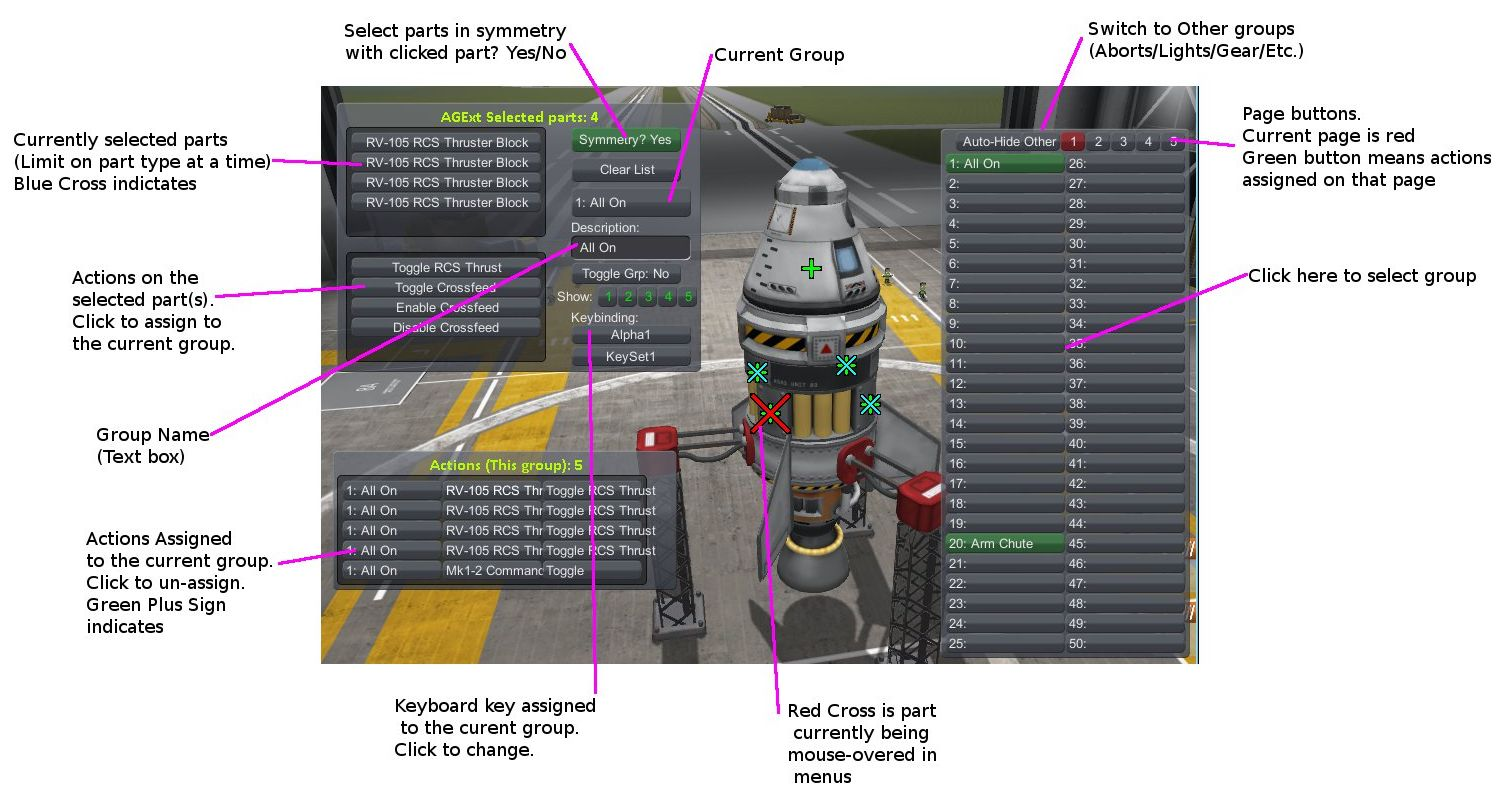
\includegraphics{AGExtQuickStart1.jpg}
\end{figure}
\begin{figure}[htbp]
\centering

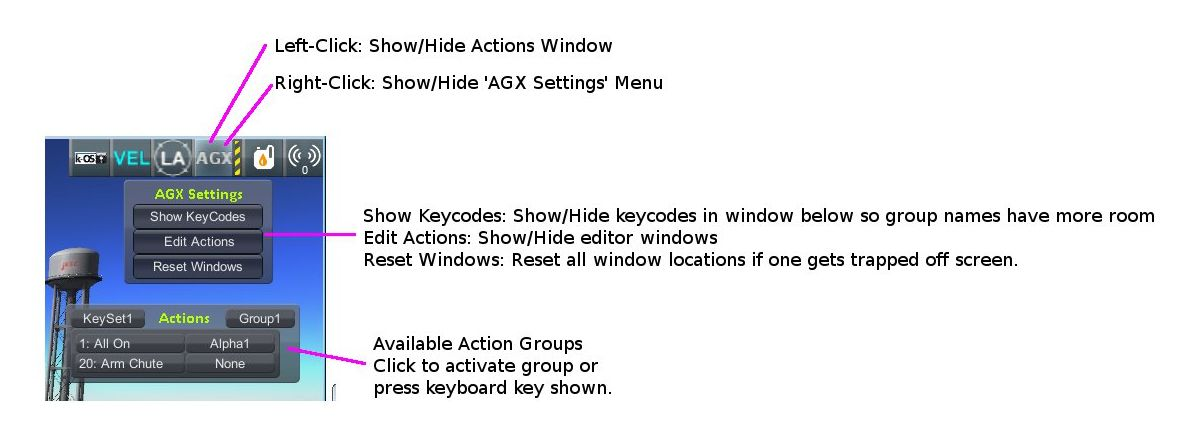
\includegraphics{AGExtQuickStart2.jpg}
\end{figure}

Note that this mod only adds action groups 11 through 250, it does not change how action groups 1 through 10 behave in any way and groups 11 through 250 should behave the same way.

\textbf{Known limitations (Action groups 11 through 250 only):}
\begin{itemize}
\item {} 
On a nearby vessel that is not your current focus, an action group with no actions assigned will always return a state of False and can not be set to a state of true via the ``AG15 on.'' command. Assign the Script Trigger action as a work-around for this.

\item {} 
At this point, AG11 through AG250 do not officially support RemoteTech through kOS. (Support will happen once all three mods involved have updated to KSP version 1.0 and made any internal changes necessary.) All three mods can be installed at the same time without issue, just be aware there may be unexpected behaviour when using action groups 11 through 250 from a kOS script in terms of RemoteTech signal delay and connection state.

\end{itemize}

\textbf{Action state monitoring}

Note that the state of action groups is tracked on a per-action basis, rather then on a per-group basis. This results in the group state being handled differently.
\begin{itemize}
\item {} 
The Script Trigger action found on the kOS computer module is not subject to the below considerations and is the recommended action to use when interacting with a running kOS script.

\item {} 
The state of actions are monitored on the part and updated automatically. A closed solar panel will return a state of false for all it's actions. (Extend Panels, Retract Panels, Toggle Panels) When you extend the solar panel with either the Extend Panels or Toggle Panels action, all three actions will change to a state of True. Retract the panels and the state of all three actions will become False. Note that this state will update in any action group that contains that action, not just the action group that was activated.

\item {} 
This can result in an action group have actions in a mixed state where some actions are on and some are off. In this case querying the group state will result in a state of False. For the purposes of the group state being True or False, if \emph{all} actions in the action group are true, the group state will return true. If \emph{any} actions in the group are false,the group state with return False.

\item {} 
When an action triggers an animation, the state of the action will be uncertain until the animation finishes playing. Some parts will report True during the animation and some will report False. It depends on how the part creator set things up and not something AGX can control.

\item {} 
For clarity, visual feedback can be provided of the current state of an action group. When editing action groups, find the ``Toggle Grp.'' button just below the text entry field for the group name in the main AGX window and enable it. (It is enabled/disabled for the current action group when you click the button.) Once you do this, the text displaying that group will change from gray to colored. Green: Group is activated (state True). Red: Group is deactivated (state False). Yellow: Group is in a mixed state, will return a state False when queried.

\item {} 
It is okay to activate an already activated group and deactivate a non-activated group. Actions in the group will still try to execute as normal. Exact behaviour of a specific action will depend on how the action's creator set things up.

\end{itemize}

\textbf{Example code:}

Print to the terminal any time you activate action group 15. Use this to change variables within a running kOS script and the ``Script Trigger'' action found on the kOS computer part:

\begin{Verbatim}[commandchars=\\\{\}]
\PYG{n}{AG15} \PYG{n}{on}\PYG{p}{.} \PYG{c+c1}{// Activate action group 15.}
\PYG{n}{print} \PYG{n}{AG15}\PYG{p}{.} \PYG{c+c1}{// Print action group 15\PYGZsq{}s state to the terminal. (True/False)}

\PYG{n}{on} \PYG{n}{AG15} \PYG{p}{\PYGZob{}} \PYG{c+c1}{//Prints \PYGZdq{}Action group 15 clicked!\PYGZdq{} to the console when AG15 is toggled, either via \PYGZdq{}AG15 on.\PYGZdq{} or in\PYGZhy{}game with an assigned key.}
  \PYG{n}{print} \PYG{l+s}{\PYGZdq{}}\PYG{l+s}{Action group 15 clicked!}\PYG{l+s}{\PYGZdq{}}\PYG{p}{.}
  \PYG{n}{preserve}\PYG{p}{.}
\PYG{p}{\PYGZcb{}}
\end{Verbatim}

\textbf{Animation Delay:}
\begin{itemize}
\item {} 
Using the above code on a stock solar panel's Toggle Panels action, the player activates AG15, AG15's state goes from false to true and the actions are triggered. \code{AG15 False -\textgreater{} True} and prints to the terminal.

\item {} 
On it's next update pass (100ms to 250ms later), AGX checks AG15's state and sees the solar panel is still deploying which means that AG15's state is false and so sets it that way. \code{AG15 True -\textgreater{} False} and prints to the terminal.

\item {} 
A few seconds later, the solar panel finishes it's deployment animation. On it's next update pass AGX checks AG15's state and sees the solar panel is now deployed which means that AG15's state is now true and so sets it that way. \code{AG15 False -\textgreater{} True} and prints to the terminal a third time.

\end{itemize}

As a workaround, you need to add a cooldown:

\begin{Verbatim}[commandchars=\\\{\}]
\PYG{n}{declare} \PYG{n}{cooldownTimeAG15} \PYG{n}{to} \PYG{l+m+mf}{0.}
\PYG{n}{on} \PYG{n}{AG15} \PYG{p}{\PYGZob{}}
  \PYG{k}{if} \PYG{n}{cooldownTimeAG15} \PYG{o}{+} \PYG{l+m+mi}{10} \PYG{o}{\PYGZlt{}} \PYG{n+nl}{time}\PYG{p}{:}\PYG{n}{seconds} \PYG{p}{\PYGZob{}}
    \PYG{n}{print} \PYG{l+s}{\PYGZdq{}}\PYG{l+s}{Solar Panel Toggled!}\PYG{l+s}{\PYGZdq{}}\PYG{p}{.}
    \PYG{n}{set} \PYG{n}{cooldownTimeAG15} \PYG{n}{to} \PYG{n}{time}\PYG{p}{.}
  \PYG{p}{\PYGZcb{}}
  \PYG{n}{preserve}\PYG{p}{.}
\PYG{p}{\PYGZcb{}}
\end{Verbatim}

Note the 10 in the second line, that is your cooldown time in seconds. Set this to a number of seconds that is longer then your animation time and the above code will limit whatever is inside the IF statement so it can only activate after 10 seconds have passed since the previous activation and will not try to activate a second time while the solar panel animation is still playing.


\section{RemoteTech}
\label{addons/RemoteTech:remotetech}\label{addons/RemoteTech::doc}\label{addons/RemoteTech:id1}
RemoteTech is a modification for Squad’s ``Kerbal Space Program'' (KSP) which overhauls the unmanned space program. It does this by requiring unmanned vessels have a connection to Kerbal Space Center (KSC) to be able to be controlled. This adds a new layer of difficulty that compensates for the lack of live crew members.
\begin{itemize}
\item {} 
Download: \href{http://kerbalstuff.com/mod/134/RemoteTech}{http://kerbalstuff.com/mod/134/RemoteTech}

\item {} 
Sources: \href{https://github.com/RemoteTechnologiesGroup/RemoteTech}{https://github.com/RemoteTechnologiesGroup/RemoteTech}

\item {} 
Documentation: \href{http://remotetechnologiesgroup.github.io/RemoteTech/}{http://remotetechnologiesgroup.github.io/RemoteTech/}

\end{itemize}


\subsection{Interaction with kOS}
\label{addons/RemoteTech:interaction-with-kos}
When you have RemoteTech installed you can only interact with the core's terminal when you have a connection to KSC on any unmanned craft. Scripts launched when you still had a connection will continue to execute even if your unmanned craft loses connection to KSC. But you should note, that when there is no connection to KSC the archive volume is inaccessible. This will require you to plan ahead and copy necessary scripts for your mission to probe hard disk, if your kerbals and/or other scripts need to use them while not connected.

If you launch a manned craft while using RemoteTech, you are still able to input commands from the terminal even if you do not have a connection to the KSC.  The archive will still be inaccessible without a connection to the KSC.  Under the current implementation, there is no delay when accessing the archive with a local terminal.  This implementation may change in the future to account for delays in reading and writing data over the connection.

It is possible to activate/deactivate RT antennas, as well as set their targets using kOS:

\begin{Verbatim}[commandchars=\\\{\}]
\PYG{n}{SET} \PYG{n}{p} \PYG{n}{TO} \PYG{n+nl}{SHIP}\PYG{p}{:}\PYG{n}{PARTSNAMED}\PYG{p}{(}\PYG{l+s}{\PYGZdq{}}\PYG{l+s}{mediumDishAntenna}\PYG{l+s}{\PYGZdq{}}\PYG{p}{)}\PYG{p}{[}\PYG{l+m+mi}{0}\PYG{p}{]}\PYG{p}{.}
\PYG{n}{SET} \PYG{n}{m} \PYG{n}{to} \PYG{n+nl}{p}\PYG{p}{:}\PYG{n}{GETMODULE}\PYG{p}{(}\PYG{l+s}{\PYGZdq{}}\PYG{l+s}{ModuleRTAntenna}\PYG{l+s}{\PYGZdq{}}\PYG{p}{)}\PYG{p}{.}
\PYG{n+nl}{m}\PYG{p}{:}\PYG{n}{DOEVENT}\PYG{p}{(}\PYG{l+s}{\PYGZdq{}}\PYG{l+s}{activate}\PYG{l+s}{\PYGZdq{}}\PYG{p}{)}\PYG{p}{.}
\PYG{n+nl}{m}\PYG{p}{:}\PYG{n}{SETFIELD}\PYG{p}{(}\PYG{l+s}{\PYGZdq{}}\PYG{l+s}{target}\PYG{l+s}{\PYGZdq{}}\PYG{p}{,} \PYG{l+s}{\PYGZdq{}}\PYG{l+s}{mission\PYGZhy{}control}\PYG{l+s}{\PYGZdq{}}\PYG{p}{)}\PYG{p}{.}
\PYG{c+c1}{// or}
\PYG{n+nl}{m}\PYG{p}{:}\PYG{n}{SETFIELD}\PYG{p}{(}\PYG{l+s}{\PYGZdq{}}\PYG{l+s}{target}\PYG{l+s}{\PYGZdq{}}\PYG{p}{,} \PYG{n}{mun}\PYG{p}{)}\PYG{p}{.}
\PYG{n+nl}{m}\PYG{p}{:}\PYG{n}{SETFIELD}\PYG{p}{(}\PYG{l+s}{\PYGZdq{}}\PYG{l+s}{target}\PYG{l+s}{\PYGZdq{}}\PYG{p}{,} \PYG{l+s}{\PYGZdq{}}\PYG{l+s}{minmus}\PYG{l+s}{\PYGZdq{}}\PYG{p}{)}\PYG{p}{.}
\end{Verbatim}

Acceptable values for \emph{``target''} are: \emph{``no-target''}, \emph{``active-vessel''}, \emph{``mission-control''}, a {\hyperref[structures/celestial_bodies/body:structure:BODY]{\emph{\code{Body}}}}, a {\hyperref[structures/vessels/vessel:structure:VESSEL]{\emph{\code{Vessel}}}}, or a string containing the name of a body or vessel.

Starting version 0.17 of kOS you can access structure RTAddon via \emph{ADDONS:RT}.
\index{RTAddon {[}struct{]}}

\begin{fulllineitems}
\phantomsection\label{addons/RemoteTech:structure:RTADDON}\pysigline{\strong{structure }\bfcode{RTAddon}}~
\begin{tabulary}{\linewidth}{|L|L|L|}
\hline
\textsf{\relax 
Suffix
} & \textsf{\relax 
Type
} & \textsf{\relax 
Description
}\\
\hline
{\hyperref[addons/RemoteTech:attribute:RTADDON:AVAILABLE]{\emph{\code{AVAILABLE}}}}
 & 
bool(readonly)
 & 
True if RT is installed and RT integration enabled.
\\
\hline
{\hyperref[addons/RemoteTech:method:RTADDON:DELAY]{\emph{\code{DELAY(vessel)}}}}
 & 
double
 & 
Get shortest possible delay to given {\hyperref[structures/vessels/vessel:structure:VESSEL]{\emph{\code{Vessel}}}}
\\
\hline
{\hyperref[addons/RemoteTech:method:RTADDON:KSCDELAY]{\emph{\code{KSCDELAY(vessel)}}}}
 & 
double
 & 
Get delay from KSC to given {\hyperref[structures/vessels/vessel:structure:VESSEL]{\emph{\code{Vessel}}}}
\\
\hline
{\hyperref[addons/RemoteTech:method:RTADDON:HASCONNECTION]{\emph{\code{HASCONNECTION(vessel)}}}}
 & 
bool
 & 
True if given {\hyperref[structures/vessels/vessel:structure:VESSEL]{\emph{\code{Vessel}}}} has any connection
\\
\hline
{\hyperref[addons/RemoteTech:method:RTADDON:HASKSCCONNECTION]{\emph{\code{HASKSCCONNECTION(vessel)}}}}
 & 
bool
 & 
True if given {\hyperref[structures/vessels/vessel:structure:VESSEL]{\emph{\code{Vessel}}}} has connection to KSC
\\
\hline
{\hyperref[addons/RemoteTech:method:RTADDON:HASLOCALCONTROL]{\emph{\code{HASLOCALCONTROL(vessel)}}}}
 & 
bool
 & 
True if given {\hyperref[structures/vessels/vessel:structure:VESSEL]{\emph{\code{Vessel}}}} has local control
\\
\hline\end{tabulary}


\end{fulllineitems}

\index{RTADDON:AVAILABLE}

\begin{fulllineitems}
\phantomsection\label{addons/RemoteTech:attribute:RTADDON:AVAILABLE}\pysigline{RTADDON:\bfcode{AVAILABLE}}~\begin{quote}\begin{description}
\item[{Type}] \leavevmode
bool

\item[{Access}] \leavevmode
Get only

\end{description}\end{quote}

True if RT is installed and RT integration enabled.

\end{fulllineitems}

\index{RTAddon:DELAY()}

\begin{fulllineitems}
\phantomsection\label{addons/RemoteTech:method:RTADDON:DELAY}\pysiglinewithargsret{RTAddon:\bfcode{DELAY}}{vessel}{}~\begin{quote}\begin{description}
\item[{Parameters}] \leavevmode\begin{itemize}
\item {} 
\textbf{\texttt{vessel}} -- {\hyperref[structures/vessels/vessel:structure:VESSEL]{\emph{\code{Vessel}}}}

\end{itemize}

\item[{Returns}] \leavevmode
(double) seconds

\end{description}\end{quote}

Returns shortest possible delay for \emph{vessel} (Will be less than KSC delay if you have a local command post).

\end{fulllineitems}

\index{RTAddon:KSCDELAY()}

\begin{fulllineitems}
\phantomsection\label{addons/RemoteTech:method:RTADDON:KSCDELAY}\pysiglinewithargsret{RTAddon:\bfcode{KSCDELAY}}{vessel}{}~\begin{quote}\begin{description}
\item[{Parameters}] \leavevmode\begin{itemize}
\item {} 
\textbf{\texttt{vessel}} -- {\hyperref[structures/vessels/vessel:structure:VESSEL]{\emph{\code{Vessel}}}}

\end{itemize}

\item[{Returns}] \leavevmode
(double) seconds

\end{description}\end{quote}

Returns delay in seconds from KSC to \emph{vessel}.

\end{fulllineitems}

\index{RTAddon:HASCONNECTION()}

\begin{fulllineitems}
\phantomsection\label{addons/RemoteTech:method:RTADDON:HASCONNECTION}\pysiglinewithargsret{RTAddon:\bfcode{HASCONNECTION}}{vessel}{}~\begin{quote}\begin{description}
\item[{Parameters}] \leavevmode\begin{itemize}
\item {} 
\textbf{\texttt{vessel}} -- {\hyperref[structures/vessels/vessel:structure:VESSEL]{\emph{\code{Vessel}}}}

\end{itemize}

\item[{Returns}] \leavevmode
bool

\end{description}\end{quote}

Returns True if \emph{vessel} has any connection (including to local command posts).

\end{fulllineitems}

\index{RTAddon:HASKSCCONNECTION()}

\begin{fulllineitems}
\phantomsection\label{addons/RemoteTech:method:RTADDON:HASKSCCONNECTION}\pysiglinewithargsret{RTAddon:\bfcode{HASKSCCONNECTION}}{vessel}{}~\begin{quote}\begin{description}
\item[{Parameters}] \leavevmode\begin{itemize}
\item {} 
\textbf{\texttt{vessel}} -- {\hyperref[structures/vessels/vessel:structure:VESSEL]{\emph{\code{Vessel}}}}

\end{itemize}

\item[{Returns}] \leavevmode
bool

\end{description}\end{quote}

Returns True if \emph{vessel} has connection to KSC.

\end{fulllineitems}

\index{RTAddon:HASLOCALCONTROL()}

\begin{fulllineitems}
\phantomsection\label{addons/RemoteTech:method:RTADDON:HASLOCALCONTROL}\pysiglinewithargsret{RTAddon:\bfcode{HASLOCALCONTROL}}{vessel}{}~\begin{quote}\begin{description}
\item[{Parameters}] \leavevmode\begin{itemize}
\item {} 
\textbf{\texttt{vessel}} -- {\hyperref[structures/vessels/vessel:structure:VESSEL]{\emph{\code{Vessel}}}}

\end{itemize}

\item[{Returns}] \leavevmode
bool

\end{description}\end{quote}

Returns True if \emph{vessel} has local control (and thus not requiring a RemoteTech connection).

\end{fulllineitems}



\section{Kerbal Alarm Clock}
\label{addons/KAC:kac}\label{addons/KAC:kerbal-alarm-clock}\label{addons/KAC::doc}\begin{itemize}
\item {} 
Download: \href{https://github.com/TriggerAu/KerbalAlarmClock/releases}{https://github.com/TriggerAu/KerbalAlarmClock/releases}

\item {} 
Alternative download \href{https://kerbalstuff.com/mod/231/Kerbal\%20Alarm\%20Clock}{https://kerbalstuff.com/mod/231/Kerbal\%20Alarm\%20Clock}

\item {} 
Forum thread, including full instructions: \href{http://forum.kerbalspaceprogram.com/threads/24786}{http://forum.kerbalspaceprogram.com/threads/24786}

\end{itemize}

The Kerbal Alarm Clock is a plugin that allows you to create reminder alarms at future periods to help you manage your flights and not warp past important times.
\begin{figure}[htbp]
\centering
\end{figure}

Creator of the KAC provides API for integration with other mods. In KOS we provide limited access to KAC alarms via following structure and functions.

Access structure KACAddon via \emph{ADDONS:KAC}.
\index{KACAddon {[}struct{]}}

\begin{fulllineitems}
\phantomsection\label{addons/KAC:structure:KACADDON}\pysigline{\strong{structure }\bfcode{KACAddon}}~
\begin{tabulary}{\linewidth}{|L|L|L|}
\hline
\textsf{\relax 
Suffix
} & \textsf{\relax 
Type
} & \textsf{\relax 
Description
}\\
\hline
{\hyperref[addons/KAC:attribute:KACADDON:AVAILABLE]{\emph{\code{AVAILABLE}}}}
 & 
bool(readonly)
 & 
True if KAC is installed and KAC integration enabled.
\\
\hline
{\hyperref[addons/KAC:method:KACADDON:ALARMS]{\emph{\code{ALARMS()}}}}
 & 
List
 & 
List all alarms
\\
\hline\end{tabulary}


\end{fulllineitems}

\index{KACAddon:AVAILABLE}

\begin{fulllineitems}
\phantomsection\label{addons/KAC:attribute:KACADDON:AVAILABLE}\pysigline{KACAddon:\bfcode{AVAILABLE}}~\begin{quote}\begin{description}
\item[{Type}] \leavevmode
bool

\item[{Access}] \leavevmode
Get only

\end{description}\end{quote}

True if KAC is installed and KAC integration enabled.
Example of use:

\begin{Verbatim}[commandchars=\\\{\}]
\PYG{k}{if} \PYG{n+nl}{ADDONS}\PYG{p}{:}\PYG{n+nl}{KAC}\PYG{p}{:}\PYG{n}{AVAILABLE}
\PYG{p}{\PYGZob{}}
    \PYG{c+c1}{//some KAC dependent code}
\PYG{p}{\PYGZcb{}}
\end{Verbatim}

\end{fulllineitems}

\index{KACAddon:ALARMS()}

\begin{fulllineitems}
\phantomsection\label{addons/KAC:method:KACADDON:ALARMS}\pysiglinewithargsret{KACAddon:\bfcode{ALARMS}}{}{}~\begin{quote}\begin{description}
\item[{Returns}] \leavevmode
List of {\hyperref[addons/KAC:structure:KACALARM]{\emph{\code{KACAlarm}}}} objects

\end{description}\end{quote}

List \textbf{all} the alarms set up in Kerbal Alarm Clock. Example of use:

\begin{Verbatim}[commandchars=\\\{\}]
\PYG{k}{for} \PYG{n}{i} \PYG{n}{in} \PYG{n+nl}{ADDONS}\PYG{p}{:}\PYG{n+nl}{KAC}\PYG{p}{:}\PYG{n}{ALARMS}
\PYG{p}{\PYGZob{}}
        \PYG{n}{print} \PYG{n+nl}{i}\PYG{p}{:}\PYG{n}{NAME} \PYG{o}{+} \PYG{l+s}{\PYGZdq{}}\PYG{l+s}{ \PYGZhy{} }\PYG{l+s}{\PYGZdq{}} \PYG{o}{+} \PYG{n+nl}{i}\PYG{p}{:}\PYG{n}{REMAINING} \PYG{o}{+} \PYG{l+s}{\PYGZdq{}}\PYG{l+s}{ \PYGZhy{} }\PYG{l+s}{\PYGZdq{}} \PYG{o}{+} \PYG{n+nl}{i}\PYG{p}{:}\PYG{n}{TYPE}\PYG{o}{+} \PYG{l+s}{\PYGZdq{}}\PYG{l+s}{ \PYGZhy{} }\PYG{l+s}{\PYGZdq{}} \PYG{o}{+} \PYG{n+nl}{i}\PYG{p}{:}\PYG{n}{ACTION}\PYG{p}{.}
\PYG{p}{\PYGZcb{}}
\end{Verbatim}

\end{fulllineitems}

\index{KACAlarm {[}struct{]}}

\begin{fulllineitems}
\phantomsection\label{addons/KAC:structure:KACALARM}\pysigline{\strong{structure }\bfcode{KACAlarm}}~
\begin{tabulary}{\linewidth}{|L|L|L|}
\hline
\textsf{\relax 
Suffix
} & \textsf{\relax 
Type
} & \textsf{\relax 
Description
}\\
\hline
{\hyperref[addons/KAC:attribute:KACALARM:ID]{\emph{\code{ID}}}}
 & 
string (readonly)
 & 
Unique identifier
\\
\hline
{\hyperref[addons/KAC:attribute:KACALARM:NAME]{\emph{\code{NAME}}}}
 & 
string
 & 
Name of the alarm
\\
\hline
{\hyperref[addons/KAC:attribute:KACALARM:ACTION]{\emph{\code{ACTION}}}}
 & 
string
 & 
What should the Alarm Clock do when the alarm fires
\\
\hline
{\hyperref[addons/KAC:attribute:KACALARM:TYPE]{\emph{\code{TYPE}}}}
 & 
string (readonly)
 & 
What type of Alarm is this - affects icon displayed and some calc options
\\
\hline
{\hyperref[addons/KAC:attribute:KACALARM:NOTES]{\emph{\code{NOTES}}}}
 & 
string
 & 
Long description of the alarm (optional)
\\
\hline
{\hyperref[addons/KAC:attribute:KACALARM:REMAINING]{\emph{\code{REMAINING}}}}
 & 
scalar (s)
 & 
Time remaining until alarm is triggered
\\
\hline
{\hyperref[addons/KAC:attribute:KACALARM:REPEAT]{\emph{\code{REPEAT}}}}
 & 
bool
 & 
Should the alarm be repeated once it fires
\\
\hline
{\hyperref[addons/KAC:attribute:KACALARM:REPEATPERIOD]{\emph{\code{REPEATPERIOD}}}}
 & 
scalar (s)
 & 
How long after the alarm fires should the next alarm be set up
\\
\hline
{\hyperref[addons/KAC:attribute:KACALARM:ORIGINBODY]{\emph{\code{ORIGINBODY}}}}
 & 
string
 & 
Name of the body the vessel is departing from
\\
\hline
{\hyperref[addons/KAC:attribute:KACALARM:TARGETBODY]{\emph{\code{TARGETBODY}}}}
 & 
string
 & 
Name of the body the vessel is arriving at
\\
\hline\end{tabulary}


\end{fulllineitems}

\index{KACAlarm:ID}

\begin{fulllineitems}
\phantomsection\label{addons/KAC:attribute:KACALARM:ID}\pysigline{KACAlarm:\bfcode{ID}}~\begin{quote}\begin{description}
\item[{Type}] \leavevmode
string

\item[{Access}] \leavevmode
Get only

\end{description}\end{quote}

Unique identifier of the alarm.

\end{fulllineitems}

\index{KACAlarm:NAME}

\begin{fulllineitems}
\phantomsection\label{addons/KAC:attribute:KACALARM:NAME}\pysigline{KACAlarm:\bfcode{NAME}}~\begin{quote}\begin{description}
\item[{Type}] \leavevmode
string

\item[{Access}] \leavevmode
Get/Set

\end{description}\end{quote}

Name of the alarm. Displayed in main KAC window.

\end{fulllineitems}

\index{KACAlarm:ACTION}

\begin{fulllineitems}
\phantomsection\label{addons/KAC:attribute:KACALARM:ACTION}\pysigline{KACAlarm:\bfcode{ACTION}}~\begin{quote}\begin{description}
\item[{Type}] \leavevmode
string

\item[{Access}] \leavevmode
Get/Set

\end{description}\end{quote}

Should be one of the following
\begin{itemize}
\item {} 
\emph{MessageOnly} - Message Only-No Affect on warp

\item {} 
\emph{KillWarpOnly} - Kill Warp Only-No Message

\item {} 
\emph{KillWarp} - Kill Warp and Message

\item {} 
\emph{PauseGame} - Pause Game and Message

\end{itemize}

If set incorrectly will log a warning in Debug log and revert to previous or default value.

\end{fulllineitems}

\index{KACAlarm:TYPE}

\begin{fulllineitems}
\phantomsection\label{addons/KAC:attribute:KACALARM:TYPE}\pysigline{KACAlarm:\bfcode{TYPE}}~\begin{quote}\begin{description}
\item[{Type}] \leavevmode
string

\item[{Access}] \leavevmode
Get only

\end{description}\end{quote}

Can only be set at Alarm creation.
Could be one of the following as per API
\begin{itemize}
\item {} 
Raw (default)

\item {} 
Maneuver

\item {} 
ManeuverAuto

\item {} 
Apoapsis

\item {} 
Periapsis

\item {} 
AscendingNode

\item {} 
DescendingNode

\item {} 
LaunchRendevous

\item {} 
Closest

\item {} 
SOIChange

\item {} 
SOIChangeAuto

\item {} 
Transfer

\item {} 
TransferModelled

\item {} 
Distance

\item {} 
Crew

\item {} 
EarthTime

\end{itemize}

\textbf{Warning}: Unless you are 100\% certain you know what you're doing, create only ``Raw'' AlarmTypes to avoid unnecessary complications.

\end{fulllineitems}

\index{KACAlarm:NOTES}

\begin{fulllineitems}
\phantomsection\label{addons/KAC:attribute:KACALARM:NOTES}\pysigline{KACAlarm:\bfcode{NOTES}}~\begin{quote}\begin{description}
\item[{Type}] \leavevmode
string

\item[{Access}] \leavevmode
Get/Set

\end{description}\end{quote}

Long description of the alarm. Can be seen when alarm pops or by double-clicking alarm in UI.

\textbf{Warning}: This field may be reserved in the future version of KAC-KOS integration for automated script execution upon triggering of the alarm.

\end{fulllineitems}

\index{KACAlarm:REMAINING}

\begin{fulllineitems}
\phantomsection\label{addons/KAC:attribute:KACALARM:REMAINING}\pysigline{KACAlarm:\bfcode{REMAINING}}~\begin{quote}\begin{description}
\item[{Type}] \leavevmode
double

\item[{Access}] \leavevmode
Get only

\end{description}\end{quote}

Time remaining until alarm is triggered.

\end{fulllineitems}

\index{KACAlarm:REPEAT}

\begin{fulllineitems}
\phantomsection\label{addons/KAC:attribute:KACALARM:REPEAT}\pysigline{KACAlarm:\bfcode{REPEAT}}~\begin{quote}\begin{description}
\item[{Type}] \leavevmode
bool

\item[{Access}] \leavevmode
Get/Set

\end{description}\end{quote}

Should the alarm be repeated once it fires.

\end{fulllineitems}

\index{KACAlarm:REPEATPERIOD}

\begin{fulllineitems}
\phantomsection\label{addons/KAC:attribute:KACALARM:REPEATPERIOD}\pysigline{KACAlarm:\bfcode{REPEATPERIOD}}~\begin{quote}\begin{description}
\item[{Type}] \leavevmode
double

\item[{Access}] \leavevmode
Get/Set

\end{description}\end{quote}

How long after the alarm fires should the next alarm be set up.

\end{fulllineitems}

\index{KACAlarm:ORIGINBODY}

\begin{fulllineitems}
\phantomsection\label{addons/KAC:attribute:KACALARM:ORIGINBODY}\pysigline{KACAlarm:\bfcode{ORIGINBODY}}~\begin{quote}\begin{description}
\item[{Type}] \leavevmode
string

\item[{Access}] \leavevmode
Get/Set

\end{description}\end{quote}

Name of the body the vessel is departing from.

\end{fulllineitems}

\index{KACAlarm:TARGETBODY}

\begin{fulllineitems}
\phantomsection\label{addons/KAC:attribute:KACALARM:TARGETBODY}\pysigline{KACAlarm:\bfcode{TARGETBODY}}~\begin{quote}\begin{description}
\item[{Type}] \leavevmode
string

\item[{Access}] \leavevmode
Get/Set

\end{description}\end{quote}

Name of the body the vessel is arriving to.

\end{fulllineitems}



\subsection{Available Functions}
\label{addons/KAC:available-functions}
\begin{tabulary}{\linewidth}{|L|L|}
\hline
\textsf{\relax 
Function
} & \textsf{\relax 
Description
}\\
\hline
{\hyperref[addons/KAC:function:ADDALARM]{\emph{\code{ADDALARM(AlarmType, UT, Name, Notes)}}}}
 & 
Create new alarm of AlarmType at UT
\\
\hline
{\hyperref[addons/KAC:function:LISTALARMS]{\emph{\code{LISTALARMS(alarmType)}}}}
 & 
List alarms with type \emph{alarmType}.
\\
\hline
{\hyperref[addons/KAC:function:DELETEALARM]{\emph{\code{DELETEALARM(alarmID)}}}}
 & 
Delete alarm with ID = alarmID
\\
\hline\end{tabulary}

\index{ADDALARM()}

\begin{fulllineitems}
\phantomsection\label{addons/KAC:function:ADDALARM}\pysiglinewithargsret{\bfcode{ADDALARM}}{AlarmType, UT, Name, Notes}{}
Creates alarm of type \emph{KACAlarm:ALARMTYPE} at \emph{UT} with \emph{Name} and \emph{Notes} attributes set. Attaches alarm to current {\hyperref[general/cpu_vessel:cpu-vessel]{\emph{\DUspan{}{CPU Vessel}}}}.  Returns {\hyperref[addons/KAC:structure:KACALARM]{\emph{\code{KACAlarm}}}} object if creation was successful and empty string otherwise:

\begin{Verbatim}[commandchars=\\\{\}]
\PYG{n}{set} \PYG{n}{na} \PYG{n}{to} \PYG{n}{addAlarm}\PYG{p}{(}\PYG{l+s}{\PYGZdq{}}\PYG{l+s}{Raw}\PYG{l+s}{\PYGZdq{}}\PYG{p}{,}\PYG{n+nl}{time}\PYG{p}{:}\PYG{n}{seconds}\PYG{o}{+}\PYG{l+m+mi}{300}\PYG{p}{,} \PYG{l+s}{\PYGZdq{}}\PYG{l+s}{Test}\PYG{l+s}{\PYGZdq{}}\PYG{p}{,} \PYG{l+s}{\PYGZdq{}}\PYG{l+s}{Notes}\PYG{l+s}{\PYGZdq{}}\PYG{p}{)}\PYG{p}{.}
\PYG{n}{print} \PYG{n+nl}{na}\PYG{p}{:}\PYG{n}{NAME}\PYG{p}{.} \PYG{c+c1}{//prints \PYGZsq{}Test\PYGZsq{}}
\PYG{n}{set} \PYG{n+nl}{na}\PYG{p}{:}\PYG{n}{NOTES} \PYG{n}{to} \PYG{l+s}{\PYGZdq{}}\PYG{l+s}{New Description}\PYG{l+s}{\PYGZdq{}}\PYG{p}{.}
\PYG{n}{print} \PYG{n+nl}{na}\PYG{p}{:}\PYG{n}{NOTES}\PYG{p}{.} \PYG{c+c1}{//prints \PYGZsq{}New Description\PYGZsq{}}
\end{Verbatim}

\end{fulllineitems}

\index{LISTALARMS()}

\begin{fulllineitems}
\phantomsection\label{addons/KAC:function:LISTALARMS}\pysiglinewithargsret{\bfcode{LISTALARMS}}{alarmType}{}
If \emph{alarmType} equals ``All'', returns {\hyperref[structures/misc/list:structure:LIST]{\emph{\code{List}}}} of \emph{all} {\hyperref[addons/KAC:structure:KACALARM]{\emph{\code{KACAlarm}}}} objects attached to current vessel or have no vessel attached.
Otherwise returns {\hyperref[structures/misc/list:structure:LIST]{\emph{\code{List}}}} of all {\hyperref[addons/KAC:structure:KACALARM]{\emph{\code{KACAlarm}}}} objects with \emph{KACAlarm:TYPE} equeal to \emph{alarmType} and attached to current vessel or have no vessel attached.:

\begin{Verbatim}[commandchars=\\\{\}]
\PYG{n}{set} \PYG{n}{al} \PYG{n}{to} \PYG{n}{listAlarms}\PYG{p}{(}\PYG{l+s}{\PYGZdq{}}\PYG{l+s}{All}\PYG{l+s}{\PYGZdq{}}\PYG{p}{)}\PYG{p}{.}
\PYG{k}{for} \PYG{n}{i} \PYG{n}{in} \PYG{n}{al}
\PYG{p}{\PYGZob{}}
    \PYG{n}{print} \PYG{n+nl}{i}\PYG{p}{:}\PYG{n}{ID} \PYG{o}{+} \PYG{l+s}{\PYGZdq{}}\PYG{l+s}{ \PYGZhy{} }\PYG{l+s}{\PYGZdq{}} \PYG{o}{+} \PYG{n+nl}{i}\PYG{p}{:}\PYG{n}{name}\PYG{p}{.}
\PYG{p}{\PYGZcb{}}
\end{Verbatim}

\end{fulllineitems}

\index{DELETEALARM()}

\begin{fulllineitems}
\phantomsection\label{addons/KAC:function:DELETEALARM}\pysiglinewithargsret{\bfcode{DELETEALARM}}{alarmID}{}
Deletes alarm with ID equal to alarmID. Returns True if successful, false otherwise:

\begin{Verbatim}[commandchars=\\\{\}]
\PYG{n}{set} \PYG{n}{na} \PYG{n}{to} \PYG{n+nf}{addAlarm}\PYG{p}{(}\PYG{l+s}{\PYGZdq{}}\PYG{l+s}{Raw}\PYG{l+s}{\PYGZdq{}}\PYG{p}{,}\PYG{n+nl}{time}\PYG{p}{:}\PYG{n}{seconds}\PYG{o}{+}\PYG{l+m+mi}{300}\PYG{p}{,} \PYG{l+s}{\PYGZdq{}}\PYG{l+s}{Test}\PYG{l+s}{\PYGZdq{}}\PYG{p}{,} \PYG{l+s}{\PYGZdq{}}\PYG{l+s}{Notes}\PYG{l+s}{\PYGZdq{}}\PYG{p}{)}\PYG{p}{.}
\PYG{k}{if} \PYG{p}{(}\PYG{n}{DELETEALARM}\PYG{p}{(}\PYG{n+nl}{na}\PYG{p}{:}\PYG{n}{ID}\PYG{p}{)}\PYG{p}{)}
\PYG{p}{\PYGZob{}}
    \PYG{n}{print} \PYG{l+s}{\PYGZdq{}}\PYG{l+s}{Alarm Deleted}\PYG{l+s}{\PYGZdq{}}\PYG{p}{.}
\PYG{p}{\PYGZcb{}}
\end{Verbatim}

\end{fulllineitems}



\section{Infernal Robotics}
\label{addons/IR:infernal-robotics}\label{addons/IR:ir}\label{addons/IR::doc}\begin{itemize}
\item {} 
Download: \href{http://kerbal.curseforge.com/ksp-mods/220267}{http://kerbal.curseforge.com/ksp-mods/220267}

\item {} 
Alternative download: \href{https://kerbalstuff.com/mod/8/Magic\_Smoke\_Industries\_Infernal\_Robotics}{https://kerbalstuff.com/mod/8/Magic\_Smoke\_Industries\_Infernal\_Robotics}

\item {} 
Forum thread, including full instructions: \href{http://forum.kerbalspaceprogram.com/threads/116064}{http://forum.kerbalspaceprogram.com/threads/116064}

\end{itemize}

Infernal Robotics introduces robotics parts to the game, letting you create moving or spinning contraptions that just aren't possible under stock KSP.
.. figure:: \href{http://i.imgur.com/O94LBvF.png}{http://i.imgur.com/O94LBvF.png}

Starting version 0.20 of the Infernal Robotics, mod creators introduced API to for easier access to robotic features.

Access structure IRAddon via \emph{ADDONS:IR}.
\index{IRAddon {[}struct{]}}

\begin{fulllineitems}
\phantomsection\label{addons/IR:structure:IRADDON}\pysigline{\strong{structure }\bfcode{IRAddon}}~
\begin{tabulary}{\linewidth}{|L|L|L|}
\hline
\textsf{\relax 
Suffix
} & \textsf{\relax 
Type
} & \textsf{\relax 
Description
}\\
\hline
{\hyperref[addons/IR:attribute:IRADDON:AVAILABLE]{\emph{\code{AVAILABLE}}}}
 & 
bool(readonly)
 & 
Returns True if mod Infernal Robotics is installed, available to KOS and applicable to current craft.
\\
\hline
{\hyperref[addons/IR:attribute:IRADDON:GROUPS]{\emph{\code{GROUPS}}}}
 & 
List (readonly)
 & 
Lists all Servo Groups for current focused vessel
\\
\hline
{\hyperref[addons/IR:attribute:IRADDON:ALLSERVOS]{\emph{\code{ALLSERVOS}}}}
 & 
List (readonly)
 & 
Lists all Servos for current focused vessel
\\
\hline\end{tabulary}


\end{fulllineitems}

\index{IRAddon:AVAILABLE}

\begin{fulllineitems}
\phantomsection\label{addons/IR:attribute:IRADDON:AVAILABLE}\pysigline{IRAddon:\bfcode{AVAILABLE}}~\begin{quote}\begin{description}
\item[{Type}] \leavevmode
bool

\item[{Access}] \leavevmode
Get only

\end{description}\end{quote}

Returns True if mod Infernal Robotics is installed, available to KOS and applicable to current craft.
Example of use:

\begin{Verbatim}[commandchars=\\\{\}]
\PYG{k}{if} \PYG{n+nl}{ADDONS}\PYG{p}{:}\PYG{n+nl}{IR}\PYG{p}{:}\PYG{n}{AVAILABLE}
\PYG{p}{\PYGZob{}}
    \PYG{c+c1}{//some IR dependent code}
\PYG{p}{\PYGZcb{}}
\end{Verbatim}

\end{fulllineitems}

\index{IRAddon:GROUPS}

\begin{fulllineitems}
\phantomsection\label{addons/IR:attribute:IRADDON:GROUPS}\pysigline{IRAddon:\bfcode{GROUPS}}~\begin{quote}\begin{description}
\item[{Type}] \leavevmode
List of {\hyperref[addons/IR:structure:IRCONTROLGROUP]{\emph{\code{IRControlGroup}}}} objects

\item[{Access}] \leavevmode
Get only

\end{description}\end{quote}

Lists all Servo Groups for current focused vessel. Example of use:

\begin{Verbatim}[commandchars=\\\{\}]
\PYG{k}{for} \PYG{n}{g} \PYG{n}{in} \PYG{n+nl}{ADDONS}\PYG{p}{:}\PYG{n+nl}{IR}\PYG{p}{:}\PYG{n}{GROUPS}
\PYG{p}{\PYGZob{}}
    \PYG{n}{Print} \PYG{n+nl}{g}\PYG{p}{:}\PYG{n}{NAME} \PYG{o}{+} \PYG{l+s}{\PYGZdq{}}\PYG{l+s}{ contains }\PYG{l+s}{\PYGZdq{}} \PYG{o}{+} \PYG{n+nl}{g}\PYG{p}{:}\PYG{n+nl}{SERVOS}\PYG{p}{:}\PYG{n}{LENGTH} \PYG{o}{+} \PYG{l+s}{\PYGZdq{}}\PYG{l+s}{ servos}\PYG{l+s}{\PYGZdq{}}\PYG{p}{.}
\PYG{p}{\PYGZcb{}}
\end{Verbatim}

\end{fulllineitems}

\index{IRAddon:ALLSERVOS}

\begin{fulllineitems}
\phantomsection\label{addons/IR:attribute:IRADDON:ALLSERVOS}\pysigline{IRAddon:\bfcode{ALLSERVOS}}~\begin{quote}\begin{description}
\item[{Type}] \leavevmode
List of {\hyperref[addons/IR:structure:IRSERVO]{\emph{\code{IRServo}}}} objects

\item[{Access}] \leavevmode
Get only

\end{description}\end{quote}

Lists all Servos for current focused vessel. Example of use:

\begin{Verbatim}[commandchars=\\\{\}]
\PYG{k}{for} \PYG{n}{s} \PYG{n}{in} \PYG{n+nl}{ADDONS}\PYG{p}{:}\PYG{n+nl}{IR}\PYG{p}{:}\PYG{n}{ALLSERVOS}
\PYG{p}{\PYGZob{}}
    \PYG{n}{print} \PYG{l+s}{\PYGZdq{}}\PYG{l+s}{Name: }\PYG{l+s}{\PYGZdq{}} \PYG{o}{+} \PYG{n+nl}{s}\PYG{p}{:}\PYG{n}{NAME} \PYG{o}{+} \PYG{l+s}{\PYGZdq{}}\PYG{l+s}{, position: }\PYG{l+s}{\PYGZdq{}} \PYG{o}{+} \PYG{n+nl}{s}\PYG{p}{:}\PYG{n}{POSITION}\PYG{p}{.}
\PYG{p}{\PYGZcb{}}
\end{Verbatim}

\end{fulllineitems}

\index{IRControlGroup {[}struct{]}}

\begin{fulllineitems}
\phantomsection\label{addons/IR:structure:IRCONTROLGROUP}\pysigline{\strong{structure }\bfcode{IRControlGroup}}~
\begin{tabulary}{\linewidth}{|L|L|L|}
\hline
\textsf{\relax 
Suffix
} & \textsf{\relax 
Type
} & \textsf{\relax 
Description
}\\
\hline
{\hyperref[addons/IR:attribute:IRCONTROLGROUP:NAME]{\emph{\code{NAME}}}}
 & 
string
 & 
Name of the Control Group
\\
\hline
{\hyperref[addons/IR:attribute:IRCONTROLGROUP:SPEED]{\emph{\code{SPEED}}}}
 & 
float
 & 
Speed multiplier set in the IR UI
\\
\hline
{\hyperref[addons/IR:attribute:IRCONTROLGROUP:EXPANDED]{\emph{\code{EXPANDED}}}}
 & 
bool
 & 
True if Group is expanded in IR UI
\\
\hline
{\hyperref[addons/IR:attribute:IRCONTROLGROUP:FORWARDKEY]{\emph{\code{FORWARDKEY}}}}
 & 
string
 & 
Key assigned to forward movement
\\
\hline
{\hyperref[addons/IR:attribute:IRCONTROLGROUP:REVERSEKEY]{\emph{\code{REVERSEKEY}}}}
 & 
string
 & 
Key assigned to reverse movement
\\
\hline
{\hyperref[addons/IR:attribute:IRCONTROLGROUP:SERVOS]{\emph{\code{SERVOS}}}}
 & 
List (readonly)
 & 
List of servos in the group
\\
\hline
{\hyperref[addons/IR:method:IRCONTROLGROUP:MOVERIGHT]{\emph{\code{MOVERIGHT()}}}}
 & 
void
 & 
Commands servos in the group to move in positive direction
\\
\hline
{\hyperref[addons/IR:method:IRCONTROLGROUP:MOVELEFT]{\emph{\code{MOVELEFT()}}}}
 & 
void
 & 
Commands servos in the group to move in negative direction
\\
\hline
{\hyperref[addons/IR:method:IRCONTROLGROUP:MOVECENTER]{\emph{\code{MOVECENTER()}}}}
 & 
void
 & 
Commands servos in the group to move to default position
\\
\hline
{\hyperref[addons/IR:method:IRCONTROLGROUP:MOVENEXTPRESET]{\emph{\code{MOVENEXTPRESET()}}}}
 & 
void
 & 
Commands servos in the group to move to next preset
\\
\hline
{\hyperref[addons/IR:method:IRCONTROLGROUP:MOVEPREVPRESET]{\emph{\code{MOVEPREVPRESET()}}}}
 & 
void
 & 
Commands servos in the group to move to previous preset
\\
\hline
{\hyperref[addons/IR:method:IRCONTROLGROUP:STOP]{\emph{\code{STOP()}}}}
 & 
void
 & 
Commands servos in the group to stop
\\
\hline\end{tabulary}


\end{fulllineitems}

\index{IRControlGroup:NAME}

\begin{fulllineitems}
\phantomsection\label{addons/IR:attribute:IRCONTROLGROUP:NAME}\pysigline{IRControlGroup:\bfcode{NAME}}~\begin{quote}\begin{description}
\item[{Type}] \leavevmode
string

\item[{Access}] \leavevmode
Get/Set

\end{description}\end{quote}

Name of the Control Group (cannot be empty).

\end{fulllineitems}

\index{IRControlGroup:SPEED}

\begin{fulllineitems}
\phantomsection\label{addons/IR:attribute:IRCONTROLGROUP:SPEED}\pysigline{IRControlGroup:\bfcode{SPEED}}~\begin{quote}\begin{description}
\item[{Type}] \leavevmode
float

\item[{Access}] \leavevmode
Get/Set

\end{description}\end{quote}

Speed multiplier as set in the IR user interface. Avoid setting it to 0.

\end{fulllineitems}

\index{IRControlGroup:EXPANDED}

\begin{fulllineitems}
\phantomsection\label{addons/IR:attribute:IRCONTROLGROUP:EXPANDED}\pysigline{IRControlGroup:\bfcode{EXPANDED}}~\begin{quote}\begin{description}
\item[{Type}] \leavevmode
bool

\item[{Access}] \leavevmode
Get/Set

\end{description}\end{quote}

True if Group is expanded in IR UI

\end{fulllineitems}

\index{IRControlGroup:FORWARDKEY}

\begin{fulllineitems}
\phantomsection\label{addons/IR:attribute:IRCONTROLGROUP:FORWARDKEY}\pysigline{IRControlGroup:\bfcode{FORWARDKEY}}~\begin{quote}\begin{description}
\item[{Type}] \leavevmode
string

\item[{Access}] \leavevmode
Get/Set

\end{description}\end{quote}

Key assigned to forward movement. Can be empty.

\end{fulllineitems}

\index{IRControlGroup:REVERSEKEY}

\begin{fulllineitems}
\phantomsection\label{addons/IR:attribute:IRCONTROLGROUP:REVERSEKEY}\pysigline{IRControlGroup:\bfcode{REVERSEKEY}}~\begin{quote}\begin{description}
\item[{Type}] \leavevmode
string

\item[{Access}] \leavevmode
Get/Set

\end{description}\end{quote}

Key assigned to reverse movement. Can be empty.

\end{fulllineitems}

\index{IRControlGroup:SERVOS}

\begin{fulllineitems}
\phantomsection\label{addons/IR:attribute:IRCONTROLGROUP:SERVOS}\pysigline{IRControlGroup:\bfcode{SERVOS}}~\begin{quote}\begin{description}
\item[{Type}] \leavevmode
List of {\hyperref[addons/IR:structure:IRSERVO]{\emph{\code{IRServo}}}} objects

\item[{Access}] \leavevmode
Get only

\end{description}\end{quote}

Lists Servos in the Group. Example of use:

\begin{Verbatim}[commandchars=\\\{\}]
\PYG{k}{for} \PYG{n}{g} \PYG{n}{in} \PYG{n+nl}{ADDONS}\PYG{p}{:}\PYG{n+nl}{IR}\PYG{p}{:}\PYG{n}{GROUPS}
\PYG{p}{\PYGZob{}}
    \PYG{n}{Print} \PYG{n+nl}{g}\PYG{p}{:}\PYG{n}{NAME} \PYG{o}{+} \PYG{l+s}{\PYGZdq{}}\PYG{l+s}{ contains }\PYG{l+s}{\PYGZdq{}} \PYG{o}{+} \PYG{n+nl}{g}\PYG{p}{:}\PYG{n+nl}{SERVOS}\PYG{p}{:}\PYG{n}{LENGTH} \PYG{o}{+} \PYG{l+s}{\PYGZdq{}}\PYG{l+s}{ servos:}\PYG{l+s}{\PYGZdq{}}\PYG{p}{.}
    \PYG{k}{for} \PYG{n}{s} \PYG{n}{in} \PYG{n+nl}{g}\PYG{p}{:}\PYG{n}{servos}
    \PYG{p}{\PYGZob{}}
        \PYG{n}{print} \PYG{l+s}{\PYGZdq{}}\PYG{l+s}{    }\PYG{l+s}{\PYGZdq{}} \PYG{o}{+} \PYG{n+nl}{s}\PYG{p}{:}\PYG{n}{NAME} \PYG{o}{+} \PYG{l+s}{\PYGZdq{}}\PYG{l+s}{, position: }\PYG{l+s}{\PYGZdq{}} \PYG{o}{+} \PYG{n+nl}{s}\PYG{p}{:}\PYG{n}{POSITION}\PYG{p}{.}
    \PYG{p}{\PYGZcb{}}
\PYG{p}{\PYGZcb{}}
\end{Verbatim}

\end{fulllineitems}

\index{IRControlGroup:MOVERIGHT()}

\begin{fulllineitems}
\phantomsection\label{addons/IR:method:IRCONTROLGROUP:MOVERIGHT}\pysiglinewithargsret{IRControlGroup:\bfcode{MOVERIGHT}}{}{}~\begin{quote}\begin{description}
\item[{Returns}] \leavevmode
void

\end{description}\end{quote}

Commands servos in the group to move in positive direction.

\end{fulllineitems}

\index{IRControlGroup:MOVELEFT()}

\begin{fulllineitems}
\phantomsection\label{addons/IR:method:IRCONTROLGROUP:MOVELEFT}\pysiglinewithargsret{IRControlGroup:\bfcode{MOVELEFT}}{}{}~\begin{quote}\begin{description}
\item[{Returns}] \leavevmode
void

\end{description}\end{quote}

Commands servos in the group to move in negative direction.

\end{fulllineitems}

\index{IRControlGroup:MOVECENTER()}

\begin{fulllineitems}
\phantomsection\label{addons/IR:method:IRCONTROLGROUP:MOVECENTER}\pysiglinewithargsret{IRControlGroup:\bfcode{MOVECENTER}}{}{}~\begin{quote}\begin{description}
\item[{Returns}] \leavevmode
void

\end{description}\end{quote}

Commands servos in the group to move to default position.

\end{fulllineitems}

\index{IRControlGroup:MOVENEXTPRESET()}

\begin{fulllineitems}
\phantomsection\label{addons/IR:method:IRCONTROLGROUP:MOVENEXTPRESET}\pysiglinewithargsret{IRControlGroup:\bfcode{MOVENEXTPRESET}}{}{}~\begin{quote}\begin{description}
\item[{Returns}] \leavevmode
void

\end{description}\end{quote}

Commands servos in the group to move to next preset

\end{fulllineitems}

\index{IRControlGroup:MOVEPREVPRESET()}

\begin{fulllineitems}
\phantomsection\label{addons/IR:method:IRCONTROLGROUP:MOVEPREVPRESET}\pysiglinewithargsret{IRControlGroup:\bfcode{MOVEPREVPRESET}}{}{}~\begin{quote}\begin{description}
\item[{Returns}] \leavevmode
void

\end{description}\end{quote}

Commands servos in the group to move to previous preset

\end{fulllineitems}

\index{IRControlGroup:STOP()}

\begin{fulllineitems}
\phantomsection\label{addons/IR:method:IRCONTROLGROUP:STOP}\pysiglinewithargsret{IRControlGroup:\bfcode{STOP}}{}{}~\begin{quote}\begin{description}
\item[{Returns}] \leavevmode
void

\end{description}\end{quote}

Commands servos in the group to stop

\end{fulllineitems}

\index{IRServo {[}struct{]}}

\begin{fulllineitems}
\phantomsection\label{addons/IR:structure:IRSERVO}\pysigline{\strong{structure }\bfcode{IRServo}}~
\begin{tabulary}{\linewidth}{|L|L|L|}
\hline
\textsf{\relax 
Suffix
} & \textsf{\relax 
Type
} & \textsf{\relax 
Description
}\\
\hline
{\hyperref[addons/IR:attribute:IRSERVO:NAME]{\emph{\code{NAME}}}}
 & 
string
 & 
Name of the Servo
\\
\hline
{\hyperref[addons/IR:attribute:IRSERVO:UID]{\emph{\code{UID}}}}
 & 
int
 & 
Unique ID of the servo part (part.flightID).
\\
\hline
{\hyperref[addons/IR:attribute:IRSERVO:HIGHLIGHT]{\emph{\code{HIGHLIGHT}}}}
 & 
bool (set-only)
 & 
Set Hightlight status of the part.
\\
\hline
{\hyperref[addons/IR:attribute:IRSERVO:POSITION]{\emph{\code{POSITION}}}}
 & 
float (readonly)
 & 
Current position of the servo.
\\
\hline
{\hyperref[addons/IR:attribute:IRSERVO:MINCFGPOSITION]{\emph{\code{MINCFGPOSITION}}}}
 & 
float (readonly)
 & 
Minimum position for servo as defined by part creator in part.cfg
\\
\hline
{\hyperref[addons/IR:attribute:IRSERVO:MAXCFGPOSITION]{\emph{\code{MAXCFGPOSITION}}}}
 & 
float (readonly)
 & 
Maximum position for servo as defined by part creator in part.cfg
\\
\hline
{\hyperref[addons/IR:attribute:IRSERVO:MINPOSITION]{\emph{\code{MINPOSITION}}}}
 & 
float
 & 
Minimum position for servo, from tweakable.
\\
\hline
{\hyperref[addons/IR:attribute:IRSERVO:MAXPOSITION]{\emph{\code{MAXPOSITION}}}}
 & 
float
 & 
Maximum position for servo, from tweakable.
\\
\hline
{\hyperref[addons/IR:attribute:IRSERVO:CONFIGSPEED]{\emph{\code{CONFIGSPEED}}}}
 & 
float (readonly)
 & 
Servo movement speed as defined by part creator in part.cfg
\\
\hline
{\hyperref[addons/IR:attribute:IRSERVO:SPEED]{\emph{\code{SPEED}}}}
 & 
float
 & 
Servo speed multiplier, from tweakable.
\\
\hline
{\hyperref[addons/IR:attribute:IRSERVO:CURRENTSPEED]{\emph{\code{CURRENTSPEED}}}}
 & 
float (readonly)
 & 
Current Servo speed.
\\
\hline
{\hyperref[addons/IR:attribute:IRSERVO:ACCELERATION]{\emph{\code{ACCELERATION}}}}
 & 
float
 & 
Servo acceleration multiplier, from tweakable.
\\
\hline
{\hyperref[addons/IR:attribute:IRSERVO:ISMOVING]{\emph{\code{ISMOVING}}}}
 & 
bool (readonly)
 & 
True if Servo is moving
\\
\hline
{\hyperref[addons/IR:attribute:IRSERVO:ISFREEMOVING]{\emph{\code{ISFREEMOVING}}}}
 & 
bool (readonly)
 & 
True if Servo is uncontrollable (ex. docking washer)
\\
\hline
{\hyperref[addons/IR:attribute:IRSERVO:LOCKED]{\emph{\code{LOCKED}}}}
 & 
bool
 & 
Servo's locked status, set true to lock servo.
\\
\hline
{\hyperref[addons/IR:attribute:IRSERVO:INVERTED]{\emph{\code{INVERTED}}}}
 & 
bool
 & 
Servo's inverted status, set true to invert servo's axis.
\\
\hline
{\hyperref[addons/IR:attribute:IRSERVO:PART]{\emph{\code{PART}}}}
 & 
{\hyperref[structures/vessels/part:structure:PART]{\emph{\code{Part}}}}
 & 
A reference to a Part containing servo module.
\\
\hline
{\hyperref[addons/IR:method:IRSERVO:MOVERIGHT]{\emph{\code{MOVERIGHT()}}}}
 & 
void
 & 
Commands servo to move in positive direction
\\
\hline
{\hyperref[addons/IR:method:IRSERVO:MOVELEFT]{\emph{\code{MOVELEFT()}}}}
 & 
void
 & 
Commands servo to move in negative direction
\\
\hline
{\hyperref[addons/IR:method:IRSERVO:MOVECENTER]{\emph{\code{MOVECENTER()}}}}
 & 
void
 & 
Commands servo to move to default position
\\
\hline
{\hyperref[addons/IR:method:IRSERVO:MOVENEXTPRESET]{\emph{\code{MOVENEXTPRESET()}}}}
 & 
void
 & 
Commands servo to move to next preset
\\
\hline
{\hyperref[addons/IR:method:IRSERVO:MOVEPREVPRESET]{\emph{\code{MOVEPREVPRESET()}}}}
 & 
void
 & 
Commands servo to move to previous preset
\\
\hline
{\hyperref[addons/IR:method:IRSERVO:STOP]{\emph{\code{STOP()}}}}
 & 
void
 & 
Commands servo to stop
\\
\hline
{\hyperref[addons/IR:method:IRSERVO:MOVETO]{\emph{\code{MOVETO(position, speedMult)}}}}
 & 
void
 & 
Commands servo to move to \emph{position} with \emph{speedMult} multiplier
\\
\hline\end{tabulary}


\end{fulllineitems}

\index{IRServo:NAME}

\begin{fulllineitems}
\phantomsection\label{addons/IR:attribute:IRSERVO:NAME}\pysigline{IRServo:\bfcode{NAME}}~\begin{quote}\begin{description}
\item[{Type}] \leavevmode
string

\item[{Access}] \leavevmode
Get/Set

\end{description}\end{quote}

Name of the Control Group (cannot be empty).

\end{fulllineitems}

\index{IRServo:UID}

\begin{fulllineitems}
\phantomsection\label{addons/IR:attribute:IRSERVO:UID}\pysigline{IRServo:\bfcode{UID}}~\begin{quote}\begin{description}
\item[{Type}] \leavevmode
int

\item[{Access}] \leavevmode
Get

\end{description}\end{quote}

Unique ID of the servo part (part.flightID).

\end{fulllineitems}

\index{IRServo:HIGHLIGHT}

\begin{fulllineitems}
\phantomsection\label{addons/IR:attribute:IRSERVO:HIGHLIGHT}\pysigline{IRServo:\bfcode{HIGHLIGHT}}~\begin{quote}\begin{description}
\item[{Type}] \leavevmode
bool

\item[{Access}] \leavevmode
Set

\end{description}\end{quote}

Set Hightlight status of the part.

\end{fulllineitems}

\index{IRServo:POSITION}

\begin{fulllineitems}
\phantomsection\label{addons/IR:attribute:IRSERVO:POSITION}\pysigline{IRServo:\bfcode{POSITION}}~\begin{quote}\begin{description}
\item[{Type}] \leavevmode
float

\item[{Access}] \leavevmode
Get

\end{description}\end{quote}

Current position of the servo.

\end{fulllineitems}

\index{IRServo:MINCFGPOSITION}

\begin{fulllineitems}
\phantomsection\label{addons/IR:attribute:IRSERVO:MINCFGPOSITION}\pysigline{IRServo:\bfcode{MINCFGPOSITION}}~\begin{quote}\begin{description}
\item[{Type}] \leavevmode
float

\item[{Access}] \leavevmode
Get

\end{description}\end{quote}

Minimum position for servo as defined by part creator in part.cfg

\end{fulllineitems}

\index{IRServo:MAXCFGPOSITION}

\begin{fulllineitems}
\phantomsection\label{addons/IR:attribute:IRSERVO:MAXCFGPOSITION}\pysigline{IRServo:\bfcode{MAXCFGPOSITION}}~\begin{quote}\begin{description}
\item[{Type}] \leavevmode
float

\item[{Access}] \leavevmode
Get

\end{description}\end{quote}

Maximum position for servo as defined by part creator in part.cfg

\end{fulllineitems}

\index{IRServo:MINPOSITION}

\begin{fulllineitems}
\phantomsection\label{addons/IR:attribute:IRSERVO:MINPOSITION}\pysigline{IRServo:\bfcode{MINPOSITION}}~\begin{quote}\begin{description}
\item[{Type}] \leavevmode
float

\item[{Access}] \leavevmode
Get/Set

\end{description}\end{quote}

Minimum position for servo, from tweakable.

\end{fulllineitems}

\index{IRServo:MAXPOSITION}

\begin{fulllineitems}
\phantomsection\label{addons/IR:attribute:IRSERVO:MAXPOSITION}\pysigline{IRServo:\bfcode{MAXPOSITION}}~\begin{quote}\begin{description}
\item[{Type}] \leavevmode
float

\item[{Access}] \leavevmode
Get/Set

\end{description}\end{quote}

Maximum position for servo, from tweakable.

\end{fulllineitems}

\index{IRServo:CONFIGSPEED}

\begin{fulllineitems}
\phantomsection\label{addons/IR:attribute:IRSERVO:CONFIGSPEED}\pysigline{IRServo:\bfcode{CONFIGSPEED}}~\begin{quote}\begin{description}
\item[{Type}] \leavevmode
float

\item[{Access}] \leavevmode
Get

\end{description}\end{quote}

Servo movement speed as defined by part creator in part.cfg

\end{fulllineitems}

\index{IRServo:SPEED}

\begin{fulllineitems}
\phantomsection\label{addons/IR:attribute:IRSERVO:SPEED}\pysigline{IRServo:\bfcode{SPEED}}~\begin{quote}\begin{description}
\item[{Type}] \leavevmode
float

\item[{Access}] \leavevmode
Get/Set

\end{description}\end{quote}

Servo speed multiplier, from tweakable.

\end{fulllineitems}

\index{IRServo:CURRENTSPEED}

\begin{fulllineitems}
\phantomsection\label{addons/IR:attribute:IRSERVO:CURRENTSPEED}\pysigline{IRServo:\bfcode{CURRENTSPEED}}~\begin{quote}\begin{description}
\item[{Type}] \leavevmode
float

\item[{Access}] \leavevmode
Get

\end{description}\end{quote}

Current Servo speed.

\end{fulllineitems}

\index{IRServo:ACCELERATION}

\begin{fulllineitems}
\phantomsection\label{addons/IR:attribute:IRSERVO:ACCELERATION}\pysigline{IRServo:\bfcode{ACCELERATION}}~\begin{quote}\begin{description}
\item[{Type}] \leavevmode
float

\item[{Access}] \leavevmode
Get/Set

\end{description}\end{quote}

Servo acceleration multiplier, from tweakable.

\end{fulllineitems}

\index{IRServo:ISMOVING}

\begin{fulllineitems}
\phantomsection\label{addons/IR:attribute:IRSERVO:ISMOVING}\pysigline{IRServo:\bfcode{ISMOVING}}~\begin{quote}\begin{description}
\item[{Type}] \leavevmode
bool

\item[{Access}] \leavevmode
Get

\end{description}\end{quote}

True if Servo is moving

\end{fulllineitems}

\index{IRServo:ISFREEMOVING}

\begin{fulllineitems}
\phantomsection\label{addons/IR:attribute:IRSERVO:ISFREEMOVING}\pysigline{IRServo:\bfcode{ISFREEMOVING}}~\begin{quote}\begin{description}
\item[{Type}] \leavevmode
bool

\item[{Access}] \leavevmode
Get

\end{description}\end{quote}

True if Servo is uncontrollable (ex. docking washer)

\end{fulllineitems}

\index{IRServo:LOCKED}

\begin{fulllineitems}
\phantomsection\label{addons/IR:attribute:IRSERVO:LOCKED}\pysigline{IRServo:\bfcode{LOCKED}}~\begin{quote}\begin{description}
\item[{Type}] \leavevmode
bool

\item[{Access}] \leavevmode
Get/Set

\end{description}\end{quote}

Servo's locked status, set true to lock servo.

\end{fulllineitems}

\index{IRServo:INVERTED}

\begin{fulllineitems}
\phantomsection\label{addons/IR:attribute:IRSERVO:INVERTED}\pysigline{IRServo:\bfcode{INVERTED}}~\begin{quote}\begin{description}
\item[{Type}] \leavevmode
bool

\item[{Access}] \leavevmode
Get/Set

\end{description}\end{quote}

Servo's inverted status, set true to invert servo's axis.

\end{fulllineitems}

\index{IRServo:PART}

\begin{fulllineitems}
\phantomsection\label{addons/IR:attribute:IRSERVO:PART}\pysigline{IRServo:\bfcode{PART}}~\begin{quote}\begin{description}
\item[{Type}] \leavevmode
{\hyperref[structures/vessels/part:structure:PART]{\emph{\code{Part}}}}

\item[{Access}] \leavevmode
Get

\end{description}\end{quote}

Returns reference to the {\hyperref[structures/vessels/part:structure:PART]{\emph{\code{Part}}}} containing servo module. Please note that Part:UID does not equal IRServo:UID.

\end{fulllineitems}

\index{IRServo:MOVERIGHT()}

\begin{fulllineitems}
\phantomsection\label{addons/IR:method:IRSERVO:MOVERIGHT}\pysiglinewithargsret{IRServo:\bfcode{MOVERIGHT}}{}{}~\begin{quote}\begin{description}
\item[{Returns}] \leavevmode
void

\end{description}\end{quote}

Commands servo to move in positive direction

\end{fulllineitems}

\index{IRServo:MOVELEFT()}

\begin{fulllineitems}
\phantomsection\label{addons/IR:method:IRSERVO:MOVELEFT}\pysiglinewithargsret{IRServo:\bfcode{MOVELEFT}}{}{}~\begin{quote}\begin{description}
\item[{Returns}] \leavevmode
void

\end{description}\end{quote}

Commands servo to move in negative direction

\end{fulllineitems}

\index{IRServo:MOVECENTER()}

\begin{fulllineitems}
\phantomsection\label{addons/IR:method:IRSERVO:MOVECENTER}\pysiglinewithargsret{IRServo:\bfcode{MOVECENTER}}{}{}~\begin{quote}\begin{description}
\item[{Returns}] \leavevmode
void

\end{description}\end{quote}

Commands servo to move to default position

\end{fulllineitems}

\index{IRServo:MOVENEXTPRESET()}

\begin{fulllineitems}
\phantomsection\label{addons/IR:method:IRSERVO:MOVENEXTPRESET}\pysiglinewithargsret{IRServo:\bfcode{MOVENEXTPRESET}}{}{}~\begin{quote}\begin{description}
\item[{Returns}] \leavevmode
void

\end{description}\end{quote}

Commands servo to move to next preset

\end{fulllineitems}

\index{IRServo:MOVEPREVPRESET()}

\begin{fulllineitems}
\phantomsection\label{addons/IR:method:IRSERVO:MOVEPREVPRESET}\pysiglinewithargsret{IRServo:\bfcode{MOVEPREVPRESET}}{}{}~\begin{quote}\begin{description}
\item[{Returns}] \leavevmode
void

\end{description}\end{quote}

Commands servo to move to previous preset

\end{fulllineitems}

\index{IRServo:STOP()}

\begin{fulllineitems}
\phantomsection\label{addons/IR:method:IRSERVO:STOP}\pysiglinewithargsret{IRServo:\bfcode{STOP}}{}{}~\begin{quote}\begin{description}
\item[{Returns}] \leavevmode
void

\end{description}\end{quote}

Commands servo to stop

\end{fulllineitems}

\index{IRServo:MOVETO()}

\begin{fulllineitems}
\phantomsection\label{addons/IR:method:IRSERVO:MOVETO}\pysiglinewithargsret{IRServo:\bfcode{MOVETO}}{position, speedMult}{}~\begin{quote}\begin{description}
\item[{Parameters}] \leavevmode\begin{itemize}
\item {} 
\textbf{\texttt{position}} -- (float) Position to move to

\item {} 
\textbf{\texttt{speedMult}} -- (float) Speed multiplier

\end{itemize}

\item[{Returns}] \leavevmode
void

\end{description}\end{quote}

Commands servo to move to \emph{position} with \emph{speedMult} multiplier.

\end{fulllineitems}


Example code:

\begin{Verbatim}[commandchars=\\\{\}]
\PYG{n}{print} \PYG{l+s}{\PYGZdq{}}\PYG{l+s}{IR Iavailable: }\PYG{l+s}{\PYGZdq{}} \PYG{o}{+} \PYG{n+nl}{ADDONS}\PYG{p}{:}\PYG{n+nl}{IR}\PYG{p}{:}\PYG{n}{AVAILABLE}\PYG{p}{.}

\PYG{n}{Print} \PYG{l+s}{\PYGZdq{}}\PYG{l+s}{Groups:}\PYG{l+s}{\PYGZdq{}}\PYG{p}{.}

\PYG{k}{for} \PYG{n}{g} \PYG{n}{in} \PYG{n+nl}{ADDONS}\PYG{p}{:}\PYG{n+nl}{IR}\PYG{p}{:}\PYG{n}{GROUPS}
\PYG{p}{\PYGZob{}}
    \PYG{n}{Print} \PYG{n+nl}{g}\PYG{p}{:}\PYG{n}{NAME} \PYG{o}{+} \PYG{l+s}{\PYGZdq{}}\PYG{l+s}{ contains }\PYG{l+s}{\PYGZdq{}} \PYG{o}{+} \PYG{n+nl}{g}\PYG{p}{:}\PYG{n+nl}{SERVOS}\PYG{p}{:}\PYG{n}{LENGTH} \PYG{o}{+} \PYG{l+s}{\PYGZdq{}}\PYG{l+s}{ servos:}\PYG{l+s}{\PYGZdq{}}\PYG{p}{.}
    \PYG{k}{for} \PYG{n}{s} \PYG{n}{in} \PYG{n+nl}{g}\PYG{p}{:}\PYG{n}{servos}
    \PYG{p}{\PYGZob{}}
        \PYG{n}{print} \PYG{l+s}{\PYGZdq{}}\PYG{l+s}{    }\PYG{l+s}{\PYGZdq{}} \PYG{o}{+} \PYG{n+nl}{s}\PYG{p}{:}\PYG{n}{NAME} \PYG{o}{+} \PYG{l+s}{\PYGZdq{}}\PYG{l+s}{, position: }\PYG{l+s}{\PYGZdq{}} \PYG{o}{+} \PYG{n+nl}{s}\PYG{p}{:}\PYG{n}{POSITION}\PYG{p}{.}
        \PYG{k}{if} \PYG{p}{(}\PYG{n+nl}{g}\PYG{p}{:}\PYG{n}{NAME} \PYG{o}{=} \PYG{l+s}{\PYGZdq{}}\PYG{l+s}{Hinges}\PYG{l+s}{\PYGZdq{}} \PYG{n}{and} \PYG{n+nl}{s}\PYG{p}{:}\PYG{n}{POSITION} \PYG{o}{=} \PYG{l+m+mi}{0}\PYG{p}{)}
        \PYG{p}{\PYGZob{}}
            \PYG{n+nl}{s}\PYG{p}{:}\PYG{n}{MOVETO}\PYG{p}{(}\PYG{l+m+mi}{30}\PYG{p}{,} \PYG{l+m+mi}{2}\PYG{p}{)}\PYG{p}{.}
        \PYG{p}{\PYGZcb{}}
        \PYG{k}{else} \PYG{k}{if} \PYG{p}{(}\PYG{n+nl}{g}\PYG{p}{:}\PYG{n}{NAME} \PYG{o}{=} \PYG{l+s}{\PYGZdq{}}\PYG{l+s}{Hinges}\PYG{l+s}{\PYGZdq{}} \PYG{n}{and} \PYG{n+nl}{s}\PYG{p}{:}\PYG{n}{POSITION} \PYG{o}{\PYGZgt{}} \PYG{l+m+mi}{0}\PYG{p}{)}
        \PYG{p}{\PYGZob{}}
            \PYG{n+nl}{s}\PYG{p}{:}\PYG{n}{MOVETO}\PYG{p}{(}\PYG{l+m+mi}{0}\PYG{p}{,} \PYG{l+m+mi}{1}\PYG{p}{)}\PYG{p}{.}
        \PYG{p}{\PYGZcb{}}
    \PYG{p}{\PYGZcb{}}
\PYG{p}{\PYGZcb{}}
\end{Verbatim}

To help KOS scripts identify whether or not certain mod is installed and available following suffixed functions were introduced in version 0.17


\section{\texttt{ADDONS:AGX:AVAILABLE}}
\label{addons:addons-agx-available}
Returns True if mod Action Group Extended is installed and available to KOS.


\section{\texttt{ADDONS:RT:AVAILABLE}}
\label{addons:addons-rt-available}
Returns True if mod RemoteTech is installed and available to KOS. See more RemoteTech functions {\hyperref[addons/RemoteTech::doc]{\emph{\emph{here}}}}.


\section{\texttt{ADDONS:KAC:AVAILABLE}}
\label{addons:addons-kac-available}
Returns True if mod Kerbal Alarm Clock is installed and available to KOS.


\section{\texttt{ADDONS:IR:AVAILABLE}}
\label{addons:addons-ir-available}
Returns True if mod Infernal Robotics is installed, available to KOS and applicable to current craft. See more {\hyperref[addons/IR::doc]{\emph{\emph{here}}}}.


\chapter{Contribute}
\label{contribute:contribute}\label{contribute::doc}\label{contribute:id1}

\section{How to Contribute to this Project}
\label{contribute:how-to-contribute-to-this-project}
Do you know or are willing to learn C\# and the \textbf{KSP} public API? Great, we could use your help! The source code for \textbf{kOS} is kept on \href{https://github.com/KSP-KOS}{github} and is currently maintained by \href{https://github.com/erendrake}{Chris Woerz} and \href{https://github.com/Dunbaratu}{Steven Mading}. The first steps you will want to take is to clone the latest version of \textbf{kOS} from github and try to build it using your favorite C\# compiler suite.


\section{How to Edit this Documentation}
\label{contribute:steven-mading}\label{contribute:how-to-edit-this-documentation}
This documentation was written using \href{http://docutils.sourceforge.net/rst.html}{reStructuredText} and compiled into HTML using \href{http://sphinx-doc.org/}{Sphinx} and the \href{https://github.com/snide/sphinx\_rtd\_theme}{Read The Docs Theme}. It is maintained by \href{https://github.com/Dunbaratu}{Steven Mading}, \href{https://github.com/erendrake}{Chris Woerz} and \href{http://github.com/theodoregoetz}{Johann Goetz}


\chapter{Changes from version to version}
\label{changes:changes}\label{changes::doc}\label{changes:johann-goetz}\label{changes:changes-from-version-to-version}
This is a slightly more verbose version of the new features
mentioned in the CHANGELOG, specifically for new features and for
users familiar with older versions of the documentation who want
only a quick update to the docs without reading the entire set
of documentation again from scratch.
\setbox0\vbox{
\begin{minipage}{0.95\linewidth}
\begin{itemize}
\item {} 
\phantomsection\label{changes:id1}{\hyperref[changes:changes-in-0-17-3]{\emph{Changes in 0.17.3}}}
\begin{itemize}
\item {} 
\phantomsection\label{changes:id2}{\hyperref[changes:new-looping-control-flow-the-from-loop]{\emph{New Looping control flow, the FROM loop}}}

\item {} 
\phantomsection\label{changes:id3}{\hyperref[changes:short-circuit-booleans]{\emph{Short-Circuit Booleans}}}

\item {} 
\phantomsection\label{changes:id4}{\hyperref[changes:new-infernal-robotics-interface]{\emph{New Infernal Robotics interface}}}

\item {} 
\phantomsection\label{changes:id5}{\hyperref[changes:new-remotetech-interface]{\emph{New RemoteTech interface}}}

\item {} 
\phantomsection\label{changes:id6}{\hyperref[changes:deprecated-incommrange]{\emph{Deprecated INCOMMRANGE}}}

\item {} 
\phantomsection\label{changes:id7}{\hyperref[changes:updated-thrust-calculations-for-1-0-x]{\emph{Updated thrust calculations for 1.0.x}}}

\item {} 
\phantomsection\label{changes:id8}{\hyperref[changes:new-core-struct]{\emph{New CORE struct}}}

\item {} 
\phantomsection\label{changes:id9}{\hyperref[changes:updated-boot-file-name-handling]{\emph{Updated boot file name handling}}}

\item {} 
\phantomsection\label{changes:id10}{\hyperref[changes:docking-port-element-and-vessel-references]{\emph{Docking port, element, and vessel references}}}

\item {} 
\phantomsection\label{changes:id11}{\hyperref[changes:new-sounds-and-terminal-features]{\emph{New sounds and terminal features}}}

\item {} 
\phantomsection\label{changes:id12}{\hyperref[changes:clear-vecdraws-all-at-once]{\emph{Clear vecdraws all at once}}}

\end{itemize}

\item {} 
\phantomsection\label{changes:id13}{\hyperref[changes:changes-in-0-17-0]{\emph{Changes in 0.17.0}}}
\begin{itemize}
\item {} 
\phantomsection\label{changes:id14}{\hyperref[changes:variables-can-now-be-local]{\emph{Variables can now be local}}}

\item {} 
\phantomsection\label{changes:id15}{\hyperref[changes:kerboscript-has-user-functions]{\emph{Kerboscript has User Functions}}}

\item {} 
\phantomsection\label{changes:id16}{\hyperref[changes:community-examples-library]{\emph{Community Examples Library}}}

\item {} 
\phantomsection\label{changes:id17}{\hyperref[changes:physics-ticks-not-update-ticks]{\emph{Physics Ticks not Update Ticks}}}

\item {} 
\phantomsection\label{changes:id18}{\hyperref[changes:ability-to-use-sas-modes-from-ksp-0-90]{\emph{Ability to use SAS modes from KSP 0.90}}}

\item {} 
\phantomsection\label{changes:id19}{\hyperref[changes:blizzy-toolbar-support]{\emph{Blizzy ToolBar Support}}}

\item {} 
\phantomsection\label{changes:id20}{\hyperref[changes:ability-to-define-colors-using-hsv]{\emph{Ability to define colors using HSV}}}

\item {} 
\phantomsection\label{changes:id21}{\hyperref[changes:ability-to-highlight-a-part-in-color]{\emph{Ability to highlight a part in color}}}

\item {} 
\phantomsection\label{changes:id22}{\hyperref[changes:better-user-interface-for-selecting-boot-scripts]{\emph{Better user interface for selecting boot scripts}}}

\item {} 
\phantomsection\label{changes:id23}{\hyperref[changes:disks-can-be-made-bigger-with-tweakable-slider]{\emph{Disks can be made bigger with tweakable slider}}}

\item {} 
\phantomsection\label{changes:id24}{\hyperref[changes:you-can-transfer-resources]{\emph{You Can Transfer Resources}}}

\item {} 
\phantomsection\label{changes:id25}{\hyperref[changes:kerbal-alarm-clock-support]{\emph{Kerbal Alarm Clock support}}}

\item {} 
\phantomsection\label{changes:id26}{\hyperref[changes:query-the-docked-elements-of-a-vessel]{\emph{Query the docked elements of a vessel}}}

\item {} 
\phantomsection\label{changes:id27}{\hyperref[changes:support-for-action-groups-extended]{\emph{Support for Action Groups Extended}}}

\item {} 
\phantomsection\label{changes:id28}{\hyperref[changes:list-constructor-can-now-initialize-lists]{\emph{LIST constructor can now initialize lists}}}

\item {} 
\phantomsection\label{changes:id29}{\hyperref[changes:isdead-suffix-for-vessel]{\emph{ISDEAD suffix for Vessel}}}

\end{itemize}

\end{itemize}
\end{minipage}}
\begin{center}\setlength{\fboxsep}{5pt}\shadowbox{\box0}\end{center}


\section{Changes in 0.17.3}
\label{changes:changes-in-0-17-3}

\subsection{New Looping control flow, the FROM loop}
\label{changes:new-looping-control-flow-the-from-loop}
There is now a new kind of loop, {\hyperref[language/flow:from]{\emph{\DUspan{}{the FROM loop}}}},
which is a bit like the typical 3-part for-loop seen in a
lot of other languages with a separate init, check, and increment
section.


\subsection{Short-Circuit Booleans}
\label{changes:short-circuit-booleans}
Previously, kerboscript's AND and OR operators were not
short-circuiting.  {\hyperref[language/features:short-circuit]{\emph{\DUspan{}{Now they are}}}}.


\subsection{New Infernal Robotics interface}
\label{changes:new-infernal-robotics-interface}
There are a few new helper addon utilities for the Infernal
Robotics mod, on the {\hyperref[addons/IR:ir]{\emph{\DUspan{}{IR addon page}}}}.


\subsection{New RemoteTech interface}
\label{changes:new-remotetech-interface}
There are a few new helper addon utilities for the RemoteTech
mod, on the {\hyperref[addons/RemoteTech:remotetech]{\emph{\DUspan{}{RemoteTech addon page}}}}.


\subsection{Deprecated INCOMMRANGE}
\label{changes:deprecated-incommrange}
Reading from the INCOMMRANGE bound variable will now throw a
deprecation exception with instructions to use the new
{\hyperref[addons/RemoteTech:structure:RTADDON]{\emph{\code{RTAddon}}}} structure for the RT mod.


\subsection{Updated thrust calculations for 1.0.x}
\label{changes:updated-thrust-calculations-for-1-0-x}
KSP 1.0 caused the thrust calculations to become a LOT more
complex than they used to be and kOS hadn't caught up yet.
For a lot of scripts, trying to figure out a good throttle
setting is no longer a matter of just taking a fraction of the
engine's MAXTHRUST.

We fixed the existing suffixes of MAXTHRUST and AVAILABLETHRUST for
{\hyperref[structures/vessels/engine:structure:ENGINE]{\emph{\code{engine}}}} and {\hyperref[structures/vessels/vessel:structure:VESSEL]{\emph{\code{vessel}}}} to account for the new changes
in thrust based on
ISP at different altitudes.  MAXTHRUST is now the max the engine can
put out at the CURRENT atmospheric pressure and current velocity.
It might not be the maximum it could put out under other conditions.
The AVAILABLETHRUST suffix is now implemented for engines (it was
previously only available on vessels).  There are also new
suffixes MAXTHRUSTAT (engines and vessels), AVAILABLETHRUSTAT
(engines and vessels), and ISPAT (engines only) to
read the applicable value at a given atmospheric pressure.


\subsection{New CORE struct}
\label{changes:new-core-struct}
The {\hyperref[structures/core:core]{\emph{\DUspan{}{core}}}} bound variable gives you a structure you can use
to access properties of the current in-game CPU the script is running on,
including the vessel part it's inside of, and the vessel it's inside
of, as well as the currently selected volume.  Moving forward this
will be the struct where we enable features that interact with
the processor itself, like local configuration or current
operational status.


\subsection{Updated boot file name handling}
\label{changes:updated-boot-file-name-handling}
Boot files are now copied to the local hard disk using their original
file name.  This allows for uniform file name access either on the
archive or local drive and fixes boot files not working when kOS is
configured to start on the Archive.  You can also get or set the boot
file using the BOOTFILENAME suffix of the {\hyperref[structures/core:structure:CORE]{\emph{\code{CORE}}}} bound variable.


\subsection{Docking port, element, and vessel references}
\label{changes:docking-port-element-and-vessel-references}
You can now get a list of docking ports on any element or vessel using
the DOCKINGPORTS suffix.  Vessels also expose a list of their elements
(the ELEMENTS suffix) and an element will refernce it's parent vessel
(the VESSEL suffix).


\subsection{New sounds and terminal features}
\label{changes:new-sounds-and-terminal-features}\begin{description}
\item[{For purely cosmetic purpopses, there are new sound features and}] \leavevmode
a few terminal tweaks.

\end{description}
\begin{itemize}
\item {} 
A terminal keyclick option for the in-game GUI terminal.

\item {} 
The ability to BEEP when printing ascii code 7 (BEL), although
the only way currently to achieve this is with the KSlib's spec\_char.ksm
file, as kOS has no BEL char, but this will be addressed later.

\item {} 
A sound effect on exceptions, which can be turned off on the CONFIG panel.

\end{itemize}


\subsection{Clear vecdraws all at once}
\label{changes:clear-vecdraws-all-at-once}
For convenience, you can clear all vecdraws off the screen at once
now with the {\hyperref[structures/misc/vecdraw:clearvecdraws]{\emph{\DUspan{}{clearvecdraws()}}}} function.


\bigskip\hrule{}\bigskip



\section{Changes in 0.17.0}
\label{changes:changes-in-0-17-0}

\subsection{Variables can now be local}
\label{changes:variables-can-now-be-local}
Previously, the kOS runtime had a serious limitation in which
it could only support one flat namespace of global-only variables.
Considerable archetecture re-work has been done to now support
{\hyperref[language/variables:scope]{\emph{\DUspan{}{block-scoping}}}} in the underlying runtime, which can
be controlled through the use of {\hyperref[language/variables:declare-syntax]{\emph{\DUspan{}{local declarations}}}}
in your kerboscript files.


\subsection{Kerboscript has User Functions}
\label{changes:kerboscript-has-user-functions}
The primary reason for the local scope variables rework was in
support of the new {\hyperref[language/user_functions:user-functions]{\emph{\DUspan{}{user functions feature}}}}
which has been a long-wished-for feature for kOS to support.


\subsection{Community Examples Library}
\label{changes:community-examples-library}
There is now a {\hyperref[library:library]{\emph{\DUspan{}{new fledgling repository of examples and library
scripts}}}} that we hope to be something the user community
contributes to.  Some of the examples shown in the kOS 0.17.0 release
video are located there.  The addition of the ability to make user
functions now makes the creation of such a library a viable option.


\subsection{Physics Ticks not Update Ticks}
\label{changes:physics-ticks-not-update-ticks}
The updates have been {\hyperref[general/cpu_hardware:physics-tick]{\emph{\DUspan{}{moved to the physics update}}}}
portion of Unity, instead of the animation frame rate updates.
This may affect your preferred CONFIG:IPU setting.  The new move
creates a much more uniform performance across all users, without
penalizing the users of faster computers anymore.  (Previously,
if your computer was faster, you'd be charged more electricity as
the updates came more often).


\subsection{Ability to use SAS modes from KSP 0.90}
\label{changes:ability-to-use-sas-modes-from-ksp-0-90}
Added a new {\hyperref[commands/flight/systems:sasmode]{\emph{\DUspan{}{third way to control the ship}}}},
by leaving SAS on, and just telling KSP which mode
(prograde, retrograde, normal, etc) to put the SAS
into.


\subsection{Blizzy ToolBar Support}
\label{changes:blizzy-toolbar-support}
If you have the Blizzy Toolbar mod installed, you should be able
to put the kOS control panel window under its control.


\subsection{Ability to define colors using HSV}
\label{changes:ability-to-define-colors-using-hsv}
When a color is called for, such as with VECDRAW or HIGHLIGHT, you
can now use the {\hyperref[structures/misc/colors:hsv]{\emph{\DUspan{}{HSV color system (hue, saturation, value)}}}}
instead of RGB, if you prefer.


\subsection{Ability to highlight a part in color}
\label{changes:ability-to-highlight-a-part-in-color}
Any time your script needs to communicate something to the user about
which part or parts it's dealing with, it can use KSP's {\hyperref[structures/misc/highlight:highlight]{\emph{\DUspan{}{part
highlighting feature}}}} to show a part.


\subsection{Better user interface for selecting boot scripts}
\label{changes:better-user-interface-for-selecting-boot-scripts}
The selection of {\hyperref[commands/files:boot]{\emph{\DUspan{}{boot scripts for your vessel}}}} has been
improved.


\subsection{Disks can be made bigger with tweakable slider}
\label{changes:disks-can-be-made-bigger-with-tweakable-slider}
All parts that have disk space now have a slider you can use in the VAB
or SPH editors to tweak the disk space to choose whether you want it to
have 1x, 2x, or 4x as much as its default size.  Increasing the size
increases its price and its weight cost.


\subsection{You Can Transfer Resources}
\label{changes:you-can-transfer-resources}
You can now use kOS scripts to {\hyperref[commands/resource_transfer:resource-transfer]{\emph{\DUspan{}{transfer resources between
parts}}}} for things like fuel, in the same way
that a manual user can do by using the right-click menus.


\subsection{Kerbal Alarm Clock support}
\label{changes:kerbal-alarm-clock-support}
If you have the Kerbal Alarm Clock Mod isntalled, you can now
{\hyperref[addons/KAC:kac]{\emph{\DUspan{}{query and manipulate its alarms}}}} from within your
kOS scripts.


\subsection{Query the docked elements of a vessel}
\label{changes:query-the-docked-elements-of-a-vessel}
You can get the {\hyperref[structures/vessels/element:element]{\emph{\DUspan{}{docked components of a joined-together
vessel}}}} as separate collections of parts now.


\subsection{Support for Action Groups Extended}
\label{changes:support-for-action-groups-extended}
While there was some support for the Action Groups Extended
mod before, it has {\hyperref[addons/AGX:agx]{\emph{\DUspan{}{been greatly improved}}}}.


\subsection{LIST constructor can now initialize lists}
\label{changes:list-constructor-can-now-initialize-lists}
You can now do this:

\begin{Verbatim}[commandchars=\\\{\}]
\PYG{n}{set} \PYG{n}{mylist} \PYG{n}{to} \PYG{n}{list}\PYG{p}{(}\PYG{l+m+mi}{2}\PYG{p}{,}\PYG{l+m+mi}{6}\PYG{p}{,}\PYG{l+m+mi}{1}\PYG{p}{,}\PYG{l+m+mi}{6}\PYG{p}{,}\PYG{l+m+mi}{21}\PYG{p}{)}\PYG{p}{.}
\end{Verbatim}

to initialize a {\hyperref[structures/misc/list:list]{\emph{\DUspan{}{list of values}}}} from the start, so
you no longer have to have a long list of list:ADD commands to
populate it.


\subsection{ISDEAD suffix for Vessel}
\label{changes:isdead-suffix-for-vessel}
Vessels now have an :ISDEAD suffix you can use to detect if the
vessel has gone away since the last time you got the handle to it.
(for example, you LIST TARGETS IN FOO, then the ship foo{[}3{]} blows
up, then foo{[}3{]}:ISDEAD should become true to clue you in to this fact.)


\chapter{About \textbf{kOS} and \textbf{KerboScript}}
\label{about:about}\label{about::doc}\label{about:about-kos-and-kerboscript}
kOS was originally created by Nivekk.
It is under active development by the
\href{https://github.com/orgs/KSP-KOS/people}{kOS Team} and is licensed under terms of GNU General Public License Version 3, 29 June 2007, Copyright © 2007 \href{http://fsf.org/}{Free Software Foundation, Inc.}


\chapter{Introduction to \textbf{kOS} and \textbf{KerboScript}}
\label{index:introduction-to-kos-and-kerboscript}
\textbf{KerboScript} is the language used to program the CPU device attached to your vessel and \textbf{kOS} is the operating system that interprets the code you write. The program can be as simple as printing the current altitude of the vessel and as complicated as a six-axis autopilot controller taking your vessel from the launchpad to Duna and back! With \textbf{kOS}, the sky is \emph{not} the limit.

This mod \emph{is} compatible with \href{https://kerbalstuff.com/mod/134/RemoteTech}{RemoteTech}, you just have to make sure you copy the program onto the local CPU before it goes out of range of KSC.


\section{Installation}
\label{index:installation}
Like other mods, simply merge the contents of the zip file into your
Kerbal Space Program folder.


\section{KerboScript}
\label{index:kerboscript}
\textbf{KerboScript} is a programming language that is derived from the language of planet Kerbin, which \emph{sounds} like gibberish to non-native speakers but for some reason is \emph{written} exactly like English. As a result, \textbf{KerboScript} is very English-like in its syntax. For example, it uses periods as statement terminators.

The language is designed to be easily accessible to novice programmers, therefore it is case-insensitive, and types are cast automatically whenever possible.

A typical command in \textbf{KerboScript} might look like this:

\begin{Verbatim}[commandchars=\\\{\}]
\PYG{n}{PRINT} \PYG{l+s}{\PYGZdq{}}\PYG{l+s}{Hello World}\PYG{l+s}{\PYGZdq{}}\PYG{p}{.}
\end{Verbatim}


\chapter{Indices and tables}
\label{index:indices-and-tables}\begin{itemize}
\item {} 
\DUspan{xref,std,std-ref}{genindex}

\item {} 
\DUspan{xref,std,std-ref}{modindex}

\item {} 
\DUspan{xref,std,std-ref}{search}

\end{itemize}



\renewcommand{\indexname}{Index}
\printindex
\end{document}
